\documentclass[twoside]{book}

% Packages required by doxygen
\usepackage{fixltx2e}
\usepackage{calc}
\usepackage{doxygen}
\usepackage[export]{adjustbox} % also loads graphicx
\usepackage{graphicx}
\usepackage[utf8]{inputenc}
\usepackage{makeidx}
\usepackage{multicol}
\usepackage{multirow}
\PassOptionsToPackage{warn}{textcomp}
\usepackage{textcomp}
\usepackage[nointegrals]{wasysym}
\usepackage[table]{xcolor}

% Font selection
\usepackage[T1]{fontenc}
\usepackage[scaled=.90]{helvet}
\usepackage{courier}
\usepackage{amssymb}
\usepackage{sectsty}
\renewcommand{\familydefault}{\sfdefault}
\allsectionsfont{%
  \fontseries{bc}\selectfont%
  \color{darkgray}%
}
\renewcommand{\DoxyLabelFont}{%
  \fontseries{bc}\selectfont%
  \color{darkgray}%
}
\newcommand{\+}{\discretionary{\mbox{\scriptsize$\hookleftarrow$}}{}{}}

% Page & text layout
\usepackage{geometry}
\geometry{%
  a4paper,%
  top=2.5cm,%
  bottom=2.5cm,%
  left=2.5cm,%
  right=2.5cm%
}
\tolerance=750
\hfuzz=15pt
\hbadness=750
\setlength{\emergencystretch}{15pt}
\setlength{\parindent}{0cm}
\setlength{\parskip}{3ex plus 2ex minus 2ex}
\makeatletter
\renewcommand{\paragraph}{%
  \@startsection{paragraph}{4}{0ex}{-1.0ex}{1.0ex}{%
    \normalfont\normalsize\bfseries\SS@parafont%
  }%
}
\renewcommand{\subparagraph}{%
  \@startsection{subparagraph}{5}{0ex}{-1.0ex}{1.0ex}{%
    \normalfont\normalsize\bfseries\SS@subparafont%
  }%
}
\makeatother

% Headers & footers
\usepackage{fancyhdr}
\pagestyle{fancyplain}
\fancyhead[LE]{\fancyplain{}{\bfseries\thepage}}
\fancyhead[CE]{\fancyplain{}{}}
\fancyhead[RE]{\fancyplain{}{\bfseries\leftmark}}
\fancyhead[LO]{\fancyplain{}{\bfseries\rightmark}}
\fancyhead[CO]{\fancyplain{}{}}
\fancyhead[RO]{\fancyplain{}{\bfseries\thepage}}
\fancyfoot[LE]{\fancyplain{}{}}
\fancyfoot[CE]{\fancyplain{}{}}
\fancyfoot[RE]{\fancyplain{}{\bfseries\scriptsize Generated by Doxygen }}
\fancyfoot[LO]{\fancyplain{}{\bfseries\scriptsize Generated by Doxygen }}
\fancyfoot[CO]{\fancyplain{}{}}
\fancyfoot[RO]{\fancyplain{}{}}
\renewcommand{\footrulewidth}{0.4pt}
\renewcommand{\chaptermark}[1]{%
  \markboth{#1}{}%
}
\renewcommand{\sectionmark}[1]{%
  \markright{\thesection\ #1}%
}

% Indices & bibliography
\usepackage{natbib}
\usepackage[titles]{tocloft}
\setcounter{tocdepth}{3}
\setcounter{secnumdepth}{5}
\makeindex

% Hyperlinks (required, but should be loaded last)
\usepackage{ifpdf}
\ifpdf
  \usepackage[pdftex,pagebackref=true]{hyperref}
\else
  \usepackage[ps2pdf,pagebackref=true]{hyperref}
\fi
\hypersetup{%
  colorlinks=true,%
  linkcolor=blue,%
  citecolor=blue,%
  unicode%
}

% Custom commands
\newcommand{\clearemptydoublepage}{%
  \newpage{\pagestyle{empty}\cleardoublepage}%
}

\usepackage{caption}
\captionsetup{labelsep=space,justification=centering,font={bf},singlelinecheck=off,skip=4pt,position=top}

%===== C O N T E N T S =====

\begin{document}

% Titlepage & ToC
\hypersetup{pageanchor=false,
             bookmarksnumbered=true,
             pdfencoding=unicode
            }
\pagenumbering{roman}
\begin{titlepage}
\vspace*{7cm}
\begin{center}%
{\Large Wasabi }\\
\vspace*{1cm}
{\large Generated by Doxygen 1.8.11}\\
\end{center}
\end{titlepage}
\clearemptydoublepage
\tableofcontents
\clearemptydoublepage
\pagenumbering{arabic}
\hypersetup{pageanchor=true}

%--- Begin generated contents ---
\chapter{Openbenchmarks -\/ Open Source Benchmark Collection}
\label{index}\hypertarget{index}{}Why am i doing this, again ... 
\chapter{Wasabi}
\label{md_README}
\hypertarget{md_README}{}
\hyperlink{class_wasabi}{Wasabi} Vulkan Game Engine is currently a work-\/in-\/progress port for Has\+X11 Game Engine. \hyperlink{class_wasabi}{Wasabi} is designed to allow C++ programmers to write games and graphics applications easily without having to worry about the details of the tedious graphics A\+P\+Is (Vulkan, Direct3D, Open\+GL, etc...).

\subsection*{Current Features}

 Open\+AL Sounds

 Sprites

 Text

 Lights

 Effects \& Materials

 Particles

 Deferred Rendering

 Seamless Infinite Terrains (Geometry clipmaps)

 Skeletal Animations

 Geometry Instancing

 Havok Physics

 Map Editor

 Linux Support

\subsection*{Getting Started}

To run \hyperlink{class_wasabi}{Wasabi}, you will need the following\+:


\begin{DoxyItemize}
\item Vulkan driver for your OS and graphics card
\begin{DoxyItemize}
\item n\+Vidia graphics card\+: \href{https://developer.nvidia.com/vulkan-driver}{\tt https\+://developer.\+nvidia.\+com/vulkan-\/driver}
\item Intel graphics card\+: \href{https://software.intel.com/en-us/blogs/2016/03/14/new-intel-vulkan-beta-1540204404-graphics-driver-for-windows-78110-1540}{\tt https\+://software.\+intel.\+com/en-\/us/blogs/2016/03/14/new-\/intel-\/vulkan-\/beta-\/1540204404-\/graphics-\/driver-\/for-\/windows-\/78110-\/1540}
\item A\+MD graphics card\+: (???)
\end{DoxyItemize}
\item LunarG Vulkan S\+DK (\href{https://lunarg.com/vulkan-sdk/}{\tt https\+://lunarg.\+com/vulkan-\/sdk/})
\item Open\+AL S\+DK (\href{https://www.openal.org/downloads/}{\tt https\+://www.\+openal.\+org/downloads/})
\end{DoxyItemize}

With the above installed, \hyperlink{class_wasabi}{Wasabi} should compile with Visual Studio using {\bfseries x86 configuration (N\+OT x64)}. For other compilers, you need to add the include path and library path of Open\+AL and LunarG S\+DK. Those can be usually found in C\+:/\+Vulkan\+S\+D\+K/$<$version$>$/include, C\+:/\+Vulkan\+S\+D\+K/$<$version$>$/bin32, C\+: Files (x86) 1.\+1 S\+DK C\+: Files (x86) 1.\+1 S\+DK\textbackslash{} on Windows.

\subsection*{Usage}


\begin{DoxyCode}
1 \{C++\}
2 #include "Wasabi.h"
3 
4 class MyApplication : public Wasabi \{
5 public:
6   WError Setup() \{
7     // start the engine
8     WError status = StartEngine(640, 480);
9     if (!status) \{
10       // Failed to start the engine...
11       return status;
12     \}
13     return status;
14   \}
15   bool Loop(float fDeltaTime) \{
16     return true; // return true to continue to next frame
17   \}
18   void Cleanup() \{
19   \}
20 \};
21 
22 Wasabi* WInitialize() \{
23   return new MyApplication();
24 \}
\end{DoxyCode}


To start the engine, you need to implement the function W\+Initialize and make it return a new instance of a class that implements the \hyperlink{class_wasabi}{Wasabi} abstract class (in this case My\+Application).

My\+Application must implement 3 functions from \hyperlink{class_wasabi}{Wasabi}\+: Setup, Loop and Cleanup\+:


\begin{DoxyItemize}
\item Setup()\+: All application setup code goes here. You will need to call Start\+Engine(width, height) here. Start\+Engine() creates the window and initializes the engine\textquotesingle{}s resources. You shouldn\textquotesingle{}t create any \hyperlink{class_wasabi}{Wasabi} objects (\hyperlink{class_w_object}{W\+Object}, \hyperlink{class_w_geometry}{W\+Geometry}, \hyperlink{class_w_image}{W\+Image}, etc...) before calling Start\+Engine().
\item Loop()\+: This function is called every frame. This is where you update your application.
\item Cleanup()\+: This is called before the engine exits so you can cleanup resources.
\end{DoxyItemize}

\subsection*{Tutorials}

W\+IP

\subsection*{Documentation}

W\+IP

\subsection*{Contribution}

W\+IP

\subsection*{Contact}

Please let me know about any issues, dead links, suggestions or any comments. My email is hasan.\+aljawaheri \mbox{[}at\mbox{]} gmail \mbox{[}dot\mbox{]} com

\subsection*{Acknowledgments}


\begin{DoxyItemize}
\item Thanks \href{https://github.com/nothings}{\tt nothings} for the \href{https://github.com/nothings/stb}{\tt stb} library which \hyperlink{class_wasabi}{Wasabi} uses for font rendering.
\end{DoxyItemize}

\subsection*{License}

G\+NU Public license, feel free to go wild with this. 
\chapter{Bug List}
\label{bug}
\hypertarget{bug}{}

\begin{DoxyRefList}
\item[\label{bug__bug000001}%
\hypertarget{bug__bug000001}{}%
File \hyperlink{_w_animation_8h}{W\+Animation.h} ]No known bugs.  
\item[\label{bug__bug000017}%
\hypertarget{bug__bug000017}{}%
File \hyperlink{_wasabi_8h}{Wasabi.h} ]No known bugs.  
\item[\label{bug__bug000004}%
\hypertarget{bug__bug000004}{}%
File \hyperlink{_w_base_8h}{W\+Base.h} ]No known bugs.  
\item[\label{bug__bug000003}%
\hypertarget{bug__bug000003}{}%
File \hyperlink{_w_camera_8h}{W\+Camera.h} ]No known bugs.  
\item[\label{bug__bug000005}%
\hypertarget{bug__bug000005}{}%
File \hyperlink{_w_core_8h}{W\+Core.h} ]No known bugs.  
\item[\label{bug__bug000006}%
\hypertarget{bug__bug000006}{}%
File \hyperlink{_w_error_8h}{W\+Error.h} ]No known bugs.  
\item[\label{bug__bug000011}%
\hypertarget{bug__bug000011}{}%
File \hyperlink{_w_geometry_8h}{W\+Geometry.h} ]No known bugs.  
\item[\label{bug__bug000014}%
\hypertarget{bug__bug000014}{}%
File \hyperlink{_w_i_c___win32_8h}{W\+I\+C\+\_\+\+Win32.h} ]No known bugs.  
\item[\label{bug__bug000007}%
\hypertarget{bug__bug000007}{}%
File \hyperlink{_w_image_8h}{W\+Image.h} ]No known bugs. 

No known bugs.  
\item[\label{bug__bug000015}%
\hypertarget{bug__bug000015}{}%
File \hyperlink{_w_input_component_8h}{W\+Input\+Component.h} ]No known bugs.  
\item[\label{bug__bug000016}%
\hypertarget{bug__bug000016}{}%
File \hyperlink{_w_light_8h}{W\+Light.h} ]No known bugs.  
\item[\label{bug__bug000008}%
\hypertarget{bug__bug000008}{}%
File \hyperlink{_w_orientation_8h}{W\+Orientation.h} ]No known bugs.  
\item[\label{bug__bug000013}%
\hypertarget{bug__bug000013}{}%
File \hyperlink{_w_render_target_8h}{W\+Render\+Target.h} ]No known bugs.  
\item[\label{bug__bug000002}%
\hypertarget{bug__bug000002}{}%
File \hyperlink{_w_skeletal_animation_8h}{W\+Skeletal\+Animation.h} ]No known bugs.  
\item[\label{bug__bug000009}%
\hypertarget{bug__bug000009}{}%
File \hyperlink{_w_timer_8h}{W\+Timer.h} ]No known bugs.  
\item[\label{bug__bug000010}%
\hypertarget{bug__bug000010}{}%
File \hyperlink{_w_utilities_8h}{W\+Utilities.h} ]No known bugs. 
\end{DoxyRefList}
\chapter{Module Index}
\section{Modules}
Here is a list of all modules\+:\begin{DoxyCompactList}
\item \contentsline{section}{Benchmark Sources}{\pageref{group___opensource}}{}
\item \contentsline{section}{Main Engine Classes}{\pageref{group__engineclass}}{}
\end{DoxyCompactList}

\chapter{Hierarchical Index}
\section{Class Hierarchy}
This inheritance list is sorted roughly, but not completely, alphabetically\+:\begin{DoxyCompactList}
\item \contentsline{section}{\+\_\+\+W\+Raw\+Physics\+Props}{\pageref{struct___w_raw_physics_props}}{}
\item hkp\+Sampled\+Height\+Field\+Shape\begin{DoxyCompactList}
\item \contentsline{section}{W\+Height\+Map\+Physics\+Shape}{\pageref{class_w_height_map_physics_shape}}{}
\end{DoxyCompactList}
\item hkp\+Unary\+Action\begin{DoxyCompactList}
\item \contentsline{section}{W\+Physics\+Action}{\pageref{class_w_physics_action}}{}
\begin{DoxyCompactList}
\item \contentsline{section}{W\+Marble\+Action}{\pageref{class_w_marble_action}}{}
\end{DoxyCompactList}
\end{DoxyCompactList}
\item \contentsline{section}{Light\+Struct}{\pageref{struct_light_struct}}{}
\item \contentsline{section}{Sprite\+Vertex}{\pageref{struct_sprite_vertex}}{}
\item \contentsline{section}{Text\+Vertex}{\pageref{struct_text_vertex}}{}
\item \contentsline{section}{W\+\_\+\+B\+O\+U\+N\+D\+\_\+\+R\+E\+S\+O\+U\+R\+CE}{\pageref{struct_w___b_o_u_n_d___r_e_s_o_u_r_c_e}}{}
\item \contentsline{section}{W\+\_\+\+B\+U\+F\+F\+ER}{\pageref{struct_w___b_u_f_f_e_r}}{}
\item \contentsline{section}{W\+\_\+\+F\+O\+N\+T\+\_\+\+O\+B\+J\+E\+CT}{\pageref{struct_w___f_o_n_t___o_b_j_e_c_t}}{}
\item \contentsline{section}{W\+\_\+\+F\+R\+A\+ME}{\pageref{struct_w___f_r_a_m_e}}{}
\begin{DoxyCompactList}
\item \contentsline{section}{\+\_\+\+W\+Skeletal\+Frame}{\pageref{struct___w_skeletal_frame}}{}
\end{DoxyCompactList}
\item \contentsline{section}{W\+\_\+\+I\+N\+P\+U\+T\+\_\+\+L\+A\+Y\+O\+UT}{\pageref{struct_w___i_n_p_u_t___l_a_y_o_u_t}}{}
\item \contentsline{section}{W\+\_\+\+R\+A\+Y\+C\+A\+S\+T\+\_\+\+O\+U\+T\+P\+UT}{\pageref{struct_w___r_a_y_c_a_s_t___o_u_t_p_u_t}}{}
\item \contentsline{section}{W\+\_\+\+R\+E\+N\+D\+E\+R\+I\+N\+G\+\_\+\+T\+E\+XT}{\pageref{struct_w___r_e_n_d_e_r_i_n_g___t_e_x_t}}{}
\item \contentsline{section}{W\+\_\+\+S\+H\+A\+D\+E\+R\+\_\+\+D\+E\+SC}{\pageref{struct_w___s_h_a_d_e_r___d_e_s_c}}{}
\item \contentsline{section}{W\+\_\+\+S\+H\+A\+D\+E\+R\+\_\+\+V\+A\+R\+I\+A\+B\+L\+E\+\_\+\+I\+N\+FO}{\pageref{struct_w___s_h_a_d_e_r___v_a_r_i_a_b_l_e___i_n_f_o}}{}
\item \contentsline{section}{W\+\_\+\+S\+U\+B\+\_\+\+A\+N\+I\+M\+A\+T\+I\+ON}{\pageref{struct_w___s_u_b___a_n_i_m_a_t_i_o_n}}{}
\begin{DoxyCompactList}
\item \contentsline{section}{W\+\_\+\+S\+K\+E\+L\+E\+T\+A\+L\+\_\+\+S\+U\+B\+\_\+\+A\+N\+I\+M\+A\+T\+I\+ON}{\pageref{struct_w___s_k_e_l_e_t_a_l___s_u_b___a_n_i_m_a_t_i_o_n}}{}
\end{DoxyCompactList}
\item \contentsline{section}{W\+\_\+\+V\+E\+R\+T\+E\+X\+\_\+\+A\+T\+T\+R\+I\+B\+U\+TE}{\pageref{struct_w___v_e_r_t_e_x___a_t_t_r_i_b_u_t_e}}{}
\item \contentsline{section}{W\+\_\+\+V\+E\+R\+T\+E\+X\+\_\+\+D\+E\+S\+C\+R\+I\+P\+T\+I\+ON}{\pageref{struct_w___v_e_r_t_e_x___d_e_s_c_r_i_p_t_i_o_n}}{}
\item \contentsline{section}{Wasabi}{\pageref{class_wasabi}}{}
\begin{DoxyCompactList}
\item \contentsline{section}{Wasabi\+Tester}{\pageref{class_wasabi_tester}}{}
\end{DoxyCompactList}
\item \contentsline{section}{W\+Base}{\pageref{class_w_base}}{}
\begin{DoxyCompactList}
\item \contentsline{section}{W\+Animation}{\pageref{class_w_animation}}{}
\begin{DoxyCompactList}
\item \contentsline{section}{W\+Skeleton}{\pageref{class_w_skeleton}}{}
\end{DoxyCompactList}
\item \contentsline{section}{W\+Camera}{\pageref{class_w_camera}}{}
\item \contentsline{section}{W\+Constraint}{\pageref{class_w_constraint}}{}
\begin{DoxyCompactList}
\item \contentsline{section}{W\+Ball\+And\+Socket}{\pageref{class_w_ball_and_socket}}{}
\item \contentsline{section}{W\+Hinge}{\pageref{class_w_hinge}}{}
\item \contentsline{section}{W\+Limited\+Hinge}{\pageref{class_w_limited_hinge}}{}
\item \contentsline{section}{W\+Prismatic\+Constraint}{\pageref{class_w_prismatic_constraint}}{}
\item \contentsline{section}{W\+Pulley}{\pageref{class_w_pulley}}{}
\item \contentsline{section}{W\+Stiff\+Spring}{\pageref{class_w_stiff_spring}}{}
\end{DoxyCompactList}
\item \contentsline{section}{W\+Effect}{\pageref{class_w_effect}}{}
\item \contentsline{section}{W\+Geometry}{\pageref{class_w_geometry}}{}
\begin{DoxyCompactList}
\item \contentsline{section}{Sprite\+Geometry}{\pageref{class_sprite_geometry}}{}
\item \contentsline{section}{Text\+Geometry}{\pageref{class_text_geometry}}{}
\end{DoxyCompactList}
\item \contentsline{section}{W\+Image}{\pageref{class_w_image}}{}
\item \contentsline{section}{W\+Light}{\pageref{class_w_light}}{}
\item \contentsline{section}{W\+Material}{\pageref{class_w_material}}{}
\begin{DoxyCompactList}
\item \contentsline{section}{W\+F\+R\+Material}{\pageref{class_w_f_r_material}}{}
\end{DoxyCompactList}
\item \contentsline{section}{W\+Object}{\pageref{class_w_object}}{}
\item \contentsline{section}{W\+Physics\+Action}{\pageref{class_w_physics_action}}{}
\item \contentsline{section}{W\+Render\+Target}{\pageref{class_w_render_target}}{}
\item \contentsline{section}{W\+Rigid\+Body}{\pageref{class_w_rigid_body}}{}
\item \contentsline{section}{W\+Shader}{\pageref{class_w_shader}}{}
\begin{DoxyCompactList}
\item \contentsline{section}{Deferred\+Renderer\+PS}{\pageref{class_deferred_renderer_p_s}}{}
\item \contentsline{section}{Deferred\+Renderer\+VS}{\pageref{class_deferred_renderer_v_s}}{}
\item \contentsline{section}{Forward\+Renderer\+PS}{\pageref{class_forward_renderer_p_s}}{}
\item \contentsline{section}{Forward\+Renderer\+VS}{\pageref{class_forward_renderer_v_s}}{}
\item \contentsline{section}{Sprite\+PS}{\pageref{class_sprite_p_s}}{}
\item \contentsline{section}{Sprite\+VS}{\pageref{class_sprite_v_s}}{}
\item \contentsline{section}{Text\+PS}{\pageref{class_text_p_s}}{}
\item \contentsline{section}{Text\+VS}{\pageref{class_text_v_s}}{}
\end{DoxyCompactList}
\item \contentsline{section}{W\+Sound}{\pageref{class_w_sound}}{}
\item \contentsline{section}{W\+Sprite}{\pageref{class_w_sprite}}{}
\end{DoxyCompactList}
\item \contentsline{section}{W\+Color}{\pageref{class_w_color}}{}
\item \contentsline{section}{W\+Default\+Vertex}{\pageref{struct_w_default_vertex}}{}
\item \contentsline{section}{W\+Default\+Vertex\+\_\+\+Animation}{\pageref{struct_w_default_vertex___animation}}{}
\item \contentsline{section}{W\+Error}{\pageref{class_w_error}}{}
\item \contentsline{section}{W\+Game\+State}{\pageref{class_w_game_state}}{}
\begin{DoxyCompactList}
\item \contentsline{section}{Animation\+Demo}{\pageref{class_animation_demo}}{}
\item \contentsline{section}{Instancing\+Demo}{\pageref{class_instancing_demo}}{}
\item \contentsline{section}{Kofta}{\pageref{class_kofta}}{}
\end{DoxyCompactList}
\item \contentsline{section}{W\+Input\+Component}{\pageref{class_w_input_component}}{}
\begin{DoxyCompactList}
\item \contentsline{section}{W\+I\+C\+\_\+\+Win32}{\pageref{class_w_i_c___win32}}{}
\end{DoxyCompactList}
\item \contentsline{section}{W\+Manager$<$ T $>$}{\pageref{class_w_manager}}{}
\item \contentsline{section}{W\+Manager$<$ W\+Animation $>$}{\pageref{class_w_manager}}{}
\begin{DoxyCompactList}
\item \contentsline{section}{W\+Animation\+Manager}{\pageref{class_w_animation_manager}}{}
\end{DoxyCompactList}
\item \contentsline{section}{W\+Manager$<$ W\+Camera $>$}{\pageref{class_w_manager}}{}
\begin{DoxyCompactList}
\item \contentsline{section}{W\+Camera\+Manager}{\pageref{class_w_camera_manager}}{}
\end{DoxyCompactList}
\item \contentsline{section}{W\+Manager$<$ W\+Constraint $>$}{\pageref{class_w_manager}}{}
\begin{DoxyCompactList}
\item \contentsline{section}{W\+Constraint\+Manager}{\pageref{class_w_constraint_manager}}{}
\end{DoxyCompactList}
\item \contentsline{section}{W\+Manager$<$ W\+Effect $>$}{\pageref{class_w_manager}}{}
\begin{DoxyCompactList}
\item \contentsline{section}{W\+Effect\+Manager}{\pageref{class_w_effect_manager}}{}
\end{DoxyCompactList}
\item \contentsline{section}{W\+Manager$<$ W\+Geometry $>$}{\pageref{class_w_manager}}{}
\begin{DoxyCompactList}
\item \contentsline{section}{W\+Geometry\+Manager}{\pageref{class_w_geometry_manager}}{}
\end{DoxyCompactList}
\item \contentsline{section}{W\+Manager$<$ W\+Image $>$}{\pageref{class_w_manager}}{}
\begin{DoxyCompactList}
\item \contentsline{section}{W\+Image\+Manager}{\pageref{class_w_image_manager}}{}
\end{DoxyCompactList}
\item \contentsline{section}{W\+Manager$<$ W\+Light $>$}{\pageref{class_w_manager}}{}
\begin{DoxyCompactList}
\item \contentsline{section}{W\+Light\+Manager}{\pageref{class_w_light_manager}}{}
\end{DoxyCompactList}
\item \contentsline{section}{W\+Manager$<$ W\+Material $>$}{\pageref{class_w_manager}}{}
\begin{DoxyCompactList}
\item \contentsline{section}{W\+Material\+Manager}{\pageref{class_w_material_manager}}{}
\end{DoxyCompactList}
\item \contentsline{section}{W\+Manager$<$ W\+Object $>$}{\pageref{class_w_manager}}{}
\begin{DoxyCompactList}
\item \contentsline{section}{W\+Object\+Manager}{\pageref{class_w_object_manager}}{}
\end{DoxyCompactList}
\item \contentsline{section}{W\+Manager$<$ W\+Physics\+Action $>$}{\pageref{class_w_manager}}{}
\begin{DoxyCompactList}
\item \contentsline{section}{W\+Physics\+Action\+Manager}{\pageref{class_w_physics_action_manager}}{}
\end{DoxyCompactList}
\item \contentsline{section}{W\+Manager$<$ W\+Render\+Target $>$}{\pageref{class_w_manager}}{}
\begin{DoxyCompactList}
\item \contentsline{section}{W\+Render\+Target\+Manager}{\pageref{class_w_render_target_manager}}{}
\end{DoxyCompactList}
\item \contentsline{section}{W\+Manager$<$ W\+Rigid\+Body $>$}{\pageref{class_w_manager}}{}
\begin{DoxyCompactList}
\item \contentsline{section}{W\+Rigid\+Body\+Manager}{\pageref{class_w_rigid_body_manager}}{}
\end{DoxyCompactList}
\item \contentsline{section}{W\+Manager$<$ W\+Shader $>$}{\pageref{class_w_manager}}{}
\begin{DoxyCompactList}
\item \contentsline{section}{W\+Shader\+Manager}{\pageref{class_w_shader_manager}}{}
\end{DoxyCompactList}
\item \contentsline{section}{W\+Manager$<$ W\+Sprite $>$}{\pageref{class_w_manager}}{}
\begin{DoxyCompactList}
\item \contentsline{section}{W\+Sprite\+Manager}{\pageref{class_w_sprite_manager}}{}
\end{DoxyCompactList}
\item \contentsline{section}{W\+Matrix}{\pageref{class_w_matrix}}{}
\item \contentsline{section}{W\+Orientation}{\pageref{class_w_orientation}}{}
\begin{DoxyCompactList}
\item \contentsline{section}{W\+Bone}{\pageref{class_w_bone}}{}
\item \contentsline{section}{W\+Camera}{\pageref{class_w_camera}}{}
\item \contentsline{section}{W\+Instance}{\pageref{class_w_instance}}{}
\item \contentsline{section}{W\+Light}{\pageref{class_w_light}}{}
\item \contentsline{section}{W\+Object}{\pageref{class_w_object}}{}
\item \contentsline{section}{W\+Rigid\+Body}{\pageref{class_w_rigid_body}}{}
\end{DoxyCompactList}
\item \contentsline{section}{W\+Physics\+Component}{\pageref{class_w_physics_component}}{}
\begin{DoxyCompactList}
\item \contentsline{section}{W\+Havok\+Physics}{\pageref{class_w_havok_physics}}{}
\end{DoxyCompactList}
\item \contentsline{section}{W\+Plane}{\pageref{class_w_plane}}{}
\item \contentsline{section}{W\+Renderer}{\pageref{class_w_renderer}}{}
\begin{DoxyCompactList}
\item \contentsline{section}{W\+Deferred\+Renderer}{\pageref{class_w_deferred_renderer}}{}
\item \contentsline{section}{W\+Forward\+Renderer}{\pageref{class_w_forward_renderer}}{}
\end{DoxyCompactList}
\item \contentsline{section}{W\+Sound\+Component}{\pageref{class_w_sound_component}}{}
\item \contentsline{section}{W\+Text\+Component}{\pageref{class_w_text_component}}{}
\item \contentsline{section}{W\+Timer}{\pageref{class_w_timer}}{}
\item \contentsline{section}{W\+Vector2}{\pageref{class_w_vector2}}{}
\item \contentsline{section}{W\+Vector3}{\pageref{class_w_vector3}}{}
\item \contentsline{section}{W\+Vector4}{\pageref{class_w_vector4}}{}
\item \contentsline{section}{W\+Window\+Component}{\pageref{class_w_window_component}}{}
\end{DoxyCompactList}

\chapter{Class Index}
\section{Class List}
Here are the classes, structs, unions and interfaces with brief descriptions\+:\begin{DoxyCompactList}
\item\contentsline{section}{\hyperlink{struct___w_raw_physics_props}{\+\_\+\+W\+Raw\+Physics\+Props} }{\pageref{struct___w_raw_physics_props}}{}
\item\contentsline{section}{\hyperlink{struct___w_skeletal_frame}{\+\_\+\+W\+Skeletal\+Frame} }{\pageref{struct___w_skeletal_frame}}{}
\item\contentsline{section}{\hyperlink{class_animation_demo}{Animation\+Demo} }{\pageref{class_animation_demo}}{}
\item\contentsline{section}{\hyperlink{class_deferred_renderer_p_s}{Deferred\+Renderer\+PS} }{\pageref{class_deferred_renderer_p_s}}{}
\item\contentsline{section}{\hyperlink{class_deferred_renderer_v_s}{Deferred\+Renderer\+VS} }{\pageref{class_deferred_renderer_v_s}}{}
\item\contentsline{section}{\hyperlink{class_forward_renderer_p_s}{Forward\+Renderer\+PS} }{\pageref{class_forward_renderer_p_s}}{}
\item\contentsline{section}{\hyperlink{class_forward_renderer_v_s}{Forward\+Renderer\+VS} }{\pageref{class_forward_renderer_v_s}}{}
\item\contentsline{section}{\hyperlink{class_instancing_demo}{Instancing\+Demo} }{\pageref{class_instancing_demo}}{}
\item\contentsline{section}{\hyperlink{class_kofta}{Kofta} }{\pageref{class_kofta}}{}
\item\contentsline{section}{\hyperlink{struct_light_struct}{Light\+Struct} }{\pageref{struct_light_struct}}{}
\item\contentsline{section}{\hyperlink{class_sprite_geometry}{Sprite\+Geometry} }{\pageref{class_sprite_geometry}}{}
\item\contentsline{section}{\hyperlink{class_sprite_p_s}{Sprite\+PS} }{\pageref{class_sprite_p_s}}{}
\item\contentsline{section}{\hyperlink{struct_sprite_vertex}{Sprite\+Vertex} }{\pageref{struct_sprite_vertex}}{}
\item\contentsline{section}{\hyperlink{class_sprite_v_s}{Sprite\+VS} }{\pageref{class_sprite_v_s}}{}
\item\contentsline{section}{\hyperlink{class_text_geometry}{Text\+Geometry} }{\pageref{class_text_geometry}}{}
\item\contentsline{section}{\hyperlink{class_text_p_s}{Text\+PS} }{\pageref{class_text_p_s}}{}
\item\contentsline{section}{\hyperlink{struct_text_vertex}{Text\+Vertex} }{\pageref{struct_text_vertex}}{}
\item\contentsline{section}{\hyperlink{class_text_v_s}{Text\+VS} }{\pageref{class_text_v_s}}{}
\item\contentsline{section}{\hyperlink{struct_w___b_o_u_n_d___r_e_s_o_u_r_c_e}{W\+\_\+\+B\+O\+U\+N\+D\+\_\+\+R\+E\+S\+O\+U\+R\+CE} }{\pageref{struct_w___b_o_u_n_d___r_e_s_o_u_r_c_e}}{}
\item\contentsline{section}{\hyperlink{struct_w___b_u_f_f_e_r}{W\+\_\+\+B\+U\+F\+F\+ER} }{\pageref{struct_w___b_u_f_f_e_r}}{}
\item\contentsline{section}{\hyperlink{struct_w___f_o_n_t___o_b_j_e_c_t}{W\+\_\+\+F\+O\+N\+T\+\_\+\+O\+B\+J\+E\+CT} }{\pageref{struct_w___f_o_n_t___o_b_j_e_c_t}}{}
\item\contentsline{section}{\hyperlink{struct_w___f_r_a_m_e}{W\+\_\+\+F\+R\+A\+ME} }{\pageref{struct_w___f_r_a_m_e}}{}
\item\contentsline{section}{\hyperlink{struct_w___i_n_p_u_t___l_a_y_o_u_t}{W\+\_\+\+I\+N\+P\+U\+T\+\_\+\+L\+A\+Y\+O\+UT} }{\pageref{struct_w___i_n_p_u_t___l_a_y_o_u_t}}{}
\item\contentsline{section}{\hyperlink{struct_w___r_a_y_c_a_s_t___o_u_t_p_u_t}{W\+\_\+\+R\+A\+Y\+C\+A\+S\+T\+\_\+\+O\+U\+T\+P\+UT} }{\pageref{struct_w___r_a_y_c_a_s_t___o_u_t_p_u_t}}{}
\item\contentsline{section}{\hyperlink{struct_w___r_e_n_d_e_r_i_n_g___t_e_x_t}{W\+\_\+\+R\+E\+N\+D\+E\+R\+I\+N\+G\+\_\+\+T\+E\+XT} }{\pageref{struct_w___r_e_n_d_e_r_i_n_g___t_e_x_t}}{}
\item\contentsline{section}{\hyperlink{struct_w___s_h_a_d_e_r___d_e_s_c}{W\+\_\+\+S\+H\+A\+D\+E\+R\+\_\+\+D\+E\+SC} }{\pageref{struct_w___s_h_a_d_e_r___d_e_s_c}}{}
\item\contentsline{section}{\hyperlink{struct_w___s_h_a_d_e_r___v_a_r_i_a_b_l_e___i_n_f_o}{W\+\_\+\+S\+H\+A\+D\+E\+R\+\_\+\+V\+A\+R\+I\+A\+B\+L\+E\+\_\+\+I\+N\+FO} }{\pageref{struct_w___s_h_a_d_e_r___v_a_r_i_a_b_l_e___i_n_f_o}}{}
\item\contentsline{section}{\hyperlink{struct_w___s_k_e_l_e_t_a_l___s_u_b___a_n_i_m_a_t_i_o_n}{W\+\_\+\+S\+K\+E\+L\+E\+T\+A\+L\+\_\+\+S\+U\+B\+\_\+\+A\+N\+I\+M\+A\+T\+I\+ON} }{\pageref{struct_w___s_k_e_l_e_t_a_l___s_u_b___a_n_i_m_a_t_i_o_n}}{}
\item\contentsline{section}{\hyperlink{struct_w___s_u_b___a_n_i_m_a_t_i_o_n}{W\+\_\+\+S\+U\+B\+\_\+\+A\+N\+I\+M\+A\+T\+I\+ON} }{\pageref{struct_w___s_u_b___a_n_i_m_a_t_i_o_n}}{}
\item\contentsline{section}{\hyperlink{struct_w___v_e_r_t_e_x___a_t_t_r_i_b_u_t_e}{W\+\_\+\+V\+E\+R\+T\+E\+X\+\_\+\+A\+T\+T\+R\+I\+B\+U\+TE} }{\pageref{struct_w___v_e_r_t_e_x___a_t_t_r_i_b_u_t_e}}{}
\item\contentsline{section}{\hyperlink{struct_w___v_e_r_t_e_x___d_e_s_c_r_i_p_t_i_o_n}{W\+\_\+\+V\+E\+R\+T\+E\+X\+\_\+\+D\+E\+S\+C\+R\+I\+P\+T\+I\+ON} }{\pageref{struct_w___v_e_r_t_e_x___d_e_s_c_r_i_p_t_i_o_n}}{}
\item\contentsline{section}{\hyperlink{class_w_animation}{W\+Animation} }{\pageref{class_w_animation}}{}
\item\contentsline{section}{\hyperlink{class_w_animation_manager}{W\+Animation\+Manager} }{\pageref{class_w_animation_manager}}{}
\item\contentsline{section}{\hyperlink{class_wasabi}{Wasabi} }{\pageref{class_wasabi}}{}
\item\contentsline{section}{\hyperlink{class_wasabi_tester}{Wasabi\+Tester} }{\pageref{class_wasabi_tester}}{}
\item\contentsline{section}{\hyperlink{class_w_ball_and_socket}{W\+Ball\+And\+Socket} }{\pageref{class_w_ball_and_socket}}{}
\item\contentsline{section}{\hyperlink{class_w_base}{W\+Base} }{\pageref{class_w_base}}{}
\item\contentsline{section}{\hyperlink{class_w_bone}{W\+Bone} }{\pageref{class_w_bone}}{}
\item\contentsline{section}{\hyperlink{class_w_camera}{W\+Camera} }{\pageref{class_w_camera}}{}
\item\contentsline{section}{\hyperlink{class_w_camera_manager}{W\+Camera\+Manager} }{\pageref{class_w_camera_manager}}{}
\item\contentsline{section}{\hyperlink{class_w_color}{W\+Color} }{\pageref{class_w_color}}{}
\item\contentsline{section}{\hyperlink{class_w_constraint}{W\+Constraint} }{\pageref{class_w_constraint}}{}
\item\contentsline{section}{\hyperlink{class_w_constraint_manager}{W\+Constraint\+Manager} }{\pageref{class_w_constraint_manager}}{}
\item\contentsline{section}{\hyperlink{struct_w_default_vertex}{W\+Default\+Vertex} }{\pageref{struct_w_default_vertex}}{}
\item\contentsline{section}{\hyperlink{struct_w_default_vertex___animation}{W\+Default\+Vertex\+\_\+\+Animation} }{\pageref{struct_w_default_vertex___animation}}{}
\item\contentsline{section}{\hyperlink{class_w_deferred_renderer}{W\+Deferred\+Renderer} }{\pageref{class_w_deferred_renderer}}{}
\item\contentsline{section}{\hyperlink{class_w_effect}{W\+Effect} }{\pageref{class_w_effect}}{}
\item\contentsline{section}{\hyperlink{class_w_effect_manager}{W\+Effect\+Manager} }{\pageref{class_w_effect_manager}}{}
\item\contentsline{section}{\hyperlink{class_w_error}{W\+Error} }{\pageref{class_w_error}}{}
\item\contentsline{section}{\hyperlink{class_w_forward_renderer}{W\+Forward\+Renderer} }{\pageref{class_w_forward_renderer}}{}
\item\contentsline{section}{\hyperlink{class_w_f_r_material}{W\+F\+R\+Material} }{\pageref{class_w_f_r_material}}{}
\item\contentsline{section}{\hyperlink{class_w_game_state}{W\+Game\+State} }{\pageref{class_w_game_state}}{}
\item\contentsline{section}{\hyperlink{class_w_geometry}{W\+Geometry} }{\pageref{class_w_geometry}}{}
\item\contentsline{section}{\hyperlink{class_w_geometry_manager}{W\+Geometry\+Manager} }{\pageref{class_w_geometry_manager}}{}
\item\contentsline{section}{\hyperlink{class_w_havok_physics}{W\+Havok\+Physics} }{\pageref{class_w_havok_physics}}{}
\item\contentsline{section}{\hyperlink{class_w_height_map_physics_shape}{W\+Height\+Map\+Physics\+Shape} }{\pageref{class_w_height_map_physics_shape}}{}
\item\contentsline{section}{\hyperlink{class_w_hinge}{W\+Hinge} }{\pageref{class_w_hinge}}{}
\item\contentsline{section}{\hyperlink{class_w_i_c___win32}{W\+I\+C\+\_\+\+Win32} }{\pageref{class_w_i_c___win32}}{}
\item\contentsline{section}{\hyperlink{class_w_image}{W\+Image} }{\pageref{class_w_image}}{}
\item\contentsline{section}{\hyperlink{class_w_image_manager}{W\+Image\+Manager} }{\pageref{class_w_image_manager}}{}
\item\contentsline{section}{\hyperlink{class_w_input_component}{W\+Input\+Component} }{\pageref{class_w_input_component}}{}
\item\contentsline{section}{\hyperlink{class_w_instance}{W\+Instance} }{\pageref{class_w_instance}}{}
\item\contentsline{section}{\hyperlink{class_w_light}{W\+Light} }{\pageref{class_w_light}}{}
\item\contentsline{section}{\hyperlink{class_w_light_manager}{W\+Light\+Manager} }{\pageref{class_w_light_manager}}{}
\item\contentsline{section}{\hyperlink{class_w_limited_hinge}{W\+Limited\+Hinge} }{\pageref{class_w_limited_hinge}}{}
\item\contentsline{section}{\hyperlink{class_w_manager}{W\+Manager$<$ T $>$} }{\pageref{class_w_manager}}{}
\item\contentsline{section}{\hyperlink{class_w_marble_action}{W\+Marble\+Action} }{\pageref{class_w_marble_action}}{}
\item\contentsline{section}{\hyperlink{class_w_material}{W\+Material} }{\pageref{class_w_material}}{}
\item\contentsline{section}{\hyperlink{class_w_material_manager}{W\+Material\+Manager} }{\pageref{class_w_material_manager}}{}
\item\contentsline{section}{\hyperlink{class_w_matrix}{W\+Matrix} }{\pageref{class_w_matrix}}{}
\item\contentsline{section}{\hyperlink{class_w_object}{W\+Object} }{\pageref{class_w_object}}{}
\item\contentsline{section}{\hyperlink{class_w_object_manager}{W\+Object\+Manager} }{\pageref{class_w_object_manager}}{}
\item\contentsline{section}{\hyperlink{class_w_orientation}{W\+Orientation} }{\pageref{class_w_orientation}}{}
\item\contentsline{section}{\hyperlink{class_w_physics_action}{W\+Physics\+Action} }{\pageref{class_w_physics_action}}{}
\item\contentsline{section}{\hyperlink{class_w_physics_action_manager}{W\+Physics\+Action\+Manager} }{\pageref{class_w_physics_action_manager}}{}
\item\contentsline{section}{\hyperlink{class_w_physics_component}{W\+Physics\+Component} }{\pageref{class_w_physics_component}}{}
\item\contentsline{section}{\hyperlink{class_w_plane}{W\+Plane} }{\pageref{class_w_plane}}{}
\item\contentsline{section}{\hyperlink{class_w_prismatic_constraint}{W\+Prismatic\+Constraint} }{\pageref{class_w_prismatic_constraint}}{}
\item\contentsline{section}{\hyperlink{class_w_pulley}{W\+Pulley} }{\pageref{class_w_pulley}}{}
\item\contentsline{section}{\hyperlink{class_w_renderer}{W\+Renderer} }{\pageref{class_w_renderer}}{}
\item\contentsline{section}{\hyperlink{class_w_render_target}{W\+Render\+Target} }{\pageref{class_w_render_target}}{}
\item\contentsline{section}{\hyperlink{class_w_render_target_manager}{W\+Render\+Target\+Manager} }{\pageref{class_w_render_target_manager}}{}
\item\contentsline{section}{\hyperlink{class_w_rigid_body}{W\+Rigid\+Body} }{\pageref{class_w_rigid_body}}{}
\item\contentsline{section}{\hyperlink{class_w_rigid_body_manager}{W\+Rigid\+Body\+Manager} }{\pageref{class_w_rigid_body_manager}}{}
\item\contentsline{section}{\hyperlink{class_w_shader}{W\+Shader} }{\pageref{class_w_shader}}{}
\item\contentsline{section}{\hyperlink{class_w_shader_manager}{W\+Shader\+Manager} }{\pageref{class_w_shader_manager}}{}
\item\contentsline{section}{\hyperlink{class_w_skeleton}{W\+Skeleton} }{\pageref{class_w_skeleton}}{}
\item\contentsline{section}{\hyperlink{class_w_sound}{W\+Sound} }{\pageref{class_w_sound}}{}
\item\contentsline{section}{\hyperlink{class_w_sound_component}{W\+Sound\+Component} }{\pageref{class_w_sound_component}}{}
\item\contentsline{section}{\hyperlink{class_w_sprite}{W\+Sprite} }{\pageref{class_w_sprite}}{}
\item\contentsline{section}{\hyperlink{class_w_sprite_manager}{W\+Sprite\+Manager} }{\pageref{class_w_sprite_manager}}{}
\item\contentsline{section}{\hyperlink{class_w_stiff_spring}{W\+Stiff\+Spring} }{\pageref{class_w_stiff_spring}}{}
\item\contentsline{section}{\hyperlink{class_w_text_component}{W\+Text\+Component} }{\pageref{class_w_text_component}}{}
\item\contentsline{section}{\hyperlink{class_w_timer}{W\+Timer} }{\pageref{class_w_timer}}{}
\item\contentsline{section}{\hyperlink{class_w_vector2}{W\+Vector2} }{\pageref{class_w_vector2}}{}
\item\contentsline{section}{\hyperlink{class_w_vector3}{W\+Vector3} }{\pageref{class_w_vector3}}{}
\item\contentsline{section}{\hyperlink{class_w_vector4}{W\+Vector4} }{\pageref{class_w_vector4}}{}
\item\contentsline{section}{\hyperlink{class_w_window_component}{W\+Window\+Component} }{\pageref{class_w_window_component}}{}
\end{DoxyCompactList}

\chapter{File Index}
\section{File List}
Here is a list of all documented files with brief descriptions\+:\begin{DoxyCompactList}
\item\contentsline{section}{Wasabi/\hyperlink{_wasabi_8h}{Wasabi.\+h} \\*Main header file for the library }{\pageref{_wasabi_8h}}{}
\item\contentsline{section}{Wasabi/\+Animations/\hyperlink{_w_animation_8h}{W\+Animation.\+h} \\*Animation implementation }{\pageref{_w_animation_8h}}{}
\item\contentsline{section}{Wasabi/\+Animations/\hyperlink{_w_skeletal_animation_8h}{W\+Skeletal\+Animation.\+h} \\*Skeletal animation implementation }{\pageref{_w_skeletal_animation_8h}}{}
\item\contentsline{section}{Wasabi/\+Cameras/\hyperlink{_w_camera_8h}{W\+Camera.\+h} \\*Cameras implementation }{\pageref{_w_camera_8h}}{}
\item\contentsline{section}{Wasabi/\+Core/\hyperlink{_w_base_8h}{W\+Base.\+h} \\*\hyperlink{class_w_base}{W\+Base} implementation }{\pageref{_w_base_8h}}{}
\item\contentsline{section}{Wasabi/\+Core/\hyperlink{_w_core_8h}{W\+Core.\+h} \\*Core of the engine }{\pageref{_w_core_8h}}{}
\item\contentsline{section}{Wasabi/\+Core/\hyperlink{_w_error_8h}{W\+Error.\+h} \\*Error codes implementation }{\pageref{_w_error_8h}}{}
\item\contentsline{section}{Wasabi/\+Core/{\bfseries W\+Manager.\+h} }{\pageref{_w_manager_8h}}{}
\item\contentsline{section}{Wasabi/\+Core/{\bfseries W\+Math.\+h} }{\pageref{_w_math_8h}}{}
\item\contentsline{section}{Wasabi/\+Core/\hyperlink{_w_orientation_8h}{W\+Orientation.\+h} \\*An orientation management class }{\pageref{_w_orientation_8h}}{}
\item\contentsline{section}{Wasabi/\+Core/\hyperlink{_w_timer_8h}{W\+Timer.\+h} \\*Basic timer implementation }{\pageref{_w_timer_8h}}{}
\item\contentsline{section}{Wasabi/\+Core/\hyperlink{_w_utilities_8h}{W\+Utilities.\+h} \\*Utility functions }{\pageref{_w_utilities_8h}}{}
\item\contentsline{section}{Wasabi/\+Geometries/\hyperlink{_w_geometry_8h}{W\+Geometry.\+h} \\*Geometry (mesh) implementation }{\pageref{_w_geometry_8h}}{}
\item\contentsline{section}{Wasabi/\+Images/\hyperlink{_w_image_8h}{W\+Image.\+h} \\*Manager class implementation }{\pageref{_w_image_8h}}{}
\item\contentsline{section}{Wasabi/\+Images/\hyperlink{_w_render_target_8h}{W\+Render\+Target.\+h} \\*Render targets implementation }{\pageref{_w_render_target_8h}}{}
\item\contentsline{section}{Wasabi/\+Input/\hyperlink{_w_input_component_8h}{W\+Input\+Component.\+h} \\*Input component spec }{\pageref{_w_input_component_8h}}{}
\item\contentsline{section}{Wasabi/\+Input/\+Windows/\hyperlink{_w_i_c___win32_8h}{W\+I\+C\+\_\+\+Win32.\+h} \\*Input implementation for MS Windows }{\pageref{_w_i_c___win32_8h}}{}
\item\contentsline{section}{Wasabi/\+Lights/\hyperlink{_w_light_8h}{W\+Light.\+h} \\*Lights control in \hyperlink{class_wasabi}{Wasabi} }{\pageref{_w_light_8h}}{}
\item\contentsline{section}{Wasabi/\+Materials/\hyperlink{_w_effect_8h}{W\+Effect.\+h} \\*Shaders and rendering effects implementation }{\pageref{_w_effect_8h}}{}
\item\contentsline{section}{Wasabi/\+Materials/{\bfseries W\+Material.\+h} }{\pageref{_w_material_8h}}{}
\item\contentsline{section}{Wasabi/\+Objects/\hyperlink{_w_object_8h}{W\+Object.\+h} \\*Implementation of rendered objects }{\pageref{_w_object_8h}}{}
\item\contentsline{section}{Wasabi/\+Physics/{\bfseries W\+Physics\+Component.\+h} }{\pageref{_w_physics_component_8h}}{}
\item\contentsline{section}{Wasabi/\+Physics/\+Havok/{\bfseries W\+Havok\+Physics.\+h} }{\pageref{_w_havok_physics_8h}}{}
\item\contentsline{section}{Wasabi/\+Renderers/{\bfseries W\+Deferred\+Renderer.\+h} }{\pageref{_w_deferred_renderer_8h}}{}
\item\contentsline{section}{Wasabi/\+Renderers/{\bfseries W\+Forward\+Renderer.\+h} }{\pageref{_w_forward_renderer_8h}}{}
\item\contentsline{section}{Wasabi/\+Renderers/{\bfseries W\+Renderer.\+h} }{\pageref{_w_renderer_8h}}{}
\item\contentsline{section}{Wasabi/\+Sounds/{\bfseries W\+Sound.\+h} }{\pageref{_w_sound_8h}}{}
\item\contentsline{section}{Wasabi/\+Sprites/{\bfseries W\+Sprite.\+h} }{\pageref{_w_sprite_8h}}{}
\item\contentsline{section}{Wasabi/\+Texts/{\bfseries W\+Text.\+h} }{\pageref{_w_text_8h}}{}
\item\contentsline{section}{Wasabi/\+Windows/{\bfseries W\+Window\+Component.\+h} }{\pageref{_w_window_component_8h}}{}
\item\contentsline{section}{Wasabi/\+Windows/\+Windows/{\bfseries W\+W\+C\+\_\+\+Win32.\+h} }{\pageref{_w_w_c___win32_8h}}{}
\end{DoxyCompactList}

\chapter{Module Documentation}
\hypertarget{group___opensource}{}\section{Benchmark Sources}
\label{group___opensource}\index{Benchmark Sources@{Benchmark Sources}}

\hypertarget{group__engineclass}{}\section{Main Engine Classes}
\label{group__engineclass}\index{Main Engine Classes@{Main Engine Classes}}
\subsection*{Classes}
\begin{DoxyCompactItemize}
\item 
class \hyperlink{class_w_animation}{W\+Animation}
\item 
class \hyperlink{class_w_animation_manager}{W\+Animation\+Manager}
\item 
class \hyperlink{class_w_bone}{W\+Bone}
\item 
class \hyperlink{class_w_skeleton}{W\+Skeleton}
\item 
class \hyperlink{class_w_camera}{W\+Camera}
\item 
class \hyperlink{class_w_camera_manager}{W\+Camera\+Manager}
\item 
class \hyperlink{class_w_base}{W\+Base}
\item 
class \hyperlink{class_wasabi}{Wasabi}
\item 
class \hyperlink{class_w_error}{W\+Error}
\item 
class \hyperlink{class_w_manager}{W\+Manager$<$ T $>$}
\item 
class \hyperlink{class_w_color}{W\+Color}
\item 
class \hyperlink{class_w_vector2}{W\+Vector2}
\item 
class \hyperlink{class_w_vector3}{W\+Vector3}
\item 
class \hyperlink{class_w_vector4}{W\+Vector4}
\item 
class \hyperlink{class_w_plane}{W\+Plane}
\item 
class \hyperlink{class_w_matrix}{W\+Matrix}
\item 
class \hyperlink{class_w_orientation}{W\+Orientation}
\item 
class \hyperlink{class_w_timer}{W\+Timer}
\item 
struct \hyperlink{struct_w___v_e_r_t_e_x___a_t_t_r_i_b_u_t_e}{W\+\_\+\+V\+E\+R\+T\+E\+X\+\_\+\+A\+T\+T\+R\+I\+B\+U\+TE}
\item 
struct \hyperlink{struct_w___v_e_r_t_e_x___d_e_s_c_r_i_p_t_i_o_n}{W\+\_\+\+V\+E\+R\+T\+E\+X\+\_\+\+D\+E\+S\+C\+R\+I\+P\+T\+I\+ON}
\item 
struct \hyperlink{struct_w_default_vertex}{W\+Default\+Vertex}
\item 
struct \hyperlink{struct_w_default_vertex___animation}{W\+Default\+Vertex\+\_\+\+Animation}
\item 
class \hyperlink{class_w_geometry}{W\+Geometry}
\item 
class \hyperlink{class_w_geometry_manager}{W\+Geometry\+Manager}
\item 
class \hyperlink{class_w_image}{W\+Image}
\item 
class \hyperlink{class_w_image_manager}{W\+Image\+Manager}
\item 
class \hyperlink{class_w_render_target}{W\+Render\+Target}
\item 
class \hyperlink{class_w_render_target_manager}{W\+Render\+Target\+Manager}
\item 
class \hyperlink{class_w_i_c___win32}{W\+I\+C\+\_\+\+Win32}
\item 
class \hyperlink{class_w_input_component}{W\+Input\+Component}
\item 
class \hyperlink{class_w_light}{W\+Light}
\item 
class \hyperlink{class_w_light_manager}{W\+Light\+Manager}
\end{DoxyCompactItemize}
\subsection*{Typedefs}
\begin{DoxyCompactItemize}
\item 
typedef \hyperlink{class_w_vector4}{W\+Vector4} \hyperlink{group__engineclass_ga717cc687f6844e7a4a2de4948b96c6ef}{W\+Quaternion}
\end{DoxyCompactItemize}
\subsection*{Enumerations}
\begin{DoxyCompactItemize}
\item 
enum \hyperlink{group__engineclass_ga9e78ddd4770694b21c0d4b852e9c800e}{W\+\_\+\+M\+O\+U\+S\+E\+B\+U\+T\+T\+ON} \{ {\bfseries M\+O\+U\+S\+E\+\_\+\+L\+E\+FT} = 0, 
{\bfseries M\+O\+U\+S\+E\+\_\+\+R\+I\+G\+HT} = 1, 
{\bfseries M\+O\+U\+S\+E\+\_\+\+M\+I\+D\+D\+LE} = 2
 \}
\item 
enum \hyperlink{group__engineclass_ga6b8628ac07d789a9caf635eb23728d04}{W\+\_\+\+M\+O\+U\+S\+E\+P\+O\+S\+T\+Y\+PE} \{ {\bfseries M\+O\+U\+S\+E\+P\+O\+S\+\_\+\+D\+E\+S\+K\+T\+OP} = 0, 
{\bfseries M\+O\+U\+S\+E\+P\+O\+S\+\_\+\+W\+I\+N\+D\+OW} = 1, 
{\bfseries M\+O\+U\+S\+E\+P\+O\+S\+\_\+\+V\+I\+E\+W\+P\+O\+RT} = 2
 \}
\end{DoxyCompactItemize}


\subsection{Detailed Description}


\subsection{Typedef Documentation}
\index{Main Engine Classes@{Main Engine Classes}!W\+Quaternion@{W\+Quaternion}}
\index{W\+Quaternion@{W\+Quaternion}!Main Engine Classes@{Main Engine Classes}}
\subsubsection[{\texorpdfstring{W\+Quaternion}{WQuaternion}}]{\setlength{\rightskip}{0pt plus 5cm}typedef {\bf W\+Vector4} {\bf W\+Quaternion}}\hypertarget{group__engineclass_ga717cc687f6844e7a4a2de4948b96c6ef}{}\label{group__engineclass_ga717cc687f6844e7a4a2de4948b96c6ef}
A quaternion. 

\subsection{Enumeration Type Documentation}
\index{Main Engine Classes@{Main Engine Classes}!W\+\_\+\+M\+O\+U\+S\+E\+B\+U\+T\+T\+ON@{W\+\_\+\+M\+O\+U\+S\+E\+B\+U\+T\+T\+ON}}
\index{W\+\_\+\+M\+O\+U\+S\+E\+B\+U\+T\+T\+ON@{W\+\_\+\+M\+O\+U\+S\+E\+B\+U\+T\+T\+ON}!Main Engine Classes@{Main Engine Classes}}
\subsubsection[{\texorpdfstring{W\+\_\+\+M\+O\+U\+S\+E\+B\+U\+T\+T\+ON}{W_MOUSEBUTTON}}]{\setlength{\rightskip}{0pt plus 5cm}enum {\bf W\+\_\+\+M\+O\+U\+S\+E\+B\+U\+T\+T\+ON}}\hypertarget{group__engineclass_ga9e78ddd4770694b21c0d4b852e9c800e}{}\label{group__engineclass_ga9e78ddd4770694b21c0d4b852e9c800e}
Describes a mouse click button. \index{Main Engine Classes@{Main Engine Classes}!W\+\_\+\+M\+O\+U\+S\+E\+P\+O\+S\+T\+Y\+PE@{W\+\_\+\+M\+O\+U\+S\+E\+P\+O\+S\+T\+Y\+PE}}
\index{W\+\_\+\+M\+O\+U\+S\+E\+P\+O\+S\+T\+Y\+PE@{W\+\_\+\+M\+O\+U\+S\+E\+P\+O\+S\+T\+Y\+PE}!Main Engine Classes@{Main Engine Classes}}
\subsubsection[{\texorpdfstring{W\+\_\+\+M\+O\+U\+S\+E\+P\+O\+S\+T\+Y\+PE}{W_MOUSEPOSTYPE}}]{\setlength{\rightskip}{0pt plus 5cm}enum {\bf W\+\_\+\+M\+O\+U\+S\+E\+P\+O\+S\+T\+Y\+PE}}\hypertarget{group__engineclass_ga6b8628ac07d789a9caf635eb23728d04}{}\label{group__engineclass_ga6b8628ac07d789a9caf635eb23728d04}
Describes the coordinate system for a mouse position. 
\chapter{Class Documentation}
\hypertarget{struct___w_raw_physics_props}{}\section{\+\_\+\+W\+Raw\+Physics\+Props Struct Reference}
\label{struct___w_raw_physics_props}\index{\+\_\+\+W\+Raw\+Physics\+Props@{\+\_\+\+W\+Raw\+Physics\+Props}}
\subsection*{Public Attributes}
\begin{DoxyCompactItemize}
\item 
float {\bfseries max\+Lin\+Vel}\hypertarget{struct___w_raw_physics_props_a3bc0bf8bff7810fe6febfff1510c02a3}{}\label{struct___w_raw_physics_props_a3bc0bf8bff7810fe6febfff1510c02a3}

\item 
hk\+Vector4 {\bfseries lin\+Vel}\hypertarget{struct___w_raw_physics_props_a8c2ea8e46ff6ce1aa9ae42c5c6f8cfab}{}\label{struct___w_raw_physics_props_a8c2ea8e46ff6ce1aa9ae42c5c6f8cfab}

\item 
float {\bfseries max\+Ang\+Vel}\hypertarget{struct___w_raw_physics_props_a2cf829093376e4803ae5487e9c03c5f6}{}\label{struct___w_raw_physics_props_a2cf829093376e4803ae5487e9c03c5f6}

\item 
hk\+Vector4 {\bfseries ang\+Vel}\hypertarget{struct___w_raw_physics_props_ab286c61cb1cea2a83d8dc6f844370847}{}\label{struct___w_raw_physics_props_ab286c61cb1cea2a83d8dc6f844370847}

\item 
float {\bfseries lin\+Damp}\hypertarget{struct___w_raw_physics_props_a1263d31236651c820bf97b07f12d13d4}{}\label{struct___w_raw_physics_props_a1263d31236651c820bf97b07f12d13d4}

\item 
float {\bfseries ang\+Damp}\hypertarget{struct___w_raw_physics_props_ad7d8ab4f178f21635ef3c0b6b07af6a7}{}\label{struct___w_raw_physics_props_ad7d8ab4f178f21635ef3c0b6b07af6a7}

\item 
W\+\_\+\+M\+O\+T\+I\+O\+N\+T\+Y\+PE {\bfseries motion\+Type}\hypertarget{struct___w_raw_physics_props_a86e67ff8a04fb43dd8b6541ade1b06a1}{}\label{struct___w_raw_physics_props_a86e67ff8a04fb43dd8b6541ade1b06a1}

\item 
float {\bfseries bouncing\+Power}\hypertarget{struct___w_raw_physics_props_a9df16a5f110724d538421d425ec6d26e}{}\label{struct___w_raw_physics_props_a9df16a5f110724d538421d425ec6d26e}

\item 
float {\bfseries mass}\hypertarget{struct___w_raw_physics_props_ab08c51704afe36a09841806b7ed5543e}{}\label{struct___w_raw_physics_props_ab08c51704afe36a09841806b7ed5543e}

\item 
hk\+Vector4 {\bfseries mc}\hypertarget{struct___w_raw_physics_props_a1bb74205a7559f30c999252fc36dc70e}{}\label{struct___w_raw_physics_props_a1bb74205a7559f30c999252fc36dc70e}

\item 
float {\bfseries friction}\hypertarget{struct___w_raw_physics_props_ac50ca9ecde878446f467485de1b8aefe}{}\label{struct___w_raw_physics_props_ac50ca9ecde878446f467485de1b8aefe}

\item 
hkp\+Collidable\+Quality\+Type {\bfseries coll\+Qty}\hypertarget{struct___w_raw_physics_props_a458a2f93aba2e224068b26de67c01ba0}{}\label{struct___w_raw_physics_props_a458a2f93aba2e224068b26de67c01ba0}

\end{DoxyCompactItemize}


The documentation for this struct was generated from the following file\+:\begin{DoxyCompactItemize}
\item 
Wasabi/\+Physics/\+Havok/W\+Havok\+Physics.\+h\end{DoxyCompactItemize}

\hypertarget{struct___w_skeletal_frame}{}\section{\+\_\+\+W\+Skeletal\+Frame Struct Reference}
\label{struct___w_skeletal_frame}\index{\+\_\+\+W\+Skeletal\+Frame@{\+\_\+\+W\+Skeletal\+Frame}}
Inheritance diagram for \+\_\+\+W\+Skeletal\+Frame\+:\begin{figure}[H]
\begin{center}
\leavevmode
\includegraphics[height=2.000000cm]{struct___w_skeletal_frame}
\end{center}
\end{figure}
\subsection*{Public Member Functions}
\begin{DoxyCompactItemize}
\item 
void {\bfseries Construct\+Hierarchy\+From\+Base} (\hyperlink{class_w_bone}{W\+Bone} $\ast$base, \hyperlink{class_w_bone}{W\+Bone} $\ast$current\+Bone, unsigned int $\ast$index)\hypertarget{struct___w_skeletal_frame_a83b8899122b45dbfe39e7f578a3f1683}{}\label{struct___w_skeletal_frame_a83b8899122b45dbfe39e7f578a3f1683}

\end{DoxyCompactItemize}
\subsection*{Public Attributes}
\begin{DoxyCompactItemize}
\item 
\hyperlink{class_w_bone}{W\+Bone} $\ast$ {\bfseries base\+Bone}\hypertarget{struct___w_skeletal_frame_a1e2bc7aee42146c6c7f058b1c265af00}{}\label{struct___w_skeletal_frame_a1e2bc7aee42146c6c7f058b1c265af00}

\item 
vector$<$ \hyperlink{class_w_bone}{W\+Bone} $\ast$ $>$ {\bfseries boneV}\hypertarget{struct___w_skeletal_frame_a6a1d0bcf7bb4d90c1c34ceaab7d6ad39}{}\label{struct___w_skeletal_frame_a6a1d0bcf7bb4d90c1c34ceaab7d6ad39}

\end{DoxyCompactItemize}


The documentation for this struct was generated from the following file\+:\begin{DoxyCompactItemize}
\item 
Wasabi/\+Animations/W\+Skeletal\+Animation.\+cpp\end{DoxyCompactItemize}

\hypertarget{class_animation_demo}{}\section{Animation\+Demo Class Reference}
\label{class_animation_demo}\index{Animation\+Demo@{Animation\+Demo}}
Inheritance diagram for Animation\+Demo\+:\begin{figure}[H]
\begin{center}
\leavevmode
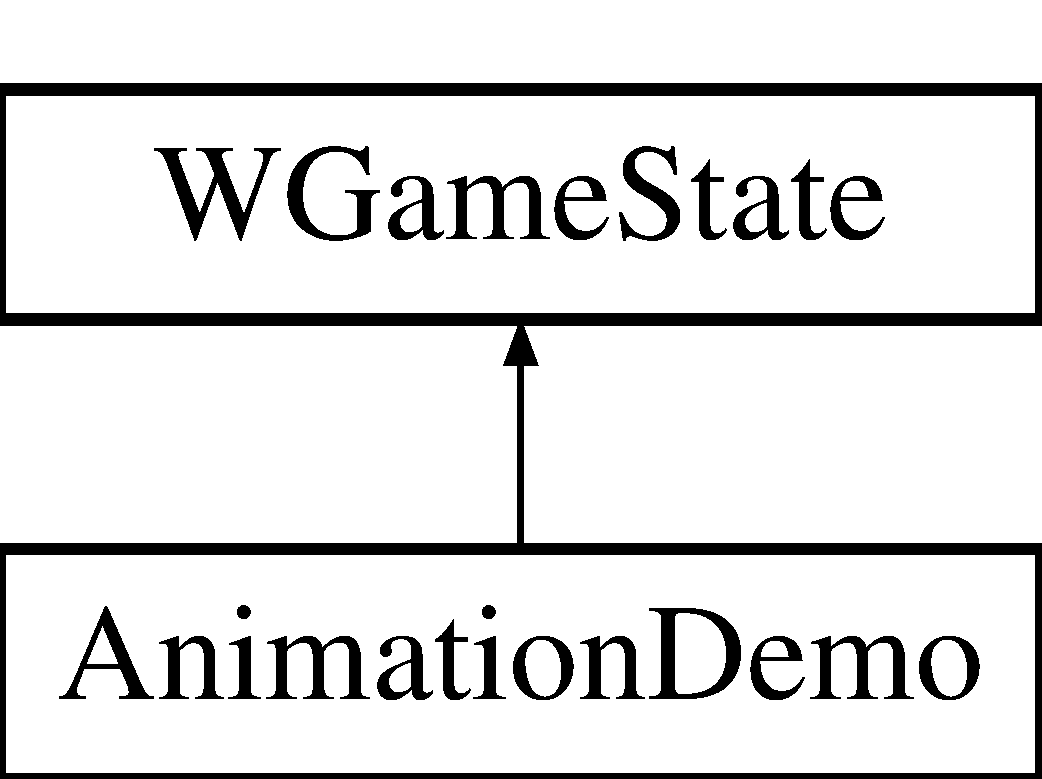
\includegraphics[height=2.000000cm]{class_animation_demo}
\end{center}
\end{figure}
\subsection*{Public Member Functions}
\begin{DoxyCompactItemize}
\item 
{\bfseries Animation\+Demo} (\hyperlink{class_wasabi}{Wasabi} $\ast$const app)\hypertarget{class_animation_demo_a5d8227106171fea6bbfde05f04f297cf}{}\label{class_animation_demo_a5d8227106171fea6bbfde05f04f297cf}

\item 
virtual void \hyperlink{class_animation_demo_aec31e9f0100b86674561ba14e16f364d}{Load} ()
\item 
virtual void \hyperlink{class_animation_demo_aa694b73bfa77098e98a77399655203c2}{Update} (float f\+Delta\+Time)
\item 
virtual void \hyperlink{class_animation_demo_a07d34d2c7f61565ac911d30216a9fb25}{Cleanup} ()
\end{DoxyCompactItemize}
\subsection*{Additional Inherited Members}


\subsection{Member Function Documentation}
\index{Animation\+Demo@{Animation\+Demo}!Cleanup@{Cleanup}}
\index{Cleanup@{Cleanup}!Animation\+Demo@{Animation\+Demo}}
\subsubsection[{\texorpdfstring{Cleanup()}{Cleanup()}}]{\setlength{\rightskip}{0pt plus 5cm}virtual void Animation\+Demo\+::\+Cleanup (
\begin{DoxyParamCaption}
{}
\end{DoxyParamCaption}
)\hspace{0.3cm}{\ttfamily [inline]}, {\ttfamily [virtual]}}\hypertarget{class_animation_demo_a07d34d2c7f61565ac911d30216a9fb25}{}\label{class_animation_demo_a07d34d2c7f61565ac911d30216a9fb25}
This function is called before this state is switched from. This gives the state a chance to clean up its resources before its destroyed. 

Reimplemented from \hyperlink{class_w_game_state_a50eddb2f648dc478ed0e10fee73fd4e9}{W\+Game\+State}.

\index{Animation\+Demo@{Animation\+Demo}!Load@{Load}}
\index{Load@{Load}!Animation\+Demo@{Animation\+Demo}}
\subsubsection[{\texorpdfstring{Load()}{Load()}}]{\setlength{\rightskip}{0pt plus 5cm}virtual void Animation\+Demo\+::\+Load (
\begin{DoxyParamCaption}
{}
\end{DoxyParamCaption}
)\hspace{0.3cm}{\ttfamily [inline]}, {\ttfamily [virtual]}}\hypertarget{class_animation_demo_aec31e9f0100b86674561ba14e16f364d}{}\label{class_animation_demo_aec31e9f0100b86674561ba14e16f364d}
This function, will be called every time this state is switched to. This gives the state a chance to load its resources. 

Reimplemented from \hyperlink{class_w_game_state_a20031e5724a12eb99aa81c013d1d9d63}{W\+Game\+State}.

\index{Animation\+Demo@{Animation\+Demo}!Update@{Update}}
\index{Update@{Update}!Animation\+Demo@{Animation\+Demo}}
\subsubsection[{\texorpdfstring{Update(float f\+Delta\+Time)}{Update(float fDeltaTime)}}]{\setlength{\rightskip}{0pt plus 5cm}virtual void Animation\+Demo\+::\+Update (
\begin{DoxyParamCaption}
\item[{float}]{f\+Delta\+Time}
\end{DoxyParamCaption}
)\hspace{0.3cm}{\ttfamily [inline]}, {\ttfamily [virtual]}}\hypertarget{class_animation_demo_aa694b73bfa77098e98a77399655203c2}{}\label{class_animation_demo_aa694b73bfa77098e98a77399655203c2}
This function is called every frame (right after \hyperlink{class_wasabi_ae7f699787307843fc886c4a9a09ebab7}{Wasabi\+::\+Loop()}) while the state is active. 
\begin{DoxyParams}{Parameters}
{\em f\+Delta\+Time} & The step time for this frame (roughly 1 / F\+PS) \\
\hline
\end{DoxyParams}


Reimplemented from \hyperlink{class_w_game_state_a5fe5a485ca56800cfd79237be2568d36}{W\+Game\+State}.



The documentation for this class was generated from the following file\+:\begin{DoxyCompactItemize}
\item 
Wasabi Test/Tests.\+cpp\end{DoxyCompactItemize}

\hypertarget{class_deferred_renderer_p_s}{}\section{Deferred\+Renderer\+PS Class Reference}
\label{class_deferred_renderer_p_s}\index{Deferred\+Renderer\+PS@{Deferred\+Renderer\+PS}}
Inheritance diagram for Deferred\+Renderer\+PS\+:\begin{figure}[H]
\begin{center}
\leavevmode
\includegraphics[height=3.000000cm]{class_deferred_renderer_p_s}
\end{center}
\end{figure}
\subsection*{Public Member Functions}
\begin{DoxyCompactItemize}
\item 
{\bfseries Deferred\+Renderer\+PS} (class \hyperlink{class_wasabi}{Wasabi} $\ast$const app)\hypertarget{class_deferred_renderer_p_s_ac0ca5a1f3051a866067132a435e73968}{}\label{class_deferred_renderer_p_s_ac0ca5a1f3051a866067132a435e73968}

\item 
virtual void {\bfseries Load} ()\hypertarget{class_deferred_renderer_p_s_af8c4e8d25a9d77dbaff0dfb45d6dfb07}{}\label{class_deferred_renderer_p_s_af8c4e8d25a9d77dbaff0dfb45d6dfb07}

\end{DoxyCompactItemize}
\subsection*{Additional Inherited Members}


The documentation for this class was generated from the following file\+:\begin{DoxyCompactItemize}
\item 
Wasabi/\+Renderers/W\+Deferred\+Renderer.\+cpp\end{DoxyCompactItemize}

\hypertarget{class_deferred_renderer_v_s}{}\section{Deferred\+Renderer\+VS Class Reference}
\label{class_deferred_renderer_v_s}\index{Deferred\+Renderer\+VS@{Deferred\+Renderer\+VS}}
Inheritance diagram for Deferred\+Renderer\+VS\+:\begin{figure}[H]
\begin{center}
\leavevmode
\includegraphics[height=3.000000cm]{class_deferred_renderer_v_s}
\end{center}
\end{figure}
\subsection*{Public Member Functions}
\begin{DoxyCompactItemize}
\item 
{\bfseries Deferred\+Renderer\+VS} (class \hyperlink{class_wasabi}{Wasabi} $\ast$const app)\hypertarget{class_deferred_renderer_v_s_a976a0e5a596f742cb7a64f91eee3f833}{}\label{class_deferred_renderer_v_s_a976a0e5a596f742cb7a64f91eee3f833}

\item 
virtual void \hyperlink{class_deferred_renderer_v_s_a35e479b4de6f046fa3b45e147eab3acf}{Load} ()
\end{DoxyCompactItemize}
\subsection*{Additional Inherited Members}


\subsection{Member Function Documentation}
\index{Deferred\+Renderer\+VS@{Deferred\+Renderer\+VS}!Load@{Load}}
\index{Load@{Load}!Deferred\+Renderer\+VS@{Deferred\+Renderer\+VS}}
\subsubsection[{\texorpdfstring{Load()}{Load()}}]{\setlength{\rightskip}{0pt plus 5cm}virtual void Deferred\+Renderer\+V\+S\+::\+Load (
\begin{DoxyParamCaption}
{}
\end{DoxyParamCaption}
)\hspace{0.3cm}{\ttfamily [inline]}, {\ttfamily [virtual]}}\hypertarget{class_deferred_renderer_v_s_a35e479b4de6f046fa3b45e147eab3acf}{}\label{class_deferred_renderer_v_s_a35e479b4de6f046fa3b45e147eab3acf}
Loads the shader into this object. This function must be implemented by a child class. The implemented function must fill in m\+\_\+module and m\+\_\+desc protected members to fully define the shader. See \hyperlink{class_w_shader}{W\+Shader} for example usage. 

Implements \hyperlink{class_w_shader_a7ce478193bc1676b1a7fdd741bdb32aa}{W\+Shader}.



The documentation for this class was generated from the following file\+:\begin{DoxyCompactItemize}
\item 
Wasabi/\+Renderers/W\+Deferred\+Renderer.\+cpp\end{DoxyCompactItemize}

\hypertarget{class_forward_renderer_p_s}{}\section{Forward\+Renderer\+PS Class Reference}
\label{class_forward_renderer_p_s}\index{Forward\+Renderer\+PS@{Forward\+Renderer\+PS}}
Inheritance diagram for Forward\+Renderer\+PS\+:\begin{figure}[H]
\begin{center}
\leavevmode
\includegraphics[height=3.000000cm]{class_forward_renderer_p_s}
\end{center}
\end{figure}
\subsection*{Public Member Functions}
\begin{DoxyCompactItemize}
\item 
{\bfseries Forward\+Renderer\+PS} (class \hyperlink{class_wasabi}{Wasabi} $\ast$const app)\hypertarget{class_forward_renderer_p_s_a6a1ed068b3859b8a06fdd1e7013f62da}{}\label{class_forward_renderer_p_s_a6a1ed068b3859b8a06fdd1e7013f62da}

\item 
virtual void \hyperlink{class_forward_renderer_p_s_abb142acd77b661e238ddcee56911f020}{Load} ()
\end{DoxyCompactItemize}
\subsection*{Additional Inherited Members}


\subsection{Member Function Documentation}
\index{Forward\+Renderer\+PS@{Forward\+Renderer\+PS}!Load@{Load}}
\index{Load@{Load}!Forward\+Renderer\+PS@{Forward\+Renderer\+PS}}
\subsubsection[{\texorpdfstring{Load()}{Load()}}]{\setlength{\rightskip}{0pt plus 5cm}virtual void Forward\+Renderer\+P\+S\+::\+Load (
\begin{DoxyParamCaption}
{}
\end{DoxyParamCaption}
)\hspace{0.3cm}{\ttfamily [inline]}, {\ttfamily [virtual]}}\hypertarget{class_forward_renderer_p_s_abb142acd77b661e238ddcee56911f020}{}\label{class_forward_renderer_p_s_abb142acd77b661e238ddcee56911f020}
Loads the shader into this object. This function must be implemented by a child class. The implemented function must fill in m\+\_\+module and m\+\_\+desc protected members to fully define the shader. See \hyperlink{class_w_shader}{W\+Shader} for example usage. 

Implements \hyperlink{class_w_shader_a7ce478193bc1676b1a7fdd741bdb32aa}{W\+Shader}.



The documentation for this class was generated from the following file\+:\begin{DoxyCompactItemize}
\item 
Wasabi/\+Renderers/W\+Forward\+Renderer.\+cpp\end{DoxyCompactItemize}

\hypertarget{class_forward_renderer_v_s}{}\section{Forward\+Renderer\+VS Class Reference}
\label{class_forward_renderer_v_s}\index{Forward\+Renderer\+VS@{Forward\+Renderer\+VS}}
Inheritance diagram for Forward\+Renderer\+VS\+:\begin{figure}[H]
\begin{center}
\leavevmode
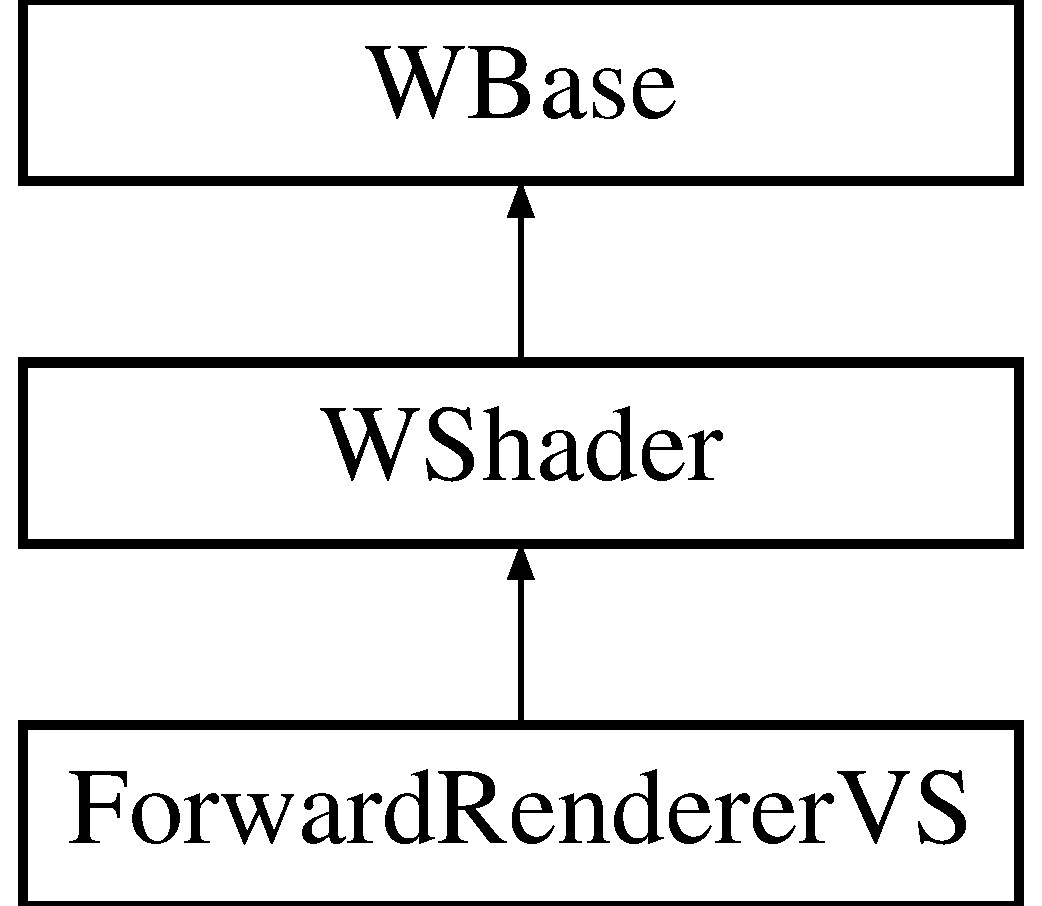
\includegraphics[height=3.000000cm]{class_forward_renderer_v_s}
\end{center}
\end{figure}
\subsection*{Public Member Functions}
\begin{DoxyCompactItemize}
\item 
{\bfseries Forward\+Renderer\+VS} (class \hyperlink{class_wasabi}{Wasabi} $\ast$const app)\hypertarget{class_forward_renderer_v_s_a25e4ba73eaef23c09749690ca1d1735f}{}\label{class_forward_renderer_v_s_a25e4ba73eaef23c09749690ca1d1735f}

\item 
virtual void {\bfseries Load} ()\hypertarget{class_forward_renderer_v_s_a68964f98fe8bec8f0addf39a4fcbe9fa}{}\label{class_forward_renderer_v_s_a68964f98fe8bec8f0addf39a4fcbe9fa}

\end{DoxyCompactItemize}
\subsection*{Additional Inherited Members}


The documentation for this class was generated from the following file\+:\begin{DoxyCompactItemize}
\item 
Wasabi/\+Renderers/W\+Forward\+Renderer.\+cpp\end{DoxyCompactItemize}

\hypertarget{class_instancing_demo}{}\section{Instancing\+Demo Class Reference}
\label{class_instancing_demo}\index{Instancing\+Demo@{Instancing\+Demo}}
Inheritance diagram for Instancing\+Demo\+:\begin{figure}[H]
\begin{center}
\leavevmode
\includegraphics[height=2.000000cm]{class_instancing_demo}
\end{center}
\end{figure}
\subsection*{Public Member Functions}
\begin{DoxyCompactItemize}
\item 
{\bfseries Instancing\+Demo} (\hyperlink{class_wasabi}{Wasabi} $\ast$const app)\hypertarget{class_instancing_demo_a090d90ceb1dd39ff1764f6dbb0ab3dbb}{}\label{class_instancing_demo_a090d90ceb1dd39ff1764f6dbb0ab3dbb}

\item 
virtual void \hyperlink{class_instancing_demo_abf05a0b6ce3814cb50cc43785f0f53c8}{Load} ()
\item 
virtual void \hyperlink{class_instancing_demo_a233c7a0d4552fc6a4c8f43a59b04f01c}{Update} (float f\+Delta\+Time)
\item 
virtual void \hyperlink{class_instancing_demo_a5c8e4cc00517e928128771f91028d473}{Cleanup} ()
\end{DoxyCompactItemize}
\subsection*{Additional Inherited Members}


\subsection{Member Function Documentation}
\index{Instancing\+Demo@{Instancing\+Demo}!Cleanup@{Cleanup}}
\index{Cleanup@{Cleanup}!Instancing\+Demo@{Instancing\+Demo}}
\subsubsection[{\texorpdfstring{Cleanup()}{Cleanup()}}]{\setlength{\rightskip}{0pt plus 5cm}virtual void Instancing\+Demo\+::\+Cleanup (
\begin{DoxyParamCaption}
{}
\end{DoxyParamCaption}
)\hspace{0.3cm}{\ttfamily [inline]}, {\ttfamily [virtual]}}\hypertarget{class_instancing_demo_a5c8e4cc00517e928128771f91028d473}{}\label{class_instancing_demo_a5c8e4cc00517e928128771f91028d473}
This function is called before this state is switched from. This gives the state a chance to clean up its resources before its destroyed. 

Reimplemented from \hyperlink{class_w_game_state_a50eddb2f648dc478ed0e10fee73fd4e9}{W\+Game\+State}.

\index{Instancing\+Demo@{Instancing\+Demo}!Load@{Load}}
\index{Load@{Load}!Instancing\+Demo@{Instancing\+Demo}}
\subsubsection[{\texorpdfstring{Load()}{Load()}}]{\setlength{\rightskip}{0pt plus 5cm}virtual void Instancing\+Demo\+::\+Load (
\begin{DoxyParamCaption}
{}
\end{DoxyParamCaption}
)\hspace{0.3cm}{\ttfamily [inline]}, {\ttfamily [virtual]}}\hypertarget{class_instancing_demo_abf05a0b6ce3814cb50cc43785f0f53c8}{}\label{class_instancing_demo_abf05a0b6ce3814cb50cc43785f0f53c8}
This function, will be called every time this state is switched to. This gives the state a chance to load its resources. 

Reimplemented from \hyperlink{class_w_game_state_a20031e5724a12eb99aa81c013d1d9d63}{W\+Game\+State}.

\index{Instancing\+Demo@{Instancing\+Demo}!Update@{Update}}
\index{Update@{Update}!Instancing\+Demo@{Instancing\+Demo}}
\subsubsection[{\texorpdfstring{Update(float f\+Delta\+Time)}{Update(float fDeltaTime)}}]{\setlength{\rightskip}{0pt plus 5cm}virtual void Instancing\+Demo\+::\+Update (
\begin{DoxyParamCaption}
\item[{float}]{f\+Delta\+Time}
\end{DoxyParamCaption}
)\hspace{0.3cm}{\ttfamily [inline]}, {\ttfamily [virtual]}}\hypertarget{class_instancing_demo_a233c7a0d4552fc6a4c8f43a59b04f01c}{}\label{class_instancing_demo_a233c7a0d4552fc6a4c8f43a59b04f01c}
This function is called every frame (right after \hyperlink{class_wasabi_ae7f699787307843fc886c4a9a09ebab7}{Wasabi\+::\+Loop()}) while the state is active. 
\begin{DoxyParams}{Parameters}
{\em f\+Delta\+Time} & The step time for this frame (roughly 1 / F\+PS) \\
\hline
\end{DoxyParams}


Reimplemented from \hyperlink{class_w_game_state_a5fe5a485ca56800cfd79237be2568d36}{W\+Game\+State}.



The documentation for this class was generated from the following file\+:\begin{DoxyCompactItemize}
\item 
Wasabi Test/Tests.\+cpp\end{DoxyCompactItemize}

\hypertarget{class_kofta}{}\section{Kofta Class Reference}
\label{class_kofta}\index{Kofta@{Kofta}}
Inheritance diagram for Kofta\+:\begin{figure}[H]
\begin{center}
\leavevmode
\includegraphics[height=2.000000cm]{class_kofta}
\end{center}
\end{figure}
\subsection*{Public Member Functions}
\begin{DoxyCompactItemize}
\item 
{\bfseries Kofta} (\hyperlink{class_wasabi}{Wasabi} $\ast$const app)\hypertarget{class_kofta_a8773a3ba38bee0c68a41aa326470aa7d}{}\label{class_kofta_a8773a3ba38bee0c68a41aa326470aa7d}

\item 
virtual void \hyperlink{class_kofta_a82e99828dc080cbc5a9cfc3db7b50081}{Load} ()
\item 
virtual void \hyperlink{class_kofta_a27da31ebb583a8a017061823ab6575da}{Update} (float f\+Delta\+Time)
\item 
void \hyperlink{class_kofta_a6650b02967c26d871e27aefd551e0c40}{Cleanup} ()
\end{DoxyCompactItemize}
\subsection*{Additional Inherited Members}


\subsection{Member Function Documentation}
\index{Kofta@{Kofta}!Cleanup@{Cleanup}}
\index{Cleanup@{Cleanup}!Kofta@{Kofta}}
\subsubsection[{\texorpdfstring{Cleanup()}{Cleanup()}}]{\setlength{\rightskip}{0pt plus 5cm}void Kofta\+::\+Cleanup (
\begin{DoxyParamCaption}
{}
\end{DoxyParamCaption}
)\hspace{0.3cm}{\ttfamily [inline]}, {\ttfamily [virtual]}}\hypertarget{class_kofta_a6650b02967c26d871e27aefd551e0c40}{}\label{class_kofta_a6650b02967c26d871e27aefd551e0c40}
This function is called before this state is switched from. This gives the state a chance to clean up its resources before its destroyed. 

Reimplemented from \hyperlink{class_w_game_state_a50eddb2f648dc478ed0e10fee73fd4e9}{W\+Game\+State}.

\index{Kofta@{Kofta}!Load@{Load}}
\index{Load@{Load}!Kofta@{Kofta}}
\subsubsection[{\texorpdfstring{Load()}{Load()}}]{\setlength{\rightskip}{0pt plus 5cm}virtual void Kofta\+::\+Load (
\begin{DoxyParamCaption}
{}
\end{DoxyParamCaption}
)\hspace{0.3cm}{\ttfamily [inline]}, {\ttfamily [virtual]}}\hypertarget{class_kofta_a82e99828dc080cbc5a9cfc3db7b50081}{}\label{class_kofta_a82e99828dc080cbc5a9cfc3db7b50081}
This function, will be called every time this state is switched to. This gives the state a chance to load its resources. 

Reimplemented from \hyperlink{class_w_game_state_a20031e5724a12eb99aa81c013d1d9d63}{W\+Game\+State}.

\index{Kofta@{Kofta}!Update@{Update}}
\index{Update@{Update}!Kofta@{Kofta}}
\subsubsection[{\texorpdfstring{Update(float f\+Delta\+Time)}{Update(float fDeltaTime)}}]{\setlength{\rightskip}{0pt plus 5cm}virtual void Kofta\+::\+Update (
\begin{DoxyParamCaption}
\item[{float}]{f\+Delta\+Time}
\end{DoxyParamCaption}
)\hspace{0.3cm}{\ttfamily [inline]}, {\ttfamily [virtual]}}\hypertarget{class_kofta_a27da31ebb583a8a017061823ab6575da}{}\label{class_kofta_a27da31ebb583a8a017061823ab6575da}
This function is called every frame (right after \hyperlink{class_wasabi_ae7f699787307843fc886c4a9a09ebab7}{Wasabi\+::\+Loop()}) while the state is active. 
\begin{DoxyParams}{Parameters}
{\em f\+Delta\+Time} & The step time for this frame (roughly 1 / F\+PS) \\
\hline
\end{DoxyParams}


Reimplemented from \hyperlink{class_w_game_state_a5fe5a485ca56800cfd79237be2568d36}{W\+Game\+State}.



The documentation for this class was generated from the following file\+:\begin{DoxyCompactItemize}
\item 
Wasabi Test/Tests.\+cpp\end{DoxyCompactItemize}

\hypertarget{struct_light_struct}{}\section{Light\+Struct Struct Reference}
\label{struct_light_struct}\index{Light\+Struct@{Light\+Struct}}
\subsection*{Public Attributes}
\begin{DoxyCompactItemize}
\item 
\hyperlink{class_w_vector4}{W\+Vector4} {\bfseries color}\hypertarget{struct_light_struct_a597e2bb30e3d7d2af0ce6d80468fc7c1}{}\label{struct_light_struct_a597e2bb30e3d7d2af0ce6d80468fc7c1}

\item 
\hyperlink{class_w_vector4}{W\+Vector4} {\bfseries dir}\hypertarget{struct_light_struct_a4ff553bc036087d0e2618516de2b039c}{}\label{struct_light_struct_a4ff553bc036087d0e2618516de2b039c}

\item 
\hyperlink{class_w_vector4}{W\+Vector4} {\bfseries pos}\hypertarget{struct_light_struct_a225084cf7f9e12887745f2bb1c8329e6}{}\label{struct_light_struct_a225084cf7f9e12887745f2bb1c8329e6}

\item 
int {\bfseries type}\hypertarget{struct_light_struct_a5b0efdd68d6ef9ef092f5d738e85ea9a}{}\label{struct_light_struct_a5b0efdd68d6ef9ef092f5d738e85ea9a}

\item 
float {\bfseries pad} \mbox{[}3\mbox{]}\hypertarget{struct_light_struct_ac2b200d24b5652dd0079e252b264177c}{}\label{struct_light_struct_ac2b200d24b5652dd0079e252b264177c}

\end{DoxyCompactItemize}


The documentation for this struct was generated from the following file\+:\begin{DoxyCompactItemize}
\item 
Wasabi/\+Renderers/W\+Forward\+Renderer.\+cpp\end{DoxyCompactItemize}

\hypertarget{class_sprite_geometry}{}\section{Sprite\+Geometry Class Reference}
\label{class_sprite_geometry}\index{Sprite\+Geometry@{Sprite\+Geometry}}
Inheritance diagram for Sprite\+Geometry\+:\begin{figure}[H]
\begin{center}
\leavevmode
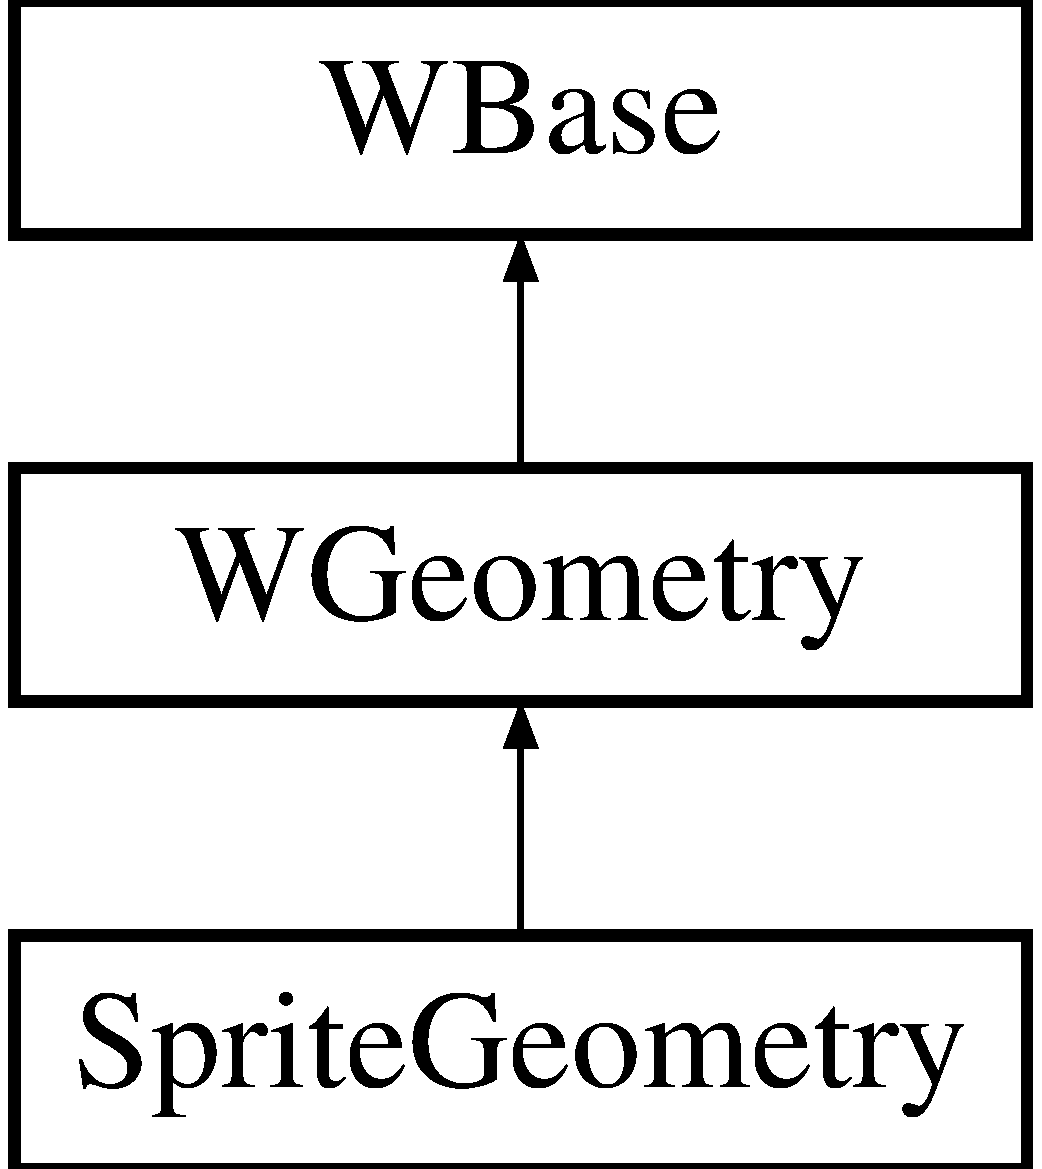
\includegraphics[height=3.000000cm]{class_sprite_geometry}
\end{center}
\end{figure}
\subsection*{Public Member Functions}
\begin{DoxyCompactItemize}
\item 
{\bfseries Sprite\+Geometry} (\hyperlink{class_wasabi}{Wasabi} $\ast$const app)\hypertarget{class_sprite_geometry_a597eab0671bcd1e06f2a30d13298d303}{}\label{class_sprite_geometry_a597eab0671bcd1e06f2a30d13298d303}

\item 
virtual unsigned int \hyperlink{class_sprite_geometry_a3c2a4c34292f6643f4bc7f375fe7ae68}{Get\+Vertex\+Buffer\+Count} () const 
\item 
virtual \hyperlink{struct_w___v_e_r_t_e_x___d_e_s_c_r_i_p_t_i_o_n}{W\+\_\+\+V\+E\+R\+T\+E\+X\+\_\+\+D\+E\+S\+C\+R\+I\+P\+T\+I\+ON} \hyperlink{class_sprite_geometry_a84172139912969ed1d36f48506f5918a}{Get\+Vertex\+Description} (unsigned int index) const 
\end{DoxyCompactItemize}
\subsection*{Additional Inherited Members}


\subsection{Member Function Documentation}
\index{Sprite\+Geometry@{Sprite\+Geometry}!Get\+Vertex\+Buffer\+Count@{Get\+Vertex\+Buffer\+Count}}
\index{Get\+Vertex\+Buffer\+Count@{Get\+Vertex\+Buffer\+Count}!Sprite\+Geometry@{Sprite\+Geometry}}
\subsubsection[{\texorpdfstring{Get\+Vertex\+Buffer\+Count() const }{GetVertexBufferCount() const }}]{\setlength{\rightskip}{0pt plus 5cm}virtual unsigned int Sprite\+Geometry\+::\+Get\+Vertex\+Buffer\+Count (
\begin{DoxyParamCaption}
{}
\end{DoxyParamCaption}
) const\hspace{0.3cm}{\ttfamily [inline]}, {\ttfamily [virtual]}}\hypertarget{class_sprite_geometry_a3c2a4c34292f6643f4bc7f375fe7ae68}{}\label{class_sprite_geometry_a3c2a4c34292f6643f4bc7f375fe7ae68}
This function should return the number of vertex descriptions that \hyperlink{class_sprite_geometry_a84172139912969ed1d36f48506f5918a}{Get\+Vertex\+Description()} can return, which represents the number of vertex buffers this geometry class can hold. \begin{DoxyReturn}{Returns}
The number of vertex buffers this geometry can hold 
\end{DoxyReturn}


Reimplemented from \hyperlink{class_w_geometry_a4eab34844955ef4583d393c3304d250c}{W\+Geometry}.

\index{Sprite\+Geometry@{Sprite\+Geometry}!Get\+Vertex\+Description@{Get\+Vertex\+Description}}
\index{Get\+Vertex\+Description@{Get\+Vertex\+Description}!Sprite\+Geometry@{Sprite\+Geometry}}
\subsubsection[{\texorpdfstring{Get\+Vertex\+Description(unsigned int index) const }{GetVertexDescription(unsigned int index) const }}]{\setlength{\rightskip}{0pt plus 5cm}virtual {\bf W\+\_\+\+V\+E\+R\+T\+E\+X\+\_\+\+D\+E\+S\+C\+R\+I\+P\+T\+I\+ON} Sprite\+Geometry\+::\+Get\+Vertex\+Description (
\begin{DoxyParamCaption}
\item[{unsigned int}]{layout\+\_\+index}
\end{DoxyParamCaption}
) const\hspace{0.3cm}{\ttfamily [inline]}, {\ttfamily [virtual]}}\hypertarget{class_sprite_geometry_a84172139912969ed1d36f48506f5918a}{}\label{class_sprite_geometry_a84172139912969ed1d36f48506f5918a}
Retrieves the vertex description of a vertex buffer. Should return valid descriptions for all {\itshape layout\+\_\+index} values between 0 and \hyperlink{class_sprite_geometry_a3c2a4c34292f6643f4bc7f375fe7ae68}{Get\+Vertex\+Buffer\+Count()}-\/1. 
\begin{DoxyParams}{Parameters}
{\em layout\+\_\+index} & Index of the vertex buffer \\
\hline
\end{DoxyParams}
\begin{DoxyReturn}{Returns}
The description of a vertex in the layout\+\_\+index \textquotesingle{}th vertex buffer 
\end{DoxyReturn}


Reimplemented from \hyperlink{class_w_geometry_a84409cef0ba8228b571f4f69cdfd6131}{W\+Geometry}.



The documentation for this class was generated from the following file\+:\begin{DoxyCompactItemize}
\item 
Wasabi/\+Sprites/W\+Sprite.\+cpp\end{DoxyCompactItemize}

\hypertarget{class_sprite_p_s}{}\section{Sprite\+PS Class Reference}
\label{class_sprite_p_s}\index{Sprite\+PS@{Sprite\+PS}}
Inheritance diagram for Sprite\+PS\+:\begin{figure}[H]
\begin{center}
\leavevmode
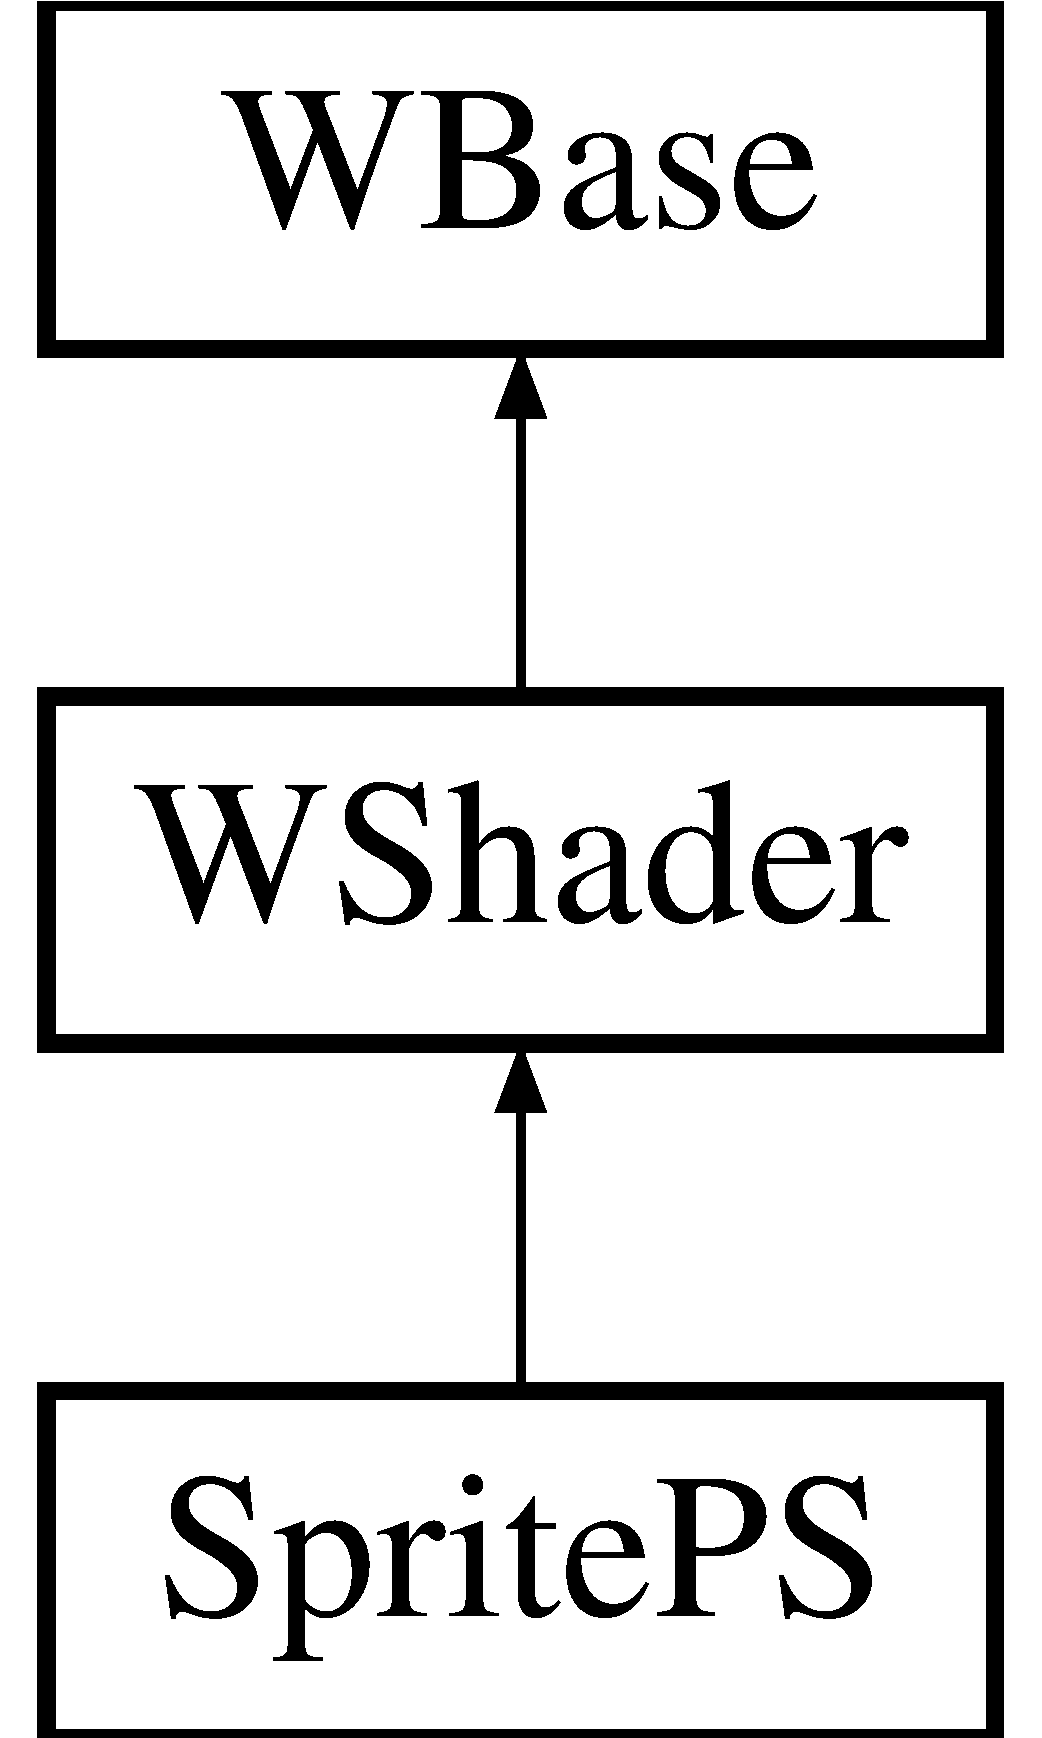
\includegraphics[height=3.000000cm]{class_sprite_p_s}
\end{center}
\end{figure}
\subsection*{Public Member Functions}
\begin{DoxyCompactItemize}
\item 
{\bfseries Sprite\+PS} (class \hyperlink{class_wasabi}{Wasabi} $\ast$const app)\hypertarget{class_sprite_p_s_a7b9bc0c25054aa821d27c0af7a6bd1e5}{}\label{class_sprite_p_s_a7b9bc0c25054aa821d27c0af7a6bd1e5}

\item 
virtual void {\bfseries Load} ()\hypertarget{class_sprite_p_s_a4791a5cc708e8419f6d8b20a64b678d3}{}\label{class_sprite_p_s_a4791a5cc708e8419f6d8b20a64b678d3}

\end{DoxyCompactItemize}
\subsection*{Additional Inherited Members}


The documentation for this class was generated from the following file\+:\begin{DoxyCompactItemize}
\item 
Wasabi/\+Sprites/W\+Sprite.\+cpp\end{DoxyCompactItemize}

\hypertarget{struct_sprite_vertex}{}\section{Sprite\+Vertex Struct Reference}
\label{struct_sprite_vertex}\index{Sprite\+Vertex@{Sprite\+Vertex}}
\subsection*{Public Attributes}
\begin{DoxyCompactItemize}
\item 
\hyperlink{class_w_vector2}{W\+Vector2} {\bfseries pos}\hypertarget{struct_sprite_vertex_ad0d8802b2bc8991337978071dfcb0066}{}\label{struct_sprite_vertex_ad0d8802b2bc8991337978071dfcb0066}

\item 
\hyperlink{class_w_vector2}{W\+Vector2} {\bfseries uv}\hypertarget{struct_sprite_vertex_a0cdd6a9b0cef246de78dad1f31f32885}{}\label{struct_sprite_vertex_a0cdd6a9b0cef246de78dad1f31f32885}

\end{DoxyCompactItemize}


The documentation for this struct was generated from the following file\+:\begin{DoxyCompactItemize}
\item 
Wasabi/\+Sprites/W\+Sprite.\+cpp\end{DoxyCompactItemize}

\hypertarget{class_sprite_v_s}{}\section{Sprite\+VS Class Reference}
\label{class_sprite_v_s}\index{Sprite\+VS@{Sprite\+VS}}
Inheritance diagram for Sprite\+VS\+:\begin{figure}[H]
\begin{center}
\leavevmode
\includegraphics[height=3.000000cm]{class_sprite_v_s}
\end{center}
\end{figure}
\subsection*{Public Member Functions}
\begin{DoxyCompactItemize}
\item 
{\bfseries Sprite\+VS} (class \hyperlink{class_wasabi}{Wasabi} $\ast$const app)\hypertarget{class_sprite_v_s_a3511fa72cef1eccc82028d14135a08cf}{}\label{class_sprite_v_s_a3511fa72cef1eccc82028d14135a08cf}

\item 
virtual void {\bfseries Load} ()\hypertarget{class_sprite_v_s_abd9362ef4fca5c252de18fcb089f7c40}{}\label{class_sprite_v_s_abd9362ef4fca5c252de18fcb089f7c40}

\end{DoxyCompactItemize}
\subsection*{Additional Inherited Members}


The documentation for this class was generated from the following file\+:\begin{DoxyCompactItemize}
\item 
Wasabi/\+Sprites/W\+Sprite.\+cpp\end{DoxyCompactItemize}

\hypertarget{class_text_geometry}{}\section{Text\+Geometry Class Reference}
\label{class_text_geometry}\index{Text\+Geometry@{Text\+Geometry}}
Inheritance diagram for Text\+Geometry\+:\begin{figure}[H]
\begin{center}
\leavevmode
\includegraphics[height=3.000000cm]{class_text_geometry}
\end{center}
\end{figure}
\subsection*{Public Member Functions}
\begin{DoxyCompactItemize}
\item 
{\bfseries Text\+Geometry} (\hyperlink{class_wasabi}{Wasabi} $\ast$const app)\hypertarget{class_text_geometry_a0986f8490b6a03fe4b63cef1d32b0ae8}{}\label{class_text_geometry_a0986f8490b6a03fe4b63cef1d32b0ae8}

\item 
virtual unsigned int \hyperlink{class_text_geometry_a0d6f019bc0034edcfdb51fe743e3b681}{Get\+Vertex\+Buffer\+Count} () const 
\item 
virtual \hyperlink{struct_w___v_e_r_t_e_x___d_e_s_c_r_i_p_t_i_o_n}{W\+\_\+\+V\+E\+R\+T\+E\+X\+\_\+\+D\+E\+S\+C\+R\+I\+P\+T\+I\+ON} \hyperlink{class_text_geometry_a048ec440054230443d89317dd09d2731}{Get\+Vertex\+Description} (unsigned int index) const 
\end{DoxyCompactItemize}
\subsection*{Additional Inherited Members}


\subsection{Member Function Documentation}
\index{Text\+Geometry@{Text\+Geometry}!Get\+Vertex\+Buffer\+Count@{Get\+Vertex\+Buffer\+Count}}
\index{Get\+Vertex\+Buffer\+Count@{Get\+Vertex\+Buffer\+Count}!Text\+Geometry@{Text\+Geometry}}
\subsubsection[{\texorpdfstring{Get\+Vertex\+Buffer\+Count() const }{GetVertexBufferCount() const }}]{\setlength{\rightskip}{0pt plus 5cm}virtual unsigned int Text\+Geometry\+::\+Get\+Vertex\+Buffer\+Count (
\begin{DoxyParamCaption}
{}
\end{DoxyParamCaption}
) const\hspace{0.3cm}{\ttfamily [inline]}, {\ttfamily [virtual]}}\hypertarget{class_text_geometry_a0d6f019bc0034edcfdb51fe743e3b681}{}\label{class_text_geometry_a0d6f019bc0034edcfdb51fe743e3b681}
This function should return the number of vertex descriptions that \hyperlink{class_text_geometry_a048ec440054230443d89317dd09d2731}{Get\+Vertex\+Description()} can return, which represents the number of vertex buffers this geometry class can hold. \begin{DoxyReturn}{Returns}
The number of vertex buffers this geometry can hold 
\end{DoxyReturn}


Reimplemented from \hyperlink{class_w_geometry_a4eab34844955ef4583d393c3304d250c}{W\+Geometry}.

\index{Text\+Geometry@{Text\+Geometry}!Get\+Vertex\+Description@{Get\+Vertex\+Description}}
\index{Get\+Vertex\+Description@{Get\+Vertex\+Description}!Text\+Geometry@{Text\+Geometry}}
\subsubsection[{\texorpdfstring{Get\+Vertex\+Description(unsigned int index) const }{GetVertexDescription(unsigned int index) const }}]{\setlength{\rightskip}{0pt plus 5cm}virtual {\bf W\+\_\+\+V\+E\+R\+T\+E\+X\+\_\+\+D\+E\+S\+C\+R\+I\+P\+T\+I\+ON} Text\+Geometry\+::\+Get\+Vertex\+Description (
\begin{DoxyParamCaption}
\item[{unsigned int}]{layout\+\_\+index}
\end{DoxyParamCaption}
) const\hspace{0.3cm}{\ttfamily [inline]}, {\ttfamily [virtual]}}\hypertarget{class_text_geometry_a048ec440054230443d89317dd09d2731}{}\label{class_text_geometry_a048ec440054230443d89317dd09d2731}
Retrieves the vertex description of a vertex buffer. Should return valid descriptions for all {\itshape layout\+\_\+index} values between 0 and \hyperlink{class_text_geometry_a0d6f019bc0034edcfdb51fe743e3b681}{Get\+Vertex\+Buffer\+Count()}-\/1. 
\begin{DoxyParams}{Parameters}
{\em layout\+\_\+index} & Index of the vertex buffer \\
\hline
\end{DoxyParams}
\begin{DoxyReturn}{Returns}
The description of a vertex in the layout\+\_\+index \textquotesingle{}th vertex buffer 
\end{DoxyReturn}


Reimplemented from \hyperlink{class_w_geometry_a84409cef0ba8228b571f4f69cdfd6131}{W\+Geometry}.



The documentation for this class was generated from the following file\+:\begin{DoxyCompactItemize}
\item 
Wasabi/\+Texts/W\+Text.\+cpp\end{DoxyCompactItemize}

\hypertarget{class_text_p_s}{}\section{Text\+PS Class Reference}
\label{class_text_p_s}\index{Text\+PS@{Text\+PS}}
Inheritance diagram for Text\+PS\+:\begin{figure}[H]
\begin{center}
\leavevmode
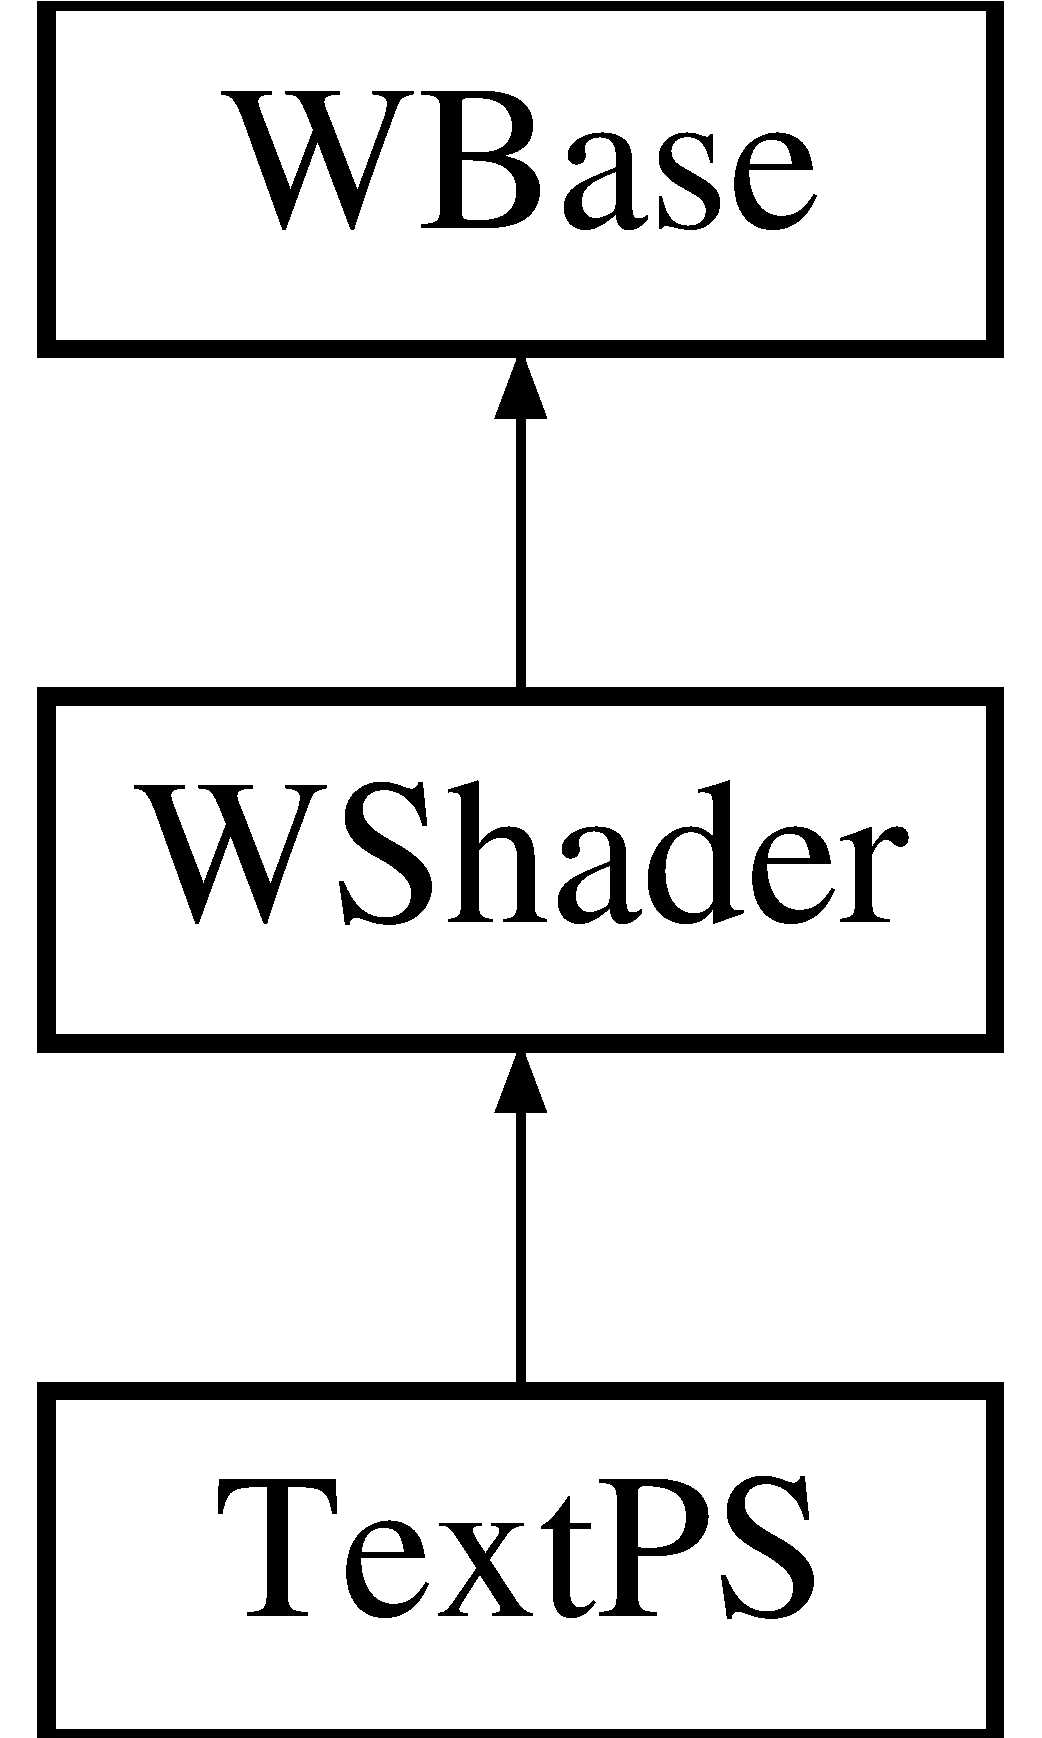
\includegraphics[height=3.000000cm]{class_text_p_s}
\end{center}
\end{figure}
\subsection*{Public Member Functions}
\begin{DoxyCompactItemize}
\item 
{\bfseries Text\+PS} (class \hyperlink{class_wasabi}{Wasabi} $\ast$const app)\hypertarget{class_text_p_s_a1d6339b4c0074363f17726ab72e84c91}{}\label{class_text_p_s_a1d6339b4c0074363f17726ab72e84c91}

\item 
virtual void {\bfseries Load} ()\hypertarget{class_text_p_s_af22b914fbd382746541d1cf04cf6a80f}{}\label{class_text_p_s_af22b914fbd382746541d1cf04cf6a80f}

\end{DoxyCompactItemize}
\subsection*{Additional Inherited Members}


The documentation for this class was generated from the following file\+:\begin{DoxyCompactItemize}
\item 
Wasabi/\+Texts/W\+Text.\+cpp\end{DoxyCompactItemize}

\hypertarget{struct_text_vertex}{}\section{Text\+Vertex Struct Reference}
\label{struct_text_vertex}\index{Text\+Vertex@{Text\+Vertex}}
\subsection*{Public Attributes}
\begin{DoxyCompactItemize}
\item 
\hyperlink{class_w_vector2}{W\+Vector2} {\bfseries pos}\hypertarget{struct_text_vertex_a38d1a81ac3af4575e07f94871e71b920}{}\label{struct_text_vertex_a38d1a81ac3af4575e07f94871e71b920}

\item 
\hyperlink{class_w_vector2}{W\+Vector2} {\bfseries uv}\hypertarget{struct_text_vertex_a501aec3b3873ebd1259af7075abc7b25}{}\label{struct_text_vertex_a501aec3b3873ebd1259af7075abc7b25}

\item 
\hyperlink{class_w_color}{W\+Color} {\bfseries col}\hypertarget{struct_text_vertex_a974333416415408a938fb478b5c44e40}{}\label{struct_text_vertex_a974333416415408a938fb478b5c44e40}

\end{DoxyCompactItemize}


The documentation for this struct was generated from the following file\+:\begin{DoxyCompactItemize}
\item 
Wasabi/\+Texts/W\+Text.\+cpp\end{DoxyCompactItemize}

\hypertarget{class_text_v_s}{}\section{Text\+VS Class Reference}
\label{class_text_v_s}\index{Text\+VS@{Text\+VS}}
Inheritance diagram for Text\+VS\+:\begin{figure}[H]
\begin{center}
\leavevmode
\includegraphics[height=3.000000cm]{class_text_v_s}
\end{center}
\end{figure}
\subsection*{Public Member Functions}
\begin{DoxyCompactItemize}
\item 
{\bfseries Text\+VS} (class \hyperlink{class_wasabi}{Wasabi} $\ast$const app)\hypertarget{class_text_v_s_a224ceb3b8ad79e2116702fa53ee18e7f}{}\label{class_text_v_s_a224ceb3b8ad79e2116702fa53ee18e7f}

\item 
virtual void \hyperlink{class_text_v_s_a5f5b2c085db4b90bc68f4c69434285ee}{Load} ()
\end{DoxyCompactItemize}
\subsection*{Additional Inherited Members}


\subsection{Member Function Documentation}
\index{Text\+VS@{Text\+VS}!Load@{Load}}
\index{Load@{Load}!Text\+VS@{Text\+VS}}
\subsubsection[{\texorpdfstring{Load()}{Load()}}]{\setlength{\rightskip}{0pt plus 5cm}virtual void Text\+V\+S\+::\+Load (
\begin{DoxyParamCaption}
{}
\end{DoxyParamCaption}
)\hspace{0.3cm}{\ttfamily [inline]}, {\ttfamily [virtual]}}\hypertarget{class_text_v_s_a5f5b2c085db4b90bc68f4c69434285ee}{}\label{class_text_v_s_a5f5b2c085db4b90bc68f4c69434285ee}
Loads the shader into this object. This function must be implemented by a child class. The implemented function must fill in m\+\_\+module and m\+\_\+desc protected members to fully define the shader. See \hyperlink{class_w_shader}{W\+Shader} for example usage. 

Implements \hyperlink{class_w_shader_a7ce478193bc1676b1a7fdd741bdb32aa}{W\+Shader}.



The documentation for this class was generated from the following file\+:\begin{DoxyCompactItemize}
\item 
Wasabi/\+Texts/W\+Text.\+cpp\end{DoxyCompactItemize}

\hypertarget{struct_w___b_o_u_n_d___r_e_s_o_u_r_c_e}{}\section{W\+\_\+\+B\+O\+U\+N\+D\+\_\+\+R\+E\+S\+O\+U\+R\+CE Struct Reference}
\label{struct_w___b_o_u_n_d___r_e_s_o_u_r_c_e}\index{W\+\_\+\+B\+O\+U\+N\+D\+\_\+\+R\+E\+S\+O\+U\+R\+CE@{W\+\_\+\+B\+O\+U\+N\+D\+\_\+\+R\+E\+S\+O\+U\+R\+CE}}
\subsection*{Public Member Functions}
\begin{DoxyCompactItemize}
\item 
{\bfseries W\+\_\+\+B\+O\+U\+N\+D\+\_\+\+R\+E\+S\+O\+U\+R\+CE} (W\+\_\+\+S\+H\+A\+D\+E\+R\+\_\+\+B\+O\+U\+N\+D\+\_\+\+R\+E\+S\+O\+U\+R\+C\+E\+\_\+\+T\+Y\+PE t, unsigned int index, std\+::vector$<$ \hyperlink{struct_w___s_h_a_d_e_r___v_a_r_i_a_b_l_e___i_n_f_o}{W\+\_\+\+S\+H\+A\+D\+E\+R\+\_\+\+V\+A\+R\+I\+A\+B\+L\+E\+\_\+\+I\+N\+FO} $>$ v=std\+::vector$<$ \hyperlink{struct_w___s_h_a_d_e_r___v_a_r_i_a_b_l_e___i_n_f_o}{W\+\_\+\+S\+H\+A\+D\+E\+R\+\_\+\+V\+A\+R\+I\+A\+B\+L\+E\+\_\+\+I\+N\+FO} $>$())\hypertarget{struct_w___b_o_u_n_d___r_e_s_o_u_r_c_e_a4e37d8d03ddab7339eb6b2b9e52453bd}{}\label{struct_w___b_o_u_n_d___r_e_s_o_u_r_c_e_a4e37d8d03ddab7339eb6b2b9e52453bd}

\item 
size\+\_\+t {\bfseries Get\+Size} ()\hypertarget{struct_w___b_o_u_n_d___r_e_s_o_u_r_c_e_a4316bb3b61abf67c9c4d1816175d38d1}{}\label{struct_w___b_o_u_n_d___r_e_s_o_u_r_c_e_a4316bb3b61abf67c9c4d1816175d38d1}

\end{DoxyCompactItemize}
\subsection*{Public Attributes}
\begin{DoxyCompactItemize}
\item 
W\+\_\+\+S\+H\+A\+D\+E\+R\+\_\+\+B\+O\+U\+N\+D\+\_\+\+R\+E\+S\+O\+U\+R\+C\+E\+\_\+\+T\+Y\+PE {\bfseries type}\hypertarget{struct_w___b_o_u_n_d___r_e_s_o_u_r_c_e_aba210bfb28ce06d4ab333eeab7877222}{}\label{struct_w___b_o_u_n_d___r_e_s_o_u_r_c_e_aba210bfb28ce06d4ab333eeab7877222}

\item 
unsigned int {\bfseries binding\+\_\+index}\hypertarget{struct_w___b_o_u_n_d___r_e_s_o_u_r_c_e_ae50619693d5d7b0ce92770fedebcf7a7}{}\label{struct_w___b_o_u_n_d___r_e_s_o_u_r_c_e_ae50619693d5d7b0ce92770fedebcf7a7}

\item 
std\+::vector$<$ \hyperlink{struct_w___s_h_a_d_e_r___v_a_r_i_a_b_l_e___i_n_f_o}{W\+\_\+\+S\+H\+A\+D\+E\+R\+\_\+\+V\+A\+R\+I\+A\+B\+L\+E\+\_\+\+I\+N\+FO} $>$ {\bfseries variables}\hypertarget{struct_w___b_o_u_n_d___r_e_s_o_u_r_c_e_a700e968f2052b08e3b2747c168f91f47}{}\label{struct_w___b_o_u_n_d___r_e_s_o_u_r_c_e_a700e968f2052b08e3b2747c168f91f47}

\end{DoxyCompactItemize}


The documentation for this struct was generated from the following files\+:\begin{DoxyCompactItemize}
\item 
Wasabi/\+Materials/W\+Effect.\+h\item 
Wasabi/\+Materials/W\+Effect.\+cpp\end{DoxyCompactItemize}

\hypertarget{struct_w___b_u_f_f_e_r}{}\section{W\+\_\+\+B\+U\+F\+F\+ER Struct Reference}
\label{struct_w___b_u_f_f_e_r}\index{W\+\_\+\+B\+U\+F\+F\+ER@{W\+\_\+\+B\+U\+F\+F\+ER}}


{\ttfamily \#include $<$W\+Core.\+h$>$}

\subsection*{Public Member Functions}
\begin{DoxyCompactItemize}
\item 
void \hyperlink{struct_w___b_u_f_f_e_r_a63033cffcf5f6d2a89b6eec48e3f9c1e}{Destroy} (Vk\+Device device)
\end{DoxyCompactItemize}
\subsection*{Public Attributes}
\begin{DoxyCompactItemize}
\item 
Vk\+Buffer \hyperlink{struct_w___b_u_f_f_e_r_ab54560f99cea81c48d1c386ec1e29a10}{buf}
\item 
Vk\+Device\+Memory \hyperlink{struct_w___b_u_f_f_e_r_af34fc1a3e7fb5994021ffbe323f77b8f}{mem}
\end{DoxyCompactItemize}


\subsection{Detailed Description}
Wrapper for a Vulkan buffer an its backing memory. 

\subsection{Member Function Documentation}
\index{W\+\_\+\+B\+U\+F\+F\+ER@{W\+\_\+\+B\+U\+F\+F\+ER}!Destroy@{Destroy}}
\index{Destroy@{Destroy}!W\+\_\+\+B\+U\+F\+F\+ER@{W\+\_\+\+B\+U\+F\+F\+ER}}
\subsubsection[{\texorpdfstring{Destroy(\+Vk\+Device device)}{Destroy(VkDevice device)}}]{\setlength{\rightskip}{0pt plus 5cm}void W\+\_\+\+B\+U\+F\+F\+E\+R\+::\+Destroy (
\begin{DoxyParamCaption}
\item[{Vk\+Device}]{device}
\end{DoxyParamCaption}
)\hspace{0.3cm}{\ttfamily [inline]}}\hypertarget{struct_w___b_u_f_f_e_r_a63033cffcf5f6d2a89b6eec48e3f9c1e}{}\label{struct_w___b_u_f_f_e_r_a63033cffcf5f6d2a89b6eec48e3f9c1e}
Destroy the buffer and its backing memory 
\begin{DoxyParams}{Parameters}
{\em device} & The Vulkan device used to crate the buffer \\
\hline
\end{DoxyParams}


\subsection{Member Data Documentation}
\index{W\+\_\+\+B\+U\+F\+F\+ER@{W\+\_\+\+B\+U\+F\+F\+ER}!buf@{buf}}
\index{buf@{buf}!W\+\_\+\+B\+U\+F\+F\+ER@{W\+\_\+\+B\+U\+F\+F\+ER}}
\subsubsection[{\texorpdfstring{buf}{buf}}]{\setlength{\rightskip}{0pt plus 5cm}Vk\+Buffer W\+\_\+\+B\+U\+F\+F\+E\+R\+::buf}\hypertarget{struct_w___b_u_f_f_e_r_ab54560f99cea81c48d1c386ec1e29a10}{}\label{struct_w___b_u_f_f_e_r_ab54560f99cea81c48d1c386ec1e29a10}
Vulkan buffer \index{W\+\_\+\+B\+U\+F\+F\+ER@{W\+\_\+\+B\+U\+F\+F\+ER}!mem@{mem}}
\index{mem@{mem}!W\+\_\+\+B\+U\+F\+F\+ER@{W\+\_\+\+B\+U\+F\+F\+ER}}
\subsubsection[{\texorpdfstring{mem}{mem}}]{\setlength{\rightskip}{0pt plus 5cm}Vk\+Device\+Memory W\+\_\+\+B\+U\+F\+F\+E\+R\+::mem}\hypertarget{struct_w___b_u_f_f_e_r_af34fc1a3e7fb5994021ffbe323f77b8f}{}\label{struct_w___b_u_f_f_e_r_af34fc1a3e7fb5994021ffbe323f77b8f}
buf\textquotesingle{}s backing memory 

The documentation for this struct was generated from the following file\+:\begin{DoxyCompactItemize}
\item 
Wasabi/\+Core/\hyperlink{_w_core_8h}{W\+Core.\+h}\end{DoxyCompactItemize}

\hypertarget{struct_w___f_o_n_t___o_b_j_e_c_t}{}\section{W\+\_\+\+F\+O\+N\+T\+\_\+\+O\+B\+J\+E\+CT Struct Reference}
\label{struct_w___f_o_n_t___o_b_j_e_c_t}\index{W\+\_\+\+F\+O\+N\+T\+\_\+\+O\+B\+J\+E\+CT@{W\+\_\+\+F\+O\+N\+T\+\_\+\+O\+B\+J\+E\+CT}}
\subsection*{Public Attributes}
\begin{DoxyCompactItemize}
\item 
unsigned int {\bfseries ID}\hypertarget{struct_w___f_o_n_t___o_b_j_e_c_t_ac0e5e46ec972c4d63b2b3fc450dafa30}{}\label{struct_w___f_o_n_t___o_b_j_e_c_t_ac0e5e46ec972c4d63b2b3fc450dafa30}

\item 
std\+::string {\bfseries name}\hypertarget{struct_w___f_o_n_t___o_b_j_e_c_t_a3800be882c77e0446b67d3b2eca7dc0b}{}\label{struct_w___f_o_n_t___o_b_j_e_c_t_a3800be882c77e0446b67d3b2eca7dc0b}

\item 
void $\ast$ {\bfseries cdata}\hypertarget{struct_w___f_o_n_t___o_b_j_e_c_t_a7cdc024c644c54076403becc319fb182}{}\label{struct_w___f_o_n_t___o_b_j_e_c_t_a7cdc024c644c54076403becc319fb182}

\item 
int {\bfseries num\+\_\+chars}\hypertarget{struct_w___f_o_n_t___o_b_j_e_c_t_ab98ffc9be0a2b149880f239593bc4efd}{}\label{struct_w___f_o_n_t___o_b_j_e_c_t_ab98ffc9be0a2b149880f239593bc4efd}

\item 
int {\bfseries char\+\_\+height}\hypertarget{struct_w___f_o_n_t___o_b_j_e_c_t_af976db051bf867e57ccf7a7f6824971c}{}\label{struct_w___f_o_n_t___o_b_j_e_c_t_af976db051bf867e57ccf7a7f6824971c}

\item 
class \hyperlink{class_w_geometry}{W\+Geometry} $\ast$ {\bfseries text\+Geometry}\hypertarget{struct_w___f_o_n_t___o_b_j_e_c_t_a3cb896037714c93e1af187c2a0a6d6a5}{}\label{struct_w___f_o_n_t___o_b_j_e_c_t_a3cb896037714c93e1af187c2a0a6d6a5}

\item 
class \hyperlink{class_w_material}{W\+Material} $\ast$ {\bfseries text\+Material}\hypertarget{struct_w___f_o_n_t___o_b_j_e_c_t_a3bc215907cb293a8df42260f21d74f76}{}\label{struct_w___f_o_n_t___o_b_j_e_c_t_a3bc215907cb293a8df42260f21d74f76}

\item 
class \hyperlink{class_w_image}{W\+Image} $\ast$ {\bfseries img}\hypertarget{struct_w___f_o_n_t___o_b_j_e_c_t_aeb5dce8b0ceac2046f3f75c589323ace}{}\label{struct_w___f_o_n_t___o_b_j_e_c_t_aeb5dce8b0ceac2046f3f75c589323ace}

\item 
vector$<$ \hyperlink{struct_w___r_e_n_d_e_r_i_n_g___t_e_x_t}{W\+\_\+\+R\+E\+N\+D\+E\+R\+I\+N\+G\+\_\+\+T\+E\+XT} $>$ {\bfseries texts}\hypertarget{struct_w___f_o_n_t___o_b_j_e_c_t_ad134e622cb6080cf466dd16676bbb5e0}{}\label{struct_w___f_o_n_t___o_b_j_e_c_t_ad134e622cb6080cf466dd16676bbb5e0}

\end{DoxyCompactItemize}


The documentation for this struct was generated from the following file\+:\begin{DoxyCompactItemize}
\item 
Wasabi/\+Texts/W\+Text.\+h\end{DoxyCompactItemize}

\hypertarget{struct_w___f_r_a_m_e}{}\section{W\+\_\+\+F\+R\+A\+ME Struct Reference}
\label{struct_w___f_r_a_m_e}\index{W\+\_\+\+F\+R\+A\+ME@{W\+\_\+\+F\+R\+A\+ME}}


{\ttfamily \#include $<$W\+Animation.\+h$>$}

Inheritance diagram for W\+\_\+\+F\+R\+A\+ME\+:\begin{figure}[H]
\begin{center}
\leavevmode
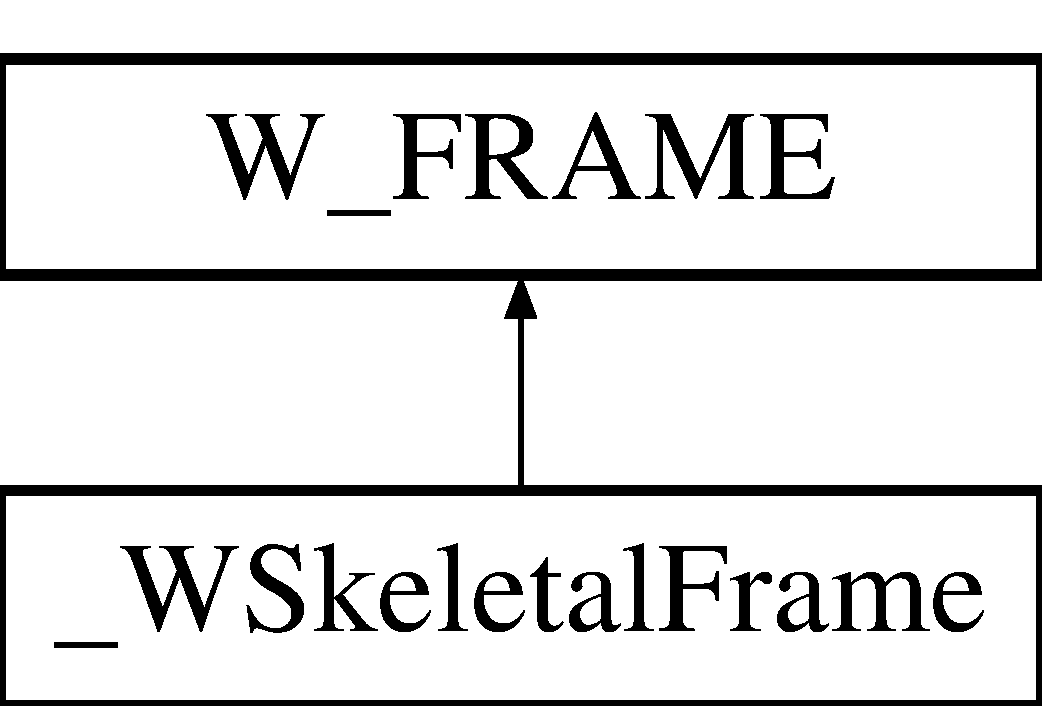
\includegraphics[height=2.000000cm]{struct_w___f_r_a_m_e}
\end{center}
\end{figure}
\subsection*{Public Attributes}
\begin{DoxyCompactItemize}
\item 
float \hyperlink{struct_w___f_r_a_m_e_a8b4bce41c5a65ffbc6058dec13213784}{f\+Time}
\end{DoxyCompactItemize}


\subsection{Detailed Description}
Represents an animation frame. 

\subsection{Member Data Documentation}
\index{W\+\_\+\+F\+R\+A\+ME@{W\+\_\+\+F\+R\+A\+ME}!f\+Time@{f\+Time}}
\index{f\+Time@{f\+Time}!W\+\_\+\+F\+R\+A\+ME@{W\+\_\+\+F\+R\+A\+ME}}
\subsubsection[{\texorpdfstring{f\+Time}{fTime}}]{\setlength{\rightskip}{0pt plus 5cm}float W\+\_\+\+F\+R\+A\+M\+E\+::f\+Time}\hypertarget{struct_w___f_r_a_m_e_a8b4bce41c5a65ffbc6058dec13213784}{}\label{struct_w___f_r_a_m_e_a8b4bce41c5a65ffbc6058dec13213784}
The duration of this frame. 

The documentation for this struct was generated from the following file\+:\begin{DoxyCompactItemize}
\item 
Wasabi/\+Animations/\hyperlink{_w_animation_8h}{W\+Animation.\+h}\end{DoxyCompactItemize}

\hypertarget{struct_w___i_n_p_u_t___l_a_y_o_u_t}{}\section{W\+\_\+\+I\+N\+P\+U\+T\+\_\+\+L\+A\+Y\+O\+UT Struct Reference}
\label{struct_w___i_n_p_u_t___l_a_y_o_u_t}\index{W\+\_\+\+I\+N\+P\+U\+T\+\_\+\+L\+A\+Y\+O\+UT@{W\+\_\+\+I\+N\+P\+U\+T\+\_\+\+L\+A\+Y\+O\+UT}}
\subsection*{Public Member Functions}
\begin{DoxyCompactItemize}
\item 
{\bfseries W\+\_\+\+I\+N\+P\+U\+T\+\_\+\+L\+A\+Y\+O\+UT} (std\+::vector$<$ \hyperlink{struct_w___s_h_a_d_e_r___v_a_r_i_a_b_l_e___i_n_f_o}{W\+\_\+\+S\+H\+A\+D\+E\+R\+\_\+\+V\+A\+R\+I\+A\+B\+L\+E\+\_\+\+I\+N\+FO} $>$ a, W\+\_\+\+V\+E\+R\+T\+E\+X\+\_\+\+I\+N\+P\+U\+T\+\_\+\+R\+A\+TE r=W\+\_\+\+I\+N\+P\+U\+T\+\_\+\+R\+A\+T\+E\+\_\+\+P\+E\+R\+\_\+\+V\+E\+R\+T\+EX)\hypertarget{struct_w___i_n_p_u_t___l_a_y_o_u_t_a7170e52b6b28b27eb67e0a2d790b6cf2}{}\label{struct_w___i_n_p_u_t___l_a_y_o_u_t_a7170e52b6b28b27eb67e0a2d790b6cf2}

\item 
size\+\_\+t {\bfseries Get\+Size} ()\hypertarget{struct_w___i_n_p_u_t___l_a_y_o_u_t_ad2f73e39a5198e328903616f627b313f}{}\label{struct_w___i_n_p_u_t___l_a_y_o_u_t_ad2f73e39a5198e328903616f627b313f}

\end{DoxyCompactItemize}
\subsection*{Public Attributes}
\begin{DoxyCompactItemize}
\item 
std\+::vector$<$ \hyperlink{struct_w___s_h_a_d_e_r___v_a_r_i_a_b_l_e___i_n_f_o}{W\+\_\+\+S\+H\+A\+D\+E\+R\+\_\+\+V\+A\+R\+I\+A\+B\+L\+E\+\_\+\+I\+N\+FO} $>$ {\bfseries attributes}\hypertarget{struct_w___i_n_p_u_t___l_a_y_o_u_t_aab71e215609c4b3a7c23e87fffdcb65e}{}\label{struct_w___i_n_p_u_t___l_a_y_o_u_t_aab71e215609c4b3a7c23e87fffdcb65e}

\item 
W\+\_\+\+V\+E\+R\+T\+E\+X\+\_\+\+I\+N\+P\+U\+T\+\_\+\+R\+A\+TE {\bfseries input\+\_\+rate}\hypertarget{struct_w___i_n_p_u_t___l_a_y_o_u_t_aa02f513ac0db3cbb549d4f5a48bb9fef}{}\label{struct_w___i_n_p_u_t___l_a_y_o_u_t_aa02f513ac0db3cbb549d4f5a48bb9fef}

\end{DoxyCompactItemize}


The documentation for this struct was generated from the following files\+:\begin{DoxyCompactItemize}
\item 
Wasabi/\+Materials/W\+Effect.\+h\item 
Wasabi/\+Materials/W\+Effect.\+cpp\end{DoxyCompactItemize}

\hypertarget{struct_w___r_a_y_c_a_s_t___o_u_t_p_u_t}{}\section{W\+\_\+\+R\+A\+Y\+C\+A\+S\+T\+\_\+\+O\+U\+T\+P\+UT Struct Reference}
\label{struct_w___r_a_y_c_a_s_t___o_u_t_p_u_t}\index{W\+\_\+\+R\+A\+Y\+C\+A\+S\+T\+\_\+\+O\+U\+T\+P\+UT@{W\+\_\+\+R\+A\+Y\+C\+A\+S\+T\+\_\+\+O\+U\+T\+P\+UT}}
\subsection*{Public Attributes}
\begin{DoxyCompactItemize}
\item 
float {\bfseries f\+Dist}\hypertarget{struct_w___r_a_y_c_a_s_t___o_u_t_p_u_t_a0162727e6735f350b4f2b3433880d30d}{}\label{struct_w___r_a_y_c_a_s_t___o_u_t_p_u_t_a0162727e6735f350b4f2b3433880d30d}

\item 
\hyperlink{class_w_vector3}{W\+Vector3} {\bfseries normal}\hypertarget{struct_w___r_a_y_c_a_s_t___o_u_t_p_u_t_a5e740ce2a9006f7f3dc2020c4f57f172}{}\label{struct_w___r_a_y_c_a_s_t___o_u_t_p_u_t_a5e740ce2a9006f7f3dc2020c4f57f172}

\end{DoxyCompactItemize}


The documentation for this struct was generated from the following file\+:\begin{DoxyCompactItemize}
\item 
Wasabi/\+Physics/W\+Physics\+Component.\+h\end{DoxyCompactItemize}

\hypertarget{struct_w___r_e_n_d_e_r_i_n_g___t_e_x_t}{}\section{W\+\_\+\+R\+E\+N\+D\+E\+R\+I\+N\+G\+\_\+\+T\+E\+XT Struct Reference}
\label{struct_w___r_e_n_d_e_r_i_n_g___t_e_x_t}\index{W\+\_\+\+R\+E\+N\+D\+E\+R\+I\+N\+G\+\_\+\+T\+E\+XT@{W\+\_\+\+R\+E\+N\+D\+E\+R\+I\+N\+G\+\_\+\+T\+E\+XT}}
\subsection*{Public Attributes}
\begin{DoxyCompactItemize}
\item 
std\+::string {\bfseries str}\hypertarget{struct_w___r_e_n_d_e_r_i_n_g___t_e_x_t_a6e33f0f43a0f769caf5bf09de1d67cff}{}\label{struct_w___r_e_n_d_e_r_i_n_g___t_e_x_t_a6e33f0f43a0f769caf5bf09de1d67cff}

\item 
\hyperlink{class_w_color}{W\+Color} {\bfseries col}\hypertarget{struct_w___r_e_n_d_e_r_i_n_g___t_e_x_t_a94e310a92f39f1d4e0daa86b8affdb7d}{}\label{struct_w___r_e_n_d_e_r_i_n_g___t_e_x_t_a94e310a92f39f1d4e0daa86b8affdb7d}

\item 
float {\bfseries f\+Height}\hypertarget{struct_w___r_e_n_d_e_r_i_n_g___t_e_x_t_a0560a22b80dd517ec081d90ee03a43e1}{}\label{struct_w___r_e_n_d_e_r_i_n_g___t_e_x_t_a0560a22b80dd517ec081d90ee03a43e1}

\item 
int {\bfseries x}\hypertarget{struct_w___r_e_n_d_e_r_i_n_g___t_e_x_t_ab538b386bcacb874986397e2109f1c86}{}\label{struct_w___r_e_n_d_e_r_i_n_g___t_e_x_t_ab538b386bcacb874986397e2109f1c86}

\item 
int {\bfseries y}\hypertarget{struct_w___r_e_n_d_e_r_i_n_g___t_e_x_t_af24246ee5733da8d0d4a4b8653fed020}{}\label{struct_w___r_e_n_d_e_r_i_n_g___t_e_x_t_af24246ee5733da8d0d4a4b8653fed020}

\end{DoxyCompactItemize}


The documentation for this struct was generated from the following file\+:\begin{DoxyCompactItemize}
\item 
Wasabi/\+Texts/W\+Text.\+h\end{DoxyCompactItemize}

\hypertarget{struct_w___s_h_a_d_e_r___d_e_s_c}{}\section{W\+\_\+\+S\+H\+A\+D\+E\+R\+\_\+\+D\+E\+SC Struct Reference}
\label{struct_w___s_h_a_d_e_r___d_e_s_c}\index{W\+\_\+\+S\+H\+A\+D\+E\+R\+\_\+\+D\+E\+SC@{W\+\_\+\+S\+H\+A\+D\+E\+R\+\_\+\+D\+E\+SC}}


{\ttfamily \#include $<$W\+Effect.\+h$>$}

\subsection*{Public Attributes}
\begin{DoxyCompactItemize}
\item 
\hyperlink{group__engineclass_ga8a79e4a3a441c88450e176150102c7b7}{W\+\_\+\+S\+H\+A\+D\+E\+R\+\_\+\+T\+Y\+PE} \hyperlink{struct_w___s_h_a_d_e_r___d_e_s_c_ad7b83db0ce3b5eb747a0fea76b52acd5}{type}
\item 
std\+::vector$<$ \hyperlink{struct_w___b_o_u_n_d___r_e_s_o_u_r_c_e}{W\+\_\+\+B\+O\+U\+N\+D\+\_\+\+R\+E\+S\+O\+U\+R\+CE} $>$ \hyperlink{struct_w___s_h_a_d_e_r___d_e_s_c_aa3fea1cc775493c0fe9590129f91df63}{bound\+\_\+resources}
\item 
std\+::vector$<$ \hyperlink{struct_w___i_n_p_u_t___l_a_y_o_u_t}{W\+\_\+\+I\+N\+P\+U\+T\+\_\+\+L\+A\+Y\+O\+UT} $>$ \hyperlink{struct_w___s_h_a_d_e_r___d_e_s_c_a994385c2ccd44ff6b0879ac15ba035cd}{input\+\_\+layouts}
\item 
unsigned int \hyperlink{struct_w___s_h_a_d_e_r___d_e_s_c_ac1b40ff1facba393210a61aeb5a064ea}{animation\+\_\+texture\+\_\+index}
\item 
unsigned int \hyperlink{struct_w___s_h_a_d_e_r___d_e_s_c_a23a05bd7613ca8b029f14e27130a7844}{instancing\+\_\+texture\+\_\+index}
\end{DoxyCompactItemize}


\subsection{Detailed Description}
Description of a shader to be bound to an effect. 

\subsection{Member Data Documentation}
\index{W\+\_\+\+S\+H\+A\+D\+E\+R\+\_\+\+D\+E\+SC@{W\+\_\+\+S\+H\+A\+D\+E\+R\+\_\+\+D\+E\+SC}!animation\+\_\+texture\+\_\+index@{animation\+\_\+texture\+\_\+index}}
\index{animation\+\_\+texture\+\_\+index@{animation\+\_\+texture\+\_\+index}!W\+\_\+\+S\+H\+A\+D\+E\+R\+\_\+\+D\+E\+SC@{W\+\_\+\+S\+H\+A\+D\+E\+R\+\_\+\+D\+E\+SC}}
\subsubsection[{\texorpdfstring{animation\+\_\+texture\+\_\+index}{animation_texture_index}}]{\setlength{\rightskip}{0pt plus 5cm}unsigned int W\+\_\+\+S\+H\+A\+D\+E\+R\+\_\+\+D\+E\+S\+C\+::animation\+\_\+texture\+\_\+index}\hypertarget{struct_w___s_h_a_d_e_r___d_e_s_c_ac1b40ff1facba393210a61aeb5a064ea}{}\label{struct_w___s_h_a_d_e_r___d_e_s_c_ac1b40ff1facba393210a61aeb5a064ea}
Binding index of a texture (which must exist in bound\+\_\+resources) that has been specifically marked to be used for animation \index{W\+\_\+\+S\+H\+A\+D\+E\+R\+\_\+\+D\+E\+SC@{W\+\_\+\+S\+H\+A\+D\+E\+R\+\_\+\+D\+E\+SC}!bound\+\_\+resources@{bound\+\_\+resources}}
\index{bound\+\_\+resources@{bound\+\_\+resources}!W\+\_\+\+S\+H\+A\+D\+E\+R\+\_\+\+D\+E\+SC@{W\+\_\+\+S\+H\+A\+D\+E\+R\+\_\+\+D\+E\+SC}}
\subsubsection[{\texorpdfstring{bound\+\_\+resources}{bound_resources}}]{\setlength{\rightskip}{0pt plus 5cm}std\+::vector$<${\bf W\+\_\+\+B\+O\+U\+N\+D\+\_\+\+R\+E\+S\+O\+U\+R\+CE}$>$ W\+\_\+\+S\+H\+A\+D\+E\+R\+\_\+\+D\+E\+S\+C\+::bound\+\_\+resources}\hypertarget{struct_w___s_h_a_d_e_r___d_e_s_c_aa3fea1cc775493c0fe9590129f91df63}{}\label{struct_w___s_h_a_d_e_r___d_e_s_c_aa3fea1cc775493c0fe9590129f91df63}
A list of bound resources (including U\+B\+Os and samplers/textures) \index{W\+\_\+\+S\+H\+A\+D\+E\+R\+\_\+\+D\+E\+SC@{W\+\_\+\+S\+H\+A\+D\+E\+R\+\_\+\+D\+E\+SC}!input\+\_\+layouts@{input\+\_\+layouts}}
\index{input\+\_\+layouts@{input\+\_\+layouts}!W\+\_\+\+S\+H\+A\+D\+E\+R\+\_\+\+D\+E\+SC@{W\+\_\+\+S\+H\+A\+D\+E\+R\+\_\+\+D\+E\+SC}}
\subsubsection[{\texorpdfstring{input\+\_\+layouts}{input_layouts}}]{\setlength{\rightskip}{0pt plus 5cm}std\+::vector$<${\bf W\+\_\+\+I\+N\+P\+U\+T\+\_\+\+L\+A\+Y\+O\+UT}$>$ W\+\_\+\+S\+H\+A\+D\+E\+R\+\_\+\+D\+E\+S\+C\+::input\+\_\+layouts}\hypertarget{struct_w___s_h_a_d_e_r___d_e_s_c_a994385c2ccd44ff6b0879ac15ba035cd}{}\label{struct_w___s_h_a_d_e_r___d_e_s_c_a994385c2ccd44ff6b0879ac15ba035cd}
A list of input layouts that bind to the shader. There should be one vertex buffer present to bind to every input layout in the shader \index{W\+\_\+\+S\+H\+A\+D\+E\+R\+\_\+\+D\+E\+SC@{W\+\_\+\+S\+H\+A\+D\+E\+R\+\_\+\+D\+E\+SC}!instancing\+\_\+texture\+\_\+index@{instancing\+\_\+texture\+\_\+index}}
\index{instancing\+\_\+texture\+\_\+index@{instancing\+\_\+texture\+\_\+index}!W\+\_\+\+S\+H\+A\+D\+E\+R\+\_\+\+D\+E\+SC@{W\+\_\+\+S\+H\+A\+D\+E\+R\+\_\+\+D\+E\+SC}}
\subsubsection[{\texorpdfstring{instancing\+\_\+texture\+\_\+index}{instancing_texture_index}}]{\setlength{\rightskip}{0pt plus 5cm}unsigned int W\+\_\+\+S\+H\+A\+D\+E\+R\+\_\+\+D\+E\+S\+C\+::instancing\+\_\+texture\+\_\+index}\hypertarget{struct_w___s_h_a_d_e_r___d_e_s_c_a23a05bd7613ca8b029f14e27130a7844}{}\label{struct_w___s_h_a_d_e_r___d_e_s_c_a23a05bd7613ca8b029f14e27130a7844}
Binding index of a texture (which must exist in bound\+\_\+resources) that has been specifically marked to be used for instancing \index{W\+\_\+\+S\+H\+A\+D\+E\+R\+\_\+\+D\+E\+SC@{W\+\_\+\+S\+H\+A\+D\+E\+R\+\_\+\+D\+E\+SC}!type@{type}}
\index{type@{type}!W\+\_\+\+S\+H\+A\+D\+E\+R\+\_\+\+D\+E\+SC@{W\+\_\+\+S\+H\+A\+D\+E\+R\+\_\+\+D\+E\+SC}}
\subsubsection[{\texorpdfstring{type}{type}}]{\setlength{\rightskip}{0pt plus 5cm}{\bf W\+\_\+\+S\+H\+A\+D\+E\+R\+\_\+\+T\+Y\+PE} W\+\_\+\+S\+H\+A\+D\+E\+R\+\_\+\+D\+E\+S\+C\+::type}\hypertarget{struct_w___s_h_a_d_e_r___d_e_s_c_ad7b83db0ce3b5eb747a0fea76b52acd5}{}\label{struct_w___s_h_a_d_e_r___d_e_s_c_ad7b83db0ce3b5eb747a0fea76b52acd5}
Type of the shader 

The documentation for this struct was generated from the following file\+:\begin{DoxyCompactItemize}
\item 
Wasabi/\+Materials/\hyperlink{_w_effect_8h}{W\+Effect.\+h}\end{DoxyCompactItemize}

\hypertarget{struct_w___s_h_a_d_e_r___v_a_r_i_a_b_l_e___i_n_f_o}{}\section{W\+\_\+\+S\+H\+A\+D\+E\+R\+\_\+\+V\+A\+R\+I\+A\+B\+L\+E\+\_\+\+I\+N\+FO Struct Reference}
\label{struct_w___s_h_a_d_e_r___v_a_r_i_a_b_l_e___i_n_f_o}\index{W\+\_\+\+S\+H\+A\+D\+E\+R\+\_\+\+V\+A\+R\+I\+A\+B\+L\+E\+\_\+\+I\+N\+FO@{W\+\_\+\+S\+H\+A\+D\+E\+R\+\_\+\+V\+A\+R\+I\+A\+B\+L\+E\+\_\+\+I\+N\+FO}}


{\ttfamily \#include $<$W\+Effect.\+h$>$}

\subsection*{Public Member Functions}
\begin{DoxyCompactItemize}
\item 
{\bfseries W\+\_\+\+S\+H\+A\+D\+E\+R\+\_\+\+V\+A\+R\+I\+A\+B\+L\+E\+\_\+\+I\+N\+FO} (\hyperlink{group__engineclass_gaeca2b79f62ba669ae9c5dbc516b66522}{W\+\_\+\+S\+H\+A\+D\+E\+R\+\_\+\+V\+A\+R\+I\+A\+B\+L\+E\+\_\+\+T\+Y\+PE} \+\_\+type, int \+\_\+num\+\_\+elems, std\+::string \+\_\+name=\char`\"{}\char`\"{})\hypertarget{struct_w___s_h_a_d_e_r___v_a_r_i_a_b_l_e___i_n_f_o_a7146ac62a2911ba861d9661debb7fac5}{}\label{struct_w___s_h_a_d_e_r___v_a_r_i_a_b_l_e___i_n_f_o_a7146ac62a2911ba861d9661debb7fac5}

\item 
size\+\_\+t \hyperlink{struct_w___s_h_a_d_e_r___v_a_r_i_a_b_l_e___i_n_f_o_aa18e0f7e7d80c98ddcbaeaa55649fc22}{Get\+Size} ()
\item 
Vk\+Format \hyperlink{struct_w___s_h_a_d_e_r___v_a_r_i_a_b_l_e___i_n_f_o_ab9e7bb852fada1b45ec4af82d30cb484}{Get\+Format} ()
\end{DoxyCompactItemize}
\subsection*{Public Attributes}
\begin{DoxyCompactItemize}
\item 
\hyperlink{group__engineclass_gaeca2b79f62ba669ae9c5dbc516b66522}{W\+\_\+\+S\+H\+A\+D\+E\+R\+\_\+\+V\+A\+R\+I\+A\+B\+L\+E\+\_\+\+T\+Y\+PE} \hyperlink{struct_w___s_h_a_d_e_r___v_a_r_i_a_b_l_e___i_n_f_o_a8dd6afc8a043c57343a7e401dffaaa0b}{type}
\item 
int \hyperlink{struct_w___s_h_a_d_e_r___v_a_r_i_a_b_l_e___i_n_f_o_a76488ce65cd829ddc892ebd86560b889}{num\+\_\+elems}
\item 
std\+::string \hyperlink{struct_w___s_h_a_d_e_r___v_a_r_i_a_b_l_e___i_n_f_o_a6c7ea051bec0e855ef7531ac619eacc4}{name}
\end{DoxyCompactItemize}


\subsection{Detailed Description}
Description of a shader variable in a U\+BO or vertex attribute. 

\subsection{Member Function Documentation}
\index{W\+\_\+\+S\+H\+A\+D\+E\+R\+\_\+\+V\+A\+R\+I\+A\+B\+L\+E\+\_\+\+I\+N\+FO@{W\+\_\+\+S\+H\+A\+D\+E\+R\+\_\+\+V\+A\+R\+I\+A\+B\+L\+E\+\_\+\+I\+N\+FO}!Get\+Format@{Get\+Format}}
\index{Get\+Format@{Get\+Format}!W\+\_\+\+S\+H\+A\+D\+E\+R\+\_\+\+V\+A\+R\+I\+A\+B\+L\+E\+\_\+\+I\+N\+FO@{W\+\_\+\+S\+H\+A\+D\+E\+R\+\_\+\+V\+A\+R\+I\+A\+B\+L\+E\+\_\+\+I\+N\+FO}}
\subsubsection[{\texorpdfstring{Get\+Format()}{GetFormat()}}]{\setlength{\rightskip}{0pt plus 5cm}Vk\+Format W\+\_\+\+S\+H\+A\+D\+E\+R\+\_\+\+V\+A\+R\+I\+A\+B\+L\+E\+\_\+\+I\+N\+F\+O\+::\+Get\+Format (
\begin{DoxyParamCaption}
{}
\end{DoxyParamCaption}
)}\hypertarget{struct_w___s_h_a_d_e_r___v_a_r_i_a_b_l_e___i_n_f_o_ab9e7bb852fada1b45ec4af82d30cb484}{}\label{struct_w___s_h_a_d_e_r___v_a_r_i_a_b_l_e___i_n_f_o_ab9e7bb852fada1b45ec4af82d30cb484}
Retrieves the Vulkan format corresponding to this variable. \begin{DoxyReturn}{Returns}
Format of the the variable 
\end{DoxyReturn}
\index{W\+\_\+\+S\+H\+A\+D\+E\+R\+\_\+\+V\+A\+R\+I\+A\+B\+L\+E\+\_\+\+I\+N\+FO@{W\+\_\+\+S\+H\+A\+D\+E\+R\+\_\+\+V\+A\+R\+I\+A\+B\+L\+E\+\_\+\+I\+N\+FO}!Get\+Size@{Get\+Size}}
\index{Get\+Size@{Get\+Size}!W\+\_\+\+S\+H\+A\+D\+E\+R\+\_\+\+V\+A\+R\+I\+A\+B\+L\+E\+\_\+\+I\+N\+FO@{W\+\_\+\+S\+H\+A\+D\+E\+R\+\_\+\+V\+A\+R\+I\+A\+B\+L\+E\+\_\+\+I\+N\+FO}}
\subsubsection[{\texorpdfstring{Get\+Size()}{GetSize()}}]{\setlength{\rightskip}{0pt plus 5cm}size\+\_\+t W\+\_\+\+S\+H\+A\+D\+E\+R\+\_\+\+V\+A\+R\+I\+A\+B\+L\+E\+\_\+\+I\+N\+F\+O\+::\+Get\+Size (
\begin{DoxyParamCaption}
{}
\end{DoxyParamCaption}
)}\hypertarget{struct_w___s_h_a_d_e_r___v_a_r_i_a_b_l_e___i_n_f_o_aa18e0f7e7d80c98ddcbaeaa55649fc22}{}\label{struct_w___s_h_a_d_e_r___v_a_r_i_a_b_l_e___i_n_f_o_aa18e0f7e7d80c98ddcbaeaa55649fc22}
Retrieves the size of the variable, in bytes. This is calculated as the size of type multiplied by num\+\_\+elems. \begin{DoxyReturn}{Returns}
Size, in bytes, of this shader variable 
\end{DoxyReturn}


\subsection{Member Data Documentation}
\index{W\+\_\+\+S\+H\+A\+D\+E\+R\+\_\+\+V\+A\+R\+I\+A\+B\+L\+E\+\_\+\+I\+N\+FO@{W\+\_\+\+S\+H\+A\+D\+E\+R\+\_\+\+V\+A\+R\+I\+A\+B\+L\+E\+\_\+\+I\+N\+FO}!name@{name}}
\index{name@{name}!W\+\_\+\+S\+H\+A\+D\+E\+R\+\_\+\+V\+A\+R\+I\+A\+B\+L\+E\+\_\+\+I\+N\+FO@{W\+\_\+\+S\+H\+A\+D\+E\+R\+\_\+\+V\+A\+R\+I\+A\+B\+L\+E\+\_\+\+I\+N\+FO}}
\subsubsection[{\texorpdfstring{name}{name}}]{\setlength{\rightskip}{0pt plus 5cm}std\+::string W\+\_\+\+S\+H\+A\+D\+E\+R\+\_\+\+V\+A\+R\+I\+A\+B\+L\+E\+\_\+\+I\+N\+F\+O\+::name}\hypertarget{struct_w___s_h_a_d_e_r___v_a_r_i_a_b_l_e___i_n_f_o_a6c7ea051bec0e855ef7531ac619eacc4}{}\label{struct_w___s_h_a_d_e_r___v_a_r_i_a_b_l_e___i_n_f_o_a6c7ea051bec0e855ef7531ac619eacc4}
Given name for the variable, which is used by materials to set its value \index{W\+\_\+\+S\+H\+A\+D\+E\+R\+\_\+\+V\+A\+R\+I\+A\+B\+L\+E\+\_\+\+I\+N\+FO@{W\+\_\+\+S\+H\+A\+D\+E\+R\+\_\+\+V\+A\+R\+I\+A\+B\+L\+E\+\_\+\+I\+N\+FO}!num\+\_\+elems@{num\+\_\+elems}}
\index{num\+\_\+elems@{num\+\_\+elems}!W\+\_\+\+S\+H\+A\+D\+E\+R\+\_\+\+V\+A\+R\+I\+A\+B\+L\+E\+\_\+\+I\+N\+FO@{W\+\_\+\+S\+H\+A\+D\+E\+R\+\_\+\+V\+A\+R\+I\+A\+B\+L\+E\+\_\+\+I\+N\+FO}}
\subsubsection[{\texorpdfstring{num\+\_\+elems}{num_elems}}]{\setlength{\rightskip}{0pt plus 5cm}int W\+\_\+\+S\+H\+A\+D\+E\+R\+\_\+\+V\+A\+R\+I\+A\+B\+L\+E\+\_\+\+I\+N\+F\+O\+::num\+\_\+elems}\hypertarget{struct_w___s_h_a_d_e_r___v_a_r_i_a_b_l_e___i_n_f_o_a76488ce65cd829ddc892ebd86560b889}{}\label{struct_w___s_h_a_d_e_r___v_a_r_i_a_b_l_e___i_n_f_o_a76488ce65cd829ddc892ebd86560b889}
Number of elements in the variable (vec2 has 2 elements, etc...) \index{W\+\_\+\+S\+H\+A\+D\+E\+R\+\_\+\+V\+A\+R\+I\+A\+B\+L\+E\+\_\+\+I\+N\+FO@{W\+\_\+\+S\+H\+A\+D\+E\+R\+\_\+\+V\+A\+R\+I\+A\+B\+L\+E\+\_\+\+I\+N\+FO}!type@{type}}
\index{type@{type}!W\+\_\+\+S\+H\+A\+D\+E\+R\+\_\+\+V\+A\+R\+I\+A\+B\+L\+E\+\_\+\+I\+N\+FO@{W\+\_\+\+S\+H\+A\+D\+E\+R\+\_\+\+V\+A\+R\+I\+A\+B\+L\+E\+\_\+\+I\+N\+FO}}
\subsubsection[{\texorpdfstring{type}{type}}]{\setlength{\rightskip}{0pt plus 5cm}{\bf W\+\_\+\+S\+H\+A\+D\+E\+R\+\_\+\+V\+A\+R\+I\+A\+B\+L\+E\+\_\+\+T\+Y\+PE} W\+\_\+\+S\+H\+A\+D\+E\+R\+\_\+\+V\+A\+R\+I\+A\+B\+L\+E\+\_\+\+I\+N\+F\+O\+::type}\hypertarget{struct_w___s_h_a_d_e_r___v_a_r_i_a_b_l_e___i_n_f_o_a8dd6afc8a043c57343a7e401dffaaa0b}{}\label{struct_w___s_h_a_d_e_r___v_a_r_i_a_b_l_e___i_n_f_o_a8dd6afc8a043c57343a7e401dffaaa0b}
Type of the variable 

The documentation for this struct was generated from the following files\+:\begin{DoxyCompactItemize}
\item 
Wasabi/\+Materials/\hyperlink{_w_effect_8h}{W\+Effect.\+h}\item 
Wasabi/\+Materials/W\+Effect.\+cpp\end{DoxyCompactItemize}

\hypertarget{struct_w___s_k_e_l_e_t_a_l___s_u_b___a_n_i_m_a_t_i_o_n}{}\section{W\+\_\+\+S\+K\+E\+L\+E\+T\+A\+L\+\_\+\+S\+U\+B\+\_\+\+A\+N\+I\+M\+A\+T\+I\+ON Struct Reference}
\label{struct_w___s_k_e_l_e_t_a_l___s_u_b___a_n_i_m_a_t_i_o_n}\index{W\+\_\+\+S\+K\+E\+L\+E\+T\+A\+L\+\_\+\+S\+U\+B\+\_\+\+A\+N\+I\+M\+A\+T\+I\+ON@{W\+\_\+\+S\+K\+E\+L\+E\+T\+A\+L\+\_\+\+S\+U\+B\+\_\+\+A\+N\+I\+M\+A\+T\+I\+ON}}


{\ttfamily \#include $<$W\+Skeletal\+Animation.\+h$>$}

Inheritance diagram for W\+\_\+\+S\+K\+E\+L\+E\+T\+A\+L\+\_\+\+S\+U\+B\+\_\+\+A\+N\+I\+M\+A\+T\+I\+ON\+:\begin{figure}[H]
\begin{center}
\leavevmode
\includegraphics[height=2.000000cm]{struct_w___s_k_e_l_e_t_a_l___s_u_b___a_n_i_m_a_t_i_o_n}
\end{center}
\end{figure}
\subsection*{Public Member Functions}
\begin{DoxyCompactItemize}
\item 
void \hyperlink{struct_w___s_k_e_l_e_t_a_l___s_u_b___a_n_i_m_a_t_i_o_n_ab6c08a0ffa3f11201d75b5055fcf1342}{Build\+Indices} (\hyperlink{class_w_bone}{W\+Bone} $\ast$cur\+Bone)
\end{DoxyCompactItemize}
\subsection*{Public Attributes}
\begin{DoxyCompactItemize}
\item 
vector$<$ unsigned int $>$ \hyperlink{struct_w___s_k_e_l_e_t_a_l___s_u_b___a_n_i_m_a_t_i_o_n_ac4f644054904f97c600c12de199a6be0}{bone\+Indices}
\item 
unsigned int \hyperlink{struct_w___s_k_e_l_e_t_a_l___s_u_b___a_n_i_m_a_t_i_o_n_a6b69a69d966354fbcae3671d0d90c416}{parent\+Index}
\item 
unsigned int \hyperlink{struct_w___s_k_e_l_e_t_a_l___s_u_b___a_n_i_m_a_t_i_o_n_ad05d7883de52bdfeed71b63d6f272236}{parent\+Sub\+Animation}
\end{DoxyCompactItemize}


\subsection{Detailed Description}
An extended \hyperlink{struct_w___s_u_b___a_n_i_m_a_t_i_o_n}{W\+\_\+\+S\+U\+B\+\_\+\+A\+N\+I\+M\+A\+T\+I\+ON}, representing a subanimation for a skeleton. 

\subsection{Member Function Documentation}
\index{W\+\_\+\+S\+K\+E\+L\+E\+T\+A\+L\+\_\+\+S\+U\+B\+\_\+\+A\+N\+I\+M\+A\+T\+I\+ON@{W\+\_\+\+S\+K\+E\+L\+E\+T\+A\+L\+\_\+\+S\+U\+B\+\_\+\+A\+N\+I\+M\+A\+T\+I\+ON}!Build\+Indices@{Build\+Indices}}
\index{Build\+Indices@{Build\+Indices}!W\+\_\+\+S\+K\+E\+L\+E\+T\+A\+L\+\_\+\+S\+U\+B\+\_\+\+A\+N\+I\+M\+A\+T\+I\+ON@{W\+\_\+\+S\+K\+E\+L\+E\+T\+A\+L\+\_\+\+S\+U\+B\+\_\+\+A\+N\+I\+M\+A\+T\+I\+ON}}
\subsubsection[{\texorpdfstring{Build\+Indices(\+W\+Bone $\ast$cur\+Bone)}{BuildIndices(WBone *curBone)}}]{\setlength{\rightskip}{0pt plus 5cm}void W\+\_\+\+S\+K\+E\+L\+E\+T\+A\+L\+\_\+\+S\+U\+B\+\_\+\+A\+N\+I\+M\+A\+T\+I\+O\+N\+::\+Build\+Indices (
\begin{DoxyParamCaption}
\item[{{\bf W\+Bone} $\ast$}]{cur\+Bone}
\end{DoxyParamCaption}
)\hspace{0.3cm}{\ttfamily [inline]}}\hypertarget{struct_w___s_k_e_l_e_t_a_l___s_u_b___a_n_i_m_a_t_i_o_n_ab6c08a0ffa3f11201d75b5055fcf1342}{}\label{struct_w___s_k_e_l_e_t_a_l___s_u_b___a_n_i_m_a_t_i_o_n_ab6c08a0ffa3f11201d75b5055fcf1342}
Recursively goes through the children of a given bone to add their indices to bone\+Indices. 
\begin{DoxyParams}{Parameters}
{\em cur\+Bone} & The root bone \\
\hline
\end{DoxyParams}


\subsection{Member Data Documentation}
\index{W\+\_\+\+S\+K\+E\+L\+E\+T\+A\+L\+\_\+\+S\+U\+B\+\_\+\+A\+N\+I\+M\+A\+T\+I\+ON@{W\+\_\+\+S\+K\+E\+L\+E\+T\+A\+L\+\_\+\+S\+U\+B\+\_\+\+A\+N\+I\+M\+A\+T\+I\+ON}!bone\+Indices@{bone\+Indices}}
\index{bone\+Indices@{bone\+Indices}!W\+\_\+\+S\+K\+E\+L\+E\+T\+A\+L\+\_\+\+S\+U\+B\+\_\+\+A\+N\+I\+M\+A\+T\+I\+ON@{W\+\_\+\+S\+K\+E\+L\+E\+T\+A\+L\+\_\+\+S\+U\+B\+\_\+\+A\+N\+I\+M\+A\+T\+I\+ON}}
\subsubsection[{\texorpdfstring{bone\+Indices}{boneIndices}}]{\setlength{\rightskip}{0pt plus 5cm}vector$<$unsigned int$>$ W\+\_\+\+S\+K\+E\+L\+E\+T\+A\+L\+\_\+\+S\+U\+B\+\_\+\+A\+N\+I\+M\+A\+T\+I\+O\+N\+::bone\+Indices}\hypertarget{struct_w___s_k_e_l_e_t_a_l___s_u_b___a_n_i_m_a_t_i_o_n_ac4f644054904f97c600c12de199a6be0}{}\label{struct_w___s_k_e_l_e_t_a_l___s_u_b___a_n_i_m_a_t_i_o_n_ac4f644054904f97c600c12de199a6be0}
List of bone indices that are affected by this subanimation \index{W\+\_\+\+S\+K\+E\+L\+E\+T\+A\+L\+\_\+\+S\+U\+B\+\_\+\+A\+N\+I\+M\+A\+T\+I\+ON@{W\+\_\+\+S\+K\+E\+L\+E\+T\+A\+L\+\_\+\+S\+U\+B\+\_\+\+A\+N\+I\+M\+A\+T\+I\+ON}!parent\+Index@{parent\+Index}}
\index{parent\+Index@{parent\+Index}!W\+\_\+\+S\+K\+E\+L\+E\+T\+A\+L\+\_\+\+S\+U\+B\+\_\+\+A\+N\+I\+M\+A\+T\+I\+ON@{W\+\_\+\+S\+K\+E\+L\+E\+T\+A\+L\+\_\+\+S\+U\+B\+\_\+\+A\+N\+I\+M\+A\+T\+I\+ON}}
\subsubsection[{\texorpdfstring{parent\+Index}{parentIndex}}]{\setlength{\rightskip}{0pt plus 5cm}unsigned int W\+\_\+\+S\+K\+E\+L\+E\+T\+A\+L\+\_\+\+S\+U\+B\+\_\+\+A\+N\+I\+M\+A\+T\+I\+O\+N\+::parent\+Index}\hypertarget{struct_w___s_k_e_l_e_t_a_l___s_u_b___a_n_i_m_a_t_i_o_n_a6b69a69d966354fbcae3671d0d90c416}{}\label{struct_w___s_k_e_l_e_t_a_l___s_u_b___a_n_i_m_a_t_i_o_n_a6b69a69d966354fbcae3671d0d90c416}
Index of the parent bone of this subanimation, -\/1 if none \index{W\+\_\+\+S\+K\+E\+L\+E\+T\+A\+L\+\_\+\+S\+U\+B\+\_\+\+A\+N\+I\+M\+A\+T\+I\+ON@{W\+\_\+\+S\+K\+E\+L\+E\+T\+A\+L\+\_\+\+S\+U\+B\+\_\+\+A\+N\+I\+M\+A\+T\+I\+ON}!parent\+Sub\+Animation@{parent\+Sub\+Animation}}
\index{parent\+Sub\+Animation@{parent\+Sub\+Animation}!W\+\_\+\+S\+K\+E\+L\+E\+T\+A\+L\+\_\+\+S\+U\+B\+\_\+\+A\+N\+I\+M\+A\+T\+I\+ON@{W\+\_\+\+S\+K\+E\+L\+E\+T\+A\+L\+\_\+\+S\+U\+B\+\_\+\+A\+N\+I\+M\+A\+T\+I\+ON}}
\subsubsection[{\texorpdfstring{parent\+Sub\+Animation}{parentSubAnimation}}]{\setlength{\rightskip}{0pt plus 5cm}unsigned int W\+\_\+\+S\+K\+E\+L\+E\+T\+A\+L\+\_\+\+S\+U\+B\+\_\+\+A\+N\+I\+M\+A\+T\+I\+O\+N\+::parent\+Sub\+Animation}\hypertarget{struct_w___s_k_e_l_e_t_a_l___s_u_b___a_n_i_m_a_t_i_o_n_ad05d7883de52bdfeed71b63d6f272236}{}\label{struct_w___s_k_e_l_e_t_a_l___s_u_b___a_n_i_m_a_t_i_o_n_ad05d7883de52bdfeed71b63d6f272236}
Index of the parent subanimation, -\/1 if none 

The documentation for this struct was generated from the following file\+:\begin{DoxyCompactItemize}
\item 
Wasabi/\+Animations/\hyperlink{_w_skeletal_animation_8h}{W\+Skeletal\+Animation.\+h}\end{DoxyCompactItemize}

\hypertarget{struct_w___s_u_b___a_n_i_m_a_t_i_o_n}{}\section{W\+\_\+\+S\+U\+B\+\_\+\+A\+N\+I\+M\+A\+T\+I\+ON Struct Reference}
\label{struct_w___s_u_b___a_n_i_m_a_t_i_o_n}\index{W\+\_\+\+S\+U\+B\+\_\+\+A\+N\+I\+M\+A\+T\+I\+ON@{W\+\_\+\+S\+U\+B\+\_\+\+A\+N\+I\+M\+A\+T\+I\+ON}}


{\ttfamily \#include $<$W\+Animation.\+h$>$}

Inheritance diagram for W\+\_\+\+S\+U\+B\+\_\+\+A\+N\+I\+M\+A\+T\+I\+ON\+:\begin{figure}[H]
\begin{center}
\leavevmode
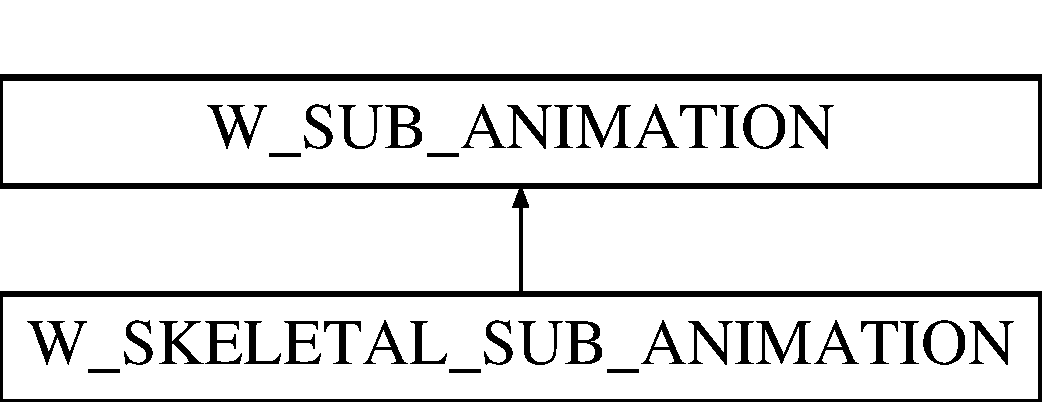
\includegraphics[height=2.000000cm]{struct_w___s_u_b___a_n_i_m_a_t_i_o_n}
\end{center}
\end{figure}
\subsection*{Public Attributes}
\begin{DoxyCompactItemize}
\item 
unsigned int \hyperlink{struct_w___s_u_b___a_n_i_m_a_t_i_o_n_a6eaba4aaaf7dad81d0259fdfb5b0ee84}{cur\+Frame}
\item 
unsigned int \hyperlink{struct_w___s_u_b___a_n_i_m_a_t_i_o_n_a4c308bafa17ea951fcf4486caf9f45b8}{next\+Frame}
\item 
unsigned int \hyperlink{struct_w___s_u_b___a_n_i_m_a_t_i_o_n_a32f726d022afd30cff9b7cae9259cafa}{first\+Frame}
\item 
bool \hyperlink{struct_w___s_u_b___a_n_i_m_a_t_i_o_n_a8cf7c188213a51cd0bf3a2bb18add32b}{b\+Playing}
\item 
bool \hyperlink{struct_w___s_u_b___a_n_i_m_a_t_i_o_n_ae3af9aac28fa44b1c27f8834fa47371d}{b\+Loop}
\item 
float \hyperlink{struct_w___s_u_b___a_n_i_m_a_t_i_o_n_ae6866df11b272a2a1928d54165ef2824}{f\+Current\+Time}
\item 
float \hyperlink{struct_w___s_u_b___a_n_i_m_a_t_i_o_n_a5f1a892565c32d4d6da2a98d209ce2a5}{f\+Speed}
\item 
float \hyperlink{struct_w___s_u_b___a_n_i_m_a_t_i_o_n_a34791417cc32bb2ddbe3f9d421e74d2d}{f\+Play\+Start\+Time}
\item 
float \hyperlink{struct_w___s_u_b___a_n_i_m_a_t_i_o_n_aab134456793deb3cd3b1f0689f3617ef}{f\+Play\+End\+Time}
\end{DoxyCompactItemize}


\subsection{Detailed Description}
Represents a subanimation. 

\subsection{Member Data Documentation}
\index{W\+\_\+\+S\+U\+B\+\_\+\+A\+N\+I\+M\+A\+T\+I\+ON@{W\+\_\+\+S\+U\+B\+\_\+\+A\+N\+I\+M\+A\+T\+I\+ON}!b\+Loop@{b\+Loop}}
\index{b\+Loop@{b\+Loop}!W\+\_\+\+S\+U\+B\+\_\+\+A\+N\+I\+M\+A\+T\+I\+ON@{W\+\_\+\+S\+U\+B\+\_\+\+A\+N\+I\+M\+A\+T\+I\+ON}}
\subsubsection[{\texorpdfstring{b\+Loop}{bLoop}}]{\setlength{\rightskip}{0pt plus 5cm}bool W\+\_\+\+S\+U\+B\+\_\+\+A\+N\+I\+M\+A\+T\+I\+O\+N\+::b\+Loop}\hypertarget{struct_w___s_u_b___a_n_i_m_a_t_i_o_n_ae3af9aac28fa44b1c27f8834fa47371d}{}\label{struct_w___s_u_b___a_n_i_m_a_t_i_o_n_ae3af9aac28fa44b1c27f8834fa47371d}
true if the animation is looping. \index{W\+\_\+\+S\+U\+B\+\_\+\+A\+N\+I\+M\+A\+T\+I\+ON@{W\+\_\+\+S\+U\+B\+\_\+\+A\+N\+I\+M\+A\+T\+I\+ON}!b\+Playing@{b\+Playing}}
\index{b\+Playing@{b\+Playing}!W\+\_\+\+S\+U\+B\+\_\+\+A\+N\+I\+M\+A\+T\+I\+ON@{W\+\_\+\+S\+U\+B\+\_\+\+A\+N\+I\+M\+A\+T\+I\+ON}}
\subsubsection[{\texorpdfstring{b\+Playing}{bPlaying}}]{\setlength{\rightskip}{0pt plus 5cm}bool W\+\_\+\+S\+U\+B\+\_\+\+A\+N\+I\+M\+A\+T\+I\+O\+N\+::b\+Playing}\hypertarget{struct_w___s_u_b___a_n_i_m_a_t_i_o_n_a8cf7c188213a51cd0bf3a2bb18add32b}{}\label{struct_w___s_u_b___a_n_i_m_a_t_i_o_n_a8cf7c188213a51cd0bf3a2bb18add32b}
true if the subanimation is playing (or looping). \index{W\+\_\+\+S\+U\+B\+\_\+\+A\+N\+I\+M\+A\+T\+I\+ON@{W\+\_\+\+S\+U\+B\+\_\+\+A\+N\+I\+M\+A\+T\+I\+ON}!cur\+Frame@{cur\+Frame}}
\index{cur\+Frame@{cur\+Frame}!W\+\_\+\+S\+U\+B\+\_\+\+A\+N\+I\+M\+A\+T\+I\+ON@{W\+\_\+\+S\+U\+B\+\_\+\+A\+N\+I\+M\+A\+T\+I\+ON}}
\subsubsection[{\texorpdfstring{cur\+Frame}{curFrame}}]{\setlength{\rightskip}{0pt plus 5cm}unsigned int W\+\_\+\+S\+U\+B\+\_\+\+A\+N\+I\+M\+A\+T\+I\+O\+N\+::cur\+Frame}\hypertarget{struct_w___s_u_b___a_n_i_m_a_t_i_o_n_a6eaba4aaaf7dad81d0259fdfb5b0ee84}{}\label{struct_w___s_u_b___a_n_i_m_a_t_i_o_n_a6eaba4aaaf7dad81d0259fdfb5b0ee84}
The frame this subanimation is currently in. \index{W\+\_\+\+S\+U\+B\+\_\+\+A\+N\+I\+M\+A\+T\+I\+ON@{W\+\_\+\+S\+U\+B\+\_\+\+A\+N\+I\+M\+A\+T\+I\+ON}!f\+Current\+Time@{f\+Current\+Time}}
\index{f\+Current\+Time@{f\+Current\+Time}!W\+\_\+\+S\+U\+B\+\_\+\+A\+N\+I\+M\+A\+T\+I\+ON@{W\+\_\+\+S\+U\+B\+\_\+\+A\+N\+I\+M\+A\+T\+I\+ON}}
\subsubsection[{\texorpdfstring{f\+Current\+Time}{fCurrentTime}}]{\setlength{\rightskip}{0pt plus 5cm}float W\+\_\+\+S\+U\+B\+\_\+\+A\+N\+I\+M\+A\+T\+I\+O\+N\+::f\+Current\+Time}\hypertarget{struct_w___s_u_b___a_n_i_m_a_t_i_o_n_ae6866df11b272a2a1928d54165ef2824}{}\label{struct_w___s_u_b___a_n_i_m_a_t_i_o_n_ae6866df11b272a2a1928d54165ef2824}
The current time in the subanimation. \index{W\+\_\+\+S\+U\+B\+\_\+\+A\+N\+I\+M\+A\+T\+I\+ON@{W\+\_\+\+S\+U\+B\+\_\+\+A\+N\+I\+M\+A\+T\+I\+ON}!first\+Frame@{first\+Frame}}
\index{first\+Frame@{first\+Frame}!W\+\_\+\+S\+U\+B\+\_\+\+A\+N\+I\+M\+A\+T\+I\+ON@{W\+\_\+\+S\+U\+B\+\_\+\+A\+N\+I\+M\+A\+T\+I\+ON}}
\subsubsection[{\texorpdfstring{first\+Frame}{firstFrame}}]{\setlength{\rightskip}{0pt plus 5cm}unsigned int W\+\_\+\+S\+U\+B\+\_\+\+A\+N\+I\+M\+A\+T\+I\+O\+N\+::first\+Frame}\hypertarget{struct_w___s_u_b___a_n_i_m_a_t_i_o_n_a32f726d022afd30cff9b7cae9259cafa}{}\label{struct_w___s_u_b___a_n_i_m_a_t_i_o_n_a32f726d022afd30cff9b7cae9259cafa}
The first frame within the play boundaries. \index{W\+\_\+\+S\+U\+B\+\_\+\+A\+N\+I\+M\+A\+T\+I\+ON@{W\+\_\+\+S\+U\+B\+\_\+\+A\+N\+I\+M\+A\+T\+I\+ON}!f\+Play\+End\+Time@{f\+Play\+End\+Time}}
\index{f\+Play\+End\+Time@{f\+Play\+End\+Time}!W\+\_\+\+S\+U\+B\+\_\+\+A\+N\+I\+M\+A\+T\+I\+ON@{W\+\_\+\+S\+U\+B\+\_\+\+A\+N\+I\+M\+A\+T\+I\+ON}}
\subsubsection[{\texorpdfstring{f\+Play\+End\+Time}{fPlayEndTime}}]{\setlength{\rightskip}{0pt plus 5cm}float W\+\_\+\+S\+U\+B\+\_\+\+A\+N\+I\+M\+A\+T\+I\+O\+N\+::f\+Play\+End\+Time}\hypertarget{struct_w___s_u_b___a_n_i_m_a_t_i_o_n_aab134456793deb3cd3b1f0689f3617ef}{}\label{struct_w___s_u_b___a_n_i_m_a_t_i_o_n_aab134456793deb3cd3b1f0689f3617ef}
Ending time for the play boundaries. \index{W\+\_\+\+S\+U\+B\+\_\+\+A\+N\+I\+M\+A\+T\+I\+ON@{W\+\_\+\+S\+U\+B\+\_\+\+A\+N\+I\+M\+A\+T\+I\+ON}!f\+Play\+Start\+Time@{f\+Play\+Start\+Time}}
\index{f\+Play\+Start\+Time@{f\+Play\+Start\+Time}!W\+\_\+\+S\+U\+B\+\_\+\+A\+N\+I\+M\+A\+T\+I\+ON@{W\+\_\+\+S\+U\+B\+\_\+\+A\+N\+I\+M\+A\+T\+I\+ON}}
\subsubsection[{\texorpdfstring{f\+Play\+Start\+Time}{fPlayStartTime}}]{\setlength{\rightskip}{0pt plus 5cm}float W\+\_\+\+S\+U\+B\+\_\+\+A\+N\+I\+M\+A\+T\+I\+O\+N\+::f\+Play\+Start\+Time}\hypertarget{struct_w___s_u_b___a_n_i_m_a_t_i_o_n_a34791417cc32bb2ddbe3f9d421e74d2d}{}\label{struct_w___s_u_b___a_n_i_m_a_t_i_o_n_a34791417cc32bb2ddbe3f9d421e74d2d}
Starting time for the play boundaries. \index{W\+\_\+\+S\+U\+B\+\_\+\+A\+N\+I\+M\+A\+T\+I\+ON@{W\+\_\+\+S\+U\+B\+\_\+\+A\+N\+I\+M\+A\+T\+I\+ON}!f\+Speed@{f\+Speed}}
\index{f\+Speed@{f\+Speed}!W\+\_\+\+S\+U\+B\+\_\+\+A\+N\+I\+M\+A\+T\+I\+ON@{W\+\_\+\+S\+U\+B\+\_\+\+A\+N\+I\+M\+A\+T\+I\+ON}}
\subsubsection[{\texorpdfstring{f\+Speed}{fSpeed}}]{\setlength{\rightskip}{0pt plus 5cm}float W\+\_\+\+S\+U\+B\+\_\+\+A\+N\+I\+M\+A\+T\+I\+O\+N\+::f\+Speed}\hypertarget{struct_w___s_u_b___a_n_i_m_a_t_i_o_n_a5f1a892565c32d4d6da2a98d209ce2a5}{}\label{struct_w___s_u_b___a_n_i_m_a_t_i_o_n_a5f1a892565c32d4d6da2a98d209ce2a5}
The speed multiplier for the subanimation. \index{W\+\_\+\+S\+U\+B\+\_\+\+A\+N\+I\+M\+A\+T\+I\+ON@{W\+\_\+\+S\+U\+B\+\_\+\+A\+N\+I\+M\+A\+T\+I\+ON}!next\+Frame@{next\+Frame}}
\index{next\+Frame@{next\+Frame}!W\+\_\+\+S\+U\+B\+\_\+\+A\+N\+I\+M\+A\+T\+I\+ON@{W\+\_\+\+S\+U\+B\+\_\+\+A\+N\+I\+M\+A\+T\+I\+ON}}
\subsubsection[{\texorpdfstring{next\+Frame}{nextFrame}}]{\setlength{\rightskip}{0pt plus 5cm}unsigned int W\+\_\+\+S\+U\+B\+\_\+\+A\+N\+I\+M\+A\+T\+I\+O\+N\+::next\+Frame}\hypertarget{struct_w___s_u_b___a_n_i_m_a_t_i_o_n_a4c308bafa17ea951fcf4486caf9f45b8}{}\label{struct_w___s_u_b___a_n_i_m_a_t_i_o_n_a4c308bafa17ea951fcf4486caf9f45b8}
The next frame this subanimation is merging to. 

The documentation for this struct was generated from the following file\+:\begin{DoxyCompactItemize}
\item 
Wasabi/\+Animations/\hyperlink{_w_animation_8h}{W\+Animation.\+h}\end{DoxyCompactItemize}

\hypertarget{struct_w___v_e_r_t_e_x___a_t_t_r_i_b_u_t_e}{}\section{W\+\_\+\+V\+E\+R\+T\+E\+X\+\_\+\+A\+T\+T\+R\+I\+B\+U\+TE Struct Reference}
\label{struct_w___v_e_r_t_e_x___a_t_t_r_i_b_u_t_e}\index{W\+\_\+\+V\+E\+R\+T\+E\+X\+\_\+\+A\+T\+T\+R\+I\+B\+U\+TE@{W\+\_\+\+V\+E\+R\+T\+E\+X\+\_\+\+A\+T\+T\+R\+I\+B\+U\+TE}}


{\ttfamily \#include $<$W\+Geometry.\+h$>$}

\subsection*{Public Member Functions}
\begin{DoxyCompactItemize}
\item 
{\bfseries W\+\_\+\+V\+E\+R\+T\+E\+X\+\_\+\+A\+T\+T\+R\+I\+B\+U\+TE} (std\+::string n, unsigned char s)\hypertarget{struct_w___v_e_r_t_e_x___a_t_t_r_i_b_u_t_e_af482c26336e8575553f70e125919224d}{}\label{struct_w___v_e_r_t_e_x___a_t_t_r_i_b_u_t_e_af482c26336e8575553f70e125919224d}

\end{DoxyCompactItemize}
\subsection*{Public Attributes}
\begin{DoxyCompactItemize}
\item 
std\+::string \hyperlink{struct_w___v_e_r_t_e_x___a_t_t_r_i_b_u_t_e_a428e56ded0a3989a627db00fc59613c8}{name}
\item 
unsigned char \hyperlink{struct_w___v_e_r_t_e_x___a_t_t_r_i_b_u_t_e_a79739d8644e1aa585131fc54648cd047}{num\+\_\+components}
\end{DoxyCompactItemize}


\subsection{Detailed Description}
Represents a single vertex attribute. 

\subsection{Member Data Documentation}
\index{W\+\_\+\+V\+E\+R\+T\+E\+X\+\_\+\+A\+T\+T\+R\+I\+B\+U\+TE@{W\+\_\+\+V\+E\+R\+T\+E\+X\+\_\+\+A\+T\+T\+R\+I\+B\+U\+TE}!name@{name}}
\index{name@{name}!W\+\_\+\+V\+E\+R\+T\+E\+X\+\_\+\+A\+T\+T\+R\+I\+B\+U\+TE@{W\+\_\+\+V\+E\+R\+T\+E\+X\+\_\+\+A\+T\+T\+R\+I\+B\+U\+TE}}
\subsubsection[{\texorpdfstring{name}{name}}]{\setlength{\rightskip}{0pt plus 5cm}std\+::string W\+\_\+\+V\+E\+R\+T\+E\+X\+\_\+\+A\+T\+T\+R\+I\+B\+U\+T\+E\+::name}\hypertarget{struct_w___v_e_r_t_e_x___a_t_t_r_i_b_u_t_e_a428e56ded0a3989a627db00fc59613c8}{}\label{struct_w___v_e_r_t_e_x___a_t_t_r_i_b_u_t_e_a428e56ded0a3989a627db00fc59613c8}
Attribute name \index{W\+\_\+\+V\+E\+R\+T\+E\+X\+\_\+\+A\+T\+T\+R\+I\+B\+U\+TE@{W\+\_\+\+V\+E\+R\+T\+E\+X\+\_\+\+A\+T\+T\+R\+I\+B\+U\+TE}!num\+\_\+components@{num\+\_\+components}}
\index{num\+\_\+components@{num\+\_\+components}!W\+\_\+\+V\+E\+R\+T\+E\+X\+\_\+\+A\+T\+T\+R\+I\+B\+U\+TE@{W\+\_\+\+V\+E\+R\+T\+E\+X\+\_\+\+A\+T\+T\+R\+I\+B\+U\+TE}}
\subsubsection[{\texorpdfstring{num\+\_\+components}{num_components}}]{\setlength{\rightskip}{0pt plus 5cm}unsigned char W\+\_\+\+V\+E\+R\+T\+E\+X\+\_\+\+A\+T\+T\+R\+I\+B\+U\+T\+E\+::num\+\_\+components}\hypertarget{struct_w___v_e_r_t_e_x___a_t_t_r_i_b_u_t_e_a79739d8644e1aa585131fc54648cd047}{}\label{struct_w___v_e_r_t_e_x___a_t_t_r_i_b_u_t_e_a79739d8644e1aa585131fc54648cd047}
Number of components of the attribute 

The documentation for this struct was generated from the following file\+:\begin{DoxyCompactItemize}
\item 
Wasabi/\+Geometries/\hyperlink{_w_geometry_8h}{W\+Geometry.\+h}\end{DoxyCompactItemize}

\hypertarget{struct_w___v_e_r_t_e_x___d_e_s_c_r_i_p_t_i_o_n}{}\section{W\+\_\+\+V\+E\+R\+T\+E\+X\+\_\+\+D\+E\+S\+C\+R\+I\+P\+T\+I\+ON Struct Reference}
\label{struct_w___v_e_r_t_e_x___d_e_s_c_r_i_p_t_i_o_n}\index{W\+\_\+\+V\+E\+R\+T\+E\+X\+\_\+\+D\+E\+S\+C\+R\+I\+P\+T\+I\+ON@{W\+\_\+\+V\+E\+R\+T\+E\+X\+\_\+\+D\+E\+S\+C\+R\+I\+P\+T\+I\+ON}}


{\ttfamily \#include $<$W\+Geometry.\+h$>$}

\subsection*{Public Member Functions}
\begin{DoxyCompactItemize}
\item 
{\bfseries W\+\_\+\+V\+E\+R\+T\+E\+X\+\_\+\+D\+E\+S\+C\+R\+I\+P\+T\+I\+ON} (std\+::vector$<$ \hyperlink{struct_w___v_e_r_t_e_x___a_t_t_r_i_b_u_t_e}{W\+\_\+\+V\+E\+R\+T\+E\+X\+\_\+\+A\+T\+T\+R\+I\+B\+U\+TE} $>$ attribs=\{\})\hypertarget{struct_w___v_e_r_t_e_x___d_e_s_c_r_i_p_t_i_o_n_a333f0377b3556311a11edda7c4e18a8b}{}\label{struct_w___v_e_r_t_e_x___d_e_s_c_r_i_p_t_i_o_n_a333f0377b3556311a11edda7c4e18a8b}

\item 
size\+\_\+t \hyperlink{struct_w___v_e_r_t_e_x___d_e_s_c_r_i_p_t_i_o_n_a7c06d9c07ee2fdd4d47c06592e79158e}{Get\+Size} () const 
\item 
size\+\_\+t \hyperlink{struct_w___v_e_r_t_e_x___d_e_s_c_r_i_p_t_i_o_n_a06aea062550c1ce607bc3dbffebaa74f}{Get\+Offset} (unsigned int attrib\+\_\+index) const 
\item 
size\+\_\+t \hyperlink{struct_w___v_e_r_t_e_x___d_e_s_c_r_i_p_t_i_o_n_a541b178fbbf15c4166c51d59f377994d}{Get\+Offset} (std\+::string attrib\+\_\+name) const 
\item 
unsigned int \hyperlink{struct_w___v_e_r_t_e_x___d_e_s_c_r_i_p_t_i_o_n_a981ce484b325b9cb8380076d8b21dbd8}{Get\+Index} (std\+::string attrib\+\_\+name) const 
\end{DoxyCompactItemize}
\subsection*{Public Attributes}
\begin{DoxyCompactItemize}
\item 
std\+::vector$<$ \hyperlink{struct_w___v_e_r_t_e_x___a_t_t_r_i_b_u_t_e}{W\+\_\+\+V\+E\+R\+T\+E\+X\+\_\+\+A\+T\+T\+R\+I\+B\+U\+TE} $>$ \hyperlink{struct_w___v_e_r_t_e_x___d_e_s_c_r_i_p_t_i_o_n_a559e7d9127c860535a58ba6217fb7fd5}{attributes}
\end{DoxyCompactItemize}


\subsection{Detailed Description}
Represents the description of a vertex. A vertex is described by a list of its attributes. 

\subsection{Member Function Documentation}
\index{W\+\_\+\+V\+E\+R\+T\+E\+X\+\_\+\+D\+E\+S\+C\+R\+I\+P\+T\+I\+ON@{W\+\_\+\+V\+E\+R\+T\+E\+X\+\_\+\+D\+E\+S\+C\+R\+I\+P\+T\+I\+ON}!Get\+Index@{Get\+Index}}
\index{Get\+Index@{Get\+Index}!W\+\_\+\+V\+E\+R\+T\+E\+X\+\_\+\+D\+E\+S\+C\+R\+I\+P\+T\+I\+ON@{W\+\_\+\+V\+E\+R\+T\+E\+X\+\_\+\+D\+E\+S\+C\+R\+I\+P\+T\+I\+ON}}
\subsubsection[{\texorpdfstring{Get\+Index(std\+::string attrib\+\_\+name) const }{GetIndex(std::string attrib_name) const }}]{\setlength{\rightskip}{0pt plus 5cm}unsigned int W\+\_\+\+V\+E\+R\+T\+E\+X\+\_\+\+D\+E\+S\+C\+R\+I\+P\+T\+I\+O\+N\+::\+Get\+Index (
\begin{DoxyParamCaption}
\item[{std\+::string}]{attrib\+\_\+name}
\end{DoxyParamCaption}
) const}\hypertarget{struct_w___v_e_r_t_e_x___d_e_s_c_r_i_p_t_i_o_n_a981ce484b325b9cb8380076d8b21dbd8}{}\label{struct_w___v_e_r_t_e_x___d_e_s_c_r_i_p_t_i_o_n_a981ce484b325b9cb8380076d8b21dbd8}
Find the index of an attribute given its name. 
\begin{DoxyParams}{Parameters}
{\em attrib\+\_\+name} & Attribute name to look for \\
\hline
\end{DoxyParams}
\begin{DoxyReturn}{Returns}
Index of the attribute whose name is attrib\+\_\+name, -\/1 if it cannot be found 
\end{DoxyReturn}
\index{W\+\_\+\+V\+E\+R\+T\+E\+X\+\_\+\+D\+E\+S\+C\+R\+I\+P\+T\+I\+ON@{W\+\_\+\+V\+E\+R\+T\+E\+X\+\_\+\+D\+E\+S\+C\+R\+I\+P\+T\+I\+ON}!Get\+Offset@{Get\+Offset}}
\index{Get\+Offset@{Get\+Offset}!W\+\_\+\+V\+E\+R\+T\+E\+X\+\_\+\+D\+E\+S\+C\+R\+I\+P\+T\+I\+ON@{W\+\_\+\+V\+E\+R\+T\+E\+X\+\_\+\+D\+E\+S\+C\+R\+I\+P\+T\+I\+ON}}
\subsubsection[{\texorpdfstring{Get\+Offset(unsigned int attrib\+\_\+index) const }{GetOffset(unsigned int attrib_index) const }}]{\setlength{\rightskip}{0pt plus 5cm}size\+\_\+t W\+\_\+\+V\+E\+R\+T\+E\+X\+\_\+\+D\+E\+S\+C\+R\+I\+P\+T\+I\+O\+N\+::\+Get\+Offset (
\begin{DoxyParamCaption}
\item[{unsigned int}]{attrib\+\_\+index}
\end{DoxyParamCaption}
) const}\hypertarget{struct_w___v_e_r_t_e_x___d_e_s_c_r_i_p_t_i_o_n_a06aea062550c1ce607bc3dbffebaa74f}{}\label{struct_w___v_e_r_t_e_x___d_e_s_c_r_i_p_t_i_o_n_a06aea062550c1ce607bc3dbffebaa74f}
Retrieves the offset (in bytes) to a certain attribute. 
\begin{DoxyParams}{Parameters}
{\em attrib\+\_\+index} & Index of the attribute to get its offset \\
\hline
\end{DoxyParams}
\begin{DoxyReturn}{Returns}
The offset of the attribute at attrib\+\_\+index 
\end{DoxyReturn}
\index{W\+\_\+\+V\+E\+R\+T\+E\+X\+\_\+\+D\+E\+S\+C\+R\+I\+P\+T\+I\+ON@{W\+\_\+\+V\+E\+R\+T\+E\+X\+\_\+\+D\+E\+S\+C\+R\+I\+P\+T\+I\+ON}!Get\+Offset@{Get\+Offset}}
\index{Get\+Offset@{Get\+Offset}!W\+\_\+\+V\+E\+R\+T\+E\+X\+\_\+\+D\+E\+S\+C\+R\+I\+P\+T\+I\+ON@{W\+\_\+\+V\+E\+R\+T\+E\+X\+\_\+\+D\+E\+S\+C\+R\+I\+P\+T\+I\+ON}}
\subsubsection[{\texorpdfstring{Get\+Offset(std\+::string attrib\+\_\+name) const }{GetOffset(std::string attrib_name) const }}]{\setlength{\rightskip}{0pt plus 5cm}size\+\_\+t W\+\_\+\+V\+E\+R\+T\+E\+X\+\_\+\+D\+E\+S\+C\+R\+I\+P\+T\+I\+O\+N\+::\+Get\+Offset (
\begin{DoxyParamCaption}
\item[{std\+::string}]{attrib\+\_\+name}
\end{DoxyParamCaption}
) const}\hypertarget{struct_w___v_e_r_t_e_x___d_e_s_c_r_i_p_t_i_o_n_a541b178fbbf15c4166c51d59f377994d}{}\label{struct_w___v_e_r_t_e_x___d_e_s_c_r_i_p_t_i_o_n_a541b178fbbf15c4166c51d59f377994d}
Retrieves the offset (in bytes) to a certain attribute. 
\begin{DoxyParams}{Parameters}
{\em attrib\+\_\+name} & Name of the attribute to get its offset \\
\hline
\end{DoxyParams}
\begin{DoxyReturn}{Returns}
The offset of the attribute at attrib\+\_\+index 
\end{DoxyReturn}
\index{W\+\_\+\+V\+E\+R\+T\+E\+X\+\_\+\+D\+E\+S\+C\+R\+I\+P\+T\+I\+ON@{W\+\_\+\+V\+E\+R\+T\+E\+X\+\_\+\+D\+E\+S\+C\+R\+I\+P\+T\+I\+ON}!Get\+Size@{Get\+Size}}
\index{Get\+Size@{Get\+Size}!W\+\_\+\+V\+E\+R\+T\+E\+X\+\_\+\+D\+E\+S\+C\+R\+I\+P\+T\+I\+ON@{W\+\_\+\+V\+E\+R\+T\+E\+X\+\_\+\+D\+E\+S\+C\+R\+I\+P\+T\+I\+ON}}
\subsubsection[{\texorpdfstring{Get\+Size() const }{GetSize() const }}]{\setlength{\rightskip}{0pt plus 5cm}size\+\_\+t W\+\_\+\+V\+E\+R\+T\+E\+X\+\_\+\+D\+E\+S\+C\+R\+I\+P\+T\+I\+O\+N\+::\+Get\+Size (
\begin{DoxyParamCaption}
{}
\end{DoxyParamCaption}
) const}\hypertarget{struct_w___v_e_r_t_e_x___d_e_s_c_r_i_p_t_i_o_n_a7c06d9c07ee2fdd4d47c06592e79158e}{}\label{struct_w___v_e_r_t_e_x___d_e_s_c_r_i_p_t_i_o_n_a7c06d9c07ee2fdd4d47c06592e79158e}
Retrieves the size (in bytes) of a vertex of this description. \begin{DoxyReturn}{Returns}
Size (in bytes) of a vertex of this description 
\end{DoxyReturn}


\subsection{Member Data Documentation}
\index{W\+\_\+\+V\+E\+R\+T\+E\+X\+\_\+\+D\+E\+S\+C\+R\+I\+P\+T\+I\+ON@{W\+\_\+\+V\+E\+R\+T\+E\+X\+\_\+\+D\+E\+S\+C\+R\+I\+P\+T\+I\+ON}!attributes@{attributes}}
\index{attributes@{attributes}!W\+\_\+\+V\+E\+R\+T\+E\+X\+\_\+\+D\+E\+S\+C\+R\+I\+P\+T\+I\+ON@{W\+\_\+\+V\+E\+R\+T\+E\+X\+\_\+\+D\+E\+S\+C\+R\+I\+P\+T\+I\+ON}}
\subsubsection[{\texorpdfstring{attributes}{attributes}}]{\setlength{\rightskip}{0pt plus 5cm}std\+::vector$<${\bf W\+\_\+\+V\+E\+R\+T\+E\+X\+\_\+\+A\+T\+T\+R\+I\+B\+U\+TE}$>$ W\+\_\+\+V\+E\+R\+T\+E\+X\+\_\+\+D\+E\+S\+C\+R\+I\+P\+T\+I\+O\+N\+::attributes}\hypertarget{struct_w___v_e_r_t_e_x___d_e_s_c_r_i_p_t_i_o_n_a559e7d9127c860535a58ba6217fb7fd5}{}\label{struct_w___v_e_r_t_e_x___d_e_s_c_r_i_p_t_i_o_n_a559e7d9127c860535a58ba6217fb7fd5}
A list of attributes for the vertex 

The documentation for this struct was generated from the following files\+:\begin{DoxyCompactItemize}
\item 
Wasabi/\+Geometries/\hyperlink{_w_geometry_8h}{W\+Geometry.\+h}\item 
Wasabi/\+Geometries/W\+Geometry.\+cpp\end{DoxyCompactItemize}

\hypertarget{class_w_animation}{}\section{W\+Animation Class Reference}
\label{class_w_animation}\index{W\+Animation@{W\+Animation}}


{\ttfamily \#include $<$W\+Animation.\+h$>$}

Inheritance diagram for W\+Animation\+:\begin{figure}[H]
\begin{center}
\leavevmode
\includegraphics[height=3.000000cm]{class_w_animation}
\end{center}
\end{figure}
\subsection*{Public Member Functions}
\begin{DoxyCompactItemize}
\item 
{\bfseries W\+Animation} (class \hyperlink{class_wasabi}{Wasabi} $\ast$const app, unsigned int ID=0)\hypertarget{class_w_animation_ae96f0fbf2bb9d6d362d400056297a2a6}{}\label{class_w_animation_ae96f0fbf2bb9d6d362d400056297a2a6}

\item 
virtual void \hyperlink{class_w_animation_a14390c833c0f255fcb461661f0577c6e}{Update} (float f\+Delta\+Time)
\item 
virtual class \hyperlink{class_w_image}{W\+Image} $\ast$ \hyperlink{class_w_animation_a6d7a8cbd7db22b88c528c7ed2c61601f}{Get\+Texture} () const  =0
\item 
virtual void \hyperlink{class_w_animation_a42f0459e88ccf7e2c6414a9512865c6f}{Add\+Sub\+Animation} ()
\item 
virtual void \hyperlink{class_w_animation_ad5e5118abd61cbbc91b9b28ef0d6481b}{Remove\+Sub\+Animation} (unsigned int index)
\item 
\hyperlink{class_w_error}{W\+Error} \hyperlink{class_w_animation_a2dfe828c0ae005378bb267d55044cdbd}{Set\+Key\+Frame\+Time} (unsigned int frame, float f\+Time)
\item 
void \hyperlink{class_w_animation_ac9a3edc475eb5be9ee7ef56f717a30d4}{Set\+Play\+Speed} (float f\+Speed\+Multiplier, unsigned int sub\+Animation=-\/1)
\item 
void \hyperlink{class_w_animation_a4b4ef4c57105cad41308da11b2329bcc}{Set\+Current\+Frame} (unsigned int frame, unsigned int sub\+Animation=0)
\item 
void \hyperlink{class_w_animation_ab3784a49233c2683ff3ee6c40b92a307}{Set\+Current\+Time} (float f\+Time, unsigned int sub\+Animation=0)
\item 
void \hyperlink{class_w_animation_a74ee2ca45a4b268d944f4507354389bd}{Set\+Playing\+Bounds} (unsigned int start\+Frame, unsigned int end\+Frame, unsigned int sub\+Animation=0)
\item 
void \hyperlink{class_w_animation_a6b47183956a92e3da0526538d1b5105e}{Set\+Playing\+Bounds\+\_\+\+Time} (float f\+Start\+Time, float f\+End\+Time, unsigned int sub\+Animation=0)
\item 
void \hyperlink{class_w_animation_a9aea2f7128ee0235457852f06d0e4edc}{Play} (unsigned int sub\+Animation=-\/1)
\item 
void \hyperlink{class_w_animation_a559fff86972e7cf44a744f8078bebe56}{Loop} (unsigned int sub\+Animation=-\/1)
\item 
void \hyperlink{class_w_animation_a1bcf0c8298ffa440df1a3332008997a8}{Stop} (unsigned int sub\+Animation=-\/1)
\item 
void \hyperlink{class_w_animation_aa80c5c55a56dac19b1ee9f14d4f4e864}{Reset} (unsigned int sub\+Animation=-\/1)
\item 
bool \hyperlink{class_w_animation_a45eb95970e48cfb50657e5b551afb66a}{Playing} (unsigned int sub\+Animation=0) const 
\item 
bool \hyperlink{class_w_animation_a0491a2e346bd3288dc25dacea32ce3a7}{Looping} (unsigned int sub\+Animation=0) const 
\item 
float \hyperlink{class_w_animation_a9bdbde4087f3752e8178e606aeda5d42}{Get\+Time} (unsigned int sub\+Animation=0) const 
\item 
virtual \hyperlink{class_w_error}{W\+Error} \hyperlink{class_w_animation_a011a53c9674f21c34f86883cefef3ad3}{Load\+From\+WA} (std\+::string Filename)=0
\item 
virtual \hyperlink{class_w_error}{W\+Error} \hyperlink{class_w_animation_a85ef267b11ef54ac9a2a4beba53eb1d4}{Load\+From\+WA} (basic\+\_\+filebuf$<$ char $>$ $\ast$buff=nullptr, unsigned int pos=0)=0
\item 
virtual \hyperlink{class_w_error}{W\+Error} \hyperlink{class_w_animation_a0cac916766d0ad9ec50621a365518536}{Save\+To\+WA} (basic\+\_\+filebuf$<$ char $>$ $\ast$buff=nullptr, unsigned int pos=0) const  =0
\item 
virtual \hyperlink{class_w_error}{W\+Error} \hyperlink{class_w_animation_aa9d5d21f13a215a7ccf2432a3d9aeef0}{Save\+To\+WA} (std\+::string Filename) const  =0
\item 
virtual \hyperlink{class_w_error}{W\+Error} \hyperlink{class_w_animation_a42ee18109b6a417733c81d513f82184d}{Copy\+From} (const \hyperlink{class_w_animation}{W\+Animation} $\ast$const from)=0
\item 
virtual \hyperlink{class_w_error}{W\+Error} \hyperlink{class_w_animation_af341efba3efd68107679396c2e31839d}{Use\+Animation\+Frames} (const \hyperlink{class_w_animation}{W\+Animation} $\ast$const anim)=0
\end{DoxyCompactItemize}
\subsection*{Protected Member Functions}
\begin{DoxyCompactItemize}
\item 
void \hyperlink{class_w_animation_a6bf60a7c40631e99b88a8a8cb1ea88e8}{m\+\_\+\+Update\+First\+Frame} (unsigned int sub\+Animation=-\/1)
\end{DoxyCompactItemize}
\subsection*{Protected Attributes}
\begin{DoxyCompactItemize}
\item 
bool \hyperlink{class_w_animation_a2aca672278527eed1f5477690a3f1a9e}{m\+\_\+b\+Frames\+Owner}
\item 
float \hyperlink{class_w_animation_a0a819e66ae3c7aed6fae97482c3a8281}{m\+\_\+total\+Time}
\item 
vector$<$ \hyperlink{struct_w___f_r_a_m_e}{W\+\_\+\+F\+R\+A\+ME} $\ast$ $>$ \hyperlink{class_w_animation_adee42ca012501f00569e58277a5bf708}{m\+\_\+frames}
\item 
vector$<$ \hyperlink{struct_w___s_u_b___a_n_i_m_a_t_i_o_n}{W\+\_\+\+S\+U\+B\+\_\+\+A\+N\+I\+M\+A\+T\+I\+ON} $\ast$ $>$ \hyperlink{class_w_animation_ac8bd5b9f5b8ddae1a8658a169e0cbf51}{m\+\_\+sub\+Animations}
\end{DoxyCompactItemize}


\subsection{Detailed Description}
This is an abstract base class that represents an animation which could be attached to an object. This base class is responsible for maintaining subanimations and managing their playing and looping. 

\subsection{Member Function Documentation}
\index{W\+Animation@{W\+Animation}!Add\+Sub\+Animation@{Add\+Sub\+Animation}}
\index{Add\+Sub\+Animation@{Add\+Sub\+Animation}!W\+Animation@{W\+Animation}}
\subsubsection[{\texorpdfstring{Add\+Sub\+Animation()}{AddSubAnimation()}}]{\setlength{\rightskip}{0pt plus 5cm}void W\+Animation\+::\+Add\+Sub\+Animation (
\begin{DoxyParamCaption}
{}
\end{DoxyParamCaption}
)\hspace{0.3cm}{\ttfamily [virtual]}}\hypertarget{class_w_animation_a42f0459e88ccf7e2c6414a9512865c6f}{}\label{class_w_animation_a42f0459e88ccf7e2c6414a9512865c6f}
Appends a subanimation to this animation. 

Reimplemented in \hyperlink{class_w_skeleton_af8de1fd3b0d620873ae0341058441d9a}{W\+Skeleton}.

\index{W\+Animation@{W\+Animation}!Copy\+From@{Copy\+From}}
\index{Copy\+From@{Copy\+From}!W\+Animation@{W\+Animation}}
\subsubsection[{\texorpdfstring{Copy\+From(const W\+Animation $\ast$const from)=0}{CopyFrom(const WAnimation *const from)=0}}]{\setlength{\rightskip}{0pt plus 5cm}virtual {\bf W\+Error} W\+Animation\+::\+Copy\+From (
\begin{DoxyParamCaption}
\item[{const {\bf W\+Animation} $\ast$const}]{from}
\end{DoxyParamCaption}
)\hspace{0.3cm}{\ttfamily [pure virtual]}}\hypertarget{class_w_animation_a42ee18109b6a417733c81d513f82184d}{}\label{class_w_animation_a42ee18109b6a417733c81d513f82184d}
Copies another \hyperlink{class_w_animation}{W\+Animation}. This function is specific to the implementation. 
\begin{DoxyParams}{Parameters}
{\em from} & Animation to copy from \\
\hline
\end{DoxyParams}
\begin{DoxyReturn}{Returns}
Error code, see \hyperlink{_w_error_8h}{W\+Error.\+h} 
\end{DoxyReturn}


Implemented in \hyperlink{class_w_skeleton_a4560ff9c5033bfad06fb97b99322461a}{W\+Skeleton}.

\index{W\+Animation@{W\+Animation}!Get\+Texture@{Get\+Texture}}
\index{Get\+Texture@{Get\+Texture}!W\+Animation@{W\+Animation}}
\subsubsection[{\texorpdfstring{Get\+Texture() const  =0}{GetTexture() const  =0}}]{\setlength{\rightskip}{0pt plus 5cm}virtual class {\bf W\+Image}$\ast$ W\+Animation\+::\+Get\+Texture (
\begin{DoxyParamCaption}
{}
\end{DoxyParamCaption}
) const\hspace{0.3cm}{\ttfamily [pure virtual]}}\hypertarget{class_w_animation_a6d7a8cbd7db22b88c528c7ed2c61601f}{}\label{class_w_animation_a6d7a8cbd7db22b88c528c7ed2c61601f}
Retrieves the texture that corresponds to the animation. This depends on the implementation. For example, a skeletal animation implementation may return a texture that contains bone matrices encoded in its pixels. \begin{DoxyReturn}{Returns}
The animation texture 
\end{DoxyReturn}


Implemented in \hyperlink{class_w_skeleton_a43627eefdaa0f04fe365e5068b64f10a}{W\+Skeleton}.

\index{W\+Animation@{W\+Animation}!Get\+Time@{Get\+Time}}
\index{Get\+Time@{Get\+Time}!W\+Animation@{W\+Animation}}
\subsubsection[{\texorpdfstring{Get\+Time(unsigned int sub\+Animation=0) const }{GetTime(unsigned int subAnimation=0) const }}]{\setlength{\rightskip}{0pt plus 5cm}float W\+Animation\+::\+Get\+Time (
\begin{DoxyParamCaption}
\item[{unsigned int}]{sub\+Animation = {\ttfamily 0}}
\end{DoxyParamCaption}
) const}\hypertarget{class_w_animation_a9bdbde4087f3752e8178e606aeda5d42}{}\label{class_w_animation_a9bdbde4087f3752e8178e606aeda5d42}
Retrieves the current time in the subanimation. 
\begin{DoxyParams}{Parameters}
{\em sub\+Animation} & subanimation to check \\
\hline
\end{DoxyParams}
\begin{DoxyReturn}{Returns}
The current time of the subanimation 
\end{DoxyReturn}
\index{W\+Animation@{W\+Animation}!Load\+From\+WA@{Load\+From\+WA}}
\index{Load\+From\+WA@{Load\+From\+WA}!W\+Animation@{W\+Animation}}
\subsubsection[{\texorpdfstring{Load\+From\+W\+A(std\+::string Filename)=0}{LoadFromWA(std::string Filename)=0}}]{\setlength{\rightskip}{0pt plus 5cm}virtual {\bf W\+Error} W\+Animation\+::\+Load\+From\+WA (
\begin{DoxyParamCaption}
\item[{std\+::string}]{Filename}
\end{DoxyParamCaption}
)\hspace{0.3cm}{\ttfamily [pure virtual]}}\hypertarget{class_w_animation_a011a53c9674f21c34f86883cefef3ad3}{}\label{class_w_animation_a011a53c9674f21c34f86883cefef3ad3}
Loads an animation from a .WA file. This function is specific to the implementation. 
\begin{DoxyParams}{Parameters}
{\em Filename} & Filename to load \\
\hline
\end{DoxyParams}
\begin{DoxyReturn}{Returns}
Error code, see \hyperlink{_w_error_8h}{W\+Error.\+h} 
\end{DoxyReturn}


Implemented in \hyperlink{class_w_skeleton_a3f4cf5fc26481c00b1be94182ff88548}{W\+Skeleton}.

\index{W\+Animation@{W\+Animation}!Load\+From\+WA@{Load\+From\+WA}}
\index{Load\+From\+WA@{Load\+From\+WA}!W\+Animation@{W\+Animation}}
\subsubsection[{\texorpdfstring{Load\+From\+W\+A(basic\+\_\+filebuf$<$ char $>$ $\ast$buff=nullptr, unsigned int pos=0)=0}{LoadFromWA(basic_filebuf< char > *buff=nullptr, unsigned int pos=0)=0}}]{\setlength{\rightskip}{0pt plus 5cm}virtual {\bf W\+Error} W\+Animation\+::\+Load\+From\+WA (
\begin{DoxyParamCaption}
\item[{basic\+\_\+filebuf$<$ char $>$ $\ast$}]{buff = {\ttfamily nullptr}, }
\item[{unsigned int}]{pos = {\ttfamily 0}}
\end{DoxyParamCaption}
)\hspace{0.3cm}{\ttfamily [pure virtual]}}\hypertarget{class_w_animation_a85ef267b11ef54ac9a2a4beba53eb1d4}{}\label{class_w_animation_a85ef267b11ef54ac9a2a4beba53eb1d4}
Loads an animation from a file stream. This function is specific to the implementation. 
\begin{DoxyParams}{Parameters}
{\em buff} & a pointer to a basic\+\_\+filebuf object to read from \\
\hline
{\em pos} & position into the buffer buff \\
\hline
\end{DoxyParams}
\begin{DoxyReturn}{Returns}
Error code, see \hyperlink{_w_error_8h}{W\+Error.\+h} 
\end{DoxyReturn}


Implemented in \hyperlink{class_w_skeleton_a97b90a01212b9cd36481b4f4c6e081d0}{W\+Skeleton}.

\index{W\+Animation@{W\+Animation}!Loop@{Loop}}
\index{Loop@{Loop}!W\+Animation@{W\+Animation}}
\subsubsection[{\texorpdfstring{Loop(unsigned int sub\+Animation=-\/1)}{Loop(unsigned int subAnimation=-1)}}]{\setlength{\rightskip}{0pt plus 5cm}void W\+Animation\+::\+Loop (
\begin{DoxyParamCaption}
\item[{unsigned int}]{sub\+Animation = {\ttfamily -\/1}}
\end{DoxyParamCaption}
)}\hypertarget{class_w_animation_a559fff86972e7cf44a744f8078bebe56}{}\label{class_w_animation_a559fff86972e7cf44a744f8078bebe56}
Starts looping the subanimation. 
\begin{DoxyParams}{Parameters}
{\em sub\+Animation} & subanimation to loop, -\/1 for all subanimations \\
\hline
\end{DoxyParams}
\index{W\+Animation@{W\+Animation}!Looping@{Looping}}
\index{Looping@{Looping}!W\+Animation@{W\+Animation}}
\subsubsection[{\texorpdfstring{Looping(unsigned int sub\+Animation=0) const }{Looping(unsigned int subAnimation=0) const }}]{\setlength{\rightskip}{0pt plus 5cm}bool W\+Animation\+::\+Looping (
\begin{DoxyParamCaption}
\item[{unsigned int}]{sub\+Animation = {\ttfamily 0}}
\end{DoxyParamCaption}
) const}\hypertarget{class_w_animation_a0491a2e346bd3288dc25dacea32ce3a7}{}\label{class_w_animation_a0491a2e346bd3288dc25dacea32ce3a7}
Whether or not the subanimation is looping. 
\begin{DoxyParams}{Parameters}
{\em sub\+Animation} & subanimation to check \\
\hline
\end{DoxyParams}
\begin{DoxyReturn}{Returns}
true if the subanimation is looping, false otherwise 
\end{DoxyReturn}
\index{W\+Animation@{W\+Animation}!m\+\_\+\+Update\+First\+Frame@{m\+\_\+\+Update\+First\+Frame}}
\index{m\+\_\+\+Update\+First\+Frame@{m\+\_\+\+Update\+First\+Frame}!W\+Animation@{W\+Animation}}
\subsubsection[{\texorpdfstring{m\+\_\+\+Update\+First\+Frame(unsigned int sub\+Animation=-\/1)}{m_UpdateFirstFrame(unsigned int subAnimation=-1)}}]{\setlength{\rightskip}{0pt plus 5cm}void W\+Animation\+::m\+\_\+\+Update\+First\+Frame (
\begin{DoxyParamCaption}
\item[{unsigned int}]{sub\+Animation = {\ttfamily -\/1}}
\end{DoxyParamCaption}
)\hspace{0.3cm}{\ttfamily [protected]}}\hypertarget{class_w_animation_a6bf60a7c40631e99b88a8a8cb1ea88e8}{}\label{class_w_animation_a6bf60a7c40631e99b88a8a8cb1ea88e8}
Updates \hyperlink{struct_w___s_u_b___a_n_i_m_a_t_i_o_n_a32f726d022afd30cff9b7cae9259cafa}{W\+\_\+\+S\+U\+B\+\_\+\+A\+N\+I\+M\+A\+T\+I\+O\+N\+::first\+Frame} for the given subanimation to match its\textquotesingle{} \hyperlink{struct_w___s_u_b___a_n_i_m_a_t_i_o_n_a34791417cc32bb2ddbe3f9d421e74d2d}{W\+\_\+\+S\+U\+B\+\_\+\+A\+N\+I\+M\+A\+T\+I\+O\+N\+::f\+Play\+Start\+Time}. 
\begin{DoxyParams}{Parameters}
{\em sub\+Animation} & subanimation to update, -\/1 to update all subanimations \\
\hline
\end{DoxyParams}
\index{W\+Animation@{W\+Animation}!Play@{Play}}
\index{Play@{Play}!W\+Animation@{W\+Animation}}
\subsubsection[{\texorpdfstring{Play(unsigned int sub\+Animation=-\/1)}{Play(unsigned int subAnimation=-1)}}]{\setlength{\rightskip}{0pt plus 5cm}void W\+Animation\+::\+Play (
\begin{DoxyParamCaption}
\item[{unsigned int}]{sub\+Animation = {\ttfamily -\/1}}
\end{DoxyParamCaption}
)}\hypertarget{class_w_animation_a9aea2f7128ee0235457852f06d0e4edc}{}\label{class_w_animation_a9aea2f7128ee0235457852f06d0e4edc}
Starts playing the subanimation. 
\begin{DoxyParams}{Parameters}
{\em sub\+Animation} & subanimation to play, -\/1 for all subanimations \\
\hline
\end{DoxyParams}
\index{W\+Animation@{W\+Animation}!Playing@{Playing}}
\index{Playing@{Playing}!W\+Animation@{W\+Animation}}
\subsubsection[{\texorpdfstring{Playing(unsigned int sub\+Animation=0) const }{Playing(unsigned int subAnimation=0) const }}]{\setlength{\rightskip}{0pt plus 5cm}bool W\+Animation\+::\+Playing (
\begin{DoxyParamCaption}
\item[{unsigned int}]{sub\+Animation = {\ttfamily 0}}
\end{DoxyParamCaption}
) const}\hypertarget{class_w_animation_a45eb95970e48cfb50657e5b551afb66a}{}\label{class_w_animation_a45eb95970e48cfb50657e5b551afb66a}
Whether or not the subanimation is playing (or looping). 
\begin{DoxyParams}{Parameters}
{\em sub\+Animation} & subanimation to check \\
\hline
\end{DoxyParams}
\begin{DoxyReturn}{Returns}
true if the subanimation is playing (or looping), false otherwise 
\end{DoxyReturn}
\index{W\+Animation@{W\+Animation}!Remove\+Sub\+Animation@{Remove\+Sub\+Animation}}
\index{Remove\+Sub\+Animation@{Remove\+Sub\+Animation}!W\+Animation@{W\+Animation}}
\subsubsection[{\texorpdfstring{Remove\+Sub\+Animation(unsigned int index)}{RemoveSubAnimation(unsigned int index)}}]{\setlength{\rightskip}{0pt plus 5cm}void W\+Animation\+::\+Remove\+Sub\+Animation (
\begin{DoxyParamCaption}
\item[{unsigned int}]{index}
\end{DoxyParamCaption}
)\hspace{0.3cm}{\ttfamily [virtual]}}\hypertarget{class_w_animation_ad5e5118abd61cbbc91b9b28ef0d6481b}{}\label{class_w_animation_ad5e5118abd61cbbc91b9b28ef0d6481b}
Removes a subanimation from this animation. Subanimation at index 0 cannot be removed. 
\begin{DoxyParams}{Parameters}
{\em index} & The index of the subanimation to remove \\
\hline
\end{DoxyParams}
\index{W\+Animation@{W\+Animation}!Reset@{Reset}}
\index{Reset@{Reset}!W\+Animation@{W\+Animation}}
\subsubsection[{\texorpdfstring{Reset(unsigned int sub\+Animation=-\/1)}{Reset(unsigned int subAnimation=-1)}}]{\setlength{\rightskip}{0pt plus 5cm}void W\+Animation\+::\+Reset (
\begin{DoxyParamCaption}
\item[{unsigned int}]{sub\+Animation = {\ttfamily -\/1}}
\end{DoxyParamCaption}
)}\hypertarget{class_w_animation_aa80c5c55a56dac19b1ee9f14d4f4e864}{}\label{class_w_animation_aa80c5c55a56dac19b1ee9f14d4f4e864}
Resets the subanimation by setting its current time and frame to the beginning of the boundaries set for it (Set boundaries using Set\+Playing\+Bounds and Set\+Playing\+Bounds\+\_\+\+Time). 
\begin{DoxyParams}{Parameters}
{\em sub\+Animation} & subanimation to reset, -\/1 for all subanimations \\
\hline
\end{DoxyParams}
\index{W\+Animation@{W\+Animation}!Save\+To\+WA@{Save\+To\+WA}}
\index{Save\+To\+WA@{Save\+To\+WA}!W\+Animation@{W\+Animation}}
\subsubsection[{\texorpdfstring{Save\+To\+W\+A(basic\+\_\+filebuf$<$ char $>$ $\ast$buff=nullptr, unsigned int pos=0) const  =0}{SaveToWA(basic_filebuf< char > *buff=nullptr, unsigned int pos=0) const  =0}}]{\setlength{\rightskip}{0pt plus 5cm}virtual {\bf W\+Error} W\+Animation\+::\+Save\+To\+WA (
\begin{DoxyParamCaption}
\item[{basic\+\_\+filebuf$<$ char $>$ $\ast$}]{buff = {\ttfamily nullptr}, }
\item[{unsigned int}]{pos = {\ttfamily 0}}
\end{DoxyParamCaption}
) const\hspace{0.3cm}{\ttfamily [pure virtual]}}\hypertarget{class_w_animation_a0cac916766d0ad9ec50621a365518536}{}\label{class_w_animation_a0cac916766d0ad9ec50621a365518536}
Saves an animation to a file stream. This function is specific to the implementation. 
\begin{DoxyParams}{Parameters}
{\em buff} & a pointer to a basic\+\_\+filebuf object to read from \\
\hline
{\em pos} & position into the buffer buff \\
\hline
\end{DoxyParams}
\begin{DoxyReturn}{Returns}
Error code, see \hyperlink{_w_error_8h}{W\+Error.\+h} 
\end{DoxyReturn}


Implemented in \hyperlink{class_w_skeleton_a2330bb6911f771affb31248585fd6b54}{W\+Skeleton}.

\index{W\+Animation@{W\+Animation}!Save\+To\+WA@{Save\+To\+WA}}
\index{Save\+To\+WA@{Save\+To\+WA}!W\+Animation@{W\+Animation}}
\subsubsection[{\texorpdfstring{Save\+To\+W\+A(std\+::string Filename) const  =0}{SaveToWA(std::string Filename) const  =0}}]{\setlength{\rightskip}{0pt plus 5cm}virtual {\bf W\+Error} W\+Animation\+::\+Save\+To\+WA (
\begin{DoxyParamCaption}
\item[{std\+::string}]{Filename}
\end{DoxyParamCaption}
) const\hspace{0.3cm}{\ttfamily [pure virtual]}}\hypertarget{class_w_animation_aa9d5d21f13a215a7ccf2432a3d9aeef0}{}\label{class_w_animation_aa9d5d21f13a215a7ccf2432a3d9aeef0}
Saves an animation to a .WA file. This function is specific to the implementation. 
\begin{DoxyParams}{Parameters}
{\em Filename} & Filename to load \\
\hline
\end{DoxyParams}
\begin{DoxyReturn}{Returns}
Error code, see \hyperlink{_w_error_8h}{W\+Error.\+h} 
\end{DoxyReturn}


Implemented in \hyperlink{class_w_skeleton_aff8cf0e75c84d3fe126e05600e6524cd}{W\+Skeleton}.

\index{W\+Animation@{W\+Animation}!Set\+Current\+Frame@{Set\+Current\+Frame}}
\index{Set\+Current\+Frame@{Set\+Current\+Frame}!W\+Animation@{W\+Animation}}
\subsubsection[{\texorpdfstring{Set\+Current\+Frame(unsigned int frame, unsigned int sub\+Animation=0)}{SetCurrentFrame(unsigned int frame, unsigned int subAnimation=0)}}]{\setlength{\rightskip}{0pt plus 5cm}void W\+Animation\+::\+Set\+Current\+Frame (
\begin{DoxyParamCaption}
\item[{unsigned int}]{frame, }
\item[{unsigned int}]{sub\+Animation = {\ttfamily 0}}
\end{DoxyParamCaption}
)}\hypertarget{class_w_animation_a4b4ef4c57105cad41308da11b2329bcc}{}\label{class_w_animation_a4b4ef4c57105cad41308da11b2329bcc}
Immediately sets the current frame in the subanimation. 
\begin{DoxyParams}{Parameters}
{\em frame} & The frame index to go to \\
\hline
{\em sub\+Animation} & The subanimation to set its frame, -\/1 for all subanimations \\
\hline
\end{DoxyParams}
\index{W\+Animation@{W\+Animation}!Set\+Current\+Time@{Set\+Current\+Time}}
\index{Set\+Current\+Time@{Set\+Current\+Time}!W\+Animation@{W\+Animation}}
\subsubsection[{\texorpdfstring{Set\+Current\+Time(float f\+Time, unsigned int sub\+Animation=0)}{SetCurrentTime(float fTime, unsigned int subAnimation=0)}}]{\setlength{\rightskip}{0pt plus 5cm}void W\+Animation\+::\+Set\+Current\+Time (
\begin{DoxyParamCaption}
\item[{float}]{f\+Time, }
\item[{unsigned int}]{sub\+Animation = {\ttfamily 0}}
\end{DoxyParamCaption}
)}\hypertarget{class_w_animation_ab3784a49233c2683ff3ee6c40b92a307}{}\label{class_w_animation_ab3784a49233c2683ff3ee6c40b92a307}
Immediately sets the current time in the subanimation. 
\begin{DoxyParams}{Parameters}
{\em f\+Time} & The time to set the subanimation to \\
\hline
{\em sub\+Animation} & The subanimation to set its time, -\/1 for all subanimations \\
\hline
\end{DoxyParams}
\index{W\+Animation@{W\+Animation}!Set\+Key\+Frame\+Time@{Set\+Key\+Frame\+Time}}
\index{Set\+Key\+Frame\+Time@{Set\+Key\+Frame\+Time}!W\+Animation@{W\+Animation}}
\subsubsection[{\texorpdfstring{Set\+Key\+Frame\+Time(unsigned int frame, float f\+Time)}{SetKeyFrameTime(unsigned int frame, float fTime)}}]{\setlength{\rightskip}{0pt plus 5cm}{\bf W\+Error} W\+Animation\+::\+Set\+Key\+Frame\+Time (
\begin{DoxyParamCaption}
\item[{unsigned int}]{frame, }
\item[{float}]{f\+Time}
\end{DoxyParamCaption}
)}\hypertarget{class_w_animation_a2dfe828c0ae005378bb267d55044cdbd}{}\label{class_w_animation_a2dfe828c0ae005378bb267d55044cdbd}
Sets the time interval for a keyframe in the animation frames. 
\begin{DoxyParams}{Parameters}
{\em frame} & Frame index \\
\hline
{\em f\+Time} & Time to set for the frame \\
\hline
\end{DoxyParams}
\begin{DoxyReturn}{Returns}
Error code, see \hyperlink{_w_error_8h}{W\+Error.\+h} 
\end{DoxyReturn}
\index{W\+Animation@{W\+Animation}!Set\+Playing\+Bounds@{Set\+Playing\+Bounds}}
\index{Set\+Playing\+Bounds@{Set\+Playing\+Bounds}!W\+Animation@{W\+Animation}}
\subsubsection[{\texorpdfstring{Set\+Playing\+Bounds(unsigned int start\+Frame, unsigned int end\+Frame, unsigned int sub\+Animation=0)}{SetPlayingBounds(unsigned int startFrame, unsigned int endFrame, unsigned int subAnimation=0)}}]{\setlength{\rightskip}{0pt plus 5cm}void W\+Animation\+::\+Set\+Playing\+Bounds (
\begin{DoxyParamCaption}
\item[{unsigned int}]{start\+Frame, }
\item[{unsigned int}]{end\+Frame, }
\item[{unsigned int}]{sub\+Animation = {\ttfamily 0}}
\end{DoxyParamCaption}
)}\hypertarget{class_w_animation_a74ee2ca45a4b268d944f4507354389bd}{}\label{class_w_animation_a74ee2ca45a4b268d944f4507354389bd}
Sets the range in which the subanimation can loop. 
\begin{DoxyParams}{Parameters}
{\em start\+Frame} & The first frame to start looping \\
\hline
{\em end\+Frame} & The last frame for the loop \\
\hline
{\em sub\+Animation} & The subanimation to set its boundaries, -\/1 for all subanimations \\
\hline
\end{DoxyParams}
\index{W\+Animation@{W\+Animation}!Set\+Playing\+Bounds\+\_\+\+Time@{Set\+Playing\+Bounds\+\_\+\+Time}}
\index{Set\+Playing\+Bounds\+\_\+\+Time@{Set\+Playing\+Bounds\+\_\+\+Time}!W\+Animation@{W\+Animation}}
\subsubsection[{\texorpdfstring{Set\+Playing\+Bounds\+\_\+\+Time(float f\+Start\+Time, float f\+End\+Time, unsigned int sub\+Animation=0)}{SetPlayingBounds_Time(float fStartTime, float fEndTime, unsigned int subAnimation=0)}}]{\setlength{\rightskip}{0pt plus 5cm}void W\+Animation\+::\+Set\+Playing\+Bounds\+\_\+\+Time (
\begin{DoxyParamCaption}
\item[{float}]{f\+Start\+Time, }
\item[{float}]{f\+End\+Time, }
\item[{unsigned int}]{sub\+Animation = {\ttfamily 0}}
\end{DoxyParamCaption}
)}\hypertarget{class_w_animation_a6b47183956a92e3da0526538d1b5105e}{}\label{class_w_animation_a6b47183956a92e3da0526538d1b5105e}
Sets the range in which the subanimation can loop. 
\begin{DoxyParams}{Parameters}
{\em f\+Start\+Time} & The time at which looping begins \\
\hline
{\em f\+End\+Time} & The time at which the loop restarts \\
\hline
{\em sub\+Animation} & The subanimation to set its boundaries, -\/1 for all subanimations \\
\hline
\end{DoxyParams}
\index{W\+Animation@{W\+Animation}!Set\+Play\+Speed@{Set\+Play\+Speed}}
\index{Set\+Play\+Speed@{Set\+Play\+Speed}!W\+Animation@{W\+Animation}}
\subsubsection[{\texorpdfstring{Set\+Play\+Speed(float f\+Speed\+Multiplier, unsigned int sub\+Animation=-\/1)}{SetPlaySpeed(float fSpeedMultiplier, unsigned int subAnimation=-1)}}]{\setlength{\rightskip}{0pt plus 5cm}void W\+Animation\+::\+Set\+Play\+Speed (
\begin{DoxyParamCaption}
\item[{float}]{f\+Speed\+Multiplier, }
\item[{unsigned int}]{sub\+Animation = {\ttfamily -\/1}}
\end{DoxyParamCaption}
)}\hypertarget{class_w_animation_ac9a3edc475eb5be9ee7ef56f717a30d4}{}\label{class_w_animation_ac9a3edc475eb5be9ee7ef56f717a30d4}
Sets the play speed multiplier for the selected subanimation. 
\begin{DoxyParams}{Parameters}
{\em f\+Speed\+Multiplier} & Speed multiplier \\
\hline
{\em sub\+Animation} & subanimation index, -\/1 will set the speed for all subanimations \\
\hline
\end{DoxyParams}
\index{W\+Animation@{W\+Animation}!Stop@{Stop}}
\index{Stop@{Stop}!W\+Animation@{W\+Animation}}
\subsubsection[{\texorpdfstring{Stop(unsigned int sub\+Animation=-\/1)}{Stop(unsigned int subAnimation=-1)}}]{\setlength{\rightskip}{0pt plus 5cm}void W\+Animation\+::\+Stop (
\begin{DoxyParamCaption}
\item[{unsigned int}]{sub\+Animation = {\ttfamily -\/1}}
\end{DoxyParamCaption}
)}\hypertarget{class_w_animation_a1bcf0c8298ffa440df1a3332008997a8}{}\label{class_w_animation_a1bcf0c8298ffa440df1a3332008997a8}
Stops playing (and looping) the subanimation. 
\begin{DoxyParams}{Parameters}
{\em sub\+Animation} & subanimation to stop, -\/1 for all subanimations \\
\hline
\end{DoxyParams}
\index{W\+Animation@{W\+Animation}!Update@{Update}}
\index{Update@{Update}!W\+Animation@{W\+Animation}}
\subsubsection[{\texorpdfstring{Update(float f\+Delta\+Time)}{Update(float fDeltaTime)}}]{\setlength{\rightskip}{0pt plus 5cm}void W\+Animation\+::\+Update (
\begin{DoxyParamCaption}
\item[{float}]{f\+Delta\+Time}
\end{DoxyParamCaption}
)\hspace{0.3cm}{\ttfamily [virtual]}}\hypertarget{class_w_animation_a14390c833c0f255fcb461661f0577c6e}{}\label{class_w_animation_a14390c833c0f255fcb461661f0577c6e}
Steps the state of the playing (or looping) subanimations forward. This is usually called by the engine during normal execution each frame. 
\begin{DoxyParams}{Parameters}
{\em f\+Delta\+Time} & step time in seconds \\
\hline
\end{DoxyParams}


Reimplemented in \hyperlink{class_w_skeleton_a894e87b86e90c3883a9467177c0d0077}{W\+Skeleton}.

\index{W\+Animation@{W\+Animation}!Use\+Animation\+Frames@{Use\+Animation\+Frames}}
\index{Use\+Animation\+Frames@{Use\+Animation\+Frames}!W\+Animation@{W\+Animation}}
\subsubsection[{\texorpdfstring{Use\+Animation\+Frames(const W\+Animation $\ast$const anim)=0}{UseAnimationFrames(const WAnimation *const anim)=0}}]{\setlength{\rightskip}{0pt plus 5cm}virtual {\bf W\+Error} W\+Animation\+::\+Use\+Animation\+Frames (
\begin{DoxyParamCaption}
\item[{const {\bf W\+Animation} $\ast$const}]{anim}
\end{DoxyParamCaption}
)\hspace{0.3cm}{\ttfamily [pure virtual]}}\hypertarget{class_w_animation_af341efba3efd68107679396c2e31839d}{}\label{class_w_animation_af341efba3efd68107679396c2e31839d}
Use the animation frames of another animation object. This should be more efficient than copying in time and memory usage. This function depends on the implementation. 
\begin{DoxyParams}{Parameters}
{\em anim} & Animation to use its frames \\
\hline
\end{DoxyParams}
\begin{DoxyReturn}{Returns}
Error code, see \hyperlink{_w_error_8h}{W\+Error.\+h} 
\end{DoxyReturn}


Implemented in \hyperlink{class_w_skeleton_a8ce00fae07d10e185a9a8cfa64861498}{W\+Skeleton}.



\subsection{Member Data Documentation}
\index{W\+Animation@{W\+Animation}!m\+\_\+b\+Frames\+Owner@{m\+\_\+b\+Frames\+Owner}}
\index{m\+\_\+b\+Frames\+Owner@{m\+\_\+b\+Frames\+Owner}!W\+Animation@{W\+Animation}}
\subsubsection[{\texorpdfstring{m\+\_\+b\+Frames\+Owner}{m_bFramesOwner}}]{\setlength{\rightskip}{0pt plus 5cm}bool W\+Animation\+::m\+\_\+b\+Frames\+Owner\hspace{0.3cm}{\ttfamily [protected]}}\hypertarget{class_w_animation_a2aca672278527eed1f5477690a3f1a9e}{}\label{class_w_animation_a2aca672278527eed1f5477690a3f1a9e}
true if this object owns the frames in m\+\_\+frames, and can thus free them. The owner of the frames is the one who allocated them. \index{W\+Animation@{W\+Animation}!m\+\_\+frames@{m\+\_\+frames}}
\index{m\+\_\+frames@{m\+\_\+frames}!W\+Animation@{W\+Animation}}
\subsubsection[{\texorpdfstring{m\+\_\+frames}{m_frames}}]{\setlength{\rightskip}{0pt plus 5cm}vector$<${\bf W\+\_\+\+F\+R\+A\+ME}$\ast$$>$ W\+Animation\+::m\+\_\+frames\hspace{0.3cm}{\ttfamily [protected]}}\hypertarget{class_w_animation_adee42ca012501f00569e58277a5bf708}{}\label{class_w_animation_adee42ca012501f00569e58277a5bf708}
The frames of this animation \index{W\+Animation@{W\+Animation}!m\+\_\+sub\+Animations@{m\+\_\+sub\+Animations}}
\index{m\+\_\+sub\+Animations@{m\+\_\+sub\+Animations}!W\+Animation@{W\+Animation}}
\subsubsection[{\texorpdfstring{m\+\_\+sub\+Animations}{m_subAnimations}}]{\setlength{\rightskip}{0pt plus 5cm}vector$<${\bf W\+\_\+\+S\+U\+B\+\_\+\+A\+N\+I\+M\+A\+T\+I\+ON}$\ast$$>$ W\+Animation\+::m\+\_\+sub\+Animations\hspace{0.3cm}{\ttfamily [protected]}}\hypertarget{class_w_animation_ac8bd5b9f5b8ddae1a8658a169e0cbf51}{}\label{class_w_animation_ac8bd5b9f5b8ddae1a8658a169e0cbf51}
The subanimations of this animation \index{W\+Animation@{W\+Animation}!m\+\_\+total\+Time@{m\+\_\+total\+Time}}
\index{m\+\_\+total\+Time@{m\+\_\+total\+Time}!W\+Animation@{W\+Animation}}
\subsubsection[{\texorpdfstring{m\+\_\+total\+Time}{m_totalTime}}]{\setlength{\rightskip}{0pt plus 5cm}float W\+Animation\+::m\+\_\+total\+Time\hspace{0.3cm}{\ttfamily [protected]}}\hypertarget{class_w_animation_a0a819e66ae3c7aed6fae97482c3a8281}{}\label{class_w_animation_a0a819e66ae3c7aed6fae97482c3a8281}
Total time of all the frames 

The documentation for this class was generated from the following files\+:\begin{DoxyCompactItemize}
\item 
Wasabi/\+Animations/\hyperlink{_w_animation_8h}{W\+Animation.\+h}\item 
Wasabi/\+Animations/W\+Animation.\+cpp\end{DoxyCompactItemize}

\hypertarget{class_w_animation_manager}{}\section{W\+Animation\+Manager Class Reference}
\label{class_w_animation_manager}\index{W\+Animation\+Manager@{W\+Animation\+Manager}}


{\ttfamily \#include $<$W\+Animation.\+h$>$}

Inheritance diagram for W\+Animation\+Manager\+:\begin{figure}[H]
\begin{center}
\leavevmode
\includegraphics[height=2.000000cm]{class_w_animation_manager}
\end{center}
\end{figure}
\subsection*{Public Member Functions}
\begin{DoxyCompactItemize}
\item 
{\bfseries W\+Animation\+Manager} (class \hyperlink{class_wasabi}{Wasabi} $\ast$const app)\hypertarget{class_w_animation_manager_a078d79eab136d9238efa6d1db929b7a3}{}\label{class_w_animation_manager_a078d79eab136d9238efa6d1db929b7a3}

\item 
void \hyperlink{class_w_animation_manager_a79fa19592cce15bf2cad83c7001551ee}{Update} (float f\+Delta\+Time)
\end{DoxyCompactItemize}
\subsection*{Friends}
\begin{DoxyCompactItemize}
\item 
class {\bfseries W\+Animation}\hypertarget{class_w_animation_manager_a8d42d4694d1ec3b38e25bb1c25f0db69}{}\label{class_w_animation_manager_a8d42d4694d1ec3b38e25bb1c25f0db69}

\end{DoxyCompactItemize}
\subsection*{Additional Inherited Members}


\subsection{Detailed Description}
Manager class for \hyperlink{class_w_animation}{W\+Animation}. 

\subsection{Member Function Documentation}
\index{W\+Animation\+Manager@{W\+Animation\+Manager}!Update@{Update}}
\index{Update@{Update}!W\+Animation\+Manager@{W\+Animation\+Manager}}
\subsubsection[{\texorpdfstring{Update(float f\+Delta\+Time)}{Update(float fDeltaTime)}}]{\setlength{\rightskip}{0pt plus 5cm}void W\+Animation\+Manager\+::\+Update (
\begin{DoxyParamCaption}
\item[{float}]{f\+Delta\+Time}
\end{DoxyParamCaption}
)}\hypertarget{class_w_animation_manager_a79fa19592cce15bf2cad83c7001551ee}{}\label{class_w_animation_manager_a79fa19592cce15bf2cad83c7001551ee}
Update (step) all registered animations. 
\begin{DoxyParams}{Parameters}
{\em f\+Delta\+Time} & Time to step each animation \\
\hline
\end{DoxyParams}


The documentation for this class was generated from the following files\+:\begin{DoxyCompactItemize}
\item 
Wasabi/\+Animations/\hyperlink{_w_animation_8h}{W\+Animation.\+h}\item 
Wasabi/\+Animations/W\+Animation.\+cpp\end{DoxyCompactItemize}

\hypertarget{class_wasabi}{}\section{Wasabi Class Reference}
\label{class_wasabi}\index{Wasabi@{Wasabi}}


{\ttfamily \#include $<$W\+Core.\+h$>$}

Inheritance diagram for Wasabi\+:\begin{figure}[H]
\begin{center}
\leavevmode
\includegraphics[height=2.000000cm]{class_wasabi}
\end{center}
\end{figure}
\subsection*{Public Member Functions}
\begin{DoxyCompactItemize}
\item 
virtual \hyperlink{class_w_error}{W\+Error} \hyperlink{class_wasabi_ad90c79e1c06779720e589f083a7fe025}{Setup} ()=0
\item 
virtual bool \hyperlink{class_wasabi_ae7f699787307843fc886c4a9a09ebab7}{Loop} (float f\+Delta\+Time)=0
\item 
virtual void \hyperlink{class_wasabi_a521f6c42d5b85da50a7f59b829113b3d}{Cleanup} ()=0
\item 
void \hyperlink{class_wasabi_a2bd4372061953e71866b1939855a111e}{Switch\+State} (class \hyperlink{class_w_game_state}{W\+Game\+State} $\ast$state)
\item 
\hyperlink{class_w_error}{W\+Error} \hyperlink{class_wasabi_a9699f9a19b9bc45d776b651e6fe52c56}{Start\+Engine} (int width, int height)
\item 
virtual \hyperlink{class_w_error}{W\+Error} \hyperlink{class_wasabi_a5e0ed8a154eab65b712846e78d17f3b4}{Resize} (unsigned int width, unsigned int height)
\item 
Vk\+Instance \hyperlink{class_wasabi_a4b5e7d10e3b5f27fe885230a77713b72}{Get\+Vulkan\+Instance} () const 
\item 
Vk\+Physical\+Device \hyperlink{class_wasabi_ae2ee4ec587ef27c0f5b1e40594fc31d0}{Get\+Vulkan\+Physical\+Device} () const 
\item 
Vk\+Device \hyperlink{class_wasabi_a5edd27e89ef90056b3789c8c23b71552}{Get\+Vulkan\+Device} () const 
\item 
Vk\+Queue \hyperlink{class_wasabi_ad94ca1c35f5d210a704cf275d3219b20}{Get\+Vulkan\+Graphics\+Qeueue} () const 
\item 
Vulkan\+Swap\+Chain $\ast$ \hyperlink{class_wasabi_ad6e10af818f9d2737ac73d1d706f623f}{Get\+Swap\+Chain} ()
\item 
Vk\+Command\+Pool \hyperlink{class_wasabi_a27dc70a56a681ef9412588e951d34b2d}{Get\+Command\+Pool} () const 
\item 
void \hyperlink{class_wasabi_ab862c8828e86108020cfdd4712d67ab0}{Get\+Memory\+Type} (uint32\+\_\+t type\+Bits, Vk\+Flags properties, uint32\+\_\+t $\ast$type\+Index) const 
\item 
Vk\+Result \hyperlink{class_wasabi_aabe5ddaa4af93aaf22a8e860ef4692c7}{Begin\+Command\+Buffer} ()
\item 
Vk\+Result \hyperlink{class_wasabi_a568531d0d88bd488e5180989ced05f85}{End\+Command\+Buffer} ()
\item 
Vk\+Command\+Buffer \hyperlink{class_wasabi_a34faf987008a2282c12eefa8b08ec412}{Get\+Command\+Buffer} () const 
\end{DoxyCompactItemize}
\subsection*{Public Attributes}
\begin{DoxyCompactItemize}
\item 
std\+::map$<$ std\+::string, void $\ast$ $>$ \hyperlink{class_wasabi_ab3d3e87ba206b4184b504c1666ff6dc3}{engine\+Params}
\item 
class \hyperlink{class_w_sound_component}{W\+Sound\+Component} $\ast$ \hyperlink{class_wasabi_a540e3cbb2acb4c729c85d36c791d38cc}{Sound\+Component}
\item 
class \hyperlink{class_w_window_component}{W\+Window\+Component} $\ast$ \hyperlink{class_wasabi_a724bc55c16357768ce83265e252e99f4}{Window\+Component}
\item 
class \hyperlink{class_w_input_component}{W\+Input\+Component} $\ast$ \hyperlink{class_wasabi_a201b5cd6407368ed579b1e48fd2b55f2}{Input\+Component}
\item 
class \hyperlink{class_w_text_component}{W\+Text\+Component} $\ast$ \hyperlink{class_wasabi_afc9ad7c44b8982559eaa53b67674b4b1}{Text\+Component}
\item 
class \hyperlink{class_w_physics_component}{W\+Physics\+Component} $\ast$ \hyperlink{class_wasabi_a9aa3491e5b662a435f4224f976c1132d}{Physics\+Component}
\item 
class \hyperlink{class_w_renderer}{W\+Renderer} $\ast$ \hyperlink{class_wasabi_aebe217f43a1a8525b41ebf0f1bd0454d}{Renderer}
\item 
class \hyperlink{class_w_object_manager}{W\+Object\+Manager} $\ast$ \hyperlink{class_wasabi_a9705f876ca565485338019f2d47b3ebf}{Object\+Manager}
\item 
class \hyperlink{class_w_geometry_manager}{W\+Geometry\+Manager} $\ast$ \hyperlink{class_wasabi_a81f731818d4ba54bea255b0d0fab03b8}{Geometry\+Manager}
\item 
class \hyperlink{class_w_effect_manager}{W\+Effect\+Manager} $\ast$ \hyperlink{class_wasabi_aea0b0bf6ebfeab9064cc36e47df4411a}{Effect\+Manager}
\item 
class \hyperlink{class_w_shader_manager}{W\+Shader\+Manager} $\ast$ \hyperlink{class_wasabi_a69ce6764f41fae49516fa1fbfe4376f5}{Shader\+Manager}
\item 
class \hyperlink{class_w_material_manager}{W\+Material\+Manager} $\ast$ \hyperlink{class_wasabi_a01d593a5bf9307f7f9d7147f4f363a0c}{Material\+Manager}
\item 
class \hyperlink{class_w_camera_manager}{W\+Camera\+Manager} $\ast$ \hyperlink{class_wasabi_ade6d4dcdcb056e79f00983d3a0b0d9b8}{Camera\+Manager}
\item 
class \hyperlink{class_w_image_manager}{W\+Image\+Manager} $\ast$ \hyperlink{class_wasabi_ad9d10e5810138d95baba904304f8cabd}{Image\+Manager}
\item 
class \hyperlink{class_w_sprite_manager}{W\+Sprite\+Manager} $\ast$ \hyperlink{class_wasabi_acfadaed04b0685921e3029e0b2e15c8b}{Sprite\+Manager}
\item 
class \hyperlink{class_w_render_target_manager}{W\+Render\+Target\+Manager} $\ast$ \hyperlink{class_wasabi_aa2f6499ce71220726f09a0b8679c88c6}{Render\+Target\+Manager}
\item 
class \hyperlink{class_w_light_manager}{W\+Light\+Manager} $\ast$ \hyperlink{class_wasabi_ae21477374d8c2b7f39d0fe603796a23e}{Light\+Manager}
\item 
class \hyperlink{class_w_animation_manager}{W\+Animation\+Manager} $\ast$ \hyperlink{class_wasabi_a9a1e34c39644eae792e00db759808375}{Animation\+Manager}
\item 
\hyperlink{class_w_timer}{W\+Timer} \hyperlink{class_wasabi_a05041643bd932c46b688cc6a941e99c7}{Timer}
\item 
float \hyperlink{class_wasabi_a28397bc5824cf3f18fa1363a3347a5d1}{F\+PS}
\item 
float \hyperlink{class_wasabi_ab2de064f8da21ad5474be7eb1884023d}{max\+F\+PS}
\item 
class \hyperlink{class_w_game_state}{W\+Game\+State} $\ast$ \hyperlink{class_wasabi_ae7101b326042bdf4a48eacae05bcb585}{cur\+State}
\item 
bool \hyperlink{class_wasabi_a9ac08097b7fa8f82d2c9f102bd94e1d3}{\+\_\+\+\_\+\+E\+X\+IT}
\end{DoxyCompactItemize}
\subsection*{Protected Member Functions}
\begin{DoxyCompactItemize}
\item 
virtual int \hyperlink{class_wasabi_ad39733cacc717e182ebdf4244e1906fa}{Select\+G\+PU} (std\+::vector$<$ Vk\+Physical\+Device $>$ devices)
\item 
virtual void \hyperlink{class_wasabi_aa7a75464cffa49cd60ad18f3ed245218}{Setup\+Components} ()
\end{DoxyCompactItemize}


\subsection{Detailed Description}
Main application class. This class is abstract and one must implement its three methods (Setup, Loop and Cleanup) to be able to run the engine. 

\subsection{Member Function Documentation}
\index{Wasabi@{Wasabi}!Begin\+Command\+Buffer@{Begin\+Command\+Buffer}}
\index{Begin\+Command\+Buffer@{Begin\+Command\+Buffer}!Wasabi@{Wasabi}}
\subsubsection[{\texorpdfstring{Begin\+Command\+Buffer()}{BeginCommandBuffer()}}]{\setlength{\rightskip}{0pt plus 5cm}Vk\+Result Wasabi\+::\+Begin\+Command\+Buffer (
\begin{DoxyParamCaption}
{}
\end{DoxyParamCaption}
)}\hypertarget{class_wasabi_aabe5ddaa4af93aaf22a8e860ef4692c7}{}\label{class_wasabi_aabe5ddaa4af93aaf22a8e860ef4692c7}
Starts recording commands on the dummy command buffer, which can be acquired using \hyperlink{class_wasabi_a34faf987008a2282c12eefa8b08ec412}{Get\+Command\+Buffer()}. \begin{DoxyReturn}{Returns}
A Vulkan result, V\+K\+\_\+\+S\+U\+C\+C\+E\+SS on success 
\end{DoxyReturn}
\index{Wasabi@{Wasabi}!Cleanup@{Cleanup}}
\index{Cleanup@{Cleanup}!Wasabi@{Wasabi}}
\subsubsection[{\texorpdfstring{Cleanup()=0}{Cleanup()=0}}]{\setlength{\rightskip}{0pt plus 5cm}virtual void Wasabi\+::\+Cleanup (
\begin{DoxyParamCaption}
{}
\end{DoxyParamCaption}
)\hspace{0.3cm}{\ttfamily [pure virtual]}}\hypertarget{class_wasabi_a521f6c42d5b85da50a7f59b829113b3d}{}\label{class_wasabi_a521f6c42d5b85da50a7f59b829113b3d}
This function must be implemented by an application. It is called by the engine to give the application a last chance to clean up its resources before the engine exits. 

Implemented in \hyperlink{class_wasabi_tester_a6b54660889675572b733fe079d43512c}{Wasabi\+Tester}.

\index{Wasabi@{Wasabi}!End\+Command\+Buffer@{End\+Command\+Buffer}}
\index{End\+Command\+Buffer@{End\+Command\+Buffer}!Wasabi@{Wasabi}}
\subsubsection[{\texorpdfstring{End\+Command\+Buffer()}{EndCommandBuffer()}}]{\setlength{\rightskip}{0pt plus 5cm}Vk\+Result Wasabi\+::\+End\+Command\+Buffer (
\begin{DoxyParamCaption}
{}
\end{DoxyParamCaption}
)}\hypertarget{class_wasabi_a568531d0d88bd488e5180989ced05f85}{}\label{class_wasabi_a568531d0d88bd488e5180989ced05f85}
Ends recording commands on the dummy command buffer and submits it to the graphics queue. \begin{DoxyReturn}{Returns}
A Vulkan result, V\+K\+\_\+\+S\+U\+C\+C\+E\+SS on success 
\end{DoxyReturn}
\index{Wasabi@{Wasabi}!Get\+Command\+Buffer@{Get\+Command\+Buffer}}
\index{Get\+Command\+Buffer@{Get\+Command\+Buffer}!Wasabi@{Wasabi}}
\subsubsection[{\texorpdfstring{Get\+Command\+Buffer() const }{GetCommandBuffer() const }}]{\setlength{\rightskip}{0pt plus 5cm}Vk\+Command\+Buffer Wasabi\+::\+Get\+Command\+Buffer (
\begin{DoxyParamCaption}
{}
\end{DoxyParamCaption}
) const}\hypertarget{class_wasabi_a34faf987008a2282c12eefa8b08ec412}{}\label{class_wasabi_a34faf987008a2282c12eefa8b08ec412}
Retrieves the dummy command buffer that is used with \hyperlink{class_wasabi_aabe5ddaa4af93aaf22a8e860ef4692c7}{Begin\+Command\+Buffer()} and \hyperlink{class_wasabi_a568531d0d88bd488e5180989ced05f85}{End\+Command\+Buffer()}. \begin{DoxyReturn}{Returns}
The dummy command buffer 
\end{DoxyReturn}
\index{Wasabi@{Wasabi}!Get\+Command\+Pool@{Get\+Command\+Pool}}
\index{Get\+Command\+Pool@{Get\+Command\+Pool}!Wasabi@{Wasabi}}
\subsubsection[{\texorpdfstring{Get\+Command\+Pool() const }{GetCommandPool() const }}]{\setlength{\rightskip}{0pt plus 5cm}Vk\+Command\+Pool Wasabi\+::\+Get\+Command\+Pool (
\begin{DoxyParamCaption}
{}
\end{DoxyParamCaption}
) const}\hypertarget{class_wasabi_a27dc70a56a681ef9412588e951d34b2d}{}\label{class_wasabi_a27dc70a56a681ef9412588e951d34b2d}
Retrieves an engine-\/initialized Vulkan command pool. \begin{DoxyReturn}{Returns}
A Vulkan command pool 
\end{DoxyReturn}
\index{Wasabi@{Wasabi}!Get\+Memory\+Type@{Get\+Memory\+Type}}
\index{Get\+Memory\+Type@{Get\+Memory\+Type}!Wasabi@{Wasabi}}
\subsubsection[{\texorpdfstring{Get\+Memory\+Type(uint32\+\_\+t type\+Bits, Vk\+Flags properties, uint32\+\_\+t $\ast$type\+Index) const }{GetMemoryType(uint32_t typeBits, VkFlags properties, uint32_t *typeIndex) const }}]{\setlength{\rightskip}{0pt plus 5cm}void Wasabi\+::\+Get\+Memory\+Type (
\begin{DoxyParamCaption}
\item[{uint32\+\_\+t}]{type\+Bits, }
\item[{Vk\+Flags}]{properties, }
\item[{uint32\+\_\+t $\ast$}]{type\+Index}
\end{DoxyParamCaption}
) const}\hypertarget{class_wasabi_ab862c8828e86108020cfdd4712d67ab0}{}\label{class_wasabi_ab862c8828e86108020cfdd4712d67ab0}
Retrieves the index of a Vulakn memory type that is compatible with the requested memory type and properties 
\begin{DoxyParams}{Parameters}
{\em type\+Bits} & A 32-\/bit value, in which each bit represents a usable memory type \\
\hline
{\em properties} & The requested memory properties to be found \\
\hline
{\em type\+Index} & Pointer to an index to be filled \\
\hline
\end{DoxyParams}
\index{Wasabi@{Wasabi}!Get\+Swap\+Chain@{Get\+Swap\+Chain}}
\index{Get\+Swap\+Chain@{Get\+Swap\+Chain}!Wasabi@{Wasabi}}
\subsubsection[{\texorpdfstring{Get\+Swap\+Chain()}{GetSwapChain()}}]{\setlength{\rightskip}{0pt plus 5cm}Vulkan\+Swap\+Chain $\ast$ Wasabi\+::\+Get\+Swap\+Chain (
\begin{DoxyParamCaption}
{}
\end{DoxyParamCaption}
)}\hypertarget{class_wasabi_ad6e10af818f9d2737ac73d1d706f623f}{}\label{class_wasabi_ad6e10af818f9d2737ac73d1d706f623f}
Retrieves the currently used swap chain. \begin{DoxyReturn}{Returns}
The swap chain 
\end{DoxyReturn}
\index{Wasabi@{Wasabi}!Get\+Vulkan\+Device@{Get\+Vulkan\+Device}}
\index{Get\+Vulkan\+Device@{Get\+Vulkan\+Device}!Wasabi@{Wasabi}}
\subsubsection[{\texorpdfstring{Get\+Vulkan\+Device() const }{GetVulkanDevice() const }}]{\setlength{\rightskip}{0pt plus 5cm}Vk\+Device Wasabi\+::\+Get\+Vulkan\+Device (
\begin{DoxyParamCaption}
{}
\end{DoxyParamCaption}
) const}\hypertarget{class_wasabi_a5edd27e89ef90056b3789c8c23b71552}{}\label{class_wasabi_a5edd27e89ef90056b3789c8c23b71552}
Retrieves the virtual device that the engine is using. \begin{DoxyReturn}{Returns}
The Vulkan virtual device 
\end{DoxyReturn}
\index{Wasabi@{Wasabi}!Get\+Vulkan\+Graphics\+Qeueue@{Get\+Vulkan\+Graphics\+Qeueue}}
\index{Get\+Vulkan\+Graphics\+Qeueue@{Get\+Vulkan\+Graphics\+Qeueue}!Wasabi@{Wasabi}}
\subsubsection[{\texorpdfstring{Get\+Vulkan\+Graphics\+Qeueue() const }{GetVulkanGraphicsQeueue() const }}]{\setlength{\rightskip}{0pt plus 5cm}Vk\+Queue Wasabi\+::\+Get\+Vulkan\+Graphics\+Qeueue (
\begin{DoxyParamCaption}
{}
\end{DoxyParamCaption}
) const}\hypertarget{class_wasabi_ad94ca1c35f5d210a704cf275d3219b20}{}\label{class_wasabi_ad94ca1c35f5d210a704cf275d3219b20}
Retrieves the currently used Vulkan graphics queue. \begin{DoxyReturn}{Returns}
The Vulkan graphics queue 
\end{DoxyReturn}
\index{Wasabi@{Wasabi}!Get\+Vulkan\+Instance@{Get\+Vulkan\+Instance}}
\index{Get\+Vulkan\+Instance@{Get\+Vulkan\+Instance}!Wasabi@{Wasabi}}
\subsubsection[{\texorpdfstring{Get\+Vulkan\+Instance() const }{GetVulkanInstance() const }}]{\setlength{\rightskip}{0pt plus 5cm}Vk\+Instance Wasabi\+::\+Get\+Vulkan\+Instance (
\begin{DoxyParamCaption}
{}
\end{DoxyParamCaption}
) const}\hypertarget{class_wasabi_a4b5e7d10e3b5f27fe885230a77713b72}{}\label{class_wasabi_a4b5e7d10e3b5f27fe885230a77713b72}
Retrieves the Vulkan instance. \begin{DoxyReturn}{Returns}
The Vulkan instance 
\end{DoxyReturn}
\index{Wasabi@{Wasabi}!Get\+Vulkan\+Physical\+Device@{Get\+Vulkan\+Physical\+Device}}
\index{Get\+Vulkan\+Physical\+Device@{Get\+Vulkan\+Physical\+Device}!Wasabi@{Wasabi}}
\subsubsection[{\texorpdfstring{Get\+Vulkan\+Physical\+Device() const }{GetVulkanPhysicalDevice() const }}]{\setlength{\rightskip}{0pt plus 5cm}Vk\+Physical\+Device Wasabi\+::\+Get\+Vulkan\+Physical\+Device (
\begin{DoxyParamCaption}
{}
\end{DoxyParamCaption}
) const}\hypertarget{class_wasabi_ae2ee4ec587ef27c0f5b1e40594fc31d0}{}\label{class_wasabi_ae2ee4ec587ef27c0f5b1e40594fc31d0}
Retrieves the Vulkan physical device that the engine is using. \begin{DoxyReturn}{Returns}
The Vulkan physical device 
\end{DoxyReturn}
\index{Wasabi@{Wasabi}!Loop@{Loop}}
\index{Loop@{Loop}!Wasabi@{Wasabi}}
\subsubsection[{\texorpdfstring{Loop(float f\+Delta\+Time)=0}{Loop(float fDeltaTime)=0}}]{\setlength{\rightskip}{0pt plus 5cm}virtual bool Wasabi\+::\+Loop (
\begin{DoxyParamCaption}
\item[{float}]{f\+Delta\+Time}
\end{DoxyParamCaption}
)\hspace{0.3cm}{\ttfamily [pure virtual]}}\hypertarget{class_wasabi_ae7f699787307843fc886c4a9a09ebab7}{}\label{class_wasabi_ae7f699787307843fc886c4a9a09ebab7}
This function must be implemented by an application. It is called by the engine every frame to allow the application to update its state. 
\begin{DoxyParams}{Parameters}
{\em f\+Delta\+Time} & The step time for this frame (roughly 1 / F\+PS) \\
\hline
\end{DoxyParams}
\begin{DoxyReturn}{Returns}
If this function returns true, execution continues, otherwise, the application will exit 
\end{DoxyReturn}


Implemented in \hyperlink{class_wasabi_tester_af1de210def8a9f4e8788d55ba6722df1}{Wasabi\+Tester}.

\index{Wasabi@{Wasabi}!Resize@{Resize}}
\index{Resize@{Resize}!Wasabi@{Wasabi}}
\subsubsection[{\texorpdfstring{Resize(unsigned int width, unsigned int height)}{Resize(unsigned int width, unsigned int height)}}]{\setlength{\rightskip}{0pt plus 5cm}{\bf W\+Error} Wasabi\+::\+Resize (
\begin{DoxyParamCaption}
\item[{unsigned int}]{width, }
\item[{unsigned int}]{height}
\end{DoxyParamCaption}
)\hspace{0.3cm}{\ttfamily [virtual]}}\hypertarget{class_wasabi_a5e0ed8a154eab65b712846e78d17f3b4}{}\label{class_wasabi_a5e0ed8a154eab65b712846e78d17f3b4}
This function can be overloaded by the user. This function is called by the engine when the window size changed. An overloaded implementation must call Wasabi\+::\+Resize(width, height) to allow the engine to also perform its internal resizing procedure. 
\begin{DoxyParams}{Parameters}
{\em width} & New window width \\
\hline
{\em height} & New window height \\
\hline
\end{DoxyParams}
\begin{DoxyReturn}{Returns}
Error code, see \hyperlink{_w_error_8h}{W\+Error.\+h}. Returned value\textquotesingle{}s impact depends on the currently used window component 
\end{DoxyReturn}
\index{Wasabi@{Wasabi}!Select\+G\+PU@{Select\+G\+PU}}
\index{Select\+G\+PU@{Select\+G\+PU}!Wasabi@{Wasabi}}
\subsubsection[{\texorpdfstring{Select\+G\+P\+U(std\+::vector$<$ Vk\+Physical\+Device $>$ devices)}{SelectGPU(std::vector< VkPhysicalDevice > devices)}}]{\setlength{\rightskip}{0pt plus 5cm}int Wasabi\+::\+Select\+G\+PU (
\begin{DoxyParamCaption}
\item[{std\+::vector$<$ Vk\+Physical\+Device $>$}]{devices}
\end{DoxyParamCaption}
)\hspace{0.3cm}{\ttfamily [protected]}, {\ttfamily [virtual]}}\hypertarget{class_wasabi_ad39733cacc717e182ebdf4244e1906fa}{}\label{class_wasabi_ad39733cacc717e182ebdf4244e1906fa}
This function can be overloaded by the application. This function gives the application a chance to select the physical device (A graphics card) from the list available to Vulkan. This function is called by the engine during \hyperlink{class_wasabi_a9699f9a19b9bc45d776b651e6fe52c56}{Start\+Engine()} and the selected physical device will be used. 
\begin{DoxyParams}{Parameters}
{\em devices} & The list of available physical devices \\
\hline
\end{DoxyParams}
\begin{DoxyReturn}{Returns}
Must return an index into the list devices, which will be used by the engine 
\end{DoxyReturn}
\index{Wasabi@{Wasabi}!Setup@{Setup}}
\index{Setup@{Setup}!Wasabi@{Wasabi}}
\subsubsection[{\texorpdfstring{Setup()=0}{Setup()=0}}]{\setlength{\rightskip}{0pt plus 5cm}virtual {\bf W\+Error} Wasabi\+::\+Setup (
\begin{DoxyParamCaption}
{}
\end{DoxyParamCaption}
)\hspace{0.3cm}{\ttfamily [pure virtual]}}\hypertarget{class_wasabi_ad90c79e1c06779720e589f083a7fe025}{}\label{class_wasabi_ad90c79e1c06779720e589f083a7fe025}
This function must be implemented by an application. It is called after W\+Initialize and is supposed to call \hyperlink{class_wasabi_a9699f9a19b9bc45d776b651e6fe52c56}{Start\+Engine()} and initialize application resources. \begin{DoxyReturn}{Returns}
Any error returned other than W\+\_\+\+S\+U\+C\+C\+E\+E\+D\+ED will result in the end of the program 
\end{DoxyReturn}


Implemented in \hyperlink{class_wasabi_tester_adb587247c11c450311109b8ac8e24a1b}{Wasabi\+Tester}.

\index{Wasabi@{Wasabi}!Setup\+Components@{Setup\+Components}}
\index{Setup\+Components@{Setup\+Components}!Wasabi@{Wasabi}}
\subsubsection[{\texorpdfstring{Setup\+Components()}{SetupComponents()}}]{\setlength{\rightskip}{0pt plus 5cm}void Wasabi\+::\+Setup\+Components (
\begin{DoxyParamCaption}
{}
\end{DoxyParamCaption}
)\hspace{0.3cm}{\ttfamily [protected]}, {\ttfamily [virtual]}}\hypertarget{class_wasabi_aa7a75464cffa49cd60ad18f3ed245218}{}\label{class_wasabi_aa7a75464cffa49cd60ad18f3ed245218}
This function can be overloaded by the application. This function is called by the engine in \hyperlink{class_wasabi_a9699f9a19b9bc45d776b651e6fe52c56}{Start\+Engine()} and will give the application a chance to set the components of the engine manually. \index{Wasabi@{Wasabi}!Start\+Engine@{Start\+Engine}}
\index{Start\+Engine@{Start\+Engine}!Wasabi@{Wasabi}}
\subsubsection[{\texorpdfstring{Start\+Engine(int width, int height)}{StartEngine(int width, int height)}}]{\setlength{\rightskip}{0pt plus 5cm}{\bf W\+Error} Wasabi\+::\+Start\+Engine (
\begin{DoxyParamCaption}
\item[{int}]{width, }
\item[{int}]{height}
\end{DoxyParamCaption}
)}\hypertarget{class_wasabi_a9699f9a19b9bc45d776b651e6fe52c56}{}\label{class_wasabi_a9699f9a19b9bc45d776b651e6fe52c56}
This function must be called by the user before any \hyperlink{class_wasabi}{Wasabi} resources are initiated/created. This function must be called during the application\textquotesingle{}s \hyperlink{class_wasabi_ad90c79e1c06779720e589f083a7fe025}{Setup()}. This function will start the engine, initializing all its resources and components. 
\begin{DoxyParams}{Parameters}
{\em width} & Width of the window when the engine starts \\
\hline
{\em height} & Height of the window when the engine starts \\
\hline
\end{DoxyParams}
\begin{DoxyReturn}{Returns}
Error code, see \hyperlink{_w_error_8h}{W\+Error.\+h} 
\end{DoxyReturn}
\index{Wasabi@{Wasabi}!Switch\+State@{Switch\+State}}
\index{Switch\+State@{Switch\+State}!Wasabi@{Wasabi}}
\subsubsection[{\texorpdfstring{Switch\+State(class W\+Game\+State $\ast$state)}{SwitchState(class WGameState *state)}}]{\setlength{\rightskip}{0pt plus 5cm}void Wasabi\+::\+Switch\+State (
\begin{DoxyParamCaption}
\item[{class {\bf W\+Game\+State} $\ast$}]{state}
\end{DoxyParamCaption}
)}\hypertarget{class_wasabi_a2bd4372061953e71866b1939855a111e}{}\label{class_wasabi_a2bd4372061953e71866b1939855a111e}
Switches the game state from the current state to the provided state. The previous state will have its \hyperlink{class_wasabi_a521f6c42d5b85da50a7f59b829113b3d}{Cleanup()} method called, and the new state will have its Load() method called. The game states should be allocated by the user. 
\begin{DoxyParams}{Parameters}
{\em state} & The new game state \\
\hline
\end{DoxyParams}


\subsection{Member Data Documentation}
\index{Wasabi@{Wasabi}!\+\_\+\+\_\+\+E\+X\+IT@{\+\_\+\+\_\+\+E\+X\+IT}}
\index{\+\_\+\+\_\+\+E\+X\+IT@{\+\_\+\+\_\+\+E\+X\+IT}!Wasabi@{Wasabi}}
\subsubsection[{\texorpdfstring{\+\_\+\+\_\+\+E\+X\+IT}{__EXIT}}]{\setlength{\rightskip}{0pt plus 5cm}bool Wasabi\+::\+\_\+\+\_\+\+E\+X\+IT}\hypertarget{class_wasabi_a9ac08097b7fa8f82d2c9f102bd94e1d3}{}\label{class_wasabi_a9ac08097b7fa8f82d2c9f102bd94e1d3}
When set to true, the engine will exit asap \index{Wasabi@{Wasabi}!Animation\+Manager@{Animation\+Manager}}
\index{Animation\+Manager@{Animation\+Manager}!Wasabi@{Wasabi}}
\subsubsection[{\texorpdfstring{Animation\+Manager}{AnimationManager}}]{\setlength{\rightskip}{0pt plus 5cm}class {\bf W\+Animation\+Manager}$\ast$ Wasabi\+::\+Animation\+Manager}\hypertarget{class_wasabi_a9a1e34c39644eae792e00db759808375}{}\label{class_wasabi_a9a1e34c39644eae792e00db759808375}
Pointer to the animation manager \index{Wasabi@{Wasabi}!Camera\+Manager@{Camera\+Manager}}
\index{Camera\+Manager@{Camera\+Manager}!Wasabi@{Wasabi}}
\subsubsection[{\texorpdfstring{Camera\+Manager}{CameraManager}}]{\setlength{\rightskip}{0pt plus 5cm}class {\bf W\+Camera\+Manager}$\ast$ Wasabi\+::\+Camera\+Manager}\hypertarget{class_wasabi_ade6d4dcdcb056e79f00983d3a0b0d9b8}{}\label{class_wasabi_ade6d4dcdcb056e79f00983d3a0b0d9b8}
Pointer to the camera manager \index{Wasabi@{Wasabi}!cur\+State@{cur\+State}}
\index{cur\+State@{cur\+State}!Wasabi@{Wasabi}}
\subsubsection[{\texorpdfstring{cur\+State}{curState}}]{\setlength{\rightskip}{0pt plus 5cm}class {\bf W\+Game\+State}$\ast$ Wasabi\+::cur\+State}\hypertarget{class_wasabi_ae7101b326042bdf4a48eacae05bcb585}{}\label{class_wasabi_ae7101b326042bdf4a48eacae05bcb585}
Current game state \index{Wasabi@{Wasabi}!Effect\+Manager@{Effect\+Manager}}
\index{Effect\+Manager@{Effect\+Manager}!Wasabi@{Wasabi}}
\subsubsection[{\texorpdfstring{Effect\+Manager}{EffectManager}}]{\setlength{\rightskip}{0pt plus 5cm}class {\bf W\+Effect\+Manager}$\ast$ Wasabi\+::\+Effect\+Manager}\hypertarget{class_wasabi_aea0b0bf6ebfeab9064cc36e47df4411a}{}\label{class_wasabi_aea0b0bf6ebfeab9064cc36e47df4411a}
Pointer to the effect manager \index{Wasabi@{Wasabi}!engine\+Params@{engine\+Params}}
\index{engine\+Params@{engine\+Params}!Wasabi@{Wasabi}}
\subsubsection[{\texorpdfstring{engine\+Params}{engineParams}}]{\setlength{\rightskip}{0pt plus 5cm}std\+::map$<$std\+::string, void$\ast$$>$ Wasabi\+::engine\+Params}\hypertarget{class_wasabi_ab3d3e87ba206b4184b504c1666ff6dc3}{}\label{class_wasabi_ab3d3e87ba206b4184b504c1666ff6dc3}
A map of various parameters used by the engine. Built-\/in parameters are\+:
\begin{DoxyItemize}
\item \char`\"{}app\+Name\char`\"{}\+: Pointer to the name of the application. Default is (void$\ast$)\char`\"{}\+Wasabi\char`\"{}.
\item \char`\"{}font\+Bmp\+Size\char`\"{}\+: The size of the font bitmap when a new font is created. default is (void$\ast$)(512).
\item \char`\"{}font\+Bmp\+Char\+Height\char`\"{}\+: The height of each character when a new font bitmap is crated. Default is (void$\ast$)(32).
\item \char`\"{}font\+Bmp\+Num\+Chars\char`\"{}\+: Number of characters to put when a new font bitmap is created. Default is (void$\ast$)(96).
\item \char`\"{}text\+Batch\+Size\char`\"{}\+: The maximum number of characters to be passed in for a single text draw. Default is (void$\ast$)(256).
\item \char`\"{}geometry\+Immutable\char`\"{}\+: When set to true, created geometry will be immutable (more efficient and uses less memory, but loses all dynamic attributes). Default is (void$\ast$)(false).
\item \char`\"{}num\+Generated\+Mips\char`\"{}\+: Number of mipmaps to generate when a new image is crated. Default is (void$\ast$)(1). 
\end{DoxyItemize}\index{Wasabi@{Wasabi}!F\+PS@{F\+PS}}
\index{F\+PS@{F\+PS}!Wasabi@{Wasabi}}
\subsubsection[{\texorpdfstring{F\+PS}{FPS}}]{\setlength{\rightskip}{0pt plus 5cm}float Wasabi\+::\+F\+PS}\hypertarget{class_wasabi_a28397bc5824cf3f18fa1363a3347a5d1}{}\label{class_wasabi_a28397bc5824cf3f18fa1363a3347a5d1}
Current F\+PS, set by the engine \index{Wasabi@{Wasabi}!Geometry\+Manager@{Geometry\+Manager}}
\index{Geometry\+Manager@{Geometry\+Manager}!Wasabi@{Wasabi}}
\subsubsection[{\texorpdfstring{Geometry\+Manager}{GeometryManager}}]{\setlength{\rightskip}{0pt plus 5cm}class {\bf W\+Geometry\+Manager}$\ast$ Wasabi\+::\+Geometry\+Manager}\hypertarget{class_wasabi_a81f731818d4ba54bea255b0d0fab03b8}{}\label{class_wasabi_a81f731818d4ba54bea255b0d0fab03b8}
Pointer to the geometry manager \index{Wasabi@{Wasabi}!Image\+Manager@{Image\+Manager}}
\index{Image\+Manager@{Image\+Manager}!Wasabi@{Wasabi}}
\subsubsection[{\texorpdfstring{Image\+Manager}{ImageManager}}]{\setlength{\rightskip}{0pt plus 5cm}class {\bf W\+Image\+Manager}$\ast$ Wasabi\+::\+Image\+Manager}\hypertarget{class_wasabi_ad9d10e5810138d95baba904304f8cabd}{}\label{class_wasabi_ad9d10e5810138d95baba904304f8cabd}
Pointer to the image manager \index{Wasabi@{Wasabi}!Input\+Component@{Input\+Component}}
\index{Input\+Component@{Input\+Component}!Wasabi@{Wasabi}}
\subsubsection[{\texorpdfstring{Input\+Component}{InputComponent}}]{\setlength{\rightskip}{0pt plus 5cm}class {\bf W\+Input\+Component}$\ast$ Wasabi\+::\+Input\+Component}\hypertarget{class_wasabi_a201b5cd6407368ed579b1e48fd2b55f2}{}\label{class_wasabi_a201b5cd6407368ed579b1e48fd2b55f2}
Pointer to the attached input component \index{Wasabi@{Wasabi}!Light\+Manager@{Light\+Manager}}
\index{Light\+Manager@{Light\+Manager}!Wasabi@{Wasabi}}
\subsubsection[{\texorpdfstring{Light\+Manager}{LightManager}}]{\setlength{\rightskip}{0pt plus 5cm}class {\bf W\+Light\+Manager}$\ast$ Wasabi\+::\+Light\+Manager}\hypertarget{class_wasabi_ae21477374d8c2b7f39d0fe603796a23e}{}\label{class_wasabi_ae21477374d8c2b7f39d0fe603796a23e}
Pointer to the light manager \index{Wasabi@{Wasabi}!Material\+Manager@{Material\+Manager}}
\index{Material\+Manager@{Material\+Manager}!Wasabi@{Wasabi}}
\subsubsection[{\texorpdfstring{Material\+Manager}{MaterialManager}}]{\setlength{\rightskip}{0pt plus 5cm}class {\bf W\+Material\+Manager}$\ast$ Wasabi\+::\+Material\+Manager}\hypertarget{class_wasabi_a01d593a5bf9307f7f9d7147f4f363a0c}{}\label{class_wasabi_a01d593a5bf9307f7f9d7147f4f363a0c}
Pointer to the material manager \index{Wasabi@{Wasabi}!max\+F\+PS@{max\+F\+PS}}
\index{max\+F\+PS@{max\+F\+PS}!Wasabi@{Wasabi}}
\subsubsection[{\texorpdfstring{max\+F\+PS}{maxFPS}}]{\setlength{\rightskip}{0pt plus 5cm}float Wasabi\+::max\+F\+PS}\hypertarget{class_wasabi_ab2de064f8da21ad5474be7eb1884023d}{}\label{class_wasabi_ab2de064f8da21ad5474be7eb1884023d}
Maximum F\+PS the engine should reach, can be set by the user, 0 sets no limit \index{Wasabi@{Wasabi}!Object\+Manager@{Object\+Manager}}
\index{Object\+Manager@{Object\+Manager}!Wasabi@{Wasabi}}
\subsubsection[{\texorpdfstring{Object\+Manager}{ObjectManager}}]{\setlength{\rightskip}{0pt plus 5cm}class {\bf W\+Object\+Manager}$\ast$ Wasabi\+::\+Object\+Manager}\hypertarget{class_wasabi_a9705f876ca565485338019f2d47b3ebf}{}\label{class_wasabi_a9705f876ca565485338019f2d47b3ebf}
Pointer to the object manager \index{Wasabi@{Wasabi}!Physics\+Component@{Physics\+Component}}
\index{Physics\+Component@{Physics\+Component}!Wasabi@{Wasabi}}
\subsubsection[{\texorpdfstring{Physics\+Component}{PhysicsComponent}}]{\setlength{\rightskip}{0pt plus 5cm}class {\bf W\+Physics\+Component}$\ast$ Wasabi\+::\+Physics\+Component}\hypertarget{class_wasabi_a9aa3491e5b662a435f4224f976c1132d}{}\label{class_wasabi_a9aa3491e5b662a435f4224f976c1132d}
Pointer to the attached physics component \index{Wasabi@{Wasabi}!Renderer@{Renderer}}
\index{Renderer@{Renderer}!Wasabi@{Wasabi}}
\subsubsection[{\texorpdfstring{Renderer}{Renderer}}]{\setlength{\rightskip}{0pt plus 5cm}class {\bf W\+Renderer}$\ast$ Wasabi\+::\+Renderer}\hypertarget{class_wasabi_aebe217f43a1a8525b41ebf0f1bd0454d}{}\label{class_wasabi_aebe217f43a1a8525b41ebf0f1bd0454d}
Pointer to the attached renderer \index{Wasabi@{Wasabi}!Render\+Target\+Manager@{Render\+Target\+Manager}}
\index{Render\+Target\+Manager@{Render\+Target\+Manager}!Wasabi@{Wasabi}}
\subsubsection[{\texorpdfstring{Render\+Target\+Manager}{RenderTargetManager}}]{\setlength{\rightskip}{0pt plus 5cm}class {\bf W\+Render\+Target\+Manager}$\ast$ Wasabi\+::\+Render\+Target\+Manager}\hypertarget{class_wasabi_aa2f6499ce71220726f09a0b8679c88c6}{}\label{class_wasabi_aa2f6499ce71220726f09a0b8679c88c6}
Pointer to the render target manager \index{Wasabi@{Wasabi}!Shader\+Manager@{Shader\+Manager}}
\index{Shader\+Manager@{Shader\+Manager}!Wasabi@{Wasabi}}
\subsubsection[{\texorpdfstring{Shader\+Manager}{ShaderManager}}]{\setlength{\rightskip}{0pt plus 5cm}class {\bf W\+Shader\+Manager}$\ast$ Wasabi\+::\+Shader\+Manager}\hypertarget{class_wasabi_a69ce6764f41fae49516fa1fbfe4376f5}{}\label{class_wasabi_a69ce6764f41fae49516fa1fbfe4376f5}
Pointer to the shader manager \index{Wasabi@{Wasabi}!Sound\+Component@{Sound\+Component}}
\index{Sound\+Component@{Sound\+Component}!Wasabi@{Wasabi}}
\subsubsection[{\texorpdfstring{Sound\+Component}{SoundComponent}}]{\setlength{\rightskip}{0pt plus 5cm}class {\bf W\+Sound\+Component}$\ast$ Wasabi\+::\+Sound\+Component}\hypertarget{class_wasabi_a540e3cbb2acb4c729c85d36c791d38cc}{}\label{class_wasabi_a540e3cbb2acb4c729c85d36c791d38cc}
Pointer to the attached sound component \index{Wasabi@{Wasabi}!Sprite\+Manager@{Sprite\+Manager}}
\index{Sprite\+Manager@{Sprite\+Manager}!Wasabi@{Wasabi}}
\subsubsection[{\texorpdfstring{Sprite\+Manager}{SpriteManager}}]{\setlength{\rightskip}{0pt plus 5cm}class {\bf W\+Sprite\+Manager}$\ast$ Wasabi\+::\+Sprite\+Manager}\hypertarget{class_wasabi_acfadaed04b0685921e3029e0b2e15c8b}{}\label{class_wasabi_acfadaed04b0685921e3029e0b2e15c8b}
Pointer to the sprite manager \index{Wasabi@{Wasabi}!Text\+Component@{Text\+Component}}
\index{Text\+Component@{Text\+Component}!Wasabi@{Wasabi}}
\subsubsection[{\texorpdfstring{Text\+Component}{TextComponent}}]{\setlength{\rightskip}{0pt plus 5cm}class {\bf W\+Text\+Component}$\ast$ Wasabi\+::\+Text\+Component}\hypertarget{class_wasabi_afc9ad7c44b8982559eaa53b67674b4b1}{}\label{class_wasabi_afc9ad7c44b8982559eaa53b67674b4b1}
Pointer to the attached text component \index{Wasabi@{Wasabi}!Timer@{Timer}}
\index{Timer@{Timer}!Wasabi@{Wasabi}}
\subsubsection[{\texorpdfstring{Timer}{Timer}}]{\setlength{\rightskip}{0pt plus 5cm}{\bf W\+Timer} Wasabi\+::\+Timer}\hypertarget{class_wasabi_a05041643bd932c46b688cc6a941e99c7}{}\label{class_wasabi_a05041643bd932c46b688cc6a941e99c7}
A timer object, which starts counting when the application starts \index{Wasabi@{Wasabi}!Window\+Component@{Window\+Component}}
\index{Window\+Component@{Window\+Component}!Wasabi@{Wasabi}}
\subsubsection[{\texorpdfstring{Window\+Component}{WindowComponent}}]{\setlength{\rightskip}{0pt plus 5cm}class {\bf W\+Window\+Component}$\ast$ Wasabi\+::\+Window\+Component}\hypertarget{class_wasabi_a724bc55c16357768ce83265e252e99f4}{}\label{class_wasabi_a724bc55c16357768ce83265e252e99f4}
Pointer to the attached window component 

The documentation for this class was generated from the following files\+:\begin{DoxyCompactItemize}
\item 
Wasabi/\+Core/\hyperlink{_w_core_8h}{W\+Core.\+h}\item 
Wasabi/\+Core/W\+Core.\+cpp\end{DoxyCompactItemize}

\hypertarget{class_wasabi_tester}{}\section{Wasabi\+Tester Class Reference}
\label{class_wasabi_tester}\index{Wasabi\+Tester@{Wasabi\+Tester}}
Inheritance diagram for Wasabi\+Tester\+:\begin{figure}[H]
\begin{center}
\leavevmode
\includegraphics[height=2.000000cm]{class_wasabi_tester}
\end{center}
\end{figure}
\subsection*{Public Member Functions}
\begin{DoxyCompactItemize}
\item 
\hyperlink{class_w_error}{W\+Error} \hyperlink{class_wasabi_tester_adb587247c11c450311109b8ac8e24a1b}{Setup} ()
\item 
bool \hyperlink{class_wasabi_tester_af1de210def8a9f4e8788d55ba6722df1}{Loop} (float f\+Delta\+Time)
\item 
void \hyperlink{class_wasabi_tester_a6b54660889675572b733fe079d43512c}{Cleanup} ()
\item 
void {\bfseries Set\+Camera\+Position} (\hyperlink{class_w_vector3}{W\+Vector3} pos)\hypertarget{class_wasabi_tester_ae2a1bd29af71c8458623dc127e6307a7}{}\label{class_wasabi_tester_ae2a1bd29af71c8458623dc127e6307a7}

\item 
void {\bfseries Set\+Zoom} (float d)\hypertarget{class_wasabi_tester_a8a649dbb7d493b289bdec9e41836c94b}{}\label{class_wasabi_tester_a8a649dbb7d493b289bdec9e41836c94b}

\end{DoxyCompactItemize}
\subsection*{Additional Inherited Members}


\subsection{Member Function Documentation}
\index{Wasabi\+Tester@{Wasabi\+Tester}!Cleanup@{Cleanup}}
\index{Cleanup@{Cleanup}!Wasabi\+Tester@{Wasabi\+Tester}}
\subsubsection[{\texorpdfstring{Cleanup()}{Cleanup()}}]{\setlength{\rightskip}{0pt plus 5cm}void Wasabi\+Tester\+::\+Cleanup (
\begin{DoxyParamCaption}
{}
\end{DoxyParamCaption}
)\hspace{0.3cm}{\ttfamily [virtual]}}\hypertarget{class_wasabi_tester_a6b54660889675572b733fe079d43512c}{}\label{class_wasabi_tester_a6b54660889675572b733fe079d43512c}
This function must be implemented by an application. It is called by the engine to give the application a last chance to clean up its resources before the engine exits. 

Implements \hyperlink{class_wasabi_a521f6c42d5b85da50a7f59b829113b3d}{Wasabi}.

\index{Wasabi\+Tester@{Wasabi\+Tester}!Loop@{Loop}}
\index{Loop@{Loop}!Wasabi\+Tester@{Wasabi\+Tester}}
\subsubsection[{\texorpdfstring{Loop(float f\+Delta\+Time)}{Loop(float fDeltaTime)}}]{\setlength{\rightskip}{0pt plus 5cm}bool Wasabi\+Tester\+::\+Loop (
\begin{DoxyParamCaption}
\item[{float}]{f\+Delta\+Time}
\end{DoxyParamCaption}
)\hspace{0.3cm}{\ttfamily [virtual]}}\hypertarget{class_wasabi_tester_af1de210def8a9f4e8788d55ba6722df1}{}\label{class_wasabi_tester_af1de210def8a9f4e8788d55ba6722df1}
This function must be implemented by an application. It is called by the engine every frame to allow the application to update its state. 
\begin{DoxyParams}{Parameters}
{\em f\+Delta\+Time} & The step time for this frame (roughly 1 / F\+PS) \\
\hline
\end{DoxyParams}
\begin{DoxyReturn}{Returns}
If this function returns true, execution continues, otherwise, the application will exit 
\end{DoxyReturn}


Implements \hyperlink{class_wasabi_ae7f699787307843fc886c4a9a09ebab7}{Wasabi}.

\index{Wasabi\+Tester@{Wasabi\+Tester}!Setup@{Setup}}
\index{Setup@{Setup}!Wasabi\+Tester@{Wasabi\+Tester}}
\subsubsection[{\texorpdfstring{Setup()}{Setup()}}]{\setlength{\rightskip}{0pt plus 5cm}{\bf W\+Error} Wasabi\+Tester\+::\+Setup (
\begin{DoxyParamCaption}
{}
\end{DoxyParamCaption}
)\hspace{0.3cm}{\ttfamily [virtual]}}\hypertarget{class_wasabi_tester_adb587247c11c450311109b8ac8e24a1b}{}\label{class_wasabi_tester_adb587247c11c450311109b8ac8e24a1b}
This function must be implemented by an application. It is called after W\+Initialize and is supposed to call \hyperlink{class_wasabi_a9699f9a19b9bc45d776b651e6fe52c56}{Start\+Engine()} and initialize application resources. \begin{DoxyReturn}{Returns}
Any error returned other than W\+\_\+\+S\+U\+C\+C\+E\+E\+D\+ED will result in the end of the program 
\end{DoxyReturn}


Implements \hyperlink{class_wasabi_ad90c79e1c06779720e589f083a7fe025}{Wasabi}.



The documentation for this class was generated from the following file\+:\begin{DoxyCompactItemize}
\item 
Wasabi Test/Tests.\+cpp\end{DoxyCompactItemize}

\hypertarget{class_w_ball_and_socket}{}\section{W\+Ball\+And\+Socket Class Reference}
\label{class_w_ball_and_socket}\index{W\+Ball\+And\+Socket@{W\+Ball\+And\+Socket}}
Inheritance diagram for W\+Ball\+And\+Socket\+:\begin{figure}[H]
\begin{center}
\leavevmode
\includegraphics[height=3.000000cm]{class_w_ball_and_socket}
\end{center}
\end{figure}
\subsection*{Public Member Functions}
\begin{DoxyCompactItemize}
\item 
{\bfseries W\+Ball\+And\+Socket} (class \hyperlink{class_wasabi}{Wasabi} $\ast$const app, unsigned int ID=0)\hypertarget{class_w_ball_and_socket_ad7e5a63d5acf67fcccb116c9be8bb092}{}\label{class_w_ball_and_socket_ad7e5a63d5acf67fcccb116c9be8bb092}

\item 
void {\bfseries Build} (const \hyperlink{class_w_rigid_body}{W\+Rigid\+Body} $\ast$const rb1, const \hyperlink{class_w_rigid_body}{W\+Rigid\+Body} $\ast$const rb2, bool breakable=false)\hypertarget{class_w_ball_and_socket_a9554bad3896ba844816a18f60ec73dfd}{}\label{class_w_ball_and_socket_a9554bad3896ba844816a18f60ec73dfd}

\item 
void {\bfseries Set\+Position\+World} (float x, float y, float z)\hypertarget{class_w_ball_and_socket_adba0108f07273ccc85ba1799c8392e59}{}\label{class_w_ball_and_socket_adba0108f07273ccc85ba1799c8392e59}

\item 
void {\bfseries Set\+Position\+World} (\hyperlink{class_w_vector3}{W\+Vector3} position)\hypertarget{class_w_ball_and_socket_a696b0c3911679bcba40377319c9a848e}{}\label{class_w_ball_and_socket_a696b0c3911679bcba40377319c9a848e}

\item 
void {\bfseries Set\+Position\+Local} (float x1, float y1, float z1, float x2, float y2, float z2)\hypertarget{class_w_ball_and_socket_a260b77aeca62ace57896648e44f0a8c2}{}\label{class_w_ball_and_socket_a260b77aeca62ace57896648e44f0a8c2}

\item 
void {\bfseries Set\+Position\+Local} (\hyperlink{class_w_vector3}{W\+Vector3} position1, \hyperlink{class_w_vector3}{W\+Vector3} position2)\hypertarget{class_w_ball_and_socket_a0a83abc02f3f78df3ea7611b2a38ac48}{}\label{class_w_ball_and_socket_a0a83abc02f3f78df3ea7611b2a38ac48}

\end{DoxyCompactItemize}
\subsection*{Protected Attributes}
\begin{DoxyCompactItemize}
\item 
hkp\+Ball\+And\+Socket\+Constraint\+Data $\ast$ {\bfseries m\+\_\+bs}\hypertarget{class_w_ball_and_socket_abb12b132ddd343d089d6dfe06739270b}{}\label{class_w_ball_and_socket_abb12b132ddd343d089d6dfe06739270b}

\end{DoxyCompactItemize}


The documentation for this class was generated from the following file\+:\begin{DoxyCompactItemize}
\item 
Wasabi/\+Physics/\+Havok/W\+Havok\+Physics.\+h\end{DoxyCompactItemize}

\hypertarget{class_w_base}{}\section{W\+Base Class Reference}
\label{class_w_base}\index{W\+Base@{W\+Base}}


{\ttfamily \#include $<$W\+Base.\+h$>$}

Inheritance diagram for W\+Base\+:\begin{figure}[H]
\begin{center}
\leavevmode
\includegraphics[height=12.000000cm]{class_w_base}
\end{center}
\end{figure}
\subsection*{Public Member Functions}
\begin{DoxyCompactItemize}
\item 
{\bfseries W\+Base} (class \hyperlink{class_wasabi}{Wasabi} $\ast$const app, unsigned int ID=0)\hypertarget{class_w_base_aa2d5f627a127f4ef0d476cd0e5c38d62}{}\label{class_w_base_aa2d5f627a127f4ef0d476cd0e5c38d62}

\item 
virtual std\+::string \hyperlink{class_w_base_ac5a8da5c5e7a87dee842212b3aefb507}{Get\+Type\+Name} () const  =0
\item 
void \hyperlink{class_w_base_a943b0b7eee35fcd055ffb86aad44954a}{Set\+ID} (unsigned int new\+ID)
\item 
unsigned int \hyperlink{class_w_base_ae16f9cfcd459f3430dfc0282c60fdeb3}{Get\+ID} () const 
\item 
class \hyperlink{class_wasabi}{Wasabi} $\ast$ \hyperlink{class_w_base_a6dc4e4bb84a5fc22e53116ee805b9b9e}{Get\+App\+Ptr} () const 
\item 
void \hyperlink{class_w_base_a40ebce7e237d312d5b243dda89ae10e0}{Set\+Name} (std\+::string name)
\item 
std\+::string \hyperlink{class_w_base_ad7733e483368450c774846a57e4336e2}{Get\+Name} () const 
\item 
void \hyperlink{class_w_base_a26548bcc0f7b430ef93d9b359836185a}{Add\+Reference} ()
\item 
void \hyperlink{class_w_base_a8917d59438e0ebd8352ef55497ff5be0}{Remove\+Reference} ()
\item 
virtual bool \hyperlink{class_w_base_a76ac973ba9a43e182f6a6a4869d69725}{Valid} () const  =0
\item 
void \hyperlink{class_w_base_ac01552198b0ac5874d79dc482f09357c}{Set\+Manager} (void $\ast$mgr)
\end{DoxyCompactItemize}
\subsection*{Protected Attributes}
\begin{DoxyCompactItemize}
\item 
class \hyperlink{class_wasabi}{Wasabi} $\ast$ \hyperlink{class_w_base_a1650fafeaee7a217a863b79e9bba9a08}{m\+\_\+app}
\end{DoxyCompactItemize}


\subsection{Detailed Description}
This is the base class, used as a parent for most engine classes (such as \hyperlink{class_w_object}{W\+Object}, \hyperlink{class_w_image}{W\+Image}, etc...). It provides a unified way of managing objects such that they all have I\+Ds, names, managers, and can be freed using reference counting. Initially, a \hyperlink{class_w_base}{W\+Base} has a reference count of 1. If the count ever reaches 0, the object will delete itself. So an application should {\bfseries N\+E\+V\+ER} delete or free an object that inherits from \hyperlink{class_w_base}{W\+Base}, but should simply call its \hyperlink{class_w_base_a8917d59438e0ebd8352ef55497ff5be0}{Remove\+Reference()} instead. 

\subsection{Member Function Documentation}
\index{W\+Base@{W\+Base}!Add\+Reference@{Add\+Reference}}
\index{Add\+Reference@{Add\+Reference}!W\+Base@{W\+Base}}
\subsubsection[{\texorpdfstring{Add\+Reference()}{AddReference()}}]{\setlength{\rightskip}{0pt plus 5cm}void W\+Base\+::\+Add\+Reference (
\begin{DoxyParamCaption}
{}
\end{DoxyParamCaption}
)}\hypertarget{class_w_base_a26548bcc0f7b430ef93d9b359836185a}{}\label{class_w_base_a26548bcc0f7b430ef93d9b359836185a}
Add to the reference count. \index{W\+Base@{W\+Base}!Get\+App\+Ptr@{Get\+App\+Ptr}}
\index{Get\+App\+Ptr@{Get\+App\+Ptr}!W\+Base@{W\+Base}}
\subsubsection[{\texorpdfstring{Get\+App\+Ptr() const }{GetAppPtr() const }}]{\setlength{\rightskip}{0pt plus 5cm}{\bf Wasabi} $\ast$ W\+Base\+::\+Get\+App\+Ptr (
\begin{DoxyParamCaption}
{}
\end{DoxyParamCaption}
) const}\hypertarget{class_w_base_a6dc4e4bb84a5fc22e53116ee805b9b9e}{}\label{class_w_base_a6dc4e4bb84a5fc22e53116ee805b9b9e}
Retrieves a pointer to the \hyperlink{class_wasabi}{Wasabi} class used to create this object. \begin{DoxyReturn}{Returns}
A pointer to the \hyperlink{class_wasabi}{Wasabi} class 
\end{DoxyReturn}
\index{W\+Base@{W\+Base}!Get\+ID@{Get\+ID}}
\index{Get\+ID@{Get\+ID}!W\+Base@{W\+Base}}
\subsubsection[{\texorpdfstring{Get\+I\+D() const }{GetID() const }}]{\setlength{\rightskip}{0pt plus 5cm}unsigned int W\+Base\+::\+Get\+ID (
\begin{DoxyParamCaption}
{}
\end{DoxyParamCaption}
) const}\hypertarget{class_w_base_ae16f9cfcd459f3430dfc0282c60fdeb3}{}\label{class_w_base_ae16f9cfcd459f3430dfc0282c60fdeb3}
Retrieves the ID of this object. \begin{DoxyReturn}{Returns}
The ID of this object 
\end{DoxyReturn}
\index{W\+Base@{W\+Base}!Get\+Name@{Get\+Name}}
\index{Get\+Name@{Get\+Name}!W\+Base@{W\+Base}}
\subsubsection[{\texorpdfstring{Get\+Name() const }{GetName() const }}]{\setlength{\rightskip}{0pt plus 5cm}std\+::string W\+Base\+::\+Get\+Name (
\begin{DoxyParamCaption}
{}
\end{DoxyParamCaption}
) const}\hypertarget{class_w_base_ad7733e483368450c774846a57e4336e2}{}\label{class_w_base_ad7733e483368450c774846a57e4336e2}
Retrieves the name of this object. \begin{DoxyReturn}{Returns}
The name of the object 
\end{DoxyReturn}
\index{W\+Base@{W\+Base}!Get\+Type\+Name@{Get\+Type\+Name}}
\index{Get\+Type\+Name@{Get\+Type\+Name}!W\+Base@{W\+Base}}
\subsubsection[{\texorpdfstring{Get\+Type\+Name() const  =0}{GetTypeName() const  =0}}]{\setlength{\rightskip}{0pt plus 5cm}virtual std\+::string W\+Base\+::\+Get\+Type\+Name (
\begin{DoxyParamCaption}
{}
\end{DoxyParamCaption}
) const\hspace{0.3cm}{\ttfamily [pure virtual]}}\hypertarget{class_w_base_ac5a8da5c5e7a87dee842212b3aefb507}{}\label{class_w_base_ac5a8da5c5e7a87dee842212b3aefb507}
This function must be implemented by a child class. This is used for debugging, in which a class should return its name. \begin{DoxyReturn}{Returns}
The name of the class 
\end{DoxyReturn}


Implemented in \hyperlink{class_w_sound_a4107f973aaf45ee2a30c4d3edde9849c}{W\+Sound}.

\index{W\+Base@{W\+Base}!Remove\+Reference@{Remove\+Reference}}
\index{Remove\+Reference@{Remove\+Reference}!W\+Base@{W\+Base}}
\subsubsection[{\texorpdfstring{Remove\+Reference()}{RemoveReference()}}]{\setlength{\rightskip}{0pt plus 5cm}void W\+Base\+::\+Remove\+Reference (
\begin{DoxyParamCaption}
{}
\end{DoxyParamCaption}
)}\hypertarget{class_w_base_a8917d59438e0ebd8352ef55497ff5be0}{}\label{class_w_base_a8917d59438e0ebd8352ef55497ff5be0}
Remove from the reference count. If the reference count reaches 0, this object destroys itself \index{W\+Base@{W\+Base}!Set\+ID@{Set\+ID}}
\index{Set\+ID@{Set\+ID}!W\+Base@{W\+Base}}
\subsubsection[{\texorpdfstring{Set\+I\+D(unsigned int new\+I\+D)}{SetID(unsigned int newID)}}]{\setlength{\rightskip}{0pt plus 5cm}void W\+Base\+::\+Set\+ID (
\begin{DoxyParamCaption}
\item[{unsigned int}]{new\+ID}
\end{DoxyParamCaption}
)}\hypertarget{class_w_base_a943b0b7eee35fcd055ffb86aad44954a}{}\label{class_w_base_a943b0b7eee35fcd055ffb86aad44954a}
Sets the ID of this object and notifies its manager. 
\begin{DoxyParams}{Parameters}
{\em new\+ID} & New ID \\
\hline
\end{DoxyParams}
\index{W\+Base@{W\+Base}!Set\+Manager@{Set\+Manager}}
\index{Set\+Manager@{Set\+Manager}!W\+Base@{W\+Base}}
\subsubsection[{\texorpdfstring{Set\+Manager(void $\ast$mgr)}{SetManager(void *mgr)}}]{\setlength{\rightskip}{0pt plus 5cm}void W\+Base\+::\+Set\+Manager (
\begin{DoxyParamCaption}
\item[{void $\ast$}]{mgr}
\end{DoxyParamCaption}
)}\hypertarget{class_w_base_ac01552198b0ac5874d79dc482f09357c}{}\label{class_w_base_ac01552198b0ac5874d79dc482f09357c}
Sets the manager of this object. The manager should be of a type W\+Manager$<$\+X$>$ such that X is a child of \hyperlink{class_w_base}{W\+Base}. 
\begin{DoxyParams}{Parameters}
{\em mgr} & The manager \\
\hline
\end{DoxyParams}
\index{W\+Base@{W\+Base}!Set\+Name@{Set\+Name}}
\index{Set\+Name@{Set\+Name}!W\+Base@{W\+Base}}
\subsubsection[{\texorpdfstring{Set\+Name(std\+::string name)}{SetName(std::string name)}}]{\setlength{\rightskip}{0pt plus 5cm}void W\+Base\+::\+Set\+Name (
\begin{DoxyParamCaption}
\item[{std\+::string}]{name}
\end{DoxyParamCaption}
)}\hypertarget{class_w_base_a40ebce7e237d312d5b243dda89ae10e0}{}\label{class_w_base_a40ebce7e237d312d5b243dda89ae10e0}
Sets the name of this object. 
\begin{DoxyParams}{Parameters}
{\em name} & New name for the object \\
\hline
\end{DoxyParams}
\index{W\+Base@{W\+Base}!Valid@{Valid}}
\index{Valid@{Valid}!W\+Base@{W\+Base}}
\subsubsection[{\texorpdfstring{Valid() const  =0}{Valid() const  =0}}]{\setlength{\rightskip}{0pt plus 5cm}virtual bool W\+Base\+::\+Valid (
\begin{DoxyParamCaption}
{}
\end{DoxyParamCaption}
) const\hspace{0.3cm}{\ttfamily [pure virtual]}}\hypertarget{class_w_base_a76ac973ba9a43e182f6a6a4869d69725}{}\label{class_w_base_a76ac973ba9a43e182f6a6a4869d69725}
Must be implemented by the child. This function should report the validity status of the object, in whatever sense of \char`\"{}validity\char`\"{} it chooses. \begin{DoxyReturn}{Returns}
true if the object is \char`\"{}valid\char`\"{}, false otherwise 
\end{DoxyReturn}


Implemented in \hyperlink{class_w_geometry_a41dcdf044d27efa83ff631c4921f9008}{W\+Geometry}, \hyperlink{class_w_physics_action_a0d9071445335152380fb79a3fd8d651b}{W\+Physics\+Action}, \hyperlink{class_w_skeleton_a65c1f1939b921fd33bc1be39bb89b15e}{W\+Skeleton}, \hyperlink{class_w_constraint_aea99eb105fd8eca22f40bc67b5214590}{W\+Constraint}, \hyperlink{class_w_camera_a21af71c51c191beeec0d1dc5b836cc0c}{W\+Camera}, \hyperlink{class_w_rigid_body_a895e5c8c2f9664e87cfed33fd29af8fa}{W\+Rigid\+Body}, \hyperlink{class_w_image_ac5f023d4ce03cf73888f5a9186c4771a}{W\+Image}, \hyperlink{class_w_light_ac5919908df0dda965ed3f145857ca2e9}{W\+Light}, \hyperlink{class_w_render_target_a47887a7010f64e5c16634d47eb6923a9}{W\+Render\+Target}, \hyperlink{class_w_effect_adc72bd6b182485f26e2e566914419224}{W\+Effect}, \hyperlink{class_w_shader_a04a739bdfc8524c6d5aa14353c0e3f99}{W\+Shader}, \hyperlink{class_w_sound_a31bb4282a170586342bae071c4e19aa2}{W\+Sound}, \hyperlink{class_w_object_a99b053864c7797f538f15728fc7f8a2c}{W\+Object}, \hyperlink{class_w_material_a73cd4716c62a5a331f32e211ebd54654}{W\+Material}, and \hyperlink{class_w_sprite_afc2c9abd73973595a9ff38fb90f2edb6}{W\+Sprite}.



\subsection{Member Data Documentation}
\index{W\+Base@{W\+Base}!m\+\_\+app@{m\+\_\+app}}
\index{m\+\_\+app@{m\+\_\+app}!W\+Base@{W\+Base}}
\subsubsection[{\texorpdfstring{m\+\_\+app}{m_app}}]{\setlength{\rightskip}{0pt plus 5cm}class {\bf Wasabi}$\ast$ W\+Base\+::m\+\_\+app\hspace{0.3cm}{\ttfamily [protected]}}\hypertarget{class_w_base_a1650fafeaee7a217a863b79e9bba9a08}{}\label{class_w_base_a1650fafeaee7a217a863b79e9bba9a08}
The \hyperlink{class_wasabi}{Wasabi} application under which this object is created 

The documentation for this class was generated from the following files\+:\begin{DoxyCompactItemize}
\item 
Wasabi/\+Core/\hyperlink{_w_base_8h}{W\+Base.\+h}\item 
Wasabi/\+Core/W\+Base.\+cpp\end{DoxyCompactItemize}

\hypertarget{class_w_bone}{}\section{W\+Bone Class Reference}
\label{class_w_bone}\index{W\+Bone@{W\+Bone}}


{\ttfamily \#include $<$W\+Skeletal\+Animation.\+h$>$}

Inheritance diagram for W\+Bone\+:\begin{figure}[H]
\begin{center}
\leavevmode
\includegraphics[height=2.000000cm]{class_w_bone}
\end{center}
\end{figure}
\subsection*{Public Member Functions}
\begin{DoxyCompactItemize}
\item 
unsigned int \hyperlink{class_w_bone_ac34df13d37b9ef9fa49581de312ea802}{Get\+Index} () const 
\item 
void \hyperlink{class_w_bone_a816d5c7fa5f33d1cfff653c20be0008b}{Set\+Index} (unsigned int index)
\item 
void \hyperlink{class_w_bone_af24fc7f8abe358165a02189e97d909f8}{Get\+Name} (char $\ast$name, unsigned int max\+Chars) const 
\item 
void \hyperlink{class_w_bone_ab1409e5a42fe007b9571686f6716b91e}{Set\+Name} (std\+::string name)
\item 
\hyperlink{class_w_bone}{W\+Bone} $\ast$ \hyperlink{class_w_bone_acafa3e5893e744113492fb2525cb812b}{Get\+Parent} () const 
\item 
void \hyperlink{class_w_bone_acb93dbbf3dcbb65411d3dd55d3b5044b}{Set\+Parent} (\hyperlink{class_w_bone}{W\+Bone} $\ast$parent)
\item 
unsigned int \hyperlink{class_w_bone_abf92c1789862985bda1819eb24cf1566}{Get\+Num\+Children} () const 
\item 
\hyperlink{class_w_bone}{W\+Bone} $\ast$ \hyperlink{class_w_bone_ad3f4731db0aa3779765c9b1896589399}{Get\+Child} (unsigned int index) const 
\item 
\hyperlink{class_w_bone}{W\+Bone} $\ast$ \hyperlink{class_w_bone_a0566019906b04267d0bc1ed97b2a7aa6}{Get\+Child} (std\+::string name) const 
\item 
void \hyperlink{class_w_bone_ad946c1721952194f897bb507b3a957f4}{Add\+Child} (\hyperlink{class_w_bone}{W\+Bone} $\ast$child)
\item 
void \hyperlink{class_w_bone_ab50eaca75d126aed8e673e56b9af83c1}{Clear\+Children} ()
\item 
void \hyperlink{class_w_bone_aeff2f20a5dfc558411c008bd37827330}{Set\+Inv\+Binding\+Pose} (\hyperlink{class_w_matrix}{W\+Matrix} mtx)
\item 
void \hyperlink{class_w_bone_a7dc15ea6b51d156256c712fd492e7255}{Scale} (float x, float y, float z)
\item 
void \hyperlink{class_w_bone_a596a55c9ff01c1bbcd252fdddcd904e8}{Scale} (\hyperlink{class_w_vector3}{W\+Vector3} scale)
\item 
\hyperlink{class_w_vector3}{W\+Vector3} \hyperlink{class_w_bone_a2990b236df6401d6da86ecf100b9d9a3}{Get\+Scale} () const 
\item 
\hyperlink{class_w_matrix}{W\+Matrix} \hyperlink{class_w_bone_af4bf5df0ad9914386678d68d00d1186b}{Get\+Matrix} ()
\item 
\hyperlink{class_w_matrix}{W\+Matrix} \hyperlink{class_w_bone_a8433b63d8befcf52332f5522b75c299c}{Get\+Relative\+Matrix} ()
\item 
\hyperlink{class_w_matrix}{W\+Matrix} \hyperlink{class_w_bone_aadce63c7723e17d7df8d0db041b69239}{Get\+Inv\+Binding\+Pose} () const 
\item 
bool \hyperlink{class_w_bone_a977bbdc281b3bf3964c19823e36fe164}{Update\+Locals} ()
\item 
void \hyperlink{class_w_bone_a71d121b3b2a3e38dd4aa5c4361ec375a}{On\+State\+Change} (\hyperlink{_w_orientation_8h_afe94de0a48bbd7b343ab18bc318cef28}{S\+T\+A\+T\+E\+\_\+\+C\+H\+A\+N\+G\+E\+\_\+\+T\+Y\+PE} type)
\item 
\hyperlink{class_w_error}{W\+Error} \hyperlink{class_w_bone_a0ee298f8d9b5bfa784bb573782a25193}{Load\+From\+WA} (basic\+\_\+filebuf$<$ char $>$ $\ast$buff, unsigned int pos)
\item 
\hyperlink{class_w_error}{W\+Error} \hyperlink{class_w_bone_aa2e559eb103eff0a32838e3f1e7491ab}{Save\+To\+WA} (basic\+\_\+filebuf$<$ char $>$ $\ast$buff, unsigned int pos) const 
\end{DoxyCompactItemize}


\subsection{Detailed Description}
This class represents a single bone in a skeleton. The final matrix of this bone is calculated by \hyperlink{class_w_bone_aadce63c7723e17d7df8d0db041b69239}{Get\+Inv\+Binding\+Pose()} $\ast$ \hyperlink{class_w_bone_a8433b63d8befcf52332f5522b75c299c}{Get\+Relative\+Matrix()}. 

\subsection{Member Function Documentation}
\index{W\+Bone@{W\+Bone}!Add\+Child@{Add\+Child}}
\index{Add\+Child@{Add\+Child}!W\+Bone@{W\+Bone}}
\subsubsection[{\texorpdfstring{Add\+Child(\+W\+Bone $\ast$child)}{AddChild(WBone *child)}}]{\setlength{\rightskip}{0pt plus 5cm}void W\+Bone\+::\+Add\+Child (
\begin{DoxyParamCaption}
\item[{{\bf W\+Bone} $\ast$}]{child}
\end{DoxyParamCaption}
)}\hypertarget{class_w_bone_ad946c1721952194f897bb507b3a957f4}{}\label{class_w_bone_ad946c1721952194f897bb507b3a957f4}
Adds a child to this bone. 
\begin{DoxyParams}{Parameters}
{\em child} & Pointer to the new child \\
\hline
\end{DoxyParams}
\index{W\+Bone@{W\+Bone}!Clear\+Children@{Clear\+Children}}
\index{Clear\+Children@{Clear\+Children}!W\+Bone@{W\+Bone}}
\subsubsection[{\texorpdfstring{Clear\+Children()}{ClearChildren()}}]{\setlength{\rightskip}{0pt plus 5cm}void W\+Bone\+::\+Clear\+Children (
\begin{DoxyParamCaption}
{}
\end{DoxyParamCaption}
)}\hypertarget{class_w_bone_ab50eaca75d126aed8e673e56b9af83c1}{}\label{class_w_bone_ab50eaca75d126aed8e673e56b9af83c1}
Clears all children of this bone. \index{W\+Bone@{W\+Bone}!Get\+Child@{Get\+Child}}
\index{Get\+Child@{Get\+Child}!W\+Bone@{W\+Bone}}
\subsubsection[{\texorpdfstring{Get\+Child(unsigned int index) const }{GetChild(unsigned int index) const }}]{\setlength{\rightskip}{0pt plus 5cm}{\bf W\+Bone} $\ast$ W\+Bone\+::\+Get\+Child (
\begin{DoxyParamCaption}
\item[{unsigned int}]{index}
\end{DoxyParamCaption}
) const}\hypertarget{class_w_bone_ad3f4731db0aa3779765c9b1896589399}{}\label{class_w_bone_ad3f4731db0aa3779765c9b1896589399}
Retrieve a pointer to the child with the given index. 
\begin{DoxyParams}{Parameters}
{\em index} & Index of the child \\
\hline
\end{DoxyParams}
\begin{DoxyReturn}{Returns}
The child at index, or nullptr if index is invalid 
\end{DoxyReturn}
\index{W\+Bone@{W\+Bone}!Get\+Child@{Get\+Child}}
\index{Get\+Child@{Get\+Child}!W\+Bone@{W\+Bone}}
\subsubsection[{\texorpdfstring{Get\+Child(std\+::string name) const }{GetChild(std::string name) const }}]{\setlength{\rightskip}{0pt plus 5cm}{\bf W\+Bone} $\ast$ W\+Bone\+::\+Get\+Child (
\begin{DoxyParamCaption}
\item[{std\+::string}]{name}
\end{DoxyParamCaption}
) const}\hypertarget{class_w_bone_a0566019906b04267d0bc1ed97b2a7aa6}{}\label{class_w_bone_a0566019906b04267d0bc1ed97b2a7aa6}
Retrieves a child by name. 
\begin{DoxyParams}{Parameters}
{\em name} & Name of the child to retrieve \\
\hline
\end{DoxyParams}
\begin{DoxyReturn}{Returns}
The child with the name name, or nullptr if it is invalid 
\end{DoxyReturn}
\index{W\+Bone@{W\+Bone}!Get\+Index@{Get\+Index}}
\index{Get\+Index@{Get\+Index}!W\+Bone@{W\+Bone}}
\subsubsection[{\texorpdfstring{Get\+Index() const }{GetIndex() const }}]{\setlength{\rightskip}{0pt plus 5cm}unsigned int W\+Bone\+::\+Get\+Index (
\begin{DoxyParamCaption}
{}
\end{DoxyParamCaption}
) const}\hypertarget{class_w_bone_ac34df13d37b9ef9fa49581de312ea802}{}\label{class_w_bone_ac34df13d37b9ef9fa49581de312ea802}
Retrieves the index of this bone. \begin{DoxyReturn}{Returns}
Index of this bone 
\end{DoxyReturn}
\index{W\+Bone@{W\+Bone}!Get\+Inv\+Binding\+Pose@{Get\+Inv\+Binding\+Pose}}
\index{Get\+Inv\+Binding\+Pose@{Get\+Inv\+Binding\+Pose}!W\+Bone@{W\+Bone}}
\subsubsection[{\texorpdfstring{Get\+Inv\+Binding\+Pose() const }{GetInvBindingPose() const }}]{\setlength{\rightskip}{0pt plus 5cm}{\bf W\+Matrix} W\+Bone\+::\+Get\+Inv\+Binding\+Pose (
\begin{DoxyParamCaption}
{}
\end{DoxyParamCaption}
) const}\hypertarget{class_w_bone_aadce63c7723e17d7df8d0db041b69239}{}\label{class_w_bone_aadce63c7723e17d7df8d0db041b69239}
Retrieves the inverse binding pose for this bone. \begin{DoxyReturn}{Returns}
The inverse binding pose matrix. 
\end{DoxyReturn}
\index{W\+Bone@{W\+Bone}!Get\+Matrix@{Get\+Matrix}}
\index{Get\+Matrix@{Get\+Matrix}!W\+Bone@{W\+Bone}}
\subsubsection[{\texorpdfstring{Get\+Matrix()}{GetMatrix()}}]{\setlength{\rightskip}{0pt plus 5cm}{\bf W\+Matrix} W\+Bone\+::\+Get\+Matrix (
\begin{DoxyParamCaption}
{}
\end{DoxyParamCaption}
)}\hypertarget{class_w_bone_af4bf5df0ad9914386678d68d00d1186b}{}\label{class_w_bone_af4bf5df0ad9914386678d68d00d1186b}
Retrieves the local matrix of this bone. \begin{DoxyReturn}{Returns}
Local matrix of this bone 
\end{DoxyReturn}
\index{W\+Bone@{W\+Bone}!Get\+Name@{Get\+Name}}
\index{Get\+Name@{Get\+Name}!W\+Bone@{W\+Bone}}
\subsubsection[{\texorpdfstring{Get\+Name(char $\ast$name, unsigned int max\+Chars) const }{GetName(char *name, unsigned int maxChars) const }}]{\setlength{\rightskip}{0pt plus 5cm}void W\+Bone\+::\+Get\+Name (
\begin{DoxyParamCaption}
\item[{char $\ast$}]{name, }
\item[{unsigned int}]{max\+Chars}
\end{DoxyParamCaption}
) const}\hypertarget{class_w_bone_af24fc7f8abe358165a02189e97d909f8}{}\label{class_w_bone_af24fc7f8abe358165a02189e97d909f8}
Retrieves the name of this bone. 
\begin{DoxyParams}{Parameters}
{\em name} & A character array to be filled with the name \\
\hline
{\em max\+Chars} & Maximum number of characters to fill in name \\
\hline
\end{DoxyParams}
\index{W\+Bone@{W\+Bone}!Get\+Num\+Children@{Get\+Num\+Children}}
\index{Get\+Num\+Children@{Get\+Num\+Children}!W\+Bone@{W\+Bone}}
\subsubsection[{\texorpdfstring{Get\+Num\+Children() const }{GetNumChildren() const }}]{\setlength{\rightskip}{0pt plus 5cm}unsigned int W\+Bone\+::\+Get\+Num\+Children (
\begin{DoxyParamCaption}
{}
\end{DoxyParamCaption}
) const}\hypertarget{class_w_bone_abf92c1789862985bda1819eb24cf1566}{}\label{class_w_bone_abf92c1789862985bda1819eb24cf1566}
Retrieves the number of children this bone has. \begin{DoxyReturn}{Returns}
Number of children for this bone 
\end{DoxyReturn}
\index{W\+Bone@{W\+Bone}!Get\+Parent@{Get\+Parent}}
\index{Get\+Parent@{Get\+Parent}!W\+Bone@{W\+Bone}}
\subsubsection[{\texorpdfstring{Get\+Parent() const }{GetParent() const }}]{\setlength{\rightskip}{0pt plus 5cm}{\bf W\+Bone} $\ast$ W\+Bone\+::\+Get\+Parent (
\begin{DoxyParamCaption}
{}
\end{DoxyParamCaption}
) const}\hypertarget{class_w_bone_acafa3e5893e744113492fb2525cb812b}{}\label{class_w_bone_acafa3e5893e744113492fb2525cb812b}
Retrieves a pointer to the parent of this bone. \begin{DoxyReturn}{Returns}
Parent of this bone 
\end{DoxyReturn}
\index{W\+Bone@{W\+Bone}!Get\+Relative\+Matrix@{Get\+Relative\+Matrix}}
\index{Get\+Relative\+Matrix@{Get\+Relative\+Matrix}!W\+Bone@{W\+Bone}}
\subsubsection[{\texorpdfstring{Get\+Relative\+Matrix()}{GetRelativeMatrix()}}]{\setlength{\rightskip}{0pt plus 5cm}{\bf W\+Matrix} W\+Bone\+::\+Get\+Relative\+Matrix (
\begin{DoxyParamCaption}
{}
\end{DoxyParamCaption}
)}\hypertarget{class_w_bone_a8433b63d8befcf52332f5522b75c299c}{}\label{class_w_bone_a8433b63d8befcf52332f5522b75c299c}
Retrieves the local matrix of this bone multiplied by the relative matrix of the parent bone (will recursively produce the final matrix for this bone). \begin{DoxyReturn}{Returns}
Relative (final) matrix of this bone. 
\end{DoxyReturn}
\index{W\+Bone@{W\+Bone}!Get\+Scale@{Get\+Scale}}
\index{Get\+Scale@{Get\+Scale}!W\+Bone@{W\+Bone}}
\subsubsection[{\texorpdfstring{Get\+Scale() const }{GetScale() const }}]{\setlength{\rightskip}{0pt plus 5cm}{\bf W\+Vector3} W\+Bone\+::\+Get\+Scale (
\begin{DoxyParamCaption}
{}
\end{DoxyParamCaption}
) const}\hypertarget{class_w_bone_a2990b236df6401d6da86ecf100b9d9a3}{}\label{class_w_bone_a2990b236df6401d6da86ecf100b9d9a3}
Retrieves the scale of this bone. \begin{DoxyReturn}{Returns}
A 3D vector representing the scale components 
\end{DoxyReturn}
\index{W\+Bone@{W\+Bone}!Load\+From\+WA@{Load\+From\+WA}}
\index{Load\+From\+WA@{Load\+From\+WA}!W\+Bone@{W\+Bone}}
\subsubsection[{\texorpdfstring{Load\+From\+W\+A(basic\+\_\+filebuf$<$ char $>$ $\ast$buff, unsigned int pos)}{LoadFromWA(basic_filebuf< char > *buff, unsigned int pos)}}]{\setlength{\rightskip}{0pt plus 5cm}{\bf W\+Error} W\+Bone\+::\+Load\+From\+WA (
\begin{DoxyParamCaption}
\item[{basic\+\_\+filebuf$<$ char $>$ $\ast$}]{buff, }
\item[{unsigned int}]{pos}
\end{DoxyParamCaption}
)}\hypertarget{class_w_bone_a0ee298f8d9b5bfa784bb573782a25193}{}\label{class_w_bone_a0ee298f8d9b5bfa784bb573782a25193}
Load this bone from a file stream as a WA format. 
\begin{DoxyParams}{Parameters}
{\em buff} & Pointer to a file stream \\
\hline
{\em pos} & Position into the file stream \\
\hline
\end{DoxyParams}
\begin{DoxyReturn}{Returns}
Error code, see \hyperlink{_w_error_8h}{W\+Error.\+h} 
\end{DoxyReturn}
\index{W\+Bone@{W\+Bone}!On\+State\+Change@{On\+State\+Change}}
\index{On\+State\+Change@{On\+State\+Change}!W\+Bone@{W\+Bone}}
\subsubsection[{\texorpdfstring{On\+State\+Change(\+S\+T\+A\+T\+E\+\_\+\+C\+H\+A\+N\+G\+E\+\_\+\+T\+Y\+P\+E type)}{OnStateChange(STATE_CHANGE_TYPE type)}}]{\setlength{\rightskip}{0pt plus 5cm}void W\+Bone\+::\+On\+State\+Change (
\begin{DoxyParamCaption}
\item[{{\bf S\+T\+A\+T\+E\+\_\+\+C\+H\+A\+N\+G\+E\+\_\+\+T\+Y\+PE}}]{type}
\end{DoxyParamCaption}
)\hspace{0.3cm}{\ttfamily [virtual]}}\hypertarget{class_w_bone_a71d121b3b2a3e38dd4aa5c4361ec375a}{}\label{class_w_bone_a71d121b3b2a3e38dd4aa5c4361ec375a}
This is a callback (inherited from \hyperlink{class_w_orientation}{W\+Orientation}) to inform this object of a change in orientation. 
\begin{DoxyParams}{Parameters}
{\em type} & Orientation change type (rotation or motion) \\
\hline
\end{DoxyParams}


Reimplemented from \hyperlink{class_w_orientation_aa765b7dcd772bbcc511c2c9317e7693c}{W\+Orientation}.

\index{W\+Bone@{W\+Bone}!Save\+To\+WA@{Save\+To\+WA}}
\index{Save\+To\+WA@{Save\+To\+WA}!W\+Bone@{W\+Bone}}
\subsubsection[{\texorpdfstring{Save\+To\+W\+A(basic\+\_\+filebuf$<$ char $>$ $\ast$buff, unsigned int pos) const }{SaveToWA(basic_filebuf< char > *buff, unsigned int pos) const }}]{\setlength{\rightskip}{0pt plus 5cm}{\bf W\+Error} W\+Bone\+::\+Save\+To\+WA (
\begin{DoxyParamCaption}
\item[{basic\+\_\+filebuf$<$ char $>$ $\ast$}]{buff, }
\item[{unsigned int}]{pos}
\end{DoxyParamCaption}
) const}\hypertarget{class_w_bone_aa2e559eb103eff0a32838e3f1e7491ab}{}\label{class_w_bone_aa2e559eb103eff0a32838e3f1e7491ab}
Save this bone to a file stream as a WA format. 
\begin{DoxyParams}{Parameters}
{\em buff} & Pointer to a file stream \\
\hline
{\em pos} & Position into the file stream \\
\hline
\end{DoxyParams}
\begin{DoxyReturn}{Returns}
Error code, see \hyperlink{_w_error_8h}{W\+Error.\+h} 
\end{DoxyReturn}
\index{W\+Bone@{W\+Bone}!Scale@{Scale}}
\index{Scale@{Scale}!W\+Bone@{W\+Bone}}
\subsubsection[{\texorpdfstring{Scale(float x, float y, float z)}{Scale(float x, float y, float z)}}]{\setlength{\rightskip}{0pt plus 5cm}void W\+Bone\+::\+Scale (
\begin{DoxyParamCaption}
\item[{float}]{x, }
\item[{float}]{y, }
\item[{float}]{z}
\end{DoxyParamCaption}
)}\hypertarget{class_w_bone_a7dc15ea6b51d156256c712fd492e7255}{}\label{class_w_bone_a7dc15ea6b51d156256c712fd492e7255}
Sets the scale of this bone. 
\begin{DoxyParams}{Parameters}
{\em x} & Scale x multiplier \\
\hline
{\em y} & Scale y multiplier \\
\hline
{\em z} & Scale z multiplier \\
\hline
\end{DoxyParams}
\index{W\+Bone@{W\+Bone}!Scale@{Scale}}
\index{Scale@{Scale}!W\+Bone@{W\+Bone}}
\subsubsection[{\texorpdfstring{Scale(\+W\+Vector3 scale)}{Scale(WVector3 scale)}}]{\setlength{\rightskip}{0pt plus 5cm}void W\+Bone\+::\+Scale (
\begin{DoxyParamCaption}
\item[{{\bf W\+Vector3}}]{scale}
\end{DoxyParamCaption}
)}\hypertarget{class_w_bone_a596a55c9ff01c1bbcd252fdddcd904e8}{}\label{class_w_bone_a596a55c9ff01c1bbcd252fdddcd904e8}
Sets the scale of this bone. 
\begin{DoxyParams}{Parameters}
{\em scale} & A 3D vector representing the scale components \\
\hline
\end{DoxyParams}
\index{W\+Bone@{W\+Bone}!Set\+Index@{Set\+Index}}
\index{Set\+Index@{Set\+Index}!W\+Bone@{W\+Bone}}
\subsubsection[{\texorpdfstring{Set\+Index(unsigned int index)}{SetIndex(unsigned int index)}}]{\setlength{\rightskip}{0pt plus 5cm}void W\+Bone\+::\+Set\+Index (
\begin{DoxyParamCaption}
\item[{unsigned int}]{index}
\end{DoxyParamCaption}
)}\hypertarget{class_w_bone_a816d5c7fa5f33d1cfff653c20be0008b}{}\label{class_w_bone_a816d5c7fa5f33d1cfff653c20be0008b}
Sets the index of this bone. 
\begin{DoxyParams}{Parameters}
{\em Index} & new index \\
\hline
\end{DoxyParams}
\index{W\+Bone@{W\+Bone}!Set\+Inv\+Binding\+Pose@{Set\+Inv\+Binding\+Pose}}
\index{Set\+Inv\+Binding\+Pose@{Set\+Inv\+Binding\+Pose}!W\+Bone@{W\+Bone}}
\subsubsection[{\texorpdfstring{Set\+Inv\+Binding\+Pose(\+W\+Matrix mtx)}{SetInvBindingPose(WMatrix mtx)}}]{\setlength{\rightskip}{0pt plus 5cm}void W\+Bone\+::\+Set\+Inv\+Binding\+Pose (
\begin{DoxyParamCaption}
\item[{{\bf W\+Matrix}}]{mtx}
\end{DoxyParamCaption}
)}\hypertarget{class_w_bone_aeff2f20a5dfc558411c008bd37827330}{}\label{class_w_bone_aeff2f20a5dfc558411c008bd37827330}
Sets the inverse matrix of the binding pose for this bone. 
\begin{DoxyParams}{Parameters}
{\em mtx} & Inverse binding pose matrix \\
\hline
\end{DoxyParams}
\index{W\+Bone@{W\+Bone}!Set\+Name@{Set\+Name}}
\index{Set\+Name@{Set\+Name}!W\+Bone@{W\+Bone}}
\subsubsection[{\texorpdfstring{Set\+Name(std\+::string name)}{SetName(std::string name)}}]{\setlength{\rightskip}{0pt plus 5cm}void W\+Bone\+::\+Set\+Name (
\begin{DoxyParamCaption}
\item[{std\+::string}]{name}
\end{DoxyParamCaption}
)}\hypertarget{class_w_bone_ab1409e5a42fe007b9571686f6716b91e}{}\label{class_w_bone_ab1409e5a42fe007b9571686f6716b91e}
Sets the name of this bone. 
\begin{DoxyParams}{Parameters}
{\em name} & New name \\
\hline
\end{DoxyParams}
\index{W\+Bone@{W\+Bone}!Set\+Parent@{Set\+Parent}}
\index{Set\+Parent@{Set\+Parent}!W\+Bone@{W\+Bone}}
\subsubsection[{\texorpdfstring{Set\+Parent(\+W\+Bone $\ast$parent)}{SetParent(WBone *parent)}}]{\setlength{\rightskip}{0pt plus 5cm}void W\+Bone\+::\+Set\+Parent (
\begin{DoxyParamCaption}
\item[{{\bf W\+Bone} $\ast$}]{parent}
\end{DoxyParamCaption}
)}\hypertarget{class_w_bone_acb93dbbf3dcbb65411d3dd55d3b5044b}{}\label{class_w_bone_acb93dbbf3dcbb65411d3dd55d3b5044b}
Sets the parent of this bone. 
\begin{DoxyParams}{Parameters}
{\em Parent} & pointer to the new parent \\
\hline
\end{DoxyParams}
\index{W\+Bone@{W\+Bone}!Update\+Locals@{Update\+Locals}}
\index{Update\+Locals@{Update\+Locals}!W\+Bone@{W\+Bone}}
\subsubsection[{\texorpdfstring{Update\+Locals()}{UpdateLocals()}}]{\setlength{\rightskip}{0pt plus 5cm}bool W\+Bone\+::\+Update\+Locals (
\begin{DoxyParamCaption}
{}
\end{DoxyParamCaption}
)}\hypertarget{class_w_bone_a977bbdc281b3bf3964c19823e36fe164}{}\label{class_w_bone_a977bbdc281b3bf3964c19823e36fe164}
Updates the local matrix of this bone. This function should only be called by \hyperlink{class_w_skeleton}{W\+Skeleton}. \begin{DoxyReturn}{Returns}
true if the local matrix has changed, false if not. 
\end{DoxyReturn}


The documentation for this class was generated from the following files\+:\begin{DoxyCompactItemize}
\item 
Wasabi/\+Animations/\hyperlink{_w_skeletal_animation_8h}{W\+Skeletal\+Animation.\+h}\item 
Wasabi/\+Animations/W\+Skeletal\+Animation.\+cpp\end{DoxyCompactItemize}

\hypertarget{class_w_camera}{}\section{W\+Camera Class Reference}
\label{class_w_camera}\index{W\+Camera@{W\+Camera}}


{\ttfamily \#include $<$W\+Camera.\+h$>$}

Inheritance diagram for W\+Camera\+:\begin{figure}[H]
\begin{center}
\leavevmode
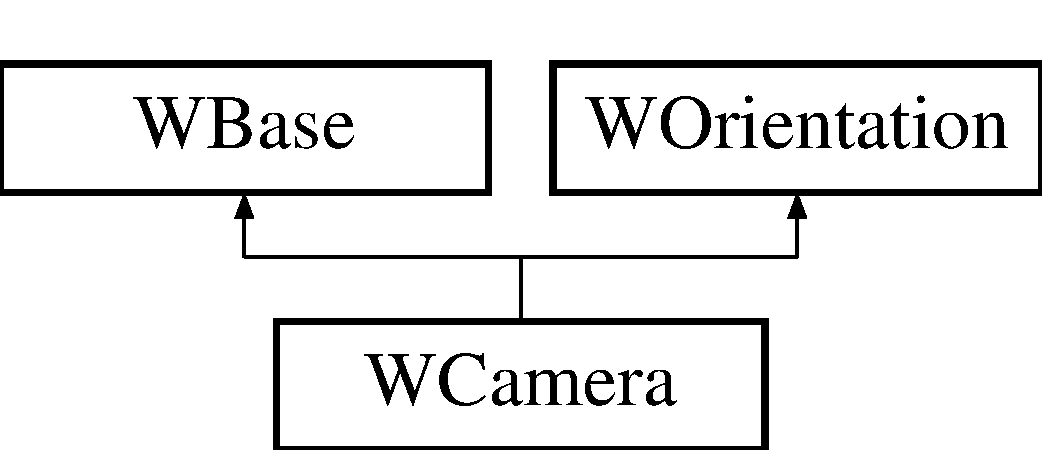
\includegraphics[height=2.000000cm]{class_w_camera}
\end{center}
\end{figure}
\subsection*{Public Member Functions}
\begin{DoxyCompactItemize}
\item 
{\bfseries W\+Camera} (\hyperlink{class_wasabi}{Wasabi} $\ast$const app, unsigned int ID=0)\hypertarget{class_w_camera_a02362e02ece2c149e2abd1f7358f88e7}{}\label{class_w_camera_a02362e02ece2c149e2abd1f7358f88e7}

\item 
void \hyperlink{class_w_camera_a44cd30d5dc870c8a08c200ccca64792f}{On\+State\+Change} (\hyperlink{_w_orientation_8h_afe94de0a48bbd7b343ab18bc318cef28}{S\+T\+A\+T\+E\+\_\+\+C\+H\+A\+N\+G\+E\+\_\+\+T\+Y\+PE} type)
\item 
void \hyperlink{class_w_camera_af59a47532adac71379efd499ec655750}{Update\+Internals} ()
\item 
void \hyperlink{class_w_camera_aa4c4abcba7618888e33984f4220dab03}{Enable\+Auto\+Aspect} ()
\item 
void \hyperlink{class_w_camera_ac8b3661f197c10cf0ffb5dae4ff550ca}{Disable\+Auto\+Aspect} ()
\item 
void \hyperlink{class_w_camera_a18ebb7d402821e7e1e75f807845c842c}{Set\+Range} (float min, float max)
\item 
void \hyperlink{class_w_camera_a846ac55abaf3f25e2dbe1af3aff4ab91}{Set\+F\+OV} (float f\+Value)
\item 
void \hyperlink{class_w_camera_a52ad98e1106f1cc235fca2f303f95cce}{Set\+Aspect} (float aspect)
\item 
void \hyperlink{class_w_camera_a960555526c2bfcd06fc06ba7ac5c5f13}{Set\+Projection\+Type} (\hyperlink{_w_camera_8h_a9a7f9c92f81a74e22c4e4c6f08cd6dde}{W\+\_\+\+P\+R\+O\+J\+E\+C\+T\+I\+O\+N\+T\+Y\+PE} type)
\item 
void \hyperlink{class_w_camera_a90b2aa2474068643e88876ac50639e0e}{Render} (unsigned int width, unsigned int height)
\item 
\hyperlink{class_w_matrix}{W\+Matrix} \hyperlink{class_w_camera_a5a1c340a7bfd239fe3675f27afacfb48}{Get\+View\+Matrix} () const 
\item 
\hyperlink{class_w_matrix}{W\+Matrix} \hyperlink{class_w_camera_a8a579493db789bbc7d2a7c295d161279}{Get\+Projection\+Matrix} (bool b\+Force\+Ortho=false) const 
\item 
float \hyperlink{class_w_camera_af50819dad55bf98e54f3cd046a39d1f8}{Get\+Min\+Range} () const 
\item 
float \hyperlink{class_w_camera_a59ab75c472bbb3af15d1512436d3dc1f}{Get\+Max\+Range} () const 
\item 
float \hyperlink{class_w_camera_a8fabfeba271baa99fdfcae35dd966f1a}{Get\+F\+OV} () const 
\item 
float \hyperlink{class_w_camera_aeb1771e08c8e5f7e5064e0cf66601eb7}{Get\+Aspect} () const 
\item 
bool \hyperlink{class_w_camera_a8cb759213422225c4244f044ed6e0785}{Check\+Point\+In\+Frustum} (float x, float y, float z) const 
\item 
bool \hyperlink{class_w_camera_aebb55c0b8ebf3068b26b552f5f817b57}{Check\+Point\+In\+Frustum} (\hyperlink{class_w_vector3}{W\+Vector3} point) const 
\item 
bool \hyperlink{class_w_camera_a1c8d048c786d1f06fad1d4c626b70c1c}{Check\+Cube\+In\+Frustum} (float x, float y, float z, float radius) const 
\item 
bool \hyperlink{class_w_camera_a67885aed602059895e025348936ffe78}{Check\+Cube\+In\+Frustum} (\hyperlink{class_w_vector3}{W\+Vector3} pos, float radius) const 
\item 
bool \hyperlink{class_w_camera_a40a713c0385c345bb13b69e41c67f89e}{Check\+Sphere\+In\+Frustum} (float x, float y, float z, float radius) const 
\item 
bool \hyperlink{class_w_camera_ad903939a239697caa8f0b7a6dc6fc243}{Check\+Sphere\+In\+Frustum} (\hyperlink{class_w_vector3}{W\+Vector3} pos, float radius) const 
\item 
bool \hyperlink{class_w_camera_a4740f99cef774d046499eb361b5b89a2}{Check\+Box\+In\+Frustum} (float x, float y, float z, float x\+Size, float y\+Size, float z\+Size) const 
\item 
bool \hyperlink{class_w_camera_ade2dbaf0d351b4ae69c88e4fe3cec728}{Check\+Box\+In\+Frustum} (\hyperlink{class_w_vector3}{W\+Vector3} pos, \hyperlink{class_w_vector3}{W\+Vector3} size) const 
\item 
virtual bool \hyperlink{class_w_camera_a21af71c51c191beeec0d1dc5b836cc0c}{Valid} () const 
\end{DoxyCompactItemize}
\subsection*{Additional Inherited Members}


\subsection{Detailed Description}
This implements a camera in \hyperlink{class_wasabi}{Wasabi}. 

\subsection{Member Function Documentation}
\index{W\+Camera@{W\+Camera}!Check\+Box\+In\+Frustum@{Check\+Box\+In\+Frustum}}
\index{Check\+Box\+In\+Frustum@{Check\+Box\+In\+Frustum}!W\+Camera@{W\+Camera}}
\subsubsection[{\texorpdfstring{Check\+Box\+In\+Frustum(float x, float y, float z, float x\+Size, float y\+Size, float z\+Size) const }{CheckBoxInFrustum(float x, float y, float z, float xSize, float ySize, float zSize) const }}]{\setlength{\rightskip}{0pt plus 5cm}bool W\+Camera\+::\+Check\+Box\+In\+Frustum (
\begin{DoxyParamCaption}
\item[{float}]{x, }
\item[{float}]{y, }
\item[{float}]{z, }
\item[{float}]{x\+Size, }
\item[{float}]{y\+Size, }
\item[{float}]{z\+Size}
\end{DoxyParamCaption}
) const}\hypertarget{class_w_camera_a4740f99cef774d046499eb361b5b89a2}{}\label{class_w_camera_a4740f99cef774d046499eb361b5b89a2}
Checks if a given box is in the viewing frustum of the camera 
\begin{DoxyParams}{Parameters}
{\em x} & Box center x \\
\hline
{\em y} & Box center y \\
\hline
{\em z} & Box center z \\
\hline
{\em x\+Size} & Box dimension x from the center to the edge \\
\hline
{\em y\+Size} & Box dimension y from the center to the edge \\
\hline
{\em z\+Size} & Box dimension z from the center to the edge \\
\hline
\end{DoxyParams}
\begin{DoxyReturn}{Returns}
true if the box is in the viewing frustum, false otherwise 
\end{DoxyReturn}
\index{W\+Camera@{W\+Camera}!Check\+Box\+In\+Frustum@{Check\+Box\+In\+Frustum}}
\index{Check\+Box\+In\+Frustum@{Check\+Box\+In\+Frustum}!W\+Camera@{W\+Camera}}
\subsubsection[{\texorpdfstring{Check\+Box\+In\+Frustum(\+W\+Vector3 pos, W\+Vector3 size) const }{CheckBoxInFrustum(WVector3 pos, WVector3 size) const }}]{\setlength{\rightskip}{0pt plus 5cm}bool W\+Camera\+::\+Check\+Box\+In\+Frustum (
\begin{DoxyParamCaption}
\item[{{\bf W\+Vector3}}]{pos, }
\item[{{\bf W\+Vector3}}]{size}
\end{DoxyParamCaption}
) const}\hypertarget{class_w_camera_ade2dbaf0d351b4ae69c88e4fe3cec728}{}\label{class_w_camera_ade2dbaf0d351b4ae69c88e4fe3cec728}
Checks if a given box is in the viewing frustum of the camera 
\begin{DoxyParams}{Parameters}
{\em pos} & Box center \\
\hline
{\em size} & Box dimensions from the center to each edge \\
\hline
\end{DoxyParams}
\begin{DoxyReturn}{Returns}
true if the box is in the viewing frustum, false otherwise 
\end{DoxyReturn}
\index{W\+Camera@{W\+Camera}!Check\+Cube\+In\+Frustum@{Check\+Cube\+In\+Frustum}}
\index{Check\+Cube\+In\+Frustum@{Check\+Cube\+In\+Frustum}!W\+Camera@{W\+Camera}}
\subsubsection[{\texorpdfstring{Check\+Cube\+In\+Frustum(float x, float y, float z, float radius) const }{CheckCubeInFrustum(float x, float y, float z, float radius) const }}]{\setlength{\rightskip}{0pt plus 5cm}bool W\+Camera\+::\+Check\+Cube\+In\+Frustum (
\begin{DoxyParamCaption}
\item[{float}]{x, }
\item[{float}]{y, }
\item[{float}]{z, }
\item[{float}]{radius}
\end{DoxyParamCaption}
) const}\hypertarget{class_w_camera_a1c8d048c786d1f06fad1d4c626b70c1c}{}\label{class_w_camera_a1c8d048c786d1f06fad1d4c626b70c1c}
Checks if a given cube is in the viewing frustum of the camera. 
\begin{DoxyParams}{Parameters}
{\em x} & Cube center x \\
\hline
{\em y} & Cube center y \\
\hline
{\em z} & Cube center z \\
\hline
{\em radius} & Cube diagonal (distance from the center to a corner) \\
\hline
\end{DoxyParams}
\begin{DoxyReturn}{Returns}
true if the cube is in the viewing frustum, false otherwise 
\end{DoxyReturn}
\index{W\+Camera@{W\+Camera}!Check\+Cube\+In\+Frustum@{Check\+Cube\+In\+Frustum}}
\index{Check\+Cube\+In\+Frustum@{Check\+Cube\+In\+Frustum}!W\+Camera@{W\+Camera}}
\subsubsection[{\texorpdfstring{Check\+Cube\+In\+Frustum(\+W\+Vector3 pos, float radius) const }{CheckCubeInFrustum(WVector3 pos, float radius) const }}]{\setlength{\rightskip}{0pt plus 5cm}bool W\+Camera\+::\+Check\+Cube\+In\+Frustum (
\begin{DoxyParamCaption}
\item[{{\bf W\+Vector3}}]{pos, }
\item[{float}]{radius}
\end{DoxyParamCaption}
) const}\hypertarget{class_w_camera_a67885aed602059895e025348936ffe78}{}\label{class_w_camera_a67885aed602059895e025348936ffe78}
Checks if a given cube is in the viewing frustum of the camera. 
\begin{DoxyParams}{Parameters}
{\em pos} & Cube center \\
\hline
{\em radius} & Cube diagonal (distance from the center to a corner) \\
\hline
\end{DoxyParams}
\begin{DoxyReturn}{Returns}
true if the cube is in the viewing frustum, false otherwise 
\end{DoxyReturn}
\index{W\+Camera@{W\+Camera}!Check\+Point\+In\+Frustum@{Check\+Point\+In\+Frustum}}
\index{Check\+Point\+In\+Frustum@{Check\+Point\+In\+Frustum}!W\+Camera@{W\+Camera}}
\subsubsection[{\texorpdfstring{Check\+Point\+In\+Frustum(float x, float y, float z) const }{CheckPointInFrustum(float x, float y, float z) const }}]{\setlength{\rightskip}{0pt plus 5cm}bool W\+Camera\+::\+Check\+Point\+In\+Frustum (
\begin{DoxyParamCaption}
\item[{float}]{x, }
\item[{float}]{y, }
\item[{float}]{z}
\end{DoxyParamCaption}
) const}\hypertarget{class_w_camera_a8cb759213422225c4244f044ed6e0785}{}\label{class_w_camera_a8cb759213422225c4244f044ed6e0785}
Checks if a given point is in the viewing frustum of the camera. 
\begin{DoxyParams}{Parameters}
{\em x} & Point x \\
\hline
{\em y} & Point y \\
\hline
{\em z} & Point z \\
\hline
\end{DoxyParams}
\begin{DoxyReturn}{Returns}
true if (x, y, z) is in the viewing frustum, false otherwise 
\end{DoxyReturn}
\index{W\+Camera@{W\+Camera}!Check\+Point\+In\+Frustum@{Check\+Point\+In\+Frustum}}
\index{Check\+Point\+In\+Frustum@{Check\+Point\+In\+Frustum}!W\+Camera@{W\+Camera}}
\subsubsection[{\texorpdfstring{Check\+Point\+In\+Frustum(\+W\+Vector3 point) const }{CheckPointInFrustum(WVector3 point) const }}]{\setlength{\rightskip}{0pt plus 5cm}bool W\+Camera\+::\+Check\+Point\+In\+Frustum (
\begin{DoxyParamCaption}
\item[{{\bf W\+Vector3}}]{point}
\end{DoxyParamCaption}
) const}\hypertarget{class_w_camera_aebb55c0b8ebf3068b26b552f5f817b57}{}\label{class_w_camera_aebb55c0b8ebf3068b26b552f5f817b57}
Checks if a given point is in the viewing frustum of the camera. 
\begin{DoxyParams}{Parameters}
{\em point} & Point to check \\
\hline
\end{DoxyParams}
\begin{DoxyReturn}{Returns}
true if point is in the viewing frustum, false otherwise 
\end{DoxyReturn}
\index{W\+Camera@{W\+Camera}!Check\+Sphere\+In\+Frustum@{Check\+Sphere\+In\+Frustum}}
\index{Check\+Sphere\+In\+Frustum@{Check\+Sphere\+In\+Frustum}!W\+Camera@{W\+Camera}}
\subsubsection[{\texorpdfstring{Check\+Sphere\+In\+Frustum(float x, float y, float z, float radius) const }{CheckSphereInFrustum(float x, float y, float z, float radius) const }}]{\setlength{\rightskip}{0pt plus 5cm}bool W\+Camera\+::\+Check\+Sphere\+In\+Frustum (
\begin{DoxyParamCaption}
\item[{float}]{x, }
\item[{float}]{y, }
\item[{float}]{z, }
\item[{float}]{radius}
\end{DoxyParamCaption}
) const}\hypertarget{class_w_camera_a40a713c0385c345bb13b69e41c67f89e}{}\label{class_w_camera_a40a713c0385c345bb13b69e41c67f89e}
Checks if a given sphere is in the viewing frustum of the camera. 
\begin{DoxyParams}{Parameters}
{\em x} & Sphere center x \\
\hline
{\em y} & Sphere center y \\
\hline
{\em z} & Sphere center z \\
\hline
{\em radius} & Sphere radius \\
\hline
\end{DoxyParams}
\begin{DoxyReturn}{Returns}
true if the sphere is in the viewing frustum, false otherwise 
\end{DoxyReturn}
\index{W\+Camera@{W\+Camera}!Check\+Sphere\+In\+Frustum@{Check\+Sphere\+In\+Frustum}}
\index{Check\+Sphere\+In\+Frustum@{Check\+Sphere\+In\+Frustum}!W\+Camera@{W\+Camera}}
\subsubsection[{\texorpdfstring{Check\+Sphere\+In\+Frustum(\+W\+Vector3 pos, float radius) const }{CheckSphereInFrustum(WVector3 pos, float radius) const }}]{\setlength{\rightskip}{0pt plus 5cm}bool W\+Camera\+::\+Check\+Sphere\+In\+Frustum (
\begin{DoxyParamCaption}
\item[{{\bf W\+Vector3}}]{pos, }
\item[{float}]{radius}
\end{DoxyParamCaption}
) const}\hypertarget{class_w_camera_ad903939a239697caa8f0b7a6dc6fc243}{}\label{class_w_camera_ad903939a239697caa8f0b7a6dc6fc243}
Checks if a given sphere is in the viewing frustum of the camera. 
\begin{DoxyParams}{Parameters}
{\em pos} & Sphere center \\
\hline
{\em radius} & Sphere radius \\
\hline
\end{DoxyParams}
\begin{DoxyReturn}{Returns}
true if the sphere is in the viewing frustum, false otherwise 
\end{DoxyReturn}
\index{W\+Camera@{W\+Camera}!Disable\+Auto\+Aspect@{Disable\+Auto\+Aspect}}
\index{Disable\+Auto\+Aspect@{Disable\+Auto\+Aspect}!W\+Camera@{W\+Camera}}
\subsubsection[{\texorpdfstring{Disable\+Auto\+Aspect()}{DisableAutoAspect()}}]{\setlength{\rightskip}{0pt plus 5cm}void W\+Camera\+::\+Disable\+Auto\+Aspect (
\begin{DoxyParamCaption}
{}
\end{DoxyParamCaption}
)}\hypertarget{class_w_camera_ac8b3661f197c10cf0ffb5dae4ff550ca}{}\label{class_w_camera_ac8b3661f197c10cf0ffb5dae4ff550ca}
Enables auto aspect ratio calculation when the window/viewport size changes. Auto aspect ratio is calculated as viewport\+\_\+width / viewport\+\_\+height. \index{W\+Camera@{W\+Camera}!Enable\+Auto\+Aspect@{Enable\+Auto\+Aspect}}
\index{Enable\+Auto\+Aspect@{Enable\+Auto\+Aspect}!W\+Camera@{W\+Camera}}
\subsubsection[{\texorpdfstring{Enable\+Auto\+Aspect()}{EnableAutoAspect()}}]{\setlength{\rightskip}{0pt plus 5cm}void W\+Camera\+::\+Enable\+Auto\+Aspect (
\begin{DoxyParamCaption}
{}
\end{DoxyParamCaption}
)}\hypertarget{class_w_camera_aa4c4abcba7618888e33984f4220dab03}{}\label{class_w_camera_aa4c4abcba7618888e33984f4220dab03}
Enables auto aspect ratio calculation when the window/viewport size changes. Auto aspect ratio is calculated as viewport\+\_\+width / viewport\+\_\+height. \index{W\+Camera@{W\+Camera}!Get\+Aspect@{Get\+Aspect}}
\index{Get\+Aspect@{Get\+Aspect}!W\+Camera@{W\+Camera}}
\subsubsection[{\texorpdfstring{Get\+Aspect() const }{GetAspect() const }}]{\setlength{\rightskip}{0pt plus 5cm}float W\+Camera\+::\+Get\+Aspect (
\begin{DoxyParamCaption}
{}
\end{DoxyParamCaption}
) const}\hypertarget{class_w_camera_aeb1771e08c8e5f7e5064e0cf66601eb7}{}\label{class_w_camera_aeb1771e08c8e5f7e5064e0cf66601eb7}
Retrieves the aspect ratio. \begin{DoxyReturn}{Returns}
Aspect ratio 
\end{DoxyReturn}
\index{W\+Camera@{W\+Camera}!Get\+F\+OV@{Get\+F\+OV}}
\index{Get\+F\+OV@{Get\+F\+OV}!W\+Camera@{W\+Camera}}
\subsubsection[{\texorpdfstring{Get\+F\+O\+V() const }{GetFOV() const }}]{\setlength{\rightskip}{0pt plus 5cm}float W\+Camera\+::\+Get\+F\+OV (
\begin{DoxyParamCaption}
{}
\end{DoxyParamCaption}
) const}\hypertarget{class_w_camera_a8fabfeba271baa99fdfcae35dd966f1a}{}\label{class_w_camera_a8fabfeba271baa99fdfcae35dd966f1a}
Retrieves the F\+OV (field of view). \begin{DoxyReturn}{Returns}
F\+OV (field of view) in degrees 
\end{DoxyReturn}
\index{W\+Camera@{W\+Camera}!Get\+Max\+Range@{Get\+Max\+Range}}
\index{Get\+Max\+Range@{Get\+Max\+Range}!W\+Camera@{W\+Camera}}
\subsubsection[{\texorpdfstring{Get\+Max\+Range() const }{GetMaxRange() const }}]{\setlength{\rightskip}{0pt plus 5cm}float W\+Camera\+::\+Get\+Max\+Range (
\begin{DoxyParamCaption}
{}
\end{DoxyParamCaption}
) const}\hypertarget{class_w_camera_a59ab75c472bbb3af15d1512436d3dc1f}{}\label{class_w_camera_a59ab75c472bbb3af15d1512436d3dc1f}
Retrieves the maximum draw distance. \begin{DoxyReturn}{Returns}
Maximum draw distance 
\end{DoxyReturn}
\index{W\+Camera@{W\+Camera}!Get\+Min\+Range@{Get\+Min\+Range}}
\index{Get\+Min\+Range@{Get\+Min\+Range}!W\+Camera@{W\+Camera}}
\subsubsection[{\texorpdfstring{Get\+Min\+Range() const }{GetMinRange() const }}]{\setlength{\rightskip}{0pt plus 5cm}float W\+Camera\+::\+Get\+Min\+Range (
\begin{DoxyParamCaption}
{}
\end{DoxyParamCaption}
) const}\hypertarget{class_w_camera_af50819dad55bf98e54f3cd046a39d1f8}{}\label{class_w_camera_af50819dad55bf98e54f3cd046a39d1f8}
Retrieves the minimum draw distance. \begin{DoxyReturn}{Returns}
Minimum draw distance 
\end{DoxyReturn}
\index{W\+Camera@{W\+Camera}!Get\+Projection\+Matrix@{Get\+Projection\+Matrix}}
\index{Get\+Projection\+Matrix@{Get\+Projection\+Matrix}!W\+Camera@{W\+Camera}}
\subsubsection[{\texorpdfstring{Get\+Projection\+Matrix(bool b\+Force\+Ortho=false) const }{GetProjectionMatrix(bool bForceOrtho=false) const }}]{\setlength{\rightskip}{0pt plus 5cm}{\bf W\+Matrix} W\+Camera\+::\+Get\+Projection\+Matrix (
\begin{DoxyParamCaption}
\item[{bool}]{b\+Force\+Ortho = {\ttfamily false}}
\end{DoxyParamCaption}
) const}\hypertarget{class_w_camera_a8a579493db789bbc7d2a7c295d161279}{}\label{class_w_camera_a8a579493db789bbc7d2a7c295d161279}
Retrieves the current projection matrix \begin{DoxyReturn}{Returns}
Current projection matrix Retrieves the current projection matrix 
\end{DoxyReturn}

\begin{DoxyParams}{Parameters}
{\em b\+Force\+Ortho} & If set to true, the returned projection matrix will be forcefully set to use P\+R\+O\+J\+E\+C\+T\+I\+O\+N\+\_\+\+O\+R\+T\+H\+O\+G\+O\+N\+AL for this call \\
\hline
\end{DoxyParams}
\begin{DoxyReturn}{Returns}
Current projection matrix 
\end{DoxyReturn}
\index{W\+Camera@{W\+Camera}!Get\+View\+Matrix@{Get\+View\+Matrix}}
\index{Get\+View\+Matrix@{Get\+View\+Matrix}!W\+Camera@{W\+Camera}}
\subsubsection[{\texorpdfstring{Get\+View\+Matrix() const }{GetViewMatrix() const }}]{\setlength{\rightskip}{0pt plus 5cm}{\bf W\+Matrix} W\+Camera\+::\+Get\+View\+Matrix (
\begin{DoxyParamCaption}
{}
\end{DoxyParamCaption}
) const}\hypertarget{class_w_camera_a5a1c340a7bfd239fe3675f27afacfb48}{}\label{class_w_camera_a5a1c340a7bfd239fe3675f27afacfb48}
Retrieves the current view matrix \begin{DoxyReturn}{Returns}
Current view matrix 
\end{DoxyReturn}
\index{W\+Camera@{W\+Camera}!On\+State\+Change@{On\+State\+Change}}
\index{On\+State\+Change@{On\+State\+Change}!W\+Camera@{W\+Camera}}
\subsubsection[{\texorpdfstring{On\+State\+Change(\+S\+T\+A\+T\+E\+\_\+\+C\+H\+A\+N\+G\+E\+\_\+\+T\+Y\+P\+E type)}{OnStateChange(STATE_CHANGE_TYPE type)}}]{\setlength{\rightskip}{0pt plus 5cm}void W\+Camera\+::\+On\+State\+Change (
\begin{DoxyParamCaption}
\item[{{\bf S\+T\+A\+T\+E\+\_\+\+C\+H\+A\+N\+G\+E\+\_\+\+T\+Y\+PE}}]{type}
\end{DoxyParamCaption}
)\hspace{0.3cm}{\ttfamily [virtual]}}\hypertarget{class_w_camera_a44cd30d5dc870c8a08c200ccca64792f}{}\label{class_w_camera_a44cd30d5dc870c8a08c200ccca64792f}
This is a callback (inherited from \hyperlink{class_w_orientation}{W\+Orientation}) to inform this object of a change in orientation. 
\begin{DoxyParams}{Parameters}
{\em type} & Orientation change type (rotation or motion) \\
\hline
\end{DoxyParams}


Reimplemented from \hyperlink{class_w_orientation_aa765b7dcd772bbcc511c2c9317e7693c}{W\+Orientation}.

\index{W\+Camera@{W\+Camera}!Render@{Render}}
\index{Render@{Render}!W\+Camera@{W\+Camera}}
\subsubsection[{\texorpdfstring{Render(unsigned int width, unsigned int height)}{Render(unsigned int width, unsigned int height)}}]{\setlength{\rightskip}{0pt plus 5cm}void W\+Camera\+::\+Render (
\begin{DoxyParamCaption}
\item[{unsigned int}]{width, }
\item[{unsigned int}]{height}
\end{DoxyParamCaption}
)}\hypertarget{class_w_camera_a90b2aa2474068643e88876ac50639e0e}{}\label{class_w_camera_a90b2aa2474068643e88876ac50639e0e}
Prepares the camera such that its\textquotesingle{} matrices can be used to perform transformations such as object rendering. 
\begin{DoxyParams}{Parameters}
{\em width} & Width of the rendering viewport \\
\hline
{\em height} & Height of the rendering viewport \\
\hline
\end{DoxyParams}
\index{W\+Camera@{W\+Camera}!Set\+Aspect@{Set\+Aspect}}
\index{Set\+Aspect@{Set\+Aspect}!W\+Camera@{W\+Camera}}
\subsubsection[{\texorpdfstring{Set\+Aspect(float aspect)}{SetAspect(float aspect)}}]{\setlength{\rightskip}{0pt plus 5cm}void W\+Camera\+::\+Set\+Aspect (
\begin{DoxyParamCaption}
\item[{float}]{aspect}
\end{DoxyParamCaption}
)}\hypertarget{class_w_camera_a52ad98e1106f1cc235fca2f303f95cce}{}\label{class_w_camera_a52ad98e1106f1cc235fca2f303f95cce}
Sets the aspect ratio. If auto aspect ratio is enabled, this will be overridden on the next \hyperlink{class_w_camera_af59a47532adac71379efd499ec655750}{Update\+Internals()} or \hyperlink{class_w_camera_a90b2aa2474068643e88876ac50639e0e}{Render()}. 
\begin{DoxyParams}{Parameters}
{\em aspect} & New aspect ratio \\
\hline
\end{DoxyParams}
\index{W\+Camera@{W\+Camera}!Set\+F\+OV@{Set\+F\+OV}}
\index{Set\+F\+OV@{Set\+F\+OV}!W\+Camera@{W\+Camera}}
\subsubsection[{\texorpdfstring{Set\+F\+O\+V(float f\+Value)}{SetFOV(float fValue)}}]{\setlength{\rightskip}{0pt plus 5cm}void W\+Camera\+::\+Set\+F\+OV (
\begin{DoxyParamCaption}
\item[{float}]{f\+Value}
\end{DoxyParamCaption}
)}\hypertarget{class_w_camera_a846ac55abaf3f25e2dbe1af3aff4ab91}{}\label{class_w_camera_a846ac55abaf3f25e2dbe1af3aff4ab91}
Set the F\+OV (field of view) for the camera. 
\begin{DoxyParams}{Parameters}
{\em f\+Value} & New field of view, in degrees \\
\hline
\end{DoxyParams}
\index{W\+Camera@{W\+Camera}!Set\+Projection\+Type@{Set\+Projection\+Type}}
\index{Set\+Projection\+Type@{Set\+Projection\+Type}!W\+Camera@{W\+Camera}}
\subsubsection[{\texorpdfstring{Set\+Projection\+Type(\+W\+\_\+\+P\+R\+O\+J\+E\+C\+T\+I\+O\+N\+T\+Y\+P\+E type)}{SetProjectionType(W_PROJECTIONTYPE type)}}]{\setlength{\rightskip}{0pt plus 5cm}void W\+Camera\+::\+Set\+Projection\+Type (
\begin{DoxyParamCaption}
\item[{{\bf W\+\_\+\+P\+R\+O\+J\+E\+C\+T\+I\+O\+N\+T\+Y\+PE}}]{type}
\end{DoxyParamCaption}
)}\hypertarget{class_w_camera_a960555526c2bfcd06fc06ba7ac5c5f13}{}\label{class_w_camera_a960555526c2bfcd06fc06ba7ac5c5f13}
Sets the projection type for this camera. 
\begin{DoxyParams}{Parameters}
{\em type} & Type of projection \\
\hline
\end{DoxyParams}
\index{W\+Camera@{W\+Camera}!Set\+Range@{Set\+Range}}
\index{Set\+Range@{Set\+Range}!W\+Camera@{W\+Camera}}
\subsubsection[{\texorpdfstring{Set\+Range(float min, float max)}{SetRange(float min, float max)}}]{\setlength{\rightskip}{0pt plus 5cm}void W\+Camera\+::\+Set\+Range (
\begin{DoxyParamCaption}
\item[{float}]{min, }
\item[{float}]{max}
\end{DoxyParamCaption}
)}\hypertarget{class_w_camera_a18ebb7d402821e7e1e75f807845c842c}{}\label{class_w_camera_a18ebb7d402821e7e1e75f807845c842c}
Sets the range in which the camera can see. The camera cannot render closer to it than min and farther to it than max. 
\begin{DoxyParams}{Parameters}
{\em min} & minimum draw distance \\
\hline
{\em max} & maximum draw distance \\
\hline
\end{DoxyParams}
\index{W\+Camera@{W\+Camera}!Update\+Internals@{Update\+Internals}}
\index{Update\+Internals@{Update\+Internals}!W\+Camera@{W\+Camera}}
\subsubsection[{\texorpdfstring{Update\+Internals()}{UpdateInternals()}}]{\setlength{\rightskip}{0pt plus 5cm}void W\+Camera\+::\+Update\+Internals (
\begin{DoxyParamCaption}
{}
\end{DoxyParamCaption}
)}\hypertarget{class_w_camera_af59a47532adac71379efd499ec655750}{}\label{class_w_camera_af59a47532adac71379efd499ec655750}
Update the matrices to match the latest changes. This is automatically called during rendering of a camera. \index{W\+Camera@{W\+Camera}!Valid@{Valid}}
\index{Valid@{Valid}!W\+Camera@{W\+Camera}}
\subsubsection[{\texorpdfstring{Valid() const }{Valid() const }}]{\setlength{\rightskip}{0pt plus 5cm}bool W\+Camera\+::\+Valid (
\begin{DoxyParamCaption}
\item[{void}]{}
\end{DoxyParamCaption}
) const\hspace{0.3cm}{\ttfamily [virtual]}}\hypertarget{class_w_camera_a21af71c51c191beeec0d1dc5b836cc0c}{}\label{class_w_camera_a21af71c51c191beeec0d1dc5b836cc0c}
Checks if the camera is valid (always true). \begin{DoxyReturn}{Returns}
true 
\end{DoxyReturn}


Implements \hyperlink{class_w_base_a76ac973ba9a43e182f6a6a4869d69725}{W\+Base}.



The documentation for this class was generated from the following files\+:\begin{DoxyCompactItemize}
\item 
Wasabi/\+Cameras/\hyperlink{_w_camera_8h}{W\+Camera.\+h}\item 
Wasabi/\+Cameras/W\+Camera.\+cpp\end{DoxyCompactItemize}

\hypertarget{class_w_camera_manager}{}\section{W\+Camera\+Manager Class Reference}
\label{class_w_camera_manager}\index{W\+Camera\+Manager@{W\+Camera\+Manager}}


{\ttfamily \#include $<$W\+Camera.\+h$>$}

Inheritance diagram for W\+Camera\+Manager\+:\begin{figure}[H]
\begin{center}
\leavevmode
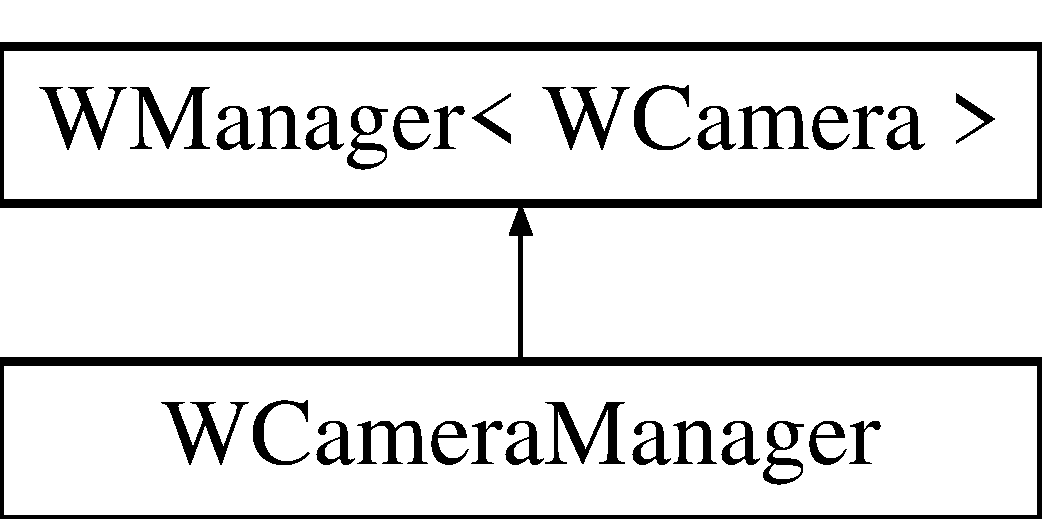
\includegraphics[height=2.000000cm]{class_w_camera_manager}
\end{center}
\end{figure}
\subsection*{Public Member Functions}
\begin{DoxyCompactItemize}
\item 
{\bfseries W\+Camera\+Manager} (\hyperlink{class_wasabi}{Wasabi} $\ast$const app)\hypertarget{class_w_camera_manager_aee9651ebfbf1e66456b10b191cc1dbf5}{}\label{class_w_camera_manager_aee9651ebfbf1e66456b10b191cc1dbf5}

\item 
\hyperlink{class_w_error}{W\+Error} \hyperlink{class_w_camera_manager_a40f417e67c5d51ba5a5a00ce284f63c2}{Load} ()
\item 
\hyperlink{class_w_camera}{W\+Camera} $\ast$ \hyperlink{class_w_camera_manager_a4b691395b3febca183af76eafc88808b}{Get\+Default\+Camera} () const 
\end{DoxyCompactItemize}
\subsection*{Additional Inherited Members}


\subsection{Detailed Description}
Manager class for \hyperlink{class_w_camera}{W\+Camera}. 

\subsection{Member Function Documentation}
\index{W\+Camera\+Manager@{W\+Camera\+Manager}!Get\+Default\+Camera@{Get\+Default\+Camera}}
\index{Get\+Default\+Camera@{Get\+Default\+Camera}!W\+Camera\+Manager@{W\+Camera\+Manager}}
\subsubsection[{\texorpdfstring{Get\+Default\+Camera() const }{GetDefaultCamera() const }}]{\setlength{\rightskip}{0pt plus 5cm}{\bf W\+Camera} $\ast$ W\+Camera\+Manager\+::\+Get\+Default\+Camera (
\begin{DoxyParamCaption}
{}
\end{DoxyParamCaption}
) const}\hypertarget{class_w_camera_manager_a4b691395b3febca183af76eafc88808b}{}\label{class_w_camera_manager_a4b691395b3febca183af76eafc88808b}
Retrieves a pointer to the default camera. \begin{DoxyReturn}{Returns}
Pointer to the default camera 
\end{DoxyReturn}
\index{W\+Camera\+Manager@{W\+Camera\+Manager}!Load@{Load}}
\index{Load@{Load}!W\+Camera\+Manager@{W\+Camera\+Manager}}
\subsubsection[{\texorpdfstring{Load()}{Load()}}]{\setlength{\rightskip}{0pt plus 5cm}{\bf W\+Error} W\+Camera\+Manager\+::\+Load (
\begin{DoxyParamCaption}
{}
\end{DoxyParamCaption}
)}\hypertarget{class_w_camera_manager_a40f417e67c5d51ba5a5a00ce284f63c2}{}\label{class_w_camera_manager_a40f417e67c5d51ba5a5a00ce284f63c2}
Prepare the Camera manager and create the default camera. \begin{DoxyReturn}{Returns}
Error code, see \hyperlink{_w_error_8h}{W\+Error.\+h} 
\end{DoxyReturn}


The documentation for this class was generated from the following files\+:\begin{DoxyCompactItemize}
\item 
Wasabi/\+Cameras/\hyperlink{_w_camera_8h}{W\+Camera.\+h}\item 
Wasabi/\+Cameras/W\+Camera.\+cpp\end{DoxyCompactItemize}

\hypertarget{class_w_color}{}\section{W\+Color Class Reference}
\label{class_w_color}\index{W\+Color@{W\+Color}}


{\ttfamily \#include $<$W\+Math.\+h$>$}

\subsection*{Public Member Functions}
\begin{DoxyCompactItemize}
\item 
{\bfseries W\+Color} (float f\+R\+GB)\hypertarget{class_w_color_a5dc0ff89bb900ca42dd8451152296932}{}\label{class_w_color_a5dc0ff89bb900ca42dd8451152296932}

\item 
{\bfseries W\+Color} (float fR, float fG, float fB)\hypertarget{class_w_color_a27b443eb5f19c2c58fb32bfe55503770}{}\label{class_w_color_a27b443eb5f19c2c58fb32bfe55503770}

\item 
{\bfseries W\+Color} (float fR, float fG, float fB, float fA)\hypertarget{class_w_color_a16123034ea200d0c251e10e900e612cf}{}\label{class_w_color_a16123034ea200d0c251e10e900e612cf}

\item 
{\bfseries operator float $\ast$} ()\hypertarget{class_w_color_a0b06e9dfce8e662baa203552d341145c}{}\label{class_w_color_a0b06e9dfce8e662baa203552d341145c}

\item 
{\bfseries operator const float $\ast$} ()\hypertarget{class_w_color_ab0953e49390ec00766c60733713d0de4}{}\label{class_w_color_ab0953e49390ec00766c60733713d0de4}

\item 
const \hyperlink{class_w_color}{W\+Color} {\bfseries operator+} () const \hypertarget{class_w_color_a0a12901a5c1aaf8989648d616aa555c3}{}\label{class_w_color_a0a12901a5c1aaf8989648d616aa555c3}

\item 
const \hyperlink{class_w_color}{W\+Color} {\bfseries operator-\/} () const \hypertarget{class_w_color_a7b1e53c97d5c7974a07eeef59fbb458c}{}\label{class_w_color_a7b1e53c97d5c7974a07eeef59fbb458c}

\item 
const \hyperlink{class_w_color}{W\+Color} {\bfseries operator+} (const \hyperlink{class_w_color}{W\+Color} col) const \hypertarget{class_w_color_adaa18f12f3a7316beded3e040c936d96}{}\label{class_w_color_adaa18f12f3a7316beded3e040c936d96}

\item 
const \hyperlink{class_w_color}{W\+Color} {\bfseries operator-\/} (const \hyperlink{class_w_color}{W\+Color} col) const \hypertarget{class_w_color_a34ff188b2bf3a82cc5ea8978756ec207}{}\label{class_w_color_a34ff188b2bf3a82cc5ea8978756ec207}

\item 
const \hyperlink{class_w_color}{W\+Color} {\bfseries operator$\ast$} (const \hyperlink{class_w_color}{W\+Color} col) const \hypertarget{class_w_color_a693d15a5e4d09deefc8ef39a743cb3d0}{}\label{class_w_color_a693d15a5e4d09deefc8ef39a743cb3d0}

\item 
const \hyperlink{class_w_color}{W\+Color} {\bfseries operator$\ast$} (const float f) const \hypertarget{class_w_color_a5b61354d4d937c469a562d5492b0db12}{}\label{class_w_color_a5b61354d4d937c469a562d5492b0db12}

\item 
const \hyperlink{class_w_color}{W\+Color} {\bfseries operator/} (const \hyperlink{class_w_color}{W\+Color} col) const \hypertarget{class_w_color_a0c08f33a826df055d2e84057c887ec16}{}\label{class_w_color_a0c08f33a826df055d2e84057c887ec16}

\item 
const \hyperlink{class_w_color}{W\+Color} {\bfseries operator/} (const float f) const \hypertarget{class_w_color_ad7b46b7048d4aea9c3d195ab3833eb8a}{}\label{class_w_color_ad7b46b7048d4aea9c3d195ab3833eb8a}

\item 
void {\bfseries operator+=} (const \hyperlink{class_w_color}{W\+Color} col)\hypertarget{class_w_color_a26a45fa3192e93dfba4ea7f8f62f42a2}{}\label{class_w_color_a26a45fa3192e93dfba4ea7f8f62f42a2}

\item 
void {\bfseries operator-\/=} (const \hyperlink{class_w_color}{W\+Color} col)\hypertarget{class_w_color_a3d2337783b0a2ff94f19c51d45f6b729}{}\label{class_w_color_a3d2337783b0a2ff94f19c51d45f6b729}

\item 
void {\bfseries operator$\ast$=} (const \hyperlink{class_w_color}{W\+Color} col)\hypertarget{class_w_color_a02a2bd936d7589d6462440c901f7df28}{}\label{class_w_color_a02a2bd936d7589d6462440c901f7df28}

\item 
void {\bfseries operator$\ast$=} (const float f)\hypertarget{class_w_color_a6292148e15f11fa942542102a02cf035}{}\label{class_w_color_a6292148e15f11fa942542102a02cf035}

\item 
void {\bfseries operator/=} (const \hyperlink{class_w_color}{W\+Color} col)\hypertarget{class_w_color_add8d77caf11f1c0e8235b3fa74692efc}{}\label{class_w_color_add8d77caf11f1c0e8235b3fa74692efc}

\item 
void {\bfseries operator/=} (const float f)\hypertarget{class_w_color_a6b0b3acf6841764fb82384567b96dd8e}{}\label{class_w_color_a6b0b3acf6841764fb82384567b96dd8e}

\item 
float \& {\bfseries operator\mbox{[}$\,$\mbox{]}} (const unsigned int index)\hypertarget{class_w_color_a5ae7ed83d4a85c202c8eb4720d14c5f7}{}\label{class_w_color_a5ae7ed83d4a85c202c8eb4720d14c5f7}

\item 
const float {\bfseries operator\mbox{[}$\,$\mbox{]}} (const unsigned int index) const \hypertarget{class_w_color_ab91a9be2af138122e31898cb98a2e91c}{}\label{class_w_color_ab91a9be2af138122e31898cb98a2e91c}

\item 
float \& {\bfseries operator\mbox{[}$\,$\mbox{]}} (const int index)\hypertarget{class_w_color_a718fd12567cccd948deacf892c446f84}{}\label{class_w_color_a718fd12567cccd948deacf892c446f84}

\item 
const float {\bfseries operator\mbox{[}$\,$\mbox{]}} (const int index) const \hypertarget{class_w_color_af83a4694ef5d421f04a1ef165b1c7979}{}\label{class_w_color_af83a4694ef5d421f04a1ef165b1c7979}

\item 
float \& {\bfseries operator()} (const unsigned int index)\hypertarget{class_w_color_ae1e3db9bfe624a8bc1e804c6b5767ab2}{}\label{class_w_color_ae1e3db9bfe624a8bc1e804c6b5767ab2}

\item 
const float {\bfseries operator()} (const unsigned int index) const \hypertarget{class_w_color_a75bae865ab87d24275b849fdde6479e5}{}\label{class_w_color_a75bae865ab87d24275b849fdde6479e5}

\item 
float \& {\bfseries operator()} (const int index)\hypertarget{class_w_color_a352fc62cb9f7654b94ed839112cc44f5}{}\label{class_w_color_a352fc62cb9f7654b94ed839112cc44f5}

\item 
const float {\bfseries operator()} (const int index) const \hypertarget{class_w_color_ae5893f27647e8d498ef75c4c8af01f73}{}\label{class_w_color_ae5893f27647e8d498ef75c4c8af01f73}

\item 
const bool {\bfseries operator==} (const \hyperlink{class_w_color}{W\+Color} col) const \hypertarget{class_w_color_abe6cb73e17d5cdcd032e750c9e0d7251}{}\label{class_w_color_abe6cb73e17d5cdcd032e750c9e0d7251}

\item 
const bool {\bfseries operator!=} (const \hyperlink{class_w_color}{W\+Color} col) const \hypertarget{class_w_color_aa7aa6dbf409555002a28b1ab6d05ef75}{}\label{class_w_color_aa7aa6dbf409555002a28b1ab6d05ef75}

\end{DoxyCompactItemize}
\subsection*{Public Attributes}
\begin{DoxyCompactItemize}
\item 
float \hyperlink{class_w_color_a0bdf6acf580fb1607bed90cb01596444}{r}
\item 
float \hyperlink{class_w_color_aea6616f49cdb611d9a519787a692ce31}{g}
\item 
float \hyperlink{class_w_color_a740e9174ff78cba98a391f6e5b319192}{b}
\item 
float \hyperlink{class_w_color_add453fb03a2f570d04d20458f166b9e0}{a}
\end{DoxyCompactItemize}
\subsection*{Friends}
\begin{DoxyCompactItemize}
\item 
const \hyperlink{class_w_color}{W\+Color} {\bfseries operator$\ast$} (const float f, const \hyperlink{class_w_color}{W\+Color} v)\hypertarget{class_w_color_ac5d19f22943f6c287df4d420dd06cbc5}{}\label{class_w_color_ac5d19f22943f6c287df4d420dd06cbc5}

\item 
const \hyperlink{class_w_color}{W\+Color} {\bfseries operator/} (const float f, const \hyperlink{class_w_color}{W\+Color} v)\hypertarget{class_w_color_a791afa90ccd5a4b4ca8dae450c0478ac}{}\label{class_w_color_a791afa90ccd5a4b4ca8dae450c0478ac}

\end{DoxyCompactItemize}


\subsection{Detailed Description}
Represents a color. 

\subsection{Member Data Documentation}
\index{W\+Color@{W\+Color}!a@{a}}
\index{a@{a}!W\+Color@{W\+Color}}
\subsubsection[{\texorpdfstring{a}{a}}]{\setlength{\rightskip}{0pt plus 5cm}float W\+Color\+::a}\hypertarget{class_w_color_add453fb03a2f570d04d20458f166b9e0}{}\label{class_w_color_add453fb03a2f570d04d20458f166b9e0}
alpha component of the color \index{W\+Color@{W\+Color}!b@{b}}
\index{b@{b}!W\+Color@{W\+Color}}
\subsubsection[{\texorpdfstring{b}{b}}]{\setlength{\rightskip}{0pt plus 5cm}float W\+Color\+::b}\hypertarget{class_w_color_a740e9174ff78cba98a391f6e5b319192}{}\label{class_w_color_a740e9174ff78cba98a391f6e5b319192}
blue component of the color \index{W\+Color@{W\+Color}!g@{g}}
\index{g@{g}!W\+Color@{W\+Color}}
\subsubsection[{\texorpdfstring{g}{g}}]{\setlength{\rightskip}{0pt plus 5cm}float W\+Color\+::g}\hypertarget{class_w_color_aea6616f49cdb611d9a519787a692ce31}{}\label{class_w_color_aea6616f49cdb611d9a519787a692ce31}
green component of the color \index{W\+Color@{W\+Color}!r@{r}}
\index{r@{r}!W\+Color@{W\+Color}}
\subsubsection[{\texorpdfstring{r}{r}}]{\setlength{\rightskip}{0pt plus 5cm}float W\+Color\+::r}\hypertarget{class_w_color_a0bdf6acf580fb1607bed90cb01596444}{}\label{class_w_color_a0bdf6acf580fb1607bed90cb01596444}
red component of the color 

The documentation for this class was generated from the following file\+:\begin{DoxyCompactItemize}
\item 
Wasabi/\+Core/W\+Math.\+h\end{DoxyCompactItemize}

\hypertarget{class_w_constraint}{}\section{W\+Constraint Class Reference}
\label{class_w_constraint}\index{W\+Constraint@{W\+Constraint}}
Inheritance diagram for W\+Constraint\+:\begin{figure}[H]
\begin{center}
\leavevmode
\includegraphics[height=2.014389cm]{class_w_constraint}
\end{center}
\end{figure}
\subsection*{Public Member Functions}
\begin{DoxyCompactItemize}
\item 
{\bfseries W\+Constraint} (class \hyperlink{class_wasabi}{Wasabi} $\ast$const app, unsigned int ID=0)\hypertarget{class_w_constraint_a21b990edbd3f3dc64e922ffb821e7d14}{}\label{class_w_constraint_a21b990edbd3f3dc64e922ffb821e7d14}

\item 
virtual void {\bfseries Build} (const \hyperlink{class_w_rigid_body}{W\+Rigid\+Body} $\ast$const rb1, const \hyperlink{class_w_rigid_body}{W\+Rigid\+Body} $\ast$const rb2, bool breakable=false)=0\hypertarget{class_w_constraint_a9bb986fc73ef934d3d79055b1f124047}{}\label{class_w_constraint_a9bb986fc73ef934d3d79055b1f124047}

\item 
void {\bfseries Set\+Breaking\+Threshold} (float threshold)\hypertarget{class_w_constraint_a8faa2422e6e1b740c8f8aa3cd44d00b0}{}\label{class_w_constraint_a8faa2422e6e1b740c8f8aa3cd44d00b0}

\item 
void {\bfseries Set\+Max\+Linear\+Impulse} (float impulse)\hypertarget{class_w_constraint_a5e5b025ad26fe59ebe3fba98712f120e}{}\label{class_w_constraint_a5e5b025ad26fe59ebe3fba98712f120e}

\item 
hkp\+Constraint\+Data $\ast$ {\bfseries Get\+Constraint} () const \hypertarget{class_w_constraint_ab1d212004a66467136f3358430b612eb}{}\label{class_w_constraint_ab1d212004a66467136f3358430b612eb}

\item 
bool \hyperlink{class_w_constraint_aea99eb105fd8eca22f40bc67b5214590}{Valid} () const 
\end{DoxyCompactItemize}
\subsection*{Protected Attributes}
\begin{DoxyCompactItemize}
\item 
hkp\+Rigid\+Body $\ast$ {\bfseries m\+\_\+rb1}\hypertarget{class_w_constraint_a16b25d8b2b15de94113bef9d4eb68c26}{}\label{class_w_constraint_a16b25d8b2b15de94113bef9d4eb68c26}

\item 
hkp\+Rigid\+Body $\ast$ {\bfseries m\+\_\+rb2}\hypertarget{class_w_constraint_a116417885767b190e89c4df25b083c0a}{}\label{class_w_constraint_a116417885767b190e89c4df25b083c0a}

\item 
hkp\+World $\ast$ {\bfseries m\+\_\+world}\hypertarget{class_w_constraint_ad9333fa6af638f4a932e29d19316e06c}{}\label{class_w_constraint_ad9333fa6af638f4a932e29d19316e06c}

\item 
hkp\+Constraint\+Data $\ast$ {\bfseries m\+\_\+constraint}\hypertarget{class_w_constraint_a60718e4ef138d3b2c51abe73e2f259d9}{}\label{class_w_constraint_a60718e4ef138d3b2c51abe73e2f259d9}

\item 
hkp\+Constraint\+Instance $\ast$ {\bfseries m\+\_\+instance}\hypertarget{class_w_constraint_ab3f36126a2bbe8cb04afe4e2b1c9e998}{}\label{class_w_constraint_ab3f36126a2bbe8cb04afe4e2b1c9e998}

\item 
hkp\+Breakable\+Constraint\+Data $\ast$ {\bfseries m\+\_\+breakable\+Constraint}\hypertarget{class_w_constraint_a97a3c191939cb484aeef4d65f91aaee3}{}\label{class_w_constraint_a97a3c191939cb484aeef4d65f91aaee3}

\end{DoxyCompactItemize}


\subsection{Member Function Documentation}
\index{W\+Constraint@{W\+Constraint}!Valid@{Valid}}
\index{Valid@{Valid}!W\+Constraint@{W\+Constraint}}
\subsubsection[{\texorpdfstring{Valid() const }{Valid() const }}]{\setlength{\rightskip}{0pt plus 5cm}bool W\+Constraint\+::\+Valid (
\begin{DoxyParamCaption}
{}
\end{DoxyParamCaption}
) const\hspace{0.3cm}{\ttfamily [virtual]}}\hypertarget{class_w_constraint_aea99eb105fd8eca22f40bc67b5214590}{}\label{class_w_constraint_aea99eb105fd8eca22f40bc67b5214590}
Must be implemented by the child. This function should report the validity status of the object, in whatever sense of \char`\"{}validity\char`\"{} it chooses. \begin{DoxyReturn}{Returns}
true if the object is \char`\"{}valid\char`\"{}, false otherwise 
\end{DoxyReturn}


Implements \hyperlink{class_w_base_a76ac973ba9a43e182f6a6a4869d69725}{W\+Base}.



The documentation for this class was generated from the following file\+:\begin{DoxyCompactItemize}
\item 
Wasabi/\+Physics/\+Havok/W\+Havok\+Physics.\+h\end{DoxyCompactItemize}

\hypertarget{class_w_constraint_manager}{}\section{W\+Constraint\+Manager Class Reference}
\label{class_w_constraint_manager}\index{W\+Constraint\+Manager@{W\+Constraint\+Manager}}
Inheritance diagram for W\+Constraint\+Manager\+:\begin{figure}[H]
\begin{center}
\leavevmode
\includegraphics[height=2.000000cm]{class_w_constraint_manager}
\end{center}
\end{figure}
\subsection*{Public Member Functions}
\begin{DoxyCompactItemize}
\item 
{\bfseries W\+Constraint\+Manager} (\hyperlink{class_wasabi}{Wasabi} $\ast$const app)\hypertarget{class_w_constraint_manager_a506ce1985f9d98a530f7ad7c42f8e59f}{}\label{class_w_constraint_manager_a506ce1985f9d98a530f7ad7c42f8e59f}

\end{DoxyCompactItemize}
\subsection*{Additional Inherited Members}


The documentation for this class was generated from the following file\+:\begin{DoxyCompactItemize}
\item 
Wasabi/\+Physics/\+Havok/W\+Havok\+Physics.\+h\end{DoxyCompactItemize}

\hypertarget{struct_w_default_vertex}{}\section{W\+Default\+Vertex Struct Reference}
\label{struct_w_default_vertex}\index{W\+Default\+Vertex@{W\+Default\+Vertex}}


{\ttfamily \#include $<$W\+Geometry.\+h$>$}

\subsection*{Public Member Functions}
\begin{DoxyCompactItemize}
\item 
{\bfseries W\+Default\+Vertex} (float x, float y, float z, float tx, float ty, float tz, float nx, float ny, float nz, float u, float v)\hypertarget{struct_w_default_vertex_a119df88c3ef93fd08ce657af30c08669}{}\label{struct_w_default_vertex_a119df88c3ef93fd08ce657af30c08669}

\end{DoxyCompactItemize}
\subsection*{Public Attributes}
\begin{DoxyCompactItemize}
\item 
\hyperlink{class_w_vector3}{W\+Vector3} \hyperlink{struct_w_default_vertex_afdcf7f42cc5581df2f6952aaf839e8bb}{pos}
\item 
\hyperlink{class_w_vector3}{W\+Vector3} \hyperlink{struct_w_default_vertex_a2220549f6c898e6fdc5f534630c44796}{tang}
\item 
\hyperlink{class_w_vector3}{W\+Vector3} \hyperlink{struct_w_default_vertex_a60a322ede7963e1e4a3f6e031c303ffa}{norm}
\item 
\hyperlink{class_w_vector2}{W\+Vector2} \hyperlink{struct_w_default_vertex_a3e58deb0c88b8adaa8423aebd8427172}{texC}
\end{DoxyCompactItemize}


\subsection{Detailed Description}
This represents the default vertex structure used by the engine. 

\subsection{Member Data Documentation}
\index{W\+Default\+Vertex@{W\+Default\+Vertex}!norm@{norm}}
\index{norm@{norm}!W\+Default\+Vertex@{W\+Default\+Vertex}}
\subsubsection[{\texorpdfstring{norm}{norm}}]{\setlength{\rightskip}{0pt plus 5cm}{\bf W\+Vector3} W\+Default\+Vertex\+::norm}\hypertarget{struct_w_default_vertex_a60a322ede7963e1e4a3f6e031c303ffa}{}\label{struct_w_default_vertex_a60a322ede7963e1e4a3f6e031c303ffa}
Normal attribute \index{W\+Default\+Vertex@{W\+Default\+Vertex}!pos@{pos}}
\index{pos@{pos}!W\+Default\+Vertex@{W\+Default\+Vertex}}
\subsubsection[{\texorpdfstring{pos}{pos}}]{\setlength{\rightskip}{0pt plus 5cm}{\bf W\+Vector3} W\+Default\+Vertex\+::pos}\hypertarget{struct_w_default_vertex_afdcf7f42cc5581df2f6952aaf839e8bb}{}\label{struct_w_default_vertex_afdcf7f42cc5581df2f6952aaf839e8bb}
Position attribute \index{W\+Default\+Vertex@{W\+Default\+Vertex}!tang@{tang}}
\index{tang@{tang}!W\+Default\+Vertex@{W\+Default\+Vertex}}
\subsubsection[{\texorpdfstring{tang}{tang}}]{\setlength{\rightskip}{0pt plus 5cm}{\bf W\+Vector3} W\+Default\+Vertex\+::tang}\hypertarget{struct_w_default_vertex_a2220549f6c898e6fdc5f534630c44796}{}\label{struct_w_default_vertex_a2220549f6c898e6fdc5f534630c44796}
Tangent attribute \index{W\+Default\+Vertex@{W\+Default\+Vertex}!texC@{texC}}
\index{texC@{texC}!W\+Default\+Vertex@{W\+Default\+Vertex}}
\subsubsection[{\texorpdfstring{texC}{texC}}]{\setlength{\rightskip}{0pt plus 5cm}{\bf W\+Vector2} W\+Default\+Vertex\+::texC}\hypertarget{struct_w_default_vertex_a3e58deb0c88b8adaa8423aebd8427172}{}\label{struct_w_default_vertex_a3e58deb0c88b8adaa8423aebd8427172}
Texture coordinate attribute (UV) 

The documentation for this struct was generated from the following file\+:\begin{DoxyCompactItemize}
\item 
Wasabi/\+Geometries/\hyperlink{_w_geometry_8h}{W\+Geometry.\+h}\end{DoxyCompactItemize}

\hypertarget{struct_w_default_vertex___animation}{}\section{W\+Default\+Vertex\+\_\+\+Animation Struct Reference}
\label{struct_w_default_vertex___animation}\index{W\+Default\+Vertex\+\_\+\+Animation@{W\+Default\+Vertex\+\_\+\+Animation}}


{\ttfamily \#include $<$W\+Geometry.\+h$>$}

\subsection*{Public Attributes}
\begin{DoxyCompactItemize}
\item 
int \hyperlink{struct_w_default_vertex___animation_a313991a8fa09bbe219f0b81659221ceb}{bone\+I\+Ds} \mbox{[}4\mbox{]}
\item 
float \hyperlink{struct_w_default_vertex___animation_a613ad40e58354add4283cf2fa5b14563}{weights} \mbox{[}4\mbox{]}
\end{DoxyCompactItemize}


\subsection{Detailed Description}
This represents the default animation vertex used by the engine. 

\subsection{Member Data Documentation}
\index{W\+Default\+Vertex\+\_\+\+Animation@{W\+Default\+Vertex\+\_\+\+Animation}!bone\+I\+Ds@{bone\+I\+Ds}}
\index{bone\+I\+Ds@{bone\+I\+Ds}!W\+Default\+Vertex\+\_\+\+Animation@{W\+Default\+Vertex\+\_\+\+Animation}}
\subsubsection[{\texorpdfstring{bone\+I\+Ds}{boneIDs}}]{\setlength{\rightskip}{0pt plus 5cm}int W\+Default\+Vertex\+\_\+\+Animation\+::bone\+I\+Ds\mbox{[}4\mbox{]}}\hypertarget{struct_w_default_vertex___animation_a313991a8fa09bbe219f0b81659221ceb}{}\label{struct_w_default_vertex___animation_a313991a8fa09bbe219f0b81659221ceb}
4 bone I\+Ds that this vertex is bound to \index{W\+Default\+Vertex\+\_\+\+Animation@{W\+Default\+Vertex\+\_\+\+Animation}!weights@{weights}}
\index{weights@{weights}!W\+Default\+Vertex\+\_\+\+Animation@{W\+Default\+Vertex\+\_\+\+Animation}}
\subsubsection[{\texorpdfstring{weights}{weights}}]{\setlength{\rightskip}{0pt plus 5cm}float W\+Default\+Vertex\+\_\+\+Animation\+::weights\mbox{[}4\mbox{]}}\hypertarget{struct_w_default_vertex___animation_a613ad40e58354add4283cf2fa5b14563}{}\label{struct_w_default_vertex___animation_a613ad40e58354add4283cf2fa5b14563}
Weight of each bone this vertex is bound to 

The documentation for this struct was generated from the following file\+:\begin{DoxyCompactItemize}
\item 
Wasabi/\+Geometries/\hyperlink{_w_geometry_8h}{W\+Geometry.\+h}\end{DoxyCompactItemize}

\hypertarget{class_w_deferred_renderer}{}\section{W\+Deferred\+Renderer Class Reference}
\label{class_w_deferred_renderer}\index{W\+Deferred\+Renderer@{W\+Deferred\+Renderer}}
Inheritance diagram for W\+Deferred\+Renderer\+:\begin{figure}[H]
\begin{center}
\leavevmode
\includegraphics[height=2.000000cm]{class_w_deferred_renderer}
\end{center}
\end{figure}
\subsection*{Public Member Functions}
\begin{DoxyCompactItemize}
\item 
{\bfseries W\+Deferred\+Renderer} (\hyperlink{class_wasabi}{Wasabi} $\ast$const app)\hypertarget{class_w_deferred_renderer_a0a9bf60786f58b8b3c53b3b8036ad8b6}{}\label{class_w_deferred_renderer_a0a9bf60786f58b8b3c53b3b8036ad8b6}

\item 
virtual \hyperlink{class_w_error}{W\+Error} {\bfseries Initiailize} ()\hypertarget{class_w_deferred_renderer_a7bfa930ee2673c56b3a00cf51cec323e}{}\label{class_w_deferred_renderer_a7bfa930ee2673c56b3a00cf51cec323e}

\item 
virtual void {\bfseries Render} (class \hyperlink{class_w_render_target}{W\+Render\+Target} $\ast$rt, unsigned int filter=-\/1)\hypertarget{class_w_deferred_renderer_a4ba34dc93416b97dd775d5cfbf505a2e}{}\label{class_w_deferred_renderer_a4ba34dc93416b97dd775d5cfbf505a2e}

\item 
virtual void {\bfseries Cleanup} ()\hypertarget{class_w_deferred_renderer_a8a99a00ef6708456bb3a54fa453dead4}{}\label{class_w_deferred_renderer_a8a99a00ef6708456bb3a54fa453dead4}

\item 
virtual \hyperlink{class_w_error}{W\+Error} {\bfseries Resize} (unsigned int width, unsigned int height)\hypertarget{class_w_deferred_renderer_ad7abd964254d9bb455352d70c038d67c}{}\label{class_w_deferred_renderer_ad7abd964254d9bb455352d70c038d67c}

\item 
virtual class \hyperlink{class_w_material}{W\+Material} $\ast$ {\bfseries Create\+Default\+Material} ()\hypertarget{class_w_deferred_renderer_aa4186f060d7753bf4ddeae3beadc30ed}{}\label{class_w_deferred_renderer_aa4186f060d7753bf4ddeae3beadc30ed}

\item 
virtual Vk\+Sampler {\bfseries Get\+Default\+Sampler} () const \hypertarget{class_w_deferred_renderer_abe363468c917d778e02a150d290c5072}{}\label{class_w_deferred_renderer_abe363468c917d778e02a150d290c5072}

\end{DoxyCompactItemize}
\subsection*{Additional Inherited Members}


The documentation for this class was generated from the following files\+:\begin{DoxyCompactItemize}
\item 
Wasabi/\+Renderers/W\+Deferred\+Renderer.\+h\item 
Wasabi/\+Renderers/W\+Deferred\+Renderer.\+cpp\end{DoxyCompactItemize}

\hypertarget{class_w_effect}{}\section{W\+Effect Class Reference}
\label{class_w_effect}\index{W\+Effect@{W\+Effect}}


{\ttfamily \#include $<$W\+Effect.\+h$>$}

Inheritance diagram for W\+Effect\+:\begin{figure}[H]
\begin{center}
\leavevmode
\includegraphics[height=2.000000cm]{class_w_effect}
\end{center}
\end{figure}
\subsection*{Public Member Functions}
\begin{DoxyCompactItemize}
\item 
{\bfseries W\+Effect} (class \hyperlink{class_wasabi}{Wasabi} $\ast$const app, unsigned int ID=0)\hypertarget{class_w_effect_addcce5db6fcd74630a19bb8a849aac8b}{}\label{class_w_effect_addcce5db6fcd74630a19bb8a849aac8b}

\item 
\hyperlink{class_w_error}{W\+Error} \hyperlink{class_w_effect_a8d10167b5c583f2407024c442c1f3b1f}{Bind\+Shader} (\hyperlink{class_w_shader}{W\+Shader} $\ast$shader)
\item 
\hyperlink{class_w_error}{W\+Error} \hyperlink{class_w_effect_ad176b710ed263f887115fa5221e261ac}{Unbind\+Shader} (\hyperlink{group__engineclass_ga8a79e4a3a441c88450e176150102c7b7}{W\+\_\+\+S\+H\+A\+D\+E\+R\+\_\+\+T\+Y\+PE} type)
\item 
void \hyperlink{class_w_effect_a98c52a678d4327226858f15b28a9c0b4}{Set\+Primitive\+Topology} (Vk\+Primitive\+Topology topology)
\item 
void \hyperlink{class_w_effect_a27b3931516c6099f074bc1fb6d224c59}{Set\+Blending\+State} (Vk\+Pipeline\+Color\+Blend\+Attachment\+State state)
\item 
void \hyperlink{class_w_effect_ab8c15d5f415d978e21328c3e06b74bdd}{Set\+Depth\+Stencil\+State} (Vk\+Pipeline\+Depth\+Stencil\+State\+Create\+Info state)
\item 
void \hyperlink{class_w_effect_a03de477bc7c26690a39e7750ac36a958}{Set\+Rasterization\+State} (Vk\+Pipeline\+Rasterization\+State\+Create\+Info state)
\item 
\hyperlink{class_w_error}{W\+Error} \hyperlink{class_w_effect_a3a23db5f72658be47397a877552a78fd}{Build\+Pipeline} (class \hyperlink{class_w_render_target}{W\+Render\+Target} $\ast$rt)
\item 
\hyperlink{class_w_error}{W\+Error} \hyperlink{class_w_effect_a5a509abbadaeb121acdb0e6dd4ff1ece}{Bind} (class \hyperlink{class_w_render_target}{W\+Render\+Target} $\ast$rt, unsigned int num\+\_\+vertex\+\_\+buffers=-\/1)
\item 
Vk\+Pipeline\+Layout $\ast$ \hyperlink{class_w_effect_aab781ff42dd7a883eeacf480d7bf6d70}{Get\+Pipeline\+Layout} ()
\item 
Vk\+Descriptor\+Set\+Layout $\ast$ \hyperlink{class_w_effect_a6d39025e7c628d8613d7239d87fa1379}{Get\+Descriptor\+Set\+Layout} ()
\item 
\hyperlink{struct_w___i_n_p_u_t___l_a_y_o_u_t}{W\+\_\+\+I\+N\+P\+U\+T\+\_\+\+L\+A\+Y\+O\+UT} \hyperlink{class_w_effect_a5cbd6275cd4cc982ef52a99a9e52a02b}{Get\+Input\+Layout} (unsigned int layout\+\_\+index=0) const 
\item 
virtual bool \hyperlink{class_w_effect_adc72bd6b182485f26e2e566914419224}{Valid} () const 
\end{DoxyCompactItemize}
\subsection*{Friends}
\begin{DoxyCompactItemize}
\item 
class {\bfseries W\+Material}\hypertarget{class_w_effect_a82829be2ace0f839dd132dface8a4da3}{}\label{class_w_effect_a82829be2ace0f839dd132dface8a4da3}

\end{DoxyCompactItemize}
\subsection*{Additional Inherited Members}


\subsection{Detailed Description}
A \hyperlink{class_w_effect}{W\+Effect} is a container for shaders, rendering states, and the Vulkan graphics (or compute) pipeline. An effect specifies how rendering of geometry is to be done. More generally, an effect controls all stages of a Vulkan pipeline. 

\subsection{Member Function Documentation}
\index{W\+Effect@{W\+Effect}!Bind@{Bind}}
\index{Bind@{Bind}!W\+Effect@{W\+Effect}}
\subsubsection[{\texorpdfstring{Bind(class W\+Render\+Target $\ast$rt, unsigned int num\+\_\+vertex\+\_\+buffers=-\/1)}{Bind(class WRenderTarget *rt, unsigned int num_vertex_buffers=-1)}}]{\setlength{\rightskip}{0pt plus 5cm}{\bf W\+Error} W\+Effect\+::\+Bind (
\begin{DoxyParamCaption}
\item[{class {\bf W\+Render\+Target} $\ast$}]{rt, }
\item[{unsigned int}]{num\+\_\+vertex\+\_\+buffers = {\ttfamily -\/1}}
\end{DoxyParamCaption}
)}\hypertarget{class_w_effect_a5a509abbadaeb121acdb0e6dd4ff1ece}{}\label{class_w_effect_a5a509abbadaeb121acdb0e6dd4ff1ece}
Binds the effect to render command buffer of the specified render target. The render target must have its Begin() function called before this function is called. 
\begin{DoxyParams}{Parameters}
{\em rt} & Render target to bind to its command buffer \\
\hline
{\em num\+\_\+vertex\+\_\+buffers} & Number of vertex buffers that the effect should expect to be bound on the pipeline, value values are between 1 and the number of input layouts supplied from the shaders (or 0 if no input layouts are present) \\
\hline
\end{DoxyParams}
\begin{DoxyReturn}{Returns}
Error code, see \hyperlink{_w_error_8h}{W\+Error.\+h} 
\end{DoxyReturn}
\index{W\+Effect@{W\+Effect}!Bind\+Shader@{Bind\+Shader}}
\index{Bind\+Shader@{Bind\+Shader}!W\+Effect@{W\+Effect}}
\subsubsection[{\texorpdfstring{Bind\+Shader(\+W\+Shader $\ast$shader)}{BindShader(WShader *shader)}}]{\setlength{\rightskip}{0pt plus 5cm}{\bf W\+Error} W\+Effect\+::\+Bind\+Shader (
\begin{DoxyParamCaption}
\item[{{\bf W\+Shader} $\ast$}]{shader}
\end{DoxyParamCaption}
)}\hypertarget{class_w_effect_a8d10167b5c583f2407024c442c1f3b1f}{}\label{class_w_effect_a8d10167b5c583f2407024c442c1f3b1f}
Binds a shader to this effect. 
\begin{DoxyParams}{Parameters}
{\em shader} & New shader to bind \\
\hline
\end{DoxyParams}
\begin{DoxyReturn}{Returns}
Error code, see \hyperlink{_w_error_8h}{W\+Error.\+h} 
\end{DoxyReturn}
\index{W\+Effect@{W\+Effect}!Build\+Pipeline@{Build\+Pipeline}}
\index{Build\+Pipeline@{Build\+Pipeline}!W\+Effect@{W\+Effect}}
\subsubsection[{\texorpdfstring{Build\+Pipeline(class W\+Render\+Target $\ast$rt)}{BuildPipeline(class WRenderTarget *rt)}}]{\setlength{\rightskip}{0pt plus 5cm}{\bf W\+Error} W\+Effect\+::\+Build\+Pipeline (
\begin{DoxyParamCaption}
\item[{class {\bf W\+Render\+Target} $\ast$}]{rt}
\end{DoxyParamCaption}
)}\hypertarget{class_w_effect_a3a23db5f72658be47397a877552a78fd}{}\label{class_w_effect_a3a23db5f72658be47397a877552a78fd}
Builds Vulkan pipelines corresponding to the currently bound shaders and Vulkan states. This function will build several pipelines for different numbers of input layout supplied by the shaders. For instance, a shader with two input layouts will have two pipelines, one that only uses one input layout and another that uses both. This is done to provide convenience when one wishes to use the same effect without supplying all required vertex shaders. 
\begin{DoxyParams}{Parameters}
{\em rt} & Render target that the effect plans on rendering to \\
\hline
\end{DoxyParams}
\begin{DoxyReturn}{Returns}
Error code, see \hyperlink{_w_error_8h}{W\+Error.\+h} 
\end{DoxyReturn}
\index{W\+Effect@{W\+Effect}!Get\+Descriptor\+Set\+Layout@{Get\+Descriptor\+Set\+Layout}}
\index{Get\+Descriptor\+Set\+Layout@{Get\+Descriptor\+Set\+Layout}!W\+Effect@{W\+Effect}}
\subsubsection[{\texorpdfstring{Get\+Descriptor\+Set\+Layout()}{GetDescriptorSetLayout()}}]{\setlength{\rightskip}{0pt plus 5cm}Vk\+Descriptor\+Set\+Layout $\ast$ W\+Effect\+::\+Get\+Descriptor\+Set\+Layout (
\begin{DoxyParamCaption}
{}
\end{DoxyParamCaption}
)}\hypertarget{class_w_effect_a6d39025e7c628d8613d7239d87fa1379}{}\label{class_w_effect_a6d39025e7c628d8613d7239d87fa1379}
Retrieves the Vulkan descriptor set layout. \begin{DoxyReturn}{Returns}
The Vulkan descriptor set layout 
\end{DoxyReturn}
\index{W\+Effect@{W\+Effect}!Get\+Input\+Layout@{Get\+Input\+Layout}}
\index{Get\+Input\+Layout@{Get\+Input\+Layout}!W\+Effect@{W\+Effect}}
\subsubsection[{\texorpdfstring{Get\+Input\+Layout(unsigned int layout\+\_\+index=0) const }{GetInputLayout(unsigned int layout_index=0) const }}]{\setlength{\rightskip}{0pt plus 5cm}{\bf W\+\_\+\+I\+N\+P\+U\+T\+\_\+\+L\+A\+Y\+O\+UT} W\+Effect\+::\+Get\+Input\+Layout (
\begin{DoxyParamCaption}
\item[{unsigned int}]{layout\+\_\+index = {\ttfamily 0}}
\end{DoxyParamCaption}
) const}\hypertarget{class_w_effect_a5cbd6275cd4cc982ef52a99a9e52a02b}{}\label{class_w_effect_a5cbd6275cd4cc982ef52a99a9e52a02b}
Retrieves an input layout supplied by one of the bound shaders. 
\begin{DoxyParams}{Parameters}
{\em layout\+\_\+index} & Index of the layout requested \\
\hline
\end{DoxyParams}
\begin{DoxyReturn}{Returns}
The input layout at layout\+\_\+index supplied by bound shaders 
\end{DoxyReturn}
\index{W\+Effect@{W\+Effect}!Get\+Pipeline\+Layout@{Get\+Pipeline\+Layout}}
\index{Get\+Pipeline\+Layout@{Get\+Pipeline\+Layout}!W\+Effect@{W\+Effect}}
\subsubsection[{\texorpdfstring{Get\+Pipeline\+Layout()}{GetPipelineLayout()}}]{\setlength{\rightskip}{0pt plus 5cm}Vk\+Pipeline\+Layout $\ast$ W\+Effect\+::\+Get\+Pipeline\+Layout (
\begin{DoxyParamCaption}
{}
\end{DoxyParamCaption}
)}\hypertarget{class_w_effect_aab781ff42dd7a883eeacf480d7bf6d70}{}\label{class_w_effect_aab781ff42dd7a883eeacf480d7bf6d70}
Retrieves the layout of the pipelines created by this effect. \begin{DoxyReturn}{Returns}
The Vulkan pipeline layout for the effect\textquotesingle{}s pipelines 
\end{DoxyReturn}
\index{W\+Effect@{W\+Effect}!Set\+Blending\+State@{Set\+Blending\+State}}
\index{Set\+Blending\+State@{Set\+Blending\+State}!W\+Effect@{W\+Effect}}
\subsubsection[{\texorpdfstring{Set\+Blending\+State(\+Vk\+Pipeline\+Color\+Blend\+Attachment\+State state)}{SetBlendingState(VkPipelineColorBlendAttachmentState state)}}]{\setlength{\rightskip}{0pt plus 5cm}void W\+Effect\+::\+Set\+Blending\+State (
\begin{DoxyParamCaption}
\item[{Vk\+Pipeline\+Color\+Blend\+Attachment\+State}]{state}
\end{DoxyParamCaption}
)}\hypertarget{class_w_effect_a27b3931516c6099f074bc1fb6d224c59}{}\label{class_w_effect_a27b3931516c6099f074bc1fb6d224c59}
Sets the blending state in the Vulkan pipeline. This needs to be called before \hyperlink{class_w_effect_a3a23db5f72658be47397a877552a78fd}{Build\+Pipeline()} for changes to be effective. 
\begin{DoxyParams}{Parameters}
{\em state} & The new Vulkan Blend state \\
\hline
\end{DoxyParams}
\index{W\+Effect@{W\+Effect}!Set\+Depth\+Stencil\+State@{Set\+Depth\+Stencil\+State}}
\index{Set\+Depth\+Stencil\+State@{Set\+Depth\+Stencil\+State}!W\+Effect@{W\+Effect}}
\subsubsection[{\texorpdfstring{Set\+Depth\+Stencil\+State(\+Vk\+Pipeline\+Depth\+Stencil\+State\+Create\+Info state)}{SetDepthStencilState(VkPipelineDepthStencilStateCreateInfo state)}}]{\setlength{\rightskip}{0pt plus 5cm}void W\+Effect\+::\+Set\+Depth\+Stencil\+State (
\begin{DoxyParamCaption}
\item[{Vk\+Pipeline\+Depth\+Stencil\+State\+Create\+Info}]{state}
\end{DoxyParamCaption}
)}\hypertarget{class_w_effect_ab8c15d5f415d978e21328c3e06b74bdd}{}\label{class_w_effect_ab8c15d5f415d978e21328c3e06b74bdd}
Sets the depth stencil state in the Vulkan pipeline. This needs to be called before \hyperlink{class_w_effect_a3a23db5f72658be47397a877552a78fd}{Build\+Pipeline()} for changes to be effective. 
\begin{DoxyParams}{Parameters}
{\em state} & The new Vulkan depth stencil state \\
\hline
\end{DoxyParams}
\index{W\+Effect@{W\+Effect}!Set\+Primitive\+Topology@{Set\+Primitive\+Topology}}
\index{Set\+Primitive\+Topology@{Set\+Primitive\+Topology}!W\+Effect@{W\+Effect}}
\subsubsection[{\texorpdfstring{Set\+Primitive\+Topology(\+Vk\+Primitive\+Topology topology)}{SetPrimitiveTopology(VkPrimitiveTopology topology)}}]{\setlength{\rightskip}{0pt plus 5cm}void W\+Effect\+::\+Set\+Primitive\+Topology (
\begin{DoxyParamCaption}
\item[{Vk\+Primitive\+Topology}]{topology}
\end{DoxyParamCaption}
)}\hypertarget{class_w_effect_a98c52a678d4327226858f15b28a9c0b4}{}\label{class_w_effect_a98c52a678d4327226858f15b28a9c0b4}
Sets the primitive topology in the Vulkan pipeline. This needs to be called before \hyperlink{class_w_effect_a3a23db5f72658be47397a877552a78fd}{Build\+Pipeline()} for changes to be effective. 
\begin{DoxyParams}{Parameters}
{\em topology} & The new Vulkan primitive topology \\
\hline
\end{DoxyParams}
\index{W\+Effect@{W\+Effect}!Set\+Rasterization\+State@{Set\+Rasterization\+State}}
\index{Set\+Rasterization\+State@{Set\+Rasterization\+State}!W\+Effect@{W\+Effect}}
\subsubsection[{\texorpdfstring{Set\+Rasterization\+State(\+Vk\+Pipeline\+Rasterization\+State\+Create\+Info state)}{SetRasterizationState(VkPipelineRasterizationStateCreateInfo state)}}]{\setlength{\rightskip}{0pt plus 5cm}void W\+Effect\+::\+Set\+Rasterization\+State (
\begin{DoxyParamCaption}
\item[{Vk\+Pipeline\+Rasterization\+State\+Create\+Info}]{state}
\end{DoxyParamCaption}
)}\hypertarget{class_w_effect_a03de477bc7c26690a39e7750ac36a958}{}\label{class_w_effect_a03de477bc7c26690a39e7750ac36a958}
Sets the rasterization state in the Vulkan pipeline. This needs to be called before \hyperlink{class_w_effect_a3a23db5f72658be47397a877552a78fd}{Build\+Pipeline()} for changes to be effective. 
\begin{DoxyParams}{Parameters}
{\em state} & The new Vulkan rasterization state \\
\hline
\end{DoxyParams}
\index{W\+Effect@{W\+Effect}!Unbind\+Shader@{Unbind\+Shader}}
\index{Unbind\+Shader@{Unbind\+Shader}!W\+Effect@{W\+Effect}}
\subsubsection[{\texorpdfstring{Unbind\+Shader(\+W\+\_\+\+S\+H\+A\+D\+E\+R\+\_\+\+T\+Y\+P\+E type)}{UnbindShader(W_SHADER_TYPE type)}}]{\setlength{\rightskip}{0pt plus 5cm}{\bf W\+Error} W\+Effect\+::\+Unbind\+Shader (
\begin{DoxyParamCaption}
\item[{{\bf W\+\_\+\+S\+H\+A\+D\+E\+R\+\_\+\+T\+Y\+PE}}]{type}
\end{DoxyParamCaption}
)}\hypertarget{class_w_effect_ad176b710ed263f887115fa5221e261ac}{}\label{class_w_effect_ad176b710ed263f887115fa5221e261ac}
Unbinds a shader from this effect. 
\begin{DoxyParams}{Parameters}
{\em type} & The type of the shader to unbind \\
\hline
\end{DoxyParams}
\begin{DoxyReturn}{Returns}
Error code, see \hyperlink{_w_error_8h}{W\+Error.\+h} 
\end{DoxyReturn}
\index{W\+Effect@{W\+Effect}!Valid@{Valid}}
\index{Valid@{Valid}!W\+Effect@{W\+Effect}}
\subsubsection[{\texorpdfstring{Valid() const }{Valid() const }}]{\setlength{\rightskip}{0pt plus 5cm}bool W\+Effect\+::\+Valid (
\begin{DoxyParamCaption}
\item[{void}]{}
\end{DoxyParamCaption}
) const\hspace{0.3cm}{\ttfamily [virtual]}}\hypertarget{class_w_effect_adc72bd6b182485f26e2e566914419224}{}\label{class_w_effect_adc72bd6b182485f26e2e566914419224}
Checks the validity of the effect. An effect is valid if it has at least one pipeline created and has a bound vertex shader that supplies a valid input layout. \begin{DoxyReturn}{Returns}
true if the effect is valid, false otherwise 
\end{DoxyReturn}


Implements \hyperlink{class_w_base_a76ac973ba9a43e182f6a6a4869d69725}{W\+Base}.



The documentation for this class was generated from the following files\+:\begin{DoxyCompactItemize}
\item 
Wasabi/\+Materials/\hyperlink{_w_effect_8h}{W\+Effect.\+h}\item 
Wasabi/\+Materials/W\+Effect.\+cpp\end{DoxyCompactItemize}

\hypertarget{class_w_effect_manager}{}\section{W\+Effect\+Manager Class Reference}
\label{class_w_effect_manager}\index{W\+Effect\+Manager@{W\+Effect\+Manager}}
Inheritance diagram for W\+Effect\+Manager\+:\begin{figure}[H]
\begin{center}
\leavevmode
\includegraphics[height=2.000000cm]{class_w_effect_manager}
\end{center}
\end{figure}
\subsection*{Public Member Functions}
\begin{DoxyCompactItemize}
\item 
{\bfseries W\+Effect\+Manager} (class \hyperlink{class_wasabi}{Wasabi} $\ast$const app)\hypertarget{class_w_effect_manager_ae065b7bb69af912cfa04d6fd120261c0}{}\label{class_w_effect_manager_ae065b7bb69af912cfa04d6fd120261c0}

\end{DoxyCompactItemize}
\subsection*{Friends}
\begin{DoxyCompactItemize}
\item 
class {\bfseries W\+Effect}\hypertarget{class_w_effect_manager_aa862ff89ea243967dcfdb12c12ad040b}{}\label{class_w_effect_manager_aa862ff89ea243967dcfdb12c12ad040b}

\end{DoxyCompactItemize}
\subsection*{Additional Inherited Members}


The documentation for this class was generated from the following files\+:\begin{DoxyCompactItemize}
\item 
Wasabi/\+Materials/W\+Effect.\+h\item 
Wasabi/\+Materials/W\+Effect.\+cpp\end{DoxyCompactItemize}

\hypertarget{class_w_error}{}\section{W\+Error Class Reference}
\label{class_w_error}\index{W\+Error@{W\+Error}}


{\ttfamily \#include $<$W\+Error.\+h$>$}

\subsection*{Public Member Functions}
\begin{DoxyCompactItemize}
\item 
{\bfseries W\+Error} (\hyperlink{_w_error_8h_a97f0087198171b385313d83b2faf9059}{W\+\_\+\+E\+R\+R\+OR} err)\hypertarget{class_w_error_a1cff47dc17222c62d5c2ec25be85ef8f}{}\label{class_w_error_a1cff47dc17222c62d5c2ec25be85ef8f}

\item 
std\+::string \hyperlink{class_w_error_a3ceca4515f576d2df7f1161d6cce4f2a}{As\+String} () const 
\item 
\hyperlink{class_w_error_ab94b591eb1cff7c009e044af45258a4c}{operator bool} ()
\end{DoxyCompactItemize}
\subsection*{Public Attributes}
\begin{DoxyCompactItemize}
\item 
\hyperlink{_w_error_8h_a97f0087198171b385313d83b2faf9059}{W\+\_\+\+E\+R\+R\+OR} \hyperlink{class_w_error_a456679cda00d598ceaa2addc8f16c5aa}{m\+\_\+error}
\end{DoxyCompactItemize}


\subsection{Detailed Description}
This class represents a general purpose error code. 

\subsection{Member Function Documentation}
\index{W\+Error@{W\+Error}!As\+String@{As\+String}}
\index{As\+String@{As\+String}!W\+Error@{W\+Error}}
\subsubsection[{\texorpdfstring{As\+String() const }{AsString() const }}]{\setlength{\rightskip}{0pt plus 5cm}std\+::string W\+Error\+::\+As\+String (
\begin{DoxyParamCaption}
{}
\end{DoxyParamCaption}
) const}\hypertarget{class_w_error_a3ceca4515f576d2df7f1161d6cce4f2a}{}\label{class_w_error_a3ceca4515f576d2df7f1161d6cce4f2a}
Retrieves the string corresponding to the carried error. \begin{DoxyReturn}{Returns}
A string corresponding to m\+\_\+error 
\end{DoxyReturn}
\index{W\+Error@{W\+Error}!operator bool@{operator bool}}
\index{operator bool@{operator bool}!W\+Error@{W\+Error}}
\subsubsection[{\texorpdfstring{operator bool()}{operator bool()}}]{\setlength{\rightskip}{0pt plus 5cm}W\+Error\+::operator bool (
\begin{DoxyParamCaption}
{}
\end{DoxyParamCaption}
)}\hypertarget{class_w_error_ab94b591eb1cff7c009e044af45258a4c}{}\label{class_w_error_ab94b591eb1cff7c009e044af45258a4c}
Evaluates this error code to a boolean. \begin{DoxyReturn}{Returns}
return true if m\+\_\+error == W\+\_\+\+S\+U\+C\+C\+E\+E\+D\+ED, false otherwise 
\end{DoxyReturn}


\subsection{Member Data Documentation}
\index{W\+Error@{W\+Error}!m\+\_\+error@{m\+\_\+error}}
\index{m\+\_\+error@{m\+\_\+error}!W\+Error@{W\+Error}}
\subsubsection[{\texorpdfstring{m\+\_\+error}{m_error}}]{\setlength{\rightskip}{0pt plus 5cm}{\bf W\+\_\+\+E\+R\+R\+OR} W\+Error\+::m\+\_\+error}\hypertarget{class_w_error_a456679cda00d598ceaa2addc8f16c5aa}{}\label{class_w_error_a456679cda00d598ceaa2addc8f16c5aa}
The carried error code 

The documentation for this class was generated from the following files\+:\begin{DoxyCompactItemize}
\item 
Wasabi/\+Core/\hyperlink{_w_error_8h}{W\+Error.\+h}\item 
Wasabi/\+Core/W\+Error.\+cpp\end{DoxyCompactItemize}

\hypertarget{class_w_forward_renderer}{}\section{W\+Forward\+Renderer Class Reference}
\label{class_w_forward_renderer}\index{W\+Forward\+Renderer@{W\+Forward\+Renderer}}
Inheritance diagram for W\+Forward\+Renderer\+:\begin{figure}[H]
\begin{center}
\leavevmode
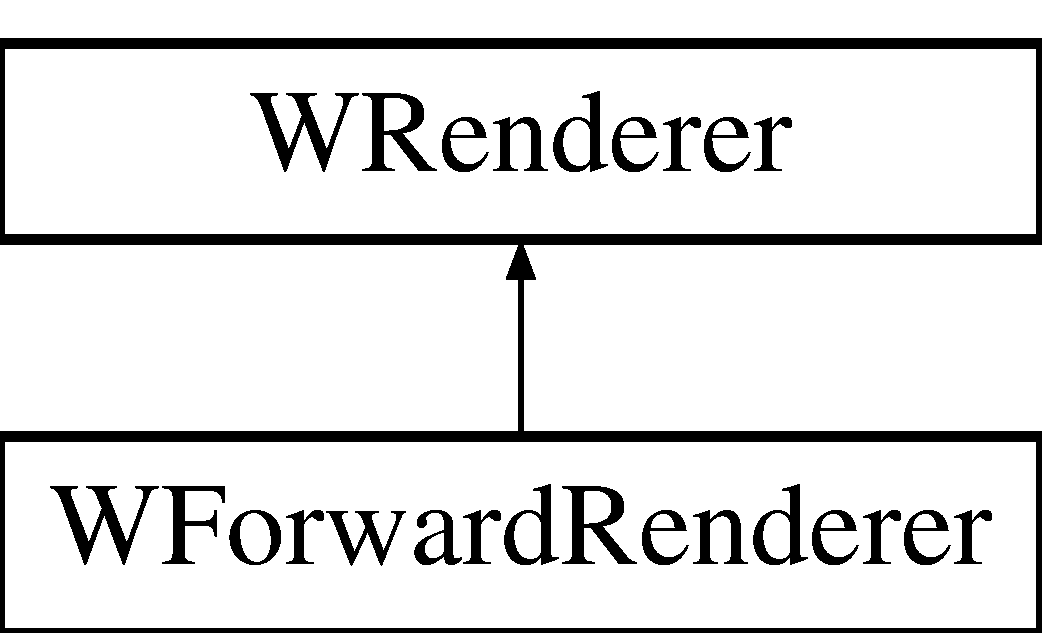
\includegraphics[height=2.000000cm]{class_w_forward_renderer}
\end{center}
\end{figure}
\subsection*{Public Member Functions}
\begin{DoxyCompactItemize}
\item 
{\bfseries W\+Forward\+Renderer} (class \hyperlink{class_wasabi}{Wasabi} $\ast$const app)\hypertarget{class_w_forward_renderer_a5153c67bdb9b27ca6cb683332f4cea9c}{}\label{class_w_forward_renderer_a5153c67bdb9b27ca6cb683332f4cea9c}

\item 
virtual \hyperlink{class_w_error}{W\+Error} {\bfseries Initiailize} ()\hypertarget{class_w_forward_renderer_a629fa8adb89dace7868ba870206ac5f0}{}\label{class_w_forward_renderer_a629fa8adb89dace7868ba870206ac5f0}

\item 
virtual void {\bfseries Render} (class \hyperlink{class_w_render_target}{W\+Render\+Target} $\ast$rt, unsigned int filter=-\/1)\hypertarget{class_w_forward_renderer_a69b90655513cd29f21c1dea9b2a1b706}{}\label{class_w_forward_renderer_a69b90655513cd29f21c1dea9b2a1b706}

\item 
virtual void {\bfseries Cleanup} ()\hypertarget{class_w_forward_renderer_a54e3da7b8e7b57fc7f20c82f43d6519b}{}\label{class_w_forward_renderer_a54e3da7b8e7b57fc7f20c82f43d6519b}

\item 
virtual \hyperlink{class_w_error}{W\+Error} {\bfseries Resize} (unsigned int width, unsigned int height)\hypertarget{class_w_forward_renderer_ace5e40731639f412ee0c1989b5e750e0}{}\label{class_w_forward_renderer_ace5e40731639f412ee0c1989b5e750e0}

\item 
virtual class \hyperlink{class_w_material}{W\+Material} $\ast$ {\bfseries Create\+Default\+Material} ()\hypertarget{class_w_forward_renderer_a54c58c8760eee602d9838db91c55be58}{}\label{class_w_forward_renderer_a54c58c8760eee602d9838db91c55be58}

\item 
virtual Vk\+Sampler {\bfseries Get\+Default\+Sampler} () const \hypertarget{class_w_forward_renderer_a0be96132cc36349dcfa6d71cdb846ffd}{}\label{class_w_forward_renderer_a0be96132cc36349dcfa6d71cdb846ffd}

\end{DoxyCompactItemize}
\subsection*{Friends}
\begin{DoxyCompactItemize}
\item 
class {\bfseries W\+F\+R\+Material}\hypertarget{class_w_forward_renderer_ad8978519eb6a5884691ce33a6c0b33ee}{}\label{class_w_forward_renderer_ad8978519eb6a5884691ce33a6c0b33ee}

\end{DoxyCompactItemize}
\subsection*{Additional Inherited Members}


The documentation for this class was generated from the following files\+:\begin{DoxyCompactItemize}
\item 
Wasabi/\+Renderers/W\+Forward\+Renderer.\+h\item 
Wasabi/\+Renderers/W\+Forward\+Renderer.\+cpp\end{DoxyCompactItemize}

\hypertarget{class_w_f_r_material}{}\section{W\+F\+R\+Material Class Reference}
\label{class_w_f_r_material}\index{W\+F\+R\+Material@{W\+F\+R\+Material}}
Inheritance diagram for W\+F\+R\+Material\+:\begin{figure}[H]
\begin{center}
\leavevmode
\includegraphics[height=3.000000cm]{class_w_f_r_material}
\end{center}
\end{figure}
\subsection*{Public Member Functions}
\begin{DoxyCompactItemize}
\item 
{\bfseries W\+F\+R\+Material} (class \hyperlink{class_wasabi}{Wasabi} $\ast$const app, unsigned int ID=0)\hypertarget{class_w_f_r_material_a870f81f67384798616d72ef0bf4228d5}{}\label{class_w_f_r_material_a870f81f67384798616d72ef0bf4228d5}

\item 
virtual \hyperlink{class_w_error}{W\+Error} \hyperlink{class_w_f_r_material_ab57a021a6e21d2c6dc872d6ea4450093}{Bind} (class \hyperlink{class_w_render_target}{W\+Render\+Target} $\ast$rt, unsigned int num\+\_\+vertex\+\_\+buffers=-\/1)
\item 
\hyperlink{class_w_error}{W\+Error} {\bfseries Texture} (class \hyperlink{class_w_image}{W\+Image} $\ast$img)\hypertarget{class_w_f_r_material_acc4467bcda7cc98023847549541bd0eb}{}\label{class_w_f_r_material_acc4467bcda7cc98023847549541bd0eb}

\item 
\hyperlink{class_w_error}{W\+Error} {\bfseries Set\+Color} (\hyperlink{class_w_color}{W\+Color} col)\hypertarget{class_w_f_r_material_a934ef9d40c49b7bc0faea7c941746520}{}\label{class_w_f_r_material_a934ef9d40c49b7bc0faea7c941746520}

\end{DoxyCompactItemize}
\subsection*{Additional Inherited Members}


\subsection{Member Function Documentation}
\index{W\+F\+R\+Material@{W\+F\+R\+Material}!Bind@{Bind}}
\index{Bind@{Bind}!W\+F\+R\+Material@{W\+F\+R\+Material}}
\subsubsection[{\texorpdfstring{Bind(class W\+Render\+Target $\ast$rt, unsigned int num\+\_\+vertex\+\_\+buffers=-\/1)}{Bind(class WRenderTarget *rt, unsigned int num_vertex_buffers=-1)}}]{\setlength{\rightskip}{0pt plus 5cm}{\bf W\+Error} W\+F\+R\+Material\+::\+Bind (
\begin{DoxyParamCaption}
\item[{class {\bf W\+Render\+Target} $\ast$}]{rt, }
\item[{unsigned int}]{num\+\_\+vertex\+\_\+buffers = {\ttfamily -\/1}}
\end{DoxyParamCaption}
)\hspace{0.3cm}{\ttfamily [virtual]}}\hypertarget{class_w_f_r_material_ab57a021a6e21d2c6dc872d6ea4450093}{}\label{class_w_f_r_material_ab57a021a6e21d2c6dc872d6ea4450093}
Binds the material and its effect to the graphics pipeline. A child class may choose to override this to change the binding procedure, or apply a certain operation upon binding. The render target must have its Begin() function called before this function is called. 
\begin{DoxyParams}{Parameters}
{\em rt} & Render target whose pipeline is being used \\
\hline
{\em num\+\_\+vertex\+\_\+buffers} & Number of vertex buffers that the material needs to render, valid values are either 0 if the effect uses no vertex buffers, or 1 to the number of input layouts in the effect \\
\hline
\end{DoxyParams}
\begin{DoxyReturn}{Returns}
Error code, see \hyperlink{_w_error_8h}{W\+Error.\+h} 
\end{DoxyReturn}


Reimplemented from \hyperlink{class_w_material_a420e012110ddabf5410bab0805fac025}{W\+Material}.



The documentation for this class was generated from the following files\+:\begin{DoxyCompactItemize}
\item 
Wasabi/\+Renderers/W\+Forward\+Renderer.\+h\item 
Wasabi/\+Renderers/W\+Forward\+Renderer.\+cpp\end{DoxyCompactItemize}

\hypertarget{class_w_game_state}{}\section{W\+Game\+State Class Reference}
\label{class_w_game_state}\index{W\+Game\+State@{W\+Game\+State}}


{\ttfamily \#include $<$W\+Core.\+h$>$}

Inheritance diagram for W\+Game\+State\+:\begin{figure}[H]
\begin{center}
\leavevmode
\includegraphics[height=2.000000cm]{class_w_game_state}
\end{center}
\end{figure}
\subsection*{Public Member Functions}
\begin{DoxyCompactItemize}
\item 
{\bfseries W\+Game\+State} (\hyperlink{class_wasabi}{Wasabi} $\ast$const a)\hypertarget{class_w_game_state_a2aa62cdf3a1dc59558b4aa017abdb248}{}\label{class_w_game_state_a2aa62cdf3a1dc59558b4aa017abdb248}

\item 
virtual void \hyperlink{class_w_game_state_a20031e5724a12eb99aa81c013d1d9d63}{Load} ()
\item 
virtual void \hyperlink{class_w_game_state_a5fe5a485ca56800cfd79237be2568d36}{Update} (float f\+Delta\+Time)
\item 
virtual void \hyperlink{class_w_game_state_ac4d0979d5ae27a8fd5df34949ae51d23}{On\+Keydown} (char c)
\item 
virtual void \hyperlink{class_w_game_state_abcae0b58bf3c27406f0783c628a3c714}{On\+Keyup} (char c)
\item 
virtual void \hyperlink{class_w_game_state_a952d55f104f8503f717ecbdcd6a8711c}{On\+Input} (char c)
\item 
virtual void \hyperlink{class_w_game_state_a50eddb2f648dc478ed0e10fee73fd4e9}{Cleanup} ()
\end{DoxyCompactItemize}
\subsection*{Protected Attributes}
\begin{DoxyCompactItemize}
\item 
\hyperlink{class_wasabi}{Wasabi} $\ast$const \hyperlink{class_w_game_state_a68c0b595d15be38854585e6cbcbe452b}{m\+\_\+app}
\end{DoxyCompactItemize}


\subsection{Detailed Description}
This class represents a game state. Game states can be used to completely separate different phases of a game. For example, one can crate a game state for the pre-\/menu credits, a state for the game menu and a state for the actual game.

States need to be allocated and freed by the user. 

\subsection{Member Function Documentation}
\index{W\+Game\+State@{W\+Game\+State}!Cleanup@{Cleanup}}
\index{Cleanup@{Cleanup}!W\+Game\+State@{W\+Game\+State}}
\subsubsection[{\texorpdfstring{Cleanup()}{Cleanup()}}]{\setlength{\rightskip}{0pt plus 5cm}virtual void W\+Game\+State\+::\+Cleanup (
\begin{DoxyParamCaption}
{}
\end{DoxyParamCaption}
)\hspace{0.3cm}{\ttfamily [inline]}, {\ttfamily [virtual]}}\hypertarget{class_w_game_state_a50eddb2f648dc478ed0e10fee73fd4e9}{}\label{class_w_game_state_a50eddb2f648dc478ed0e10fee73fd4e9}
This function is called before this state is switched from. This gives the state a chance to clean up its resources before its destroyed. 

Reimplemented in \hyperlink{class_instancing_demo_a5c8e4cc00517e928128771f91028d473}{Instancing\+Demo}, \hyperlink{class_animation_demo_a07d34d2c7f61565ac911d30216a9fb25}{Animation\+Demo}, and \hyperlink{class_kofta_a6650b02967c26d871e27aefd551e0c40}{Kofta}.

\index{W\+Game\+State@{W\+Game\+State}!Load@{Load}}
\index{Load@{Load}!W\+Game\+State@{W\+Game\+State}}
\subsubsection[{\texorpdfstring{Load()}{Load()}}]{\setlength{\rightskip}{0pt plus 5cm}virtual void W\+Game\+State\+::\+Load (
\begin{DoxyParamCaption}
{}
\end{DoxyParamCaption}
)\hspace{0.3cm}{\ttfamily [inline]}, {\ttfamily [virtual]}}\hypertarget{class_w_game_state_a20031e5724a12eb99aa81c013d1d9d63}{}\label{class_w_game_state_a20031e5724a12eb99aa81c013d1d9d63}
This function, will be called every time this state is switched to. This gives the state a chance to load its resources. 

Reimplemented in \hyperlink{class_instancing_demo_abf05a0b6ce3814cb50cc43785f0f53c8}{Instancing\+Demo}, \hyperlink{class_animation_demo_aec31e9f0100b86674561ba14e16f364d}{Animation\+Demo}, and \hyperlink{class_kofta_a82e99828dc080cbc5a9cfc3db7b50081}{Kofta}.

\index{W\+Game\+State@{W\+Game\+State}!On\+Input@{On\+Input}}
\index{On\+Input@{On\+Input}!W\+Game\+State@{W\+Game\+State}}
\subsubsection[{\texorpdfstring{On\+Input(char c)}{OnInput(char c)}}]{\setlength{\rightskip}{0pt plus 5cm}virtual void W\+Game\+State\+::\+On\+Input (
\begin{DoxyParamCaption}
\item[{char}]{c}
\end{DoxyParamCaption}
)\hspace{0.3cm}{\ttfamily [inline]}, {\ttfamily [virtual]}}\hypertarget{class_w_game_state_a952d55f104f8503f717ecbdcd6a8711c}{}\label{class_w_game_state_a952d55f104f8503f717ecbdcd6a8711c}
This function is called whenever character input is received while this state is active. Character input is supplied by the OS, and is best suitable for capturing input for things like text boxes. 
\begin{DoxyParams}{Parameters}
{\em c} & \mbox{[}description\mbox{]} \\
\hline
\end{DoxyParams}
\index{W\+Game\+State@{W\+Game\+State}!On\+Keydown@{On\+Keydown}}
\index{On\+Keydown@{On\+Keydown}!W\+Game\+State@{W\+Game\+State}}
\subsubsection[{\texorpdfstring{On\+Keydown(char c)}{OnKeydown(char c)}}]{\setlength{\rightskip}{0pt plus 5cm}virtual void W\+Game\+State\+::\+On\+Keydown (
\begin{DoxyParamCaption}
\item[{char}]{c}
\end{DoxyParamCaption}
)\hspace{0.3cm}{\ttfamily [inline]}, {\ttfamily [virtual]}}\hypertarget{class_w_game_state_ac4d0979d5ae27a8fd5df34949ae51d23}{}\label{class_w_game_state_ac4d0979d5ae27a8fd5df34949ae51d23}
This function is called whenever a key is pushed down while this state is active. 
\begin{DoxyParams}{Parameters}
{\em c} & The pushed key \\
\hline
\end{DoxyParams}
\index{W\+Game\+State@{W\+Game\+State}!On\+Keyup@{On\+Keyup}}
\index{On\+Keyup@{On\+Keyup}!W\+Game\+State@{W\+Game\+State}}
\subsubsection[{\texorpdfstring{On\+Keyup(char c)}{OnKeyup(char c)}}]{\setlength{\rightskip}{0pt plus 5cm}virtual void W\+Game\+State\+::\+On\+Keyup (
\begin{DoxyParamCaption}
\item[{char}]{c}
\end{DoxyParamCaption}
)\hspace{0.3cm}{\ttfamily [inline]}, {\ttfamily [virtual]}}\hypertarget{class_w_game_state_abcae0b58bf3c27406f0783c628a3c714}{}\label{class_w_game_state_abcae0b58bf3c27406f0783c628a3c714}
This function is called whenever a key is released while this state is active. 
\begin{DoxyParams}{Parameters}
{\em c} & The released key \\
\hline
\end{DoxyParams}
\index{W\+Game\+State@{W\+Game\+State}!Update@{Update}}
\index{Update@{Update}!W\+Game\+State@{W\+Game\+State}}
\subsubsection[{\texorpdfstring{Update(float f\+Delta\+Time)}{Update(float fDeltaTime)}}]{\setlength{\rightskip}{0pt plus 5cm}virtual void W\+Game\+State\+::\+Update (
\begin{DoxyParamCaption}
\item[{float}]{f\+Delta\+Time}
\end{DoxyParamCaption}
)\hspace{0.3cm}{\ttfamily [inline]}, {\ttfamily [virtual]}}\hypertarget{class_w_game_state_a5fe5a485ca56800cfd79237be2568d36}{}\label{class_w_game_state_a5fe5a485ca56800cfd79237be2568d36}
This function is called every frame (right after \hyperlink{class_wasabi_ae7f699787307843fc886c4a9a09ebab7}{Wasabi\+::\+Loop()}) while the state is active. 
\begin{DoxyParams}{Parameters}
{\em f\+Delta\+Time} & The step time for this frame (roughly 1 / F\+PS) \\
\hline
\end{DoxyParams}


Reimplemented in \hyperlink{class_instancing_demo_a233c7a0d4552fc6a4c8f43a59b04f01c}{Instancing\+Demo}, \hyperlink{class_animation_demo_aa694b73bfa77098e98a77399655203c2}{Animation\+Demo}, and \hyperlink{class_kofta_a27da31ebb583a8a017061823ab6575da}{Kofta}.



\subsection{Member Data Documentation}
\index{W\+Game\+State@{W\+Game\+State}!m\+\_\+app@{m\+\_\+app}}
\index{m\+\_\+app@{m\+\_\+app}!W\+Game\+State@{W\+Game\+State}}
\subsubsection[{\texorpdfstring{m\+\_\+app}{m_app}}]{\setlength{\rightskip}{0pt plus 5cm}{\bf Wasabi}$\ast$ const W\+Game\+State\+::m\+\_\+app\hspace{0.3cm}{\ttfamily [protected]}}\hypertarget{class_w_game_state_a68c0b595d15be38854585e6cbcbe452b}{}\label{class_w_game_state_a68c0b595d15be38854585e6cbcbe452b}
Pointer to the application (the \hyperlink{class_wasabi}{Wasabi} instance) 

The documentation for this class was generated from the following file\+:\begin{DoxyCompactItemize}
\item 
Wasabi/\+Core/\hyperlink{_w_core_8h}{W\+Core.\+h}\end{DoxyCompactItemize}

\hypertarget{class_w_geometry}{}\section{W\+Geometry Class Reference}
\label{class_w_geometry}\index{W\+Geometry@{W\+Geometry}}


{\ttfamily \#include $<$W\+Geometry.\+h$>$}

Inheritance diagram for W\+Geometry\+:\begin{figure}[H]
\begin{center}
\leavevmode
\includegraphics[height=3.000000cm]{class_w_geometry}
\end{center}
\end{figure}
\subsection*{Public Member Functions}
\begin{DoxyCompactItemize}
\item 
{\bfseries W\+Geometry} (\hyperlink{class_wasabi}{Wasabi} $\ast$const app, unsigned int ID=0)\hypertarget{class_w_geometry_a5bd75d5b0a5d557a09fd6565ea709fa1}{}\label{class_w_geometry_a5bd75d5b0a5d557a09fd6565ea709fa1}

\item 
virtual unsigned int \hyperlink{class_w_geometry_a4eab34844955ef4583d393c3304d250c}{Get\+Vertex\+Buffer\+Count} () const 
\item 
virtual \hyperlink{struct_w___v_e_r_t_e_x___d_e_s_c_r_i_p_t_i_o_n}{W\+\_\+\+V\+E\+R\+T\+E\+X\+\_\+\+D\+E\+S\+C\+R\+I\+P\+T\+I\+ON} \hyperlink{class_w_geometry_a84409cef0ba8228b571f4f69cdfd6131}{Get\+Vertex\+Description} (unsigned int layout\+\_\+index=0) const 
\item 
\hyperlink{class_w_error}{W\+Error} \hyperlink{class_w_geometry_ae9c73db37d16327132921df70669c6a4}{Create\+From\+Data} (void $\ast$vb, unsigned int num\+\_\+verts, void $\ast$ib, unsigned int num\+\_\+indices, bool b\+Dynamic=false, bool b\+Calc\+Normals=false, bool b\+Calc\+Tangents=false)
\item 
\hyperlink{class_w_error}{W\+Error} \hyperlink{class_w_geometry_a72d2e175081e0c3545497c621b8e4c95}{Create\+Cube} (float f\+Size, bool b\+Dynamic=false)
\item 
\hyperlink{class_w_error}{W\+Error} \hyperlink{class_w_geometry_a26ded3a7e2db75d132857d608e914bb0}{Create\+Box} (\hyperlink{class_w_vector3}{W\+Vector3} dimensions, bool b\+Dynamic=false)
\item 
\hyperlink{class_w_error}{W\+Error} \hyperlink{class_w_geometry_adeb899c32ca3f634dfccf7ba9780a3b3}{Create\+Plain} (float f\+Size, int xsegs, int zsegs, bool b\+Dynamic=false)
\item 
\hyperlink{class_w_error}{W\+Error} \hyperlink{class_w_geometry_a2a1d9a7ca9310f4e024250c33ace1dec}{Create\+Sphere} (float Radius, unsigned int V\+Res, unsigned int U\+Res, bool b\+Dynamic=false)
\item 
\hyperlink{class_w_error}{W\+Error} \hyperlink{class_w_geometry_a650d1bb17b2347329430925cc5e4aa86}{Create\+Cone} (float f\+Radius, float f\+Height, unsigned int hsegs, unsigned int csegs, bool b\+Dynamic=false)
\item 
\hyperlink{class_w_error}{W\+Error} \hyperlink{class_w_geometry_a312684c5e5f15629065c0e64fb8d121d}{Create\+Cylinder} (float f\+Radius, float f\+Height, unsigned int hsegs, unsigned int csegs, bool b\+Dynamic=false)
\item 
\hyperlink{class_w_error}{W\+Error} \hyperlink{class_w_geometry_afa735adb0739f6d54f467957168cfe38}{Copy\+From} (\hyperlink{class_w_geometry}{W\+Geometry} $\ast$const from, bool b\+Dynamic=false)
\item 
\hyperlink{class_w_error}{W\+Error} \hyperlink{class_w_geometry_a38749309af4f87d44d120bd978a12d90}{Create\+Animation\+Data} (void $\ast$anim\+Buf)
\item 
\hyperlink{class_w_error}{W\+Error} \hyperlink{class_w_geometry_afdffc9bd3c60a54d0d7875d7bf794ec2}{Load\+From\+W\+GM} (std\+::string filename, bool b\+Dynamic=false)
\item 
\hyperlink{class_w_error}{W\+Error} \hyperlink{class_w_geometry_a3e8135b72f0dc4b5f88204a070032c37}{Save\+To\+W\+GM} (std\+::string filename)
\item 
\hyperlink{class_w_error}{W\+Error} \hyperlink{class_w_geometry_a973bc874b7c22956f6dde88526e424bd}{Load\+From\+H\+XM} (std\+::string filename, bool b\+Dynamic=false)
\item 
\hyperlink{class_w_error}{W\+Error} \hyperlink{class_w_geometry_aa6618d489cf8fb3bbd8339ca16a620f1}{Map\+Vertex\+Buffer} (void $\ast$$\ast$const vb, bool b\+Read\+Only=false)
\item 
\hyperlink{class_w_error}{W\+Error} \hyperlink{class_w_geometry_a257228fd6ef4ca9c3ef7e86367be373d}{Map\+Index\+Buffer} (D\+W\+O\+RD $\ast$$\ast$const ib, bool b\+Read\+Only=false)
\item 
\hyperlink{class_w_error}{W\+Error} \hyperlink{class_w_geometry_ada2184692d09980547e6161226ccd51a}{Map\+Animation\+Buffer} (void $\ast$$\ast$const ab, bool b\+Read\+Only=false)
\item 
void \hyperlink{class_w_geometry_a39cf160839dcc25a35abc37bff873e8d}{Unmap\+Vertex\+Buffer} ()
\item 
void \hyperlink{class_w_geometry_ab543762e369709e5779694544f088286}{Unmap\+Index\+Buffer} ()
\item 
void \hyperlink{class_w_geometry_a33d5aa6e31d8d94baf37924c6dec51c9}{Unmap\+Animation\+Buffer} ()
\item 
\hyperlink{class_w_error}{W\+Error} \hyperlink{class_w_geometry_a83dd8a5914b6d5f8a204569885e3de63}{Scale} (float mul\+Factor)
\item 
\hyperlink{class_w_error}{W\+Error} \hyperlink{class_w_geometry_a4a7b0d5cbf2b708c9088b09286243871}{ScaleX} (float mul\+Factor)
\item 
\hyperlink{class_w_error}{W\+Error} \hyperlink{class_w_geometry_a4f55df8af86e43abd9e1a636d738ab9f}{ScaleY} (float mul\+Factor)
\item 
\hyperlink{class_w_error}{W\+Error} \hyperlink{class_w_geometry_a02aa684a0c9c53ae48a1e986686fff5b}{ScaleZ} (float mul\+Factor)
\item 
\hyperlink{class_w_error}{W\+Error} \hyperlink{class_w_geometry_a6d39140a33e39efad863c5804191ea3a}{Apply\+Offset} (float x, float y, float z)
\item 
\hyperlink{class_w_error}{W\+Error} \hyperlink{class_w_geometry_aebdd5369d14cdea3b2d213bfe8712ab9}{Apply\+Offset} (\hyperlink{class_w_vector3}{W\+Vector3} offset)
\item 
\hyperlink{class_w_error}{W\+Error} \hyperlink{class_w_geometry_a4aed0389d4630cf9e511cdcf757ea0a5}{Apply\+Transformation} (\hyperlink{class_w_matrix}{W\+Matrix} mtx)
\item 
bool \hyperlink{class_w_geometry_a63ea1ccc4bab8fb3ce70027ffd07626a}{Intersect} (\hyperlink{class_w_vector3}{W\+Vector3} p1, \hyperlink{class_w_vector3}{W\+Vector3} p2, \hyperlink{class_w_vector3}{W\+Vector3} $\ast$pt=nullptr, \hyperlink{class_w_vector2}{W\+Vector2} $\ast$uv=nullptr, unsigned int $\ast$triangle\+Index=nullptr)
\item 
\hyperlink{class_w_error}{W\+Error} \hyperlink{class_w_geometry_abf8e134f4345d4d998f9def43883f896}{Draw} (class \hyperlink{class_w_render_target}{W\+Render\+Target} $\ast$rt, unsigned int num\+\_\+triangles=-\/1, unsigned int num\+\_\+instances=1, bool bind\+\_\+animation=true)
\item 
\hyperlink{class_w_vector3}{W\+Vector3} \hyperlink{class_w_geometry_ab653f03a8e45a8474854e0dac3492d22}{Get\+Min\+Point} () const 
\item 
\hyperlink{class_w_vector3}{W\+Vector3} \hyperlink{class_w_geometry_a664b638b12cf086bf0774e4a6cb8a269}{Get\+Max\+Point} () const 
\item 
unsigned int \hyperlink{class_w_geometry_a174c95642aeff57b8baf47834d4b1ad7}{Get\+Num\+Vertices} () const 
\item 
unsigned int \hyperlink{class_w_geometry_a1aa307f3449402a1ff4aa82c73eeb502}{Get\+Num\+Indices} () const 
\item 
bool \hyperlink{class_w_geometry_a80d7625563854a50bd7de6aa7fdd9b3d}{Is\+Rigged} () const 
\item 
virtual bool \hyperlink{class_w_geometry_a41dcdf044d27efa83ff631c4921f9008}{Valid} () const 
\end{DoxyCompactItemize}
\subsection*{Additional Inherited Members}


\subsection{Detailed Description}
A \hyperlink{class_w_geometry}{W\+Geometry} is a flexible way to represent any geometry that is needed for rendering or any general computation or usage. \hyperlink{class_w_geometry}{W\+Geometry} can be derived such that one can modify the composition of the geometry (the attributes).

A geometry can be made immutable, making it use less memory, at the cost of having several functions not work (functions that require access to the geometry\textquotesingle{}s vertex data).

\hyperlink{class_w_geometry}{W\+Geometry} can hold several vertex buffers. By default, \hyperlink{class_wasabi}{Wasabi} uses the first buffer to render (with indices) and uses the second buffer (if available) for animation data. 

\subsection{Member Function Documentation}
\index{W\+Geometry@{W\+Geometry}!Apply\+Offset@{Apply\+Offset}}
\index{Apply\+Offset@{Apply\+Offset}!W\+Geometry@{W\+Geometry}}
\subsubsection[{\texorpdfstring{Apply\+Offset(float x, float y, float z)}{ApplyOffset(float x, float y, float z)}}]{\setlength{\rightskip}{0pt plus 5cm}{\bf W\+Error} W\+Geometry\+::\+Apply\+Offset (
\begin{DoxyParamCaption}
\item[{float}]{x, }
\item[{float}]{y, }
\item[{float}]{z}
\end{DoxyParamCaption}
)}\hypertarget{class_w_geometry_a6d39140a33e39efad863c5804191ea3a}{}\label{class_w_geometry_a6d39140a33e39efad863c5804191ea3a}
Applies an offset to all vertices in the geometry. The geometry must be valid and must have an attribute in its geometry buffer named \char`\"{}position\char`\"{}. The geometry must be dynamic and not immutable. 
\begin{DoxyParams}{Parameters}
{\em x} & x offset to apply \\
\hline
{\em y} & y offset to apply \\
\hline
{\em z} & z offset to apply \\
\hline
\end{DoxyParams}
\begin{DoxyReturn}{Returns}
Error code, see \hyperlink{_w_error_8h}{W\+Error.\+h} 
\end{DoxyReturn}
\index{W\+Geometry@{W\+Geometry}!Apply\+Offset@{Apply\+Offset}}
\index{Apply\+Offset@{Apply\+Offset}!W\+Geometry@{W\+Geometry}}
\subsubsection[{\texorpdfstring{Apply\+Offset(\+W\+Vector3 offset)}{ApplyOffset(WVector3 offset)}}]{\setlength{\rightskip}{0pt plus 5cm}{\bf W\+Error} W\+Geometry\+::\+Apply\+Offset (
\begin{DoxyParamCaption}
\item[{{\bf W\+Vector3}}]{offset}
\end{DoxyParamCaption}
)}\hypertarget{class_w_geometry_aebdd5369d14cdea3b2d213bfe8712ab9}{}\label{class_w_geometry_aebdd5369d14cdea3b2d213bfe8712ab9}
Applies an offset to all vertices in the geometry. The geometry must be valid and must have an attribute in its geometry buffer named \char`\"{}position\char`\"{}. The geometry must be dynamic and not immutable. 
\begin{DoxyParams}{Parameters}
{\em offset} & Offset to apply \\
\hline
\end{DoxyParams}
\begin{DoxyReturn}{Returns}
Error code, see \hyperlink{_w_error_8h}{W\+Error.\+h} 
\end{DoxyReturn}
\index{W\+Geometry@{W\+Geometry}!Apply\+Transformation@{Apply\+Transformation}}
\index{Apply\+Transformation@{Apply\+Transformation}!W\+Geometry@{W\+Geometry}}
\subsubsection[{\texorpdfstring{Apply\+Transformation(\+W\+Matrix mtx)}{ApplyTransformation(WMatrix mtx)}}]{\setlength{\rightskip}{0pt plus 5cm}{\bf W\+Error} W\+Geometry\+::\+Apply\+Transformation (
\begin{DoxyParamCaption}
\item[{{\bf W\+Matrix}}]{mtx}
\end{DoxyParamCaption}
)}\hypertarget{class_w_geometry_a4aed0389d4630cf9e511cdcf757ea0a5}{}\label{class_w_geometry_a4aed0389d4630cf9e511cdcf757ea0a5}
Applies a transformation matrix to all vertices in the geometry. The geometry must be valid and must have an attribute in its geometry buffer named \char`\"{}position\char`\"{}. The geometry must be dynamic and not immutable. 
\begin{DoxyParams}{Parameters}
{\em mtx} & Transformation matrix to apply \\
\hline
\end{DoxyParams}
\begin{DoxyReturn}{Returns}
Error code, see \hyperlink{_w_error_8h}{W\+Error.\+h} 
\end{DoxyReturn}
\index{W\+Geometry@{W\+Geometry}!Copy\+From@{Copy\+From}}
\index{Copy\+From@{Copy\+From}!W\+Geometry@{W\+Geometry}}
\subsubsection[{\texorpdfstring{Copy\+From(\+W\+Geometry $\ast$const from, bool b\+Dynamic=false)}{CopyFrom(WGeometry *const from, bool bDynamic=false)}}]{\setlength{\rightskip}{0pt plus 5cm}{\bf W\+Error} W\+Geometry\+::\+Copy\+From (
\begin{DoxyParamCaption}
\item[{{\bf W\+Geometry} $\ast$const}]{from, }
\item[{bool}]{b\+Dynamic = {\ttfamily false}}
\end{DoxyParamCaption}
)}\hypertarget{class_w_geometry_afa735adb0739f6d54f467957168cfe38}{}\label{class_w_geometry_afa735adb0739f6d54f467957168cfe38}
Copy another (non-\/immutable) geometry.

If this function is called while the engine parameter \char`\"{}geometry\+Immutable\char`\"{} (see \hyperlink{class_wasabi_ab3d3e87ba206b4184b504c1666ff6dc3}{Wasabi\+::engine\+Params}) is set to true, then the geometry will be made immutable, regardless of the b\+Dynamic parameter. Immutable geometry cannot have the following function calls work\+: \hyperlink{class_w_geometry_a3e8135b72f0dc4b5f88204a070032c37}{Save\+To\+W\+G\+M()}, all map and unmap functions, all scaling functions, all offset functions and \hyperlink{class_w_geometry_a63ea1ccc4bab8fb3ce70027ffd07626a}{Intersect()}. Immutable geometry cannot be copied. Immutable geometry uses less memory.


\begin{DoxyParams}{Parameters}
{\em from} & Geometry to copy \\
\hline
{\em b\+Dynamic} & true if the geometry will require frequent modifications, false otherwise \\
\hline
\end{DoxyParams}
\begin{DoxyReturn}{Returns}
Error code, see \hyperlink{_w_error_8h}{W\+Error.\+h} 
\end{DoxyReturn}
\index{W\+Geometry@{W\+Geometry}!Create\+Animation\+Data@{Create\+Animation\+Data}}
\index{Create\+Animation\+Data@{Create\+Animation\+Data}!W\+Geometry@{W\+Geometry}}
\subsubsection[{\texorpdfstring{Create\+Animation\+Data(void $\ast$anim\+Buf)}{CreateAnimationData(void *animBuf)}}]{\setlength{\rightskip}{0pt plus 5cm}{\bf W\+Error} W\+Geometry\+::\+Create\+Animation\+Data (
\begin{DoxyParamCaption}
\item[{void $\ast$}]{anim\+Buf}
\end{DoxyParamCaption}
)}\hypertarget{class_w_geometry_a38749309af4f87d44d120bd978a12d90}{}\label{class_w_geometry_a38749309af4f87d44d120bd978a12d90}
Creates animation data vertex buffer. The geometry must have \hyperlink{class_w_geometry_a4eab34844955ef4583d393c3304d250c}{Get\+Vertex\+Buffer\+Count()} $>$ 1. The buffer will be dynamic if the first vertex buffer (created from a Load$\ast$, \hyperlink{class_w_geometry_ae9c73db37d16327132921df70669c6a4}{Create\+From\+Data()} or \hyperlink{class_w_geometry_afa735adb0739f6d54f467957168cfe38}{Copy\+From()} call) was dynamic, false otherwise. If the geometry of this object is immutable, the the animation buffer will also be.


\begin{DoxyParams}{Parameters}
{\em anim\+Buf} & A pointer to the memory to create the animation buffer from, which must be a valid contiguous memory of size \hyperlink{class_w_geometry_a174c95642aeff57b8baf47834d4b1ad7}{Get\+Num\+Vertices()}$\ast$\+Get\+Vertex\+Description(1).Get\+Size() \\
\hline
\end{DoxyParams}
\begin{DoxyReturn}{Returns}
Error code, see \hyperlink{_w_error_8h}{W\+Error.\+h} 
\end{DoxyReturn}
\index{W\+Geometry@{W\+Geometry}!Create\+Box@{Create\+Box}}
\index{Create\+Box@{Create\+Box}!W\+Geometry@{W\+Geometry}}
\subsubsection[{\texorpdfstring{Create\+Box(\+W\+Vector3 dimensions, bool b\+Dynamic=false)}{CreateBox(WVector3 dimensions, bool bDynamic=false)}}]{\setlength{\rightskip}{0pt plus 5cm}{\bf W\+Error} W\+Geometry\+::\+Create\+Box (
\begin{DoxyParamCaption}
\item[{{\bf W\+Vector3}}]{dimensions, }
\item[{bool}]{b\+Dynamic = {\ttfamily false}}
\end{DoxyParamCaption}
)}\hypertarget{class_w_geometry_a26ded3a7e2db75d132857d608e914bb0}{}\label{class_w_geometry_a26ded3a7e2db75d132857d608e914bb0}
Creates a box geometry.

If this function is called while the engine parameter \char`\"{}geometry\+Immutable\char`\"{} (see \hyperlink{class_wasabi_ab3d3e87ba206b4184b504c1666ff6dc3}{Wasabi\+::engine\+Params}) is set to true, then the geometry will be made immutable, regardless of the b\+Dynamic parameter. Immutable geometry cannot have the following function calls work\+: \hyperlink{class_w_geometry_a3e8135b72f0dc4b5f88204a070032c37}{Save\+To\+W\+G\+M()}, all map and unmap functions, all scaling functions, all offset functions and \hyperlink{class_w_geometry_a63ea1ccc4bab8fb3ce70027ffd07626a}{Intersect()}. Immutable geometry cannot be copied. Immutable geometry uses less memory.


\begin{DoxyParams}{Parameters}
{\em dimensions} & Dimensions of the box \\
\hline
{\em b\+Dynamic} & true if the geometry will require frequent modifications, false otherwise \\
\hline
\end{DoxyParams}
\begin{DoxyReturn}{Returns}
Error code, see \hyperlink{_w_error_8h}{W\+Error.\+h} 
\end{DoxyReturn}
\index{W\+Geometry@{W\+Geometry}!Create\+Cone@{Create\+Cone}}
\index{Create\+Cone@{Create\+Cone}!W\+Geometry@{W\+Geometry}}
\subsubsection[{\texorpdfstring{Create\+Cone(float f\+Radius, float f\+Height, unsigned int hsegs, unsigned int csegs, bool b\+Dynamic=false)}{CreateCone(float fRadius, float fHeight, unsigned int hsegs, unsigned int csegs, bool bDynamic=false)}}]{\setlength{\rightskip}{0pt plus 5cm}{\bf W\+Error} W\+Geometry\+::\+Create\+Cone (
\begin{DoxyParamCaption}
\item[{float}]{f\+Radius, }
\item[{float}]{f\+Height, }
\item[{unsigned int}]{hsegs, }
\item[{unsigned int}]{csegs, }
\item[{bool}]{b\+Dynamic = {\ttfamily false}}
\end{DoxyParamCaption}
)}\hypertarget{class_w_geometry_a650d1bb17b2347329430925cc5e4aa86}{}\label{class_w_geometry_a650d1bb17b2347329430925cc5e4aa86}
Creates a cone geometry, with csegs segments at the bottom circle and hsegs segments along the cone\textquotesingle{}s height.

If this function is called while the engine parameter \char`\"{}geometry\+Immutable\char`\"{} (see \hyperlink{class_wasabi_ab3d3e87ba206b4184b504c1666ff6dc3}{Wasabi\+::engine\+Params}) is set to true, then the geometry will be made immutable, regardless of the b\+Dynamic parameter. Immutable geometry cannot have the following function calls work\+: \hyperlink{class_w_geometry_a3e8135b72f0dc4b5f88204a070032c37}{Save\+To\+W\+G\+M()}, all map and unmap functions, all scaling functions, all offset functions and \hyperlink{class_w_geometry_a63ea1ccc4bab8fb3ce70027ffd07626a}{Intersect()}. Immutable geometry cannot be copied. Immutable geometry uses less memory.


\begin{DoxyParams}{Parameters}
{\em f\+Radius} & Radius of the bottom circle \\
\hline
{\em f\+Height} & Height of the cone \\
\hline
{\em hsegs} & Number of segments along the height, minimum is 0 \\
\hline
{\em csegs} & Number of segments at the bottom circle, minimum is 3 \\
\hline
{\em b\+Dynamic} & true if the geometry will require frequent modifications, false otherwise \\
\hline
\end{DoxyParams}
\begin{DoxyReturn}{Returns}
Error code, see \hyperlink{_w_error_8h}{W\+Error.\+h} 
\end{DoxyReturn}
\index{W\+Geometry@{W\+Geometry}!Create\+Cube@{Create\+Cube}}
\index{Create\+Cube@{Create\+Cube}!W\+Geometry@{W\+Geometry}}
\subsubsection[{\texorpdfstring{Create\+Cube(float f\+Size, bool b\+Dynamic=false)}{CreateCube(float fSize, bool bDynamic=false)}}]{\setlength{\rightskip}{0pt plus 5cm}{\bf W\+Error} W\+Geometry\+::\+Create\+Cube (
\begin{DoxyParamCaption}
\item[{float}]{f\+Size, }
\item[{bool}]{b\+Dynamic = {\ttfamily false}}
\end{DoxyParamCaption}
)}\hypertarget{class_w_geometry_a72d2e175081e0c3545497c621b8e4c95}{}\label{class_w_geometry_a72d2e175081e0c3545497c621b8e4c95}
Creates a cube geometry.

If this function is called while the engine parameter \char`\"{}geometry\+Immutable\char`\"{} (see \hyperlink{class_wasabi_ab3d3e87ba206b4184b504c1666ff6dc3}{Wasabi\+::engine\+Params}) is set to true, then the geometry will be made immutable, regardless of the b\+Dynamic parameter. Immutable geometry cannot have the following function calls work\+: \hyperlink{class_w_geometry_a3e8135b72f0dc4b5f88204a070032c37}{Save\+To\+W\+G\+M()}, all map and unmap functions, all scaling functions, all offset functions and \hyperlink{class_w_geometry_a63ea1ccc4bab8fb3ce70027ffd07626a}{Intersect()}. Immutable geometry cannot be copied. Immutable geometry uses less memory.


\begin{DoxyParams}{Parameters}
{\em f\+Size} & Dimension of the cube \\
\hline
{\em b\+Dynamic} & true if the geometry will require frequent modifications, false otherwise \\
\hline
\end{DoxyParams}
\begin{DoxyReturn}{Returns}
Error code, see \hyperlink{_w_error_8h}{W\+Error.\+h} 
\end{DoxyReturn}
\index{W\+Geometry@{W\+Geometry}!Create\+Cylinder@{Create\+Cylinder}}
\index{Create\+Cylinder@{Create\+Cylinder}!W\+Geometry@{W\+Geometry}}
\subsubsection[{\texorpdfstring{Create\+Cylinder(float f\+Radius, float f\+Height, unsigned int hsegs, unsigned int csegs, bool b\+Dynamic=false)}{CreateCylinder(float fRadius, float fHeight, unsigned int hsegs, unsigned int csegs, bool bDynamic=false)}}]{\setlength{\rightskip}{0pt plus 5cm}{\bf W\+Error} W\+Geometry\+::\+Create\+Cylinder (
\begin{DoxyParamCaption}
\item[{float}]{f\+Radius, }
\item[{float}]{f\+Height, }
\item[{unsigned int}]{hsegs, }
\item[{unsigned int}]{csegs, }
\item[{bool}]{b\+Dynamic = {\ttfamily false}}
\end{DoxyParamCaption}
)}\hypertarget{class_w_geometry_a312684c5e5f15629065c0e64fb8d121d}{}\label{class_w_geometry_a312684c5e5f15629065c0e64fb8d121d}
Creates a cylinder geometry, with csegs segments at the bottom and top circles and hsegs segments along the cylinder\textquotesingle{}s height.

If this function is called while the engine parameter \char`\"{}geometry\+Immutable\char`\"{} (see \hyperlink{class_wasabi_ab3d3e87ba206b4184b504c1666ff6dc3}{Wasabi\+::engine\+Params}) is set to true, then the geometry will be made immutable, regardless of the b\+Dynamic parameter. Immutable geometry cannot have the following function calls work\+: \hyperlink{class_w_geometry_a3e8135b72f0dc4b5f88204a070032c37}{Save\+To\+W\+G\+M()}, all map and unmap functions, all scaling functions, all offset functions and \hyperlink{class_w_geometry_a63ea1ccc4bab8fb3ce70027ffd07626a}{Intersect()}. Immutable geometry cannot be copied. Immutable geometry uses less memory.


\begin{DoxyParams}{Parameters}
{\em f\+Radius} & Radius of the cylinder \\
\hline
{\em f\+Height} & Height of the cylinder \\
\hline
{\em hsegs} & Number of segments along the height, minimum is 0 \\
\hline
{\em csegs} & Number of segments at the bottom and top circles, minimum is 3 \\
\hline
{\em b\+Dynamic} & true if the geometry will require frequent modifications, false otherwise \\
\hline
\end{DoxyParams}
\begin{DoxyReturn}{Returns}
Error code, see \hyperlink{_w_error_8h}{W\+Error.\+h} 
\end{DoxyReturn}
\index{W\+Geometry@{W\+Geometry}!Create\+From\+Data@{Create\+From\+Data}}
\index{Create\+From\+Data@{Create\+From\+Data}!W\+Geometry@{W\+Geometry}}
\subsubsection[{\texorpdfstring{Create\+From\+Data(void $\ast$vb, unsigned int num\+\_\+verts, void $\ast$ib, unsigned int num\+\_\+indices, bool b\+Dynamic=false, bool b\+Calc\+Normals=false, bool b\+Calc\+Tangents=false)}{CreateFromData(void *vb, unsigned int num_verts, void *ib, unsigned int num_indices, bool bDynamic=false, bool bCalcNormals=false, bool bCalcTangents=false)}}]{\setlength{\rightskip}{0pt plus 5cm}{\bf W\+Error} W\+Geometry\+::\+Create\+From\+Data (
\begin{DoxyParamCaption}
\item[{void $\ast$}]{vb, }
\item[{unsigned int}]{num\+\_\+verts, }
\item[{void $\ast$}]{ib, }
\item[{unsigned int}]{num\+\_\+indices, }
\item[{bool}]{b\+Dynamic = {\ttfamily false}, }
\item[{bool}]{b\+Calc\+Normals = {\ttfamily false}, }
\item[{bool}]{b\+Calc\+Tangents = {\ttfamily false}}
\end{DoxyParamCaption}
)}\hypertarget{class_w_geometry_ae9c73db37d16327132921df70669c6a4}{}\label{class_w_geometry_ae9c73db37d16327132921df70669c6a4}
Creates a geometry from buffers in memory. The buffers must be formatted such that they match what \hyperlink{class_w_geometry_a84409cef0ba8228b571f4f69cdfd6131}{Get\+Vertex\+Description()} returns. This function fills up only the first (0th) vertex buffer that is accompanied with an index buffer for rendering use.

If this function is called while the engine parameter \char`\"{}geometry\+Immutable\char`\"{} (see \hyperlink{class_wasabi_ab3d3e87ba206b4184b504c1666ff6dc3}{Wasabi\+::engine\+Params}) is set to true, then the geometry will be made immutable, regardless of the b\+Dynamic parameter. Immutable geometry cannot have the following function calls work\+: \hyperlink{class_w_geometry_a3e8135b72f0dc4b5f88204a070032c37}{Save\+To\+W\+G\+M()}, all map and unmap functions, all scaling functions, all offset functions and \hyperlink{class_w_geometry_a63ea1ccc4bab8fb3ce70027ffd07626a}{Intersect()}. Immutable geometry cannot be copied. Immutable geometry uses less memory.

Examples\+: Create a triangle\+: 
\begin{DoxyCode}
\hyperlink{struct_w_default_vertex}{WDefaultVertex} vertices[] = \{
  \hyperlink{struct_w_default_vertex}{WDefaultVertex}(-0.5f, -0.5f, 0.0f, 1.0f, 0.0f, 0.0f,
                 0.0f, 0.0f, -1.0f, 0.0f, 1.0f),
  \hyperlink{struct_w_default_vertex}{WDefaultVertex}(-0.5f, 0.5f, 0.0f, 1.0f, 0.0f, 0.0f,
                 0.0f, 0.0f, -1.0f, 0.0f, 0.0f),
  \hyperlink{struct_w_default_vertex}{WDefaultVertex}(0.5f, 0.5f, 0.0f, 1.0f, 0.0f, 0.0f,
                 0.0f, 0.0f, -1.0f, 1.0f, 0.0f)
\};
DWORD indices[] = \{0, 1, 2\};
WGeomery* geometry = \textcolor{keyword}{new} \hyperlink{class_w_geometry}{WGeometry}(\textcolor{keyword}{this});
geometry->CreateFromData(vertices, 3, indices, 3);
\end{DoxyCode}



\begin{DoxyParams}{Parameters}
{\em vb} & A pointer to the memory containing the vertex data, which must be a valid contiguous memory of size num\+\_\+verts$\ast$\+Get\+Vertex\+Description(0).Get\+Size() \\
\hline
{\em num\+\_\+verts} & Number of vertices in vb \\
\hline
{\em ib} & A pointer to the memory containing the index data, which must be a valid contiguous memory of size num\+\_\+indices$\ast$sizeof(D\+W\+O\+RD) \\
\hline
{\em num\+\_\+indices} & Number of indices in ab \\
\hline
{\em b\+Dynamic} & true if the geometry will require frequent modifications, false otherwise \\
\hline
{\em b\+Calc\+Normals} & Setting this to true will cause this function to automatically calculate normals (if there is an attribute named \char`\"{}normal\char`\"{} in Get\+Vertex\+Description(0)) for the geometry (hard-\/normals) \\
\hline
{\em b\+Calc\+Tangents} & Setting this to true will cause this function to automatically calculate tangents (if there is an attribute named \char`\"{}tangent\char`\"{} in Get\+Vertex\+Description(0)) for the geometry \\
\hline
\end{DoxyParams}
\begin{DoxyReturn}{Returns}
Error code, see \hyperlink{_w_error_8h}{W\+Error.\+h} 
\end{DoxyReturn}
\index{W\+Geometry@{W\+Geometry}!Create\+Plain@{Create\+Plain}}
\index{Create\+Plain@{Create\+Plain}!W\+Geometry@{W\+Geometry}}
\subsubsection[{\texorpdfstring{Create\+Plain(float f\+Size, int xsegs, int zsegs, bool b\+Dynamic=false)}{CreatePlain(float fSize, int xsegs, int zsegs, bool bDynamic=false)}}]{\setlength{\rightskip}{0pt plus 5cm}{\bf W\+Error} W\+Geometry\+::\+Create\+Plain (
\begin{DoxyParamCaption}
\item[{float}]{f\+Size, }
\item[{int}]{xsegs, }
\item[{int}]{zsegs, }
\item[{bool}]{b\+Dynamic = {\ttfamily false}}
\end{DoxyParamCaption}
)}\hypertarget{class_w_geometry_adeb899c32ca3f634dfccf7ba9780a3b3}{}\label{class_w_geometry_adeb899c32ca3f634dfccf7ba9780a3b3}
Creates a plain geometry that is segmented. The plain will be split into (xsegs+1)$\ast$(zsegs+1) squares, which will have 2 triangles each.

If this function is called while the engine parameter \char`\"{}geometry\+Immutable\char`\"{} (see \hyperlink{class_wasabi_ab3d3e87ba206b4184b504c1666ff6dc3}{Wasabi\+::engine\+Params}) is set to true, then the geometry will be made immutable, regardless of the b\+Dynamic parameter. Immutable geometry cannot have the following function calls work\+: \hyperlink{class_w_geometry_a3e8135b72f0dc4b5f88204a070032c37}{Save\+To\+W\+G\+M()}, all map and unmap functions, all scaling functions, all offset functions and \hyperlink{class_w_geometry_a63ea1ccc4bab8fb3ce70027ffd07626a}{Intersect()}. Immutable geometry cannot be copied. Immutable geometry uses less memory.


\begin{DoxyParams}{Parameters}
{\em f\+Size} & Size (dimension) of the plain \\
\hline
{\em xsegs} & Number of segments on the X axis, minimum is 0 \\
\hline
{\em zsegs} & Number of segments on the Z axis, minimum is 0 \\
\hline
{\em b\+Dynamic} & true if the geometry will require frequent modifications, false otherwise \\
\hline
\end{DoxyParams}
\begin{DoxyReturn}{Returns}
Error code, see \hyperlink{_w_error_8h}{W\+Error.\+h} 
\end{DoxyReturn}
\index{W\+Geometry@{W\+Geometry}!Create\+Sphere@{Create\+Sphere}}
\index{Create\+Sphere@{Create\+Sphere}!W\+Geometry@{W\+Geometry}}
\subsubsection[{\texorpdfstring{Create\+Sphere(float Radius, unsigned int V\+Res, unsigned int U\+Res, bool b\+Dynamic=false)}{CreateSphere(float Radius, unsigned int VRes, unsigned int URes, bool bDynamic=false)}}]{\setlength{\rightskip}{0pt plus 5cm}{\bf W\+Error} W\+Geometry\+::\+Create\+Sphere (
\begin{DoxyParamCaption}
\item[{float}]{Radius, }
\item[{unsigned int}]{V\+Res, }
\item[{unsigned int}]{U\+Res, }
\item[{bool}]{b\+Dynamic = {\ttfamily false}}
\end{DoxyParamCaption}
)}\hypertarget{class_w_geometry_a2a1d9a7ca9310f4e024250c33ace1dec}{}\label{class_w_geometry_a2a1d9a7ca9310f4e024250c33ace1dec}
Creates a sphere geometry, with V\+Res vertical segments and U\+Res horizontal segments.

If this function is called while the engine parameter \char`\"{}geometry\+Immutable\char`\"{} (see \hyperlink{class_wasabi_ab3d3e87ba206b4184b504c1666ff6dc3}{Wasabi\+::engine\+Params}) is set to true, then the geometry will be made immutable, regardless of the b\+Dynamic parameter. Immutable geometry cannot have the following function calls work\+: \hyperlink{class_w_geometry_a3e8135b72f0dc4b5f88204a070032c37}{Save\+To\+W\+G\+M()}, all map and unmap functions, all scaling functions, all offset functions and \hyperlink{class_w_geometry_a63ea1ccc4bab8fb3ce70027ffd07626a}{Intersect()}. Immutable geometry cannot be copied. Immutable geometry uses less memory.


\begin{DoxyParams}{Parameters}
{\em Radius} & Radius of the sphere \\
\hline
{\em V\+Res} & Vertical resolution, or number of vertical splits, minimum is 3 \\
\hline
{\em U\+Res} & Horizontal resolution, or number of horizontal splits, minimum is 2 \\
\hline
{\em b\+Dynamic} & true if the geometry will require frequent modifications, false otherwise \\
\hline
\end{DoxyParams}
\begin{DoxyReturn}{Returns}
Error code, see \hyperlink{_w_error_8h}{W\+Error.\+h} 
\end{DoxyReturn}
\index{W\+Geometry@{W\+Geometry}!Draw@{Draw}}
\index{Draw@{Draw}!W\+Geometry@{W\+Geometry}}
\subsubsection[{\texorpdfstring{Draw(class W\+Render\+Target $\ast$rt, unsigned int num\+\_\+triangles=-\/1, unsigned int num\+\_\+instances=1, bool bind\+\_\+animation=true)}{Draw(class WRenderTarget *rt, unsigned int num_triangles=-1, unsigned int num_instances=1, bool bind_animation=true)}}]{\setlength{\rightskip}{0pt plus 5cm}{\bf W\+Error} W\+Geometry\+::\+Draw (
\begin{DoxyParamCaption}
\item[{class {\bf W\+Render\+Target} $\ast$}]{rt, }
\item[{unsigned int}]{num\+\_\+triangles = {\ttfamily -\/1}, }
\item[{unsigned int}]{num\+\_\+instances = {\ttfamily 1}, }
\item[{bool}]{bind\+\_\+animation = {\ttfamily true}}
\end{DoxyParamCaption}
)}\hypertarget{class_w_geometry_abf8e134f4345d4d998f9def43883f896}{}\label{class_w_geometry_abf8e134f4345d4d998f9def43883f896}
Draw the geometry to the render target. This function will bind the geometry buffer to vertex buffer slot 0 in Vulkan, and will bind the animation buffer (if available and requested) to slot 1. The render target must have its Begin() function called before this function is called. 
\begin{DoxyParams}{Parameters}
{\em rt} & Render target to draw to \\
\hline
{\em num\+\_\+triangles} & Number of triangles to draw, -\/1 for all \\
\hline
{\em num\+\_\+instances} & Number of instances to draw \\
\hline
{\em bind\+\_\+animation} & true to bind the animation buffer (if not available, the geometry buffer will be bound twice), false otherwise \\
\hline
\end{DoxyParams}
\begin{DoxyReturn}{Returns}
\mbox{[}description\mbox{]} 
\end{DoxyReturn}
\index{W\+Geometry@{W\+Geometry}!Get\+Max\+Point@{Get\+Max\+Point}}
\index{Get\+Max\+Point@{Get\+Max\+Point}!W\+Geometry@{W\+Geometry}}
\subsubsection[{\texorpdfstring{Get\+Max\+Point() const }{GetMaxPoint() const }}]{\setlength{\rightskip}{0pt plus 5cm}{\bf W\+Vector3} W\+Geometry\+::\+Get\+Max\+Point (
\begin{DoxyParamCaption}
{}
\end{DoxyParamCaption}
) const}\hypertarget{class_w_geometry_a664b638b12cf086bf0774e4a6cb8a269}{}\label{class_w_geometry_a664b638b12cf086bf0774e4a6cb8a269}
Retrieves the point that represents the maximum boundary of the geometry. \begin{DoxyReturn}{Returns}
The maximum boundary for the geometry 
\end{DoxyReturn}
\index{W\+Geometry@{W\+Geometry}!Get\+Min\+Point@{Get\+Min\+Point}}
\index{Get\+Min\+Point@{Get\+Min\+Point}!W\+Geometry@{W\+Geometry}}
\subsubsection[{\texorpdfstring{Get\+Min\+Point() const }{GetMinPoint() const }}]{\setlength{\rightskip}{0pt plus 5cm}{\bf W\+Vector3} W\+Geometry\+::\+Get\+Min\+Point (
\begin{DoxyParamCaption}
{}
\end{DoxyParamCaption}
) const}\hypertarget{class_w_geometry_ab653f03a8e45a8474854e0dac3492d22}{}\label{class_w_geometry_ab653f03a8e45a8474854e0dac3492d22}
Retrieves the point that represents the minimum boundary of the geometry. \begin{DoxyReturn}{Returns}
The minimum boundary for the geometry 
\end{DoxyReturn}
\index{W\+Geometry@{W\+Geometry}!Get\+Num\+Indices@{Get\+Num\+Indices}}
\index{Get\+Num\+Indices@{Get\+Num\+Indices}!W\+Geometry@{W\+Geometry}}
\subsubsection[{\texorpdfstring{Get\+Num\+Indices() const }{GetNumIndices() const }}]{\setlength{\rightskip}{0pt plus 5cm}unsigned int W\+Geometry\+::\+Get\+Num\+Indices (
\begin{DoxyParamCaption}
{}
\end{DoxyParamCaption}
) const}\hypertarget{class_w_geometry_a1aa307f3449402a1ff4aa82c73eeb502}{}\label{class_w_geometry_a1aa307f3449402a1ff4aa82c73eeb502}
Retrieves the number of indices in the geometry. \begin{DoxyReturn}{Returns}
Number of indices 
\end{DoxyReturn}
\index{W\+Geometry@{W\+Geometry}!Get\+Num\+Vertices@{Get\+Num\+Vertices}}
\index{Get\+Num\+Vertices@{Get\+Num\+Vertices}!W\+Geometry@{W\+Geometry}}
\subsubsection[{\texorpdfstring{Get\+Num\+Vertices() const }{GetNumVertices() const }}]{\setlength{\rightskip}{0pt plus 5cm}unsigned int W\+Geometry\+::\+Get\+Num\+Vertices (
\begin{DoxyParamCaption}
{}
\end{DoxyParamCaption}
) const}\hypertarget{class_w_geometry_a174c95642aeff57b8baf47834d4b1ad7}{}\label{class_w_geometry_a174c95642aeff57b8baf47834d4b1ad7}
Retrieves the number of vertices in the geometry. \begin{DoxyReturn}{Returns}
Number of vertices 
\end{DoxyReturn}
\index{W\+Geometry@{W\+Geometry}!Get\+Vertex\+Buffer\+Count@{Get\+Vertex\+Buffer\+Count}}
\index{Get\+Vertex\+Buffer\+Count@{Get\+Vertex\+Buffer\+Count}!W\+Geometry@{W\+Geometry}}
\subsubsection[{\texorpdfstring{Get\+Vertex\+Buffer\+Count() const }{GetVertexBufferCount() const }}]{\setlength{\rightskip}{0pt plus 5cm}virtual unsigned int W\+Geometry\+::\+Get\+Vertex\+Buffer\+Count (
\begin{DoxyParamCaption}
{}
\end{DoxyParamCaption}
) const\hspace{0.3cm}{\ttfamily [inline]}, {\ttfamily [virtual]}}\hypertarget{class_w_geometry_a4eab34844955ef4583d393c3304d250c}{}\label{class_w_geometry_a4eab34844955ef4583d393c3304d250c}
This function should return the number of vertex descriptions that \hyperlink{class_w_geometry_a84409cef0ba8228b571f4f69cdfd6131}{Get\+Vertex\+Description()} can return, which represents the number of vertex buffers this geometry class can hold. \begin{DoxyReturn}{Returns}
The number of vertex buffers this geometry can hold 
\end{DoxyReturn}


Reimplemented in \hyperlink{class_text_geometry_a0d6f019bc0034edcfdb51fe743e3b681}{Text\+Geometry}, and \hyperlink{class_sprite_geometry_a3c2a4c34292f6643f4bc7f375fe7ae68}{Sprite\+Geometry}.

\index{W\+Geometry@{W\+Geometry}!Get\+Vertex\+Description@{Get\+Vertex\+Description}}
\index{Get\+Vertex\+Description@{Get\+Vertex\+Description}!W\+Geometry@{W\+Geometry}}
\subsubsection[{\texorpdfstring{Get\+Vertex\+Description(unsigned int layout\+\_\+index=0) const }{GetVertexDescription(unsigned int layout_index=0) const }}]{\setlength{\rightskip}{0pt plus 5cm}virtual {\bf W\+\_\+\+V\+E\+R\+T\+E\+X\+\_\+\+D\+E\+S\+C\+R\+I\+P\+T\+I\+ON} W\+Geometry\+::\+Get\+Vertex\+Description (
\begin{DoxyParamCaption}
\item[{unsigned int}]{layout\+\_\+index = {\ttfamily 0}}
\end{DoxyParamCaption}
) const\hspace{0.3cm}{\ttfamily [inline]}, {\ttfamily [virtual]}}\hypertarget{class_w_geometry_a84409cef0ba8228b571f4f69cdfd6131}{}\label{class_w_geometry_a84409cef0ba8228b571f4f69cdfd6131}
Retrieves the vertex description of a vertex buffer. Should return valid descriptions for all {\itshape layout\+\_\+index} values between 0 and \hyperlink{class_w_geometry_a4eab34844955ef4583d393c3304d250c}{Get\+Vertex\+Buffer\+Count()}-\/1. 
\begin{DoxyParams}{Parameters}
{\em layout\+\_\+index} & Index of the vertex buffer \\
\hline
\end{DoxyParams}
\begin{DoxyReturn}{Returns}
The description of a vertex in the layout\+\_\+index \textquotesingle{}th vertex buffer 
\end{DoxyReturn}


Reimplemented in \hyperlink{class_text_geometry_a048ec440054230443d89317dd09d2731}{Text\+Geometry}, and \hyperlink{class_sprite_geometry_a84172139912969ed1d36f48506f5918a}{Sprite\+Geometry}.

\index{W\+Geometry@{W\+Geometry}!Intersect@{Intersect}}
\index{Intersect@{Intersect}!W\+Geometry@{W\+Geometry}}
\subsubsection[{\texorpdfstring{Intersect(\+W\+Vector3 p1, W\+Vector3 p2, W\+Vector3 $\ast$pt=nullptr, W\+Vector2 $\ast$uv=nullptr, unsigned int $\ast$triangle\+Index=nullptr)}{Intersect(WVector3 p1, WVector3 p2, WVector3 *pt=nullptr, WVector2 *uv=nullptr, unsigned int *triangleIndex=nullptr)}}]{\setlength{\rightskip}{0pt plus 5cm}bool W\+Geometry\+::\+Intersect (
\begin{DoxyParamCaption}
\item[{{\bf W\+Vector3}}]{p1, }
\item[{{\bf W\+Vector3}}]{p2, }
\item[{{\bf W\+Vector3} $\ast$}]{pt = {\ttfamily nullptr}, }
\item[{{\bf W\+Vector2} $\ast$}]{uv = {\ttfamily nullptr}, }
\item[{unsigned int $\ast$}]{triangle\+Index = {\ttfamily nullptr}}
\end{DoxyParamCaption}
)}\hypertarget{class_w_geometry_a63ea1ccc4bab8fb3ce70027ffd07626a}{}\label{class_w_geometry_a63ea1ccc4bab8fb3ce70027ffd07626a}
Checks if a ray intersects the geometry. The geometry must be valid and must have an attribute in its geometry buffer named \char`\"{}position\char`\"{}. The geometry must be dynamic and not immutable. 
\begin{DoxyParams}{Parameters}
{\em p1} & Origin of the ray \\
\hline
{\em p2} & A vector that points in the same direction as the ray \\
\hline
{\em pt} & A pointer to a 3D vector to be populated with the point of intersection, if any \\
\hline
{\em uv} & A pointer to a 2D vector to be populated with the UV coordinates at the intersection point, if any. If the vertices don\textquotesingle{}t have a an attribute named uv (with at least two components) then this will be the UV coordinates local to the triangle intersected \\
\hline
{\em triangle\+Index} & A pointer to an integer to be populated with the index of the triangle that was intersected, if any \\
\hline
\end{DoxyParams}
\begin{DoxyReturn}{Returns}
true if there was an intersection, false otherwise 
\end{DoxyReturn}
\index{W\+Geometry@{W\+Geometry}!Is\+Rigged@{Is\+Rigged}}
\index{Is\+Rigged@{Is\+Rigged}!W\+Geometry@{W\+Geometry}}
\subsubsection[{\texorpdfstring{Is\+Rigged() const }{IsRigged() const }}]{\setlength{\rightskip}{0pt plus 5cm}bool W\+Geometry\+::\+Is\+Rigged (
\begin{DoxyParamCaption}
{}
\end{DoxyParamCaption}
) const}\hypertarget{class_w_geometry_a80d7625563854a50bd7de6aa7fdd9b3d}{}\label{class_w_geometry_a80d7625563854a50bd7de6aa7fdd9b3d}
Checks if the geometry has an animation vertex buffer. \begin{DoxyReturn}{Returns}
true if the geometry has animation data, false otherwise 
\end{DoxyReturn}
\index{W\+Geometry@{W\+Geometry}!Load\+From\+H\+XM@{Load\+From\+H\+XM}}
\index{Load\+From\+H\+XM@{Load\+From\+H\+XM}!W\+Geometry@{W\+Geometry}}
\subsubsection[{\texorpdfstring{Load\+From\+H\+X\+M(std\+::string filename, bool b\+Dynamic=false)}{LoadFromHXM(std::string filename, bool bDynamic=false)}}]{\setlength{\rightskip}{0pt plus 5cm}{\bf W\+Error} W\+Geometry\+::\+Load\+From\+H\+XM (
\begin{DoxyParamCaption}
\item[{std\+::string}]{filename, }
\item[{bool}]{b\+Dynamic = {\ttfamily false}}
\end{DoxyParamCaption}
)}\hypertarget{class_w_geometry_a973bc874b7c22956f6dde88526e424bd}{}\label{class_w_geometry_a973bc874b7c22956f6dde88526e424bd}
Load a geometry from an H\+XM file. The geometry in the H\+XM file may be of a different format, in which case this function will try to fill in the attributes that the two formats share, discarding the rest. If no normal or tangent data are found in the file, but are available in this geometry\textquotesingle{}s description, the function will attempt to fill them in automatically. 
\begin{DoxyParams}{Parameters}
{\em filename} & Name of the file to load \\
\hline
{\em b\+Dynamic} & true if the geometry will require frequent modifications, false otherwise \\
\hline
\end{DoxyParams}
\begin{DoxyReturn}{Returns}
Error code, see \hyperlink{_w_error_8h}{W\+Error.\+h} 
\end{DoxyReturn}
\index{W\+Geometry@{W\+Geometry}!Load\+From\+W\+GM@{Load\+From\+W\+GM}}
\index{Load\+From\+W\+GM@{Load\+From\+W\+GM}!W\+Geometry@{W\+Geometry}}
\subsubsection[{\texorpdfstring{Load\+From\+W\+G\+M(std\+::string filename, bool b\+Dynamic=false)}{LoadFromWGM(std::string filename, bool bDynamic=false)}}]{\setlength{\rightskip}{0pt plus 5cm}{\bf W\+Error} W\+Geometry\+::\+Load\+From\+W\+GM (
\begin{DoxyParamCaption}
\item[{std\+::string}]{filename, }
\item[{bool}]{b\+Dynamic = {\ttfamily false}}
\end{DoxyParamCaption}
)}\hypertarget{class_w_geometry_afdffc9bd3c60a54d0d7875d7bf794ec2}{}\label{class_w_geometry_afdffc9bd3c60a54d0d7875d7bf794ec2}
Load a geometry from a W\+GM file. The geometry in the W\+GM file may be of a different format, in which case this function will try to fill in the attributes that the two formats share, discarding the rest. If no normal or tangent data are found in the file, but are available in this geometry\textquotesingle{}s description, the function will attempt to fill them in automatically. The function will also attempt to load animation data, if available. However, animation data will only be loaded if it matches exactly with this geometry\textquotesingle{}s animation vertex buffer structure. 
\begin{DoxyParams}{Parameters}
{\em filename} & Name of the file to load \\
\hline
{\em b\+Dynamic} & true if the geometry will require frequent modifications, false otherwise \\
\hline
\end{DoxyParams}
\begin{DoxyReturn}{Returns}
Error code, see \hyperlink{_w_error_8h}{W\+Error.\+h} 
\end{DoxyReturn}
\index{W\+Geometry@{W\+Geometry}!Map\+Animation\+Buffer@{Map\+Animation\+Buffer}}
\index{Map\+Animation\+Buffer@{Map\+Animation\+Buffer}!W\+Geometry@{W\+Geometry}}
\subsubsection[{\texorpdfstring{Map\+Animation\+Buffer(void $\ast$$\ast$const ab, bool b\+Read\+Only=false)}{MapAnimationBuffer(void **const ab, bool bReadOnly=false)}}]{\setlength{\rightskip}{0pt plus 5cm}{\bf W\+Error} W\+Geometry\+::\+Map\+Animation\+Buffer (
\begin{DoxyParamCaption}
\item[{void $\ast$$\ast$const}]{ab, }
\item[{bool}]{b\+Read\+Only = {\ttfamily false}}
\end{DoxyParamCaption}
)}\hypertarget{class_w_geometry_ada2184692d09980547e6161226ccd51a}{}\label{class_w_geometry_ada2184692d09980547e6161226ccd51a}
Map the animation buffer of this geometry. This will fail if there is no animation data, the geometry is dynamic or if the geometry is immutable. 
\begin{DoxyParams}{Parameters}
{\em ab} & The address of a pointer to have it point to the mapped memory of the animation vertices \\
\hline
{\em b\+Read\+Only} & Set to true if you intend to only read from the animation vertex array, false if you want to modify the animation vertices \\
\hline
\end{DoxyParams}
\begin{DoxyReturn}{Returns}
Error code, see \hyperlink{_w_error_8h}{W\+Error.\+h} 
\end{DoxyReturn}
\index{W\+Geometry@{W\+Geometry}!Map\+Index\+Buffer@{Map\+Index\+Buffer}}
\index{Map\+Index\+Buffer@{Map\+Index\+Buffer}!W\+Geometry@{W\+Geometry}}
\subsubsection[{\texorpdfstring{Map\+Index\+Buffer(\+D\+W\+O\+R\+D $\ast$$\ast$const ib, bool b\+Read\+Only=false)}{MapIndexBuffer(DWORD **const ib, bool bReadOnly=false)}}]{\setlength{\rightskip}{0pt plus 5cm}{\bf W\+Error} W\+Geometry\+::\+Map\+Index\+Buffer (
\begin{DoxyParamCaption}
\item[{D\+W\+O\+RD $\ast$$\ast$const}]{ib, }
\item[{bool}]{b\+Read\+Only = {\ttfamily false}}
\end{DoxyParamCaption}
)}\hypertarget{class_w_geometry_a257228fd6ef4ca9c3ef7e86367be373d}{}\label{class_w_geometry_a257228fd6ef4ca9c3ef7e86367be373d}
Map the index buffer of this geometry. This will fail if there is no geometry, the geometry is dynamic or if the geometry is immutable.

Examples\+: Flip this first triangle 
\begin{DoxyCode}
\textcolor{comment}{// Assuming geometry is valid and dynamic}
DWORD* indices;
geometry->MapIndexBuffer(&indices);
DWORD temp = indices[0];
indices[0] = indices[2];
indices[2] = temp;
geometry->UnmapIndexBuffer();
\end{DoxyCode}



\begin{DoxyParams}{Parameters}
{\em ib} & The address of a pointer to have it point to the mapped memory of the indices \\
\hline
{\em b\+Read\+Only} & Set to true if you intend to only read from the index array, false if you want to modify the indices \\
\hline
\end{DoxyParams}
\begin{DoxyReturn}{Returns}
Error code, see \hyperlink{_w_error_8h}{W\+Error.\+h} 
\end{DoxyReturn}
\index{W\+Geometry@{W\+Geometry}!Map\+Vertex\+Buffer@{Map\+Vertex\+Buffer}}
\index{Map\+Vertex\+Buffer@{Map\+Vertex\+Buffer}!W\+Geometry@{W\+Geometry}}
\subsubsection[{\texorpdfstring{Map\+Vertex\+Buffer(void $\ast$$\ast$const vb, bool b\+Read\+Only=false)}{MapVertexBuffer(void **const vb, bool bReadOnly=false)}}]{\setlength{\rightskip}{0pt plus 5cm}{\bf W\+Error} W\+Geometry\+::\+Map\+Vertex\+Buffer (
\begin{DoxyParamCaption}
\item[{void $\ast$$\ast$const}]{vb, }
\item[{bool}]{b\+Read\+Only = {\ttfamily false}}
\end{DoxyParamCaption}
)}\hypertarget{class_w_geometry_aa6618d489cf8fb3bbd8339ca16a620f1}{}\label{class_w_geometry_aa6618d489cf8fb3bbd8339ca16a620f1}
Map the vertex buffer of this geometry. This will fail if there is no geometry, the geometry is dynamic or if the geometry is immutable.

Examples\+: Move the first vertex a bit 
\begin{DoxyCode}
\textcolor{comment}{// Assuming geometry is valid and dynamic}
\hyperlink{struct_w_default_vertex}{WDefaultVertex}* vertices;
geometry->MapVertexBuffer((\textcolor{keywordtype}{void}**)&vertices);
vertices[0].\hyperlink{struct_w_default_vertex_afdcf7f42cc5581df2f6952aaf839e8bb}{pos}.\hyperlink{class_w_vector3_a79d057d696196227f92c35331efb9da7}{x} += 5;
geometry->UnmapVertexBuffer();
\end{DoxyCode}



\begin{DoxyParams}{Parameters}
{\em vb} & The address of a pointer to have it point to the mapped memory of the vertices \\
\hline
{\em b\+Read\+Only} & Set to true if you intend to only read from the vertex array, false if you want to modify the vertices \\
\hline
\end{DoxyParams}
\begin{DoxyReturn}{Returns}
Error code, see \hyperlink{_w_error_8h}{W\+Error.\+h} 
\end{DoxyReturn}
\index{W\+Geometry@{W\+Geometry}!Save\+To\+W\+GM@{Save\+To\+W\+GM}}
\index{Save\+To\+W\+GM@{Save\+To\+W\+GM}!W\+Geometry@{W\+Geometry}}
\subsubsection[{\texorpdfstring{Save\+To\+W\+G\+M(std\+::string filename)}{SaveToWGM(std::string filename)}}]{\setlength{\rightskip}{0pt plus 5cm}{\bf W\+Error} W\+Geometry\+::\+Save\+To\+W\+GM (
\begin{DoxyParamCaption}
\item[{std\+::string}]{filename}
\end{DoxyParamCaption}
)}\hypertarget{class_w_geometry_a3e8135b72f0dc4b5f88204a070032c37}{}\label{class_w_geometry_a3e8135b72f0dc4b5f88204a070032c37}
Saves this geometry\textquotesingle{}s data in a W\+GM file. The data will be saved in the same format of this geometry. Animation data will also be stored. 
\begin{DoxyParams}{Parameters}
{\em filename} & Name of the file \\
\hline
\end{DoxyParams}
\begin{DoxyReturn}{Returns}
Error code, see \hyperlink{_w_error_8h}{W\+Error.\+h} 
\end{DoxyReturn}
\index{W\+Geometry@{W\+Geometry}!Scale@{Scale}}
\index{Scale@{Scale}!W\+Geometry@{W\+Geometry}}
\subsubsection[{\texorpdfstring{Scale(float mul\+Factor)}{Scale(float mulFactor)}}]{\setlength{\rightskip}{0pt plus 5cm}{\bf W\+Error} W\+Geometry\+::\+Scale (
\begin{DoxyParamCaption}
\item[{float}]{mul\+Factor}
\end{DoxyParamCaption}
)}\hypertarget{class_w_geometry_a83dd8a5914b6d5f8a204569885e3de63}{}\label{class_w_geometry_a83dd8a5914b6d5f8a204569885e3de63}
Scale the geometry. The geometry must be valid and must have an attribute in its geometry buffer named \char`\"{}position\char`\"{}. The geometry must be dynamic and not immutable. 
\begin{DoxyParams}{Parameters}
{\em mul\+Factor} & Scale factor \\
\hline
\end{DoxyParams}
\begin{DoxyReturn}{Returns}
Error code, see \hyperlink{_w_error_8h}{W\+Error.\+h} 
\end{DoxyReturn}
\index{W\+Geometry@{W\+Geometry}!ScaleX@{ScaleX}}
\index{ScaleX@{ScaleX}!W\+Geometry@{W\+Geometry}}
\subsubsection[{\texorpdfstring{Scale\+X(float mul\+Factor)}{ScaleX(float mulFactor)}}]{\setlength{\rightskip}{0pt plus 5cm}{\bf W\+Error} W\+Geometry\+::\+ScaleX (
\begin{DoxyParamCaption}
\item[{float}]{mul\+Factor}
\end{DoxyParamCaption}
)}\hypertarget{class_w_geometry_a4a7b0d5cbf2b708c9088b09286243871}{}\label{class_w_geometry_a4a7b0d5cbf2b708c9088b09286243871}
Scale the geometry on the X axis. The geometry must be valid and must have an attribute in its geometry buffer named \char`\"{}position\char`\"{}. The geometry must be dynamic and not immutable. 
\begin{DoxyParams}{Parameters}
{\em mul\+Factor} & X scale factor \\
\hline
\end{DoxyParams}
\begin{DoxyReturn}{Returns}
Error code, see \hyperlink{_w_error_8h}{W\+Error.\+h} 
\end{DoxyReturn}
\index{W\+Geometry@{W\+Geometry}!ScaleY@{ScaleY}}
\index{ScaleY@{ScaleY}!W\+Geometry@{W\+Geometry}}
\subsubsection[{\texorpdfstring{Scale\+Y(float mul\+Factor)}{ScaleY(float mulFactor)}}]{\setlength{\rightskip}{0pt plus 5cm}{\bf W\+Error} W\+Geometry\+::\+ScaleY (
\begin{DoxyParamCaption}
\item[{float}]{mul\+Factor}
\end{DoxyParamCaption}
)}\hypertarget{class_w_geometry_a4f55df8af86e43abd9e1a636d738ab9f}{}\label{class_w_geometry_a4f55df8af86e43abd9e1a636d738ab9f}
Scale the geometry on the Y axis. The geometry must be valid and must have an attribute in its geometry buffer named \char`\"{}position\char`\"{}. The geometry must be dynamic and not immutable. 
\begin{DoxyParams}{Parameters}
{\em mul\+Factor} & Y scale factor \\
\hline
\end{DoxyParams}
\begin{DoxyReturn}{Returns}
Error code, see \hyperlink{_w_error_8h}{W\+Error.\+h} 
\end{DoxyReturn}
\index{W\+Geometry@{W\+Geometry}!ScaleZ@{ScaleZ}}
\index{ScaleZ@{ScaleZ}!W\+Geometry@{W\+Geometry}}
\subsubsection[{\texorpdfstring{Scale\+Z(float mul\+Factor)}{ScaleZ(float mulFactor)}}]{\setlength{\rightskip}{0pt plus 5cm}{\bf W\+Error} W\+Geometry\+::\+ScaleZ (
\begin{DoxyParamCaption}
\item[{float}]{mul\+Factor}
\end{DoxyParamCaption}
)}\hypertarget{class_w_geometry_a02aa684a0c9c53ae48a1e986686fff5b}{}\label{class_w_geometry_a02aa684a0c9c53ae48a1e986686fff5b}
Scale the geometry on the Z axis. The geometry must be valid and must have an attribute in its geometry buffer named \char`\"{}position\char`\"{}. The geometry must be dynamic and not immutable. 
\begin{DoxyParams}{Parameters}
{\em mul\+Factor} & Z scale factor \\
\hline
\end{DoxyParams}
\begin{DoxyReturn}{Returns}
Error code, see \hyperlink{_w_error_8h}{W\+Error.\+h} 
\end{DoxyReturn}
\index{W\+Geometry@{W\+Geometry}!Unmap\+Animation\+Buffer@{Unmap\+Animation\+Buffer}}
\index{Unmap\+Animation\+Buffer@{Unmap\+Animation\+Buffer}!W\+Geometry@{W\+Geometry}}
\subsubsection[{\texorpdfstring{Unmap\+Animation\+Buffer()}{UnmapAnimationBuffer()}}]{\setlength{\rightskip}{0pt plus 5cm}void W\+Geometry\+::\+Unmap\+Animation\+Buffer (
\begin{DoxyParamCaption}
{}
\end{DoxyParamCaption}
)}\hypertarget{class_w_geometry_a33d5aa6e31d8d94baf37924c6dec51c9}{}\label{class_w_geometry_a33d5aa6e31d8d94baf37924c6dec51c9}
Unmap animation vertices from a previous \hyperlink{class_w_geometry_ada2184692d09980547e6161226ccd51a}{Map\+Animation\+Buffer()} call. If \hyperlink{class_w_geometry_ada2184692d09980547e6161226ccd51a}{Map\+Animation\+Buffer()} was called with b\+Read\+Only == false, the this will apply the changes to the animation data. \index{W\+Geometry@{W\+Geometry}!Unmap\+Index\+Buffer@{Unmap\+Index\+Buffer}}
\index{Unmap\+Index\+Buffer@{Unmap\+Index\+Buffer}!W\+Geometry@{W\+Geometry}}
\subsubsection[{\texorpdfstring{Unmap\+Index\+Buffer()}{UnmapIndexBuffer()}}]{\setlength{\rightskip}{0pt plus 5cm}void W\+Geometry\+::\+Unmap\+Index\+Buffer (
\begin{DoxyParamCaption}
{}
\end{DoxyParamCaption}
)}\hypertarget{class_w_geometry_ab543762e369709e5779694544f088286}{}\label{class_w_geometry_ab543762e369709e5779694544f088286}
Unmap indices from a previous \hyperlink{class_w_geometry_a257228fd6ef4ca9c3ef7e86367be373d}{Map\+Index\+Buffer()} call. If \hyperlink{class_w_geometry_a257228fd6ef4ca9c3ef7e86367be373d}{Map\+Index\+Buffer()} was called with b\+Read\+Only == false, the this will apply the changes to the geometry. \index{W\+Geometry@{W\+Geometry}!Unmap\+Vertex\+Buffer@{Unmap\+Vertex\+Buffer}}
\index{Unmap\+Vertex\+Buffer@{Unmap\+Vertex\+Buffer}!W\+Geometry@{W\+Geometry}}
\subsubsection[{\texorpdfstring{Unmap\+Vertex\+Buffer()}{UnmapVertexBuffer()}}]{\setlength{\rightskip}{0pt plus 5cm}void W\+Geometry\+::\+Unmap\+Vertex\+Buffer (
\begin{DoxyParamCaption}
{}
\end{DoxyParamCaption}
)}\hypertarget{class_w_geometry_a39cf160839dcc25a35abc37bff873e8d}{}\label{class_w_geometry_a39cf160839dcc25a35abc37bff873e8d}
Unmap vertices from a previous \hyperlink{class_w_geometry_aa6618d489cf8fb3bbd8339ca16a620f1}{Map\+Vertex\+Buffer()} call. If \hyperlink{class_w_geometry_aa6618d489cf8fb3bbd8339ca16a620f1}{Map\+Vertex\+Buffer()} was called with b\+Read\+Only == false, the this will apply the changes to the geometry. \index{W\+Geometry@{W\+Geometry}!Valid@{Valid}}
\index{Valid@{Valid}!W\+Geometry@{W\+Geometry}}
\subsubsection[{\texorpdfstring{Valid() const }{Valid() const }}]{\setlength{\rightskip}{0pt plus 5cm}bool W\+Geometry\+::\+Valid (
\begin{DoxyParamCaption}
\item[{void}]{}
\end{DoxyParamCaption}
) const\hspace{0.3cm}{\ttfamily [virtual]}}\hypertarget{class_w_geometry_a41dcdf044d27efa83ff631c4921f9008}{}\label{class_w_geometry_a41dcdf044d27efa83ff631c4921f9008}
Checks the validity of the geometry. A geometry is valid if it has a vertex and an index buffer. \begin{DoxyReturn}{Returns}
true if the geometry is valid, false otherwise 
\end{DoxyReturn}


Implements \hyperlink{class_w_base_a76ac973ba9a43e182f6a6a4869d69725}{W\+Base}.



\subsection{Member Data Documentation}
\index{W\+Geometry@{W\+Geometry}!buffer@{buffer}}
\index{buffer@{buffer}!W\+Geometry@{W\+Geometry}}
\subsubsection[{\texorpdfstring{buffer}{buffer}}]{\setlength{\rightskip}{0pt plus 5cm}{\bf W\+\_\+\+B\+U\+F\+F\+ER} W\+Geometry\+::buffer}\hypertarget{class_w_geometry_a471c54efc2d9f3eca8de35f677deeede}{}\label{class_w_geometry_a471c54efc2d9f3eca8de35f677deeede}
Vertex buffer

Index buffer

Animation vertex buffer \index{W\+Geometry@{W\+Geometry}!count@{count}}
\index{count@{count}!W\+Geometry@{W\+Geometry}}
\subsubsection[{\texorpdfstring{count}{count}}]{\setlength{\rightskip}{0pt plus 5cm}int W\+Geometry\+::count}\hypertarget{class_w_geometry_a54ddd29ae6e2a476dcd1fbc4afe76116}{}\label{class_w_geometry_a54ddd29ae6e2a476dcd1fbc4afe76116}
Number of vertices

Number of indices \index{W\+Geometry@{W\+Geometry}!read\+Only\+Map@{read\+Only\+Map}}
\index{read\+Only\+Map@{read\+Only\+Map}!W\+Geometry@{W\+Geometry}}
\subsubsection[{\texorpdfstring{read\+Only\+Map}{readOnlyMap}}]{\setlength{\rightskip}{0pt plus 5cm}bool W\+Geometry\+::read\+Only\+Map}\hypertarget{class_w_geometry_acfbe406adf9413c67cf08a2d60061c5d}{}\label{class_w_geometry_acfbe406adf9413c67cf08a2d60061c5d}
Set to true if the last vertex map operation was read only

Set to true if the last index map operation was read only

Set to true if the last animation vertex map operation was read only \index{W\+Geometry@{W\+Geometry}!staging@{staging}}
\index{staging@{staging}!W\+Geometry@{W\+Geometry}}
\subsubsection[{\texorpdfstring{staging}{staging}}]{\setlength{\rightskip}{0pt plus 5cm}{\bf W\+\_\+\+B\+U\+F\+F\+ER} W\+Geometry\+::staging}\hypertarget{class_w_geometry_a270b11468a7492990fe3df154b981be5}{}\label{class_w_geometry_a270b11468a7492990fe3df154b981be5}
Staging vertex buffer, used for dynamic access

Staging index buffer, used for dynamic access

Staging animation vertex buffer, used for dynamic access 

The documentation for this class was generated from the following files\+:\begin{DoxyCompactItemize}
\item 
Wasabi/\+Geometries/\hyperlink{_w_geometry_8h}{W\+Geometry.\+h}\item 
Wasabi/\+Geometries/W\+Geometry.\+cpp\end{DoxyCompactItemize}

\hypertarget{class_w_geometry_manager}{}\section{W\+Geometry\+Manager Class Reference}
\label{class_w_geometry_manager}\index{W\+Geometry\+Manager@{W\+Geometry\+Manager}}


{\ttfamily \#include $<$W\+Geometry.\+h$>$}

Inheritance diagram for W\+Geometry\+Manager\+:\begin{figure}[H]
\begin{center}
\leavevmode
\includegraphics[height=2.000000cm]{class_w_geometry_manager}
\end{center}
\end{figure}
\subsection*{Public Member Functions}
\begin{DoxyCompactItemize}
\item 
{\bfseries W\+Geometry\+Manager} (class \hyperlink{class_wasabi}{Wasabi} $\ast$const app)\hypertarget{class_w_geometry_manager_aef4630cbfd7630f985091615f8e4a7f3}{}\label{class_w_geometry_manager_aef4630cbfd7630f985091615f8e4a7f3}

\end{DoxyCompactItemize}
\subsection*{Additional Inherited Members}


\subsection{Detailed Description}
Manager class for \hyperlink{class_w_geometry}{W\+Geometry}. 

The documentation for this class was generated from the following files\+:\begin{DoxyCompactItemize}
\item 
Wasabi/\+Geometries/\hyperlink{_w_geometry_8h}{W\+Geometry.\+h}\item 
Wasabi/\+Geometries/W\+Geometry.\+cpp\end{DoxyCompactItemize}

\hypertarget{class_w_havok_physics}{}\section{W\+Havok\+Physics Class Reference}
\label{class_w_havok_physics}\index{W\+Havok\+Physics@{W\+Havok\+Physics}}
Inheritance diagram for W\+Havok\+Physics\+:\begin{figure}[H]
\begin{center}
\leavevmode
\includegraphics[height=2.000000cm]{class_w_havok_physics}
\end{center}
\end{figure}
\subsection*{Public Member Functions}
\begin{DoxyCompactItemize}
\item 
{\bfseries W\+Havok\+Physics} (class \hyperlink{class_wasabi}{Wasabi} $\ast$app)\hypertarget{class_w_havok_physics_a93f39b8b7fb90aa15931095f36e8bd6f}{}\label{class_w_havok_physics_a93f39b8b7fb90aa15931095f36e8bd6f}

\item 
virtual \hyperlink{class_w_error}{W\+Error} {\bfseries Initialize} ()\hypertarget{class_w_havok_physics_a15ecfddee3f656b2c5b6363490207d42}{}\label{class_w_havok_physics_a15ecfddee3f656b2c5b6363490207d42}

\item 
virtual void {\bfseries Cleanup} ()\hypertarget{class_w_havok_physics_ad6f54f99bd16ec14cf605453050eb393}{}\label{class_w_havok_physics_ad6f54f99bd16ec14cf605453050eb393}

\item 
virtual void {\bfseries Start} ()\hypertarget{class_w_havok_physics_a39da923d35db5f5489601d034027a3db}{}\label{class_w_havok_physics_a39da923d35db5f5489601d034027a3db}

\item 
virtual void {\bfseries Stop} ()\hypertarget{class_w_havok_physics_a0f95216fddd7cde8fcda6e61ff6c1a10}{}\label{class_w_havok_physics_a0f95216fddd7cde8fcda6e61ff6c1a10}

\item 
virtual void {\bfseries Step} (float delta\+Time)\hypertarget{class_w_havok_physics_a8fde3cd7224124fda0ee7d7116e648ff}{}\label{class_w_havok_physics_a8fde3cd7224124fda0ee7d7116e648ff}

\item 
virtual bool {\bfseries Stepping} () const \hypertarget{class_w_havok_physics_ab5694d9003c22085d878c450b153db61}{}\label{class_w_havok_physics_ab5694d9003c22085d878c450b153db61}

\item 
virtual bool {\bfseries Ray\+Cast} (\hyperlink{class_w_vector3}{W\+Vector3} from, \hyperlink{class_w_vector3}{W\+Vector3} to)\hypertarget{class_w_havok_physics_a335c6db2586bc6a7c2280f7337cec2f9}{}\label{class_w_havok_physics_a335c6db2586bc6a7c2280f7337cec2f9}

\item 
virtual bool {\bfseries Ray\+Cast} (\hyperlink{class_w_vector3}{W\+Vector3} from, \hyperlink{class_w_vector3}{W\+Vector3} to, \hyperlink{struct_w___r_a_y_c_a_s_t___o_u_t_p_u_t}{W\+\_\+\+R\+A\+Y\+C\+A\+S\+T\+\_\+\+O\+U\+T\+P\+UT} $\ast$out)\hypertarget{class_w_havok_physics_aaa01713dc77f9994915a2c1509b9795c}{}\label{class_w_havok_physics_aaa01713dc77f9994915a2c1509b9795c}

\item 
void {\bfseries Set\+Speed} (float f\+Speed)\hypertarget{class_w_havok_physics_a0f8ee19f8059c3523bb13365a9dac2eb}{}\label{class_w_havok_physics_a0f8ee19f8059c3523bb13365a9dac2eb}

\item 
void {\bfseries Set\+Gravity} (float x, float y, float z)\hypertarget{class_w_havok_physics_a6c4acd67eee6137e8e10f19d59bc4d9e}{}\label{class_w_havok_physics_a6c4acd67eee6137e8e10f19d59bc4d9e}

\item 
void {\bfseries Set\+Gravity} (\hyperlink{class_w_vector3}{W\+Vector3} gravity)\hypertarget{class_w_havok_physics_addc51687bdc1560201087f9c83d0d9d7}{}\label{class_w_havok_physics_addc51687bdc1560201087f9c83d0d9d7}

\item 
hkp\+World $\ast$ {\bfseries Get\+World} () const \hypertarget{class_w_havok_physics_a37bf1b9720f4911fdad4a2db6fa9bf26}{}\label{class_w_havok_physics_a37bf1b9720f4911fdad4a2db6fa9bf26}

\end{DoxyCompactItemize}
\subsection*{Public Attributes}
\begin{DoxyCompactItemize}
\item 
\hyperlink{class_w_rigid_body_manager}{W\+Rigid\+Body\+Manager} $\ast$ {\bfseries Rigid\+Body\+Manager}\hypertarget{class_w_havok_physics_a309d28f412bca9fa9e397b3c1cad8be4}{}\label{class_w_havok_physics_a309d28f412bca9fa9e397b3c1cad8be4}

\item 
\hyperlink{class_w_constraint_manager}{W\+Constraint\+Manager} $\ast$ {\bfseries Constraint\+Manager}\hypertarget{class_w_havok_physics_a03639c9749e52a8b005289d04991a5f6}{}\label{class_w_havok_physics_a03639c9749e52a8b005289d04991a5f6}

\item 
\hyperlink{class_w_physics_action_manager}{W\+Physics\+Action\+Manager} $\ast$ {\bfseries Action\+Manager}\hypertarget{class_w_havok_physics_a8c50706f6512a4b746e12b409326e9c5}{}\label{class_w_havok_physics_a8c50706f6512a4b746e12b409326e9c5}

\end{DoxyCompactItemize}
\subsection*{Additional Inherited Members}


The documentation for this class was generated from the following file\+:\begin{DoxyCompactItemize}
\item 
Wasabi/\+Physics/\+Havok/W\+Havok\+Physics.\+h\end{DoxyCompactItemize}

\hypertarget{class_w_height_map_physics_shape}{}\section{W\+Height\+Map\+Physics\+Shape Class Reference}
\label{class_w_height_map_physics_shape}\index{W\+Height\+Map\+Physics\+Shape@{W\+Height\+Map\+Physics\+Shape}}
Inheritance diagram for W\+Height\+Map\+Physics\+Shape\+:\begin{figure}[H]
\begin{center}
\leavevmode
\includegraphics[height=2.000000cm]{class_w_height_map_physics_shape}
\end{center}
\end{figure}
\subsection*{Public Member Functions}
\begin{DoxyCompactItemize}
\item 
{\bfseries W\+Height\+Map\+Physics\+Shape} (const hkp\+Sampled\+Height\+Field\+Base\+Cinfo \&ci, float $\ast$data, bool b\+Flipped=false)\hypertarget{class_w_height_map_physics_shape_a360cb494bf390677e00b4661d5c0995e}{}\label{class_w_height_map_physics_shape_a360cb494bf390677e00b4661d5c0995e}

\item 
H\+K\+\_\+\+F\+O\+R\+C\+E\+\_\+\+I\+N\+L\+I\+NE hk\+Real {\bfseries get\+Height\+At\+Impl} (int x, int z) const \hypertarget{class_w_height_map_physics_shape_adf78816c2c6c192d5063bf81747b8ae7}{}\label{class_w_height_map_physics_shape_adf78816c2c6c192d5063bf81747b8ae7}

\item 
H\+K\+\_\+\+F\+O\+R\+C\+E\+\_\+\+I\+N\+L\+I\+NE hk\+Bool {\bfseries get\+Triangle\+Flip\+Impl} () const \hypertarget{class_w_height_map_physics_shape_a2d0bee2cfcfbfca0530e9290a48d5c81}{}\label{class_w_height_map_physics_shape_a2d0bee2cfcfbfca0530e9290a48d5c81}

\item 
virtual void {\bfseries collide\+Spheres} (const Collide\+Spheres\+Input \&input, Sphere\+Collision\+Output $\ast$output\+Array) const \hypertarget{class_w_height_map_physics_shape_a26c55ed03580343ad5d1c3a530574f25}{}\label{class_w_height_map_physics_shape_a26c55ed03580343ad5d1c3a530574f25}

\end{DoxyCompactItemize}


The documentation for this class was generated from the following file\+:\begin{DoxyCompactItemize}
\item 
Wasabi/\+Physics/\+Havok/W\+Havok\+Physics.\+h\end{DoxyCompactItemize}

\hypertarget{class_w_hinge}{}\section{W\+Hinge Class Reference}
\label{class_w_hinge}\index{W\+Hinge@{W\+Hinge}}
Inheritance diagram for W\+Hinge\+:\begin{figure}[H]
\begin{center}
\leavevmode
\includegraphics[height=3.000000cm]{class_w_hinge}
\end{center}
\end{figure}
\subsection*{Public Member Functions}
\begin{DoxyCompactItemize}
\item 
{\bfseries W\+Hinge} (class \hyperlink{class_wasabi}{Wasabi} $\ast$const app, unsigned int ID=0)\hypertarget{class_w_hinge_a28f8878ba2388905b9b604d4867874b8}{}\label{class_w_hinge_a28f8878ba2388905b9b604d4867874b8}

\item 
void {\bfseries Build} (const \hyperlink{class_w_rigid_body}{W\+Rigid\+Body} $\ast$const rb1, const \hyperlink{class_w_rigid_body}{W\+Rigid\+Body} $\ast$const rb2, bool breakable=false)\hypertarget{class_w_hinge_ab85cc6e92b8174a2eb80bf394c082729}{}\label{class_w_hinge_ab85cc6e92b8174a2eb80bf394c082729}

\item 
void {\bfseries Set\+Position\+World} (float x, float y, float z, float axisX, float axisY, float axisZ)\hypertarget{class_w_hinge_a81d88100d479f10735ab64db03b714e4}{}\label{class_w_hinge_a81d88100d479f10735ab64db03b714e4}

\item 
void {\bfseries Set\+Position\+World} (\hyperlink{class_w_vector3}{W\+Vector3} position, \hyperlink{class_w_vector3}{W\+Vector3} axis)\hypertarget{class_w_hinge_ad7a8a192cc3f12ef187aa10d98fe7e4e}{}\label{class_w_hinge_ad7a8a192cc3f12ef187aa10d98fe7e4e}

\item 
void {\bfseries Set\+Position\+Local} (float x1, float y1, float z1, float x2, float y2, float z2, float axis\+X1, float axis\+Y1, float axis\+Z1, float axis\+X2, float axis\+Y2, float axis\+Z2)\hypertarget{class_w_hinge_a731cdbec306cf7212be788f5c0c08126}{}\label{class_w_hinge_a731cdbec306cf7212be788f5c0c08126}

\item 
void {\bfseries Set\+Position\+Local} (\hyperlink{class_w_vector3}{W\+Vector3} position1, \hyperlink{class_w_vector3}{W\+Vector3} position2, \hyperlink{class_w_vector3}{W\+Vector3} axis1, \hyperlink{class_w_vector3}{W\+Vector3} axis2)\hypertarget{class_w_hinge_a46fc4432691687aaa1a1b48eda5fcb51}{}\label{class_w_hinge_a46fc4432691687aaa1a1b48eda5fcb51}

\end{DoxyCompactItemize}
\subsection*{Protected Attributes}
\begin{DoxyCompactItemize}
\item 
hkp\+Hinge\+Constraint\+Data $\ast$ {\bfseries m\+\_\+hc}\hypertarget{class_w_hinge_a5e111580f3374572b301c0eeefa769ef}{}\label{class_w_hinge_a5e111580f3374572b301c0eeefa769ef}

\end{DoxyCompactItemize}


The documentation for this class was generated from the following file\+:\begin{DoxyCompactItemize}
\item 
Wasabi/\+Physics/\+Havok/W\+Havok\+Physics.\+h\end{DoxyCompactItemize}

\hypertarget{class_w_i_c___win32}{}\section{W\+I\+C\+\_\+\+Win32 Class Reference}
\label{class_w_i_c___win32}\index{W\+I\+C\+\_\+\+Win32@{W\+I\+C\+\_\+\+Win32}}


{\ttfamily \#include $<$W\+I\+C\+\_\+\+Win32.\+h$>$}

Inheritance diagram for W\+I\+C\+\_\+\+Win32\+:\begin{figure}[H]
\begin{center}
\leavevmode
\includegraphics[height=2.000000cm]{class_w_i_c___win32}
\end{center}
\end{figure}
\subsection*{Public Member Functions}
\begin{DoxyCompactItemize}
\item 
{\bfseries W\+I\+C\+\_\+\+Win32} (class \hyperlink{class_wasabi}{Wasabi} $\ast$const app)\hypertarget{class_w_i_c___win32_a3d5e6dffa7c825bcf6838e929c504342}{}\label{class_w_i_c___win32_a3d5e6dffa7c825bcf6838e929c504342}

\item 
virtual bool \hyperlink{class_w_i_c___win32_a76c23556cae862984355bb41e0619329}{Mouse\+Click} (\hyperlink{group__engineclass_ga9e78ddd4770694b21c0d4b852e9c800e}{W\+\_\+\+M\+O\+U\+S\+E\+B\+U\+T\+T\+ON} button) const 
\item 
virtual int \hyperlink{class_w_i_c___win32_a6a23f02b5dfa96eb677e3550116ea5bd}{MouseX} (\hyperlink{group__engineclass_ga6b8628ac07d789a9caf635eb23728d04}{W\+\_\+\+M\+O\+U\+S\+E\+P\+O\+S\+T\+Y\+PE} posT=M\+O\+U\+S\+E\+P\+O\+S\+\_\+\+V\+I\+E\+W\+P\+O\+RT, uint vp\+ID=0) const 
\item 
virtual int \hyperlink{class_w_i_c___win32_a20af1748ced72a50a96e20c09412cbfe}{MouseY} (\hyperlink{group__engineclass_ga6b8628ac07d789a9caf635eb23728d04}{W\+\_\+\+M\+O\+U\+S\+E\+P\+O\+S\+T\+Y\+PE} posT=M\+O\+U\+S\+E\+P\+O\+S\+\_\+\+V\+I\+E\+W\+P\+O\+RT, uint vp\+ID=0) const 
\item 
virtual int \hyperlink{class_w_i_c___win32_ae7a2af91f7f91463290e76687f4e6e4f}{MouseZ} () const 
\item 
virtual bool \hyperlink{class_w_i_c___win32_ad5c94554e60fbb732e904fba7d45d114}{Mouse\+In\+Screen} (\hyperlink{group__engineclass_ga6b8628ac07d789a9caf635eb23728d04}{W\+\_\+\+M\+O\+U\+S\+E\+P\+O\+S\+T\+Y\+PE} posT=M\+O\+U\+S\+E\+P\+O\+S\+\_\+\+V\+I\+E\+W\+P\+O\+RT, uint vp\+ID=0) const 
\item 
virtual void \hyperlink{class_w_i_c___win32_a59f1b57a9481e27f2d01f9597c595256}{Set\+Mouse\+Position} (uint x, uint y)
\item 
virtual void \hyperlink{class_w_i_c___win32_a56fd197d80d5740d567380e1656c4040}{Set\+MouseZ} (int value)
\item 
virtual void \hyperlink{class_w_i_c___win32_a59e1ffc6e41dc6bda50fd36b3f38293b}{Enable\+Escape\+Key\+Quit} ()
\item 
virtual void \hyperlink{class_w_i_c___win32_a3f1a6bc5370d551c927f1c40f2d8dcc6}{Disable\+Escape\+Key\+Quit} ()
\item 
virtual bool \hyperlink{class_w_i_c___win32_a0944b5e7d2287bba0e0b776906d58d4b}{Key\+Down} (char key) const 
\item 
virtual void \hyperlink{class_w_i_c___win32_a50ce920eb9cf0a116c6dd3cda2a769a8}{Insert\+Raw\+Input} (char key, bool state)
\end{DoxyCompactItemize}
\subsection*{Protected Attributes}
\begin{DoxyCompactItemize}
\item 
bool \hyperlink{class_w_i_c___win32_ab6af7475976aa0cfe19ecc233df5a6e5}{m\+\_\+left\+Click}
\item 
bool \hyperlink{class_w_i_c___win32_a92e3904726f4b216c33c2dcb1e441988}{m\+\_\+right\+Click}
\item 
bool \hyperlink{class_w_i_c___win32_a0f7ff5339ac45c9a67c67fc6d5d5e544}{m\+\_\+middle\+Click}
\item 
int \hyperlink{class_w_i_c___win32_ac03dc4e6a2718caff6007fcbf35fe3ab}{m\+\_\+mouseZ}
\item 
bool \hyperlink{class_w_i_c___win32_a41480b502fe374514f4d4d0e53ea2984}{m\+\_\+escapeE}
\item 
bool \hyperlink{class_w_i_c___win32_af07652b15f2a84c0a83b262f5431cde6}{m\+\_\+key\+Down} \mbox{[}256\mbox{]}
\end{DoxyCompactItemize}
\subsection*{Friends}
\begin{DoxyCompactItemize}
\item 
L\+R\+E\+S\+U\+LT C\+A\+L\+L\+B\+A\+CK {\bfseries h\+Main\+Wnd\+Proc} (H\+W\+ND h\+Wnd, uint msg, W\+P\+A\+R\+AM w\+Param, L\+P\+A\+R\+AM l\+Param)\hypertarget{class_w_i_c___win32_ad61870a786cd6198eba1008d80ce75b8}{}\label{class_w_i_c___win32_ad61870a786cd6198eba1008d80ce75b8}

\end{DoxyCompactItemize}


\subsection{Detailed Description}
Implementation of the input component for Windows. 

\subsection{Member Function Documentation}
\index{W\+I\+C\+\_\+\+Win32@{W\+I\+C\+\_\+\+Win32}!Disable\+Escape\+Key\+Quit@{Disable\+Escape\+Key\+Quit}}
\index{Disable\+Escape\+Key\+Quit@{Disable\+Escape\+Key\+Quit}!W\+I\+C\+\_\+\+Win32@{W\+I\+C\+\_\+\+Win32}}
\subsubsection[{\texorpdfstring{Disable\+Escape\+Key\+Quit()}{DisableEscapeKeyQuit()}}]{\setlength{\rightskip}{0pt plus 5cm}void W\+I\+C\+\_\+\+Win32\+::\+Disable\+Escape\+Key\+Quit (
\begin{DoxyParamCaption}
{}
\end{DoxyParamCaption}
)\hspace{0.3cm}{\ttfamily [virtual]}}\hypertarget{class_w_i_c___win32_a3f1a6bc5370d551c927f1c40f2d8dcc6}{}\label{class_w_i_c___win32_a3f1a6bc5370d551c927f1c40f2d8dcc6}
Disables escape key quit. When escape key quit is enabled, the application will close when the escape key is captured. 

Implements \hyperlink{class_w_input_component_afade96a44f4c80f8133f960d0d917d71}{W\+Input\+Component}.

\index{W\+I\+C\+\_\+\+Win32@{W\+I\+C\+\_\+\+Win32}!Enable\+Escape\+Key\+Quit@{Enable\+Escape\+Key\+Quit}}
\index{Enable\+Escape\+Key\+Quit@{Enable\+Escape\+Key\+Quit}!W\+I\+C\+\_\+\+Win32@{W\+I\+C\+\_\+\+Win32}}
\subsubsection[{\texorpdfstring{Enable\+Escape\+Key\+Quit()}{EnableEscapeKeyQuit()}}]{\setlength{\rightskip}{0pt plus 5cm}void W\+I\+C\+\_\+\+Win32\+::\+Enable\+Escape\+Key\+Quit (
\begin{DoxyParamCaption}
{}
\end{DoxyParamCaption}
)\hspace{0.3cm}{\ttfamily [virtual]}}\hypertarget{class_w_i_c___win32_a59e1ffc6e41dc6bda50fd36b3f38293b}{}\label{class_w_i_c___win32_a59e1ffc6e41dc6bda50fd36b3f38293b}
Enables escape key quit. When escape key quit is enabled, the application will close when the escape key is captured. 

Implements \hyperlink{class_w_input_component_a98e65d9907cc3d48149914e89ba43c9f}{W\+Input\+Component}.

\index{W\+I\+C\+\_\+\+Win32@{W\+I\+C\+\_\+\+Win32}!Insert\+Raw\+Input@{Insert\+Raw\+Input}}
\index{Insert\+Raw\+Input@{Insert\+Raw\+Input}!W\+I\+C\+\_\+\+Win32@{W\+I\+C\+\_\+\+Win32}}
\subsubsection[{\texorpdfstring{Insert\+Raw\+Input(char key, bool state)}{InsertRawInput(char key, bool state)}}]{\setlength{\rightskip}{0pt plus 5cm}void W\+I\+C\+\_\+\+Win32\+::\+Insert\+Raw\+Input (
\begin{DoxyParamCaption}
\item[{char}]{key, }
\item[{bool}]{state}
\end{DoxyParamCaption}
)\hspace{0.3cm}{\ttfamily [virtual]}}\hypertarget{class_w_i_c___win32_a50ce920eb9cf0a116c6dd3cda2a769a8}{}\label{class_w_i_c___win32_a50ce920eb9cf0a116c6dd3cda2a769a8}
Forcefully sets the state of a key. 
\begin{DoxyParams}{Parameters}
{\em key} & Key to set \\
\hline
{\em state} & State to set the key to, true being pressed and false being released \\
\hline
\end{DoxyParams}


Implements \hyperlink{class_w_input_component_aea828172bca4778333cb61c6261b8c4b}{W\+Input\+Component}.

\index{W\+I\+C\+\_\+\+Win32@{W\+I\+C\+\_\+\+Win32}!Key\+Down@{Key\+Down}}
\index{Key\+Down@{Key\+Down}!W\+I\+C\+\_\+\+Win32@{W\+I\+C\+\_\+\+Win32}}
\subsubsection[{\texorpdfstring{Key\+Down(char key) const }{KeyDown(char key) const }}]{\setlength{\rightskip}{0pt plus 5cm}bool W\+I\+C\+\_\+\+Win32\+::\+Key\+Down (
\begin{DoxyParamCaption}
\item[{char}]{key}
\end{DoxyParamCaption}
) const\hspace{0.3cm}{\ttfamily [virtual]}}\hypertarget{class_w_i_c___win32_a0944b5e7d2287bba0e0b776906d58d4b}{}\label{class_w_i_c___win32_a0944b5e7d2287bba0e0b776906d58d4b}
Checks if a key is currently pressed. 
\begin{DoxyParams}{Parameters}
{\em key} & Key to check \\
\hline
\end{DoxyParams}
\begin{DoxyReturn}{Returns}
true if key is pressed, false otherwise 
\end{DoxyReturn}


Implements \hyperlink{class_w_input_component_a127b8208fbb4651d5907619316adf029}{W\+Input\+Component}.

\index{W\+I\+C\+\_\+\+Win32@{W\+I\+C\+\_\+\+Win32}!Mouse\+Click@{Mouse\+Click}}
\index{Mouse\+Click@{Mouse\+Click}!W\+I\+C\+\_\+\+Win32@{W\+I\+C\+\_\+\+Win32}}
\subsubsection[{\texorpdfstring{Mouse\+Click(\+W\+\_\+\+M\+O\+U\+S\+E\+B\+U\+T\+T\+O\+N button) const }{MouseClick(W_MOUSEBUTTON button) const }}]{\setlength{\rightskip}{0pt plus 5cm}bool W\+I\+C\+\_\+\+Win32\+::\+Mouse\+Click (
\begin{DoxyParamCaption}
\item[{{\bf W\+\_\+\+M\+O\+U\+S\+E\+B\+U\+T\+T\+ON}}]{button}
\end{DoxyParamCaption}
) const\hspace{0.3cm}{\ttfamily [virtual]}}\hypertarget{class_w_i_c___win32_a76c23556cae862984355bb41e0619329}{}\label{class_w_i_c___win32_a76c23556cae862984355bb41e0619329}
Check if a mouse button is clicked. 
\begin{DoxyParams}{Parameters}
{\em button} & Button to check \\
\hline
\end{DoxyParams}
\begin{DoxyReturn}{Returns}
true if button is clicked, false otherwise 
\end{DoxyReturn}


Implements \hyperlink{class_w_input_component_a9416ef58792ed581cf20495e40f3cd7e}{W\+Input\+Component}.

\index{W\+I\+C\+\_\+\+Win32@{W\+I\+C\+\_\+\+Win32}!Mouse\+In\+Screen@{Mouse\+In\+Screen}}
\index{Mouse\+In\+Screen@{Mouse\+In\+Screen}!W\+I\+C\+\_\+\+Win32@{W\+I\+C\+\_\+\+Win32}}
\subsubsection[{\texorpdfstring{Mouse\+In\+Screen(\+W\+\_\+\+M\+O\+U\+S\+E\+P\+O\+S\+T\+Y\+P\+E pos\+T=\+M\+O\+U\+S\+E\+P\+O\+S\+\_\+\+V\+I\+E\+W\+P\+O\+R\+T, uint vp\+I\+D=0) const }{MouseInScreen(W_MOUSEPOSTYPE posT=MOUSEPOS_VIEWPORT, uint vpID=0) const }}]{\setlength{\rightskip}{0pt plus 5cm}bool W\+I\+C\+\_\+\+Win32\+::\+Mouse\+In\+Screen (
\begin{DoxyParamCaption}
\item[{{\bf W\+\_\+\+M\+O\+U\+S\+E\+P\+O\+S\+T\+Y\+PE}}]{posT = {\ttfamily MOUSEPOS\+\_\+VIEWPORT}, }
\item[{uint}]{vp\+ID = {\ttfamily 0}}
\end{DoxyParamCaption}
) const\hspace{0.3cm}{\ttfamily [virtual]}}\hypertarget{class_w_i_c___win32_ad5c94554e60fbb732e904fba7d45d114}{}\label{class_w_i_c___win32_ad5c94554e60fbb732e904fba7d45d114}
Checks if the cursor is within the coordinate system posT. 
\begin{DoxyParams}{Parameters}
{\em posT} & Coordinate system to check if the cursor is inside \\
\hline
{\em vp\+ID} & Unused \\
\hline
\end{DoxyParams}
\begin{DoxyReturn}{Returns}
true if the cursor is within the coordinate system posT, false otherwise 
\end{DoxyReturn}


Implements \hyperlink{class_w_input_component_a710bbc2a7c0e94004f9e2501ad7b89f4}{W\+Input\+Component}.

\index{W\+I\+C\+\_\+\+Win32@{W\+I\+C\+\_\+\+Win32}!MouseX@{MouseX}}
\index{MouseX@{MouseX}!W\+I\+C\+\_\+\+Win32@{W\+I\+C\+\_\+\+Win32}}
\subsubsection[{\texorpdfstring{Mouse\+X(\+W\+\_\+\+M\+O\+U\+S\+E\+P\+O\+S\+T\+Y\+P\+E pos\+T=\+M\+O\+U\+S\+E\+P\+O\+S\+\_\+\+V\+I\+E\+W\+P\+O\+R\+T, uint vp\+I\+D=0) const }{MouseX(W_MOUSEPOSTYPE posT=MOUSEPOS_VIEWPORT, uint vpID=0) const }}]{\setlength{\rightskip}{0pt plus 5cm}virtual int W\+I\+C\+\_\+\+Win32\+::\+MouseX (
\begin{DoxyParamCaption}
\item[{{\bf W\+\_\+\+M\+O\+U\+S\+E\+P\+O\+S\+T\+Y\+PE}}]{posT = {\ttfamily MOUSEPOS\+\_\+VIEWPORT}, }
\item[{uint}]{vp\+ID = {\ttfamily 0}}
\end{DoxyParamCaption}
) const\hspace{0.3cm}{\ttfamily [virtual]}}\hypertarget{class_w_i_c___win32_a6a23f02b5dfa96eb677e3550116ea5bd}{}\label{class_w_i_c___win32_a6a23f02b5dfa96eb677e3550116ea5bd}
Retrieves the x position of the system cursor. 
\begin{DoxyParams}{Parameters}
{\em posT} & The coordinate system which the position should be relative to \\
\hline
{\em vp\+ID} & Unused \\
\hline
\end{DoxyParams}
\begin{DoxyReturn}{Returns}
The x coordinate of the system cursor, relative to posT 
\end{DoxyReturn}


Implements \hyperlink{class_w_input_component_af9eb7dbdbb354a41fa1c26d926e0cffd}{W\+Input\+Component}.

\index{W\+I\+C\+\_\+\+Win32@{W\+I\+C\+\_\+\+Win32}!MouseY@{MouseY}}
\index{MouseY@{MouseY}!W\+I\+C\+\_\+\+Win32@{W\+I\+C\+\_\+\+Win32}}
\subsubsection[{\texorpdfstring{Mouse\+Y(\+W\+\_\+\+M\+O\+U\+S\+E\+P\+O\+S\+T\+Y\+P\+E pos\+T=\+M\+O\+U\+S\+E\+P\+O\+S\+\_\+\+V\+I\+E\+W\+P\+O\+R\+T, uint vp\+I\+D=0) const }{MouseY(W_MOUSEPOSTYPE posT=MOUSEPOS_VIEWPORT, uint vpID=0) const }}]{\setlength{\rightskip}{0pt plus 5cm}int W\+I\+C\+\_\+\+Win32\+::\+MouseY (
\begin{DoxyParamCaption}
\item[{{\bf W\+\_\+\+M\+O\+U\+S\+E\+P\+O\+S\+T\+Y\+PE}}]{posT = {\ttfamily MOUSEPOS\+\_\+VIEWPORT}, }
\item[{uint}]{vp\+ID = {\ttfamily 0}}
\end{DoxyParamCaption}
) const\hspace{0.3cm}{\ttfamily [virtual]}}\hypertarget{class_w_i_c___win32_a20af1748ced72a50a96e20c09412cbfe}{}\label{class_w_i_c___win32_a20af1748ced72a50a96e20c09412cbfe}
Retrieves the y position of the system cursor. 
\begin{DoxyParams}{Parameters}
{\em posT} & The coordinate system which the position should be relative to \\
\hline
{\em vp\+ID} & Unused \\
\hline
\end{DoxyParams}
\begin{DoxyReturn}{Returns}
The y coordinate of the system cursor, relative to posT 
\end{DoxyReturn}


Implements \hyperlink{class_w_input_component_a4f3efd39201a9a1d4ac7c9916d3ff3b3}{W\+Input\+Component}.

\index{W\+I\+C\+\_\+\+Win32@{W\+I\+C\+\_\+\+Win32}!MouseZ@{MouseZ}}
\index{MouseZ@{MouseZ}!W\+I\+C\+\_\+\+Win32@{W\+I\+C\+\_\+\+Win32}}
\subsubsection[{\texorpdfstring{Mouse\+Z() const }{MouseZ() const }}]{\setlength{\rightskip}{0pt plus 5cm}int W\+I\+C\+\_\+\+Win32\+::\+MouseZ (
\begin{DoxyParamCaption}
{}
\end{DoxyParamCaption}
) const\hspace{0.3cm}{\ttfamily [virtual]}}\hypertarget{class_w_i_c___win32_ae7a2af91f7f91463290e76687f4e6e4f}{}\label{class_w_i_c___win32_ae7a2af91f7f91463290e76687f4e6e4f}
Retrieves the current scroll value of the mouse wheel. When the mouse wheel is spun, each tick will increment or decrement this value. \begin{DoxyReturn}{Returns}
Current scroll value of the mouse wheel 
\end{DoxyReturn}


Implements \hyperlink{class_w_input_component_ad11411a1d83250928b1ab2fcd2352e94}{W\+Input\+Component}.

\index{W\+I\+C\+\_\+\+Win32@{W\+I\+C\+\_\+\+Win32}!Set\+Mouse\+Position@{Set\+Mouse\+Position}}
\index{Set\+Mouse\+Position@{Set\+Mouse\+Position}!W\+I\+C\+\_\+\+Win32@{W\+I\+C\+\_\+\+Win32}}
\subsubsection[{\texorpdfstring{Set\+Mouse\+Position(uint x, uint y)}{SetMousePosition(uint x, uint y)}}]{\setlength{\rightskip}{0pt plus 5cm}void W\+I\+C\+\_\+\+Win32\+::\+Set\+Mouse\+Position (
\begin{DoxyParamCaption}
\item[{uint}]{x, }
\item[{uint}]{y}
\end{DoxyParamCaption}
)\hspace{0.3cm}{\ttfamily [virtual]}}\hypertarget{class_w_i_c___win32_a59f1b57a9481e27f2d01f9597c595256}{}\label{class_w_i_c___win32_a59f1b57a9481e27f2d01f9597c595256}
Sets the cursor position, relative to the rendering viewport. 
\begin{DoxyParams}{Parameters}
{\em x} & New mouse position x \\
\hline
{\em y} & New mouse position y \\
\hline
\end{DoxyParams}


Implements \hyperlink{class_w_input_component_a597f62ecc1d412affa3a85d7119d005a}{W\+Input\+Component}.

\index{W\+I\+C\+\_\+\+Win32@{W\+I\+C\+\_\+\+Win32}!Set\+MouseZ@{Set\+MouseZ}}
\index{Set\+MouseZ@{Set\+MouseZ}!W\+I\+C\+\_\+\+Win32@{W\+I\+C\+\_\+\+Win32}}
\subsubsection[{\texorpdfstring{Set\+Mouse\+Z(int value)}{SetMouseZ(int value)}}]{\setlength{\rightskip}{0pt plus 5cm}void W\+I\+C\+\_\+\+Win32\+::\+Set\+MouseZ (
\begin{DoxyParamCaption}
\item[{int}]{value}
\end{DoxyParamCaption}
)\hspace{0.3cm}{\ttfamily [virtual]}}\hypertarget{class_w_i_c___win32_a56fd197d80d5740d567380e1656c4040}{}\label{class_w_i_c___win32_a56fd197d80d5740d567380e1656c4040}
Sets the value of the mouse scroll. 
\begin{DoxyParams}{Parameters}
{\em value} & New value to set \\
\hline
\end{DoxyParams}


Implements \hyperlink{class_w_input_component_a5dbfe1f01864bb850567fb668cb937c7}{W\+Input\+Component}.



\subsection{Member Data Documentation}
\index{W\+I\+C\+\_\+\+Win32@{W\+I\+C\+\_\+\+Win32}!m\+\_\+escapeE@{m\+\_\+escapeE}}
\index{m\+\_\+escapeE@{m\+\_\+escapeE}!W\+I\+C\+\_\+\+Win32@{W\+I\+C\+\_\+\+Win32}}
\subsubsection[{\texorpdfstring{m\+\_\+escapeE}{m_escapeE}}]{\setlength{\rightskip}{0pt plus 5cm}bool W\+I\+C\+\_\+\+Win32\+::m\+\_\+escapeE\hspace{0.3cm}{\ttfamily [protected]}}\hypertarget{class_w_i_c___win32_a41480b502fe374514f4d4d0e53ea2984}{}\label{class_w_i_c___win32_a41480b502fe374514f4d4d0e53ea2984}
true if escape key quit is on, false otherwise \index{W\+I\+C\+\_\+\+Win32@{W\+I\+C\+\_\+\+Win32}!m\+\_\+key\+Down@{m\+\_\+key\+Down}}
\index{m\+\_\+key\+Down@{m\+\_\+key\+Down}!W\+I\+C\+\_\+\+Win32@{W\+I\+C\+\_\+\+Win32}}
\subsubsection[{\texorpdfstring{m\+\_\+key\+Down}{m_keyDown}}]{\setlength{\rightskip}{0pt plus 5cm}bool W\+I\+C\+\_\+\+Win32\+::m\+\_\+key\+Down\mbox{[}256\mbox{]}\hspace{0.3cm}{\ttfamily [protected]}}\hypertarget{class_w_i_c___win32_af07652b15f2a84c0a83b262f5431cde6}{}\label{class_w_i_c___win32_af07652b15f2a84c0a83b262f5431cde6}
states of all keys \index{W\+I\+C\+\_\+\+Win32@{W\+I\+C\+\_\+\+Win32}!m\+\_\+left\+Click@{m\+\_\+left\+Click}}
\index{m\+\_\+left\+Click@{m\+\_\+left\+Click}!W\+I\+C\+\_\+\+Win32@{W\+I\+C\+\_\+\+Win32}}
\subsubsection[{\texorpdfstring{m\+\_\+left\+Click}{m_leftClick}}]{\setlength{\rightskip}{0pt plus 5cm}bool W\+I\+C\+\_\+\+Win32\+::m\+\_\+left\+Click\hspace{0.3cm}{\ttfamily [protected]}}\hypertarget{class_w_i_c___win32_ab6af7475976aa0cfe19ecc233df5a6e5}{}\label{class_w_i_c___win32_ab6af7475976aa0cfe19ecc233df5a6e5}
true if mouse left button is clicked, false otherwise \index{W\+I\+C\+\_\+\+Win32@{W\+I\+C\+\_\+\+Win32}!m\+\_\+middle\+Click@{m\+\_\+middle\+Click}}
\index{m\+\_\+middle\+Click@{m\+\_\+middle\+Click}!W\+I\+C\+\_\+\+Win32@{W\+I\+C\+\_\+\+Win32}}
\subsubsection[{\texorpdfstring{m\+\_\+middle\+Click}{m_middleClick}}]{\setlength{\rightskip}{0pt plus 5cm}bool W\+I\+C\+\_\+\+Win32\+::m\+\_\+middle\+Click\hspace{0.3cm}{\ttfamily [protected]}}\hypertarget{class_w_i_c___win32_a0f7ff5339ac45c9a67c67fc6d5d5e544}{}\label{class_w_i_c___win32_a0f7ff5339ac45c9a67c67fc6d5d5e544}
true if mouse middle button is clicked, false otherwise \index{W\+I\+C\+\_\+\+Win32@{W\+I\+C\+\_\+\+Win32}!m\+\_\+mouseZ@{m\+\_\+mouseZ}}
\index{m\+\_\+mouseZ@{m\+\_\+mouseZ}!W\+I\+C\+\_\+\+Win32@{W\+I\+C\+\_\+\+Win32}}
\subsubsection[{\texorpdfstring{m\+\_\+mouseZ}{m_mouseZ}}]{\setlength{\rightskip}{0pt plus 5cm}int W\+I\+C\+\_\+\+Win32\+::m\+\_\+mouseZ\hspace{0.3cm}{\ttfamily [protected]}}\hypertarget{class_w_i_c___win32_ac03dc4e6a2718caff6007fcbf35fe3ab}{}\label{class_w_i_c___win32_ac03dc4e6a2718caff6007fcbf35fe3ab}
Scroll value for the mouse \index{W\+I\+C\+\_\+\+Win32@{W\+I\+C\+\_\+\+Win32}!m\+\_\+right\+Click@{m\+\_\+right\+Click}}
\index{m\+\_\+right\+Click@{m\+\_\+right\+Click}!W\+I\+C\+\_\+\+Win32@{W\+I\+C\+\_\+\+Win32}}
\subsubsection[{\texorpdfstring{m\+\_\+right\+Click}{m_rightClick}}]{\setlength{\rightskip}{0pt plus 5cm}bool W\+I\+C\+\_\+\+Win32\+::m\+\_\+right\+Click\hspace{0.3cm}{\ttfamily [protected]}}\hypertarget{class_w_i_c___win32_a92e3904726f4b216c33c2dcb1e441988}{}\label{class_w_i_c___win32_a92e3904726f4b216c33c2dcb1e441988}
true if mouse right button is clicked, false otherwise 

The documentation for this class was generated from the following files\+:\begin{DoxyCompactItemize}
\item 
Wasabi/\+Input/\+Windows/\hyperlink{_w_i_c___win32_8h}{W\+I\+C\+\_\+\+Win32.\+h}\item 
Wasabi/\+Input/\+Windows/W\+I\+C\+\_\+\+Win32.\+cpp\end{DoxyCompactItemize}

\hypertarget{class_w_image}{}\section{W\+Image Class Reference}
\label{class_w_image}\index{W\+Image@{W\+Image}}


{\ttfamily \#include $<$W\+Image.\+h$>$}

Inheritance diagram for W\+Image\+:\begin{figure}[H]
\begin{center}
\leavevmode
\includegraphics[height=2.000000cm]{class_w_image}
\end{center}
\end{figure}
\subsection*{Public Member Functions}
\begin{DoxyCompactItemize}
\item 
{\bfseries W\+Image} (class \hyperlink{class_wasabi}{Wasabi} $\ast$const app, unsigned int ID=0)\hypertarget{class_w_image_a722e42f803663d7da037d3ee176c0795}{}\label{class_w_image_a722e42f803663d7da037d3ee176c0795}

\item 
\hyperlink{class_w_error}{W\+Error} \hyperlink{class_w_image_aa862e77190c45d44bb7f85c533e2f904}{Create\+From\+Pixels\+Array} (void $\ast$pixels, unsigned int width, unsigned int height, bool b\+Dynamic=false, unsigned int num\+\_\+components=4, Vk\+Format fmt=V\+K\+\_\+\+F\+O\+R\+M\+A\+T\+\_\+\+U\+N\+D\+E\+F\+I\+N\+ED, size\+\_\+t comp\+\_\+size=sizeof(float))
\item 
\hyperlink{class_w_error}{W\+Error} \hyperlink{class_w_image_a91d1efcd67a36409078e0c272d083cd6}{Load} (std\+::string filename, bool b\+Dynamic=false)
\item 
\hyperlink{class_w_error}{W\+Error} \hyperlink{class_w_image_a86f98ef15574190d2b3a9227856793eb}{Copy\+From} (\hyperlink{class_w_image}{W\+Image} $\ast$const image)
\item 
\hyperlink{class_w_error}{W\+Error} \hyperlink{class_w_image_a70fb21d3dde372d2eabb648e66ea349e}{Map\+Pixels} (void $\ast$$\ast$const pixels, bool b\+Read\+Only=false)
\item 
void \hyperlink{class_w_image_a0b424c2a8219bf23d37affa60799ae5f}{Unmap\+Pixels} ()
\item 
Vk\+Image\+View \hyperlink{class_w_image_ab8a76f1c54255e68434fd208decb9de0}{Get\+View} () const 
\item 
Vk\+Image\+Layout \hyperlink{class_w_image_a83c63c3e4e07871efdca9f37d457e0b7}{Get\+View\+Layout} () const 
\item 
Vk\+Format \hyperlink{class_w_image_af3d5bbdb5cd50729a181fe50955ca06f}{Get\+Format} () const 
\item 
unsigned int \hyperlink{class_w_image_a651acf0e9437ba836cdddc830087a869}{Get\+Width} () const 
\item 
unsigned int \hyperlink{class_w_image_a69bfdcbe984e948e4c96af8d13a095df}{Get\+Height} () const 
\item 
unsigned int \hyperlink{class_w_image_a9783a0d2b9820ed3891be545a7fe2eea}{Get\+Num\+Components} () const 
\item 
unsigned int \hyperlink{class_w_image_a68e11d29d25b6214a5738683ca627fce}{Get\+Component\+Size} () const 
\item 
unsigned int \hyperlink{class_w_image_a3a5c549db8ccd23101c3dc484867a7bc}{Get\+Pixel\+Size} () const 
\item 
virtual bool \hyperlink{class_w_image_ac5f023d4ce03cf73888f5a9186c4771a}{Valid} () const 
\end{DoxyCompactItemize}
\subsection*{Additional Inherited Members}


\subsection{Detailed Description}
This class represents an image, or texture, used by \hyperlink{class_wasabi}{Wasabi}. 

\subsection{Member Function Documentation}
\index{W\+Image@{W\+Image}!Copy\+From@{Copy\+From}}
\index{Copy\+From@{Copy\+From}!W\+Image@{W\+Image}}
\subsubsection[{\texorpdfstring{Copy\+From(\+W\+Image $\ast$const image)}{CopyFrom(WImage *const image)}}]{\setlength{\rightskip}{0pt plus 5cm}{\bf W\+Error} W\+Image\+::\+Copy\+From (
\begin{DoxyParamCaption}
\item[{{\bf W\+Image} $\ast$const}]{image}
\end{DoxyParamCaption}
)}\hypertarget{class_w_image_a86f98ef15574190d2b3a9227856793eb}{}\label{class_w_image_a86f98ef15574190d2b3a9227856793eb}
Copy another \hyperlink{class_w_image}{W\+Image}. Only images created with b\+Dynamic == true can be copied. 
\begin{DoxyParams}{Parameters}
{\em image} & Pointer to the image to copy from, which should be dynamic \\
\hline
\end{DoxyParams}
\begin{DoxyReturn}{Returns}
Error code, see \hyperlink{_w_error_8h}{W\+Error.\+h} 
\end{DoxyReturn}
\index{W\+Image@{W\+Image}!Create\+From\+Pixels\+Array@{Create\+From\+Pixels\+Array}}
\index{Create\+From\+Pixels\+Array@{Create\+From\+Pixels\+Array}!W\+Image@{W\+Image}}
\subsubsection[{\texorpdfstring{Create\+From\+Pixels\+Array(void $\ast$pixels, unsigned int width, unsigned int height, bool b\+Dynamic=false, unsigned int num\+\_\+components=4, Vk\+Format fmt=\+V\+K\+\_\+\+F\+O\+R\+M\+A\+T\+\_\+\+U\+N\+D\+E\+F\+I\+N\+E\+D, size\+\_\+t comp\+\_\+size=sizeof(float))}{CreateFromPixelsArray(void *pixels, unsigned int width, unsigned int height, bool bDynamic=false, unsigned int num_components=4, VkFormat fmt=VK_FORMAT_UNDEFINED, size_t comp_size=sizeof(float))}}]{\setlength{\rightskip}{0pt plus 5cm}{\bf W\+Error} W\+Image\+::\+Create\+From\+Pixels\+Array (
\begin{DoxyParamCaption}
\item[{void $\ast$}]{pixels, }
\item[{unsigned int}]{width, }
\item[{unsigned int}]{height, }
\item[{bool}]{b\+Dynamic = {\ttfamily false}, }
\item[{unsigned int}]{num\+\_\+components = {\ttfamily 4}, }
\item[{Vk\+Format}]{fmt = {\ttfamily VK\+\_\+FORMAT\+\_\+UNDEFINED}, }
\item[{size\+\_\+t}]{comp\+\_\+size = {\ttfamily sizeof(float)}}
\end{DoxyParamCaption}
)}\hypertarget{class_w_image_aa862e77190c45d44bb7f85c533e2f904}{}\label{class_w_image_aa862e77190c45d44bb7f85c533e2f904}
Creates the image from an array of pixels. The array of pixels need to be in the same format specified, using the same component size and the same number of components.

If fmt is V\+K\+\_\+\+F\+O\+R\+M\+A\+T\+\_\+\+U\+N\+D\+E\+F\+I\+N\+ED, then the format will be chosen as follows\+:
\begin{DoxyItemize}
\item num\+\_\+components == 1\+: V\+K\+\_\+\+F\+O\+R\+M\+A\+T\+\_\+\+R32\+\_\+\+S\+F\+L\+O\+AT
\item num\+\_\+components == 2\+: V\+K\+\_\+\+F\+O\+R\+M\+A\+T\+\_\+\+R32\+G32\+\_\+\+S\+F\+L\+O\+AT
\item num\+\_\+components == 3\+: V\+K\+\_\+\+F\+O\+R\+M\+A\+T\+\_\+\+R32\+G32\+B32\+\_\+\+S\+F\+L\+O\+AT
\item num\+\_\+components == 4\+: V\+K\+\_\+\+F\+O\+R\+M\+A\+T\+\_\+\+R32\+G32\+B32\+A32\+\_\+\+S\+F\+L\+O\+AT
\end{DoxyItemize}

Meaning that each pixel in the pixels array will be expected to be {\itshape num\+\_\+components} consecutive floats.

Examples\+: A 64x64 image with a 4-\/component floating-\/point pixel. 
\begin{DoxyCode}
\hyperlink{class_w_image}{WImage}* img = \textcolor{keyword}{new} \hyperlink{class_w_image}{WImage}(\textcolor{keyword}{this});
\textcolor{keywordtype}{float}* pixels = \textcolor{keyword}{new} \textcolor{keywordtype}{float}[64*64*4]; \textcolor{comment}{// (64x64 image, 4 components each)}
\textcolor{keywordflow}{for} (\textcolor{keywordtype}{int} y = 0; y < 64; y++) \{
     \textcolor{keywordflow}{for} (\textcolor{keywordtype}{int} x = 0; x < 64; x++) \{
         \textcolor{comment}{// Each 4 floats in pixels is one pixel. So pixels[0] to pixels[3] is}
         \textcolor{comment}{// the first pixel, pixels[4] to pixels[7] is the second, etc...}
         \textcolor{comment}{// So to get the index into the pixels using x and y coordinates, we}
         \textcolor{comment}{// use the regular "index = y * width + x" but we multiply it by 4 to}
         \textcolor{comment}{// have "index = y * width * 4 + x * 4" so that we account for having}
         \textcolor{comment}{// 4 components each pixel}
         pixels[(y*64+x)*4 + 0] = 0.1f; \textcolor{comment}{// red component at (x, y)}
         pixels[(y*64+x)*4 + 1] = 0.4f; \textcolor{comment}{// green component at (x, y)}
         pixels[(y*64+x)*4 + 2] = 1.0f; \textcolor{comment}{// blue component at (x, y)}
         pixels[(y*64+x)*4 + 3] = 1.0f; \textcolor{comment}{// alpha component at (x, y)}
     \}
\}
img->\hyperlink{class_w_image_aa862e77190c45d44bb7f85c533e2f904}{CreateFromPixelsArray}(pixels, 64, 64);
\textcolor{keyword}{delete}[] pixels;
\end{DoxyCode}
 Same as the above example, but using \hyperlink{class_w_color}{W\+Color} for easier access and more readability. 
\begin{DoxyCode}
\hyperlink{class_w_image}{WImage}* img = \textcolor{keyword}{new} \hyperlink{class_w_image}{WImage}(\textcolor{keyword}{this});
\hyperlink{class_w_color}{WColor}* pixels = \textcolor{keyword}{new} \hyperlink{class_w_color}{WColor}[64*64];
\textcolor{keywordflow}{for} (\textcolor{keywordtype}{int} y = 0; y < 64; y++) \{
     \textcolor{keywordflow}{for} (\textcolor{keywordtype}{int} x = 0; x < 64; x++) \{
         pixels[y*64+x] = \hyperlink{class_w_color}{WColor}(0.1f, 0.4f, 1.0f, 1.0f);
     \}
\}
img->\hyperlink{class_w_image_aa862e77190c45d44bb7f85c533e2f904}{CreateFromPixelsArray}(pixels, 64, 64);
\textcolor{keyword}{delete}[] pixels;
\end{DoxyCode}
 Creating a 32x32, 2 component U\+N\+O\+RM format image. 
\begin{DoxyCode}
\hyperlink{class_w_image}{WImage}* img = \textcolor{keyword}{new} \hyperlink{class_w_image}{WImage}(\textcolor{keyword}{this});
\textcolor{keywordtype}{char}* pixels = \textcolor{keyword}{new} \textcolor{keywordtype}{char}[32*32*2];
\textcolor{keywordflow}{for} (\textcolor{keywordtype}{int} y = 0; y < 32; y++) \{
     \textcolor{keywordflow}{for} (\textcolor{keywordtype}{int} x = 0; x < 32; x++) \{
         pixels[(y*64+x)*2 + 0] = 0;
         pixels[(y*64+x)*2 + 1] = 255;
     \}
\}
\textcolor{comment}{// 2 components, each one is 1 byte (sizeof (char)) and the format is}
\textcolor{comment}{// VK\_FORMAT\_R8G8\_UNORM (so it is 0-255 in memory and 0.0-1.0 when passed}
\textcolor{comment}{// to the GPU).}
img->\hyperlink{class_w_image_aa862e77190c45d44bb7f85c533e2f904}{CreateFromPixelsArray}(pixels, 32, 32, \textcolor{keyword}{false}, 2
                           VK\_FORMAT\_R8G8\_UNORM, 1);
\textcolor{keyword}{delete}[] pixels;
\end{DoxyCode}



\begin{DoxyParams}{Parameters}
{\em pixels} & A pointer to the memory containing the pixels \\
\hline
{\em width} & Width of the image \\
\hline
{\em height} & Height of the image \\
\hline
{\em b\+Dynamic} & Should be set to true for images that will be modified in the future (via \hyperlink{class_w_image_a70fb21d3dde372d2eabb648e66ea349e}{Map\+Pixels()} and \hyperlink{class_w_image_a0b424c2a8219bf23d37affa60799ae5f}{Unmap\+Pixels()}). Setting this to true results in using more memory \\
\hline
{\em num\+\_\+components} & Number of components of each pixel in pixels ( valid values are 1, 2, 3 and 4) \\
\hline
{\em fmt} & If set to V\+K\+\_\+\+F\+O\+R\+M\+A\+T\+\_\+\+U\+N\+D\+E\+F\+I\+N\+ED, the image format will be chosen automatically, otherwise fmt will be used \\
\hline
{\em comp\+\_\+size} & The size of each component (in bytes) of a pixel in the pixels array. This should only be used if fmt is not V\+K\+\_\+\+F\+O\+R\+M\+A\+T\+\_\+\+U\+N\+D\+E\+F\+I\+N\+ED, otherwise it should be 4 (sizeof (float)) \\
\hline
\end{DoxyParams}
\begin{DoxyReturn}{Returns}
Error code, see \hyperlink{_w_error_8h}{W\+Error.\+h} 
\end{DoxyReturn}
\index{W\+Image@{W\+Image}!Get\+Component\+Size@{Get\+Component\+Size}}
\index{Get\+Component\+Size@{Get\+Component\+Size}!W\+Image@{W\+Image}}
\subsubsection[{\texorpdfstring{Get\+Component\+Size() const }{GetComponentSize() const }}]{\setlength{\rightskip}{0pt plus 5cm}unsigned int W\+Image\+::\+Get\+Component\+Size (
\begin{DoxyParamCaption}
{}
\end{DoxyParamCaption}
) const}\hypertarget{class_w_image_a68e11d29d25b6214a5738683ca627fce}{}\label{class_w_image_a68e11d29d25b6214a5738683ca627fce}
Retrieves the size of each component in a pixel. \begin{DoxyReturn}{Returns}
Size of a component, in bytes 
\end{DoxyReturn}
\index{W\+Image@{W\+Image}!Get\+Format@{Get\+Format}}
\index{Get\+Format@{Get\+Format}!W\+Image@{W\+Image}}
\subsubsection[{\texorpdfstring{Get\+Format() const }{GetFormat() const }}]{\setlength{\rightskip}{0pt plus 5cm}Vk\+Format W\+Image\+::\+Get\+Format (
\begin{DoxyParamCaption}
{}
\end{DoxyParamCaption}
) const}\hypertarget{class_w_image_af3d5bbdb5cd50729a181fe50955ca06f}{}\label{class_w_image_af3d5bbdb5cd50729a181fe50955ca06f}
Retrieves the Vulkan format used for this image. \begin{DoxyReturn}{Returns}
The format of the image 
\end{DoxyReturn}
\index{W\+Image@{W\+Image}!Get\+Height@{Get\+Height}}
\index{Get\+Height@{Get\+Height}!W\+Image@{W\+Image}}
\subsubsection[{\texorpdfstring{Get\+Height() const }{GetHeight() const }}]{\setlength{\rightskip}{0pt plus 5cm}unsigned int W\+Image\+::\+Get\+Height (
\begin{DoxyParamCaption}
{}
\end{DoxyParamCaption}
) const}\hypertarget{class_w_image_a69bfdcbe984e948e4c96af8d13a095df}{}\label{class_w_image_a69bfdcbe984e948e4c96af8d13a095df}
Retrieves the height of the image. \begin{DoxyReturn}{Returns}
Height of the image, in pixels 
\end{DoxyReturn}
\index{W\+Image@{W\+Image}!Get\+Num\+Components@{Get\+Num\+Components}}
\index{Get\+Num\+Components@{Get\+Num\+Components}!W\+Image@{W\+Image}}
\subsubsection[{\texorpdfstring{Get\+Num\+Components() const }{GetNumComponents() const }}]{\setlength{\rightskip}{0pt plus 5cm}unsigned int W\+Image\+::\+Get\+Num\+Components (
\begin{DoxyParamCaption}
{}
\end{DoxyParamCaption}
) const}\hypertarget{class_w_image_a9783a0d2b9820ed3891be545a7fe2eea}{}\label{class_w_image_a9783a0d2b9820ed3891be545a7fe2eea}
Retrieves the number of components in each pixels of this image. \begin{DoxyReturn}{Returns}
Number of components per pixel 
\end{DoxyReturn}
\index{W\+Image@{W\+Image}!Get\+Pixel\+Size@{Get\+Pixel\+Size}}
\index{Get\+Pixel\+Size@{Get\+Pixel\+Size}!W\+Image@{W\+Image}}
\subsubsection[{\texorpdfstring{Get\+Pixel\+Size() const }{GetPixelSize() const }}]{\setlength{\rightskip}{0pt plus 5cm}unsigned int W\+Image\+::\+Get\+Pixel\+Size (
\begin{DoxyParamCaption}
{}
\end{DoxyParamCaption}
) const}\hypertarget{class_w_image_a3a5c549db8ccd23101c3dc484867a7bc}{}\label{class_w_image_a3a5c549db8ccd23101c3dc484867a7bc}
Retrieves the size of a pixel in this image. \begin{DoxyReturn}{Returns}
Size of a pixel, in bytes 
\end{DoxyReturn}
\index{W\+Image@{W\+Image}!Get\+View@{Get\+View}}
\index{Get\+View@{Get\+View}!W\+Image@{W\+Image}}
\subsubsection[{\texorpdfstring{Get\+View() const }{GetView() const }}]{\setlength{\rightskip}{0pt plus 5cm}Vk\+Image\+View W\+Image\+::\+Get\+View (
\begin{DoxyParamCaption}
{}
\end{DoxyParamCaption}
) const}\hypertarget{class_w_image_ab8a76f1c54255e68434fd208decb9de0}{}\label{class_w_image_ab8a76f1c54255e68434fd208decb9de0}
Retrieves the Vulkan image view object for this image. \begin{DoxyReturn}{Returns}
The image view 
\end{DoxyReturn}
\index{W\+Image@{W\+Image}!Get\+View\+Layout@{Get\+View\+Layout}}
\index{Get\+View\+Layout@{Get\+View\+Layout}!W\+Image@{W\+Image}}
\subsubsection[{\texorpdfstring{Get\+View\+Layout() const }{GetViewLayout() const }}]{\setlength{\rightskip}{0pt plus 5cm}Vk\+Image\+Layout W\+Image\+::\+Get\+View\+Layout (
\begin{DoxyParamCaption}
{}
\end{DoxyParamCaption}
) const}\hypertarget{class_w_image_a83c63c3e4e07871efdca9f37d457e0b7}{}\label{class_w_image_a83c63c3e4e07871efdca9f37d457e0b7}
Retrieves the Vulkan image layout for the image view. \begin{DoxyReturn}{Returns}
The image view layout 
\end{DoxyReturn}
\index{W\+Image@{W\+Image}!Get\+Width@{Get\+Width}}
\index{Get\+Width@{Get\+Width}!W\+Image@{W\+Image}}
\subsubsection[{\texorpdfstring{Get\+Width() const }{GetWidth() const }}]{\setlength{\rightskip}{0pt plus 5cm}unsigned int W\+Image\+::\+Get\+Width (
\begin{DoxyParamCaption}
{}
\end{DoxyParamCaption}
) const}\hypertarget{class_w_image_a651acf0e9437ba836cdddc830087a869}{}\label{class_w_image_a651acf0e9437ba836cdddc830087a869}
Retrieves the width of the image. \begin{DoxyReturn}{Returns}
Width of the image, in pixels 
\end{DoxyReturn}
\index{W\+Image@{W\+Image}!Load@{Load}}
\index{Load@{Load}!W\+Image@{W\+Image}}
\subsubsection[{\texorpdfstring{Load(std\+::string filename, bool b\+Dynamic=false)}{Load(std::string filename, bool bDynamic=false)}}]{\setlength{\rightskip}{0pt plus 5cm}{\bf W\+Error} W\+Image\+::\+Load (
\begin{DoxyParamCaption}
\item[{std\+::string}]{filename, }
\item[{bool}]{b\+Dynamic = {\ttfamily false}}
\end{DoxyParamCaption}
)}\hypertarget{class_w_image_a91d1efcd67a36409078e0c272d083cd6}{}\label{class_w_image_a91d1efcd67a36409078e0c272d083cd6}
Loads an image from a file. The image format can be any of the formats supported by the stb library (includes .png, .jpg, .tga, .bmp). 
\begin{DoxyParams}{Parameters}
{\em filename} & Name of the file to load \\
\hline
{\em b\+Dynamic} & Should be set to true for images that will be modified in the future (via \hyperlink{class_w_image_a70fb21d3dde372d2eabb648e66ea349e}{Map\+Pixels()} and \hyperlink{class_w_image_a0b424c2a8219bf23d37affa60799ae5f}{Unmap\+Pixels()}). Setting this to true results in using more memory \\
\hline
\end{DoxyParams}
\begin{DoxyReturn}{Returns}
Error code, see \hyperlink{_w_error_8h}{W\+Error.\+h} 
\end{DoxyReturn}
\index{W\+Image@{W\+Image}!Map\+Pixels@{Map\+Pixels}}
\index{Map\+Pixels@{Map\+Pixels}!W\+Image@{W\+Image}}
\subsubsection[{\texorpdfstring{Map\+Pixels(void $\ast$$\ast$const pixels, bool b\+Read\+Only=false)}{MapPixels(void **const pixels, bool bReadOnly=false)}}]{\setlength{\rightskip}{0pt plus 5cm}{\bf W\+Error} W\+Image\+::\+Map\+Pixels (
\begin{DoxyParamCaption}
\item[{void $\ast$$\ast$const}]{pixels, }
\item[{bool}]{b\+Read\+Only = {\ttfamily false}}
\end{DoxyParamCaption}
)}\hypertarget{class_w_image_a70fb21d3dde372d2eabb648e66ea349e}{}\label{class_w_image_a70fb21d3dde372d2eabb648e66ea349e}
Maps the pixels of the image for reading or writing. Only images created with b\+Dynamic == true can be mapped.

Examples\+: 
\begin{DoxyCode}
\hyperlink{class_w_color}{WColor}* pixels; \textcolor{comment}{// Assuming the image is 4 components float-point format}
img->\hyperlink{class_w_image_a70fb21d3dde372d2eabb648e66ea349e}{MapPixels}((\textcolor{keywordtype}{void}**)&pixels);
\textcolor{comment}{// Change the pixel at index 10 to full red}
pixels[10] = \hyperlink{class_w_color}{WColor}(1.0f, 0.0f, 0.0f, 1.0f);
img->\hyperlink{class_w_image_a0b424c2a8219bf23d37affa60799ae5f}{UnmapPixels}();
\end{DoxyCode}



\begin{DoxyParams}{Parameters}
{\em pixels} & The address of a pointer to have it point to the mapped memory of the pixels \\
\hline
{\em b\+Read\+Only} & Set to true if you intend to only read from the pixels array, false if you want to modify the pixels \\
\hline
\end{DoxyParams}
\begin{DoxyReturn}{Returns}
Error code, see \hyperlink{_w_error_8h}{W\+Error.\+h} 
\end{DoxyReturn}
\index{W\+Image@{W\+Image}!Unmap\+Pixels@{Unmap\+Pixels}}
\index{Unmap\+Pixels@{Unmap\+Pixels}!W\+Image@{W\+Image}}
\subsubsection[{\texorpdfstring{Unmap\+Pixels()}{UnmapPixels()}}]{\setlength{\rightskip}{0pt plus 5cm}void W\+Image\+::\+Unmap\+Pixels (
\begin{DoxyParamCaption}
{}
\end{DoxyParamCaption}
)}\hypertarget{class_w_image_a0b424c2a8219bf23d37affa60799ae5f}{}\label{class_w_image_a0b424c2a8219bf23d37affa60799ae5f}
Unmaps pixels from a previous \hyperlink{class_w_image_a70fb21d3dde372d2eabb648e66ea349e}{Map\+Pixels()} call. If Map\+Pixels was called with b\+Read\+Only set to false, this will apply the changes to the image. \index{W\+Image@{W\+Image}!Valid@{Valid}}
\index{Valid@{Valid}!W\+Image@{W\+Image}}
\subsubsection[{\texorpdfstring{Valid() const }{Valid() const }}]{\setlength{\rightskip}{0pt plus 5cm}bool W\+Image\+::\+Valid (
\begin{DoxyParamCaption}
\item[{void}]{}
\end{DoxyParamCaption}
) const\hspace{0.3cm}{\ttfamily [virtual]}}\hypertarget{class_w_image_ac5f023d4ce03cf73888f5a9186c4771a}{}\label{class_w_image_ac5f023d4ce03cf73888f5a9186c4771a}
Returns true if the image is valid. The image is valid if it has a usable Vulkan image view. \begin{DoxyReturn}{Returns}
true if the image is valid, false otherwise 
\end{DoxyReturn}


Implements \hyperlink{class_w_base_a76ac973ba9a43e182f6a6a4869d69725}{W\+Base}.



The documentation for this class was generated from the following files\+:\begin{DoxyCompactItemize}
\item 
Wasabi/\+Images/\hyperlink{_w_image_8h}{W\+Image.\+h}\item 
Wasabi/\+Images/W\+Image.\+cpp\end{DoxyCompactItemize}

\hypertarget{class_w_image_manager}{}\section{W\+Image\+Manager Class Reference}
\label{class_w_image_manager}\index{W\+Image\+Manager@{W\+Image\+Manager}}


{\ttfamily \#include $<$W\+Image.\+h$>$}

Inheritance diagram for W\+Image\+Manager\+:\begin{figure}[H]
\begin{center}
\leavevmode
\includegraphics[height=2.000000cm]{class_w_image_manager}
\end{center}
\end{figure}
\subsection*{Public Member Functions}
\begin{DoxyCompactItemize}
\item 
{\bfseries W\+Image\+Manager} (class \hyperlink{class_wasabi}{Wasabi} $\ast$const app)\hypertarget{class_w_image_manager_a84f30345e1eb50fd87b97bedb70c30cd}{}\label{class_w_image_manager_a84f30345e1eb50fd87b97bedb70c30cd}

\item 
\hyperlink{class_w_error}{W\+Error} \hyperlink{class_w_image_manager_a17b586e0a331eac86e2fd30fbb87b6ef}{Load} ()
\item 
\hyperlink{class_w_image}{W\+Image} $\ast$ \hyperlink{class_w_image_manager_a55a7d3a15d6fbc45aa55c1ab8b8f981c}{Get\+Default\+Image} () const 
\end{DoxyCompactItemize}
\subsection*{Friends}
\begin{DoxyCompactItemize}
\item 
class {\bfseries W\+Image}\hypertarget{class_w_image_manager_aa77a86e6a7dfbf4ba224885b036344e5}{}\label{class_w_image_manager_aa77a86e6a7dfbf4ba224885b036344e5}

\end{DoxyCompactItemize}
\subsection*{Additional Inherited Members}


\subsection{Detailed Description}
Manager class for \hyperlink{class_w_camera}{W\+Camera}. 

\subsection{Member Function Documentation}
\index{W\+Image\+Manager@{W\+Image\+Manager}!Get\+Default\+Image@{Get\+Default\+Image}}
\index{Get\+Default\+Image@{Get\+Default\+Image}!W\+Image\+Manager@{W\+Image\+Manager}}
\subsubsection[{\texorpdfstring{Get\+Default\+Image() const }{GetDefaultImage() const }}]{\setlength{\rightskip}{0pt plus 5cm}{\bf W\+Image} $\ast$ W\+Image\+Manager\+::\+Get\+Default\+Image (
\begin{DoxyParamCaption}
{}
\end{DoxyParamCaption}
) const}\hypertarget{class_w_image_manager_a55a7d3a15d6fbc45aa55c1ab8b8f981c}{}\label{class_w_image_manager_a55a7d3a15d6fbc45aa55c1ab8b8f981c}
Retrieves the default (checkers) image. \begin{DoxyReturn}{Returns}
A pointer to the default image 
\end{DoxyReturn}
\index{W\+Image\+Manager@{W\+Image\+Manager}!Load@{Load}}
\index{Load@{Load}!W\+Image\+Manager@{W\+Image\+Manager}}
\subsubsection[{\texorpdfstring{Load()}{Load()}}]{\setlength{\rightskip}{0pt plus 5cm}{\bf W\+Error} W\+Image\+Manager\+::\+Load (
\begin{DoxyParamCaption}
{}
\end{DoxyParamCaption}
)}\hypertarget{class_w_image_manager_a17b586e0a331eac86e2fd30fbb87b6ef}{}\label{class_w_image_manager_a17b586e0a331eac86e2fd30fbb87b6ef}
Loads the manager and creates the default checker image. \begin{DoxyReturn}{Returns}
Error code, see \hyperlink{_w_error_8h}{W\+Error.\+h} 
\end{DoxyReturn}


The documentation for this class was generated from the following files\+:\begin{DoxyCompactItemize}
\item 
Wasabi/\+Images/\hyperlink{_w_image_8h}{W\+Image.\+h}\item 
Wasabi/\+Images/W\+Image.\+cpp\end{DoxyCompactItemize}

\hypertarget{class_w_input_component}{}\section{W\+Input\+Component Class Reference}
\label{class_w_input_component}\index{W\+Input\+Component@{W\+Input\+Component}}


{\ttfamily \#include $<$W\+Input\+Component.\+h$>$}

Inheritance diagram for W\+Input\+Component\+:\begin{figure}[H]
\begin{center}
\leavevmode
\includegraphics[height=2.000000cm]{class_w_input_component}
\end{center}
\end{figure}
\subsection*{Public Member Functions}
\begin{DoxyCompactItemize}
\item 
{\bfseries W\+Input\+Component} (class \hyperlink{class_wasabi}{Wasabi} $\ast$const app)\hypertarget{class_w_input_component_a20680905a4a9350b143e4bbf4b390a4f}{}\label{class_w_input_component_a20680905a4a9350b143e4bbf4b390a4f}

\item 
virtual bool \hyperlink{class_w_input_component_a9416ef58792ed581cf20495e40f3cd7e}{Mouse\+Click} (\hyperlink{group__engineclass_ga9e78ddd4770694b21c0d4b852e9c800e}{W\+\_\+\+M\+O\+U\+S\+E\+B\+U\+T\+T\+ON} button) const  =0
\item 
virtual int \hyperlink{class_w_input_component_af9eb7dbdbb354a41fa1c26d926e0cffd}{MouseX} (\hyperlink{group__engineclass_ga6b8628ac07d789a9caf635eb23728d04}{W\+\_\+\+M\+O\+U\+S\+E\+P\+O\+S\+T\+Y\+PE} posT=M\+O\+U\+S\+E\+P\+O\+S\+\_\+\+V\+I\+E\+W\+P\+O\+RT, uint vp\+ID=0) const  =0
\item 
virtual int \hyperlink{class_w_input_component_a4f3efd39201a9a1d4ac7c9916d3ff3b3}{MouseY} (\hyperlink{group__engineclass_ga6b8628ac07d789a9caf635eb23728d04}{W\+\_\+\+M\+O\+U\+S\+E\+P\+O\+S\+T\+Y\+PE} posT=M\+O\+U\+S\+E\+P\+O\+S\+\_\+\+V\+I\+E\+W\+P\+O\+RT, uint vp\+ID=0) const  =0
\item 
virtual int \hyperlink{class_w_input_component_ad11411a1d83250928b1ab2fcd2352e94}{MouseZ} () const  =0
\item 
virtual bool \hyperlink{class_w_input_component_a710bbc2a7c0e94004f9e2501ad7b89f4}{Mouse\+In\+Screen} (\hyperlink{group__engineclass_ga6b8628ac07d789a9caf635eb23728d04}{W\+\_\+\+M\+O\+U\+S\+E\+P\+O\+S\+T\+Y\+PE} posT=M\+O\+U\+S\+E\+P\+O\+S\+\_\+\+V\+I\+E\+W\+P\+O\+RT, uint vp\+ID=0) const  =0
\item 
virtual void \hyperlink{class_w_input_component_a597f62ecc1d412affa3a85d7119d005a}{Set\+Mouse\+Position} (uint x, uint y)=0
\item 
virtual void \hyperlink{class_w_input_component_a5dbfe1f01864bb850567fb668cb937c7}{Set\+MouseZ} (int value)=0
\item 
virtual void \hyperlink{class_w_input_component_a98e65d9907cc3d48149914e89ba43c9f}{Enable\+Escape\+Key\+Quit} ()=0
\item 
virtual void \hyperlink{class_w_input_component_afade96a44f4c80f8133f960d0d917d71}{Disable\+Escape\+Key\+Quit} ()=0
\item 
virtual bool \hyperlink{class_w_input_component_a127b8208fbb4651d5907619316adf029}{Key\+Down} (char key) const  =0
\item 
virtual void \hyperlink{class_w_input_component_aea828172bca4778333cb61c6261b8c4b}{Insert\+Raw\+Input} (char key, bool state)=0
\end{DoxyCompactItemize}
\subsection*{Protected Attributes}
\begin{DoxyCompactItemize}
\item 
class \hyperlink{class_wasabi}{Wasabi} $\ast$ \hyperlink{class_w_input_component_a7ad5ee1c9e6397f4a13f5c674029441a}{m\+\_\+app}
\end{DoxyCompactItemize}


\subsection{Detailed Description}
This defines the bare minimum requirements for an input component to be usable by \hyperlink{class_wasabi}{Wasabi}. 

\subsection{Member Function Documentation}
\index{W\+Input\+Component@{W\+Input\+Component}!Disable\+Escape\+Key\+Quit@{Disable\+Escape\+Key\+Quit}}
\index{Disable\+Escape\+Key\+Quit@{Disable\+Escape\+Key\+Quit}!W\+Input\+Component@{W\+Input\+Component}}
\subsubsection[{\texorpdfstring{Disable\+Escape\+Key\+Quit()=0}{DisableEscapeKeyQuit()=0}}]{\setlength{\rightskip}{0pt plus 5cm}virtual void W\+Input\+Component\+::\+Disable\+Escape\+Key\+Quit (
\begin{DoxyParamCaption}
{}
\end{DoxyParamCaption}
)\hspace{0.3cm}{\ttfamily [pure virtual]}}\hypertarget{class_w_input_component_afade96a44f4c80f8133f960d0d917d71}{}\label{class_w_input_component_afade96a44f4c80f8133f960d0d917d71}
Disables escape key quit. When escape key quit is enabled, the application will close when the escape key is captured. 

Implemented in \hyperlink{class_w_i_c___win32_a3f1a6bc5370d551c927f1c40f2d8dcc6}{W\+I\+C\+\_\+\+Win32}.

\index{W\+Input\+Component@{W\+Input\+Component}!Enable\+Escape\+Key\+Quit@{Enable\+Escape\+Key\+Quit}}
\index{Enable\+Escape\+Key\+Quit@{Enable\+Escape\+Key\+Quit}!W\+Input\+Component@{W\+Input\+Component}}
\subsubsection[{\texorpdfstring{Enable\+Escape\+Key\+Quit()=0}{EnableEscapeKeyQuit()=0}}]{\setlength{\rightskip}{0pt plus 5cm}virtual void W\+Input\+Component\+::\+Enable\+Escape\+Key\+Quit (
\begin{DoxyParamCaption}
{}
\end{DoxyParamCaption}
)\hspace{0.3cm}{\ttfamily [pure virtual]}}\hypertarget{class_w_input_component_a98e65d9907cc3d48149914e89ba43c9f}{}\label{class_w_input_component_a98e65d9907cc3d48149914e89ba43c9f}
Enables escape key quit. When escape key quit is enabled, the application will close when the escape key is captured. 

Implemented in \hyperlink{class_w_i_c___win32_a59e1ffc6e41dc6bda50fd36b3f38293b}{W\+I\+C\+\_\+\+Win32}.

\index{W\+Input\+Component@{W\+Input\+Component}!Insert\+Raw\+Input@{Insert\+Raw\+Input}}
\index{Insert\+Raw\+Input@{Insert\+Raw\+Input}!W\+Input\+Component@{W\+Input\+Component}}
\subsubsection[{\texorpdfstring{Insert\+Raw\+Input(char key, bool state)=0}{InsertRawInput(char key, bool state)=0}}]{\setlength{\rightskip}{0pt plus 5cm}virtual void W\+Input\+Component\+::\+Insert\+Raw\+Input (
\begin{DoxyParamCaption}
\item[{char}]{key, }
\item[{bool}]{state}
\end{DoxyParamCaption}
)\hspace{0.3cm}{\ttfamily [pure virtual]}}\hypertarget{class_w_input_component_aea828172bca4778333cb61c6261b8c4b}{}\label{class_w_input_component_aea828172bca4778333cb61c6261b8c4b}
Forcefully sets the state of a key. 
\begin{DoxyParams}{Parameters}
{\em key} & Key to set \\
\hline
{\em state} & State to set the key to, true being pressed and false being released \\
\hline
\end{DoxyParams}


Implemented in \hyperlink{class_w_i_c___win32_a50ce920eb9cf0a116c6dd3cda2a769a8}{W\+I\+C\+\_\+\+Win32}.

\index{W\+Input\+Component@{W\+Input\+Component}!Key\+Down@{Key\+Down}}
\index{Key\+Down@{Key\+Down}!W\+Input\+Component@{W\+Input\+Component}}
\subsubsection[{\texorpdfstring{Key\+Down(char key) const  =0}{KeyDown(char key) const  =0}}]{\setlength{\rightskip}{0pt plus 5cm}virtual bool W\+Input\+Component\+::\+Key\+Down (
\begin{DoxyParamCaption}
\item[{char}]{key}
\end{DoxyParamCaption}
) const\hspace{0.3cm}{\ttfamily [pure virtual]}}\hypertarget{class_w_input_component_a127b8208fbb4651d5907619316adf029}{}\label{class_w_input_component_a127b8208fbb4651d5907619316adf029}
Checks if a key is currently pressed. 
\begin{DoxyParams}{Parameters}
{\em key} & Key to check \\
\hline
\end{DoxyParams}
\begin{DoxyReturn}{Returns}
true if key is pressed, false otherwise 
\end{DoxyReturn}


Implemented in \hyperlink{class_w_i_c___win32_a0944b5e7d2287bba0e0b776906d58d4b}{W\+I\+C\+\_\+\+Win32}.

\index{W\+Input\+Component@{W\+Input\+Component}!Mouse\+Click@{Mouse\+Click}}
\index{Mouse\+Click@{Mouse\+Click}!W\+Input\+Component@{W\+Input\+Component}}
\subsubsection[{\texorpdfstring{Mouse\+Click(\+W\+\_\+\+M\+O\+U\+S\+E\+B\+U\+T\+T\+O\+N button) const  =0}{MouseClick(W_MOUSEBUTTON button) const  =0}}]{\setlength{\rightskip}{0pt plus 5cm}virtual bool W\+Input\+Component\+::\+Mouse\+Click (
\begin{DoxyParamCaption}
\item[{{\bf W\+\_\+\+M\+O\+U\+S\+E\+B\+U\+T\+T\+ON}}]{button}
\end{DoxyParamCaption}
) const\hspace{0.3cm}{\ttfamily [pure virtual]}}\hypertarget{class_w_input_component_a9416ef58792ed581cf20495e40f3cd7e}{}\label{class_w_input_component_a9416ef58792ed581cf20495e40f3cd7e}
Check if a mouse button is clicked. 
\begin{DoxyParams}{Parameters}
{\em button} & Button to check \\
\hline
\end{DoxyParams}
\begin{DoxyReturn}{Returns}
true if button is clicked, false otherwise 
\end{DoxyReturn}


Implemented in \hyperlink{class_w_i_c___win32_a76c23556cae862984355bb41e0619329}{W\+I\+C\+\_\+\+Win32}.

\index{W\+Input\+Component@{W\+Input\+Component}!Mouse\+In\+Screen@{Mouse\+In\+Screen}}
\index{Mouse\+In\+Screen@{Mouse\+In\+Screen}!W\+Input\+Component@{W\+Input\+Component}}
\subsubsection[{\texorpdfstring{Mouse\+In\+Screen(\+W\+\_\+\+M\+O\+U\+S\+E\+P\+O\+S\+T\+Y\+P\+E pos\+T=\+M\+O\+U\+S\+E\+P\+O\+S\+\_\+\+V\+I\+E\+W\+P\+O\+R\+T, uint vp\+I\+D=0) const  =0}{MouseInScreen(W_MOUSEPOSTYPE posT=MOUSEPOS_VIEWPORT, uint vpID=0) const  =0}}]{\setlength{\rightskip}{0pt plus 5cm}virtual bool W\+Input\+Component\+::\+Mouse\+In\+Screen (
\begin{DoxyParamCaption}
\item[{{\bf W\+\_\+\+M\+O\+U\+S\+E\+P\+O\+S\+T\+Y\+PE}}]{posT = {\ttfamily MOUSEPOS\+\_\+VIEWPORT}, }
\item[{uint}]{vp\+ID = {\ttfamily 0}}
\end{DoxyParamCaption}
) const\hspace{0.3cm}{\ttfamily [pure virtual]}}\hypertarget{class_w_input_component_a710bbc2a7c0e94004f9e2501ad7b89f4}{}\label{class_w_input_component_a710bbc2a7c0e94004f9e2501ad7b89f4}
Checks if the cursor is within the coordinate system posT. 
\begin{DoxyParams}{Parameters}
{\em posT} & Coordinate system to check if the cursor is inside \\
\hline
{\em vp\+ID} & Unused \\
\hline
\end{DoxyParams}
\begin{DoxyReturn}{Returns}
true if the cursor is within the coordinate system posT, false otherwise 
\end{DoxyReturn}


Implemented in \hyperlink{class_w_i_c___win32_ad5c94554e60fbb732e904fba7d45d114}{W\+I\+C\+\_\+\+Win32}.

\index{W\+Input\+Component@{W\+Input\+Component}!MouseX@{MouseX}}
\index{MouseX@{MouseX}!W\+Input\+Component@{W\+Input\+Component}}
\subsubsection[{\texorpdfstring{Mouse\+X(\+W\+\_\+\+M\+O\+U\+S\+E\+P\+O\+S\+T\+Y\+P\+E pos\+T=\+M\+O\+U\+S\+E\+P\+O\+S\+\_\+\+V\+I\+E\+W\+P\+O\+R\+T, uint vp\+I\+D=0) const  =0}{MouseX(W_MOUSEPOSTYPE posT=MOUSEPOS_VIEWPORT, uint vpID=0) const  =0}}]{\setlength{\rightskip}{0pt plus 5cm}virtual int W\+Input\+Component\+::\+MouseX (
\begin{DoxyParamCaption}
\item[{{\bf W\+\_\+\+M\+O\+U\+S\+E\+P\+O\+S\+T\+Y\+PE}}]{posT = {\ttfamily MOUSEPOS\+\_\+VIEWPORT}, }
\item[{uint}]{vp\+ID = {\ttfamily 0}}
\end{DoxyParamCaption}
) const\hspace{0.3cm}{\ttfamily [pure virtual]}}\hypertarget{class_w_input_component_af9eb7dbdbb354a41fa1c26d926e0cffd}{}\label{class_w_input_component_af9eb7dbdbb354a41fa1c26d926e0cffd}
Retrieves the x position of the system cursor. 
\begin{DoxyParams}{Parameters}
{\em posT} & The coordinate system which the position should be relative to \\
\hline
{\em vp\+ID} & Unused \\
\hline
\end{DoxyParams}
\begin{DoxyReturn}{Returns}
The x coordinate of the system cursor, relative to posT 
\end{DoxyReturn}


Implemented in \hyperlink{class_w_i_c___win32_a6a23f02b5dfa96eb677e3550116ea5bd}{W\+I\+C\+\_\+\+Win32}.

\index{W\+Input\+Component@{W\+Input\+Component}!MouseY@{MouseY}}
\index{MouseY@{MouseY}!W\+Input\+Component@{W\+Input\+Component}}
\subsubsection[{\texorpdfstring{Mouse\+Y(\+W\+\_\+\+M\+O\+U\+S\+E\+P\+O\+S\+T\+Y\+P\+E pos\+T=\+M\+O\+U\+S\+E\+P\+O\+S\+\_\+\+V\+I\+E\+W\+P\+O\+R\+T, uint vp\+I\+D=0) const  =0}{MouseY(W_MOUSEPOSTYPE posT=MOUSEPOS_VIEWPORT, uint vpID=0) const  =0}}]{\setlength{\rightskip}{0pt plus 5cm}virtual int W\+Input\+Component\+::\+MouseY (
\begin{DoxyParamCaption}
\item[{{\bf W\+\_\+\+M\+O\+U\+S\+E\+P\+O\+S\+T\+Y\+PE}}]{posT = {\ttfamily MOUSEPOS\+\_\+VIEWPORT}, }
\item[{uint}]{vp\+ID = {\ttfamily 0}}
\end{DoxyParamCaption}
) const\hspace{0.3cm}{\ttfamily [pure virtual]}}\hypertarget{class_w_input_component_a4f3efd39201a9a1d4ac7c9916d3ff3b3}{}\label{class_w_input_component_a4f3efd39201a9a1d4ac7c9916d3ff3b3}
Retrieves the y position of the system cursor. 
\begin{DoxyParams}{Parameters}
{\em posT} & The coordinate system which the position should be relative to \\
\hline
{\em vp\+ID} & Unused \\
\hline
\end{DoxyParams}
\begin{DoxyReturn}{Returns}
The y coordinate of the system cursor, relative to posT 
\end{DoxyReturn}


Implemented in \hyperlink{class_w_i_c___win32_a20af1748ced72a50a96e20c09412cbfe}{W\+I\+C\+\_\+\+Win32}.

\index{W\+Input\+Component@{W\+Input\+Component}!MouseZ@{MouseZ}}
\index{MouseZ@{MouseZ}!W\+Input\+Component@{W\+Input\+Component}}
\subsubsection[{\texorpdfstring{Mouse\+Z() const  =0}{MouseZ() const  =0}}]{\setlength{\rightskip}{0pt plus 5cm}virtual int W\+Input\+Component\+::\+MouseZ (
\begin{DoxyParamCaption}
{}
\end{DoxyParamCaption}
) const\hspace{0.3cm}{\ttfamily [pure virtual]}}\hypertarget{class_w_input_component_ad11411a1d83250928b1ab2fcd2352e94}{}\label{class_w_input_component_ad11411a1d83250928b1ab2fcd2352e94}
Retrieves the current scroll value of the mouse wheel. When the mouse wheel is spun, each tick will increment or decrement this value. \begin{DoxyReturn}{Returns}
Current scroll value of the mouse wheel 
\end{DoxyReturn}


Implemented in \hyperlink{class_w_i_c___win32_ae7a2af91f7f91463290e76687f4e6e4f}{W\+I\+C\+\_\+\+Win32}.

\index{W\+Input\+Component@{W\+Input\+Component}!Set\+Mouse\+Position@{Set\+Mouse\+Position}}
\index{Set\+Mouse\+Position@{Set\+Mouse\+Position}!W\+Input\+Component@{W\+Input\+Component}}
\subsubsection[{\texorpdfstring{Set\+Mouse\+Position(uint x, uint y)=0}{SetMousePosition(uint x, uint y)=0}}]{\setlength{\rightskip}{0pt plus 5cm}virtual void W\+Input\+Component\+::\+Set\+Mouse\+Position (
\begin{DoxyParamCaption}
\item[{uint}]{x, }
\item[{uint}]{y}
\end{DoxyParamCaption}
)\hspace{0.3cm}{\ttfamily [pure virtual]}}\hypertarget{class_w_input_component_a597f62ecc1d412affa3a85d7119d005a}{}\label{class_w_input_component_a597f62ecc1d412affa3a85d7119d005a}
Sets the cursor position, relative to the rendering viewport. 
\begin{DoxyParams}{Parameters}
{\em x} & New mouse position x \\
\hline
{\em y} & New mouse position y \\
\hline
\end{DoxyParams}


Implemented in \hyperlink{class_w_i_c___win32_a59f1b57a9481e27f2d01f9597c595256}{W\+I\+C\+\_\+\+Win32}.

\index{W\+Input\+Component@{W\+Input\+Component}!Set\+MouseZ@{Set\+MouseZ}}
\index{Set\+MouseZ@{Set\+MouseZ}!W\+Input\+Component@{W\+Input\+Component}}
\subsubsection[{\texorpdfstring{Set\+Mouse\+Z(int value)=0}{SetMouseZ(int value)=0}}]{\setlength{\rightskip}{0pt plus 5cm}virtual void W\+Input\+Component\+::\+Set\+MouseZ (
\begin{DoxyParamCaption}
\item[{int}]{value}
\end{DoxyParamCaption}
)\hspace{0.3cm}{\ttfamily [pure virtual]}}\hypertarget{class_w_input_component_a5dbfe1f01864bb850567fb668cb937c7}{}\label{class_w_input_component_a5dbfe1f01864bb850567fb668cb937c7}
Sets the value of the mouse scroll. 
\begin{DoxyParams}{Parameters}
{\em value} & New value to set \\
\hline
\end{DoxyParams}


Implemented in \hyperlink{class_w_i_c___win32_a56fd197d80d5740d567380e1656c4040}{W\+I\+C\+\_\+\+Win32}.



\subsection{Member Data Documentation}
\index{W\+Input\+Component@{W\+Input\+Component}!m\+\_\+app@{m\+\_\+app}}
\index{m\+\_\+app@{m\+\_\+app}!W\+Input\+Component@{W\+Input\+Component}}
\subsubsection[{\texorpdfstring{m\+\_\+app}{m_app}}]{\setlength{\rightskip}{0pt plus 5cm}class {\bf Wasabi}$\ast$ W\+Input\+Component\+::m\+\_\+app\hspace{0.3cm}{\ttfamily [protected]}}\hypertarget{class_w_input_component_a7ad5ee1c9e6397f4a13f5c674029441a}{}\label{class_w_input_component_a7ad5ee1c9e6397f4a13f5c674029441a}
Pointer to the owner \hyperlink{class_wasabi}{Wasabi} class 

The documentation for this class was generated from the following file\+:\begin{DoxyCompactItemize}
\item 
Wasabi/\+Input/\hyperlink{_w_input_component_8h}{W\+Input\+Component.\+h}\end{DoxyCompactItemize}

\hypertarget{class_w_instance}{}\section{W\+Instance Class Reference}
\label{class_w_instance}\index{W\+Instance@{W\+Instance}}
Inheritance diagram for W\+Instance\+:\begin{figure}[H]
\begin{center}
\leavevmode
\includegraphics[height=2.000000cm]{class_w_instance}
\end{center}
\end{figure}
\subsection*{Public Member Functions}
\begin{DoxyCompactItemize}
\item 
void {\bfseries Scale} (float x, float y, float z)\hypertarget{class_w_instance_aa5805787cddfa9b07e2b5c945f8bdc47}{}\label{class_w_instance_aa5805787cddfa9b07e2b5c945f8bdc47}

\item 
void {\bfseries Scale} (\hyperlink{class_w_vector3}{W\+Vector3} scale)\hypertarget{class_w_instance_aac983d6b3507de1f9a97c603320d633f}{}\label{class_w_instance_aac983d6b3507de1f9a97c603320d633f}

\item 
void {\bfseries ScaleX} (float scale)\hypertarget{class_w_instance_aa9fbf63a71d78a199e0b3facccbb1ad7}{}\label{class_w_instance_aa9fbf63a71d78a199e0b3facccbb1ad7}

\item 
void {\bfseries ScaleY} (float scale)\hypertarget{class_w_instance_a0385d63300222ba93fea63748da532b5}{}\label{class_w_instance_a0385d63300222ba93fea63748da532b5}

\item 
void {\bfseries ScaleZ} (float scale)\hypertarget{class_w_instance_a5d9dababc48b4d9d2da5abbd3e37e2bb}{}\label{class_w_instance_a5d9dababc48b4d9d2da5abbd3e37e2bb}

\item 
\hyperlink{class_w_vector3}{W\+Vector3} {\bfseries Get\+Scale} () const \hypertarget{class_w_instance_a71da0f88552efb188071756d60f55184}{}\label{class_w_instance_a71da0f88552efb188071756d60f55184}

\item 
float {\bfseries Get\+ScaleX} () const \hypertarget{class_w_instance_a99fcf062ff407173e0084442843149f1}{}\label{class_w_instance_a99fcf062ff407173e0084442843149f1}

\item 
float {\bfseries Get\+ScaleY} () const \hypertarget{class_w_instance_ae0591cf821d8965b94e9d09d6fd829af}{}\label{class_w_instance_ae0591cf821d8965b94e9d09d6fd829af}

\item 
float {\bfseries Get\+ScaleZ} () const \hypertarget{class_w_instance_a924f7ce994f009850174f22a92be686c}{}\label{class_w_instance_a924f7ce994f009850174f22a92be686c}

\item 
\hyperlink{class_w_matrix}{W\+Matrix} {\bfseries Get\+World\+Matrix} ()\hypertarget{class_w_instance_a9a7c34683f6ca07c4a337264bb84d4cc}{}\label{class_w_instance_a9a7c34683f6ca07c4a337264bb84d4cc}

\item 
bool {\bfseries Update\+Locals} ()\hypertarget{class_w_instance_ae3c1714ea89b18160cc282dcd6476d14}{}\label{class_w_instance_ae3c1714ea89b18160cc282dcd6476d14}

\item 
void \hyperlink{class_w_instance_a30c34ae4cf3146852c9d35eeef993118}{On\+State\+Change} (\hyperlink{_w_orientation_8h_afe94de0a48bbd7b343ab18bc318cef28}{S\+T\+A\+T\+E\+\_\+\+C\+H\+A\+N\+G\+E\+\_\+\+T\+Y\+PE} type)
\end{DoxyCompactItemize}
\subsection*{Friends}
\begin{DoxyCompactItemize}
\item 
class {\bfseries W\+Object}\hypertarget{class_w_instance_a703e2c74495afdc3c9205669cd3517df}{}\label{class_w_instance_a703e2c74495afdc3c9205669cd3517df}

\end{DoxyCompactItemize}


\subsection{Member Function Documentation}
\index{W\+Instance@{W\+Instance}!On\+State\+Change@{On\+State\+Change}}
\index{On\+State\+Change@{On\+State\+Change}!W\+Instance@{W\+Instance}}
\subsubsection[{\texorpdfstring{On\+State\+Change(\+S\+T\+A\+T\+E\+\_\+\+C\+H\+A\+N\+G\+E\+\_\+\+T\+Y\+P\+E type)}{OnStateChange(STATE_CHANGE_TYPE type)}}]{\setlength{\rightskip}{0pt plus 5cm}void W\+Instance\+::\+On\+State\+Change (
\begin{DoxyParamCaption}
\item[{{\bf S\+T\+A\+T\+E\+\_\+\+C\+H\+A\+N\+G\+E\+\_\+\+T\+Y\+PE}}]{type}
\end{DoxyParamCaption}
)\hspace{0.3cm}{\ttfamily [virtual]}}\hypertarget{class_w_instance_a30c34ae4cf3146852c9d35eeef993118}{}\label{class_w_instance_a30c34ae4cf3146852c9d35eeef993118}
A callback called by this class when the entity changes its position or orientation. 
\begin{DoxyParams}{Parameters}
{\em type} & Orientation change type \\
\hline
\end{DoxyParams}


Reimplemented from \hyperlink{class_w_orientation_aa765b7dcd772bbcc511c2c9317e7693c}{W\+Orientation}.



The documentation for this class was generated from the following files\+:\begin{DoxyCompactItemize}
\item 
Wasabi/\+Objects/W\+Object.\+h\item 
Wasabi/\+Objects/W\+Object.\+cpp\end{DoxyCompactItemize}

\hypertarget{class_w_light}{}\section{W\+Light Class Reference}
\label{class_w_light}\index{W\+Light@{W\+Light}}


{\ttfamily \#include $<$W\+Light.\+h$>$}

Inheritance diagram for W\+Light\+:\begin{figure}[H]
\begin{center}
\leavevmode
\includegraphics[height=2.000000cm]{class_w_light}
\end{center}
\end{figure}
\subsection*{Public Member Functions}
\begin{DoxyCompactItemize}
\item 
{\bfseries W\+Light} (class \hyperlink{class_wasabi}{Wasabi} $\ast$const app, unsigned int ID=0)\hypertarget{class_w_light_a55fe57fb4a47a2239793822fa9ca332a}{}\label{class_w_light_a55fe57fb4a47a2239793822fa9ca332a}

\item 
void \hyperlink{class_w_light_a29168dfad9cc155b862d61bbf1c23ca2}{Set\+Type} (\hyperlink{_w_light_8h_a3a77efe290145c3198d50f1ef128d917}{W\+\_\+\+L\+I\+G\+H\+T\+\_\+\+T\+Y\+PE} type)
\item 
void \hyperlink{class_w_light_ad8a618d7625dc87753599efb6be3371e}{Set\+Color} (\hyperlink{class_w_color}{W\+Color} col)
\item 
void \hyperlink{class_w_light_a24ad8bb394f9acecd76e9c92483fa793}{Set\+Range} (float f\+Range)
\item 
void \hyperlink{class_w_light_a5e58c76c1b18476a8b23d91949ccd0e0}{Set\+Intensity} (float f\+Intensity)
\item 
void \hyperlink{class_w_light_a801d2cecfd84eedc40cff675d8ac3b33}{Set\+Emitting\+Angle} (float f\+Angle)
\item 
\hyperlink{_w_light_8h_a3a77efe290145c3198d50f1ef128d917}{W\+\_\+\+L\+I\+G\+H\+T\+\_\+\+T\+Y\+PE} \hyperlink{class_w_light_a133c7d538abd4ed044f0f51c0d414b69}{Get\+Type} () const 
\item 
\hyperlink{class_w_color}{W\+Color} \hyperlink{class_w_light_a234e023a370ed2a36e465ed6c424bee6}{Get\+Color} () const 
\item 
float \hyperlink{class_w_light_aa204273d11379321a1f04f09d46b82ca}{Get\+Range} () const 
\item 
float \hyperlink{class_w_light_a9e48f7c039a0bb028cba0dfb1ff99e15}{Get\+Intensity} () const 
\item 
float \hyperlink{class_w_light_a77bb86e98b0ecfcb71db2bf3cb81246f}{Get\+Min\+Cos\+Angle} () const 
\item 
void \hyperlink{class_w_light_a65761ae21487736be514539ef21e2250}{Show} ()
\item 
void \hyperlink{class_w_light_a1e3c4835c28d4030e70fac984ea0345a}{Hide} ()
\item 
bool \hyperlink{class_w_light_aadea2d522da34fdecdd2aa9ea91ba931}{Hidden} () const 
\item 
bool \hyperlink{class_w_light_a0c9afa88fe12e16c9fc7d67c554a0703}{In\+Camera\+View} (class \hyperlink{class_w_camera}{W\+Camera} $\ast$cam) const 
\item 
\hyperlink{class_w_matrix}{W\+Matrix} \hyperlink{class_w_light_ad420215debbf712494c6f9db7ed5d046}{Get\+World\+Matrix} ()
\item 
bool \hyperlink{class_w_light_a49207baa2ff79318151d403795258504}{Update\+Locals} ()
\item 
virtual bool \hyperlink{class_w_light_ac5919908df0dda965ed3f145857ca2e9}{Valid} () const 
\item 
virtual void \hyperlink{class_w_light_a8b953335e946cfba7dc7aa1441cddf7f}{On\+State\+Change} (\hyperlink{_w_orientation_8h_afe94de0a48bbd7b343ab18bc318cef28}{S\+T\+A\+T\+E\+\_\+\+C\+H\+A\+N\+G\+E\+\_\+\+T\+Y\+PE} type)
\end{DoxyCompactItemize}
\subsection*{Additional Inherited Members}


\subsection{Detailed Description}
This represents a light to be rendered by the used renderer. Lights have 3 types\+:
\begin{DoxyItemize}
\item Directional\+: This is light that has infinite range, and always strikes in the same direction (the L vector of the \hyperlink{class_w_light}{W\+Light}\textquotesingle{}s \hyperlink{class_w_orientation}{W\+Orientation} base class). This is suitable to mimic sunlight.
\item Point\+: This is light that is illuminated from a point (the position of the \hyperlink{class_w_light}{W\+Light}\textquotesingle{}s \hyperlink{class_w_orientation}{W\+Orientation} base class) whose range is specified by \hyperlink{class_w_light_a24ad8bb394f9acecd76e9c92483fa793}{Set\+Range()}. This is suitable for light bulbs or flame torches etc...
\item Spot\+: This is light that is illuminated from a point (the position of the \hyperlink{class_w_light}{W\+Light}\textquotesingle{}s \hyperlink{class_w_orientation}{W\+Orientation} base class) pointing at a direction (the L vector of the \hyperlink{class_w_light}{W\+Light}\textquotesingle{}s \hyperlink{class_w_orientation}{W\+Orientation} base class) in a cone shape whose height ( or length) is specified by \hyperlink{class_w_light_a24ad8bb394f9acecd76e9c92483fa793}{Set\+Range()} and whose emission angle is specified by \hyperlink{class_w_light_a801d2cecfd84eedc40cff675d8ac3b33}{Set\+Emitting\+Angle()}. This is suitable for car headlights, torch spotlight, etc... 
\end{DoxyItemize}

\subsection{Member Function Documentation}
\index{W\+Light@{W\+Light}!Get\+Color@{Get\+Color}}
\index{Get\+Color@{Get\+Color}!W\+Light@{W\+Light}}
\subsubsection[{\texorpdfstring{Get\+Color() const }{GetColor() const }}]{\setlength{\rightskip}{0pt plus 5cm}{\bf W\+Color} W\+Light\+::\+Get\+Color (
\begin{DoxyParamCaption}
{}
\end{DoxyParamCaption}
) const}\hypertarget{class_w_light_a234e023a370ed2a36e465ed6c424bee6}{}\label{class_w_light_a234e023a370ed2a36e465ed6c424bee6}
Retrieves the color of the light \begin{DoxyReturn}{Returns}
Color of the light 
\end{DoxyReturn}
\index{W\+Light@{W\+Light}!Get\+Intensity@{Get\+Intensity}}
\index{Get\+Intensity@{Get\+Intensity}!W\+Light@{W\+Light}}
\subsubsection[{\texorpdfstring{Get\+Intensity() const }{GetIntensity() const }}]{\setlength{\rightskip}{0pt plus 5cm}float W\+Light\+::\+Get\+Intensity (
\begin{DoxyParamCaption}
{}
\end{DoxyParamCaption}
) const}\hypertarget{class_w_light_a9e48f7c039a0bb028cba0dfb1ff99e15}{}\label{class_w_light_a9e48f7c039a0bb028cba0dfb1ff99e15}
Retrieves the intensity of the light. \begin{DoxyReturn}{Returns}
Intensity of the light 
\end{DoxyReturn}
\index{W\+Light@{W\+Light}!Get\+Min\+Cos\+Angle@{Get\+Min\+Cos\+Angle}}
\index{Get\+Min\+Cos\+Angle@{Get\+Min\+Cos\+Angle}!W\+Light@{W\+Light}}
\subsubsection[{\texorpdfstring{Get\+Min\+Cos\+Angle() const }{GetMinCosAngle() const }}]{\setlength{\rightskip}{0pt plus 5cm}float W\+Light\+::\+Get\+Min\+Cos\+Angle (
\begin{DoxyParamCaption}
{}
\end{DoxyParamCaption}
) const}\hypertarget{class_w_light_a77bb86e98b0ecfcb71db2bf3cb81246f}{}\label{class_w_light_a77bb86e98b0ecfcb71db2bf3cb81246f}
Retrieves the cosine of half the emission angle set. \begin{DoxyReturn}{Returns}
Cosine of half the emission angle set. 
\end{DoxyReturn}
\index{W\+Light@{W\+Light}!Get\+Range@{Get\+Range}}
\index{Get\+Range@{Get\+Range}!W\+Light@{W\+Light}}
\subsubsection[{\texorpdfstring{Get\+Range() const }{GetRange() const }}]{\setlength{\rightskip}{0pt plus 5cm}float W\+Light\+::\+Get\+Range (
\begin{DoxyParamCaption}
{}
\end{DoxyParamCaption}
) const}\hypertarget{class_w_light_aa204273d11379321a1f04f09d46b82ca}{}\label{class_w_light_aa204273d11379321a1f04f09d46b82ca}
Retrieves the range of the light. \begin{DoxyReturn}{Returns}
Range of the light 
\end{DoxyReturn}
\index{W\+Light@{W\+Light}!Get\+Type@{Get\+Type}}
\index{Get\+Type@{Get\+Type}!W\+Light@{W\+Light}}
\subsubsection[{\texorpdfstring{Get\+Type() const }{GetType() const }}]{\setlength{\rightskip}{0pt plus 5cm}{\bf W\+\_\+\+L\+I\+G\+H\+T\+\_\+\+T\+Y\+PE} W\+Light\+::\+Get\+Type (
\begin{DoxyParamCaption}
{}
\end{DoxyParamCaption}
) const}\hypertarget{class_w_light_a133c7d538abd4ed044f0f51c0d414b69}{}\label{class_w_light_a133c7d538abd4ed044f0f51c0d414b69}
Retrieves the type of the light. \begin{DoxyReturn}{Returns}
Type of the light 
\end{DoxyReturn}
\index{W\+Light@{W\+Light}!Get\+World\+Matrix@{Get\+World\+Matrix}}
\index{Get\+World\+Matrix@{Get\+World\+Matrix}!W\+Light@{W\+Light}}
\subsubsection[{\texorpdfstring{Get\+World\+Matrix()}{GetWorldMatrix()}}]{\setlength{\rightskip}{0pt plus 5cm}{\bf W\+Matrix} W\+Light\+::\+Get\+World\+Matrix (
\begin{DoxyParamCaption}
{}
\end{DoxyParamCaption}
)}\hypertarget{class_w_light_ad420215debbf712494c6f9db7ed5d046}{}\label{class_w_light_ad420215debbf712494c6f9db7ed5d046}
Retrieves the world matrix for the light. \begin{DoxyReturn}{Returns}
World matrix for the light 
\end{DoxyReturn}
\index{W\+Light@{W\+Light}!Hidden@{Hidden}}
\index{Hidden@{Hidden}!W\+Light@{W\+Light}}
\subsubsection[{\texorpdfstring{Hidden() const }{Hidden() const }}]{\setlength{\rightskip}{0pt plus 5cm}bool W\+Light\+::\+Hidden (
\begin{DoxyParamCaption}
{}
\end{DoxyParamCaption}
) const}\hypertarget{class_w_light_aadea2d522da34fdecdd2aa9ea91ba931}{}\label{class_w_light_aadea2d522da34fdecdd2aa9ea91ba931}
Checks if the light is hidden. \begin{DoxyReturn}{Returns}
true if the light is hidden, false otherwise 
\end{DoxyReturn}
\index{W\+Light@{W\+Light}!Hide@{Hide}}
\index{Hide@{Hide}!W\+Light@{W\+Light}}
\subsubsection[{\texorpdfstring{Hide()}{Hide()}}]{\setlength{\rightskip}{0pt plus 5cm}void W\+Light\+::\+Hide (
\begin{DoxyParamCaption}
{}
\end{DoxyParamCaption}
)}\hypertarget{class_w_light_a1e3c4835c28d4030e70fac984ea0345a}{}\label{class_w_light_a1e3c4835c28d4030e70fac984ea0345a}
Hides the light. \index{W\+Light@{W\+Light}!In\+Camera\+View@{In\+Camera\+View}}
\index{In\+Camera\+View@{In\+Camera\+View}!W\+Light@{W\+Light}}
\subsubsection[{\texorpdfstring{In\+Camera\+View(class W\+Camera $\ast$cam) const }{InCameraView(class WCamera *cam) const }}]{\setlength{\rightskip}{0pt plus 5cm}bool W\+Light\+::\+In\+Camera\+View (
\begin{DoxyParamCaption}
\item[{class {\bf W\+Camera} $\ast$}]{cam}
\end{DoxyParamCaption}
) const}\hypertarget{class_w_light_a0c9afa88fe12e16c9fc7d67c554a0703}{}\label{class_w_light_a0c9afa88fe12e16c9fc7d67c554a0703}
Checks if the light appears anywhere in the view of the camera 
\begin{DoxyParams}{Parameters}
{\em cam} & Camera to check against \\
\hline
\end{DoxyParams}
\begin{DoxyReturn}{Returns}
true of the light is in the viewing frustum of cam, false otherwise 
\end{DoxyReturn}
\index{W\+Light@{W\+Light}!On\+State\+Change@{On\+State\+Change}}
\index{On\+State\+Change@{On\+State\+Change}!W\+Light@{W\+Light}}
\subsubsection[{\texorpdfstring{On\+State\+Change(\+S\+T\+A\+T\+E\+\_\+\+C\+H\+A\+N\+G\+E\+\_\+\+T\+Y\+P\+E type)}{OnStateChange(STATE_CHANGE_TYPE type)}}]{\setlength{\rightskip}{0pt plus 5cm}void W\+Light\+::\+On\+State\+Change (
\begin{DoxyParamCaption}
\item[{{\bf S\+T\+A\+T\+E\+\_\+\+C\+H\+A\+N\+G\+E\+\_\+\+T\+Y\+PE}}]{type}
\end{DoxyParamCaption}
)\hspace{0.3cm}{\ttfamily [virtual]}}\hypertarget{class_w_light_a8b953335e946cfba7dc7aa1441cddf7f}{}\label{class_w_light_a8b953335e946cfba7dc7aa1441cddf7f}
A callback called by this class when the entity changes its position or orientation. 
\begin{DoxyParams}{Parameters}
{\em type} & Orientation change type \\
\hline
\end{DoxyParams}


Reimplemented from \hyperlink{class_w_orientation_aa765b7dcd772bbcc511c2c9317e7693c}{W\+Orientation}.

\index{W\+Light@{W\+Light}!Set\+Color@{Set\+Color}}
\index{Set\+Color@{Set\+Color}!W\+Light@{W\+Light}}
\subsubsection[{\texorpdfstring{Set\+Color(\+W\+Color col)}{SetColor(WColor col)}}]{\setlength{\rightskip}{0pt plus 5cm}void W\+Light\+::\+Set\+Color (
\begin{DoxyParamCaption}
\item[{{\bf W\+Color}}]{col}
\end{DoxyParamCaption}
)}\hypertarget{class_w_light_ad8a618d7625dc87753599efb6be3371e}{}\label{class_w_light_ad8a618d7625dc87753599efb6be3371e}
Sets the color of this light 
\begin{DoxyParams}{Parameters}
{\em col} & New color \\
\hline
\end{DoxyParams}
\index{W\+Light@{W\+Light}!Set\+Emitting\+Angle@{Set\+Emitting\+Angle}}
\index{Set\+Emitting\+Angle@{Set\+Emitting\+Angle}!W\+Light@{W\+Light}}
\subsubsection[{\texorpdfstring{Set\+Emitting\+Angle(float f\+Angle)}{SetEmittingAngle(float fAngle)}}]{\setlength{\rightskip}{0pt plus 5cm}void W\+Light\+::\+Set\+Emitting\+Angle (
\begin{DoxyParamCaption}
\item[{float}]{f\+Angle}
\end{DoxyParamCaption}
)}\hypertarget{class_w_light_a801d2cecfd84eedc40cff675d8ac3b33}{}\label{class_w_light_a801d2cecfd84eedc40cff675d8ac3b33}
Sets the angle at which the spot light emits (angle for the cone). This is ignored in other light types. 
\begin{DoxyParams}{Parameters}
{\em f\+Angle} & Angle of emission, in degrees \\
\hline
\end{DoxyParams}
\index{W\+Light@{W\+Light}!Set\+Intensity@{Set\+Intensity}}
\index{Set\+Intensity@{Set\+Intensity}!W\+Light@{W\+Light}}
\subsubsection[{\texorpdfstring{Set\+Intensity(float f\+Intensity)}{SetIntensity(float fIntensity)}}]{\setlength{\rightskip}{0pt plus 5cm}void W\+Light\+::\+Set\+Intensity (
\begin{DoxyParamCaption}
\item[{float}]{f\+Intensity}
\end{DoxyParamCaption}
)}\hypertarget{class_w_light_a5e58c76c1b18476a8b23d91949ccd0e0}{}\label{class_w_light_a5e58c76c1b18476a8b23d91949ccd0e0}
Sets the intensity of the light. 
\begin{DoxyParams}{Parameters}
{\em f\+Intensity} & New intensity \\
\hline
\end{DoxyParams}
\index{W\+Light@{W\+Light}!Set\+Range@{Set\+Range}}
\index{Set\+Range@{Set\+Range}!W\+Light@{W\+Light}}
\subsubsection[{\texorpdfstring{Set\+Range(float f\+Range)}{SetRange(float fRange)}}]{\setlength{\rightskip}{0pt plus 5cm}void W\+Light\+::\+Set\+Range (
\begin{DoxyParamCaption}
\item[{float}]{f\+Range}
\end{DoxyParamCaption}
)}\hypertarget{class_w_light_a24ad8bb394f9acecd76e9c92483fa793}{}\label{class_w_light_a24ad8bb394f9acecd76e9c92483fa793}
Sets the range of the light. In case of a directional light, this is ignored. In case of a point light, this is the radius of the sphere. In case of a spot light, this is the length of the cone. 
\begin{DoxyParams}{Parameters}
{\em f\+Range} & New range \\
\hline
\end{DoxyParams}
\index{W\+Light@{W\+Light}!Set\+Type@{Set\+Type}}
\index{Set\+Type@{Set\+Type}!W\+Light@{W\+Light}}
\subsubsection[{\texorpdfstring{Set\+Type(\+W\+\_\+\+L\+I\+G\+H\+T\+\_\+\+T\+Y\+P\+E type)}{SetType(W_LIGHT_TYPE type)}}]{\setlength{\rightskip}{0pt plus 5cm}void W\+Light\+::\+Set\+Type (
\begin{DoxyParamCaption}
\item[{{\bf W\+\_\+\+L\+I\+G\+H\+T\+\_\+\+T\+Y\+PE}}]{type}
\end{DoxyParamCaption}
)}\hypertarget{class_w_light_a29168dfad9cc155b862d61bbf1c23ca2}{}\label{class_w_light_a29168dfad9cc155b862d61bbf1c23ca2}
Sets the type of this light. 
\begin{DoxyParams}{Parameters}
{\em type} & Light type \\
\hline
\end{DoxyParams}
\index{W\+Light@{W\+Light}!Show@{Show}}
\index{Show@{Show}!W\+Light@{W\+Light}}
\subsubsection[{\texorpdfstring{Show()}{Show()}}]{\setlength{\rightskip}{0pt plus 5cm}void W\+Light\+::\+Show (
\begin{DoxyParamCaption}
{}
\end{DoxyParamCaption}
)}\hypertarget{class_w_light_a65761ae21487736be514539ef21e2250}{}\label{class_w_light_a65761ae21487736be514539ef21e2250}
Shows the light so that it can be rendered. \index{W\+Light@{W\+Light}!Update\+Locals@{Update\+Locals}}
\index{Update\+Locals@{Update\+Locals}!W\+Light@{W\+Light}}
\subsubsection[{\texorpdfstring{Update\+Locals()}{UpdateLocals()}}]{\setlength{\rightskip}{0pt plus 5cm}bool W\+Light\+::\+Update\+Locals (
\begin{DoxyParamCaption}
{}
\end{DoxyParamCaption}
)}\hypertarget{class_w_light_a49207baa2ff79318151d403795258504}{}\label{class_w_light_a49207baa2ff79318151d403795258504}
Updates the world matrix of the light. \begin{DoxyReturn}{Returns}
true if the matrix has changed, false otherwise 
\end{DoxyReturn}
\index{W\+Light@{W\+Light}!Valid@{Valid}}
\index{Valid@{Valid}!W\+Light@{W\+Light}}
\subsubsection[{\texorpdfstring{Valid() const }{Valid() const }}]{\setlength{\rightskip}{0pt plus 5cm}bool W\+Light\+::\+Valid (
\begin{DoxyParamCaption}
\item[{void}]{}
\end{DoxyParamCaption}
) const\hspace{0.3cm}{\ttfamily [virtual]}}\hypertarget{class_w_light_ac5919908df0dda965ed3f145857ca2e9}{}\label{class_w_light_ac5919908df0dda965ed3f145857ca2e9}
Always true. \begin{DoxyReturn}{Returns}
true 
\end{DoxyReturn}


Implements \hyperlink{class_w_base_a76ac973ba9a43e182f6a6a4869d69725}{W\+Base}.



The documentation for this class was generated from the following files\+:\begin{DoxyCompactItemize}
\item 
Wasabi/\+Lights/\hyperlink{_w_light_8h}{W\+Light.\+h}\item 
Wasabi/\+Lights/W\+Light.\+cpp\end{DoxyCompactItemize}

\hypertarget{class_w_light_manager}{}\section{W\+Light\+Manager Class Reference}
\label{class_w_light_manager}\index{W\+Light\+Manager@{W\+Light\+Manager}}


{\ttfamily \#include $<$W\+Light.\+h$>$}

Inheritance diagram for W\+Light\+Manager\+:\begin{figure}[H]
\begin{center}
\leavevmode
\includegraphics[height=2.000000cm]{class_w_light_manager}
\end{center}
\end{figure}
\subsection*{Public Member Functions}
\begin{DoxyCompactItemize}
\item 
{\bfseries W\+Light\+Manager} (class \hyperlink{class_wasabi}{Wasabi} $\ast$const app)\hypertarget{class_w_light_manager_a383f586c8fcb081644acff7a6e309723}{}\label{class_w_light_manager_a383f586c8fcb081644acff7a6e309723}

\item 
\hyperlink{class_w_error}{W\+Error} \hyperlink{class_w_light_manager_a598a2b52278b60938349a1ca49cabc38}{Load} ()
\item 
\hyperlink{class_w_light}{W\+Light} $\ast$ \hyperlink{class_w_light_manager_a3938a907d933a66ed0e83558d452aa50}{Get\+Default\+Light} () const 
\end{DoxyCompactItemize}
\subsection*{Friends}
\begin{DoxyCompactItemize}
\item 
class {\bfseries W\+Light}\hypertarget{class_w_light_manager_a6b1576d062038d86d5d5032924d61e48}{}\label{class_w_light_manager_a6b1576d062038d86d5d5032924d61e48}

\end{DoxyCompactItemize}
\subsection*{Additional Inherited Members}


\subsection{Detailed Description}
Manager class for \hyperlink{class_w_light}{W\+Light}. 

\subsection{Member Function Documentation}
\index{W\+Light\+Manager@{W\+Light\+Manager}!Get\+Default\+Light@{Get\+Default\+Light}}
\index{Get\+Default\+Light@{Get\+Default\+Light}!W\+Light\+Manager@{W\+Light\+Manager}}
\subsubsection[{\texorpdfstring{Get\+Default\+Light() const }{GetDefaultLight() const }}]{\setlength{\rightskip}{0pt plus 5cm}{\bf W\+Light} $\ast$ W\+Light\+Manager\+::\+Get\+Default\+Light (
\begin{DoxyParamCaption}
{}
\end{DoxyParamCaption}
) const}\hypertarget{class_w_light_manager_a3938a907d933a66ed0e83558d452aa50}{}\label{class_w_light_manager_a3938a907d933a66ed0e83558d452aa50}
Retrieves the default (directional) light. \begin{DoxyReturn}{Returns}
Pointer to the default light 
\end{DoxyReturn}
\index{W\+Light\+Manager@{W\+Light\+Manager}!Load@{Load}}
\index{Load@{Load}!W\+Light\+Manager@{W\+Light\+Manager}}
\subsubsection[{\texorpdfstring{Load()}{Load()}}]{\setlength{\rightskip}{0pt plus 5cm}{\bf W\+Error} W\+Light\+Manager\+::\+Load (
\begin{DoxyParamCaption}
{}
\end{DoxyParamCaption}
)}\hypertarget{class_w_light_manager_a598a2b52278b60938349a1ca49cabc38}{}\label{class_w_light_manager_a598a2b52278b60938349a1ca49cabc38}
Loads the manager and creates the default directional light. \begin{DoxyReturn}{Returns}
Error code, see \hyperlink{_w_error_8h}{W\+Error.\+h} 
\end{DoxyReturn}


The documentation for this class was generated from the following files\+:\begin{DoxyCompactItemize}
\item 
Wasabi/\+Lights/\hyperlink{_w_light_8h}{W\+Light.\+h}\item 
Wasabi/\+Lights/W\+Light.\+cpp\end{DoxyCompactItemize}

\hypertarget{class_w_limited_hinge}{}\section{W\+Limited\+Hinge Class Reference}
\label{class_w_limited_hinge}\index{W\+Limited\+Hinge@{W\+Limited\+Hinge}}
Inheritance diagram for W\+Limited\+Hinge\+:\begin{figure}[H]
\begin{center}
\leavevmode
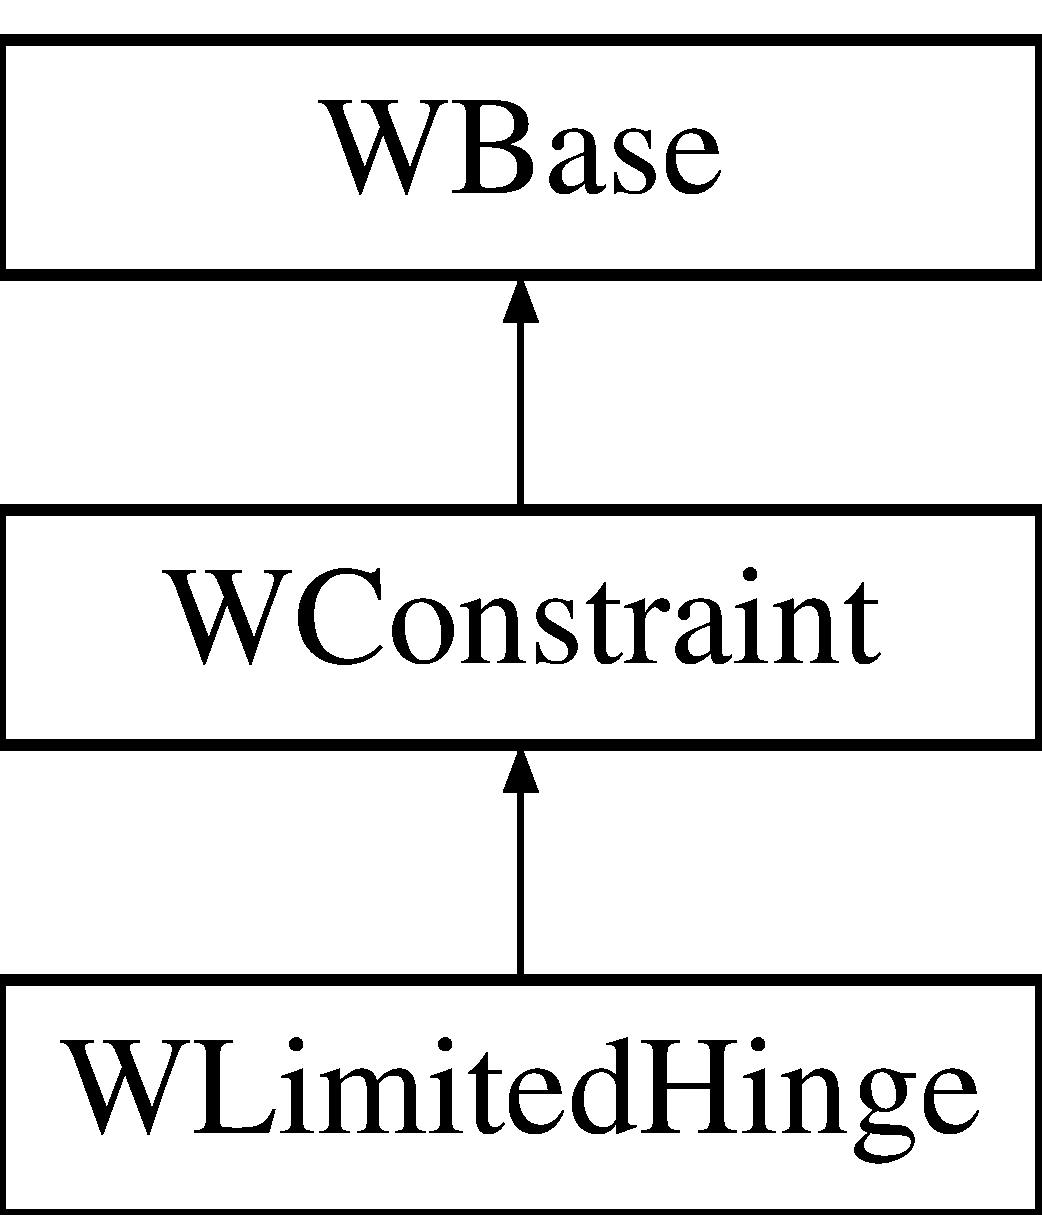
\includegraphics[height=3.000000cm]{class_w_limited_hinge}
\end{center}
\end{figure}
\subsection*{Public Member Functions}
\begin{DoxyCompactItemize}
\item 
{\bfseries W\+Limited\+Hinge} (class \hyperlink{class_wasabi}{Wasabi} $\ast$const app, unsigned int ID=0)\hypertarget{class_w_limited_hinge_afb877862b34866ea9c5eb752d0b5ac76}{}\label{class_w_limited_hinge_afb877862b34866ea9c5eb752d0b5ac76}

\item 
void {\bfseries Build} (const \hyperlink{class_w_rigid_body}{W\+Rigid\+Body} $\ast$const rb1, const \hyperlink{class_w_rigid_body}{W\+Rigid\+Body} $\ast$const rb2, bool breakable=false)\hypertarget{class_w_limited_hinge_a1459654753eb6d47c1b88f49598e4edd}{}\label{class_w_limited_hinge_a1459654753eb6d47c1b88f49598e4edd}

\item 
void {\bfseries Set\+Position\+World} (float x, float y, float z, float axisX, float axisY, float axisZ)\hypertarget{class_w_limited_hinge_a236904087d888f79a180456560c1fd1d}{}\label{class_w_limited_hinge_a236904087d888f79a180456560c1fd1d}

\item 
void {\bfseries Set\+Position\+World} (\hyperlink{class_w_vector3}{W\+Vector3} position, \hyperlink{class_w_vector3}{W\+Vector3} axis)\hypertarget{class_w_limited_hinge_a7281548f7929429985999207b10f2bf5}{}\label{class_w_limited_hinge_a7281548f7929429985999207b10f2bf5}

\item 
void {\bfseries Set\+Position\+Local} (float x1, float y1, float z1, float x2, float y2, float z2, float axis\+X1, float axis\+Y1, float axis\+Z1, float axis\+X2, float axis\+Y2, float axis\+Z2, float axis\+X1perp, float axis\+Y1perp, float axis\+Z1perp, float axis\+X2perp, float axis\+Y2perp, float axis\+Z2perp)\hypertarget{class_w_limited_hinge_ab99476cc864800f8cce746a31576296f}{}\label{class_w_limited_hinge_ab99476cc864800f8cce746a31576296f}

\item 
void {\bfseries Set\+Position\+Local} (\hyperlink{class_w_vector3}{W\+Vector3} position1, \hyperlink{class_w_vector3}{W\+Vector3} position2, \hyperlink{class_w_vector3}{W\+Vector3} axis1, \hyperlink{class_w_vector3}{W\+Vector3} axis2, \hyperlink{class_w_vector3}{W\+Vector3} axis1perp, \hyperlink{class_w_vector3}{W\+Vector3} axis2perp)\hypertarget{class_w_limited_hinge_a28c5c36b031cab8ce38c920ab73c04e3}{}\label{class_w_limited_hinge_a28c5c36b031cab8ce38c920ab73c04e3}

\item 
void {\bfseries Set\+Maximum\+Angle} (float angle)\hypertarget{class_w_limited_hinge_a46782450f40d6a23b24eb43ba095c912}{}\label{class_w_limited_hinge_a46782450f40d6a23b24eb43ba095c912}

\item 
void {\bfseries Set\+Minimum\+Angle} (float angle)\hypertarget{class_w_limited_hinge_a5259add02a20a4f8fa0f758cc7bf2e76}{}\label{class_w_limited_hinge_a5259add02a20a4f8fa0f758cc7bf2e76}

\item 
void {\bfseries Set\+Tau\+Factor} (float factor)\hypertarget{class_w_limited_hinge_a75d6917491789b4929828ed719f40f0f}{}\label{class_w_limited_hinge_a75d6917491789b4929828ed719f40f0f}

\item 
void {\bfseries Set\+Max\+Friction\+Torque} (float torque)\hypertarget{class_w_limited_hinge_aa304dee708fe9be400088d3f9acedbc2}{}\label{class_w_limited_hinge_aa304dee708fe9be400088d3f9acedbc2}

\item 
void {\bfseries Set\+Motor} (void(\+\_\+\+\_\+cdecl $\ast$cb)(const class hkp\+Callback\+Constraint\+Motor \&motor, const class hkp\+Constraint\+Motor\+Input $\ast$input, class hkp\+Constraint\+Motor\+Output $\ast$output), float f\+Min\+Force, float f\+Max\+Force)\hypertarget{class_w_limited_hinge_a4c05bb7a53ef80e5505afc613599eb81}{}\label{class_w_limited_hinge_a4c05bb7a53ef80e5505afc613599eb81}

\item 
void {\bfseries Enable\+Motor} ()\hypertarget{class_w_limited_hinge_af57eda17cf2afa143a2d9b65cafa13d2}{}\label{class_w_limited_hinge_af57eda17cf2afa143a2d9b65cafa13d2}

\item 
void {\bfseries Disable\+Motor} ()\hypertarget{class_w_limited_hinge_a0d72d1dd34ee5431e8c799d83a9d40fc}{}\label{class_w_limited_hinge_a0d72d1dd34ee5431e8c799d83a9d40fc}

\item 
void {\bfseries Set\+Motor\+Target\+Angle} (float ang)\hypertarget{class_w_limited_hinge_a28d71d70cd50bed09540a77e3f50cc29}{}\label{class_w_limited_hinge_a28d71d70cd50bed09540a77e3f50cc29}

\end{DoxyCompactItemize}
\subsection*{Protected Attributes}
\begin{DoxyCompactItemize}
\item 
hkp\+Limited\+Hinge\+Constraint\+Data $\ast$ {\bfseries m\+\_\+lhc}\hypertarget{class_w_limited_hinge_a6f25ed08c2f11e3146aee6ddada72695}{}\label{class_w_limited_hinge_a6f25ed08c2f11e3146aee6ddada72695}

\end{DoxyCompactItemize}


The documentation for this class was generated from the following file\+:\begin{DoxyCompactItemize}
\item 
Wasabi/\+Physics/\+Havok/W\+Havok\+Physics.\+h\end{DoxyCompactItemize}

\hypertarget{class_w_manager}{}\section{W\+Manager$<$ T $>$ Class Template Reference}
\label{class_w_manager}\index{W\+Manager$<$ T $>$@{W\+Manager$<$ T $>$}}


{\ttfamily \#include $<$W\+Manager.\+h$>$}

\subsection*{Public Member Functions}
\begin{DoxyCompactItemize}
\item 
{\bfseries W\+Manager} (class \hyperlink{class_wasabi}{Wasabi} $\ast$const a)\hypertarget{class_w_manager_a664b28788a3733ff3119a528b7938137}{}\label{class_w_manager_a664b28788a3733ff3119a528b7938137}

\item 
void \hyperlink{class_w_manager_a9261664705e037ebe5e9c3701cd076f8}{Add\+Entity} (T $\ast$entity)
\item 
bool \hyperlink{class_w_manager_ab8cf0a65733d5347aa33bed8bc7e31d0}{Remove\+Entity} (T $\ast$entity)
\item 
virtual void \hyperlink{class_w_manager_ae20a5e3888b58881c60d0edcc0b30ff6}{Init} ()
\item 
T $\ast$ \hyperlink{class_w_manager_a0b5bee24b16f3a5e68aa34b1b530e699}{Get\+Entity} (unsigned int ID) const 
\item 
T $\ast$ \hyperlink{class_w_manager_a3d60263193f1e86b141cd49674756faf}{Get\+Entity} (std\+::string name) const 
\item 
T $\ast$ \hyperlink{class_w_manager_a02635cc3416f475cb6be4ba1861c4f12}{Get\+Entity\+By\+Index} (unsigned int index) const 
\item 
unsigned int \hyperlink{class_w_manager_ade73debf402ea3a0a04b4dfdc0360a91}{Get\+Entities\+Count} (void) const 
\end{DoxyCompactItemize}
\subsection*{Public Attributes}
\begin{DoxyCompactItemize}
\item 
class \hyperlink{class_wasabi}{Wasabi} $\ast$const \hyperlink{class_w_manager_ac25fc4a5d0ae81526d34b67ac7067915}{m\+\_\+app}
\end{DoxyCompactItemize}
\subsection*{Protected Member Functions}
\begin{DoxyCompactItemize}
\item 
virtual std\+::string \hyperlink{class_w_manager_a85a6c2f77d8b477358b58948325e0298}{Get\+Type\+Name} () const  =0
\end{DoxyCompactItemize}
\subsection*{Protected Attributes}
\begin{DoxyCompactItemize}
\item 
std\+::vector$<$ T $\ast$ $>$ \hyperlink{class_w_manager_aad7041fe4813ac2bee7bb8380ed02b68}{m\+\_\+entities} \mbox{[}W\+\_\+\+H\+A\+S\+H\+T\+A\+B\+L\+E\+S\+I\+ZE\mbox{]}
\end{DoxyCompactItemize}


\subsection{Detailed Description}
\subsubsection*{template$<$typename T$>$\\*
class W\+Manager$<$ T $>$}

A \hyperlink{class_w_manager}{W\+Manager} is a template for a class that manages classes which inherit from a \hyperlink{class_w_base}{W\+Base}. A manager has a list of all instances of the class that it manages, as long as the class makes sure it registers itself (usually in its constructor) and removes itself upon destruction (usually in its destructor). 

\subsection{Member Function Documentation}
\index{W\+Manager@{W\+Manager}!Add\+Entity@{Add\+Entity}}
\index{Add\+Entity@{Add\+Entity}!W\+Manager@{W\+Manager}}
\subsubsection[{\texorpdfstring{Add\+Entity(\+T $\ast$entity)}{AddEntity(T *entity)}}]{\setlength{\rightskip}{0pt plus 5cm}template$<$typename T$>$ void {\bf W\+Manager}$<$ T $>$\+::Add\+Entity (
\begin{DoxyParamCaption}
\item[{T $\ast$}]{entity}
\end{DoxyParamCaption}
)\hspace{0.3cm}{\ttfamily [inline]}}\hypertarget{class_w_manager_a9261664705e037ebe5e9c3701cd076f8}{}\label{class_w_manager_a9261664705e037ebe5e9c3701cd076f8}
Registers an entity in the manager. 
\begin{DoxyParams}{Parameters}
{\em entity} & Pointer to the entity to register \\
\hline
\end{DoxyParams}
\index{W\+Manager@{W\+Manager}!Get\+Entities\+Count@{Get\+Entities\+Count}}
\index{Get\+Entities\+Count@{Get\+Entities\+Count}!W\+Manager@{W\+Manager}}
\subsubsection[{\texorpdfstring{Get\+Entities\+Count(void) const }{GetEntitiesCount(void) const }}]{\setlength{\rightskip}{0pt plus 5cm}template$<$typename T$>$ unsigned int {\bf W\+Manager}$<$ T $>$\+::Get\+Entities\+Count (
\begin{DoxyParamCaption}
\item[{void}]{}
\end{DoxyParamCaption}
) const\hspace{0.3cm}{\ttfamily [inline]}}\hypertarget{class_w_manager_ade73debf402ea3a0a04b4dfdc0360a91}{}\label{class_w_manager_ade73debf402ea3a0a04b4dfdc0360a91}
Retrieves the number of registered entities. \begin{DoxyReturn}{Returns}
Number of registered entities 
\end{DoxyReturn}
\index{W\+Manager@{W\+Manager}!Get\+Entity@{Get\+Entity}}
\index{Get\+Entity@{Get\+Entity}!W\+Manager@{W\+Manager}}
\subsubsection[{\texorpdfstring{Get\+Entity(unsigned int I\+D) const }{GetEntity(unsigned int ID) const }}]{\setlength{\rightskip}{0pt plus 5cm}template$<$typename T$>$ T$\ast$ {\bf W\+Manager}$<$ T $>$\+::Get\+Entity (
\begin{DoxyParamCaption}
\item[{unsigned int}]{ID}
\end{DoxyParamCaption}
) const\hspace{0.3cm}{\ttfamily [inline]}}\hypertarget{class_w_manager_a0b5bee24b16f3a5e68aa34b1b530e699}{}\label{class_w_manager_a0b5bee24b16f3a5e68aa34b1b530e699}
Retrieves a registered entity using its ID. 
\begin{DoxyParams}{Parameters}
{\em ID} & ID of the registered object \\
\hline
\end{DoxyParams}
\begin{DoxyReturn}{Returns}
The registered object, nullptr if its not found 
\end{DoxyReturn}
\index{W\+Manager@{W\+Manager}!Get\+Entity@{Get\+Entity}}
\index{Get\+Entity@{Get\+Entity}!W\+Manager@{W\+Manager}}
\subsubsection[{\texorpdfstring{Get\+Entity(std\+::string name) const }{GetEntity(std::string name) const }}]{\setlength{\rightskip}{0pt plus 5cm}template$<$typename T$>$ T$\ast$ {\bf W\+Manager}$<$ T $>$\+::Get\+Entity (
\begin{DoxyParamCaption}
\item[{std\+::string}]{name}
\end{DoxyParamCaption}
) const\hspace{0.3cm}{\ttfamily [inline]}}\hypertarget{class_w_manager_a3d60263193f1e86b141cd49674756faf}{}\label{class_w_manager_a3d60263193f1e86b141cd49674756faf}
Retrieves a registered entity using its name. 
\begin{DoxyParams}{Parameters}
{\em name} & Name of the object to retrieve \\
\hline
\end{DoxyParams}
\begin{DoxyReturn}{Returns}
The registered object, nullptr if its not found 
\end{DoxyReturn}
\index{W\+Manager@{W\+Manager}!Get\+Entity\+By\+Index@{Get\+Entity\+By\+Index}}
\index{Get\+Entity\+By\+Index@{Get\+Entity\+By\+Index}!W\+Manager@{W\+Manager}}
\subsubsection[{\texorpdfstring{Get\+Entity\+By\+Index(unsigned int index) const }{GetEntityByIndex(unsigned int index) const }}]{\setlength{\rightskip}{0pt plus 5cm}template$<$typename T$>$ T$\ast$ {\bf W\+Manager}$<$ T $>$\+::Get\+Entity\+By\+Index (
\begin{DoxyParamCaption}
\item[{unsigned int}]{index}
\end{DoxyParamCaption}
) const\hspace{0.3cm}{\ttfamily [inline]}}\hypertarget{class_w_manager_a02635cc3416f475cb6be4ba1861c4f12}{}\label{class_w_manager_a02635cc3416f475cb6be4ba1861c4f12}
Retrieves a registered entity using its index into the hashtable. 
\begin{DoxyParams}{Parameters}
{\em index} & Index of the object to retrieve \\
\hline
\end{DoxyParams}
\begin{DoxyReturn}{Returns}
The registered object, nullptr if its not found 
\end{DoxyReturn}
\index{W\+Manager@{W\+Manager}!Get\+Type\+Name@{Get\+Type\+Name}}
\index{Get\+Type\+Name@{Get\+Type\+Name}!W\+Manager@{W\+Manager}}
\subsubsection[{\texorpdfstring{Get\+Type\+Name() const  =0}{GetTypeName() const  =0}}]{\setlength{\rightskip}{0pt plus 5cm}template$<$typename T$>$ virtual std\+::string {\bf W\+Manager}$<$ T $>$\+::Get\+Type\+Name (
\begin{DoxyParamCaption}
{}
\end{DoxyParamCaption}
) const\hspace{0.3cm}{\ttfamily [protected]}, {\ttfamily [pure virtual]}}\hypertarget{class_w_manager_a85a6c2f77d8b477358b58948325e0298}{}\label{class_w_manager_a85a6c2f77d8b477358b58948325e0298}
This function must be implemented by a child class. It should return the name of the object that it is managing, which can be used for debugging purposes. \begin{DoxyReturn}{Returns}
\mbox{[}description\mbox{]} 
\end{DoxyReturn}
\index{W\+Manager@{W\+Manager}!Init@{Init}}
\index{Init@{Init}!W\+Manager@{W\+Manager}}
\subsubsection[{\texorpdfstring{Init()}{Init()}}]{\setlength{\rightskip}{0pt plus 5cm}template$<$typename T$>$ virtual void {\bf W\+Manager}$<$ T $>$\+::Init (
\begin{DoxyParamCaption}
{}
\end{DoxyParamCaption}
)\hspace{0.3cm}{\ttfamily [inline]}, {\ttfamily [virtual]}}\hypertarget{class_w_manager_ae20a5e3888b58881c60d0edcc0b30ff6}{}\label{class_w_manager_ae20a5e3888b58881c60d0edcc0b30ff6}
Initializes the manager. 

Reimplemented in \hyperlink{class_w_rigid_body_manager_a9b50ffc3505be62ab855e6b25cba2049}{W\+Rigid\+Body\+Manager}.

\index{W\+Manager@{W\+Manager}!Remove\+Entity@{Remove\+Entity}}
\index{Remove\+Entity@{Remove\+Entity}!W\+Manager@{W\+Manager}}
\subsubsection[{\texorpdfstring{Remove\+Entity(\+T $\ast$entity)}{RemoveEntity(T *entity)}}]{\setlength{\rightskip}{0pt plus 5cm}template$<$typename T$>$ bool {\bf W\+Manager}$<$ T $>$\+::Remove\+Entity (
\begin{DoxyParamCaption}
\item[{T $\ast$}]{entity}
\end{DoxyParamCaption}
)\hspace{0.3cm}{\ttfamily [inline]}}\hypertarget{class_w_manager_ab8cf0a65733d5347aa33bed8bc7e31d0}{}\label{class_w_manager_ab8cf0a65733d5347aa33bed8bc7e31d0}
De-\/registers an entity from the manager. 
\begin{DoxyParams}{Parameters}
{\em entity} & Entity to de-\/register \\
\hline
\end{DoxyParams}
\begin{DoxyReturn}{Returns}
true if the entity was found (and de-\/registered), false otherwise 
\end{DoxyReturn}


\subsection{Member Data Documentation}
\index{W\+Manager@{W\+Manager}!m\+\_\+app@{m\+\_\+app}}
\index{m\+\_\+app@{m\+\_\+app}!W\+Manager@{W\+Manager}}
\subsubsection[{\texorpdfstring{m\+\_\+app}{m_app}}]{\setlength{\rightskip}{0pt plus 5cm}template$<$typename T$>$ class {\bf Wasabi}$\ast$ const {\bf W\+Manager}$<$ T $>$\+::m\+\_\+app}\hypertarget{class_w_manager_ac25fc4a5d0ae81526d34b67ac7067915}{}\label{class_w_manager_ac25fc4a5d0ae81526d34b67ac7067915}
Pointer to the \hyperlink{class_wasabi}{Wasabi} instance that made this manager \index{W\+Manager@{W\+Manager}!m\+\_\+entities@{m\+\_\+entities}}
\index{m\+\_\+entities@{m\+\_\+entities}!W\+Manager@{W\+Manager}}
\subsubsection[{\texorpdfstring{m\+\_\+entities}{m_entities}}]{\setlength{\rightskip}{0pt plus 5cm}template$<$typename T$>$ std\+::vector$<$T$\ast$$>$ {\bf W\+Manager}$<$ T $>$\+::m\+\_\+entities\mbox{[}W\+\_\+\+H\+A\+S\+H\+T\+A\+B\+L\+E\+S\+I\+ZE\mbox{]}\hspace{0.3cm}{\ttfamily [protected]}}\hypertarget{class_w_manager_aad7041fe4813ac2bee7bb8380ed02b68}{}\label{class_w_manager_aad7041fe4813ac2bee7bb8380ed02b68}
a hash table of all entities registered 

The documentation for this class was generated from the following file\+:\begin{DoxyCompactItemize}
\item 
Wasabi/\+Core/W\+Manager.\+h\end{DoxyCompactItemize}

\hypertarget{class_w_marble_action}{}\section{W\+Marble\+Action Class Reference}
\label{class_w_marble_action}\index{W\+Marble\+Action@{W\+Marble\+Action}}
Inheritance diagram for W\+Marble\+Action\+:\begin{figure}[H]
\begin{center}
\leavevmode
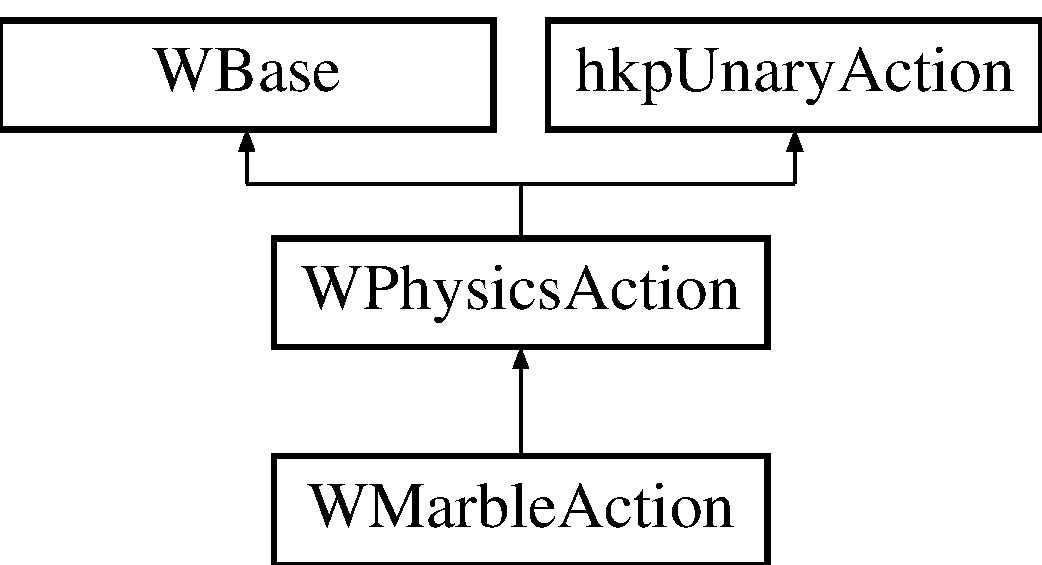
\includegraphics[height=3.000000cm]{class_w_marble_action}
\end{center}
\end{figure}
\subsection*{Public Member Functions}
\begin{DoxyCompactItemize}
\item 
{\bfseries W\+Marble\+Action} (class \hyperlink{class_wasabi}{Wasabi} $\ast$const app, \hyperlink{class_w_rigid_body}{W\+Rigid\+Body} $\ast$const body, unsigned int ID=0)\hypertarget{class_w_marble_action_a0c3da13df96d650bc49e72029a426f81}{}\label{class_w_marble_action_a0c3da13df96d650bc49e72029a426f81}

\item 
void {\bfseries apply\+Action} (const hk\+Step\+Info \&step\+Info)\hypertarget{class_w_marble_action_a38afd07ee30429279759ab7fd6f0c381}{}\label{class_w_marble_action_a38afd07ee30429279759ab7fd6f0c381}

\item 
void {\bfseries Set\+Forward\+Pressed} (bool pressed)\hypertarget{class_w_marble_action_a3e148ecb1505df538f9106e2d41a3656}{}\label{class_w_marble_action_a3e148ecb1505df538f9106e2d41a3656}

\item 
void {\bfseries Set\+Backward\+Pressed} (bool pressed)\hypertarget{class_w_marble_action_aa06bbbcc6bb19aa8cba3f04498085935}{}\label{class_w_marble_action_aa06bbbcc6bb19aa8cba3f04498085935}

\item 
void {\bfseries Set\+Turn\+Left\+Pressed} (bool pressed)\hypertarget{class_w_marble_action_a110d2dcad3a695aee54604a2abf2c3d2}{}\label{class_w_marble_action_a110d2dcad3a695aee54604a2abf2c3d2}

\item 
void {\bfseries Set\+Turn\+Right\+Pressed} (bool pressed)\hypertarget{class_w_marble_action_aa63d0d2a94fe8bfbad21e0854c1570f9}{}\label{class_w_marble_action_aa63d0d2a94fe8bfbad21e0854c1570f9}

\item 
void {\bfseries Set\+Jump\+Pressed} (bool pressed)\hypertarget{class_w_marble_action_a4ad398c66e8a6a53ac39de46e701cdb9}{}\label{class_w_marble_action_a4ad398c66e8a6a53ac39de46e701cdb9}

\item 
void {\bfseries Set\+Brake\+Pressed} (bool pressed)\hypertarget{class_w_marble_action_a6188a6f4c3dd1580eb338a237c6c3cb0}{}\label{class_w_marble_action_a6188a6f4c3dd1580eb338a237c6c3cb0}

\item 
void {\bfseries Set\+Stop\+Pressed} (bool pressed)\hypertarget{class_w_marble_action_aff88d139a0a4c1ae9a2b3ae708478538}{}\label{class_w_marble_action_aff88d139a0a4c1ae9a2b3ae708478538}

\item 
void {\bfseries Set\+Jumping\+Info} (float f\+Multiplier, float f\+Marble\+Radius)\hypertarget{class_w_marble_action_a14302384b7ccdf2da793c6fb55647397}{}\label{class_w_marble_action_a14302384b7ccdf2da793c6fb55647397}

\item 
void {\bfseries Set\+Rotation\+Info} (float f\+Multiplier)\hypertarget{class_w_marble_action_a292db2891d003dd872de64f526e96b20}{}\label{class_w_marble_action_a292db2891d003dd872de64f526e96b20}

\item 
void {\bfseries Set\+Acceleration\+Info} (float f\+Multiplier)\hypertarget{class_w_marble_action_aa1bc67c95dd103b65ce367a89fbafdde}{}\label{class_w_marble_action_aa1bc67c95dd103b65ce367a89fbafdde}

\item 
bool {\bfseries Is\+On\+Ground} () const \hypertarget{class_w_marble_action_ae6d3156c4890d0543ad85bea9ce0fb54}{}\label{class_w_marble_action_ae6d3156c4890d0543ad85bea9ce0fb54}

\item 
void {\bfseries Set\+Motion\+Direction} (\hyperlink{class_w_vector3}{W\+Vector3} dir)\hypertarget{class_w_marble_action_ab870f71fab4073ce01885dc1f2ed0995}{}\label{class_w_marble_action_ab870f71fab4073ce01885dc1f2ed0995}

\item 
\hyperlink{class_w_vector3}{W\+Vector3} {\bfseries Get\+Motion\+Direction} () const \hypertarget{class_w_marble_action_af563d9853a24040160b0177e57009849}{}\label{class_w_marble_action_af563d9853a24040160b0177e57009849}

\end{DoxyCompactItemize}
\subsection*{Protected Attributes}
\begin{DoxyCompactItemize}
\item 
float {\bfseries m\+\_\+impulse\+Scale}\hypertarget{class_w_marble_action_a1803e661066ddcfffcbc789c1f4c4a14}{}\label{class_w_marble_action_a1803e661066ddcfffcbc789c1f4c4a14}

\item 
float {\bfseries m\+\_\+rotation\+Increment}\hypertarget{class_w_marble_action_a0b554620001061161294d9155ed0a375}{}\label{class_w_marble_action_a0b554620001061161294d9155ed0a375}

\item 
float {\bfseries m\+\_\+current\+Angle}\hypertarget{class_w_marble_action_a6cf76e32556cad5f89e762d29b1f3ab3}{}\label{class_w_marble_action_a6cf76e32556cad5f89e762d29b1f3ab3}

\item 
const hk\+Vector4 {\bfseries m\+\_\+forward}\hypertarget{class_w_marble_action_ac9ba4cab7667f01486470ffe62bb0893}{}\label{class_w_marble_action_ac9ba4cab7667f01486470ffe62bb0893}

\item 
\hyperlink{class_w_vector3}{W\+Vector3} {\bfseries m\+\_\+cur\+Dir}\hypertarget{class_w_marble_action_af20f447462f634fdf06210d2b0a1f9d0}{}\label{class_w_marble_action_af20f447462f634fdf06210d2b0a1f9d0}

\item 
float {\bfseries m\+\_\+jump\+Mul}\hypertarget{class_w_marble_action_a8c7c709fc2b9ef4297f238419363235a}{}\label{class_w_marble_action_a8c7c709fc2b9ef4297f238419363235a}

\item 
float {\bfseries m\+\_\+f\+Radius}\hypertarget{class_w_marble_action_a88a2a90cdb265ccaf987936566f0a621}{}\label{class_w_marble_action_a88a2a90cdb265ccaf987936566f0a621}

\item 
bool {\bfseries m\+\_\+b\+Forward}\hypertarget{class_w_marble_action_a86e2c1804cbb9447ef4e55ba5846785e}{}\label{class_w_marble_action_a86e2c1804cbb9447ef4e55ba5846785e}

\item 
bool {\bfseries m\+\_\+b\+Backward}\hypertarget{class_w_marble_action_a6196b186f5af5adf2ec888dfe312fe0f}{}\label{class_w_marble_action_a6196b186f5af5adf2ec888dfe312fe0f}

\item 
bool {\bfseries m\+\_\+b\+Left}\hypertarget{class_w_marble_action_a521d0a5350b3fe19ed63fd21f052f600}{}\label{class_w_marble_action_a521d0a5350b3fe19ed63fd21f052f600}

\item 
bool {\bfseries m\+\_\+b\+Right}\hypertarget{class_w_marble_action_a8cfb2837a650a2a73b6df1a4bc4d3388}{}\label{class_w_marble_action_a8cfb2837a650a2a73b6df1a4bc4d3388}

\item 
bool {\bfseries m\+\_\+b\+Jump}\hypertarget{class_w_marble_action_a2f18111ceb724aa6b03f342afd910ff1}{}\label{class_w_marble_action_a2f18111ceb724aa6b03f342afd910ff1}

\item 
bool {\bfseries m\+\_\+b\+Brake}\hypertarget{class_w_marble_action_ac6efcccaad1340eca0823952605fd8b9}{}\label{class_w_marble_action_ac6efcccaad1340eca0823952605fd8b9}

\item 
bool {\bfseries m\+\_\+b\+Stop}\hypertarget{class_w_marble_action_a60343644fce80e6460f4f7d3be9306cb}{}\label{class_w_marble_action_a60343644fce80e6460f4f7d3be9306cb}

\item 
bool {\bfseries m\+\_\+b\+On\+Ground}\hypertarget{class_w_marble_action_ae12f429ef9f4210c624eda19c125c8e9}{}\label{class_w_marble_action_ae12f429ef9f4210c624eda19c125c8e9}

\end{DoxyCompactItemize}


The documentation for this class was generated from the following file\+:\begin{DoxyCompactItemize}
\item 
Wasabi/\+Physics/\+Havok/W\+Havok\+Physics.\+h\end{DoxyCompactItemize}

\hypertarget{class_w_material}{}\section{W\+Material Class Reference}
\label{class_w_material}\index{W\+Material@{W\+Material}}


{\ttfamily \#include $<$W\+Material.\+h$>$}

Inheritance diagram for W\+Material\+:\begin{figure}[H]
\begin{center}
\leavevmode
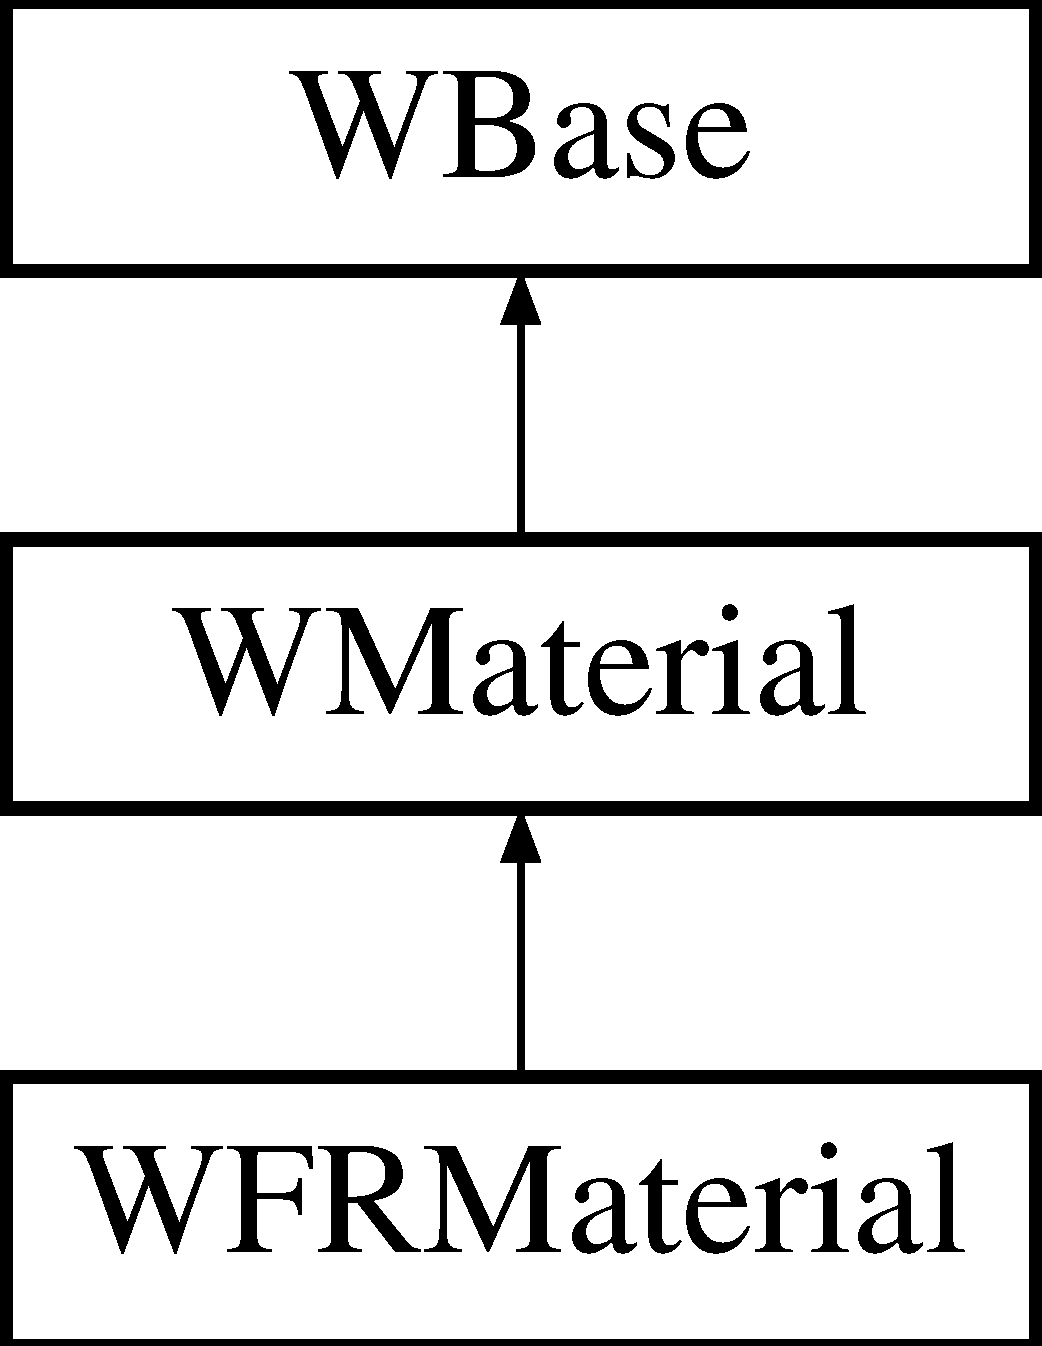
\includegraphics[height=3.000000cm]{class_w_material}
\end{center}
\end{figure}
\subsection*{Public Member Functions}
\begin{DoxyCompactItemize}
\item 
{\bfseries W\+Material} (class \hyperlink{class_wasabi}{Wasabi} $\ast$const app, unsigned int ID=0)\hypertarget{class_w_material_a5bfc9ab92d0ed404bd31e7e85a3a3306}{}\label{class_w_material_a5bfc9ab92d0ed404bd31e7e85a3a3306}

\item 
\hyperlink{class_w_error}{W\+Error} \hyperlink{class_w_material_ae48bfe0ea4d05867d077b8b48989c584}{Set\+Effect} (class \hyperlink{class_w_effect}{W\+Effect} $\ast$const effect)
\item 
virtual \hyperlink{class_w_error}{W\+Error} \hyperlink{class_w_material_a420e012110ddabf5410bab0805fac025}{Bind} (class \hyperlink{class_w_render_target}{W\+Render\+Target} $\ast$rt, unsigned int num\+\_\+vertex\+\_\+buffers=-\/1)
\item 
\hyperlink{class_w_error}{W\+Error} \hyperlink{class_w_material_ae2ec704f31b54ea0a1f8c9d30ea327d7}{Set\+Variable\+Float} (string var\+Name, float f\+Val)
\item 
\hyperlink{class_w_error}{W\+Error} \hyperlink{class_w_material_a28b095dc5ac19dc38dc8022bce985f91}{Set\+Variable\+Float\+Array} (string var\+Name, float $\ast$f\+Arr, int num\+\_\+elements)
\item 
\hyperlink{class_w_error}{W\+Error} \hyperlink{class_w_material_ac1fb138e3ef4b40fec3334e0ad569068}{Set\+Variable\+Int} (string var\+Name, int i\+Val)
\item 
\hyperlink{class_w_error}{W\+Error} \hyperlink{class_w_material_a1b0c5a02616ab0b8722c2c68e7e25c79}{Set\+Variable\+Int\+Array} (string var\+Name, int $\ast$i\+Arr, int num\+\_\+elements)
\item 
\hyperlink{class_w_error}{W\+Error} \hyperlink{class_w_material_aa791d00b4497df9ce81bab36df3fd369}{Set\+Variable\+Matrix} (string var\+Name, \hyperlink{class_w_matrix}{W\+Matrix} mtx)
\item 
\hyperlink{class_w_error}{W\+Error} \hyperlink{class_w_material_a4de2149658e89f97d79ced3e7ec18bcd}{Set\+Variable\+Vector2} (string var\+Name, \hyperlink{class_w_vector2}{W\+Vector2} vec)
\item 
\hyperlink{class_w_error}{W\+Error} \hyperlink{class_w_material_a09edc2496ed59ab067e3c8a412856d74}{Set\+Variable\+Vector3} (string var\+Name, \hyperlink{class_w_vector3}{W\+Vector3} vec)
\item 
\hyperlink{class_w_error}{W\+Error} \hyperlink{class_w_material_a8ea8adcd3f141f3896adc680e141d02b}{Set\+Variable\+Vector4} (string var\+Name, \hyperlink{class_w_vector4}{W\+Vector4} vec)
\item 
\hyperlink{class_w_error}{W\+Error} \hyperlink{class_w_material_a2d477cb8e3d6cf35a377b4fd438f01d0}{Set\+Variable\+Color} (string var\+Name, \hyperlink{class_w_color}{W\+Color} col)
\item 
\hyperlink{class_w_error}{W\+Error} \hyperlink{class_w_material_ab7a25be78f0609fce4e88bfdcd6aadcb}{Set\+Variable\+Data} (string var\+Name, void $\ast$data, int len)
\item 
\hyperlink{class_w_error}{W\+Error} \hyperlink{class_w_material_a4936e1d25fd3ecce6fbef960eeb75fdf}{Set\+Texture} (int binding\+\_\+index, class \hyperlink{class_w_image}{W\+Image} $\ast$img)
\item 
\hyperlink{class_w_error}{W\+Error} \hyperlink{class_w_material_a02d31133d0c88cd8def56318bb69ff90}{Set\+Animation\+Texture} (class \hyperlink{class_w_image}{W\+Image} $\ast$img)
\item 
\hyperlink{class_w_error}{W\+Error} \hyperlink{class_w_material_ac2ec1357e8a694111bb352711dbfe123}{Set\+Instancing\+Texture} (class \hyperlink{class_w_image}{W\+Image} $\ast$img)
\item 
class \hyperlink{class_w_effect}{W\+Effect} $\ast$ \hyperlink{class_w_material_af80d6b296601457db6d35283c3e3d206}{Get\+Effect} () const 
\item 
virtual bool \hyperlink{class_w_material_a73cd4716c62a5a331f32e211ebd54654}{Valid} () const 
\end{DoxyCompactItemize}
\subsection*{Additional Inherited Members}


\subsection{Detailed Description}
A \hyperlink{class_w_material}{W\+Material} contains the information needed to pass shader parameters to W\+Effects and their shaders. Parameters include all types of variables and textures. W\+Materials provide a convenient interface for setting values without having to deal with memory mapping between the host and the client (The R\+AM and the G\+PU memory). An effect (\hyperlink{class_w_effect}{W\+Effect}) cannot be used without a material, and thus object rendering requires a material (See \hyperlink{class_w_object_add4eb131afa0b55fbb4d5695eee7569c}{W\+Object\+::\+Set\+Material()}). 

\subsection{Member Function Documentation}
\index{W\+Material@{W\+Material}!Bind@{Bind}}
\index{Bind@{Bind}!W\+Material@{W\+Material}}
\subsubsection[{\texorpdfstring{Bind(class W\+Render\+Target $\ast$rt, unsigned int num\+\_\+vertex\+\_\+buffers=-\/1)}{Bind(class WRenderTarget *rt, unsigned int num_vertex_buffers=-1)}}]{\setlength{\rightskip}{0pt plus 5cm}{\bf W\+Error} W\+Material\+::\+Bind (
\begin{DoxyParamCaption}
\item[{class {\bf W\+Render\+Target} $\ast$}]{rt, }
\item[{unsigned int}]{num\+\_\+vertex\+\_\+buffers = {\ttfamily -\/1}}
\end{DoxyParamCaption}
)\hspace{0.3cm}{\ttfamily [virtual]}}\hypertarget{class_w_material_a420e012110ddabf5410bab0805fac025}{}\label{class_w_material_a420e012110ddabf5410bab0805fac025}
Binds the material and its effect to the graphics pipeline. A child class may choose to override this to change the binding procedure, or apply a certain operation upon binding. The render target must have its Begin() function called before this function is called. 
\begin{DoxyParams}{Parameters}
{\em rt} & Render target whose pipeline is being used \\
\hline
{\em num\+\_\+vertex\+\_\+buffers} & Number of vertex buffers that the material needs to render, valid values are either 0 if the effect uses no vertex buffers, or 1 to the number of input layouts in the effect \\
\hline
\end{DoxyParams}
\begin{DoxyReturn}{Returns}
Error code, see \hyperlink{_w_error_8h}{W\+Error.\+h} 
\end{DoxyReturn}


Reimplemented in \hyperlink{class_w_f_r_material_ab57a021a6e21d2c6dc872d6ea4450093}{W\+F\+R\+Material}.

\index{W\+Material@{W\+Material}!Get\+Effect@{Get\+Effect}}
\index{Get\+Effect@{Get\+Effect}!W\+Material@{W\+Material}}
\subsubsection[{\texorpdfstring{Get\+Effect() const }{GetEffect() const }}]{\setlength{\rightskip}{0pt plus 5cm}class {\bf W\+Effect} $\ast$ W\+Material\+::\+Get\+Effect (
\begin{DoxyParamCaption}
{}
\end{DoxyParamCaption}
) const}\hypertarget{class_w_material_af80d6b296601457db6d35283c3e3d206}{}\label{class_w_material_af80d6b296601457db6d35283c3e3d206}
Retrieves the bound effect. \begin{DoxyReturn}{Returns}
The bound effect 
\end{DoxyReturn}
\index{W\+Material@{W\+Material}!Set\+Animation\+Texture@{Set\+Animation\+Texture}}
\index{Set\+Animation\+Texture@{Set\+Animation\+Texture}!W\+Material@{W\+Material}}
\subsubsection[{\texorpdfstring{Set\+Animation\+Texture(class W\+Image $\ast$img)}{SetAnimationTexture(class WImage *img)}}]{\setlength{\rightskip}{0pt plus 5cm}{\bf W\+Error} W\+Material\+::\+Set\+Animation\+Texture (
\begin{DoxyParamCaption}
\item[{class {\bf W\+Image} $\ast$}]{img}
\end{DoxyParamCaption}
)}\hypertarget{class_w_material_a02d31133d0c88cd8def56318bb69ff90}{}\label{class_w_material_a02d31133d0c88cd8def56318bb69ff90}
Sets the texture that the effect marks as the animation texture, if it exists. 
\begin{DoxyParams}{Parameters}
{\em img} & The image to set the texture to, can be nullptr \\
\hline
\end{DoxyParams}
\begin{DoxyReturn}{Returns}
Error code, see \hyperlink{_w_error_8h}{W\+Error.\+h} 
\end{DoxyReturn}
\index{W\+Material@{W\+Material}!Set\+Effect@{Set\+Effect}}
\index{Set\+Effect@{Set\+Effect}!W\+Material@{W\+Material}}
\subsubsection[{\texorpdfstring{Set\+Effect(class W\+Effect $\ast$const effect)}{SetEffect(class WEffect *const effect)}}]{\setlength{\rightskip}{0pt plus 5cm}{\bf W\+Error} W\+Material\+::\+Set\+Effect (
\begin{DoxyParamCaption}
\item[{class {\bf W\+Effect} $\ast$const}]{effect}
\end{DoxyParamCaption}
)}\hypertarget{class_w_material_ae48bfe0ea4d05867d077b8b48989c584}{}\label{class_w_material_ae48bfe0ea4d05867d077b8b48989c584}
Sets the effect that this material will use. 
\begin{DoxyParams}{Parameters}
{\em effect} & Effect to use \\
\hline
\end{DoxyParams}
\begin{DoxyReturn}{Returns}
Error code, see \hyperlink{_w_error_8h}{W\+Error.\+h} 
\end{DoxyReturn}
\index{W\+Material@{W\+Material}!Set\+Instancing\+Texture@{Set\+Instancing\+Texture}}
\index{Set\+Instancing\+Texture@{Set\+Instancing\+Texture}!W\+Material@{W\+Material}}
\subsubsection[{\texorpdfstring{Set\+Instancing\+Texture(class W\+Image $\ast$img)}{SetInstancingTexture(class WImage *img)}}]{\setlength{\rightskip}{0pt plus 5cm}{\bf W\+Error} W\+Material\+::\+Set\+Instancing\+Texture (
\begin{DoxyParamCaption}
\item[{class {\bf W\+Image} $\ast$}]{img}
\end{DoxyParamCaption}
)}\hypertarget{class_w_material_ac2ec1357e8a694111bb352711dbfe123}{}\label{class_w_material_ac2ec1357e8a694111bb352711dbfe123}
Sets the texture that the effect marks as the instancing texture, if it exists. 
\begin{DoxyParams}{Parameters}
{\em img} & The image to set the texture to, can be nullptr \\
\hline
\end{DoxyParams}
\begin{DoxyReturn}{Returns}
Error code, see \hyperlink{_w_error_8h}{W\+Error.\+h} 
\end{DoxyReturn}
\index{W\+Material@{W\+Material}!Set\+Texture@{Set\+Texture}}
\index{Set\+Texture@{Set\+Texture}!W\+Material@{W\+Material}}
\subsubsection[{\texorpdfstring{Set\+Texture(int binding\+\_\+index, class W\+Image $\ast$img)}{SetTexture(int binding_index, class WImage *img)}}]{\setlength{\rightskip}{0pt plus 5cm}{\bf W\+Error} W\+Material\+::\+Set\+Texture (
\begin{DoxyParamCaption}
\item[{int}]{binding\+\_\+index, }
\item[{class {\bf W\+Image} $\ast$}]{img}
\end{DoxyParamCaption}
)}\hypertarget{class_w_material_a4936e1d25fd3ecce6fbef960eeb75fdf}{}\label{class_w_material_a4936e1d25fd3ecce6fbef960eeb75fdf}
Sets a texture in the bound effect. 
\begin{DoxyParams}{Parameters}
{\em binding\+\_\+index} & The binding index of the texture \\
\hline
{\em img} & The image to set the texture to, can be nullptr \\
\hline
\end{DoxyParams}
\begin{DoxyReturn}{Returns}
Error code, see \hyperlink{_w_error_8h}{W\+Error.\+h} 
\end{DoxyReturn}
\index{W\+Material@{W\+Material}!Set\+Variable\+Color@{Set\+Variable\+Color}}
\index{Set\+Variable\+Color@{Set\+Variable\+Color}!W\+Material@{W\+Material}}
\subsubsection[{\texorpdfstring{Set\+Variable\+Color(string var\+Name, W\+Color col)}{SetVariableColor(string varName, WColor col)}}]{\setlength{\rightskip}{0pt plus 5cm}{\bf W\+Error} W\+Material\+::\+Set\+Variable\+Color (
\begin{DoxyParamCaption}
\item[{string}]{var\+Name, }
\item[{{\bf W\+Color}}]{col}
\end{DoxyParamCaption}
)}\hypertarget{class_w_material_a2d477cb8e3d6cf35a377b4fd438f01d0}{}\label{class_w_material_a2d477cb8e3d6cf35a377b4fd438f01d0}
Sets a variable in one of the bound effect\textquotesingle{}s shaders whose name is var\+Name and whose type is a color. If multiple variables have the same name, they will all be set. 
\begin{DoxyParams}{Parameters}
{\em var\+Name} & Name of the variable to set \\
\hline
{\em col} & Value to set \\
\hline
\end{DoxyParams}
\begin{DoxyReturn}{Returns}
Error code, see \hyperlink{_w_error_8h}{W\+Error.\+h} 
\end{DoxyReturn}
\index{W\+Material@{W\+Material}!Set\+Variable\+Data@{Set\+Variable\+Data}}
\index{Set\+Variable\+Data@{Set\+Variable\+Data}!W\+Material@{W\+Material}}
\subsubsection[{\texorpdfstring{Set\+Variable\+Data(string var\+Name, void $\ast$data, int len)}{SetVariableData(string varName, void *data, int len)}}]{\setlength{\rightskip}{0pt plus 5cm}{\bf W\+Error} W\+Material\+::\+Set\+Variable\+Data (
\begin{DoxyParamCaption}
\item[{string}]{var\+Name, }
\item[{void $\ast$}]{data, }
\item[{int}]{len}
\end{DoxyParamCaption}
)}\hypertarget{class_w_material_ab7a25be78f0609fce4e88bfdcd6aadcb}{}\label{class_w_material_ab7a25be78f0609fce4e88bfdcd6aadcb}
Sets a variable in one of the bound effect\textquotesingle{}s shaders whose name is var\+Name and whose type can be anything. The set variable\textquotesingle{}s size must match the len parameter for successful setting. If multiple variables have the same name, they will all be set. 
\begin{DoxyParams}{Parameters}
{\em var\+Name} & Name of the variable to set \\
\hline
{\em data} & Address of the memory to set the variable\textquotesingle{}s data to \\
\hline
{\em len} & Length of data, in bytes \\
\hline
\end{DoxyParams}
\begin{DoxyReturn}{Returns}
Error code, see \hyperlink{_w_error_8h}{W\+Error.\+h} 
\end{DoxyReturn}
\index{W\+Material@{W\+Material}!Set\+Variable\+Float@{Set\+Variable\+Float}}
\index{Set\+Variable\+Float@{Set\+Variable\+Float}!W\+Material@{W\+Material}}
\subsubsection[{\texorpdfstring{Set\+Variable\+Float(string var\+Name, float f\+Val)}{SetVariableFloat(string varName, float fVal)}}]{\setlength{\rightskip}{0pt plus 5cm}{\bf W\+Error} W\+Material\+::\+Set\+Variable\+Float (
\begin{DoxyParamCaption}
\item[{string}]{var\+Name, }
\item[{float}]{f\+Val}
\end{DoxyParamCaption}
)}\hypertarget{class_w_material_ae2ec704f31b54ea0a1f8c9d30ea327d7}{}\label{class_w_material_ae2ec704f31b54ea0a1f8c9d30ea327d7}
Sets a variable in one of the bound effect\textquotesingle{}s shaders whose name is var\+Name and whose type is a float. If multiple variables have the same name, they will all be set. 
\begin{DoxyParams}{Parameters}
{\em var\+Name} & Name of the variable to set \\
\hline
{\em f\+Val} & Value to set \\
\hline
\end{DoxyParams}
\begin{DoxyReturn}{Returns}
Error code, see \hyperlink{_w_error_8h}{W\+Error.\+h} 
\end{DoxyReturn}
\index{W\+Material@{W\+Material}!Set\+Variable\+Float\+Array@{Set\+Variable\+Float\+Array}}
\index{Set\+Variable\+Float\+Array@{Set\+Variable\+Float\+Array}!W\+Material@{W\+Material}}
\subsubsection[{\texorpdfstring{Set\+Variable\+Float\+Array(string var\+Name, float $\ast$f\+Arr, int num\+\_\+elements)}{SetVariableFloatArray(string varName, float *fArr, int num_elements)}}]{\setlength{\rightskip}{0pt plus 5cm}{\bf W\+Error} W\+Material\+::\+Set\+Variable\+Float\+Array (
\begin{DoxyParamCaption}
\item[{string}]{var\+Name, }
\item[{float $\ast$}]{f\+Arr, }
\item[{int}]{num\+\_\+elements}
\end{DoxyParamCaption}
)}\hypertarget{class_w_material_a28b095dc5ac19dc38dc8022bce985f91}{}\label{class_w_material_a28b095dc5ac19dc38dc8022bce985f91}
Sets a variable in one of the bound effect\textquotesingle{}s shaders whose name is var\+Name and whose type is an array of floats. If multiple variables have the same name, they will all be set. 
\begin{DoxyParams}{Parameters}
{\em var\+Name} & Name of the variable to set \\
\hline
{\em f\+Arr} & Address of the array to set \\
\hline
{\em num\+\_\+elements} & Number of elements in f\+Arr \\
\hline
\end{DoxyParams}
\begin{DoxyReturn}{Returns}
Error code, see \hyperlink{_w_error_8h}{W\+Error.\+h} 
\end{DoxyReturn}
\index{W\+Material@{W\+Material}!Set\+Variable\+Int@{Set\+Variable\+Int}}
\index{Set\+Variable\+Int@{Set\+Variable\+Int}!W\+Material@{W\+Material}}
\subsubsection[{\texorpdfstring{Set\+Variable\+Int(string var\+Name, int i\+Val)}{SetVariableInt(string varName, int iVal)}}]{\setlength{\rightskip}{0pt plus 5cm}{\bf W\+Error} W\+Material\+::\+Set\+Variable\+Int (
\begin{DoxyParamCaption}
\item[{string}]{var\+Name, }
\item[{int}]{i\+Val}
\end{DoxyParamCaption}
)}\hypertarget{class_w_material_ac1fb138e3ef4b40fec3334e0ad569068}{}\label{class_w_material_ac1fb138e3ef4b40fec3334e0ad569068}
Sets a variable in one of the bound effect\textquotesingle{}s shaders whose name is var\+Name and whose type is an integer. If multiple variables have the same name, they will all be set. 
\begin{DoxyParams}{Parameters}
{\em var\+Name} & Name of the variable to set \\
\hline
{\em i\+Val} & Value to set \\
\hline
\end{DoxyParams}
\begin{DoxyReturn}{Returns}
Error code, see \hyperlink{_w_error_8h}{W\+Error.\+h} 
\end{DoxyReturn}
\index{W\+Material@{W\+Material}!Set\+Variable\+Int\+Array@{Set\+Variable\+Int\+Array}}
\index{Set\+Variable\+Int\+Array@{Set\+Variable\+Int\+Array}!W\+Material@{W\+Material}}
\subsubsection[{\texorpdfstring{Set\+Variable\+Int\+Array(string var\+Name, int $\ast$i\+Arr, int num\+\_\+elements)}{SetVariableIntArray(string varName, int *iArr, int num_elements)}}]{\setlength{\rightskip}{0pt plus 5cm}{\bf W\+Error} W\+Material\+::\+Set\+Variable\+Int\+Array (
\begin{DoxyParamCaption}
\item[{string}]{var\+Name, }
\item[{int $\ast$}]{i\+Arr, }
\item[{int}]{num\+\_\+elements}
\end{DoxyParamCaption}
)}\hypertarget{class_w_material_a1b0c5a02616ab0b8722c2c68e7e25c79}{}\label{class_w_material_a1b0c5a02616ab0b8722c2c68e7e25c79}
Sets a variable in one of the bound effect\textquotesingle{}s shaders whose name is var\+Name and whose type is an array of integers. If multiple variables have the same name, they will all be set. 
\begin{DoxyParams}{Parameters}
{\em var\+Name} & Name of the variable to set \\
\hline
{\em i\+Arr} & Address of the array to set \\
\hline
{\em num\+\_\+elements} & Number of elements in f\+Arr \\
\hline
\end{DoxyParams}
\begin{DoxyReturn}{Returns}
Error code, see \hyperlink{_w_error_8h}{W\+Error.\+h} 
\end{DoxyReturn}
\index{W\+Material@{W\+Material}!Set\+Variable\+Matrix@{Set\+Variable\+Matrix}}
\index{Set\+Variable\+Matrix@{Set\+Variable\+Matrix}!W\+Material@{W\+Material}}
\subsubsection[{\texorpdfstring{Set\+Variable\+Matrix(string var\+Name, W\+Matrix mtx)}{SetVariableMatrix(string varName, WMatrix mtx)}}]{\setlength{\rightskip}{0pt plus 5cm}{\bf W\+Error} W\+Material\+::\+Set\+Variable\+Matrix (
\begin{DoxyParamCaption}
\item[{string}]{var\+Name, }
\item[{{\bf W\+Matrix}}]{mtx}
\end{DoxyParamCaption}
)}\hypertarget{class_w_material_aa791d00b4497df9ce81bab36df3fd369}{}\label{class_w_material_aa791d00b4497df9ce81bab36df3fd369}
Sets a variable in one of the bound effect\textquotesingle{}s shaders whose name is var\+Name and whose type is a matrix. If multiple variables have the same name, they will all be set. 
\begin{DoxyParams}{Parameters}
{\em var\+Name} & Name of the variable to set \\
\hline
{\em mtx} & Value to set \\
\hline
\end{DoxyParams}
\begin{DoxyReturn}{Returns}
Error code, see \hyperlink{_w_error_8h}{W\+Error.\+h} 
\end{DoxyReturn}
\index{W\+Material@{W\+Material}!Set\+Variable\+Vector2@{Set\+Variable\+Vector2}}
\index{Set\+Variable\+Vector2@{Set\+Variable\+Vector2}!W\+Material@{W\+Material}}
\subsubsection[{\texorpdfstring{Set\+Variable\+Vector2(string var\+Name, W\+Vector2 vec)}{SetVariableVector2(string varName, WVector2 vec)}}]{\setlength{\rightskip}{0pt plus 5cm}{\bf W\+Error} W\+Material\+::\+Set\+Variable\+Vector2 (
\begin{DoxyParamCaption}
\item[{string}]{var\+Name, }
\item[{{\bf W\+Vector2}}]{vec}
\end{DoxyParamCaption}
)}\hypertarget{class_w_material_a4de2149658e89f97d79ced3e7ec18bcd}{}\label{class_w_material_a4de2149658e89f97d79ced3e7ec18bcd}
Sets a variable in one of the bound effect\textquotesingle{}s shaders whose name is var\+Name and whose type is a 2D vector. If multiple variables have the same name, they will all be set. 
\begin{DoxyParams}{Parameters}
{\em var\+Name} & Name of the variable to set \\
\hline
{\em vec} & Value to set \\
\hline
\end{DoxyParams}
\begin{DoxyReturn}{Returns}
Error code, see \hyperlink{_w_error_8h}{W\+Error.\+h} 
\end{DoxyReturn}
\index{W\+Material@{W\+Material}!Set\+Variable\+Vector3@{Set\+Variable\+Vector3}}
\index{Set\+Variable\+Vector3@{Set\+Variable\+Vector3}!W\+Material@{W\+Material}}
\subsubsection[{\texorpdfstring{Set\+Variable\+Vector3(string var\+Name, W\+Vector3 vec)}{SetVariableVector3(string varName, WVector3 vec)}}]{\setlength{\rightskip}{0pt plus 5cm}{\bf W\+Error} W\+Material\+::\+Set\+Variable\+Vector3 (
\begin{DoxyParamCaption}
\item[{string}]{var\+Name, }
\item[{{\bf W\+Vector3}}]{vec}
\end{DoxyParamCaption}
)}\hypertarget{class_w_material_a09edc2496ed59ab067e3c8a412856d74}{}\label{class_w_material_a09edc2496ed59ab067e3c8a412856d74}
Sets a variable in one of the bound effect\textquotesingle{}s shaders whose name is var\+Name and whose type is a 3D vector. If multiple variables have the same name, they will all be set. 
\begin{DoxyParams}{Parameters}
{\em var\+Name} & Name of the variable to set \\
\hline
{\em vec} & Value to set \\
\hline
\end{DoxyParams}
\begin{DoxyReturn}{Returns}
Error code, see \hyperlink{_w_error_8h}{W\+Error.\+h} 
\end{DoxyReturn}
\index{W\+Material@{W\+Material}!Set\+Variable\+Vector4@{Set\+Variable\+Vector4}}
\index{Set\+Variable\+Vector4@{Set\+Variable\+Vector4}!W\+Material@{W\+Material}}
\subsubsection[{\texorpdfstring{Set\+Variable\+Vector4(string var\+Name, W\+Vector4 vec)}{SetVariableVector4(string varName, WVector4 vec)}}]{\setlength{\rightskip}{0pt plus 5cm}{\bf W\+Error} W\+Material\+::\+Set\+Variable\+Vector4 (
\begin{DoxyParamCaption}
\item[{string}]{var\+Name, }
\item[{{\bf W\+Vector4}}]{vec}
\end{DoxyParamCaption}
)}\hypertarget{class_w_material_a8ea8adcd3f141f3896adc680e141d02b}{}\label{class_w_material_a8ea8adcd3f141f3896adc680e141d02b}
Sets a variable in one of the bound effect\textquotesingle{}s shaders whose name is var\+Name and whose type is a 4D vector. If multiple variables have the same name, they will all be set. 
\begin{DoxyParams}{Parameters}
{\em var\+Name} & Name of the variable to set \\
\hline
{\em vec} & Value to set \\
\hline
\end{DoxyParams}
\begin{DoxyReturn}{Returns}
Error code, see \hyperlink{_w_error_8h}{W\+Error.\+h} 
\end{DoxyReturn}
\index{W\+Material@{W\+Material}!Valid@{Valid}}
\index{Valid@{Valid}!W\+Material@{W\+Material}}
\subsubsection[{\texorpdfstring{Valid() const }{Valid() const }}]{\setlength{\rightskip}{0pt plus 5cm}bool W\+Material\+::\+Valid (
\begin{DoxyParamCaption}
\item[{void}]{}
\end{DoxyParamCaption}
) const\hspace{0.3cm}{\ttfamily [virtual]}}\hypertarget{class_w_material_a73cd4716c62a5a331f32e211ebd54654}{}\label{class_w_material_a73cd4716c62a5a331f32e211ebd54654}
Checks the validity of the material. A material is valid if it has a valid effect assigned to it. \begin{DoxyReturn}{Returns}
true of the material is valid, false otherwise 
\end{DoxyReturn}


Implements \hyperlink{class_w_base_a76ac973ba9a43e182f6a6a4869d69725}{W\+Base}.



The documentation for this class was generated from the following files\+:\begin{DoxyCompactItemize}
\item 
Wasabi/\+Materials/W\+Material.\+h\item 
Wasabi/\+Materials/W\+Material.\+cpp\end{DoxyCompactItemize}

\hypertarget{class_w_material_manager}{}\section{W\+Material\+Manager Class Reference}
\label{class_w_material_manager}\index{W\+Material\+Manager@{W\+Material\+Manager}}


{\ttfamily \#include $<$W\+Material.\+h$>$}

Inheritance diagram for W\+Material\+Manager\+:\begin{figure}[H]
\begin{center}
\leavevmode
\includegraphics[height=2.000000cm]{class_w_material_manager}
\end{center}
\end{figure}
\subsection*{Public Member Functions}
\begin{DoxyCompactItemize}
\item 
{\bfseries W\+Material\+Manager} (class \hyperlink{class_wasabi}{Wasabi} $\ast$const app)\hypertarget{class_w_material_manager_a0fd1d6202eadb0619c2790374f78d22c}{}\label{class_w_material_manager_a0fd1d6202eadb0619c2790374f78d22c}

\end{DoxyCompactItemize}
\subsection*{Friends}
\begin{DoxyCompactItemize}
\item 
class {\bfseries W\+Material}\hypertarget{class_w_material_manager_a82829be2ace0f839dd132dface8a4da3}{}\label{class_w_material_manager_a82829be2ace0f839dd132dface8a4da3}

\end{DoxyCompactItemize}
\subsection*{Additional Inherited Members}


\subsection{Detailed Description}
Manager class for \hyperlink{class_w_material}{W\+Material}. 

The documentation for this class was generated from the following files\+:\begin{DoxyCompactItemize}
\item 
Wasabi/\+Materials/W\+Material.\+h\item 
Wasabi/\+Materials/W\+Material.\+cpp\end{DoxyCompactItemize}

\hypertarget{class_w_matrix}{}\section{W\+Matrix Class Reference}
\label{class_w_matrix}\index{W\+Matrix@{W\+Matrix}}


{\ttfamily \#include $<$W\+Math.\+h$>$}

\subsection*{Public Member Functions}
\begin{DoxyCompactItemize}
\item 
{\bfseries W\+Matrix} (float f11, float f12, float f13, float f14, float f21, float f22, float f23, float f24, float f31, float f32, float f33, float f34, float f41, float f42, float f43, float f44)\hypertarget{class_w_matrix_aa626cd0267ca4e98fbf9672091613146}{}\label{class_w_matrix_aa626cd0267ca4e98fbf9672091613146}

\item 
{\bfseries operator float $\ast$} ()\hypertarget{class_w_matrix_a47199ab3ac019f3fba3f02369f2c3748}{}\label{class_w_matrix_a47199ab3ac019f3fba3f02369f2c3748}

\item 
{\bfseries operator const float $\ast$} ()\hypertarget{class_w_matrix_aa2aa5bec5b3684a351d92a3ec847be09}{}\label{class_w_matrix_aa2aa5bec5b3684a351d92a3ec847be09}

\item 
const \hyperlink{class_w_matrix}{W\+Matrix} {\bfseries operator+} (const \hyperlink{class_w_matrix}{W\+Matrix} m) const \hypertarget{class_w_matrix_a4c54b602a9a8d5df9e7967516da9fe37}{}\label{class_w_matrix_a4c54b602a9a8d5df9e7967516da9fe37}

\item 
const \hyperlink{class_w_matrix}{W\+Matrix} {\bfseries operator-\/} (const \hyperlink{class_w_matrix}{W\+Matrix} m) const \hypertarget{class_w_matrix_aa3cff5673c4904d75eb3c4224773be8f}{}\label{class_w_matrix_aa3cff5673c4904d75eb3c4224773be8f}

\item 
const \hyperlink{class_w_matrix}{W\+Matrix} {\bfseries operator$\ast$} (const \hyperlink{class_w_matrix}{W\+Matrix} m) const \hypertarget{class_w_matrix_ac974d1a20acec0e6759f34091521b47f}{}\label{class_w_matrix_ac974d1a20acec0e6759f34091521b47f}

\item 
const \hyperlink{class_w_matrix}{W\+Matrix} {\bfseries operator/} (const \hyperlink{class_w_matrix}{W\+Matrix} m) const \hypertarget{class_w_matrix_aee12db71d36897e441457066d5f17a8e}{}\label{class_w_matrix_aee12db71d36897e441457066d5f17a8e}

\item 
const \hyperlink{class_w_matrix}{W\+Matrix} {\bfseries operator$\ast$} (const float f) const \hypertarget{class_w_matrix_a0c6d2cb720b0e7620ba863d1e184263c}{}\label{class_w_matrix_a0c6d2cb720b0e7620ba863d1e184263c}

\item 
const \hyperlink{class_w_matrix}{W\+Matrix} {\bfseries operator/} (const float f) const \hypertarget{class_w_matrix_ac0376add51280792d8664b98f3fcd462}{}\label{class_w_matrix_ac0376add51280792d8664b98f3fcd462}

\item 
void {\bfseries operator+=} (const \hyperlink{class_w_matrix}{W\+Matrix} m)\hypertarget{class_w_matrix_ad80488df1025a940932467d40898bccc}{}\label{class_w_matrix_ad80488df1025a940932467d40898bccc}

\item 
void {\bfseries operator-\/=} (const \hyperlink{class_w_matrix}{W\+Matrix} m)\hypertarget{class_w_matrix_add6710e3f502f42d270878f1f7cbff5e}{}\label{class_w_matrix_add6710e3f502f42d270878f1f7cbff5e}

\item 
void {\bfseries operator$\ast$=} (const \hyperlink{class_w_matrix}{W\+Matrix} m)\hypertarget{class_w_matrix_a884beb6a0fd099568cff7b1f9c893295}{}\label{class_w_matrix_a884beb6a0fd099568cff7b1f9c893295}

\item 
void {\bfseries operator/=} (const \hyperlink{class_w_matrix}{W\+Matrix} m)\hypertarget{class_w_matrix_a44f8f2a7973364cca98b735371f73f65}{}\label{class_w_matrix_a44f8f2a7973364cca98b735371f73f65}

\item 
void {\bfseries operator$\ast$=} (const float f)\hypertarget{class_w_matrix_a30a1c2c062e2069dc864bd896773cee0}{}\label{class_w_matrix_a30a1c2c062e2069dc864bd896773cee0}

\item 
void {\bfseries operator/=} (const float f)\hypertarget{class_w_matrix_af19ffc53b742e21bd831f1831a74ec06}{}\label{class_w_matrix_af19ffc53b742e21bd831f1831a74ec06}

\item 
float \& {\bfseries operator()} (const unsigned int row, const unsigned int col)\hypertarget{class_w_matrix_a926c3ded2ce466784fcc1cb7482b8d2e}{}\label{class_w_matrix_a926c3ded2ce466784fcc1cb7482b8d2e}

\item 
const float {\bfseries operator()} (const unsigned int row, const unsigned int col) const \hypertarget{class_w_matrix_acb2e3b174261fdbe0fdf5f5cdd255e42}{}\label{class_w_matrix_acb2e3b174261fdbe0fdf5f5cdd255e42}

\item 
float \& {\bfseries operator\mbox{[}$\,$\mbox{]}} (const unsigned int index)\hypertarget{class_w_matrix_a72f442646a5078dca447b411c98358ea}{}\label{class_w_matrix_a72f442646a5078dca447b411c98358ea}

\item 
const float {\bfseries operator\mbox{[}$\,$\mbox{]}} (const unsigned int index) const \hypertarget{class_w_matrix_ae4feef61fae0a9c253820e0201425d57}{}\label{class_w_matrix_ae4feef61fae0a9c253820e0201425d57}

\end{DoxyCompactItemize}
\subsection*{Public Attributes}
\begin{DoxyCompactItemize}
\item 
float \hyperlink{class_w_matrix_a3103a31e4270d2a0997fa895dcfe3e52}{mat} \mbox{[}16\mbox{]}
\end{DoxyCompactItemize}


\subsection{Detailed Description}
A 4D matrix. 

\subsection{Member Data Documentation}
\index{W\+Matrix@{W\+Matrix}!mat@{mat}}
\index{mat@{mat}!W\+Matrix@{W\+Matrix}}
\subsubsection[{\texorpdfstring{mat}{mat}}]{\setlength{\rightskip}{0pt plus 5cm}float W\+Matrix\+::mat\mbox{[}16\mbox{]}}\hypertarget{class_w_matrix_a3103a31e4270d2a0997fa895dcfe3e52}{}\label{class_w_matrix_a3103a31e4270d2a0997fa895dcfe3e52}
Matrix components (row-\/major) 

The documentation for this class was generated from the following files\+:\begin{DoxyCompactItemize}
\item 
Wasabi/\+Core/W\+Math.\+h\item 
Wasabi/\+Core/W\+Math.\+cpp\end{DoxyCompactItemize}

\hypertarget{class_w_object}{}\section{W\+Object Class Reference}
\label{class_w_object}\index{W\+Object@{W\+Object}}


{\ttfamily \#include $<$W\+Object.\+h$>$}

Inheritance diagram for W\+Object\+:\begin{figure}[H]
\begin{center}
\leavevmode
\includegraphics[height=2.000000cm]{class_w_object}
\end{center}
\end{figure}
\subsection*{Public Member Functions}
\begin{DoxyCompactItemize}
\item 
{\bfseries W\+Object} (\hyperlink{class_wasabi}{Wasabi} $\ast$const app, unsigned int ID=0)\hypertarget{class_w_object_ae01d22761e4282b9f3d3ebf23d64f4b8}{}\label{class_w_object_ae01d22761e4282b9f3d3ebf23d64f4b8}

\item 
void \hyperlink{class_w_object_a315a4d624c6e6c5fef996e1dd87abe33}{Render} (class \hyperlink{class_w_render_target}{W\+Render\+Target} $\ast$rt)
\item 
\hyperlink{class_w_error}{W\+Error} \hyperlink{class_w_object_a473a8002f7bb6581ecb38937ff1df10e}{Set\+Geometry} (class \hyperlink{class_w_geometry}{W\+Geometry} $\ast$geometry)
\item 
\hyperlink{class_w_error}{W\+Error} \hyperlink{class_w_object_add4eb131afa0b55fbb4d5695eee7569c}{Set\+Material} (class \hyperlink{class_w_material}{W\+Material} $\ast$material)
\item 
\hyperlink{class_w_error}{W\+Error} \hyperlink{class_w_object_aa78d1b389d67bc5a9ee9fd64d559e64a}{Set\+Animation} (class \hyperlink{class_w_animation}{W\+Animation} $\ast$animation)
\item 
class \hyperlink{class_w_geometry}{W\+Geometry} $\ast$ \hyperlink{class_w_object_a21ff26282c4c6e76b9e93749a53e8a67}{Get\+Geometry} () const 
\item 
class \hyperlink{class_w_material}{W\+Material} $\ast$ \hyperlink{class_w_object_a4832d77d13177c26165833be034db5b3}{Get\+Material} () const 
\item 
class \hyperlink{class_w_animation}{W\+Animation} $\ast$ \hyperlink{class_w_object_a1fd40c0623b666c46a5d5a4508dec979}{Get\+Animation} () const 
\item 
\hyperlink{class_w_error}{W\+Error} \hyperlink{class_w_object_a3eb6c8b80c1cc3ca3149be1647f3abb4}{Init\+Instancing} (unsigned int max\+Instances)
\item 
\hyperlink{class_w_instance}{W\+Instance} $\ast$ \hyperlink{class_w_object_acb0daac5850075a54b012703bab0b589}{Create\+Instance} ()
\item 
\hyperlink{class_w_instance}{W\+Instance} $\ast$ \hyperlink{class_w_object_a144ebe9b2effa5355d3e5c243d871ced}{Get\+Instance} (unsigned int index) const 
\item 
void \hyperlink{class_w_object_ad408d0bc44bbcc7deabfd979caad3edd}{Delete\+Instance} (\hyperlink{class_w_instance}{W\+Instance} $\ast$instance)
\item 
void \hyperlink{class_w_object_a8f7264e7168585f60d82f6183fa35e5e}{Delete\+Instance} (unsigned int index)
\item 
unsigned int \hyperlink{class_w_object_a05dea54bb2a586ac92c51c260f542041}{Get\+Instances\+Count} () const 
\item 
void \hyperlink{class_w_object_a2f1ca8ef071fb6c259502555d6b5a47c}{Show} ()
\item 
void \hyperlink{class_w_object_a72a9f879a85cf26d72548ffc8835ad67}{Hide} ()
\item 
bool \hyperlink{class_w_object_a83f2fef49f037cac8a26f966174ecdcc}{Hidden} () const 
\item 
void \hyperlink{class_w_object_a50ad933e853950919c8742bf12bc90e8}{Enable\+Frustum\+Culling} ()
\item 
void \hyperlink{class_w_object_a15a2fef8f1ebf38e8aeee70eabbf79b8}{Disable\+Frustum\+Culling} ()
\item 
void \hyperlink{class_w_object_a1dcebfccb9dda3a0eb0f08594834eca7}{Scale} (float x, float y, float z)
\item 
void \hyperlink{class_w_object_ad4632595db1f1f661e0abb0d72e452b0}{Scale} (\hyperlink{class_w_vector3}{W\+Vector3} scale)
\item 
void \hyperlink{class_w_object_a53bf6f7cadd2ffe1b59cf1231305f31c}{ScaleX} (float scale)
\item 
void \hyperlink{class_w_object_a12dde8e7596a2ce595c509abe86606bd}{ScaleY} (float scale)
\item 
void \hyperlink{class_w_object_a9b63d725ee1feb40dcc4facafdcb63fc}{ScaleZ} (float scale)
\item 
\hyperlink{class_w_vector3}{W\+Vector3} \hyperlink{class_w_object_a1229c3548ecc1b1b64c48afaee85c5ad}{Get\+Scale} () const 
\item 
float \hyperlink{class_w_object_ade99923c893f2daf6d650e15a09f527b}{Get\+ScaleX} () const 
\item 
float \hyperlink{class_w_object_a9954b5dca076b1af9348e60c15310931}{Get\+ScaleY} () const 
\item 
float \hyperlink{class_w_object_a7e9c4970b7af1731370c7de335ff1c9d}{Get\+ScaleZ} () const 
\item 
\hyperlink{class_w_matrix}{W\+Matrix} \hyperlink{class_w_object_a95a5b7ec4028d109ee8aef1c53334d15}{Get\+World\+Matrix} ()
\item 
bool \hyperlink{class_w_object_a5fa9d24d946c66ebd96d5291aaf1a273}{Update\+Locals} (\hyperlink{class_w_vector3}{W\+Vector3} offset=\hyperlink{class_w_vector3}{W\+Vector3}(0, 0, 0))
\item 
virtual void \hyperlink{class_w_object_a0e939f965dea9e524014c0dfc771d30f}{On\+State\+Change} (\hyperlink{_w_orientation_8h_afe94de0a48bbd7b343ab18bc318cef28}{S\+T\+A\+T\+E\+\_\+\+C\+H\+A\+N\+G\+E\+\_\+\+T\+Y\+PE} type)
\item 
virtual bool \hyperlink{class_w_object_a99b053864c7797f538f15728fc7f8a2c}{Valid} () const 
\end{DoxyCompactItemize}
\subsection*{Additional Inherited Members}


\subsection{Detailed Description}
A \hyperlink{class_w_object}{W\+Object} provides an easy way to render things in \hyperlink{class_wasabi}{Wasabi}. A \hyperlink{class_w_object}{W\+Object} combines \hyperlink{class_w_geometry}{W\+Geometry} and \hyperlink{class_w_material}{W\+Material} to render geometry using the material. Furthermore, \hyperlink{class_w_object}{W\+Object} provides an interface to manipulate the rendered object\textquotesingle{}s desired position, orientation and scale. A \hyperlink{class_w_object}{W\+Object} also provides an easy way to apply animations and instancing on rendered geometry. 

\subsection{Member Function Documentation}
\index{W\+Object@{W\+Object}!Create\+Instance@{Create\+Instance}}
\index{Create\+Instance@{Create\+Instance}!W\+Object@{W\+Object}}
\subsubsection[{\texorpdfstring{Create\+Instance()}{CreateInstance()}}]{\setlength{\rightskip}{0pt plus 5cm}{\bf W\+Instance} $\ast$ W\+Object\+::\+Create\+Instance (
\begin{DoxyParamCaption}
{}
\end{DoxyParamCaption}
)}\hypertarget{class_w_object_acb0daac5850075a54b012703bab0b589}{}\label{class_w_object_acb0daac5850075a54b012703bab0b589}
Creates an instance of this object. Instancing has to be initialized prior to calling this function (see \hyperlink{class_w_object_a3eb6c8b80c1cc3ca3149be1647f3abb4}{Init\+Instancing()}). \begin{DoxyReturn}{Returns}
The newly created instance, or nullptr if it cannot be created. An instance creation failure will occur if instancing is not initiated or if the maximum number of instances is reached 
\end{DoxyReturn}
\index{W\+Object@{W\+Object}!Delete\+Instance@{Delete\+Instance}}
\index{Delete\+Instance@{Delete\+Instance}!W\+Object@{W\+Object}}
\subsubsection[{\texorpdfstring{Delete\+Instance(\+W\+Instance $\ast$instance)}{DeleteInstance(WInstance *instance)}}]{\setlength{\rightskip}{0pt plus 5cm}void W\+Object\+::\+Delete\+Instance (
\begin{DoxyParamCaption}
\item[{{\bf W\+Instance} $\ast$}]{instance}
\end{DoxyParamCaption}
)}\hypertarget{class_w_object_ad408d0bc44bbcc7deabfd979caad3edd}{}\label{class_w_object_ad408d0bc44bbcc7deabfd979caad3edd}
Destroys an instance created for this object. The memory of the instance will be freed and {\bfseries The pointer given to the function cannot be used after this call}. 
\begin{DoxyParams}{Parameters}
{\em instance} & Instance to destroy \\
\hline
\end{DoxyParams}
\index{W\+Object@{W\+Object}!Delete\+Instance@{Delete\+Instance}}
\index{Delete\+Instance@{Delete\+Instance}!W\+Object@{W\+Object}}
\subsubsection[{\texorpdfstring{Delete\+Instance(unsigned int index)}{DeleteInstance(unsigned int index)}}]{\setlength{\rightskip}{0pt plus 5cm}void W\+Object\+::\+Delete\+Instance (
\begin{DoxyParamCaption}
\item[{unsigned int}]{index}
\end{DoxyParamCaption}
)}\hypertarget{class_w_object_a8f7264e7168585f60d82f6183fa35e5e}{}\label{class_w_object_a8f7264e7168585f60d82f6183fa35e5e}
Destroys an instance created for this object. {\bfseries Any pointer to the instance destroyed by this call cannot be used as that memory will be freed}. 
\begin{DoxyParams}{Parameters}
{\em index} & Index of the instance to destroy \\
\hline
\end{DoxyParams}
\index{W\+Object@{W\+Object}!Disable\+Frustum\+Culling@{Disable\+Frustum\+Culling}}
\index{Disable\+Frustum\+Culling@{Disable\+Frustum\+Culling}!W\+Object@{W\+Object}}
\subsubsection[{\texorpdfstring{Disable\+Frustum\+Culling()}{DisableFrustumCulling()}}]{\setlength{\rightskip}{0pt plus 5cm}void W\+Object\+::\+Disable\+Frustum\+Culling (
\begin{DoxyParamCaption}
{}
\end{DoxyParamCaption}
)}\hypertarget{class_w_object_a15a2fef8f1ebf38e8aeee70eabbf79b8}{}\label{class_w_object_a15a2fef8f1ebf38e8aeee70eabbf79b8}
Disables frustum culling, see \hyperlink{class_w_object_a50ad933e853950919c8742bf12bc90e8}{Enable\+Frustum\+Culling()} for more info. \index{W\+Object@{W\+Object}!Enable\+Frustum\+Culling@{Enable\+Frustum\+Culling}}
\index{Enable\+Frustum\+Culling@{Enable\+Frustum\+Culling}!W\+Object@{W\+Object}}
\subsubsection[{\texorpdfstring{Enable\+Frustum\+Culling()}{EnableFrustumCulling()}}]{\setlength{\rightskip}{0pt plus 5cm}void W\+Object\+::\+Enable\+Frustum\+Culling (
\begin{DoxyParamCaption}
{}
\end{DoxyParamCaption}
)}\hypertarget{class_w_object_a50ad933e853950919c8742bf12bc90e8}{}\label{class_w_object_a50ad933e853950919c8742bf12bc90e8}
Enables frustum culling. Frustum culling causes the object to only be rendered if part of its geometry is within the viewing frustum of the camera. \index{W\+Object@{W\+Object}!Get\+Animation@{Get\+Animation}}
\index{Get\+Animation@{Get\+Animation}!W\+Object@{W\+Object}}
\subsubsection[{\texorpdfstring{Get\+Animation() const }{GetAnimation() const }}]{\setlength{\rightskip}{0pt plus 5cm}{\bf W\+Animation} $\ast$ W\+Object\+::\+Get\+Animation (
\begin{DoxyParamCaption}
{}
\end{DoxyParamCaption}
) const}\hypertarget{class_w_object_a1fd40c0623b666c46a5d5a4508dec979}{}\label{class_w_object_a1fd40c0623b666c46a5d5a4508dec979}
Retrieves the attached animation. \begin{DoxyReturn}{Returns}
Attached animation, nullptr if none exists 
\end{DoxyReturn}
\index{W\+Object@{W\+Object}!Get\+Geometry@{Get\+Geometry}}
\index{Get\+Geometry@{Get\+Geometry}!W\+Object@{W\+Object}}
\subsubsection[{\texorpdfstring{Get\+Geometry() const }{GetGeometry() const }}]{\setlength{\rightskip}{0pt plus 5cm}{\bf W\+Geometry} $\ast$ W\+Object\+::\+Get\+Geometry (
\begin{DoxyParamCaption}
{}
\end{DoxyParamCaption}
) const}\hypertarget{class_w_object_a21ff26282c4c6e76b9e93749a53e8a67}{}\label{class_w_object_a21ff26282c4c6e76b9e93749a53e8a67}
Retrieves the attached geometry. \begin{DoxyReturn}{Returns}
Attached geometry, nullptr if none exists 
\end{DoxyReturn}
\index{W\+Object@{W\+Object}!Get\+Instance@{Get\+Instance}}
\index{Get\+Instance@{Get\+Instance}!W\+Object@{W\+Object}}
\subsubsection[{\texorpdfstring{Get\+Instance(unsigned int index) const }{GetInstance(unsigned int index) const }}]{\setlength{\rightskip}{0pt plus 5cm}{\bf W\+Instance} $\ast$ W\+Object\+::\+Get\+Instance (
\begin{DoxyParamCaption}
\item[{unsigned int}]{index}
\end{DoxyParamCaption}
) const}\hypertarget{class_w_object_a144ebe9b2effa5355d3e5c243d871ced}{}\label{class_w_object_a144ebe9b2effa5355d3e5c243d871ced}
Retrieves an instance of the object at a given index. 
\begin{DoxyParams}{Parameters}
{\em index} & Index of the instance to retrieve \\
\hline
\end{DoxyParams}
\begin{DoxyReturn}{Returns}
Pointer to the instance at the given index, or nullptr if it cannot be found 
\end{DoxyReturn}
\index{W\+Object@{W\+Object}!Get\+Instances\+Count@{Get\+Instances\+Count}}
\index{Get\+Instances\+Count@{Get\+Instances\+Count}!W\+Object@{W\+Object}}
\subsubsection[{\texorpdfstring{Get\+Instances\+Count() const }{GetInstancesCount() const }}]{\setlength{\rightskip}{0pt plus 5cm}unsigned int W\+Object\+::\+Get\+Instances\+Count (
\begin{DoxyParamCaption}
{}
\end{DoxyParamCaption}
) const}\hypertarget{class_w_object_a05dea54bb2a586ac92c51c260f542041}{}\label{class_w_object_a05dea54bb2a586ac92c51c260f542041}
Retrieves the number of instances for this object that are currently created. \begin{DoxyReturn}{Returns}
Number of currently created instances of the object 
\end{DoxyReturn}
\index{W\+Object@{W\+Object}!Get\+Material@{Get\+Material}}
\index{Get\+Material@{Get\+Material}!W\+Object@{W\+Object}}
\subsubsection[{\texorpdfstring{Get\+Material() const }{GetMaterial() const }}]{\setlength{\rightskip}{0pt plus 5cm}{\bf W\+Material} $\ast$ W\+Object\+::\+Get\+Material (
\begin{DoxyParamCaption}
{}
\end{DoxyParamCaption}
) const}\hypertarget{class_w_object_a4832d77d13177c26165833be034db5b3}{}\label{class_w_object_a4832d77d13177c26165833be034db5b3}
Retrieves the attached material. \begin{DoxyReturn}{Returns}
Attached material, nullptr if none exists 
\end{DoxyReturn}
\index{W\+Object@{W\+Object}!Get\+Scale@{Get\+Scale}}
\index{Get\+Scale@{Get\+Scale}!W\+Object@{W\+Object}}
\subsubsection[{\texorpdfstring{Get\+Scale() const }{GetScale() const }}]{\setlength{\rightskip}{0pt plus 5cm}{\bf W\+Vector3} W\+Object\+::\+Get\+Scale (
\begin{DoxyParamCaption}
{}
\end{DoxyParamCaption}
) const}\hypertarget{class_w_object_a1229c3548ecc1b1b64c48afaee85c5ad}{}\label{class_w_object_a1229c3548ecc1b1b64c48afaee85c5ad}
Retrieves the scale factors of this object. \begin{DoxyReturn}{Returns}
3D vector containing the scale factors 
\end{DoxyReturn}
\index{W\+Object@{W\+Object}!Get\+ScaleX@{Get\+ScaleX}}
\index{Get\+ScaleX@{Get\+ScaleX}!W\+Object@{W\+Object}}
\subsubsection[{\texorpdfstring{Get\+Scale\+X() const }{GetScaleX() const }}]{\setlength{\rightskip}{0pt plus 5cm}float W\+Object\+::\+Get\+ScaleX (
\begin{DoxyParamCaption}
{}
\end{DoxyParamCaption}
) const}\hypertarget{class_w_object_ade99923c893f2daf6d650e15a09f527b}{}\label{class_w_object_ade99923c893f2daf6d650e15a09f527b}
Retrieves the X scale of this object. \begin{DoxyReturn}{Returns}
Scale factor 
\end{DoxyReturn}
\index{W\+Object@{W\+Object}!Get\+ScaleY@{Get\+ScaleY}}
\index{Get\+ScaleY@{Get\+ScaleY}!W\+Object@{W\+Object}}
\subsubsection[{\texorpdfstring{Get\+Scale\+Y() const }{GetScaleY() const }}]{\setlength{\rightskip}{0pt plus 5cm}float W\+Object\+::\+Get\+ScaleY (
\begin{DoxyParamCaption}
{}
\end{DoxyParamCaption}
) const}\hypertarget{class_w_object_a9954b5dca076b1af9348e60c15310931}{}\label{class_w_object_a9954b5dca076b1af9348e60c15310931}
Retrieves the Y scale of this object. \begin{DoxyReturn}{Returns}
Scale factor 
\end{DoxyReturn}
\index{W\+Object@{W\+Object}!Get\+ScaleZ@{Get\+ScaleZ}}
\index{Get\+ScaleZ@{Get\+ScaleZ}!W\+Object@{W\+Object}}
\subsubsection[{\texorpdfstring{Get\+Scale\+Z() const }{GetScaleZ() const }}]{\setlength{\rightskip}{0pt plus 5cm}float W\+Object\+::\+Get\+ScaleZ (
\begin{DoxyParamCaption}
{}
\end{DoxyParamCaption}
) const}\hypertarget{class_w_object_a7e9c4970b7af1731370c7de335ff1c9d}{}\label{class_w_object_a7e9c4970b7af1731370c7de335ff1c9d}
Retrieves the Z scale of this object. \begin{DoxyReturn}{Returns}
Scale factor 
\end{DoxyReturn}
\index{W\+Object@{W\+Object}!Get\+World\+Matrix@{Get\+World\+Matrix}}
\index{Get\+World\+Matrix@{Get\+World\+Matrix}!W\+Object@{W\+Object}}
\subsubsection[{\texorpdfstring{Get\+World\+Matrix()}{GetWorldMatrix()}}]{\setlength{\rightskip}{0pt plus 5cm}{\bf W\+Matrix} W\+Object\+::\+Get\+World\+Matrix (
\begin{DoxyParamCaption}
{}
\end{DoxyParamCaption}
)}\hypertarget{class_w_object_a95a5b7ec4028d109ee8aef1c53334d15}{}\label{class_w_object_a95a5b7ec4028d109ee8aef1c53334d15}
Retrieves the world matrix computed so far. A call to \hyperlink{class_w_object_a5fa9d24d946c66ebd96d5291aaf1a273}{Update\+Locals()} should be made prior to this one to ensure getting the most recent matrix. \begin{DoxyReturn}{Returns}
World matrix of this object 
\end{DoxyReturn}
\index{W\+Object@{W\+Object}!Hidden@{Hidden}}
\index{Hidden@{Hidden}!W\+Object@{W\+Object}}
\subsubsection[{\texorpdfstring{Hidden() const }{Hidden() const }}]{\setlength{\rightskip}{0pt plus 5cm}bool W\+Object\+::\+Hidden (
\begin{DoxyParamCaption}
{}
\end{DoxyParamCaption}
) const}\hypertarget{class_w_object_a83f2fef49f037cac8a26f966174ecdcc}{}\label{class_w_object_a83f2fef49f037cac8a26f966174ecdcc}
Checks if the object is hidden. \begin{DoxyReturn}{Returns}
true if the object is hidden, false otherwise 
\end{DoxyReturn}
\index{W\+Object@{W\+Object}!Hide@{Hide}}
\index{Hide@{Hide}!W\+Object@{W\+Object}}
\subsubsection[{\texorpdfstring{Hide()}{Hide()}}]{\setlength{\rightskip}{0pt plus 5cm}void W\+Object\+::\+Hide (
\begin{DoxyParamCaption}
{}
\end{DoxyParamCaption}
)}\hypertarget{class_w_object_a72a9f879a85cf26d72548ffc8835ad67}{}\label{class_w_object_a72a9f879a85cf26d72548ffc8835ad67}
Hides the object, making it unable to render. \index{W\+Object@{W\+Object}!Init\+Instancing@{Init\+Instancing}}
\index{Init\+Instancing@{Init\+Instancing}!W\+Object@{W\+Object}}
\subsubsection[{\texorpdfstring{Init\+Instancing(unsigned int max\+Instances)}{InitInstancing(unsigned int maxInstances)}}]{\setlength{\rightskip}{0pt plus 5cm}{\bf W\+Error} W\+Object\+::\+Init\+Instancing (
\begin{DoxyParamCaption}
\item[{unsigned int}]{max\+Instances}
\end{DoxyParamCaption}
)}\hypertarget{class_w_object_a3eb6c8b80c1cc3ca3149be1647f3abb4}{}\label{class_w_object_a3eb6c8b80c1cc3ca3149be1647f3abb4}
Initiates geometry instancing for this object. When geometry instancing is initiated, and at least one instance is created (via \hyperlink{class_w_object_acb0daac5850075a54b012703bab0b589}{Create\+Instance()}), the object will be rendered with geometry instancing. 
\begin{DoxyParams}{Parameters}
{\em max\+Instances} & Maximum number of instanced allowed to be created \\
\hline
\end{DoxyParams}
\begin{DoxyReturn}{Returns}
Error code, see \hyperlink{_w_error_8h}{W\+Error.\+h} 
\end{DoxyReturn}
\index{W\+Object@{W\+Object}!On\+State\+Change@{On\+State\+Change}}
\index{On\+State\+Change@{On\+State\+Change}!W\+Object@{W\+Object}}
\subsubsection[{\texorpdfstring{On\+State\+Change(\+S\+T\+A\+T\+E\+\_\+\+C\+H\+A\+N\+G\+E\+\_\+\+T\+Y\+P\+E type)}{OnStateChange(STATE_CHANGE_TYPE type)}}]{\setlength{\rightskip}{0pt plus 5cm}void W\+Object\+::\+On\+State\+Change (
\begin{DoxyParamCaption}
\item[{{\bf S\+T\+A\+T\+E\+\_\+\+C\+H\+A\+N\+G\+E\+\_\+\+T\+Y\+PE}}]{type}
\end{DoxyParamCaption}
)\hspace{0.3cm}{\ttfamily [virtual]}}\hypertarget{class_w_object_a0e939f965dea9e524014c0dfc771d30f}{}\label{class_w_object_a0e939f965dea9e524014c0dfc771d30f}
A callback called by this class when the entity changes its position or orientation. 
\begin{DoxyParams}{Parameters}
{\em type} & Orientation change type \\
\hline
\end{DoxyParams}


Reimplemented from \hyperlink{class_w_orientation_aa765b7dcd772bbcc511c2c9317e7693c}{W\+Orientation}.

\index{W\+Object@{W\+Object}!Render@{Render}}
\index{Render@{Render}!W\+Object@{W\+Object}}
\subsubsection[{\texorpdfstring{Render(class W\+Render\+Target $\ast$rt)}{Render(class WRenderTarget *rt)}}]{\setlength{\rightskip}{0pt plus 5cm}void W\+Object\+::\+Render (
\begin{DoxyParamCaption}
\item[{class {\bf W\+Render\+Target} $\ast$}]{rt}
\end{DoxyParamCaption}
)}\hypertarget{class_w_object_a315a4d624c6e6c5fef996e1dd87abe33}{}\label{class_w_object_a315a4d624c6e6c5fef996e1dd87abe33}
Renders this object. An object will only render to the render target if its valid (see \hyperlink{class_w_object_a99b053864c7797f538f15728fc7f8a2c}{Valid()}) and not hidden (see \hyperlink{class_w_object_a72a9f879a85cf26d72548ffc8835ad67}{Hide()}). If frustum culling is enabled (see \hyperlink{class_w_object_a50ad933e853950919c8742bf12bc90e8}{Enable\+Frustum\+Culling()}), the object will only render if it is within the viewing frustum of the render target\textquotesingle{}s camera. Before an object binds its attached material (\hyperlink{class_w_material_a420e012110ddabf5410bab0805fac025}{W\+Material\+::\+Bind()}), it will set the following variables and resources in the material, if they exist\+:
\begin{DoxyItemize}
\item \char`\"{}g\+World\char`\"{} (\hyperlink{class_w_matrix}{W\+Matrix}) will be set to the world matrix of this object.
\item \char`\"{}g\+Projection\char`\"{} (\hyperlink{class_w_matrix}{W\+Matrix}) will be set to the projection matrix of the camera.
\item \char`\"{}g\+View\char`\"{} (\hyperlink{class_w_matrix}{W\+Matrix}) will be set to the view matrix of the camera.
\item \char`\"{}g\+Cam\+Pos\char`\"{} (\hyperlink{class_w_vector3}{W\+Vector3}) will be set to the world position of the camera.
\item \char`\"{}g\+Animation\char`\"{} (int) will be set to 1 if animation data is provided, 0 otherwise.
\item \char`\"{}g\+Instancing\char`\"{} (int) will be set to 1 if instancing data is provided, 0 otherwise.
\item \char`\"{}g\+Animation\+Texture\+Width\char`\"{} (int) will be set to the width of the animation texture. This will only be set if g\+Animation was set to 1.
\item \char`\"{}g\+Instance\+Texture\+Width\char`\"{} (int) will be set to the width of the instancing texture. This will only be set if g\+Instancing was set to 1.
\item \hyperlink{class_w_material_a02d31133d0c88cd8def56318bb69ff90}{W\+Material\+::\+Set\+Animation\+Texture()} will be called and assigned the animation texture from the attached animation. This will only occur if g\+Animation was set to 1.
\item \hyperlink{class_w_material_ac2ec1357e8a694111bb352711dbfe123}{W\+Material\+::\+Set\+Instancing\+Texture()} will be called and assigned the instancing texture created by this object. This will only occur if g\+Instancing was set to 1.
\end{DoxyItemize}

If the object\textquotesingle{}s instancing is initiated (see \hyperlink{class_w_object_a3eb6c8b80c1cc3ca3149be1647f3abb4}{Init\+Instancing()}), and there is at least one instance created (see \hyperlink{class_w_object_acb0daac5850075a54b012703bab0b589}{Create\+Instance()}), the object will be rendered using geometry instancing.


\begin{DoxyParams}{Parameters}
{\em rt} & Render target to render to. \\
\hline
\end{DoxyParams}
\index{W\+Object@{W\+Object}!Scale@{Scale}}
\index{Scale@{Scale}!W\+Object@{W\+Object}}
\subsubsection[{\texorpdfstring{Scale(float x, float y, float z)}{Scale(float x, float y, float z)}}]{\setlength{\rightskip}{0pt plus 5cm}void W\+Object\+::\+Scale (
\begin{DoxyParamCaption}
\item[{float}]{x, }
\item[{float}]{y, }
\item[{float}]{z}
\end{DoxyParamCaption}
)}\hypertarget{class_w_object_a1dcebfccb9dda3a0eb0f08594834eca7}{}\label{class_w_object_a1dcebfccb9dda3a0eb0f08594834eca7}
Sets the scale of this object. 
\begin{DoxyParams}{Parameters}
{\em x} & X scale multiplier \\
\hline
{\em y} & Y scale multiplier \\
\hline
{\em z} & Z scale multiplier \\
\hline
\end{DoxyParams}
\index{W\+Object@{W\+Object}!Scale@{Scale}}
\index{Scale@{Scale}!W\+Object@{W\+Object}}
\subsubsection[{\texorpdfstring{Scale(\+W\+Vector3 scale)}{Scale(WVector3 scale)}}]{\setlength{\rightskip}{0pt plus 5cm}void W\+Object\+::\+Scale (
\begin{DoxyParamCaption}
\item[{{\bf W\+Vector3}}]{scale}
\end{DoxyParamCaption}
)}\hypertarget{class_w_object_ad4632595db1f1f661e0abb0d72e452b0}{}\label{class_w_object_ad4632595db1f1f661e0abb0d72e452b0}
Sets the scale of this object. 
\begin{DoxyParams}{Parameters}
{\em scale} & Scale factor components \\
\hline
\end{DoxyParams}
\index{W\+Object@{W\+Object}!ScaleX@{ScaleX}}
\index{ScaleX@{ScaleX}!W\+Object@{W\+Object}}
\subsubsection[{\texorpdfstring{Scale\+X(float scale)}{ScaleX(float scale)}}]{\setlength{\rightskip}{0pt plus 5cm}void W\+Object\+::\+ScaleX (
\begin{DoxyParamCaption}
\item[{float}]{scale}
\end{DoxyParamCaption}
)}\hypertarget{class_w_object_a53bf6f7cadd2ffe1b59cf1231305f31c}{}\label{class_w_object_a53bf6f7cadd2ffe1b59cf1231305f31c}
Sets the X scale of this object. 
\begin{DoxyParams}{Parameters}
{\em scale} & Scale factor \\
\hline
\end{DoxyParams}
\index{W\+Object@{W\+Object}!ScaleY@{ScaleY}}
\index{ScaleY@{ScaleY}!W\+Object@{W\+Object}}
\subsubsection[{\texorpdfstring{Scale\+Y(float scale)}{ScaleY(float scale)}}]{\setlength{\rightskip}{0pt plus 5cm}void W\+Object\+::\+ScaleY (
\begin{DoxyParamCaption}
\item[{float}]{scale}
\end{DoxyParamCaption}
)}\hypertarget{class_w_object_a12dde8e7596a2ce595c509abe86606bd}{}\label{class_w_object_a12dde8e7596a2ce595c509abe86606bd}
Sets the Y scale of this object. 
\begin{DoxyParams}{Parameters}
{\em scale} & Scale factor \\
\hline
\end{DoxyParams}
\index{W\+Object@{W\+Object}!ScaleZ@{ScaleZ}}
\index{ScaleZ@{ScaleZ}!W\+Object@{W\+Object}}
\subsubsection[{\texorpdfstring{Scale\+Z(float scale)}{ScaleZ(float scale)}}]{\setlength{\rightskip}{0pt plus 5cm}void W\+Object\+::\+ScaleZ (
\begin{DoxyParamCaption}
\item[{float}]{scale}
\end{DoxyParamCaption}
)}\hypertarget{class_w_object_a9b63d725ee1feb40dcc4facafdcb63fc}{}\label{class_w_object_a9b63d725ee1feb40dcc4facafdcb63fc}
Sets the Z scale of this object. 
\begin{DoxyParams}{Parameters}
{\em scale} & Scale factor \\
\hline
\end{DoxyParams}
\index{W\+Object@{W\+Object}!Set\+Animation@{Set\+Animation}}
\index{Set\+Animation@{Set\+Animation}!W\+Object@{W\+Object}}
\subsubsection[{\texorpdfstring{Set\+Animation(class W\+Animation $\ast$animation)}{SetAnimation(class WAnimation *animation)}}]{\setlength{\rightskip}{0pt plus 5cm}{\bf W\+Error} W\+Object\+::\+Set\+Animation (
\begin{DoxyParamCaption}
\item[{class {\bf W\+Animation} $\ast$}]{animation}
\end{DoxyParamCaption}
)}\hypertarget{class_w_object_aa78d1b389d67bc5a9ee9fd64d559e64a}{}\label{class_w_object_aa78d1b389d67bc5a9ee9fd64d559e64a}
Sets the attached animation. 
\begin{DoxyParams}{Parameters}
{\em animation} & Animation to attach, or nullptr to remove the attachment \\
\hline
\end{DoxyParams}
\begin{DoxyReturn}{Returns}
Error code, see \hyperlink{_w_error_8h}{W\+Error.\+h} 
\end{DoxyReturn}
\index{W\+Object@{W\+Object}!Set\+Geometry@{Set\+Geometry}}
\index{Set\+Geometry@{Set\+Geometry}!W\+Object@{W\+Object}}
\subsubsection[{\texorpdfstring{Set\+Geometry(class W\+Geometry $\ast$geometry)}{SetGeometry(class WGeometry *geometry)}}]{\setlength{\rightskip}{0pt plus 5cm}{\bf W\+Error} W\+Object\+::\+Set\+Geometry (
\begin{DoxyParamCaption}
\item[{class {\bf W\+Geometry} $\ast$}]{geometry}
\end{DoxyParamCaption}
)}\hypertarget{class_w_object_a473a8002f7bb6581ecb38937ff1df10e}{}\label{class_w_object_a473a8002f7bb6581ecb38937ff1df10e}
Sets the attached geometry. 
\begin{DoxyParams}{Parameters}
{\em geometry} & Geometry to attach, or nullptr to remove the attachment \\
\hline
\end{DoxyParams}
\begin{DoxyReturn}{Returns}
Error code, see \hyperlink{_w_error_8h}{W\+Error.\+h} 
\end{DoxyReturn}
\index{W\+Object@{W\+Object}!Set\+Material@{Set\+Material}}
\index{Set\+Material@{Set\+Material}!W\+Object@{W\+Object}}
\subsubsection[{\texorpdfstring{Set\+Material(class W\+Material $\ast$material)}{SetMaterial(class WMaterial *material)}}]{\setlength{\rightskip}{0pt plus 5cm}{\bf W\+Error} W\+Object\+::\+Set\+Material (
\begin{DoxyParamCaption}
\item[{class {\bf W\+Material} $\ast$}]{material}
\end{DoxyParamCaption}
)}\hypertarget{class_w_object_add4eb131afa0b55fbb4d5695eee7569c}{}\label{class_w_object_add4eb131afa0b55fbb4d5695eee7569c}
Sets the attached material. 
\begin{DoxyParams}{Parameters}
{\em material} & Material to attach, or nullptr to remove the attachment \\
\hline
\end{DoxyParams}
\begin{DoxyReturn}{Returns}
Error code, see \hyperlink{_w_error_8h}{W\+Error.\+h} 
\end{DoxyReturn}
\index{W\+Object@{W\+Object}!Show@{Show}}
\index{Show@{Show}!W\+Object@{W\+Object}}
\subsubsection[{\texorpdfstring{Show()}{Show()}}]{\setlength{\rightskip}{0pt plus 5cm}void W\+Object\+::\+Show (
\begin{DoxyParamCaption}
{}
\end{DoxyParamCaption}
)}\hypertarget{class_w_object_a2f1ca8ef071fb6c259502555d6b5a47c}{}\label{class_w_object_a2f1ca8ef071fb6c259502555d6b5a47c}
Shows the object, allowing to render. \index{W\+Object@{W\+Object}!Update\+Locals@{Update\+Locals}}
\index{Update\+Locals@{Update\+Locals}!W\+Object@{W\+Object}}
\subsubsection[{\texorpdfstring{Update\+Locals(\+W\+Vector3 offset=\+W\+Vector3(0, 0, 0))}{UpdateLocals(WVector3 offset=WVector3(0, 0, 0))}}]{\setlength{\rightskip}{0pt plus 5cm}bool W\+Object\+::\+Update\+Locals (
\begin{DoxyParamCaption}
\item[{{\bf W\+Vector3}}]{offset = {\ttfamily {\bf W\+Vector3}(0,~0,~0)}}
\end{DoxyParamCaption}
)}\hypertarget{class_w_object_a5fa9d24d946c66ebd96d5291aaf1a273}{}\label{class_w_object_a5fa9d24d946c66ebd96d5291aaf1a273}
Updates the locally computed world matrix of this object. 
\begin{DoxyParams}{Parameters}
{\em offset} & An offset position to apply to the local matrix \\
\hline
\end{DoxyParams}
\begin{DoxyReturn}{Returns}
true if changes have occurred since the last update, false otherwise 
\end{DoxyReturn}
\index{W\+Object@{W\+Object}!Valid@{Valid}}
\index{Valid@{Valid}!W\+Object@{W\+Object}}
\subsubsection[{\texorpdfstring{Valid() const }{Valid() const }}]{\setlength{\rightskip}{0pt plus 5cm}bool W\+Object\+::\+Valid (
\begin{DoxyParamCaption}
\item[{void}]{}
\end{DoxyParamCaption}
) const\hspace{0.3cm}{\ttfamily [virtual]}}\hypertarget{class_w_object_a99b053864c7797f538f15728fc7f8a2c}{}\label{class_w_object_a99b053864c7797f538f15728fc7f8a2c}
Checks the validity of this object. An object is valid if it meets all the following conditions\+:
\begin{DoxyItemize}
\item it has a valid geometry and a valid material attached
\item both the input layout (at the 0th index) of the material and the vertex description of the geometry have the same size. \begin{DoxyReturn}{Returns}
true if the object is valid, false otherwise 
\end{DoxyReturn}

\end{DoxyItemize}

Implements \hyperlink{class_w_base_a76ac973ba9a43e182f6a6a4869d69725}{W\+Base}.



The documentation for this class was generated from the following files\+:\begin{DoxyCompactItemize}
\item 
Wasabi/\+Objects/\hyperlink{_w_object_8h}{W\+Object.\+h}\item 
Wasabi/\+Objects/W\+Object.\+cpp\end{DoxyCompactItemize}

\hypertarget{class_w_object_manager}{}\section{W\+Object\+Manager Class Reference}
\label{class_w_object_manager}\index{W\+Object\+Manager@{W\+Object\+Manager}}
Inheritance diagram for W\+Object\+Manager\+:\begin{figure}[H]
\begin{center}
\leavevmode
\includegraphics[height=2.000000cm]{class_w_object_manager}
\end{center}
\end{figure}
\subsection*{Public Member Functions}
\begin{DoxyCompactItemize}
\item 
{\bfseries W\+Object\+Manager} (class \hyperlink{class_wasabi}{Wasabi} $\ast$const app)\hypertarget{class_w_object_manager_a6ac9e43e828feff89da389bff3504bbd}{}\label{class_w_object_manager_a6ac9e43e828feff89da389bff3504bbd}

\item 
\hyperlink{class_w_object}{W\+Object} $\ast$ {\bfseries Pick\+Object} (int x, int y, bool b\+Any\+Hit, unsigned int i\+Obj\+Start\+ID=0, unsigned int i\+Obj\+End\+ID=0, \hyperlink{class_w_vector3}{W\+Vector3} $\ast$pt=nullptr, \hyperlink{class_w_vector2}{W\+Vector2} $\ast$uv=nullptr, unsigned int $\ast$face\+Index=nullptr) const \hypertarget{class_w_object_manager_a589763cdee79fc0410ba560fcae327a0}{}\label{class_w_object_manager_a589763cdee79fc0410ba560fcae327a0}

\item 
void {\bfseries Render} (class \hyperlink{class_w_render_target}{W\+Render\+Target} $\ast$rt)\hypertarget{class_w_object_manager_a7c0543b08ecbc6ddc019402cc62d0c1b}{}\label{class_w_object_manager_a7c0543b08ecbc6ddc019402cc62d0c1b}

\item 
\hyperlink{class_w_error}{W\+Error} {\bfseries Load} ()\hypertarget{class_w_object_manager_abbb11fb7005e059f2057b0d3dfac55a9}{}\label{class_w_object_manager_abbb11fb7005e059f2057b0d3dfac55a9}

\end{DoxyCompactItemize}
\subsection*{Friends}
\begin{DoxyCompactItemize}
\item 
class {\bfseries W\+Object}\hypertarget{class_w_object_manager_a703e2c74495afdc3c9205669cd3517df}{}\label{class_w_object_manager_a703e2c74495afdc3c9205669cd3517df}

\end{DoxyCompactItemize}
\subsection*{Additional Inherited Members}


The documentation for this class was generated from the following files\+:\begin{DoxyCompactItemize}
\item 
Wasabi/\+Objects/W\+Object.\+h\item 
Wasabi/\+Objects/W\+Object.\+cpp\end{DoxyCompactItemize}

\hypertarget{class_w_orientation}{}\section{W\+Orientation Class Reference}
\label{class_w_orientation}\index{W\+Orientation@{W\+Orientation}}


{\ttfamily \#include $<$W\+Orientation.\+h$>$}

Inheritance diagram for W\+Orientation\+:\begin{figure}[H]
\begin{center}
\leavevmode
\includegraphics[height=2.000000cm]{class_w_orientation}
\end{center}
\end{figure}
\subsection*{Public Member Functions}
\begin{DoxyCompactItemize}
\item 
void \hyperlink{class_w_orientation_a3a68aa49d184514b0dbe6771de72e6d1}{Set\+Position} (float x, float y, float z)
\item 
void \hyperlink{class_w_orientation_a39989d6816e328259d2937fc0506b7bd}{Set\+Position} (const \hyperlink{class_w_vector3}{W\+Vector3} pos)
\item 
void \hyperlink{class_w_orientation_a0c0a0b7237d4d30f3385aa98f1a8ffae}{Point} (float x, float y, float z)
\item 
void \hyperlink{class_w_orientation_a1eff9c421a793b32e2e861fa946e2b31}{Point} (\hyperlink{class_w_vector3}{W\+Vector3} target)
\item 
void \hyperlink{class_w_orientation_a7fdd3e9e05c7a248524a085369aaf91c}{Set\+Angle} (float x, float y, float z)
\item 
void \hyperlink{class_w_orientation_a6b0d871c5f43b449cfde84471b5d7767}{Set\+Angle} (\hyperlink{class_w_vector3}{W\+Vector3} angle)
\item 
void \hyperlink{class_w_orientation_a60a647b2aa8e1eed0046ae40f9f3bbdf}{Set\+Angle} (\hyperlink{group__engineclass_ga717cc687f6844e7a4a2de4948b96c6ef}{W\+Quaternion} quat)
\item 
void \hyperlink{class_w_orientation_a5c6b86367863894a8f1d8bf0f81984ab}{Set\+To\+Rotation} (const \hyperlink{class_w_orientation}{W\+Orientation} $\ast$const device)
\item 
void \hyperlink{class_w_orientation_a35b078ed1a5da4500552eab4b6f249f0}{Set\+U\+L\+R\+Vectors} (\hyperlink{class_w_vector3}{W\+Vector3} up, \hyperlink{class_w_vector3}{W\+Vector3} look, \hyperlink{class_w_vector3}{W\+Vector3} right)
\item 
void \hyperlink{class_w_orientation_a12b970c9255a7d36db7c0d33110dfb86}{Yaw} (float angle)
\item 
void \hyperlink{class_w_orientation_a3590a1fec64b4d2e705652be84ad92a3}{Roll} (float angle)
\item 
void \hyperlink{class_w_orientation_ad8ec4b178ba429d2a3b3a26818992007}{Pitch} (float angle)
\item 
void \hyperlink{class_w_orientation_ac56b6bfeaea177b1b0a8a3db56c2c1c2}{Move} (float units)
\item 
void \hyperlink{class_w_orientation_a052cf06c287c50c4c155edf1a76ca44f}{Strafe} (float units)
\item 
void \hyperlink{class_w_orientation_a4837da349ca24d978d3a8c1545a5f25a}{Fly} (float units)
\item 
float \hyperlink{class_w_orientation_ae09d7d93bbd88e4347ef4aadea94cb88}{Get\+PositionX} () const 
\item 
float \hyperlink{class_w_orientation_aef8b5b28301ff4b5f92656b7c6e500f5}{Get\+PositionY} () const 
\item 
float \hyperlink{class_w_orientation_a0c6a47acdb267298165c5a60daabac54}{Get\+PositionZ} () const 
\item 
\hyperlink{class_w_vector3}{W\+Vector3} \hyperlink{class_w_orientation_a2739c58a32bb8141bde6636fd31f6eb8}{Get\+Position} () const 
\item 
float \hyperlink{class_w_orientation_a587d26b89ba56a6cb224a5e97cc891c2}{Get\+AngleX} () const 
\item 
float \hyperlink{class_w_orientation_a1cfeabfcaa75ecbf411311af08685723}{Get\+AngleY} () const 
\item 
float \hyperlink{class_w_orientation_ac1311b6bcc36286b0a7318df9e0e6f18}{Get\+AngleZ} () const 
\item 
\hyperlink{class_w_vector3}{W\+Vector3} \hyperlink{class_w_orientation_ae1d3adbbc48f8847fec24044da2372c8}{Get\+Angle} () const 
\item 
\hyperlink{class_w_vector3}{W\+Vector3} \hyperlink{class_w_orientation_ad23f7b1ad75ad5ea25f613763aad0636}{Get\+U\+Vector} () const 
\item 
\hyperlink{class_w_vector3}{W\+Vector3} \hyperlink{class_w_orientation_a7bb1b85ada5a44779d60cded3bf68b39}{Get\+L\+Vector} () const 
\item 
\hyperlink{class_w_vector3}{W\+Vector3} \hyperlink{class_w_orientation_a4ea7f64b238a7962d4aab3b85ab8db8c}{Get\+R\+Vector} () const 
\item 
virtual void \hyperlink{class_w_orientation_a6fa2b52c1a026c084d24ccfa4064162a}{Set\+Binding\+Matrix} (\hyperlink{class_w_matrix}{W\+Matrix} mtx)
\item 
void \hyperlink{class_w_orientation_a1ee756bc440d653a12218b4b90d98ece}{Remove\+Binding} ()
\item 
\hyperlink{class_w_matrix}{W\+Matrix} \hyperlink{class_w_orientation_abe837553506e924f54c7cb3dc75b40f7}{Get\+Binding\+Matrix} () const 
\item 
bool \hyperlink{class_w_orientation_a1f759ccc89e722caa234f56ff15f856e}{Is\+Bound} () const 
\item 
virtual void \hyperlink{class_w_orientation_aa765b7dcd772bbcc511c2c9317e7693c}{On\+State\+Change} (\hyperlink{_w_orientation_8h_afe94de0a48bbd7b343ab18bc318cef28}{S\+T\+A\+T\+E\+\_\+\+C\+H\+A\+N\+G\+E\+\_\+\+T\+Y\+PE} type)
\end{DoxyCompactItemize}


\subsection{Detailed Description}
A \hyperlink{class_w_orientation}{W\+Orientation} represents a hypothetical object in 3D space. To represent position, the class uses a 3D vector. To represent rotation, the class uses a set of 3 vectors\+:
\begin{DoxyItemize}
\item U (up) vector\+: Points where the object\textquotesingle{}s \char`\"{}up\char`\"{} direction is
\item L (look) vector\+: Points to where the object is \char`\"{}looking\char`\"{}
\item R (right) vector\+: Points to the right of the object The 3 vectors are always perpendicular to one another. Together, they can accurately represent an object\textquotesingle{}s orientation without conflicts. 
\end{DoxyItemize}

\subsection{Member Function Documentation}
\index{W\+Orientation@{W\+Orientation}!Fly@{Fly}}
\index{Fly@{Fly}!W\+Orientation@{W\+Orientation}}
\subsubsection[{\texorpdfstring{Fly(float units)}{Fly(float units)}}]{\setlength{\rightskip}{0pt plus 5cm}void W\+Orientation\+::\+Fly (
\begin{DoxyParamCaption}
\item[{float}]{units}
\end{DoxyParamCaption}
)}\hypertarget{class_w_orientation_a4837da349ca24d978d3a8c1545a5f25a}{}\label{class_w_orientation_a4837da349ca24d978d3a8c1545a5f25a}
Moves the entity up. This will result in On\+Orientation\+Change(\+C\+H\+A\+N\+G\+E\+\_\+\+M\+O\+T\+I\+O\+N) to be called. 
\begin{DoxyParams}{Parameters}
{\em units} & Units to move by \\
\hline
\end{DoxyParams}
\index{W\+Orientation@{W\+Orientation}!Get\+Angle@{Get\+Angle}}
\index{Get\+Angle@{Get\+Angle}!W\+Orientation@{W\+Orientation}}
\subsubsection[{\texorpdfstring{Get\+Angle() const }{GetAngle() const }}]{\setlength{\rightskip}{0pt plus 5cm}{\bf W\+Vector3} W\+Orientation\+::\+Get\+Angle (
\begin{DoxyParamCaption}
{}
\end{DoxyParamCaption}
) const}\hypertarget{class_w_orientation_ae1d3adbbc48f8847fec24044da2372c8}{}\label{class_w_orientation_ae1d3adbbc48f8847fec24044da2372c8}
Gets the angles of the entity as given by \hyperlink{class_w_orientation_a587d26b89ba56a6cb224a5e97cc891c2}{Get\+Angle\+X()}, \hyperlink{class_w_orientation_a1cfeabfcaa75ecbf411311af08685723}{Get\+Angle\+Y()} and \hyperlink{class_w_orientation_ac1311b6bcc36286b0a7318df9e0e6f18}{Get\+Angle\+Z()}. \begin{DoxyReturn}{Returns}
(X,Y,Z) angle of the entity 
\end{DoxyReturn}
\index{W\+Orientation@{W\+Orientation}!Get\+AngleX@{Get\+AngleX}}
\index{Get\+AngleX@{Get\+AngleX}!W\+Orientation@{W\+Orientation}}
\subsubsection[{\texorpdfstring{Get\+Angle\+X() const }{GetAngleX() const }}]{\setlength{\rightskip}{0pt plus 5cm}float W\+Orientation\+::\+Get\+AngleX (
\begin{DoxyParamCaption}
{}
\end{DoxyParamCaption}
) const}\hypertarget{class_w_orientation_a587d26b89ba56a6cb224a5e97cc891c2}{}\label{class_w_orientation_a587d26b89ba56a6cb224a5e97cc891c2}
Gets the angle between the look vector (projected onto the yz plane) and the world z axis (0, 0, 1). \begin{DoxyReturn}{Returns}
X angle of the entity 
\end{DoxyReturn}
\index{W\+Orientation@{W\+Orientation}!Get\+AngleY@{Get\+AngleY}}
\index{Get\+AngleY@{Get\+AngleY}!W\+Orientation@{W\+Orientation}}
\subsubsection[{\texorpdfstring{Get\+Angle\+Y() const }{GetAngleY() const }}]{\setlength{\rightskip}{0pt plus 5cm}float W\+Orientation\+::\+Get\+AngleY (
\begin{DoxyParamCaption}
{}
\end{DoxyParamCaption}
) const}\hypertarget{class_w_orientation_a1cfeabfcaa75ecbf411311af08685723}{}\label{class_w_orientation_a1cfeabfcaa75ecbf411311af08685723}
Gets the angle between the look vector (projected onto the xz plane) and the world z axis (0, 0, 1). \begin{DoxyReturn}{Returns}
Y angle of the entity 
\end{DoxyReturn}
\index{W\+Orientation@{W\+Orientation}!Get\+AngleZ@{Get\+AngleZ}}
\index{Get\+AngleZ@{Get\+AngleZ}!W\+Orientation@{W\+Orientation}}
\subsubsection[{\texorpdfstring{Get\+Angle\+Z() const }{GetAngleZ() const }}]{\setlength{\rightskip}{0pt plus 5cm}float W\+Orientation\+::\+Get\+AngleZ (
\begin{DoxyParamCaption}
{}
\end{DoxyParamCaption}
) const}\hypertarget{class_w_orientation_ac1311b6bcc36286b0a7318df9e0e6f18}{}\label{class_w_orientation_ac1311b6bcc36286b0a7318df9e0e6f18}
Gets the angle between the up vector (projected onto the xy plane) and the world y axis (0, 1, 0). \begin{DoxyReturn}{Returns}
Z angle of the entity 
\end{DoxyReturn}
\index{W\+Orientation@{W\+Orientation}!Get\+Binding\+Matrix@{Get\+Binding\+Matrix}}
\index{Get\+Binding\+Matrix@{Get\+Binding\+Matrix}!W\+Orientation@{W\+Orientation}}
\subsubsection[{\texorpdfstring{Get\+Binding\+Matrix() const }{GetBindingMatrix() const }}]{\setlength{\rightskip}{0pt plus 5cm}{\bf W\+Matrix} W\+Orientation\+::\+Get\+Binding\+Matrix (
\begin{DoxyParamCaption}
{}
\end{DoxyParamCaption}
) const}\hypertarget{class_w_orientation_abe837553506e924f54c7cb3dc75b40f7}{}\label{class_w_orientation_abe837553506e924f54c7cb3dc75b40f7}
Retrieves the binding matrix. This can be used to multiply a world matrix corresponding to this \hyperlink{class_w_orientation}{W\+Orientation} to produce the effect of being \char`\"{}bound\char`\"{} or \char`\"{}stuck\char`\"{} to something else as it moves. \begin{DoxyReturn}{Returns}
The binding matrix 
\end{DoxyReturn}
\index{W\+Orientation@{W\+Orientation}!Get\+L\+Vector@{Get\+L\+Vector}}
\index{Get\+L\+Vector@{Get\+L\+Vector}!W\+Orientation@{W\+Orientation}}
\subsubsection[{\texorpdfstring{Get\+L\+Vector() const }{GetLVector() const }}]{\setlength{\rightskip}{0pt plus 5cm}{\bf W\+Vector3} W\+Orientation\+::\+Get\+L\+Vector (
\begin{DoxyParamCaption}
{}
\end{DoxyParamCaption}
) const}\hypertarget{class_w_orientation_a7bb1b85ada5a44779d60cded3bf68b39}{}\label{class_w_orientation_a7bb1b85ada5a44779d60cded3bf68b39}
Retrieves the look vector of the entity. \begin{DoxyReturn}{Returns}
The look vector of the entity 
\end{DoxyReturn}
\index{W\+Orientation@{W\+Orientation}!Get\+Position@{Get\+Position}}
\index{Get\+Position@{Get\+Position}!W\+Orientation@{W\+Orientation}}
\subsubsection[{\texorpdfstring{Get\+Position() const }{GetPosition() const }}]{\setlength{\rightskip}{0pt plus 5cm}{\bf W\+Vector3} W\+Orientation\+::\+Get\+Position (
\begin{DoxyParamCaption}
{}
\end{DoxyParamCaption}
) const}\hypertarget{class_w_orientation_a2739c58a32bb8141bde6636fd31f6eb8}{}\label{class_w_orientation_a2739c58a32bb8141bde6636fd31f6eb8}
Retrieves the position of the entity. \begin{DoxyReturn}{Returns}
Position of the entity in 3D space 
\end{DoxyReturn}
\index{W\+Orientation@{W\+Orientation}!Get\+PositionX@{Get\+PositionX}}
\index{Get\+PositionX@{Get\+PositionX}!W\+Orientation@{W\+Orientation}}
\subsubsection[{\texorpdfstring{Get\+Position\+X() const }{GetPositionX() const }}]{\setlength{\rightskip}{0pt plus 5cm}float W\+Orientation\+::\+Get\+PositionX (
\begin{DoxyParamCaption}
{}
\end{DoxyParamCaption}
) const}\hypertarget{class_w_orientation_ae09d7d93bbd88e4347ef4aadea94cb88}{}\label{class_w_orientation_ae09d7d93bbd88e4347ef4aadea94cb88}
Retrieves the X position of the entity. \begin{DoxyReturn}{Returns}
The X position of the entity 
\end{DoxyReturn}
\index{W\+Orientation@{W\+Orientation}!Get\+PositionY@{Get\+PositionY}}
\index{Get\+PositionY@{Get\+PositionY}!W\+Orientation@{W\+Orientation}}
\subsubsection[{\texorpdfstring{Get\+Position\+Y() const }{GetPositionY() const }}]{\setlength{\rightskip}{0pt plus 5cm}float W\+Orientation\+::\+Get\+PositionY (
\begin{DoxyParamCaption}
{}
\end{DoxyParamCaption}
) const}\hypertarget{class_w_orientation_aef8b5b28301ff4b5f92656b7c6e500f5}{}\label{class_w_orientation_aef8b5b28301ff4b5f92656b7c6e500f5}
Retrieves the Y position of the entity. \begin{DoxyReturn}{Returns}
The Y position of the entity 
\end{DoxyReturn}
\index{W\+Orientation@{W\+Orientation}!Get\+PositionZ@{Get\+PositionZ}}
\index{Get\+PositionZ@{Get\+PositionZ}!W\+Orientation@{W\+Orientation}}
\subsubsection[{\texorpdfstring{Get\+Position\+Z() const }{GetPositionZ() const }}]{\setlength{\rightskip}{0pt plus 5cm}float W\+Orientation\+::\+Get\+PositionZ (
\begin{DoxyParamCaption}
{}
\end{DoxyParamCaption}
) const}\hypertarget{class_w_orientation_a0c6a47acdb267298165c5a60daabac54}{}\label{class_w_orientation_a0c6a47acdb267298165c5a60daabac54}
Retrieves the Z position of the entity. \begin{DoxyReturn}{Returns}
The Z position of the entity 
\end{DoxyReturn}
\index{W\+Orientation@{W\+Orientation}!Get\+R\+Vector@{Get\+R\+Vector}}
\index{Get\+R\+Vector@{Get\+R\+Vector}!W\+Orientation@{W\+Orientation}}
\subsubsection[{\texorpdfstring{Get\+R\+Vector() const }{GetRVector() const }}]{\setlength{\rightskip}{0pt plus 5cm}{\bf W\+Vector3} W\+Orientation\+::\+Get\+R\+Vector (
\begin{DoxyParamCaption}
{}
\end{DoxyParamCaption}
) const}\hypertarget{class_w_orientation_a4ea7f64b238a7962d4aab3b85ab8db8c}{}\label{class_w_orientation_a4ea7f64b238a7962d4aab3b85ab8db8c}
Retrieves the right vector of the entity. \begin{DoxyReturn}{Returns}
The right vector of the entity 
\end{DoxyReturn}
\index{W\+Orientation@{W\+Orientation}!Get\+U\+Vector@{Get\+U\+Vector}}
\index{Get\+U\+Vector@{Get\+U\+Vector}!W\+Orientation@{W\+Orientation}}
\subsubsection[{\texorpdfstring{Get\+U\+Vector() const }{GetUVector() const }}]{\setlength{\rightskip}{0pt plus 5cm}{\bf W\+Vector3} W\+Orientation\+::\+Get\+U\+Vector (
\begin{DoxyParamCaption}
{}
\end{DoxyParamCaption}
) const}\hypertarget{class_w_orientation_ad23f7b1ad75ad5ea25f613763aad0636}{}\label{class_w_orientation_ad23f7b1ad75ad5ea25f613763aad0636}
Retrieves the up vector of the entity. \begin{DoxyReturn}{Returns}
The up vector of the entity 
\end{DoxyReturn}
\index{W\+Orientation@{W\+Orientation}!Is\+Bound@{Is\+Bound}}
\index{Is\+Bound@{Is\+Bound}!W\+Orientation@{W\+Orientation}}
\subsubsection[{\texorpdfstring{Is\+Bound() const }{IsBound() const }}]{\setlength{\rightskip}{0pt plus 5cm}bool W\+Orientation\+::\+Is\+Bound (
\begin{DoxyParamCaption}
{}
\end{DoxyParamCaption}
) const}\hypertarget{class_w_orientation_a1f759ccc89e722caa234f56ff15f856e}{}\label{class_w_orientation_a1f759ccc89e722caa234f56ff15f856e}
Checks whether or not the entity should be bound to a matrix or not. \begin{DoxyReturn}{Returns}
true if the entity is bound, false otherwise 
\end{DoxyReturn}
\index{W\+Orientation@{W\+Orientation}!Move@{Move}}
\index{Move@{Move}!W\+Orientation@{W\+Orientation}}
\subsubsection[{\texorpdfstring{Move(float units)}{Move(float units)}}]{\setlength{\rightskip}{0pt plus 5cm}void W\+Orientation\+::\+Move (
\begin{DoxyParamCaption}
\item[{float}]{units}
\end{DoxyParamCaption}
)}\hypertarget{class_w_orientation_ac56b6bfeaea177b1b0a8a3db56c2c1c2}{}\label{class_w_orientation_ac56b6bfeaea177b1b0a8a3db56c2c1c2}
Moves the entity forward. This will result in On\+Orientation\+Change(\+C\+H\+A\+N\+G\+E\+\_\+\+M\+O\+T\+I\+O\+N) to be called. 
\begin{DoxyParams}{Parameters}
{\em units} & Units to move by \\
\hline
\end{DoxyParams}
\index{W\+Orientation@{W\+Orientation}!On\+State\+Change@{On\+State\+Change}}
\index{On\+State\+Change@{On\+State\+Change}!W\+Orientation@{W\+Orientation}}
\subsubsection[{\texorpdfstring{On\+State\+Change(\+S\+T\+A\+T\+E\+\_\+\+C\+H\+A\+N\+G\+E\+\_\+\+T\+Y\+P\+E type)}{OnStateChange(STATE_CHANGE_TYPE type)}}]{\setlength{\rightskip}{0pt plus 5cm}void W\+Orientation\+::\+On\+State\+Change (
\begin{DoxyParamCaption}
\item[{{\bf S\+T\+A\+T\+E\+\_\+\+C\+H\+A\+N\+G\+E\+\_\+\+T\+Y\+PE}}]{type}
\end{DoxyParamCaption}
)\hspace{0.3cm}{\ttfamily [virtual]}}\hypertarget{class_w_orientation_aa765b7dcd772bbcc511c2c9317e7693c}{}\label{class_w_orientation_aa765b7dcd772bbcc511c2c9317e7693c}
A callback called by this class when the entity changes its position or orientation. 
\begin{DoxyParams}{Parameters}
{\em type} & Orientation change type \\
\hline
\end{DoxyParams}


Reimplemented in \hyperlink{class_w_object_a0e939f965dea9e524014c0dfc771d30f}{W\+Object}, \hyperlink{class_w_rigid_body_aaf4060f7a9dd7bf4f413f5c7af26381a}{W\+Rigid\+Body}, \hyperlink{class_w_bone_a71d121b3b2a3e38dd4aa5c4361ec375a}{W\+Bone}, \hyperlink{class_w_light_a8b953335e946cfba7dc7aa1441cddf7f}{W\+Light}, \hyperlink{class_w_instance_a30c34ae4cf3146852c9d35eeef993118}{W\+Instance}, and \hyperlink{class_w_camera_a44cd30d5dc870c8a08c200ccca64792f}{W\+Camera}.

\index{W\+Orientation@{W\+Orientation}!Pitch@{Pitch}}
\index{Pitch@{Pitch}!W\+Orientation@{W\+Orientation}}
\subsubsection[{\texorpdfstring{Pitch(float angle)}{Pitch(float angle)}}]{\setlength{\rightskip}{0pt plus 5cm}void W\+Orientation\+::\+Pitch (
\begin{DoxyParamCaption}
\item[{float}]{angle}
\end{DoxyParamCaption}
)}\hypertarget{class_w_orientation_ad8ec4b178ba429d2a3b3a26818992007}{}\label{class_w_orientation_ad8ec4b178ba429d2a3b3a26818992007}
Performs a rotation around the right axis of this entity. This will result in On\+Orientation\+Change(\+C\+H\+A\+N\+G\+E\+\_\+\+R\+O\+T\+A\+T\+I\+O\+N) to be called. 
\begin{DoxyParams}{Parameters}
{\em angle} & Angle of rotation, in degrees \\
\hline
\end{DoxyParams}
\index{W\+Orientation@{W\+Orientation}!Point@{Point}}
\index{Point@{Point}!W\+Orientation@{W\+Orientation}}
\subsubsection[{\texorpdfstring{Point(float x, float y, float z)}{Point(float x, float y, float z)}}]{\setlength{\rightskip}{0pt plus 5cm}void W\+Orientation\+::\+Point (
\begin{DoxyParamCaption}
\item[{float}]{x, }
\item[{float}]{y, }
\item[{float}]{z}
\end{DoxyParamCaption}
)}\hypertarget{class_w_orientation_a0c0a0b7237d4d30f3385aa98f1a8ffae}{}\label{class_w_orientation_a0c0a0b7237d4d30f3385aa98f1a8ffae}
Sets the entity\textquotesingle{}s orientation to point towards a 3D point. This will result in calling On\+State\+Change(\+C\+H\+A\+N\+G\+E\+\_\+\+R\+O\+T\+A\+T\+I\+O\+N). 
\begin{DoxyParams}{Parameters}
{\em x} & x coordinate of the point to look at \\
\hline
{\em y} & y coordinate of the point to look at \\
\hline
{\em z} & z coordinate of the point to look at \\
\hline
\end{DoxyParams}
\index{W\+Orientation@{W\+Orientation}!Point@{Point}}
\index{Point@{Point}!W\+Orientation@{W\+Orientation}}
\subsubsection[{\texorpdfstring{Point(\+W\+Vector3 target)}{Point(WVector3 target)}}]{\setlength{\rightskip}{0pt plus 5cm}void W\+Orientation\+::\+Point (
\begin{DoxyParamCaption}
\item[{{\bf W\+Vector3}}]{target}
\end{DoxyParamCaption}
)}\hypertarget{class_w_orientation_a1eff9c421a793b32e2e861fa946e2b31}{}\label{class_w_orientation_a1eff9c421a793b32e2e861fa946e2b31}
Sets the entity\textquotesingle{}s orientation to point towards a 3D point. This will result in calling On\+State\+Change(\+C\+H\+A\+N\+G\+E\+\_\+\+R\+O\+T\+A\+T\+I\+O\+N). 
\begin{DoxyParams}{Parameters}
{\em target} & coordinate of the point to look at \\
\hline
\end{DoxyParams}
\index{W\+Orientation@{W\+Orientation}!Remove\+Binding@{Remove\+Binding}}
\index{Remove\+Binding@{Remove\+Binding}!W\+Orientation@{W\+Orientation}}
\subsubsection[{\texorpdfstring{Remove\+Binding()}{RemoveBinding()}}]{\setlength{\rightskip}{0pt plus 5cm}void W\+Orientation\+::\+Remove\+Binding (
\begin{DoxyParamCaption}
{}
\end{DoxyParamCaption}
)}\hypertarget{class_w_orientation_a1ee756bc440d653a12218b4b90d98ece}{}\label{class_w_orientation_a1ee756bc440d653a12218b4b90d98ece}
Removes or disables the current binding \index{W\+Orientation@{W\+Orientation}!Roll@{Roll}}
\index{Roll@{Roll}!W\+Orientation@{W\+Orientation}}
\subsubsection[{\texorpdfstring{Roll(float angle)}{Roll(float angle)}}]{\setlength{\rightskip}{0pt plus 5cm}void W\+Orientation\+::\+Roll (
\begin{DoxyParamCaption}
\item[{float}]{angle}
\end{DoxyParamCaption}
)}\hypertarget{class_w_orientation_a3590a1fec64b4d2e705652be84ad92a3}{}\label{class_w_orientation_a3590a1fec64b4d2e705652be84ad92a3}
Performs a rotation around the look axis of this entity. This will result in On\+Orientation\+Change(\+C\+H\+A\+N\+G\+E\+\_\+\+R\+O\+T\+A\+T\+I\+O\+N) to be called. 
\begin{DoxyParams}{Parameters}
{\em angle} & Angle of rotation, in degrees \\
\hline
\end{DoxyParams}
\index{W\+Orientation@{W\+Orientation}!Set\+Angle@{Set\+Angle}}
\index{Set\+Angle@{Set\+Angle}!W\+Orientation@{W\+Orientation}}
\subsubsection[{\texorpdfstring{Set\+Angle(float x, float y, float z)}{SetAngle(float x, float y, float z)}}]{\setlength{\rightskip}{0pt plus 5cm}void W\+Orientation\+::\+Set\+Angle (
\begin{DoxyParamCaption}
\item[{float}]{x, }
\item[{float}]{y, }
\item[{float}]{z}
\end{DoxyParamCaption}
)}\hypertarget{class_w_orientation_a7fdd3e9e05c7a248524a085369aaf91c}{}\label{class_w_orientation_a7fdd3e9e05c7a248524a085369aaf91c}
Sets the angles of the object. This performs a yaw (rotation on the up axis), a pitch (rotation on the right axis) and then a roll (rotation on the look axis) after the entity is in identity rotation. This will result in calling On\+State\+Change(\+C\+H\+A\+N\+G\+E\+\_\+\+R\+O\+T\+A\+T\+I\+O\+N). 
\begin{DoxyParams}{Parameters}
{\em x} & x angle of rotation in degrees \\
\hline
{\em y} & y angle of rotation in degrees \\
\hline
{\em z} & z angle of rotation in degrees \\
\hline
\end{DoxyParams}
\index{W\+Orientation@{W\+Orientation}!Set\+Angle@{Set\+Angle}}
\index{Set\+Angle@{Set\+Angle}!W\+Orientation@{W\+Orientation}}
\subsubsection[{\texorpdfstring{Set\+Angle(\+W\+Vector3 angle)}{SetAngle(WVector3 angle)}}]{\setlength{\rightskip}{0pt plus 5cm}void W\+Orientation\+::\+Set\+Angle (
\begin{DoxyParamCaption}
\item[{{\bf W\+Vector3}}]{angle}
\end{DoxyParamCaption}
)}\hypertarget{class_w_orientation_a6b0d871c5f43b449cfde84471b5d7767}{}\label{class_w_orientation_a6b0d871c5f43b449cfde84471b5d7767}
Sets the angles of the object. This performs a yaw (rotation on the up axis), a pitch (rotation on the right axis) and then a roll (rotation on the look axis) after the entity is in identity rotation. This will result in calling On\+State\+Change(\+C\+H\+A\+N\+G\+E\+\_\+\+R\+O\+T\+A\+T\+I\+O\+N). 
\begin{DoxyParams}{Parameters}
{\em angle} & The angles used in rotation. \\
\hline
\end{DoxyParams}
\index{W\+Orientation@{W\+Orientation}!Set\+Angle@{Set\+Angle}}
\index{Set\+Angle@{Set\+Angle}!W\+Orientation@{W\+Orientation}}
\subsubsection[{\texorpdfstring{Set\+Angle(\+W\+Quaternion quat)}{SetAngle(WQuaternion quat)}}]{\setlength{\rightskip}{0pt plus 5cm}void W\+Orientation\+::\+Set\+Angle (
\begin{DoxyParamCaption}
\item[{{\bf W\+Quaternion}}]{quat}
\end{DoxyParamCaption}
)}\hypertarget{class_w_orientation_a60a647b2aa8e1eed0046ae40f9f3bbdf}{}\label{class_w_orientation_a60a647b2aa8e1eed0046ae40f9f3bbdf}
Sets the rotation of the entity to match that of a quaternion. This will result in calling On\+State\+Change(\+C\+H\+A\+N\+G\+E\+\_\+\+R\+O\+T\+A\+T\+I\+O\+N). 
\begin{DoxyParams}{Parameters}
{\em quat} & Quaternion to match \\
\hline
\end{DoxyParams}
\index{W\+Orientation@{W\+Orientation}!Set\+Binding\+Matrix@{Set\+Binding\+Matrix}}
\index{Set\+Binding\+Matrix@{Set\+Binding\+Matrix}!W\+Orientation@{W\+Orientation}}
\subsubsection[{\texorpdfstring{Set\+Binding\+Matrix(\+W\+Matrix mtx)}{SetBindingMatrix(WMatrix mtx)}}]{\setlength{\rightskip}{0pt plus 5cm}void W\+Orientation\+::\+Set\+Binding\+Matrix (
\begin{DoxyParamCaption}
\item[{{\bf W\+Matrix}}]{mtx}
\end{DoxyParamCaption}
)\hspace{0.3cm}{\ttfamily [virtual]}}\hypertarget{class_w_orientation_a6fa2b52c1a026c084d24ccfa4064162a}{}\label{class_w_orientation_a6fa2b52c1a026c084d24ccfa4064162a}
Binds this entity to the matrix provided. A \hyperlink{class_w_orientation}{W\+Orientation} that is bound to a matrix may choose to alter the final matrix it produces (multiply it by the binding matrix) to achieve the effect of being \char`\"{}bound\char`\"{} or \char`\"{}stuck\char`\"{} to something else as it moves. 
\begin{DoxyParams}{Parameters}
{\em mtx} & Matrix to bind to \\
\hline
\end{DoxyParams}
\index{W\+Orientation@{W\+Orientation}!Set\+Position@{Set\+Position}}
\index{Set\+Position@{Set\+Position}!W\+Orientation@{W\+Orientation}}
\subsubsection[{\texorpdfstring{Set\+Position(float x, float y, float z)}{SetPosition(float x, float y, float z)}}]{\setlength{\rightskip}{0pt plus 5cm}void W\+Orientation\+::\+Set\+Position (
\begin{DoxyParamCaption}
\item[{float}]{x, }
\item[{float}]{y, }
\item[{float}]{z}
\end{DoxyParamCaption}
)}\hypertarget{class_w_orientation_a3a68aa49d184514b0dbe6771de72e6d1}{}\label{class_w_orientation_a3a68aa49d184514b0dbe6771de72e6d1}
Sets the position of this entity. This will result in calling On\+State\+Change(\+C\+H\+A\+N\+G\+E\+\_\+\+M\+O\+T\+I\+O\+N). 
\begin{DoxyParams}{Parameters}
{\em x} & New x position \\
\hline
{\em y} & New y position \\
\hline
{\em z} & New z position \\
\hline
\end{DoxyParams}
\index{W\+Orientation@{W\+Orientation}!Set\+Position@{Set\+Position}}
\index{Set\+Position@{Set\+Position}!W\+Orientation@{W\+Orientation}}
\subsubsection[{\texorpdfstring{Set\+Position(const W\+Vector3 pos)}{SetPosition(const WVector3 pos)}}]{\setlength{\rightskip}{0pt plus 5cm}void W\+Orientation\+::\+Set\+Position (
\begin{DoxyParamCaption}
\item[{const {\bf W\+Vector3}}]{pos}
\end{DoxyParamCaption}
)}\hypertarget{class_w_orientation_a39989d6816e328259d2937fc0506b7bd}{}\label{class_w_orientation_a39989d6816e328259d2937fc0506b7bd}
Sets the position of this entity. 
\begin{DoxyParams}{Parameters}
{\em pos} & New position \\
\hline
\end{DoxyParams}
\index{W\+Orientation@{W\+Orientation}!Set\+To\+Rotation@{Set\+To\+Rotation}}
\index{Set\+To\+Rotation@{Set\+To\+Rotation}!W\+Orientation@{W\+Orientation}}
\subsubsection[{\texorpdfstring{Set\+To\+Rotation(const W\+Orientation $\ast$const device)}{SetToRotation(const WOrientation *const device)}}]{\setlength{\rightskip}{0pt plus 5cm}void W\+Orientation\+::\+Set\+To\+Rotation (
\begin{DoxyParamCaption}
\item[{const {\bf W\+Orientation} $\ast$const}]{device}
\end{DoxyParamCaption}
)}\hypertarget{class_w_orientation_a5c6b86367863894a8f1d8bf0f81984ab}{}\label{class_w_orientation_a5c6b86367863894a8f1d8bf0f81984ab}
Sets the orientation of this entity to match that of another. This will result in calling On\+State\+Change(\+C\+H\+A\+N\+G\+E\+\_\+\+R\+O\+T\+A\+T\+I\+O\+N). 
\begin{DoxyParams}{Parameters}
{\em device} & The orientation to match \\
\hline
\end{DoxyParams}
\index{W\+Orientation@{W\+Orientation}!Set\+U\+L\+R\+Vectors@{Set\+U\+L\+R\+Vectors}}
\index{Set\+U\+L\+R\+Vectors@{Set\+U\+L\+R\+Vectors}!W\+Orientation@{W\+Orientation}}
\subsubsection[{\texorpdfstring{Set\+U\+L\+R\+Vectors(\+W\+Vector3 up, W\+Vector3 look, W\+Vector3 right)}{SetULRVectors(WVector3 up, WVector3 look, WVector3 right)}}]{\setlength{\rightskip}{0pt plus 5cm}void W\+Orientation\+::\+Set\+U\+L\+R\+Vectors (
\begin{DoxyParamCaption}
\item[{{\bf W\+Vector3}}]{up, }
\item[{{\bf W\+Vector3}}]{look, }
\item[{{\bf W\+Vector3}}]{right}
\end{DoxyParamCaption}
)}\hypertarget{class_w_orientation_a35b078ed1a5da4500552eab4b6f249f0}{}\label{class_w_orientation_a35b078ed1a5da4500552eab4b6f249f0}
Explicitly sets the up, look and right vectors. This will result in calling On\+State\+Change(\+C\+H\+A\+N\+G\+E\+\_\+\+R\+O\+T\+A\+T\+I\+O\+N). 
\begin{DoxyParams}{Parameters}
{\em up} & New up vector \\
\hline
{\em look} & New look vector \\
\hline
{\em right} & New right vector \\
\hline
\end{DoxyParams}
\index{W\+Orientation@{W\+Orientation}!Strafe@{Strafe}}
\index{Strafe@{Strafe}!W\+Orientation@{W\+Orientation}}
\subsubsection[{\texorpdfstring{Strafe(float units)}{Strafe(float units)}}]{\setlength{\rightskip}{0pt plus 5cm}void W\+Orientation\+::\+Strafe (
\begin{DoxyParamCaption}
\item[{float}]{units}
\end{DoxyParamCaption}
)}\hypertarget{class_w_orientation_a052cf06c287c50c4c155edf1a76ca44f}{}\label{class_w_orientation_a052cf06c287c50c4c155edf1a76ca44f}
Moves the entity to the right. This will result in On\+Orientation\+Change(\+C\+H\+A\+N\+G\+E\+\_\+\+M\+O\+T\+I\+O\+N) to be called. 
\begin{DoxyParams}{Parameters}
{\em units} & Units to move by \\
\hline
\end{DoxyParams}
\index{W\+Orientation@{W\+Orientation}!Yaw@{Yaw}}
\index{Yaw@{Yaw}!W\+Orientation@{W\+Orientation}}
\subsubsection[{\texorpdfstring{Yaw(float angle)}{Yaw(float angle)}}]{\setlength{\rightskip}{0pt plus 5cm}void W\+Orientation\+::\+Yaw (
\begin{DoxyParamCaption}
\item[{float}]{angle}
\end{DoxyParamCaption}
)}\hypertarget{class_w_orientation_a12b970c9255a7d36db7c0d33110dfb86}{}\label{class_w_orientation_a12b970c9255a7d36db7c0d33110dfb86}
Performs a rotation around the up axis of this entity. This will result in On\+Orientation\+Change(\+C\+H\+A\+N\+G\+E\+\_\+\+R\+O\+T\+A\+T\+I\+O\+N) to be called. 
\begin{DoxyParams}{Parameters}
{\em angle} & Angle of rotation, in degrees \\
\hline
\end{DoxyParams}


The documentation for this class was generated from the following files\+:\begin{DoxyCompactItemize}
\item 
Wasabi/\+Core/\hyperlink{_w_orientation_8h}{W\+Orientation.\+h}\item 
Wasabi/\+Core/W\+Orientation.\+cpp\end{DoxyCompactItemize}

\hypertarget{class_w_physics_action}{}\section{W\+Physics\+Action Class Reference}
\label{class_w_physics_action}\index{W\+Physics\+Action@{W\+Physics\+Action}}
Inheritance diagram for W\+Physics\+Action\+:\begin{figure}[H]
\begin{center}
\leavevmode
\includegraphics[height=3.000000cm]{class_w_physics_action}
\end{center}
\end{figure}
\subsection*{Public Member Functions}
\begin{DoxyCompactItemize}
\item 
{\bfseries W\+Physics\+Action} (class \hyperlink{class_wasabi}{Wasabi} $\ast$const app, \hyperlink{class_w_rigid_body}{W\+Rigid\+Body} $\ast$const body, unsigned int ID=0)\hypertarget{class_w_physics_action_a0c13f3d8356a71ef44e790c3173bcf07}{}\label{class_w_physics_action_a0c13f3d8356a71ef44e790c3173bcf07}

\item 
void {\bfseries Initialize} ()\hypertarget{class_w_physics_action_a5f10a83329770a3316600b06fe4c9e32}{}\label{class_w_physics_action_a5f10a83329770a3316600b06fe4c9e32}

\item 
void {\bfseries Update} (float f\+Delta\+Time)\hypertarget{class_w_physics_action_a1abe5f88a0302c9437d47b62cc36b7ed}{}\label{class_w_physics_action_a1abe5f88a0302c9437d47b62cc36b7ed}

\item 
virtual void {\bfseries apply\+Action} (const hk\+Step\+Info \&step\+Info)\hypertarget{class_w_physics_action_aedd4a156442f0e5912a4c9ab8556a459}{}\label{class_w_physics_action_aedd4a156442f0e5912a4c9ab8556a459}

\item 
virtual hkp\+Action $\ast$ {\bfseries clone} (const hk\+Array$<$ hkp\+Entity $\ast$ $>$ \&new\+Entities, const hk\+Array$<$ hkp\+Phantom $\ast$ $>$ \&new\+Phantoms) const \hypertarget{class_w_physics_action_aeea1b17b3af0145c993add199a5f9f66}{}\label{class_w_physics_action_aeea1b17b3af0145c993add199a5f9f66}

\item 
virtual void {\bfseries Set\+Motion\+Direction} (\hyperlink{class_w_vector3}{W\+Vector3} dir)\hypertarget{class_w_physics_action_a99760fa333032a97e3b1abd6ab1045d0}{}\label{class_w_physics_action_a99760fa333032a97e3b1abd6ab1045d0}

\item 
virtual \hyperlink{class_w_vector3}{W\+Vector3} {\bfseries Get\+Motion\+Direction} () const \hypertarget{class_w_physics_action_a83af9c3f3d92903b6cbf31eac1520919}{}\label{class_w_physics_action_a83af9c3f3d92903b6cbf31eac1520919}

\item 
bool \hyperlink{class_w_physics_action_a0d9071445335152380fb79a3fd8d651b}{Valid} () const 
\end{DoxyCompactItemize}
\subsection*{Protected Attributes}
\begin{DoxyCompactItemize}
\item 
\hyperlink{class_w_rigid_body}{W\+Rigid\+Body} $\ast$ {\bfseries m\+\_\+rb}\hypertarget{class_w_physics_action_ab8534cb6ef50748a4b05b4665074475f}{}\label{class_w_physics_action_ab8534cb6ef50748a4b05b4665074475f}

\item 
bool {\bfseries m\+\_\+valid}\hypertarget{class_w_physics_action_ac5a182e2a1a31ac3566fe217de3c2356}{}\label{class_w_physics_action_ac5a182e2a1a31ac3566fe217de3c2356}

\end{DoxyCompactItemize}


\subsection{Member Function Documentation}
\index{W\+Physics\+Action@{W\+Physics\+Action}!Valid@{Valid}}
\index{Valid@{Valid}!W\+Physics\+Action@{W\+Physics\+Action}}
\subsubsection[{\texorpdfstring{Valid() const }{Valid() const }}]{\setlength{\rightskip}{0pt plus 5cm}bool W\+Physics\+Action\+::\+Valid (
\begin{DoxyParamCaption}
{}
\end{DoxyParamCaption}
) const\hspace{0.3cm}{\ttfamily [virtual]}}\hypertarget{class_w_physics_action_a0d9071445335152380fb79a3fd8d651b}{}\label{class_w_physics_action_a0d9071445335152380fb79a3fd8d651b}
Must be implemented by the child. This function should report the validity status of the object, in whatever sense of \char`\"{}validity\char`\"{} it chooses. \begin{DoxyReturn}{Returns}
true if the object is \char`\"{}valid\char`\"{}, false otherwise 
\end{DoxyReturn}


Implements \hyperlink{class_w_base_a76ac973ba9a43e182f6a6a4869d69725}{W\+Base}.



The documentation for this class was generated from the following file\+:\begin{DoxyCompactItemize}
\item 
Wasabi/\+Physics/\+Havok/W\+Havok\+Physics.\+h\end{DoxyCompactItemize}

\hypertarget{class_w_physics_action_manager}{}\section{W\+Physics\+Action\+Manager Class Reference}
\label{class_w_physics_action_manager}\index{W\+Physics\+Action\+Manager@{W\+Physics\+Action\+Manager}}
Inheritance diagram for W\+Physics\+Action\+Manager\+:\begin{figure}[H]
\begin{center}
\leavevmode
\includegraphics[height=2.000000cm]{class_w_physics_action_manager}
\end{center}
\end{figure}
\subsection*{Public Member Functions}
\begin{DoxyCompactItemize}
\item 
{\bfseries W\+Physics\+Action\+Manager} (\hyperlink{class_wasabi}{Wasabi} $\ast$const app)\hypertarget{class_w_physics_action_manager_ab252a65d09eeab89fc0bbf4d6024e80c}{}\label{class_w_physics_action_manager_ab252a65d09eeab89fc0bbf4d6024e80c}

\item 
void {\bfseries Update} (float f\+Delta\+Time)\hypertarget{class_w_physics_action_manager_a33c859ac1c3e33377247f3a48fc54d01}{}\label{class_w_physics_action_manager_a33c859ac1c3e33377247f3a48fc54d01}

\end{DoxyCompactItemize}
\subsection*{Additional Inherited Members}


The documentation for this class was generated from the following file\+:\begin{DoxyCompactItemize}
\item 
Wasabi/\+Physics/\+Havok/W\+Havok\+Physics.\+h\end{DoxyCompactItemize}

\hypertarget{class_w_physics_component}{}\section{W\+Physics\+Component Class Reference}
\label{class_w_physics_component}\index{W\+Physics\+Component@{W\+Physics\+Component}}
Inheritance diagram for W\+Physics\+Component\+:\begin{figure}[H]
\begin{center}
\leavevmode
\includegraphics[height=2.000000cm]{class_w_physics_component}
\end{center}
\end{figure}
\subsection*{Public Member Functions}
\begin{DoxyCompactItemize}
\item 
{\bfseries W\+Physics\+Component} (class \hyperlink{class_wasabi}{Wasabi} $\ast$app)\hypertarget{class_w_physics_component_a330a9c2171625e635077628710a5c791}{}\label{class_w_physics_component_a330a9c2171625e635077628710a5c791}

\item 
virtual \hyperlink{class_w_error}{W\+Error} {\bfseries Initialize} ()=0\hypertarget{class_w_physics_component_ae47fb5fd65dd04e911e2e4556521a95e}{}\label{class_w_physics_component_ae47fb5fd65dd04e911e2e4556521a95e}

\item 
virtual void {\bfseries Cleanup} ()=0\hypertarget{class_w_physics_component_a0bd9f12509e3df621fefe95cc57d94c5}{}\label{class_w_physics_component_a0bd9f12509e3df621fefe95cc57d94c5}

\item 
virtual void {\bfseries Start} ()=0\hypertarget{class_w_physics_component_aa5bdb9b2ce52e87c115bbe9e82aa3f4e}{}\label{class_w_physics_component_aa5bdb9b2ce52e87c115bbe9e82aa3f4e}

\item 
virtual void {\bfseries Stop} ()=0\hypertarget{class_w_physics_component_a5ca6e5bb31b7da33d65bb8f6e8657acb}{}\label{class_w_physics_component_a5ca6e5bb31b7da33d65bb8f6e8657acb}

\item 
virtual void {\bfseries Step} (float delta\+Time)=0\hypertarget{class_w_physics_component_aaa6aaa8d91c9e2c9a09da6404781fac4}{}\label{class_w_physics_component_aaa6aaa8d91c9e2c9a09da6404781fac4}

\item 
virtual bool {\bfseries Stepping} () const  =0\hypertarget{class_w_physics_component_aaa3ea3ab9f5f843c1225273f64f2d169}{}\label{class_w_physics_component_aaa3ea3ab9f5f843c1225273f64f2d169}

\item 
virtual bool {\bfseries Ray\+Cast} (\hyperlink{class_w_vector3}{W\+Vector3} from, \hyperlink{class_w_vector3}{W\+Vector3} to)=0\hypertarget{class_w_physics_component_a4ef62394c1f005c60bef3d1555da8243}{}\label{class_w_physics_component_a4ef62394c1f005c60bef3d1555da8243}

\item 
virtual bool {\bfseries Ray\+Cast} (\hyperlink{class_w_vector3}{W\+Vector3} from, \hyperlink{class_w_vector3}{W\+Vector3} to, \hyperlink{struct_w___r_a_y_c_a_s_t___o_u_t_p_u_t}{W\+\_\+\+R\+A\+Y\+C\+A\+S\+T\+\_\+\+O\+U\+T\+P\+UT} $\ast$out)=0\hypertarget{class_w_physics_component_a7d2b249889b98d862eab3f801cfd25b1}{}\label{class_w_physics_component_a7d2b249889b98d862eab3f801cfd25b1}

\end{DoxyCompactItemize}
\subsection*{Protected Attributes}
\begin{DoxyCompactItemize}
\item 
class \hyperlink{class_wasabi}{Wasabi} $\ast$ {\bfseries m\+\_\+app}\hypertarget{class_w_physics_component_abbd7b6b074bacabd9185f442994e7b06}{}\label{class_w_physics_component_abbd7b6b074bacabd9185f442994e7b06}

\end{DoxyCompactItemize}


The documentation for this class was generated from the following file\+:\begin{DoxyCompactItemize}
\item 
Wasabi/\+Physics/W\+Physics\+Component.\+h\end{DoxyCompactItemize}

\hypertarget{class_w_plane}{}\section{W\+Plane Class Reference}
\label{class_w_plane}\index{W\+Plane@{W\+Plane}}


{\ttfamily \#include $<$W\+Math.\+h$>$}

\subsection*{Public Member Functions}
\begin{DoxyCompactItemize}
\item 
{\bfseries W\+Plane} (float A, float B, float C, float D)\hypertarget{class_w_plane_aa72d5f7c1b534182696873bb039fab43}{}\label{class_w_plane_aa72d5f7c1b534182696873bb039fab43}

\end{DoxyCompactItemize}
\subsection*{Public Attributes}
\begin{DoxyCompactItemize}
\item 
float \hyperlink{class_w_plane_a002a4a2eea35e8a0aaf7c2e570313fa8}{a}
\item 
float \hyperlink{class_w_plane_a8e27948b3519661f4fabc7053e855412}{b}
\item 
float \hyperlink{class_w_plane_a7503d2b23e398ea2a38aa8f9f6a5b26d}{c}
\item 
float \hyperlink{class_w_plane_afe09f018ecc93649d6eaa1097f28aa5b}{d}
\end{DoxyCompactItemize}


\subsection{Detailed Description}
Represents a plane. 

\subsection{Member Data Documentation}
\index{W\+Plane@{W\+Plane}!a@{a}}
\index{a@{a}!W\+Plane@{W\+Plane}}
\subsubsection[{\texorpdfstring{a}{a}}]{\setlength{\rightskip}{0pt plus 5cm}float W\+Plane\+::a}\hypertarget{class_w_plane_a002a4a2eea35e8a0aaf7c2e570313fa8}{}\label{class_w_plane_a002a4a2eea35e8a0aaf7c2e570313fa8}
a component of the plane \index{W\+Plane@{W\+Plane}!b@{b}}
\index{b@{b}!W\+Plane@{W\+Plane}}
\subsubsection[{\texorpdfstring{b}{b}}]{\setlength{\rightskip}{0pt plus 5cm}float W\+Plane\+::b}\hypertarget{class_w_plane_a8e27948b3519661f4fabc7053e855412}{}\label{class_w_plane_a8e27948b3519661f4fabc7053e855412}
b component of the plane \index{W\+Plane@{W\+Plane}!c@{c}}
\index{c@{c}!W\+Plane@{W\+Plane}}
\subsubsection[{\texorpdfstring{c}{c}}]{\setlength{\rightskip}{0pt plus 5cm}float W\+Plane\+::c}\hypertarget{class_w_plane_a7503d2b23e398ea2a38aa8f9f6a5b26d}{}\label{class_w_plane_a7503d2b23e398ea2a38aa8f9f6a5b26d}
c component of the plane \index{W\+Plane@{W\+Plane}!d@{d}}
\index{d@{d}!W\+Plane@{W\+Plane}}
\subsubsection[{\texorpdfstring{d}{d}}]{\setlength{\rightskip}{0pt plus 5cm}float W\+Plane\+::d}\hypertarget{class_w_plane_afe09f018ecc93649d6eaa1097f28aa5b}{}\label{class_w_plane_afe09f018ecc93649d6eaa1097f28aa5b}
d component of the plane 

The documentation for this class was generated from the following file\+:\begin{DoxyCompactItemize}
\item 
Wasabi/\+Core/W\+Math.\+h\end{DoxyCompactItemize}

\hypertarget{class_w_prismatic_constraint}{}\section{W\+Prismatic\+Constraint Class Reference}
\label{class_w_prismatic_constraint}\index{W\+Prismatic\+Constraint@{W\+Prismatic\+Constraint}}
Inheritance diagram for W\+Prismatic\+Constraint\+:\begin{figure}[H]
\begin{center}
\leavevmode
\includegraphics[height=3.000000cm]{class_w_prismatic_constraint}
\end{center}
\end{figure}
\subsection*{Public Member Functions}
\begin{DoxyCompactItemize}
\item 
{\bfseries W\+Prismatic\+Constraint} (class \hyperlink{class_wasabi}{Wasabi} $\ast$const app, unsigned int ID=0)\hypertarget{class_w_prismatic_constraint_a58b0db51ad33a74dfa5294d110e1c38d}{}\label{class_w_prismatic_constraint_a58b0db51ad33a74dfa5294d110e1c38d}

\item 
void {\bfseries Build} (const \hyperlink{class_w_rigid_body}{W\+Rigid\+Body} $\ast$const rb1, const \hyperlink{class_w_rigid_body}{W\+Rigid\+Body} $\ast$const rb2, bool breakable=false)\hypertarget{class_w_prismatic_constraint_a498041b77ad9b43d7a58896cc8e8062e}{}\label{class_w_prismatic_constraint_a498041b77ad9b43d7a58896cc8e8062e}

\item 
void {\bfseries Set\+Position\+World} (float x, float y, float z, float axisX, float axisY, float axisZ)\hypertarget{class_w_prismatic_constraint_a27057fbcf00d1cd965ea678c76b6b481}{}\label{class_w_prismatic_constraint_a27057fbcf00d1cd965ea678c76b6b481}

\item 
void {\bfseries Set\+Position\+World} (\hyperlink{class_w_vector3}{W\+Vector3} position, \hyperlink{class_w_vector3}{W\+Vector3} axis)\hypertarget{class_w_prismatic_constraint_ae4d868231daa739af0b885224c43fa3d}{}\label{class_w_prismatic_constraint_ae4d868231daa739af0b885224c43fa3d}

\item 
void {\bfseries Set\+Position\+Local} (float x1, float y1, float z1, float x2, float y2, float z2, float axis\+X1, float axis\+Y1, float axis\+Z1, float axis\+X2, float axis\+Y2, float axis\+Z2, float axis\+X1perp, float axis\+Y1perp, float axis\+Z1perp, float axis\+X2perp, float axis\+Y2perp, float axis\+Z2perp)\hypertarget{class_w_prismatic_constraint_a2dccb56187ae04e3f87d14fa70a36644}{}\label{class_w_prismatic_constraint_a2dccb56187ae04e3f87d14fa70a36644}

\item 
void {\bfseries Set\+Position\+Local} (\hyperlink{class_w_vector3}{W\+Vector3} position1, \hyperlink{class_w_vector3}{W\+Vector3} position2, \hyperlink{class_w_vector3}{W\+Vector3} axis1, \hyperlink{class_w_vector3}{W\+Vector3} axis2, \hyperlink{class_w_vector3}{W\+Vector3} axis1perp, \hyperlink{class_w_vector3}{W\+Vector3} axis2perp)\hypertarget{class_w_prismatic_constraint_ada1679da859e5b89e5b08f064348f156}{}\label{class_w_prismatic_constraint_ada1679da859e5b89e5b08f064348f156}

\item 
void {\bfseries Set\+Maximum\+Position} (float pos)\hypertarget{class_w_prismatic_constraint_a93ec322e76b0254715266ba5bac101c7}{}\label{class_w_prismatic_constraint_a93ec322e76b0254715266ba5bac101c7}

\item 
void {\bfseries Set\+Minimum\+Position} (float pos)\hypertarget{class_w_prismatic_constraint_a231dd51752f5bd4a91c53b464fd71ed0}{}\label{class_w_prismatic_constraint_a231dd51752f5bd4a91c53b464fd71ed0}

\item 
void {\bfseries Set\+Max\+Friction} (float friction)\hypertarget{class_w_prismatic_constraint_a895bb17544a3979ebe795290930d8ae3}{}\label{class_w_prismatic_constraint_a895bb17544a3979ebe795290930d8ae3}

\item 
void {\bfseries Set\+Motor} (void(\+\_\+\+\_\+cdecl $\ast$cb)(const class hkp\+Callback\+Constraint\+Motor \&motor, const class hkp\+Constraint\+Motor\+Input $\ast$input, class hkp\+Constraint\+Motor\+Output $\ast$output), float f\+Min\+Force, float f\+Max\+Force)\hypertarget{class_w_prismatic_constraint_a4c81b0ffe56da58053f143a9abadd4ca}{}\label{class_w_prismatic_constraint_a4c81b0ffe56da58053f143a9abadd4ca}

\item 
void {\bfseries Enable\+Motor} ()\hypertarget{class_w_prismatic_constraint_ab79cf381c615732ab6c6acc9ece8a787}{}\label{class_w_prismatic_constraint_ab79cf381c615732ab6c6acc9ece8a787}

\item 
void {\bfseries Disable\+Motor} ()\hypertarget{class_w_prismatic_constraint_a0cf5cccd6adce1b97e4f365a455e2b0e}{}\label{class_w_prismatic_constraint_a0cf5cccd6adce1b97e4f365a455e2b0e}

\item 
void {\bfseries Set\+Motor\+Target\+Pos} (float pos)\hypertarget{class_w_prismatic_constraint_aabb1a36f74cedc6c7bfc5e678dde38c6}{}\label{class_w_prismatic_constraint_aabb1a36f74cedc6c7bfc5e678dde38c6}

\end{DoxyCompactItemize}
\subsection*{Protected Attributes}
\begin{DoxyCompactItemize}
\item 
hkp\+Prismatic\+Constraint\+Data $\ast$ {\bfseries m\+\_\+pr}\hypertarget{class_w_prismatic_constraint_afe55553ef994e814d9155fb213c2fec3}{}\label{class_w_prismatic_constraint_afe55553ef994e814d9155fb213c2fec3}

\end{DoxyCompactItemize}


The documentation for this class was generated from the following file\+:\begin{DoxyCompactItemize}
\item 
Wasabi/\+Physics/\+Havok/W\+Havok\+Physics.\+h\end{DoxyCompactItemize}

\hypertarget{class_w_pulley}{}\section{W\+Pulley Class Reference}
\label{class_w_pulley}\index{W\+Pulley@{W\+Pulley}}
Inheritance diagram for W\+Pulley\+:\begin{figure}[H]
\begin{center}
\leavevmode
\includegraphics[height=3.000000cm]{class_w_pulley}
\end{center}
\end{figure}
\subsection*{Public Member Functions}
\begin{DoxyCompactItemize}
\item 
{\bfseries W\+Pulley} (class \hyperlink{class_wasabi}{Wasabi} $\ast$const app, unsigned int ID=0)\hypertarget{class_w_pulley_ac187ddb1adc29ccd505203de88818fd4}{}\label{class_w_pulley_ac187ddb1adc29ccd505203de88818fd4}

\item 
void {\bfseries Build} (const \hyperlink{class_w_rigid_body}{W\+Rigid\+Body} $\ast$const rb1, const \hyperlink{class_w_rigid_body}{W\+Rigid\+Body} $\ast$const rb2, bool breakable=false)\hypertarget{class_w_pulley_a6539dc8b73cd681ad3b416a0f6329683}{}\label{class_w_pulley_a6539dc8b73cd681ad3b416a0f6329683}

\item 
void {\bfseries Set\+Position\+World} (float x, float y, float z, float x2, float y2, float z2, float px, float py, float pz, float px2, float py2, float pz2)\hypertarget{class_w_pulley_a1767d9b7294097853248a76f4928c07a}{}\label{class_w_pulley_a1767d9b7294097853248a76f4928c07a}

\item 
void {\bfseries Set\+Position\+World} (\hyperlink{class_w_vector3}{W\+Vector3} position1, \hyperlink{class_w_vector3}{W\+Vector3} position2, \hyperlink{class_w_vector3}{W\+Vector3} pivot1, \hyperlink{class_w_vector3}{W\+Vector3} pivot2)\hypertarget{class_w_pulley_a04ab7a05a4af59ca5a33c163517a3fd5}{}\label{class_w_pulley_a04ab7a05a4af59ca5a33c163517a3fd5}

\item 
void {\bfseries Set\+Position\+Local} (float x, float y, float z, float x2, float y2, float z2, float px, float py, float pz, float px2, float py2, float pz2)\hypertarget{class_w_pulley_a777773e11bdc7d127e53aa4f31be7856}{}\label{class_w_pulley_a777773e11bdc7d127e53aa4f31be7856}

\item 
void {\bfseries Set\+Position\+Local} (\hyperlink{class_w_vector3}{W\+Vector3} position1, \hyperlink{class_w_vector3}{W\+Vector3} position2, \hyperlink{class_w_vector3}{W\+Vector3} pivot1, \hyperlink{class_w_vector3}{W\+Vector3} pivot2)\hypertarget{class_w_pulley_a3cc5273a541b25c9f975b67f81d9e0bb}{}\label{class_w_pulley_a3cc5273a541b25c9f975b67f81d9e0bb}

\item 
void {\bfseries Set\+Rope\+Length} (float length)\hypertarget{class_w_pulley_adf9cd285e50bd6aa0b7d9b1b3a7f92bb}{}\label{class_w_pulley_adf9cd285e50bd6aa0b7d9b1b3a7f92bb}

\item 
void {\bfseries Set\+Leverage\+OnB} (float leverage)\hypertarget{class_w_pulley_a5149d3b06f6abdab3256741c563c02f5}{}\label{class_w_pulley_a5149d3b06f6abdab3256741c563c02f5}

\end{DoxyCompactItemize}
\subsection*{Protected Attributes}
\begin{DoxyCompactItemize}
\item 
hkp\+Pulley\+Constraint\+Data $\ast$ {\bfseries m\+\_\+pu}\hypertarget{class_w_pulley_a468c611c9193de5247d3bd4ee397cf20}{}\label{class_w_pulley_a468c611c9193de5247d3bd4ee397cf20}

\end{DoxyCompactItemize}


The documentation for this class was generated from the following file\+:\begin{DoxyCompactItemize}
\item 
Wasabi/\+Physics/\+Havok/W\+Havok\+Physics.\+h\end{DoxyCompactItemize}

\hypertarget{class_w_renderer}{}\section{W\+Renderer Class Reference}
\label{class_w_renderer}\index{W\+Renderer@{W\+Renderer}}
Inheritance diagram for W\+Renderer\+:\begin{figure}[H]
\begin{center}
\leavevmode
\includegraphics[height=2.000000cm]{class_w_renderer}
\end{center}
\end{figure}
\subsection*{Public Member Functions}
\begin{DoxyCompactItemize}
\item 
{\bfseries W\+Renderer} (class \hyperlink{class_wasabi}{Wasabi} $\ast$const app)\hypertarget{class_w_renderer_a0058086266c668315984d03b150e80ad}{}\label{class_w_renderer_a0058086266c668315984d03b150e80ad}

\item 
virtual \hyperlink{class_w_error}{W\+Error} {\bfseries Initiailize} ()=0\hypertarget{class_w_renderer_ab6595c2f3cbabb322d7e189c8cb5a649}{}\label{class_w_renderer_ab6595c2f3cbabb322d7e189c8cb5a649}

\item 
virtual void {\bfseries Render} (class \hyperlink{class_w_render_target}{W\+Render\+Target} $\ast$rt, unsigned int filter=-\/1)=0\hypertarget{class_w_renderer_af4c7b8549a4f688cfd5f0c5604845052}{}\label{class_w_renderer_af4c7b8549a4f688cfd5f0c5604845052}

\item 
virtual void {\bfseries Cleanup} ()=0\hypertarget{class_w_renderer_aae1e6146c3d77c98b3283913ec094318}{}\label{class_w_renderer_aae1e6146c3d77c98b3283913ec094318}

\item 
virtual \hyperlink{class_w_error}{W\+Error} {\bfseries Resize} (unsigned int width, unsigned int height)\hypertarget{class_w_renderer_af4a25acc15b0d53b7d3ee18c69561793}{}\label{class_w_renderer_af4a25acc15b0d53b7d3ee18c69561793}

\item 
virtual class \hyperlink{class_w_material}{W\+Material} $\ast$ {\bfseries Create\+Default\+Material} ()=0\hypertarget{class_w_renderer_ad9b930c45f30ca70438e8d6e41417ead}{}\label{class_w_renderer_ad9b930c45f30ca70438e8d6e41417ead}

\item 
virtual Vk\+Sampler {\bfseries Get\+Default\+Sampler} () const  =0\hypertarget{class_w_renderer_a503d5eb3ea9822b57bd9039374bf98db}{}\label{class_w_renderer_a503d5eb3ea9822b57bd9039374bf98db}

\item 
Vk\+Queue {\bfseries Get\+Queue} () const \hypertarget{class_w_renderer_a64128aa71ecea0a3098d39c03d2f07ba}{}\label{class_w_renderer_a64128aa71ecea0a3098d39c03d2f07ba}

\item 
class \hyperlink{class_w_render_target}{W\+Render\+Target} $\ast$ {\bfseries Get\+Default\+Render\+Target} () const \hypertarget{class_w_renderer_a95b12ab212008a191e328d85dc6fbf15}{}\label{class_w_renderer_a95b12ab212008a191e328d85dc6fbf15}

\end{DoxyCompactItemize}
\subsection*{Protected Attributes}
\begin{DoxyCompactItemize}
\item 
class \hyperlink{class_wasabi}{Wasabi} $\ast$ {\bfseries m\+\_\+app}\hypertarget{class_w_renderer_ad8e38cb218a41107827983eae756bc0d}{}\label{class_w_renderer_ad8e38cb218a41107827983eae756bc0d}

\item 
Vk\+Device {\bfseries m\+\_\+device}\hypertarget{class_w_renderer_a9ded5e9d4b590436819577e3c3bdc04f}{}\label{class_w_renderer_a9ded5e9d4b590436819577e3c3bdc04f}

\item 
Vk\+Queue {\bfseries m\+\_\+queue}\hypertarget{class_w_renderer_a650926342e781e8f89e20161f2701fb7}{}\label{class_w_renderer_a650926342e781e8f89e20161f2701fb7}

\item 
Vulkan\+Swap\+Chain $\ast$ {\bfseries m\+\_\+swap\+Chain}\hypertarget{class_w_renderer_a2d5cad7799d4155501b47a4bafba6ca6}{}\label{class_w_renderer_a2d5cad7799d4155501b47a4bafba6ca6}

\item 
\hyperlink{class_w_render_target}{W\+Render\+Target} $\ast$ {\bfseries m\+\_\+render\+Target}\hypertarget{class_w_renderer_a92bd84778cf6054f0ee5d0dbbc7cb78c}{}\label{class_w_renderer_a92bd84778cf6054f0ee5d0dbbc7cb78c}

\item 
\begin{tabbing}
xx\=xx\=xx\=xx\=xx\=xx\=xx\=xx\=xx\=\kill
struct \{\\
\>VkSemaphore {\bfseries presentComplete}\\
\>VkSemaphore {\bfseries renderComplete}\\
\} {\bfseries m\_semaphores}\hypertarget{class_w_renderer_abb89b6d172796e9b2cdbc2038572c09e}{}\label{class_w_renderer_abb89b6d172796e9b2cdbc2038572c09e}
\\

\end{tabbing}\item 
Vk\+Format {\bfseries m\+\_\+depth\+Format}\hypertarget{class_w_renderer_a096e989659820834d161474b7bd82179}{}\label{class_w_renderer_a096e989659820834d161474b7bd82179}

\item 
Vk\+Format {\bfseries m\+\_\+color\+Format}\hypertarget{class_w_renderer_a4278ba8532bba8d42411b78c4f6e5475}{}\label{class_w_renderer_a4278ba8532bba8d42411b78c4f6e5475}

\item 
uint32\+\_\+t {\bfseries m\+\_\+width}\hypertarget{class_w_renderer_aa0e93b3e94a7d4281e3509585ec9ad64}{}\label{class_w_renderer_aa0e93b3e94a7d4281e3509585ec9ad64}

\item 
uint32\+\_\+t {\bfseries m\+\_\+height}\hypertarget{class_w_renderer_a65a01e8c541266896bf8e69056822431}{}\label{class_w_renderer_a65a01e8c541266896bf8e69056822431}

\item 
bool {\bfseries m\+\_\+resizing}\hypertarget{class_w_renderer_a0335d8da66f197638829056f89daac37}{}\label{class_w_renderer_a0335d8da66f197638829056f89daac37}

\end{DoxyCompactItemize}
\subsection*{Friends}
\begin{DoxyCompactItemize}
\item 
class {\bfseries Wasabi}\hypertarget{class_w_renderer_a0c8bd63565774772e7ab86a1bdeb6e69}{}\label{class_w_renderer_a0c8bd63565774772e7ab86a1bdeb6e69}

\item 
int A\+P\+I\+E\+N\+T\+RY {\bfseries Win\+Main} (H\+I\+N\+S\+T\+A\+N\+CE h\+Instance, H\+I\+N\+S\+T\+A\+N\+CE h\+Prev\+Instance, L\+P\+S\+TR cmd\+Line, int cmd\+Show)\hypertarget{class_w_renderer_a09086b520e174cf7af5b8763227eaac6}{}\label{class_w_renderer_a09086b520e174cf7af5b8763227eaac6}

\end{DoxyCompactItemize}


The documentation for this class was generated from the following files\+:\begin{DoxyCompactItemize}
\item 
Wasabi/\+Renderers/W\+Renderer.\+h\item 
Wasabi/\+Renderers/W\+Renderer.\+cpp\end{DoxyCompactItemize}

\hypertarget{class_w_render_target}{}\section{W\+Render\+Target Class Reference}
\label{class_w_render_target}\index{W\+Render\+Target@{W\+Render\+Target}}


{\ttfamily \#include $<$W\+Render\+Target.\+h$>$}

Inheritance diagram for W\+Render\+Target\+:\begin{figure}[H]
\begin{center}
\leavevmode
\includegraphics[height=2.000000cm]{class_w_render_target}
\end{center}
\end{figure}
\subsection*{Public Member Functions}
\begin{DoxyCompactItemize}
\item 
{\bfseries W\+Render\+Target} (\hyperlink{class_wasabi}{Wasabi} $\ast$const app, unsigned int ID=0)\hypertarget{class_w_render_target_aa3193e686f69b5ac8b3821f66961960a}{}\label{class_w_render_target_aa3193e686f69b5ac8b3821f66961960a}

\item 
\hyperlink{class_w_error}{W\+Error} \hyperlink{class_w_render_target_a4add3962dd66d44afef07a8369a9a369}{Create} (unsigned int width, unsigned int height, class \hyperlink{class_w_image}{W\+Image} $\ast$target, bool b\+Depth=true, Vk\+Format depth\+Format=V\+K\+\_\+\+F\+O\+R\+M\+A\+T\+\_\+\+D32\+\_\+\+S\+F\+L\+O\+A\+T\+\_\+\+S8\+\_\+\+U\+I\+NT)
\item 
\hyperlink{class_w_error}{W\+Error} \hyperlink{class_w_render_target_afd4e209874b0d57f3835d965219524ed}{Create} (unsigned int width, unsigned int height, Vk\+Image\+View $\ast$views, unsigned int num\+\_\+views, Vk\+Format color\+Format, Vk\+Format depth\+Format)
\item 
\hyperlink{class_w_error}{W\+Error} \hyperlink{class_w_render_target_a1110348b8fb60a856f4021acfbd40523}{Use\+Frame\+Buffer} (unsigned int index)
\item 
\hyperlink{class_w_error}{W\+Error} \hyperlink{class_w_render_target_a0702142781a9d85df02f7fe032401956}{Begin} ()
\item 
\hyperlink{class_w_error}{W\+Error} \hyperlink{class_w_render_target_abfd66b4b2d515afa49b50931f6593608}{End} (bool b\+Submit=true)
\item 
void \hyperlink{class_w_render_target_acfa19fb6b4cde2583b4e033436d29327}{Set\+Clear\+Color} (\hyperlink{class_w_color}{W\+Color} col)
\item 
void \hyperlink{class_w_render_target_a232081b0e953993dbedf3d647f900a92}{Set\+Camera} (class \hyperlink{class_w_camera}{W\+Camera} $\ast$cam)
\item 
Vk\+Render\+Pass \hyperlink{class_w_render_target_a059363651803990bb775610814ee2a3b}{Get\+Render\+Pass} () const 
\item 
Vk\+Pipeline\+Cache \hyperlink{class_w_render_target_a3058918a5781515e879d223f5bfc1269}{Get\+Pipeline\+Cache} () const 
\item 
Vk\+Command\+Buffer \hyperlink{class_w_render_target_a874520933dec63ca3ceeadb209f07628}{Get\+Commnad\+Buffer} () const 
\item 
class \hyperlink{class_w_camera}{W\+Camera} $\ast$ \hyperlink{class_w_render_target_a9387870adbd5924c46b003f8c17c4a59}{Get\+Camera} () const 
\item 
virtual bool \hyperlink{class_w_render_target_a47887a7010f64e5c16634d47eb6923a9}{Valid} () const 
\end{DoxyCompactItemize}
\subsection*{Additional Inherited Members}


\subsection{Detailed Description}
This class represents a render target, which can be used to render things onto. A render target may be backed by a \hyperlink{class_w_image}{W\+Image}, in which case any rendering that happens on the render target will be reflected on that image, which can then be used normally. 

\subsection{Member Function Documentation}
\index{W\+Render\+Target@{W\+Render\+Target}!Begin@{Begin}}
\index{Begin@{Begin}!W\+Render\+Target@{W\+Render\+Target}}
\subsubsection[{\texorpdfstring{Begin()}{Begin()}}]{\setlength{\rightskip}{0pt plus 5cm}{\bf W\+Error} W\+Render\+Target\+::\+Begin (
\begin{DoxyParamCaption}
{}
\end{DoxyParamCaption}
)}\hypertarget{class_w_render_target_a0702142781a9d85df02f7fe032401956}{}\label{class_w_render_target_a0702142781a9d85df02f7fe032401956}
Begin recording renders on this render target. \begin{DoxyReturn}{Returns}
Error code, see \hyperlink{_w_error_8h}{W\+Error.\+h} 
\end{DoxyReturn}
\index{W\+Render\+Target@{W\+Render\+Target}!Create@{Create}}
\index{Create@{Create}!W\+Render\+Target@{W\+Render\+Target}}
\subsubsection[{\texorpdfstring{Create(unsigned int width, unsigned int height, class W\+Image $\ast$target, bool b\+Depth=true, Vk\+Format depth\+Format=\+V\+K\+\_\+\+F\+O\+R\+M\+A\+T\+\_\+\+D32\+\_\+\+S\+F\+L\+O\+A\+T\+\_\+\+S8\+\_\+\+U\+I\+N\+T)}{Create(unsigned int width, unsigned int height, class WImage *target, bool bDepth=true, VkFormat depthFormat=VK_FORMAT_D32_SFLOAT_S8_UINT)}}]{\setlength{\rightskip}{0pt plus 5cm}{\bf W\+Error} W\+Render\+Target\+::\+Create (
\begin{DoxyParamCaption}
\item[{unsigned int}]{width, }
\item[{unsigned int}]{height, }
\item[{class {\bf W\+Image} $\ast$}]{target, }
\item[{bool}]{b\+Depth = {\ttfamily true}, }
\item[{Vk\+Format}]{depth\+Format = {\ttfamily VK\+\_\+FORMAT\+\_\+D32\+\_\+SFLOAT\+\_\+S8\+\_\+UINT}}
\end{DoxyParamCaption}
)}\hypertarget{class_w_render_target_a4add3962dd66d44afef07a8369a9a369}{}\label{class_w_render_target_a4add3962dd66d44afef07a8369a9a369}
Create a render target backed by a \hyperlink{class_w_image}{W\+Image}. The format of the render target will match that of the \hyperlink{class_w_image}{W\+Image}. The render target will have 1 attachment for color, and if b\+Depth == true, will have another attachment for depth. This function will cause exactly one frame buffer to be created.

Examples\+: 
\begin{DoxyCode}
rtImg = \textcolor{keyword}{new} \hyperlink{class_w_image}{WImage}(\textcolor{keyword}{this});
\textcolor{keywordtype}{char}* pixels = \textcolor{keyword}{new} \textcolor{keywordtype}{char}[640 * 480 * 4];
rtImg->CreateFromPixelsArray(pixels, 640, 480, \textcolor{keyword}{false},
                             4, VK\_FORMAT\_R8G8B8A8\_UNORM, 1);
\textcolor{keyword}{delete}[] pixels;
rt = \textcolor{keyword}{new} \hyperlink{class_w_render_target}{WRenderTarget}(\textcolor{keyword}{this});
rt->Create(640, 480, rtImg);
\end{DoxyCode}



\begin{DoxyParams}{Parameters}
{\em width} & Width of the render target \\
\hline
{\em height} & Height of the render target \\
\hline
{\em target} & A pointer to a \hyperlink{class_w_image}{W\+Image} backing the render target \\
\hline
{\em b\+Depth} & true if the render target needs a depth attachment, false otherwise \\
\hline
{\em depth\+Format} & Format for the depth attachment, if b\+Depth == true \\
\hline
\end{DoxyParams}
\begin{DoxyReturn}{Returns}
Error code, see \hyperlink{_w_error_8h}{W\+Error.\+h} 
\end{DoxyReturn}
\index{W\+Render\+Target@{W\+Render\+Target}!Create@{Create}}
\index{Create@{Create}!W\+Render\+Target@{W\+Render\+Target}}
\subsubsection[{\texorpdfstring{Create(unsigned int width, unsigned int height, Vk\+Image\+View $\ast$views, unsigned int num\+\_\+views, Vk\+Format color\+Format, Vk\+Format depth\+Format)}{Create(unsigned int width, unsigned int height, VkImageView *views, unsigned int num_views, VkFormat colorFormat, VkFormat depthFormat)}}]{\setlength{\rightskip}{0pt plus 5cm}{\bf W\+Error} W\+Render\+Target\+::\+Create (
\begin{DoxyParamCaption}
\item[{unsigned int}]{width, }
\item[{unsigned int}]{height, }
\item[{Vk\+Image\+View $\ast$}]{views, }
\item[{unsigned int}]{num\+\_\+views, }
\item[{Vk\+Format}]{color\+Format, }
\item[{Vk\+Format}]{depth\+Format}
\end{DoxyParamCaption}
)}\hypertarget{class_w_render_target_afd4e209874b0d57f3835d965219524ed}{}\label{class_w_render_target_afd4e209874b0d57f3835d965219524ed}
Create a render target backed by Vk\+Image\+Views (such as the frame buffer). This render target will have 1 attachment for color and one attachment for depth. This function will create as many frame buffers as num\+\_\+views. 
\begin{DoxyParams}{Parameters}
{\em width} & Width of the render target \\
\hline
{\em height} & Height of the render target \\
\hline
{\em views} & An array of Vk\+Image\+Views to back the render target \\
\hline
{\em num\+\_\+views} & Number of views in views \\
\hline
{\em color\+Format} & Color format for the render target \\
\hline
{\em depth\+Format} & Depth format for the render target \\
\hline
\end{DoxyParams}
\begin{DoxyReturn}{Returns}
Error code, see \hyperlink{_w_error_8h}{W\+Error.\+h} 
\end{DoxyReturn}
\index{W\+Render\+Target@{W\+Render\+Target}!End@{End}}
\index{End@{End}!W\+Render\+Target@{W\+Render\+Target}}
\subsubsection[{\texorpdfstring{End(bool b\+Submit=true)}{End(bool bSubmit=true)}}]{\setlength{\rightskip}{0pt plus 5cm}{\bf W\+Error} W\+Render\+Target\+::\+End (
\begin{DoxyParamCaption}
\item[{bool}]{b\+Submit = {\ttfamily true}}
\end{DoxyParamCaption}
)}\hypertarget{class_w_render_target_abfd66b4b2d515afa49b50931f6593608}{}\label{class_w_render_target_abfd66b4b2d515afa49b50931f6593608}
End recording renders on this render target. 
\begin{DoxyParams}{Parameters}
{\em b\+Submit} & When set to true, recorded renders will be submitted to the Vulkan graphics queue and thus will be reflected on the backing \hyperlink{class_w_image}{W\+Image} of Vk\+Image\+Views \\
\hline
\end{DoxyParams}
\begin{DoxyReturn}{Returns}
Error code, see \hyperlink{_w_error_8h}{W\+Error.\+h} 
\end{DoxyReturn}
\index{W\+Render\+Target@{W\+Render\+Target}!Get\+Camera@{Get\+Camera}}
\index{Get\+Camera@{Get\+Camera}!W\+Render\+Target@{W\+Render\+Target}}
\subsubsection[{\texorpdfstring{Get\+Camera() const }{GetCamera() const }}]{\setlength{\rightskip}{0pt plus 5cm}{\bf W\+Camera} $\ast$ W\+Render\+Target\+::\+Get\+Camera (
\begin{DoxyParamCaption}
{}
\end{DoxyParamCaption}
) const}\hypertarget{class_w_render_target_a9387870adbd5924c46b003f8c17c4a59}{}\label{class_w_render_target_a9387870adbd5924c46b003f8c17c4a59}
Retrieve the camera for this render target. \begin{DoxyReturn}{Returns}
Pointer to the camera of this render target 
\end{DoxyReturn}
\index{W\+Render\+Target@{W\+Render\+Target}!Get\+Commnad\+Buffer@{Get\+Commnad\+Buffer}}
\index{Get\+Commnad\+Buffer@{Get\+Commnad\+Buffer}!W\+Render\+Target@{W\+Render\+Target}}
\subsubsection[{\texorpdfstring{Get\+Commnad\+Buffer() const }{GetCommnadBuffer() const }}]{\setlength{\rightskip}{0pt plus 5cm}Vk\+Command\+Buffer W\+Render\+Target\+::\+Get\+Commnad\+Buffer (
\begin{DoxyParamCaption}
{}
\end{DoxyParamCaption}
) const}\hypertarget{class_w_render_target_a874520933dec63ca3ceeadb209f07628}{}\label{class_w_render_target_a874520933dec63ca3ceeadb209f07628}
Retrieves the command buffer onto which rendering should occur to happen on this render target. \begin{DoxyReturn}{Returns}
Handle of the rendering command buffer for this render target 
\end{DoxyReturn}
\index{W\+Render\+Target@{W\+Render\+Target}!Get\+Pipeline\+Cache@{Get\+Pipeline\+Cache}}
\index{Get\+Pipeline\+Cache@{Get\+Pipeline\+Cache}!W\+Render\+Target@{W\+Render\+Target}}
\subsubsection[{\texorpdfstring{Get\+Pipeline\+Cache() const }{GetPipelineCache() const }}]{\setlength{\rightskip}{0pt plus 5cm}Vk\+Pipeline\+Cache W\+Render\+Target\+::\+Get\+Pipeline\+Cache (
\begin{DoxyParamCaption}
{}
\end{DoxyParamCaption}
) const}\hypertarget{class_w_render_target_a3058918a5781515e879d223f5bfc1269}{}\label{class_w_render_target_a3058918a5781515e879d223f5bfc1269}
Retrieves the pipeline cache associated with this render target. \begin{DoxyReturn}{Returns}
Handle of the pipeline cache for this render target 
\end{DoxyReturn}
\index{W\+Render\+Target@{W\+Render\+Target}!Get\+Render\+Pass@{Get\+Render\+Pass}}
\index{Get\+Render\+Pass@{Get\+Render\+Pass}!W\+Render\+Target@{W\+Render\+Target}}
\subsubsection[{\texorpdfstring{Get\+Render\+Pass() const }{GetRenderPass() const }}]{\setlength{\rightskip}{0pt plus 5cm}Vk\+Render\+Pass W\+Render\+Target\+::\+Get\+Render\+Pass (
\begin{DoxyParamCaption}
{}
\end{DoxyParamCaption}
) const}\hypertarget{class_w_render_target_a059363651803990bb775610814ee2a3b}{}\label{class_w_render_target_a059363651803990bb775610814ee2a3b}
Retrieves the render pass associated with this render target. \begin{DoxyReturn}{Returns}
Handle of the render pass for this render target 
\end{DoxyReturn}
\index{W\+Render\+Target@{W\+Render\+Target}!Set\+Camera@{Set\+Camera}}
\index{Set\+Camera@{Set\+Camera}!W\+Render\+Target@{W\+Render\+Target}}
\subsubsection[{\texorpdfstring{Set\+Camera(class W\+Camera $\ast$cam)}{SetCamera(class WCamera *cam)}}]{\setlength{\rightskip}{0pt plus 5cm}void W\+Render\+Target\+::\+Set\+Camera (
\begin{DoxyParamCaption}
\item[{class {\bf W\+Camera} $\ast$}]{cam}
\end{DoxyParamCaption}
)}\hypertarget{class_w_render_target_a232081b0e953993dbedf3d647f900a92}{}\label{class_w_render_target_a232081b0e953993dbedf3d647f900a92}
Sets the camera that will be used when things are rendered using this render target. 
\begin{DoxyParams}{Parameters}
{\em cam} & Camera to use \\
\hline
\end{DoxyParams}
\index{W\+Render\+Target@{W\+Render\+Target}!Set\+Clear\+Color@{Set\+Clear\+Color}}
\index{Set\+Clear\+Color@{Set\+Clear\+Color}!W\+Render\+Target@{W\+Render\+Target}}
\subsubsection[{\texorpdfstring{Set\+Clear\+Color(\+W\+Color col)}{SetClearColor(WColor col)}}]{\setlength{\rightskip}{0pt plus 5cm}void W\+Render\+Target\+::\+Set\+Clear\+Color (
\begin{DoxyParamCaption}
\item[{{\bf W\+Color}}]{col}
\end{DoxyParamCaption}
)}\hypertarget{class_w_render_target_acfa19fb6b4cde2583b4e033436d29327}{}\label{class_w_render_target_acfa19fb6b4cde2583b4e033436d29327}
Sets the color to use when the render target is cleared upon calling \hyperlink{class_w_render_target_a0702142781a9d85df02f7fe032401956}{Begin()}. 
\begin{DoxyParams}{Parameters}
{\em col} & Clear color to use \\
\hline
\end{DoxyParams}
\index{W\+Render\+Target@{W\+Render\+Target}!Use\+Frame\+Buffer@{Use\+Frame\+Buffer}}
\index{Use\+Frame\+Buffer@{Use\+Frame\+Buffer}!W\+Render\+Target@{W\+Render\+Target}}
\subsubsection[{\texorpdfstring{Use\+Frame\+Buffer(unsigned int index)}{UseFrameBuffer(unsigned int index)}}]{\setlength{\rightskip}{0pt plus 5cm}{\bf W\+Error} W\+Render\+Target\+::\+Use\+Frame\+Buffer (
\begin{DoxyParamCaption}
\item[{unsigned int}]{index}
\end{DoxyParamCaption}
)}\hypertarget{class_w_render_target_a1110348b8fb60a856f4021acfbd40523}{}\label{class_w_render_target_a1110348b8fb60a856f4021acfbd40523}
For the next render between \hyperlink{class_w_render_target_a0702142781a9d85df02f7fe032401956}{Begin()} and \hyperlink{class_w_render_target_abfd66b4b2d515afa49b50931f6593608}{End()}, use the frame buffer at index. A render target may have several frame buffers. 
\begin{DoxyParams}{Parameters}
{\em index} & Index of the frame buffer \\
\hline
\end{DoxyParams}
\begin{DoxyReturn}{Returns}
Error code, see \hyperlink{_w_error_8h}{W\+Error.\+h} 
\end{DoxyReturn}
\index{W\+Render\+Target@{W\+Render\+Target}!Valid@{Valid}}
\index{Valid@{Valid}!W\+Render\+Target@{W\+Render\+Target}}
\subsubsection[{\texorpdfstring{Valid() const }{Valid() const }}]{\setlength{\rightskip}{0pt plus 5cm}bool W\+Render\+Target\+::\+Valid (
\begin{DoxyParamCaption}
\item[{void}]{}
\end{DoxyParamCaption}
) const\hspace{0.3cm}{\ttfamily [virtual]}}\hypertarget{class_w_render_target_a47887a7010f64e5c16634d47eb6923a9}{}\label{class_w_render_target_a47887a7010f64e5c16634d47eb6923a9}
Checks the validity of this render target. A render target is valid when it has at least one frame buffer. \begin{DoxyReturn}{Returns}
true if the render target is valid, false otherwise 
\end{DoxyReturn}


Implements \hyperlink{class_w_base_a76ac973ba9a43e182f6a6a4869d69725}{W\+Base}.



\subsection{Member Data Documentation}
\index{W\+Render\+Target@{W\+Render\+Target}!image@{image}}
\index{image@{image}!W\+Render\+Target@{W\+Render\+Target}}
\subsubsection[{\texorpdfstring{image}{image}}]{\setlength{\rightskip}{0pt plus 5cm}Vk\+Image W\+Render\+Target\+::image}\hypertarget{class_w_render_target_a6e26c20bd2f97f3ad456f3569e9f158a}{}\label{class_w_render_target_a6e26c20bd2f97f3ad456f3569e9f158a}
Depth image buffer \index{W\+Render\+Target@{W\+Render\+Target}!mem@{mem}}
\index{mem@{mem}!W\+Render\+Target@{W\+Render\+Target}}
\subsubsection[{\texorpdfstring{mem}{mem}}]{\setlength{\rightskip}{0pt plus 5cm}Vk\+Device\+Memory W\+Render\+Target\+::mem}\hypertarget{class_w_render_target_abe198c49d2a4cc260ce6af8b978546cc}{}\label{class_w_render_target_abe198c49d2a4cc260ce6af8b978546cc}
Memory backing the depth image \index{W\+Render\+Target@{W\+Render\+Target}!view@{view}}
\index{view@{view}!W\+Render\+Target@{W\+Render\+Target}}
\subsubsection[{\texorpdfstring{view}{view}}]{\setlength{\rightskip}{0pt plus 5cm}Vk\+Image\+View W\+Render\+Target\+::view}\hypertarget{class_w_render_target_a0739084d5d75bd1afa99c2ead6fef02e}{}\label{class_w_render_target_a0739084d5d75bd1afa99c2ead6fef02e}
Depth image view 

The documentation for this class was generated from the following files\+:\begin{DoxyCompactItemize}
\item 
Wasabi/\+Images/\hyperlink{_w_render_target_8h}{W\+Render\+Target.\+h}\item 
Wasabi/\+Images/W\+Render\+Target.\+cpp\end{DoxyCompactItemize}

\hypertarget{class_w_render_target_manager}{}\section{W\+Render\+Target\+Manager Class Reference}
\label{class_w_render_target_manager}\index{W\+Render\+Target\+Manager@{W\+Render\+Target\+Manager}}


{\ttfamily \#include $<$W\+Render\+Target.\+h$>$}

Inheritance diagram for W\+Render\+Target\+Manager\+:\begin{figure}[H]
\begin{center}
\leavevmode
\includegraphics[height=2.000000cm]{class_w_render_target_manager}
\end{center}
\end{figure}
\subsection*{Public Member Functions}
\begin{DoxyCompactItemize}
\item 
{\bfseries W\+Render\+Target\+Manager} (class \hyperlink{class_wasabi}{Wasabi} $\ast$const app)\hypertarget{class_w_render_target_manager_a97f901a9e61c96f11c7f0926c50d35e7}{}\label{class_w_render_target_manager_a97f901a9e61c96f11c7f0926c50d35e7}

\end{DoxyCompactItemize}
\subsection*{Friends}
\begin{DoxyCompactItemize}
\item 
class {\bfseries W\+Render\+Target}\hypertarget{class_w_render_target_manager_a54738988203d150d3aaee8ff72ae2e76}{}\label{class_w_render_target_manager_a54738988203d150d3aaee8ff72ae2e76}

\end{DoxyCompactItemize}
\subsection*{Additional Inherited Members}


\subsection{Detailed Description}
Manager class for \hyperlink{class_w_render_target}{W\+Render\+Target}. 

The documentation for this class was generated from the following files\+:\begin{DoxyCompactItemize}
\item 
Wasabi/\+Images/\hyperlink{_w_render_target_8h}{W\+Render\+Target.\+h}\item 
Wasabi/\+Images/W\+Render\+Target.\+cpp\end{DoxyCompactItemize}

\hypertarget{class_w_rigid_body}{}\section{W\+Rigid\+Body Class Reference}
\label{class_w_rigid_body}\index{W\+Rigid\+Body@{W\+Rigid\+Body}}
Inheritance diagram for W\+Rigid\+Body\+:\begin{figure}[H]
\begin{center}
\leavevmode
\includegraphics[height=2.000000cm]{class_w_rigid_body}
\end{center}
\end{figure}
\subsection*{Public Member Functions}
\begin{DoxyCompactItemize}
\item 
{\bfseries W\+Rigid\+Body} (class \hyperlink{class_wasabi}{Wasabi} $\ast$const app, unsigned int ID=0)\hypertarget{class_w_rigid_body_ad9fd0ffdd357be29048efd0937c65254}{}\label{class_w_rigid_body_ad9fd0ffdd357be29048efd0937c65254}

\item 
\hyperlink{class_w_error}{W\+Error} {\bfseries Build\+From\+Geometries} (W\+\_\+\+R\+I\+G\+I\+D\+B\+O\+D\+Y\+T\+Y\+PE type, class \hyperlink{class_w_geometry}{W\+Geometry} $\ast$const $\ast$geometries, unsigned int num\+Geometries, bool b\+Fixed=false, bool b\+Simplify=true, void $\ast$mopp=nullptr, unsigned int moppsize=0)\hypertarget{class_w_rigid_body_a26ec9548b70eae38000cbd46433436e8}{}\label{class_w_rigid_body_a26ec9548b70eae38000cbd46433436e8}

\item 
void {\bfseries Destroy} ()\hypertarget{class_w_rigid_body_a3f5bb1770cd9df627e66c30cba9f85b1}{}\label{class_w_rigid_body_a3f5bb1770cd9df627e66c30cba9f85b1}

\item 
void {\bfseries Bind\+Object} (class \hyperlink{class_w_object}{W\+Object} $\ast$const object)\hypertarget{class_w_rigid_body_a9ed6688fadeb0538db49882a970a395a}{}\label{class_w_rigid_body_a9ed6688fadeb0538db49882a970a395a}

\item 
void {\bfseries Unbind\+Object} (class \hyperlink{class_w_object}{W\+Object} $\ast$const object)\hypertarget{class_w_rigid_body_a51018196521bc094d583a570020b3c36}{}\label{class_w_rigid_body_a51018196521bc094d583a570020b3c36}

\item 
void {\bfseries Unbind\+Object} (unsigned int ID)\hypertarget{class_w_rigid_body_a44fe578cf70ffe73a98efa488ca24b54}{}\label{class_w_rigid_body_a44fe578cf70ffe73a98efa488ca24b54}

\item 
void {\bfseries Enable} ()\hypertarget{class_w_rigid_body_a9a947480d513aa261650773394a5d179}{}\label{class_w_rigid_body_a9a947480d513aa261650773394a5d179}

\item 
void {\bfseries Disable} ()\hypertarget{class_w_rigid_body_aeea79e57a067aa62c4f4d8a8ca1c88fb}{}\label{class_w_rigid_body_aeea79e57a067aa62c4f4d8a8ca1c88fb}

\item 
bool {\bfseries Enabled} () const \hypertarget{class_w_rigid_body_a9f723946568b16f259a038e337f0bd4e}{}\label{class_w_rigid_body_a9f723946568b16f259a038e337f0bd4e}

\item 
void {\bfseries Set\+Linear\+Velocity} (float velX, float velY, float velZ)\hypertarget{class_w_rigid_body_a9c4d2b560b0c7feac74ad4c4172892e1}{}\label{class_w_rigid_body_a9c4d2b560b0c7feac74ad4c4172892e1}

\item 
void {\bfseries Set\+Angular\+Velocity} (float velX, float velY, float velZ)\hypertarget{class_w_rigid_body_aaa3b08e7fca02c97c9cd728b88a68350}{}\label{class_w_rigid_body_aaa3b08e7fca02c97c9cd728b88a68350}

\item 
void {\bfseries Set\+Linear\+Damping} (float power)\hypertarget{class_w_rigid_body_a0490705cdaabc8173780ce91fb876869}{}\label{class_w_rigid_body_a0490705cdaabc8173780ce91fb876869}

\item 
void {\bfseries Set\+Angular\+Damping} (float power)\hypertarget{class_w_rigid_body_a3893ea128174aa9e3158b6d17af1de1e}{}\label{class_w_rigid_body_a3893ea128174aa9e3158b6d17af1de1e}

\item 
void {\bfseries Set\+Max\+Linear\+Velocity} (float f\+Scalar\+Velocity)\hypertarget{class_w_rigid_body_a30476647faf9aa2e35624b6068a1bc29}{}\label{class_w_rigid_body_a30476647faf9aa2e35624b6068a1bc29}

\item 
void {\bfseries Set\+Max\+Angular\+Velocity} (float f\+Scalar\+Velocity)\hypertarget{class_w_rigid_body_a83fb17135a260ea1b7c17ac02d60afe7}{}\label{class_w_rigid_body_a83fb17135a260ea1b7c17ac02d60afe7}

\item 
void {\bfseries Set\+Motion\+Type} (W\+\_\+\+M\+O\+T\+I\+O\+N\+T\+Y\+PE type)\hypertarget{class_w_rigid_body_a407218f44b65951dc342c78941a7c01f}{}\label{class_w_rigid_body_a407218f44b65951dc342c78941a7c01f}

\item 
void {\bfseries Set\+Bouncing\+Power} (float bouncing)\hypertarget{class_w_rigid_body_abe9df999d5d75fb3ab532e42850f5f44}{}\label{class_w_rigid_body_abe9df999d5d75fb3ab532e42850f5f44}

\item 
void {\bfseries Set\+Mass} (float mass)\hypertarget{class_w_rigid_body_a336d37085aa66a45596a14c965a0d600}{}\label{class_w_rigid_body_a336d37085aa66a45596a14c965a0d600}

\item 
void {\bfseries Set\+Mass\+Center} (float x, float y, float z)\hypertarget{class_w_rigid_body_a0ba6bdef1009af5e2b9a727c2f2c61bd}{}\label{class_w_rigid_body_a0ba6bdef1009af5e2b9a727c2f2c61bd}

\item 
void {\bfseries Set\+Friction} (float friction)\hypertarget{class_w_rigid_body_a838f02a36008f35a147559cbc13f70df}{}\label{class_w_rigid_body_a838f02a36008f35a147559cbc13f70df}

\item 
void {\bfseries Set\+Collision\+Quality} (W\+\_\+\+C\+O\+L\+L\+I\+S\+I\+O\+N\+Q\+U\+A\+L\+I\+TY quality)\hypertarget{class_w_rigid_body_a59ae32965717783503f6e48f8f517ac9}{}\label{class_w_rigid_body_a59ae32965717783503f6e48f8f517ac9}

\item 
void {\bfseries Update\+Locals} ()\hypertarget{class_w_rigid_body_a9b141522ff4411f1ac37d305d9c0be03}{}\label{class_w_rigid_body_a9b141522ff4411f1ac37d305d9c0be03}

\item 
\hyperlink{class_w_matrix}{W\+Matrix} {\bfseries Get\+World\+Matrix} ()\hypertarget{class_w_rigid_body_ab3cc8c79271698d419366ae46eb6eb29}{}\label{class_w_rigid_body_ab3cc8c79271698d419366ae46eb6eb29}

\item 
hk\+Quaternion {\bfseries Get\+Rotation\+Quat} ()\hypertarget{class_w_rigid_body_aed8c098ac5ccf28bb54ebf7b36ac7ebd}{}\label{class_w_rigid_body_aed8c098ac5ccf28bb54ebf7b36ac7ebd}

\item 
W\+\_\+\+R\+I\+G\+I\+D\+B\+O\+D\+Y\+T\+Y\+PE {\bfseries Get\+Type} () const \hypertarget{class_w_rigid_body_af0049bed9390a0dc83531b3d1787746b}{}\label{class_w_rigid_body_af0049bed9390a0dc83531b3d1787746b}

\item 
hkp\+Rigid\+Body $\ast$ {\bfseries Get\+Rigid\+Body} () const \hypertarget{class_w_rigid_body_af946a0a31d324c53dcd6aa987dbf1ff1}{}\label{class_w_rigid_body_af946a0a31d324c53dcd6aa987dbf1ff1}

\item 
bool \hyperlink{class_w_rigid_body_a895e5c8c2f9664e87cfed33fd29af8fa}{Valid} () const 
\item 
void \hyperlink{class_w_rigid_body_aaf4060f7a9dd7bf4f413f5c7af26381a}{On\+State\+Change} (\hyperlink{_w_orientation_8h_afe94de0a48bbd7b343ab18bc318cef28}{S\+T\+A\+T\+E\+\_\+\+C\+H\+A\+N\+G\+E\+\_\+\+T\+Y\+PE} type)
\end{DoxyCompactItemize}
\subsection*{Additional Inherited Members}


\subsection{Member Function Documentation}
\index{W\+Rigid\+Body@{W\+Rigid\+Body}!On\+State\+Change@{On\+State\+Change}}
\index{On\+State\+Change@{On\+State\+Change}!W\+Rigid\+Body@{W\+Rigid\+Body}}
\subsubsection[{\texorpdfstring{On\+State\+Change(\+S\+T\+A\+T\+E\+\_\+\+C\+H\+A\+N\+G\+E\+\_\+\+T\+Y\+P\+E type)}{OnStateChange(STATE_CHANGE_TYPE type)}}]{\setlength{\rightskip}{0pt plus 5cm}void W\+Rigid\+Body\+::\+On\+State\+Change (
\begin{DoxyParamCaption}
\item[{{\bf S\+T\+A\+T\+E\+\_\+\+C\+H\+A\+N\+G\+E\+\_\+\+T\+Y\+PE}}]{type}
\end{DoxyParamCaption}
)\hspace{0.3cm}{\ttfamily [virtual]}}\hypertarget{class_w_rigid_body_aaf4060f7a9dd7bf4f413f5c7af26381a}{}\label{class_w_rigid_body_aaf4060f7a9dd7bf4f413f5c7af26381a}
A callback called by this class when the entity changes its position or orientation. 
\begin{DoxyParams}{Parameters}
{\em type} & Orientation change type \\
\hline
\end{DoxyParams}


Reimplemented from \hyperlink{class_w_orientation_aa765b7dcd772bbcc511c2c9317e7693c}{W\+Orientation}.

\index{W\+Rigid\+Body@{W\+Rigid\+Body}!Valid@{Valid}}
\index{Valid@{Valid}!W\+Rigid\+Body@{W\+Rigid\+Body}}
\subsubsection[{\texorpdfstring{Valid() const }{Valid() const }}]{\setlength{\rightskip}{0pt plus 5cm}bool W\+Rigid\+Body\+::\+Valid (
\begin{DoxyParamCaption}
{}
\end{DoxyParamCaption}
) const\hspace{0.3cm}{\ttfamily [virtual]}}\hypertarget{class_w_rigid_body_a895e5c8c2f9664e87cfed33fd29af8fa}{}\label{class_w_rigid_body_a895e5c8c2f9664e87cfed33fd29af8fa}
Must be implemented by the child. This function should report the validity status of the object, in whatever sense of \char`\"{}validity\char`\"{} it chooses. \begin{DoxyReturn}{Returns}
true if the object is \char`\"{}valid\char`\"{}, false otherwise 
\end{DoxyReturn}


Implements \hyperlink{class_w_base_a76ac973ba9a43e182f6a6a4869d69725}{W\+Base}.



The documentation for this class was generated from the following file\+:\begin{DoxyCompactItemize}
\item 
Wasabi/\+Physics/\+Havok/W\+Havok\+Physics.\+h\end{DoxyCompactItemize}

\hypertarget{class_w_rigid_body_manager}{}\section{W\+Rigid\+Body\+Manager Class Reference}
\label{class_w_rigid_body_manager}\index{W\+Rigid\+Body\+Manager@{W\+Rigid\+Body\+Manager}}
Inheritance diagram for W\+Rigid\+Body\+Manager\+:\begin{figure}[H]
\begin{center}
\leavevmode
\includegraphics[height=2.000000cm]{class_w_rigid_body_manager}
\end{center}
\end{figure}
\subsection*{Public Member Functions}
\begin{DoxyCompactItemize}
\item 
{\bfseries W\+Rigid\+Body\+Manager} (\hyperlink{class_wasabi}{Wasabi} $\ast$const app)\hypertarget{class_w_rigid_body_manager_aaa18b55fffde71797d1b5a8b4a9d0580}{}\label{class_w_rigid_body_manager_aaa18b55fffde71797d1b5a8b4a9d0580}

\item 
void \hyperlink{class_w_rigid_body_manager_a9b50ffc3505be62ab855e6b25cba2049}{Init} ()
\item 
void {\bfseries Sync\+With\+Objects} ()\hypertarget{class_w_rigid_body_manager_ab9465a3211b9dcbec750efff94f97b6e}{}\label{class_w_rigid_body_manager_ab9465a3211b9dcbec750efff94f97b6e}

\item 
void {\bfseries Update} (float f\+Delta\+Time)\hypertarget{class_w_rigid_body_manager_af16a46e4a5b7d522891900258dacd0fa}{}\label{class_w_rigid_body_manager_af16a46e4a5b7d522891900258dacd0fa}

\item 
void {\bfseries Enable\+Mopp\+Saving} ()\hypertarget{class_w_rigid_body_manager_ace882674fb317330ad9e7dfca387ffb9}{}\label{class_w_rigid_body_manager_ace882674fb317330ad9e7dfca387ffb9}

\item 
void {\bfseries Disable\+Mopp\+Saving} ()\hypertarget{class_w_rigid_body_manager_acd442fd20947a5d91ebc15f809de39a2}{}\label{class_w_rigid_body_manager_acd442fd20947a5d91ebc15f809de39a2}

\item 
bool {\bfseries Is\+Mopp\+Saving\+Enabled} () const \hypertarget{class_w_rigid_body_manager_a555cc2fa96763577624bd566c20b5ce5}{}\label{class_w_rigid_body_manager_a555cc2fa96763577624bd566c20b5ce5}

\end{DoxyCompactItemize}
\subsection*{Additional Inherited Members}


\subsection{Member Function Documentation}
\index{W\+Rigid\+Body\+Manager@{W\+Rigid\+Body\+Manager}!Init@{Init}}
\index{Init@{Init}!W\+Rigid\+Body\+Manager@{W\+Rigid\+Body\+Manager}}
\subsubsection[{\texorpdfstring{Init()}{Init()}}]{\setlength{\rightskip}{0pt plus 5cm}void W\+Rigid\+Body\+Manager\+::\+Init (
\begin{DoxyParamCaption}
{}
\end{DoxyParamCaption}
)\hspace{0.3cm}{\ttfamily [virtual]}}\hypertarget{class_w_rigid_body_manager_a9b50ffc3505be62ab855e6b25cba2049}{}\label{class_w_rigid_body_manager_a9b50ffc3505be62ab855e6b25cba2049}
Initializes the manager. 

Reimplemented from \hyperlink{class_w_manager_ae20a5e3888b58881c60d0edcc0b30ff6}{W\+Manager$<$ W\+Rigid\+Body $>$}.



The documentation for this class was generated from the following file\+:\begin{DoxyCompactItemize}
\item 
Wasabi/\+Physics/\+Havok/W\+Havok\+Physics.\+h\end{DoxyCompactItemize}

\hypertarget{class_w_shader}{}\section{W\+Shader Class Reference}
\label{class_w_shader}\index{W\+Shader@{W\+Shader}}
Inheritance diagram for W\+Shader\+:\begin{figure}[H]
\begin{center}
\leavevmode
\includegraphics[height=10.000000cm]{class_w_shader}
\end{center}
\end{figure}
\subsection*{Public Member Functions}
\begin{DoxyCompactItemize}
\item 
{\bfseries W\+Shader} (class \hyperlink{class_wasabi}{Wasabi} $\ast$const app, unsigned int ID=0)\hypertarget{class_w_shader_aa47ebd4f94586e3b030d16a549849568}{}\label{class_w_shader_aa47ebd4f94586e3b030d16a549849568}

\item 
virtual void {\bfseries Load} ()=0\hypertarget{class_w_shader_a7ce478193bc1676b1a7fdd741bdb32aa}{}\label{class_w_shader_a7ce478193bc1676b1a7fdd741bdb32aa}

\item 
virtual bool \hyperlink{class_w_shader_a04a739bdfc8524c6d5aa14353c0e3f99}{Valid} () const 
\end{DoxyCompactItemize}
\subsection*{Protected Member Functions}
\begin{DoxyCompactItemize}
\item 
void {\bfseries Load\+Code\+S\+P\+I\+RV} (const char $\ast$const code, int len)\hypertarget{class_w_shader_a63ad1afcf46d791088eecabf9c6622b0}{}\label{class_w_shader_a63ad1afcf46d791088eecabf9c6622b0}

\item 
void {\bfseries Load\+Code\+G\+L\+SL} (std\+::string code)\hypertarget{class_w_shader_a29cffc471a569bbd669969feed3245d5}{}\label{class_w_shader_a29cffc471a569bbd669969feed3245d5}

\item 
void {\bfseries Load\+Code\+S\+P\+I\+R\+V\+From\+File} (std\+::string filename)\hypertarget{class_w_shader_a53e2b763b3d9160eeb3712ddd315efd3}{}\label{class_w_shader_a53e2b763b3d9160eeb3712ddd315efd3}

\item 
void {\bfseries Load\+Code\+G\+L\+S\+L\+From\+File} (std\+::string filename)\hypertarget{class_w_shader_a027b08b66b2152f70889d95a37d8bf13}{}\label{class_w_shader_a027b08b66b2152f70889d95a37d8bf13}

\end{DoxyCompactItemize}
\subsection*{Protected Attributes}
\begin{DoxyCompactItemize}
\item 
\hyperlink{struct_w___s_h_a_d_e_r___d_e_s_c}{W\+\_\+\+S\+H\+A\+D\+E\+R\+\_\+\+D\+E\+SC} {\bfseries m\+\_\+desc}\hypertarget{class_w_shader_a887bf7b5a672bcc901eb8999713d8cfe}{}\label{class_w_shader_a887bf7b5a672bcc901eb8999713d8cfe}

\item 
Vk\+Shader\+Module {\bfseries m\+\_\+module}\hypertarget{class_w_shader_a4fc9835e83eac6bcbc2c166c0d5b4ad1}{}\label{class_w_shader_a4fc9835e83eac6bcbc2c166c0d5b4ad1}

\end{DoxyCompactItemize}
\subsection*{Friends}
\begin{DoxyCompactItemize}
\item 
class {\bfseries W\+Effect}\hypertarget{class_w_shader_aa862ff89ea243967dcfdb12c12ad040b}{}\label{class_w_shader_aa862ff89ea243967dcfdb12c12ad040b}

\item 
class {\bfseries W\+Material}\hypertarget{class_w_shader_a82829be2ace0f839dd132dface8a4da3}{}\label{class_w_shader_a82829be2ace0f839dd132dface8a4da3}

\end{DoxyCompactItemize}


\subsection{Member Function Documentation}
\index{W\+Shader@{W\+Shader}!Valid@{Valid}}
\index{Valid@{Valid}!W\+Shader@{W\+Shader}}
\subsubsection[{\texorpdfstring{Valid() const }{Valid() const }}]{\setlength{\rightskip}{0pt plus 5cm}bool W\+Shader\+::\+Valid (
\begin{DoxyParamCaption}
{}
\end{DoxyParamCaption}
) const\hspace{0.3cm}{\ttfamily [virtual]}}\hypertarget{class_w_shader_a04a739bdfc8524c6d5aa14353c0e3f99}{}\label{class_w_shader_a04a739bdfc8524c6d5aa14353c0e3f99}
Must be implemented by the child. This function should report the validity status of the object, in whatever sense of \char`\"{}validity\char`\"{} it chooses. \begin{DoxyReturn}{Returns}
true if the object is \char`\"{}valid\char`\"{}, false otherwise 
\end{DoxyReturn}


Implements \hyperlink{class_w_base_a76ac973ba9a43e182f6a6a4869d69725}{W\+Base}.



The documentation for this class was generated from the following files\+:\begin{DoxyCompactItemize}
\item 
Wasabi/\+Materials/W\+Effect.\+h\item 
Wasabi/\+Materials/W\+Effect.\+cpp\end{DoxyCompactItemize}

\hypertarget{class_w_shader_manager}{}\section{W\+Shader\+Manager Class Reference}
\label{class_w_shader_manager}\index{W\+Shader\+Manager@{W\+Shader\+Manager}}


{\ttfamily \#include $<$W\+Effect.\+h$>$}

Inheritance diagram for W\+Shader\+Manager\+:\begin{figure}[H]
\begin{center}
\leavevmode
\includegraphics[height=2.000000cm]{class_w_shader_manager}
\end{center}
\end{figure}
\subsection*{Public Member Functions}
\begin{DoxyCompactItemize}
\item 
{\bfseries W\+Shader\+Manager} (class \hyperlink{class_wasabi}{Wasabi} $\ast$const app)\hypertarget{class_w_shader_manager_ada06146dd9fb0fbcf6e3d023004fdc66}{}\label{class_w_shader_manager_ada06146dd9fb0fbcf6e3d023004fdc66}

\end{DoxyCompactItemize}
\subsection*{Friends}
\begin{DoxyCompactItemize}
\item 
class {\bfseries W\+Shader}\hypertarget{class_w_shader_manager_a8d00ec6947471c8645472002a3d81cdc}{}\label{class_w_shader_manager_a8d00ec6947471c8645472002a3d81cdc}

\end{DoxyCompactItemize}
\subsection*{Additional Inherited Members}


\subsection{Detailed Description}
Manager class for \hyperlink{class_w_shader}{W\+Shader}. 

The documentation for this class was generated from the following files\+:\begin{DoxyCompactItemize}
\item 
Wasabi/\+Materials/\hyperlink{_w_effect_8h}{W\+Effect.\+h}\item 
Wasabi/\+Materials/W\+Effect.\+cpp\end{DoxyCompactItemize}

\hypertarget{class_w_skeleton}{}\section{W\+Skeleton Class Reference}
\label{class_w_skeleton}\index{W\+Skeleton@{W\+Skeleton}}


{\ttfamily \#include $<$W\+Skeletal\+Animation.\+h$>$}

Inheritance diagram for W\+Skeleton\+:\begin{figure}[H]
\begin{center}
\leavevmode
\includegraphics[height=3.000000cm]{class_w_skeleton}
\end{center}
\end{figure}
\subsection*{Public Member Functions}
\begin{DoxyCompactItemize}
\item 
{\bfseries W\+Skeleton} (\hyperlink{class_wasabi}{Wasabi} $\ast$const app, unsigned int ID=0)\hypertarget{class_w_skeleton_ae21c72daeb9f7d5fe33c2a00b0fcf188}{}\label{class_w_skeleton_ae21c72daeb9f7d5fe33c2a00b0fcf188}

\item 
\hyperlink{class_w_error}{W\+Error} \hyperlink{class_w_skeleton_a9e4fbd0755c9e81d18b5c967353585d1}{Create\+Key\+Frame} (\hyperlink{class_w_bone}{W\+Bone} $\ast$base\+Bone, float f\+Time)
\item 
\hyperlink{class_w_error}{W\+Error} \hyperlink{class_w_skeleton_a7ef6ce4bf8ff72030cd9fcaf2657b417}{Delete\+Key\+Frame} (unsigned int frame)
\item 
\hyperlink{class_w_bone}{W\+Bone} $\ast$ \hyperlink{class_w_skeleton_a3f170e9e19601da0967ad54a09fb501f}{Get\+Key\+Frame} (unsigned int frame)
\item 
virtual void \hyperlink{class_w_skeleton_af8de1fd3b0d620873ae0341058441d9a}{Add\+Sub\+Animation} ()
\item 
void \hyperlink{class_w_skeleton_a3e2be1a8bda4cd0dbb61778e3a7866e9}{Set\+Sub\+Animation\+Base\+Bone} (unsigned int sub\+Animation, unsigned int bone\+Index, unsigned int parent\+Sub\+Animation=-\/1)
\item 
virtual void \hyperlink{class_w_skeleton_a894e87b86e90c3883a9467177c0d0077}{Update} (float f\+Delta\+Time)
\item 
virtual \hyperlink{class_w_image}{W\+Image} $\ast$ \hyperlink{class_w_skeleton_a43627eefdaa0f04fe365e5068b64f10a}{Get\+Texture} () const 
\item 
virtual \hyperlink{class_w_bone}{W\+Bone} $\ast$ \hyperlink{class_w_skeleton_afddaae186252abb835c01422e1e3c073}{Get\+Bone} (unsigned int frame, unsigned int index) const 
\item 
virtual \hyperlink{class_w_bone}{W\+Bone} $\ast$ \hyperlink{class_w_skeleton_a61341f24782103faace05e7f497965fb}{Get\+Bone} (unsigned int frame, std\+::string name) const 
\item 
void \hyperlink{class_w_skeleton_a43bd01e7af7f342ec9aeb26500da6878}{Scale} (float scale)
\item 
void \hyperlink{class_w_skeleton_ac67c115823b22c8438f78c4e3aaf97a3}{Scale} (float x, float y, float z)
\item 
void \hyperlink{class_w_skeleton_a2bf575904565eb1150e6a796de63e07b}{Scale} (\hyperlink{class_w_vector3}{W\+Vector3} scale)
\item 
void \hyperlink{class_w_skeleton_a37e63615cb97bc43113427a17b9419a9}{Bind\+To\+Bone} (\hyperlink{class_w_orientation}{W\+Orientation} $\ast$obj, unsigned int bone\+ID)
\item 
void \hyperlink{class_w_skeleton_a20e053441e09e09039d80ddd23145389}{Unbind\+From\+Bone} (\hyperlink{class_w_orientation}{W\+Orientation} $\ast$obj, unsigned int bone\+ID)
\item 
void \hyperlink{class_w_skeleton_a193daa8bf2f7a7f1231a9c6a0a513aa4}{Unbind\+From\+Bone} (unsigned int bone\+ID)
\item 
void \hyperlink{class_w_skeleton_ad97bb94863e4ff37abdc40710b5ac8e2}{Set\+Binding\+Scale} (float scale)
\item 
void \hyperlink{class_w_skeleton_a58b9feb4fef3ec547a558b13349785a1}{Set\+Binding\+Scale} (float x, float y, float z)
\item 
void \hyperlink{class_w_skeleton_a6bf4fbb06d9670927ed0dd4ba9d1f8a9}{Set\+Binding\+Scale} (\hyperlink{class_w_vector3}{W\+Vector3} scale)
\item 
\hyperlink{class_w_vector3}{W\+Vector3} \hyperlink{class_w_skeleton_a0099df756dc92977203b6917a7e6fb96}{Get\+Current\+Parent\+Bone\+Position} ()
\item 
virtual \hyperlink{class_w_error}{W\+Error} \hyperlink{class_w_skeleton_a3f4cf5fc26481c00b1be94182ff88548}{Load\+From\+WA} (std\+::string Filename)
\item 
virtual \hyperlink{class_w_error}{W\+Error} \hyperlink{class_w_skeleton_a97b90a01212b9cd36481b4f4c6e081d0}{Load\+From\+WA} (basic\+\_\+filebuf$<$ char $>$ $\ast$buff=nullptr, unsigned int pos=0)
\item 
virtual \hyperlink{class_w_error}{W\+Error} \hyperlink{class_w_skeleton_a2330bb6911f771affb31248585fd6b54}{Save\+To\+WA} (basic\+\_\+filebuf$<$ char $>$ $\ast$buff=nullptr, unsigned int pos=0) const 
\item 
virtual \hyperlink{class_w_error}{W\+Error} \hyperlink{class_w_skeleton_aff8cf0e75c84d3fe126e05600e6524cd}{Save\+To\+WA} (std\+::string Filename) const 
\item 
virtual \hyperlink{class_w_error}{W\+Error} \hyperlink{class_w_skeleton_a4560ff9c5033bfad06fb97b99322461a}{Copy\+From} (const \hyperlink{class_w_animation}{W\+Animation} $\ast$const from)
\item 
virtual \hyperlink{class_w_error}{W\+Error} \hyperlink{class_w_skeleton_a8ce00fae07d10e185a9a8cfa64861498}{Use\+Animation\+Frames} (const \hyperlink{class_w_animation}{W\+Animation} $\ast$const anim)
\item 
bool \hyperlink{class_w_skeleton_a65c1f1939b921fd33bc1be39bb89b15e}{Valid} () const 
\end{DoxyCompactItemize}
\subsection*{Additional Inherited Members}


\subsection{Detailed Description}
This is the class implementing skeletal animation, as described in \hyperlink{_w_skeletal_animation_8h}{W\+Skeletal\+Animation.\+h}. 

\subsection{Member Function Documentation}
\index{W\+Skeleton@{W\+Skeleton}!Add\+Sub\+Animation@{Add\+Sub\+Animation}}
\index{Add\+Sub\+Animation@{Add\+Sub\+Animation}!W\+Skeleton@{W\+Skeleton}}
\subsubsection[{\texorpdfstring{Add\+Sub\+Animation()}{AddSubAnimation()}}]{\setlength{\rightskip}{0pt plus 5cm}void W\+Skeleton\+::\+Add\+Sub\+Animation (
\begin{DoxyParamCaption}
{}
\end{DoxyParamCaption}
)\hspace{0.3cm}{\ttfamily [virtual]}}\hypertarget{class_w_skeleton_af8de1fd3b0d620873ae0341058441d9a}{}\label{class_w_skeleton_af8de1fd3b0d620873ae0341058441d9a}
Appends a subanimation to this animation. This is inherited from \hyperlink{class_w_animation}{W\+Animation}. 

Reimplemented from \hyperlink{class_w_animation_a42f0459e88ccf7e2c6414a9512865c6f}{W\+Animation}.

\index{W\+Skeleton@{W\+Skeleton}!Bind\+To\+Bone@{Bind\+To\+Bone}}
\index{Bind\+To\+Bone@{Bind\+To\+Bone}!W\+Skeleton@{W\+Skeleton}}
\subsubsection[{\texorpdfstring{Bind\+To\+Bone(\+W\+Orientation $\ast$obj, unsigned int bone\+I\+D)}{BindToBone(WOrientation *obj, unsigned int boneID)}}]{\setlength{\rightskip}{0pt plus 5cm}void W\+Skeleton\+::\+Bind\+To\+Bone (
\begin{DoxyParamCaption}
\item[{{\bf W\+Orientation} $\ast$}]{obj, }
\item[{unsigned int}]{bone\+ID}
\end{DoxyParamCaption}
)}\hypertarget{class_w_skeleton_a37e63615cb97bc43113427a17b9419a9}{}\label{class_w_skeleton_a37e63615cb97bc43113427a17b9419a9}
Binds any orientation-\/enabled entity (\hyperlink{class_w_object}{W\+Object}, \hyperlink{class_w_light}{W\+Light}, etc...) to a bone in the skeleton. The user {\bfseries M\+U\+ST} ensure that the bound object remains valid while it is bound to a skeleton. 
\begin{DoxyParams}{Parameters}
{\em obj} & Pointer to the object to bind \\
\hline
{\em bone\+ID} & Index of the bone to bind obj to \\
\hline
\end{DoxyParams}
\index{W\+Skeleton@{W\+Skeleton}!Copy\+From@{Copy\+From}}
\index{Copy\+From@{Copy\+From}!W\+Skeleton@{W\+Skeleton}}
\subsubsection[{\texorpdfstring{Copy\+From(const W\+Animation $\ast$const from)}{CopyFrom(const WAnimation *const from)}}]{\setlength{\rightskip}{0pt plus 5cm}{\bf W\+Error} W\+Skeleton\+::\+Copy\+From (
\begin{DoxyParamCaption}
\item[{const {\bf W\+Animation} $\ast$const}]{from}
\end{DoxyParamCaption}
)\hspace{0.3cm}{\ttfamily [virtual]}}\hypertarget{class_w_skeleton_a4560ff9c5033bfad06fb97b99322461a}{}\label{class_w_skeleton_a4560ff9c5033bfad06fb97b99322461a}
Copies another \hyperlink{class_w_skeleton}{W\+Skeleton}. 
\begin{DoxyParams}{Parameters}
{\em from} & Sekelton to copy from \\
\hline
\end{DoxyParams}
\begin{DoxyReturn}{Returns}
Error code, see \hyperlink{_w_error_8h}{W\+Error.\+h} 
\end{DoxyReturn}


Implements \hyperlink{class_w_animation_a42ee18109b6a417733c81d513f82184d}{W\+Animation}.

\index{W\+Skeleton@{W\+Skeleton}!Create\+Key\+Frame@{Create\+Key\+Frame}}
\index{Create\+Key\+Frame@{Create\+Key\+Frame}!W\+Skeleton@{W\+Skeleton}}
\subsubsection[{\texorpdfstring{Create\+Key\+Frame(\+W\+Bone $\ast$base\+Bone, float f\+Time)}{CreateKeyFrame(WBone *baseBone, float fTime)}}]{\setlength{\rightskip}{0pt plus 5cm}{\bf W\+Error} W\+Skeleton\+::\+Create\+Key\+Frame (
\begin{DoxyParamCaption}
\item[{{\bf W\+Bone} $\ast$}]{base\+Bone, }
\item[{float}]{f\+Time}
\end{DoxyParamCaption}
)}\hypertarget{class_w_skeleton_a9e4fbd0755c9e81d18b5c967353585d1}{}\label{class_w_skeleton_a9e4fbd0755c9e81d18b5c967353585d1}
Appends a keyframe to the frames of this animation. 
\begin{DoxyParams}{Parameters}
{\em base\+Bone} & The root of the bone structure for this keyframe \\
\hline
{\em f\+Time} & The duration of this keyframe \\
\hline
\end{DoxyParams}
\begin{DoxyReturn}{Returns}
Error code, see \hyperlink{_w_error_8h}{W\+Error.\+h} 
\end{DoxyReturn}
\index{W\+Skeleton@{W\+Skeleton}!Delete\+Key\+Frame@{Delete\+Key\+Frame}}
\index{Delete\+Key\+Frame@{Delete\+Key\+Frame}!W\+Skeleton@{W\+Skeleton}}
\subsubsection[{\texorpdfstring{Delete\+Key\+Frame(unsigned int frame)}{DeleteKeyFrame(unsigned int frame)}}]{\setlength{\rightskip}{0pt plus 5cm}{\bf W\+Error} W\+Skeleton\+::\+Delete\+Key\+Frame (
\begin{DoxyParamCaption}
\item[{unsigned int}]{frame}
\end{DoxyParamCaption}
)}\hypertarget{class_w_skeleton_a7ef6ce4bf8ff72030cd9fcaf2657b417}{}\label{class_w_skeleton_a7ef6ce4bf8ff72030cd9fcaf2657b417}
Delete a an existing keyframe. 
\begin{DoxyParams}{Parameters}
{\em frame} & Index of the keyframe to delete \\
\hline
\end{DoxyParams}
\begin{DoxyReturn}{Returns}
Error code, see \hyperlink{_w_error_8h}{W\+Error.\+h} 
\end{DoxyReturn}
\index{W\+Skeleton@{W\+Skeleton}!Get\+Bone@{Get\+Bone}}
\index{Get\+Bone@{Get\+Bone}!W\+Skeleton@{W\+Skeleton}}
\subsubsection[{\texorpdfstring{Get\+Bone(unsigned int frame, unsigned int index) const }{GetBone(unsigned int frame, unsigned int index) const }}]{\setlength{\rightskip}{0pt plus 5cm}{\bf W\+Bone} $\ast$ W\+Skeleton\+::\+Get\+Bone (
\begin{DoxyParamCaption}
\item[{unsigned int}]{frame, }
\item[{unsigned int}]{index}
\end{DoxyParamCaption}
) const\hspace{0.3cm}{\ttfamily [virtual]}}\hypertarget{class_w_skeleton_afddaae186252abb835c01422e1e3c073}{}\label{class_w_skeleton_afddaae186252abb835c01422e1e3c073}
Retrieves a pointer to a bone from a frame. Changing the returned bone will impact the frame in real-\/time without any re-\/initialization. 
\begin{DoxyParams}{Parameters}
{\em frame} & Frame to retrieve from \\
\hline
{\em index} & Index of the bone to retrieve \\
\hline
\end{DoxyParams}
\begin{DoxyReturn}{Returns}
A pointer to the retrieved bone, nullptr if it doesnt exist 
\end{DoxyReturn}
\index{W\+Skeleton@{W\+Skeleton}!Get\+Bone@{Get\+Bone}}
\index{Get\+Bone@{Get\+Bone}!W\+Skeleton@{W\+Skeleton}}
\subsubsection[{\texorpdfstring{Get\+Bone(unsigned int frame, std\+::string name) const }{GetBone(unsigned int frame, std::string name) const }}]{\setlength{\rightskip}{0pt plus 5cm}{\bf W\+Bone} $\ast$ W\+Skeleton\+::\+Get\+Bone (
\begin{DoxyParamCaption}
\item[{unsigned int}]{frame, }
\item[{std\+::string}]{name}
\end{DoxyParamCaption}
) const\hspace{0.3cm}{\ttfamily [virtual]}}\hypertarget{class_w_skeleton_a61341f24782103faace05e7f497965fb}{}\label{class_w_skeleton_a61341f24782103faace05e7f497965fb}
Retrieves a pointer to a bone from a frame. Changing the returned bone will impact the frame in real-\/time without any re-\/initialization. 
\begin{DoxyParams}{Parameters}
{\em frame} & Frame to retrieve from \\
\hline
{\em index} & Name of the bone to retrieve \\
\hline
\end{DoxyParams}
\begin{DoxyReturn}{Returns}
A pointer to the retrieved bone, nullptr if it doesnt exist 
\end{DoxyReturn}
\index{W\+Skeleton@{W\+Skeleton}!Get\+Current\+Parent\+Bone\+Position@{Get\+Current\+Parent\+Bone\+Position}}
\index{Get\+Current\+Parent\+Bone\+Position@{Get\+Current\+Parent\+Bone\+Position}!W\+Skeleton@{W\+Skeleton}}
\subsubsection[{\texorpdfstring{Get\+Current\+Parent\+Bone\+Position()}{GetCurrentParentBonePosition()}}]{\setlength{\rightskip}{0pt plus 5cm}{\bf W\+Vector3} W\+Skeleton\+::\+Get\+Current\+Parent\+Bone\+Position (
\begin{DoxyParamCaption}
{}
\end{DoxyParamCaption}
)}\hypertarget{class_w_skeleton_a0099df756dc92977203b6917a7e6fb96}{}\label{class_w_skeleton_a0099df756dc92977203b6917a7e6fb96}
Retrieves the world-\/space position of the root of this skeleton at this point in the animation. \begin{DoxyReturn}{Returns}
A 3D point whee the skeleton is rooted at this time 
\end{DoxyReturn}
\index{W\+Skeleton@{W\+Skeleton}!Get\+Key\+Frame@{Get\+Key\+Frame}}
\index{Get\+Key\+Frame@{Get\+Key\+Frame}!W\+Skeleton@{W\+Skeleton}}
\subsubsection[{\texorpdfstring{Get\+Key\+Frame(unsigned int frame)}{GetKeyFrame(unsigned int frame)}}]{\setlength{\rightskip}{0pt plus 5cm}{\bf W\+Bone} $\ast$ W\+Skeleton\+::\+Get\+Key\+Frame (
\begin{DoxyParamCaption}
\item[{unsigned int}]{frame}
\end{DoxyParamCaption}
)}\hypertarget{class_w_skeleton_a3f170e9e19601da0967ad54a09fb501f}{}\label{class_w_skeleton_a3f170e9e19601da0967ad54a09fb501f}
Retrieves an existing keyframe. 
\begin{DoxyParams}{Parameters}
{\em frame} & Index of the keyframe to retrieve \\
\hline
\end{DoxyParams}
\begin{DoxyReturn}{Returns}
The root of the bone structure of thi keyframe 
\end{DoxyReturn}
\index{W\+Skeleton@{W\+Skeleton}!Get\+Texture@{Get\+Texture}}
\index{Get\+Texture@{Get\+Texture}!W\+Skeleton@{W\+Skeleton}}
\subsubsection[{\texorpdfstring{Get\+Texture() const }{GetTexture() const }}]{\setlength{\rightskip}{0pt plus 5cm}{\bf W\+Image} $\ast$ W\+Skeleton\+::\+Get\+Texture (
\begin{DoxyParamCaption}
{}
\end{DoxyParamCaption}
) const\hspace{0.3cm}{\ttfamily [virtual]}}\hypertarget{class_w_skeleton_a43627eefdaa0f04fe365e5068b64f10a}{}\label{class_w_skeleton_a43627eefdaa0f04fe365e5068b64f10a}
Retrieves the animation texture, as described in \hyperlink{_w_skeletal_animation_8h}{W\+Skeletal\+Animation.\+h} \begin{DoxyReturn}{Returns}
The animation texture 
\end{DoxyReturn}


Implements \hyperlink{class_w_animation_a6d7a8cbd7db22b88c528c7ed2c61601f}{W\+Animation}.

\index{W\+Skeleton@{W\+Skeleton}!Load\+From\+WA@{Load\+From\+WA}}
\index{Load\+From\+WA@{Load\+From\+WA}!W\+Skeleton@{W\+Skeleton}}
\subsubsection[{\texorpdfstring{Load\+From\+W\+A(std\+::string Filename)}{LoadFromWA(std::string Filename)}}]{\setlength{\rightskip}{0pt plus 5cm}{\bf W\+Error} W\+Skeleton\+::\+Load\+From\+WA (
\begin{DoxyParamCaption}
\item[{std\+::string}]{Filename}
\end{DoxyParamCaption}
)\hspace{0.3cm}{\ttfamily [virtual]}}\hypertarget{class_w_skeleton_a3f4cf5fc26481c00b1be94182ff88548}{}\label{class_w_skeleton_a3f4cf5fc26481c00b1be94182ff88548}
Loads a skeleton from a .WA file. 
\begin{DoxyParams}{Parameters}
{\em Filename} & Filename to load \\
\hline
\end{DoxyParams}
\begin{DoxyReturn}{Returns}
Error code, see \hyperlink{_w_error_8h}{W\+Error.\+h} 
\end{DoxyReturn}


Implements \hyperlink{class_w_animation_a011a53c9674f21c34f86883cefef3ad3}{W\+Animation}.

\index{W\+Skeleton@{W\+Skeleton}!Load\+From\+WA@{Load\+From\+WA}}
\index{Load\+From\+WA@{Load\+From\+WA}!W\+Skeleton@{W\+Skeleton}}
\subsubsection[{\texorpdfstring{Load\+From\+W\+A(basic\+\_\+filebuf$<$ char $>$ $\ast$buff=nullptr, unsigned int pos=0)}{LoadFromWA(basic_filebuf< char > *buff=nullptr, unsigned int pos=0)}}]{\setlength{\rightskip}{0pt plus 5cm}{\bf W\+Error} W\+Skeleton\+::\+Load\+From\+WA (
\begin{DoxyParamCaption}
\item[{basic\+\_\+filebuf$<$ char $>$ $\ast$}]{buff = {\ttfamily nullptr}, }
\item[{unsigned int}]{pos = {\ttfamily 0}}
\end{DoxyParamCaption}
)\hspace{0.3cm}{\ttfamily [virtual]}}\hypertarget{class_w_skeleton_a97b90a01212b9cd36481b4f4c6e081d0}{}\label{class_w_skeleton_a97b90a01212b9cd36481b4f4c6e081d0}
Loads a skeleton from a file stream. 
\begin{DoxyParams}{Parameters}
{\em buff} & a pointer to a basic\+\_\+filebuf object to read from \\
\hline
{\em pos} & position into the buffer buff \\
\hline
\end{DoxyParams}
\begin{DoxyReturn}{Returns}
Error code, see \hyperlink{_w_error_8h}{W\+Error.\+h} 
\end{DoxyReturn}


Implements \hyperlink{class_w_animation_a85ef267b11ef54ac9a2a4beba53eb1d4}{W\+Animation}.

\index{W\+Skeleton@{W\+Skeleton}!Save\+To\+WA@{Save\+To\+WA}}
\index{Save\+To\+WA@{Save\+To\+WA}!W\+Skeleton@{W\+Skeleton}}
\subsubsection[{\texorpdfstring{Save\+To\+W\+A(basic\+\_\+filebuf$<$ char $>$ $\ast$buff=nullptr, unsigned int pos=0) const }{SaveToWA(basic_filebuf< char > *buff=nullptr, unsigned int pos=0) const }}]{\setlength{\rightskip}{0pt plus 5cm}{\bf W\+Error} W\+Skeleton\+::\+Save\+To\+WA (
\begin{DoxyParamCaption}
\item[{basic\+\_\+filebuf$<$ char $>$ $\ast$}]{buff = {\ttfamily nullptr}, }
\item[{unsigned int}]{pos = {\ttfamily 0}}
\end{DoxyParamCaption}
) const\hspace{0.3cm}{\ttfamily [virtual]}}\hypertarget{class_w_skeleton_a2330bb6911f771affb31248585fd6b54}{}\label{class_w_skeleton_a2330bb6911f771affb31248585fd6b54}
Saves a skeleton to a file stream. 
\begin{DoxyParams}{Parameters}
{\em buff} & a pointer to a basic\+\_\+filebuf object to read from \\
\hline
{\em pos} & position into the buffer buff \\
\hline
\end{DoxyParams}
\begin{DoxyReturn}{Returns}
Error code, see \hyperlink{_w_error_8h}{W\+Error.\+h} 
\end{DoxyReturn}


Implements \hyperlink{class_w_animation_a0cac916766d0ad9ec50621a365518536}{W\+Animation}.

\index{W\+Skeleton@{W\+Skeleton}!Save\+To\+WA@{Save\+To\+WA}}
\index{Save\+To\+WA@{Save\+To\+WA}!W\+Skeleton@{W\+Skeleton}}
\subsubsection[{\texorpdfstring{Save\+To\+W\+A(std\+::string Filename) const }{SaveToWA(std::string Filename) const }}]{\setlength{\rightskip}{0pt plus 5cm}{\bf W\+Error} W\+Skeleton\+::\+Save\+To\+WA (
\begin{DoxyParamCaption}
\item[{std\+::string}]{Filename}
\end{DoxyParamCaption}
) const\hspace{0.3cm}{\ttfamily [virtual]}}\hypertarget{class_w_skeleton_aff8cf0e75c84d3fe126e05600e6524cd}{}\label{class_w_skeleton_aff8cf0e75c84d3fe126e05600e6524cd}
Saves a skeleton to a .WA file. 
\begin{DoxyParams}{Parameters}
{\em Filename} & Filename to load \\
\hline
\end{DoxyParams}
\begin{DoxyReturn}{Returns}
Error code, see \hyperlink{_w_error_8h}{W\+Error.\+h} 
\end{DoxyReturn}


Implements \hyperlink{class_w_animation_aa9d5d21f13a215a7ccf2432a3d9aeef0}{W\+Animation}.

\index{W\+Skeleton@{W\+Skeleton}!Scale@{Scale}}
\index{Scale@{Scale}!W\+Skeleton@{W\+Skeleton}}
\subsubsection[{\texorpdfstring{Scale(float scale)}{Scale(float scale)}}]{\setlength{\rightskip}{0pt plus 5cm}void W\+Skeleton\+::\+Scale (
\begin{DoxyParamCaption}
\item[{float}]{scale}
\end{DoxyParamCaption}
)}\hypertarget{class_w_skeleton_a43bd01e7af7f342ec9aeb26500da6878}{}\label{class_w_skeleton_a43bd01e7af7f342ec9aeb26500da6878}
Sets the scale of the the skeleton. 
\begin{DoxyParams}{Parameters}
{\em scale} & Scale multiplier \\
\hline
\end{DoxyParams}
\index{W\+Skeleton@{W\+Skeleton}!Scale@{Scale}}
\index{Scale@{Scale}!W\+Skeleton@{W\+Skeleton}}
\subsubsection[{\texorpdfstring{Scale(float x, float y, float z)}{Scale(float x, float y, float z)}}]{\setlength{\rightskip}{0pt plus 5cm}void W\+Skeleton\+::\+Scale (
\begin{DoxyParamCaption}
\item[{float}]{x, }
\item[{float}]{y, }
\item[{float}]{z}
\end{DoxyParamCaption}
)}\hypertarget{class_w_skeleton_ac67c115823b22c8438f78c4e3aaf97a3}{}\label{class_w_skeleton_ac67c115823b22c8438f78c4e3aaf97a3}
Sets the scale of the the skeleton. 
\begin{DoxyParams}{Parameters}
{\em x} & Scale multiplier on X \\
\hline
{\em y} & Scale multiplier on Y \\
\hline
{\em z} & Scale multiplier on Z \\
\hline
\end{DoxyParams}
\index{W\+Skeleton@{W\+Skeleton}!Scale@{Scale}}
\index{Scale@{Scale}!W\+Skeleton@{W\+Skeleton}}
\subsubsection[{\texorpdfstring{Scale(\+W\+Vector3 scale)}{Scale(WVector3 scale)}}]{\setlength{\rightskip}{0pt plus 5cm}void W\+Skeleton\+::\+Scale (
\begin{DoxyParamCaption}
\item[{{\bf W\+Vector3}}]{scale}
\end{DoxyParamCaption}
)}\hypertarget{class_w_skeleton_a2bf575904565eb1150e6a796de63e07b}{}\label{class_w_skeleton_a2bf575904565eb1150e6a796de63e07b}
Scales the skeleton. 
\begin{DoxyParams}{Parameters}
{\em scale} & Scale multiplier components \\
\hline
\end{DoxyParams}
\index{W\+Skeleton@{W\+Skeleton}!Set\+Binding\+Scale@{Set\+Binding\+Scale}}
\index{Set\+Binding\+Scale@{Set\+Binding\+Scale}!W\+Skeleton@{W\+Skeleton}}
\subsubsection[{\texorpdfstring{Set\+Binding\+Scale(float scale)}{SetBindingScale(float scale)}}]{\setlength{\rightskip}{0pt plus 5cm}void W\+Skeleton\+::\+Set\+Binding\+Scale (
\begin{DoxyParamCaption}
\item[{float}]{scale}
\end{DoxyParamCaption}
)}\hypertarget{class_w_skeleton_ad97bb94863e4ff37abdc40710b5ac8e2}{}\label{class_w_skeleton_ad97bb94863e4ff37abdc40710b5ac8e2}
Set the binding scale, which is applied to the binding matrix before it is set on bound objects. 
\begin{DoxyParams}{Parameters}
{\em scale} & Scale multiplier \\
\hline
\end{DoxyParams}
\index{W\+Skeleton@{W\+Skeleton}!Set\+Binding\+Scale@{Set\+Binding\+Scale}}
\index{Set\+Binding\+Scale@{Set\+Binding\+Scale}!W\+Skeleton@{W\+Skeleton}}
\subsubsection[{\texorpdfstring{Set\+Binding\+Scale(float x, float y, float z)}{SetBindingScale(float x, float y, float z)}}]{\setlength{\rightskip}{0pt plus 5cm}void W\+Skeleton\+::\+Set\+Binding\+Scale (
\begin{DoxyParamCaption}
\item[{float}]{x, }
\item[{float}]{y, }
\item[{float}]{z}
\end{DoxyParamCaption}
)}\hypertarget{class_w_skeleton_a58b9feb4fef3ec547a558b13349785a1}{}\label{class_w_skeleton_a58b9feb4fef3ec547a558b13349785a1}
Set the binding scale, which is applied to the binding matrix before it is set on bound objects. 
\begin{DoxyParams}{Parameters}
{\em x} & Scale multiplier on X \\
\hline
{\em y} & Scale multiplier on Y \\
\hline
{\em z} & Scale multiplier on Z \\
\hline
\end{DoxyParams}
\index{W\+Skeleton@{W\+Skeleton}!Set\+Binding\+Scale@{Set\+Binding\+Scale}}
\index{Set\+Binding\+Scale@{Set\+Binding\+Scale}!W\+Skeleton@{W\+Skeleton}}
\subsubsection[{\texorpdfstring{Set\+Binding\+Scale(\+W\+Vector3 scale)}{SetBindingScale(WVector3 scale)}}]{\setlength{\rightskip}{0pt plus 5cm}void W\+Skeleton\+::\+Set\+Binding\+Scale (
\begin{DoxyParamCaption}
\item[{{\bf W\+Vector3}}]{scale}
\end{DoxyParamCaption}
)}\hypertarget{class_w_skeleton_a6bf4fbb06d9670927ed0dd4ba9d1f8a9}{}\label{class_w_skeleton_a6bf4fbb06d9670927ed0dd4ba9d1f8a9}
Set the binding scale, which is applied to the binding matrix before it is set on bound objects. 
\begin{DoxyParams}{Parameters}
{\em scale} & Scale multiplier components \\
\hline
\end{DoxyParams}
\index{W\+Skeleton@{W\+Skeleton}!Set\+Sub\+Animation\+Base\+Bone@{Set\+Sub\+Animation\+Base\+Bone}}
\index{Set\+Sub\+Animation\+Base\+Bone@{Set\+Sub\+Animation\+Base\+Bone}!W\+Skeleton@{W\+Skeleton}}
\subsubsection[{\texorpdfstring{Set\+Sub\+Animation\+Base\+Bone(unsigned int sub\+Animation, unsigned int bone\+Index, unsigned int parent\+Sub\+Animation=-\/1)}{SetSubAnimationBaseBone(unsigned int subAnimation, unsigned int boneIndex, unsigned int parentSubAnimation=-1)}}]{\setlength{\rightskip}{0pt plus 5cm}void W\+Skeleton\+::\+Set\+Sub\+Animation\+Base\+Bone (
\begin{DoxyParamCaption}
\item[{unsigned int}]{sub\+Animation, }
\item[{unsigned int}]{bone\+Index, }
\item[{unsigned int}]{parent\+Sub\+Animation = {\ttfamily -\/1}}
\end{DoxyParamCaption}
)}\hypertarget{class_w_skeleton_a3e2be1a8bda4cd0dbb61778e3a7866e9}{}\label{class_w_skeleton_a3e2be1a8bda4cd0dbb61778e3a7866e9}
Sets the base bone for a subanimation. A subanimation\textquotesingle{}s transformations will affect its base bone and all its children. If a parent subanimation is present, then this subanimation will be affected by the motion of that parent subanimation. 
\begin{DoxyParams}{Parameters}
{\em sub\+Animation} & The subanimation to set its base bane \\
\hline
{\em bone\+Index} & The index of the bone to be set as base \\
\hline
{\em parent\+Sub\+Animation} & The parent subanimation, -\/1 if none \\
\hline
\end{DoxyParams}
\index{W\+Skeleton@{W\+Skeleton}!Unbind\+From\+Bone@{Unbind\+From\+Bone}}
\index{Unbind\+From\+Bone@{Unbind\+From\+Bone}!W\+Skeleton@{W\+Skeleton}}
\subsubsection[{\texorpdfstring{Unbind\+From\+Bone(\+W\+Orientation $\ast$obj, unsigned int bone\+I\+D)}{UnbindFromBone(WOrientation *obj, unsigned int boneID)}}]{\setlength{\rightskip}{0pt plus 5cm}void W\+Skeleton\+::\+Unbind\+From\+Bone (
\begin{DoxyParamCaption}
\item[{{\bf W\+Orientation} $\ast$}]{obj, }
\item[{unsigned int}]{bone\+ID}
\end{DoxyParamCaption}
)}\hypertarget{class_w_skeleton_a20e053441e09e09039d80ddd23145389}{}\label{class_w_skeleton_a20e053441e09e09039d80ddd23145389}
Unbind an object from a bone. 
\begin{DoxyParams}{Parameters}
{\em obj} & Pointer to the object to unbind \\
\hline
{\em bone\+ID} & Index of the bone to unbind obj from \\
\hline
\end{DoxyParams}
\index{W\+Skeleton@{W\+Skeleton}!Unbind\+From\+Bone@{Unbind\+From\+Bone}}
\index{Unbind\+From\+Bone@{Unbind\+From\+Bone}!W\+Skeleton@{W\+Skeleton}}
\subsubsection[{\texorpdfstring{Unbind\+From\+Bone(unsigned int bone\+I\+D)}{UnbindFromBone(unsigned int boneID)}}]{\setlength{\rightskip}{0pt plus 5cm}void W\+Skeleton\+::\+Unbind\+From\+Bone (
\begin{DoxyParamCaption}
\item[{unsigned int}]{bone\+ID}
\end{DoxyParamCaption}
)}\hypertarget{class_w_skeleton_a193daa8bf2f7a7f1231a9c6a0a513aa4}{}\label{class_w_skeleton_a193daa8bf2f7a7f1231a9c6a0a513aa4}
Unbind all objects from a bone. 
\begin{DoxyParams}{Parameters}
{\em bone\+ID} & Index of the bone to unbind objects from \\
\hline
\end{DoxyParams}
\index{W\+Skeleton@{W\+Skeleton}!Update@{Update}}
\index{Update@{Update}!W\+Skeleton@{W\+Skeleton}}
\subsubsection[{\texorpdfstring{Update(float f\+Delta\+Time)}{Update(float fDeltaTime)}}]{\setlength{\rightskip}{0pt plus 5cm}void W\+Skeleton\+::\+Update (
\begin{DoxyParamCaption}
\item[{float}]{f\+Delta\+Time}
\end{DoxyParamCaption}
)\hspace{0.3cm}{\ttfamily [virtual]}}\hypertarget{class_w_skeleton_a894e87b86e90c3883a9467177c0d0077}{}\label{class_w_skeleton_a894e87b86e90c3883a9467177c0d0077}
Steps the state of the playing (or looping) subanimations forward. This is usually called by the engine during normal execution each frame. 
\begin{DoxyParams}{Parameters}
{\em f\+Delta\+Time} & step time in seconds \\
\hline
\end{DoxyParams}


Reimplemented from \hyperlink{class_w_animation_a14390c833c0f255fcb461661f0577c6e}{W\+Animation}.

\index{W\+Skeleton@{W\+Skeleton}!Use\+Animation\+Frames@{Use\+Animation\+Frames}}
\index{Use\+Animation\+Frames@{Use\+Animation\+Frames}!W\+Skeleton@{W\+Skeleton}}
\subsubsection[{\texorpdfstring{Use\+Animation\+Frames(const W\+Animation $\ast$const anim)}{UseAnimationFrames(const WAnimation *const anim)}}]{\setlength{\rightskip}{0pt plus 5cm}{\bf W\+Error} W\+Skeleton\+::\+Use\+Animation\+Frames (
\begin{DoxyParamCaption}
\item[{const {\bf W\+Animation} $\ast$const}]{anim}
\end{DoxyParamCaption}
)\hspace{0.3cm}{\ttfamily [virtual]}}\hypertarget{class_w_skeleton_a8ce00fae07d10e185a9a8cfa64861498}{}\label{class_w_skeleton_a8ce00fae07d10e185a9a8cfa64861498}
Use the animation frames of another animation object. This is more efficient than copying in time and memory usage. 
\begin{DoxyParams}{Parameters}
{\em anim} & Animation to use its frames \\
\hline
\end{DoxyParams}
\begin{DoxyReturn}{Returns}
Error code, see \hyperlink{_w_error_8h}{W\+Error.\+h} 
\end{DoxyReturn}


Implements \hyperlink{class_w_animation_af341efba3efd68107679396c2e31839d}{W\+Animation}.

\index{W\+Skeleton@{W\+Skeleton}!Valid@{Valid}}
\index{Valid@{Valid}!W\+Skeleton@{W\+Skeleton}}
\subsubsection[{\texorpdfstring{Valid() const }{Valid() const }}]{\setlength{\rightskip}{0pt plus 5cm}bool W\+Skeleton\+::\+Valid (
\begin{DoxyParamCaption}
\item[{void}]{}
\end{DoxyParamCaption}
) const\hspace{0.3cm}{\ttfamily [virtual]}}\hypertarget{class_w_skeleton_a65c1f1939b921fd33bc1be39bb89b15e}{}\label{class_w_skeleton_a65c1f1939b921fd33bc1be39bb89b15e}
Returns whether or not this skeleton is valid. A valid skeleton is one that has animation keyframes and a bone texture. \begin{DoxyReturn}{Returns}
true if the skeleton is valid, false otherwise 
\end{DoxyReturn}


Implements \hyperlink{class_w_base_a76ac973ba9a43e182f6a6a4869d69725}{W\+Base}.



The documentation for this class was generated from the following files\+:\begin{DoxyCompactItemize}
\item 
Wasabi/\+Animations/\hyperlink{_w_skeletal_animation_8h}{W\+Skeletal\+Animation.\+h}\item 
Wasabi/\+Animations/W\+Skeletal\+Animation.\+cpp\end{DoxyCompactItemize}

\hypertarget{class_w_sound}{}\section{W\+Sound Class Reference}
\label{class_w_sound}\index{W\+Sound@{W\+Sound}}
Inheritance diagram for W\+Sound\+:\begin{figure}[H]
\begin{center}
\leavevmode
\includegraphics[height=2.000000cm]{class_w_sound}
\end{center}
\end{figure}
\subsection*{Public Member Functions}
\begin{DoxyCompactItemize}
\item 
{\bfseries W\+Sound} (\hyperlink{class_wasabi}{Wasabi} $\ast$const app, uint ID=0)\hypertarget{class_w_sound_ab5e4c75da0f601a64594643bcf9dd63f}{}\label{class_w_sound_ab5e4c75da0f601a64594643bcf9dd63f}

\item 
std\+::string \hyperlink{class_w_sound_a4107f973aaf45ee2a30c4d3edde9849c}{Get\+Type\+Name} () const 
\item 
bool \hyperlink{class_w_sound_a31bb4282a170586342bae071c4e19aa2}{Valid} () const 
\item 
\hyperlink{class_w_error}{W\+Error} {\bfseries Load\+W\+AV} (std\+::string Filename, uint buffer, bool b\+Save\+Data=false)\hypertarget{class_w_sound_a58a45ee0e18cb3bcfd4c78b971dc29e1}{}\label{class_w_sound_a58a45ee0e18cb3bcfd4c78b971dc29e1}

\item 
\hyperlink{class_w_error}{W\+Error} {\bfseries Load\+From\+Memory} (uint buffer, void $\ast$data, size\+\_\+t data\+Size, A\+Lenum format, uint frequency, bool b\+Save\+Data=false)\hypertarget{class_w_sound_af16d9830fd1d7a7138c0d5b46c38f772}{}\label{class_w_sound_af16d9830fd1d7a7138c0d5b46c38f772}

\item 
void {\bfseries Play} ()\hypertarget{class_w_sound_a44a7c0cc97dc9b138e49e39a24f0b04f}{}\label{class_w_sound_a44a7c0cc97dc9b138e49e39a24f0b04f}

\item 
void {\bfseries Loop} ()\hypertarget{class_w_sound_a701c465342bbd6b2d0a55d94a5b5c7a2}{}\label{class_w_sound_a701c465342bbd6b2d0a55d94a5b5c7a2}

\item 
void {\bfseries Pause} ()\hypertarget{class_w_sound_a657379b2d8ed48aa06c0afa4da9ab468}{}\label{class_w_sound_a657379b2d8ed48aa06c0afa4da9ab468}

\item 
void {\bfseries Reset} ()\hypertarget{class_w_sound_a67994668984967bcab54cbd1bc878ce2}{}\label{class_w_sound_a67994668984967bcab54cbd1bc878ce2}

\item 
void {\bfseries Set\+Time} (uint time)\hypertarget{class_w_sound_a491433ff827c5a2873cd25b9de9ff1e7}{}\label{class_w_sound_a491433ff827c5a2873cd25b9de9ff1e7}

\item 
bool {\bfseries Playing} () const \hypertarget{class_w_sound_ad64e182e9f53ea7c6ed9f7c420d9e56c}{}\label{class_w_sound_ad64e182e9f53ea7c6ed9f7c420d9e56c}

\item 
bool {\bfseries Looping} () const \hypertarget{class_w_sound_aff02033d1322db7414b23a64c9653b20}{}\label{class_w_sound_aff02033d1322db7414b23a64c9653b20}

\item 
void {\bfseries Set\+Volume} (float volume)\hypertarget{class_w_sound_aed18e6f550768e91bc074abd1402a111}{}\label{class_w_sound_aed18e6f550768e91bc074abd1402a111}

\item 
void {\bfseries Set\+Pitch} (float f\+Pitch)\hypertarget{class_w_sound_a4527fa7c99243aae40d8d89097376b07}{}\label{class_w_sound_a4527fa7c99243aae40d8d89097376b07}

\item 
\hyperlink{class_w_error}{W\+Error} {\bfseries Load\+From\+WS} (std\+::string filename, bool b\+Save\+Data=false)\hypertarget{class_w_sound_a430be14be1b58bd272091445f9a63ee8}{}\label{class_w_sound_a430be14be1b58bd272091445f9a63ee8}

\item 
\hyperlink{class_w_error}{W\+Error} {\bfseries Load\+From\+WS} (basic\+\_\+filebuf$<$ char $>$ $\ast$buff, uint pos, bool b\+Save\+Data=false)\hypertarget{class_w_sound_ac6d3e7b29e23634c98cdc79f99fbd3f1}{}\label{class_w_sound_ac6d3e7b29e23634c98cdc79f99fbd3f1}

\item 
\hyperlink{class_w_error}{W\+Error} {\bfseries Save\+To\+WS} (std\+::string filename) const \hypertarget{class_w_sound_a540b3ee598faa37214b850cb36517c6c}{}\label{class_w_sound_a540b3ee598faa37214b850cb36517c6c}

\item 
\hyperlink{class_w_error}{W\+Error} {\bfseries Save\+To\+WS} (basic\+\_\+filebuf$<$ char $>$ $\ast$buff, uint pos) const \hypertarget{class_w_sound_a6b3f6fcdd5f3a80bac57f1c1fd38e0b8}{}\label{class_w_sound_a6b3f6fcdd5f3a80bac57f1c1fd38e0b8}

\item 
void {\bfseries Set\+Frequency} (uint buffer, uint frequency)\hypertarget{class_w_sound_af1553604ae86e39957dfee01ea007eff}{}\label{class_w_sound_af1553604ae86e39957dfee01ea007eff}

\item 
uint {\bfseries Get\+Num\+Channels} (uint buffer) const \hypertarget{class_w_sound_a42fa196bd775c16af446350228a81d62}{}\label{class_w_sound_a42fa196bd775c16af446350228a81d62}

\item 
uint {\bfseries Get\+Bit\+Depth} (uint buffer) const \hypertarget{class_w_sound_a5bffa98088997225d247fb03a4a61eca}{}\label{class_w_sound_a5bffa98088997225d247fb03a4a61eca}

\item 
A\+Luint {\bfseries Get\+A\+L\+Buffer} (uint buffer) const \hypertarget{class_w_sound_a43f837d0a73fa3bb723c89ac4d16d16d}{}\label{class_w_sound_a43f837d0a73fa3bb723c89ac4d16d16d}

\item 
A\+Luint {\bfseries Get\+A\+L\+Source} () const \hypertarget{class_w_sound_aeaf2f3def29fc8d28990a11275e57593}{}\label{class_w_sound_aeaf2f3def29fc8d28990a11275e57593}

\item 
void {\bfseries Set\+Position} (float x, float y, float z)\hypertarget{class_w_sound_a9216d41f6e76443f10bb3f45d3ad8d4e}{}\label{class_w_sound_a9216d41f6e76443f10bb3f45d3ad8d4e}

\item 
void {\bfseries Set\+Position} (\hyperlink{class_w_vector3}{W\+Vector3} pos)\hypertarget{class_w_sound_ac2f02231d582f103329a1b879237ebe0}{}\label{class_w_sound_ac2f02231d582f103329a1b879237ebe0}

\item 
void {\bfseries Set\+Position} (\hyperlink{class_w_orientation}{W\+Orientation} $\ast$pos)\hypertarget{class_w_sound_a29eae20e4815c225844ba6ab46bd1100}{}\label{class_w_sound_a29eae20e4815c225844ba6ab46bd1100}

\item 
void {\bfseries Set\+Velocity} (float x, float y, float z)\hypertarget{class_w_sound_a999cabacdbf22ba717a4c0d4e17b37a9}{}\label{class_w_sound_a999cabacdbf22ba717a4c0d4e17b37a9}

\item 
void {\bfseries Set\+Velocity} (\hyperlink{class_w_vector3}{W\+Vector3} vel)\hypertarget{class_w_sound_a908411268b52c3509731f748d89c1b4e}{}\label{class_w_sound_a908411268b52c3509731f748d89c1b4e}

\item 
void {\bfseries Set\+Direction} (\hyperlink{class_w_vector3}{W\+Vector3} look)\hypertarget{class_w_sound_adf0bd5f1ef76af7d3825fb09e85fa666}{}\label{class_w_sound_adf0bd5f1ef76af7d3825fb09e85fa666}

\item 
void {\bfseries Set\+Direction} (class \hyperlink{class_w_orientation}{W\+Orientation} $\ast$look)\hypertarget{class_w_sound_a0b529cb2804d002eff9232ecc29d995a}{}\label{class_w_sound_a0b529cb2804d002eff9232ecc29d995a}

\item 
void {\bfseries Set\+To\+Orientation\+Device} (class \hyperlink{class_w_orientation}{W\+Orientation} $\ast$ori\+Dev)\hypertarget{class_w_sound_a66715f35ef418b7df73483daa4c91a1b}{}\label{class_w_sound_a66715f35ef418b7df73483daa4c91a1b}

\end{DoxyCompactItemize}
\subsection*{Additional Inherited Members}


\subsection{Member Function Documentation}
\index{W\+Sound@{W\+Sound}!Get\+Type\+Name@{Get\+Type\+Name}}
\index{Get\+Type\+Name@{Get\+Type\+Name}!W\+Sound@{W\+Sound}}
\subsubsection[{\texorpdfstring{Get\+Type\+Name() const }{GetTypeName() const }}]{\setlength{\rightskip}{0pt plus 5cm}std\+::string W\+Sound\+::\+Get\+Type\+Name (
\begin{DoxyParamCaption}
{}
\end{DoxyParamCaption}
) const\hspace{0.3cm}{\ttfamily [virtual]}}\hypertarget{class_w_sound_a4107f973aaf45ee2a30c4d3edde9849c}{}\label{class_w_sound_a4107f973aaf45ee2a30c4d3edde9849c}
This function must be implemented by a child class. This is used for debugging, in which a class should return its name. \begin{DoxyReturn}{Returns}
The name of the class 
\end{DoxyReturn}


Implements \hyperlink{class_w_base_ac5a8da5c5e7a87dee842212b3aefb507}{W\+Base}.

\index{W\+Sound@{W\+Sound}!Valid@{Valid}}
\index{Valid@{Valid}!W\+Sound@{W\+Sound}}
\subsubsection[{\texorpdfstring{Valid() const }{Valid() const }}]{\setlength{\rightskip}{0pt plus 5cm}bool W\+Sound\+::\+Valid (
\begin{DoxyParamCaption}
{}
\end{DoxyParamCaption}
) const\hspace{0.3cm}{\ttfamily [virtual]}}\hypertarget{class_w_sound_a31bb4282a170586342bae071c4e19aa2}{}\label{class_w_sound_a31bb4282a170586342bae071c4e19aa2}
Must be implemented by the child. This function should report the validity status of the object, in whatever sense of \char`\"{}validity\char`\"{} it chooses. \begin{DoxyReturn}{Returns}
true if the object is \char`\"{}valid\char`\"{}, false otherwise 
\end{DoxyReturn}


Implements \hyperlink{class_w_base_a76ac973ba9a43e182f6a6a4869d69725}{W\+Base}.



The documentation for this class was generated from the following files\+:\begin{DoxyCompactItemize}
\item 
Wasabi/\+Sounds/W\+Sound.\+h\item 
Wasabi/\+Sounds/W\+Sound.\+cpp\end{DoxyCompactItemize}

\hypertarget{class_w_sound_component}{}\section{W\+Sound\+Component Class Reference}
\label{class_w_sound_component}\index{W\+Sound\+Component@{W\+Sound\+Component}}
\subsection*{Public Member Functions}
\begin{DoxyCompactItemize}
\item 
{\bfseries W\+Sound\+Component} (class \hyperlink{class_wasabi}{Wasabi} $\ast$const app)\hypertarget{class_w_sound_component_a601364f1800421c42995f87e05de5cb8}{}\label{class_w_sound_component_a601364f1800421c42995f87e05de5cb8}

\item 
A\+L\+Cdevice $\ast$ {\bfseries Get\+A\+L\+Sound\+Device} () const \hypertarget{class_w_sound_component_acc4d6f87d053ad2a691b6705ddeba899}{}\label{class_w_sound_component_acc4d6f87d053ad2a691b6705ddeba899}

\item 
A\+L\+Ccontext $\ast$ {\bfseries Get\+A\+L\+Sound\+Device\+Context} () const \hypertarget{class_w_sound_component_af36a8bd9d93c7532f72b499f640bd4c3}{}\label{class_w_sound_component_af36a8bd9d93c7532f72b499f640bd4c3}

\item 
void {\bfseries Set\+Sound\+Speed} (float f\+Speed)\hypertarget{class_w_sound_component_a2ae26e81ebdeae4ad7897e883b21bca3}{}\label{class_w_sound_component_a2ae26e81ebdeae4ad7897e883b21bca3}

\item 
void {\bfseries Set\+Doppler\+Factor} (float f\+Factor)\hypertarget{class_w_sound_component_af3eb2dc0ab40f73f964ec9bd5a4ce66a}{}\label{class_w_sound_component_af3eb2dc0ab40f73f964ec9bd5a4ce66a}

\item 
void {\bfseries Set\+Master\+Gain} (float f\+Gain)\hypertarget{class_w_sound_component_a9e1f64dcf8e167756fa1124d28bd3a8a}{}\label{class_w_sound_component_a9e1f64dcf8e167756fa1124d28bd3a8a}

\item 
void {\bfseries Set\+Position} (float x, float y, float z)\hypertarget{class_w_sound_component_a653e30bfd4cb6152085f1eab46651c10}{}\label{class_w_sound_component_a653e30bfd4cb6152085f1eab46651c10}

\item 
void {\bfseries Set\+Position} (\hyperlink{class_w_vector3}{W\+Vector3} pos)\hypertarget{class_w_sound_component_aeae8a306576686d9d27dd2176206bdbc}{}\label{class_w_sound_component_aeae8a306576686d9d27dd2176206bdbc}

\item 
void {\bfseries Set\+Position} (class \hyperlink{class_w_orientation}{W\+Orientation} $\ast$pos)\hypertarget{class_w_sound_component_ad8f6c04be0aa46bb612b0af2e2d93f7c}{}\label{class_w_sound_component_ad8f6c04be0aa46bb612b0af2e2d93f7c}

\item 
void {\bfseries Set\+Velocity} (float x, float y, float z)\hypertarget{class_w_sound_component_a9f45b7bd22fde6c942b2b112d4780fe1}{}\label{class_w_sound_component_a9f45b7bd22fde6c942b2b112d4780fe1}

\item 
void {\bfseries Set\+Velocity} (\hyperlink{class_w_vector3}{W\+Vector3} vel)\hypertarget{class_w_sound_component_ac903271f38734814fd97ee2fa919f588}{}\label{class_w_sound_component_ac903271f38734814fd97ee2fa919f588}

\item 
void {\bfseries Set\+Orientation} (\hyperlink{class_w_vector3}{W\+Vector3} look, \hyperlink{class_w_vector3}{W\+Vector3} up)\hypertarget{class_w_sound_component_ad8192dc015e90ccb689460d15e0d525a}{}\label{class_w_sound_component_ad8192dc015e90ccb689460d15e0d525a}

\item 
void {\bfseries Set\+Orientation} (class \hyperlink{class_w_orientation}{W\+Orientation} $\ast$ori)\hypertarget{class_w_sound_component_aa32f5e392d5dab5864a1a8e2e4a24f5e}{}\label{class_w_sound_component_aa32f5e392d5dab5864a1a8e2e4a24f5e}

\item 
void {\bfseries Set\+To\+Orientation\+Device} (class \hyperlink{class_w_orientation}{W\+Orientation} $\ast$ori)\hypertarget{class_w_sound_component_acc21eafb25e9d3bf716b9dd932f114c8}{}\label{class_w_sound_component_acc21eafb25e9d3bf716b9dd932f114c8}

\item 
\hyperlink{class_w_sound}{W\+Sound} $\ast$ {\bfseries Get\+Sound\+Handle} (uint ID) const \hypertarget{class_w_sound_component_a8c35fb5bb1db5fb7a4175b78c018ef71}{}\label{class_w_sound_component_a8c35fb5bb1db5fb7a4175b78c018ef71}

\item 
\hyperlink{class_w_sound}{W\+Sound} $\ast$ {\bfseries Get\+Sound\+Handle\+By\+Index} (uint index) const \hypertarget{class_w_sound_component_a84970950490e4f6758af43096dab7cd7}{}\label{class_w_sound_component_a84970950490e4f6758af43096dab7cd7}

\item 
uint {\bfseries Get\+Sounds\+Count} () const \hypertarget{class_w_sound_component_a27b657e0d4c58b33aa823386f9f0674b}{}\label{class_w_sound_component_a27b657e0d4c58b33aa823386f9f0674b}

\end{DoxyCompactItemize}
\subsection*{Protected Attributes}
\begin{DoxyCompactItemize}
\item 
class \hyperlink{class_wasabi}{Wasabi} $\ast$ {\bfseries m\+\_\+app}\hypertarget{class_w_sound_component_a2323ae15b9056da122f3f833842d9c9b}{}\label{class_w_sound_component_a2323ae15b9056da122f3f833842d9c9b}

\end{DoxyCompactItemize}
\subsection*{Friends}
\begin{DoxyCompactItemize}
\item 
class {\bfseries W\+Sound}\hypertarget{class_w_sound_component_a4a64c7f6f9c636a47bdf6fd833d4de2f}{}\label{class_w_sound_component_a4a64c7f6f9c636a47bdf6fd833d4de2f}

\end{DoxyCompactItemize}


The documentation for this class was generated from the following files\+:\begin{DoxyCompactItemize}
\item 
Wasabi/\+Sounds/W\+Sound.\+h\item 
Wasabi/\+Sounds/W\+Sound.\+cpp\end{DoxyCompactItemize}

\hypertarget{class_w_sprite}{}\section{W\+Sprite Class Reference}
\label{class_w_sprite}\index{W\+Sprite@{W\+Sprite}}
Inheritance diagram for W\+Sprite\+:\begin{figure}[H]
\begin{center}
\leavevmode
\includegraphics[height=2.000000cm]{class_w_sprite}
\end{center}
\end{figure}
\subsection*{Public Member Functions}
\begin{DoxyCompactItemize}
\item 
{\bfseries W\+Sprite} (\hyperlink{class_wasabi}{Wasabi} $\ast$const app, unsigned int ID=0)\hypertarget{class_w_sprite_a3352478b41a564541114180ddf1b1548}{}\label{class_w_sprite_a3352478b41a564541114180ddf1b1548}

\item 
void {\bfseries Set\+Image} (class \hyperlink{class_w_image}{W\+Image} $\ast$img)\hypertarget{class_w_sprite_a9aea47963b1ebeb6c0487e0333a608f1}{}\label{class_w_sprite_a9aea47963b1ebeb6c0487e0333a608f1}

\item 
void {\bfseries Set\+Position} (float x, float y)\hypertarget{class_w_sprite_ac8449ad7be07a7b4f7008f1992606311}{}\label{class_w_sprite_ac8449ad7be07a7b4f7008f1992606311}

\item 
void {\bfseries Set\+Position} (\hyperlink{class_w_vector2}{W\+Vector2} pos)\hypertarget{class_w_sprite_ac52fff843f03e47bd256c3c6f9c27c3d}{}\label{class_w_sprite_ac52fff843f03e47bd256c3c6f9c27c3d}

\item 
void {\bfseries Move} (float units)\hypertarget{class_w_sprite_accec49ed55eb10d2b56869e01d704e59}{}\label{class_w_sprite_accec49ed55eb10d2b56869e01d704e59}

\item 
void {\bfseries Set\+Size} (float sizeX, float sizeY)\hypertarget{class_w_sprite_a06465b7c0c35804ff53ff18513a1c6d9}{}\label{class_w_sprite_a06465b7c0c35804ff53ff18513a1c6d9}

\item 
void {\bfseries Set\+Size} (\hyperlink{class_w_vector2}{W\+Vector2} size)\hypertarget{class_w_sprite_a68082dd458205f65f78ef61fcdbe08a9}{}\label{class_w_sprite_a68082dd458205f65f78ef61fcdbe08a9}

\item 
void {\bfseries Set\+Angle} (float f\+Angle)\hypertarget{class_w_sprite_a4121379dfb1a6cc0d37dbc653cf661c1}{}\label{class_w_sprite_a4121379dfb1a6cc0d37dbc653cf661c1}

\item 
void {\bfseries Rotate} (float f\+Angle)\hypertarget{class_w_sprite_acd1f6c6dae9f3bbda34257a9c180bf89}{}\label{class_w_sprite_acd1f6c6dae9f3bbda34257a9c180bf89}

\item 
void {\bfseries Set\+Rotation\+Center} (float x, float y)\hypertarget{class_w_sprite_a66673ab8b01c32604d206a0fb7a7e554}{}\label{class_w_sprite_a66673ab8b01c32604d206a0fb7a7e554}

\item 
void {\bfseries Set\+Rotation\+Center} (\hyperlink{class_w_vector2}{W\+Vector2} center)\hypertarget{class_w_sprite_abe17279e0581e28329b90cfe049680b9}{}\label{class_w_sprite_abe17279e0581e28329b90cfe049680b9}

\item 
void {\bfseries Set\+Priority} (unsigned int priority)\hypertarget{class_w_sprite_a9729f09e4a38c3ddbec0c19d6b1f0437}{}\label{class_w_sprite_a9729f09e4a38c3ddbec0c19d6b1f0437}

\item 
void {\bfseries Set\+Alpha} (float f\+Alpha)\hypertarget{class_w_sprite_a627d9166d63c3a397d3e0f562f76476f}{}\label{class_w_sprite_a627d9166d63c3a397d3e0f562f76476f}

\item 
void {\bfseries Render} (class \hyperlink{class_w_render_target}{W\+Render\+Target} $\ast$rt)\hypertarget{class_w_sprite_a29fb899745e72e20126e9b00c551b588}{}\label{class_w_sprite_a29fb899745e72e20126e9b00c551b588}

\item 
void {\bfseries Show} ()\hypertarget{class_w_sprite_af6cd53a940fa3159dcfc9f17a6f56f8f}{}\label{class_w_sprite_af6cd53a940fa3159dcfc9f17a6f56f8f}

\item 
void {\bfseries Hide} ()\hypertarget{class_w_sprite_af1200725520adddb10c391d85c3c3188}{}\label{class_w_sprite_af1200725520adddb10c391d85c3c3188}

\item 
bool {\bfseries Hidden} () const \hypertarget{class_w_sprite_a116022ff027805e02d56c5cad62986d0}{}\label{class_w_sprite_a116022ff027805e02d56c5cad62986d0}

\item 
float {\bfseries Get\+Angle} () const \hypertarget{class_w_sprite_a62af67125aa8a37969bdbc58babf905b}{}\label{class_w_sprite_a62af67125aa8a37969bdbc58babf905b}

\item 
float {\bfseries Get\+PositionX} () const \hypertarget{class_w_sprite_a7f2d81d7e131b3aefd01d34ccddb6b44}{}\label{class_w_sprite_a7f2d81d7e131b3aefd01d34ccddb6b44}

\item 
float {\bfseries Get\+PositionY} () const \hypertarget{class_w_sprite_ace341c4755fc4364c1e4a0931cb20d0b}{}\label{class_w_sprite_ace341c4755fc4364c1e4a0931cb20d0b}

\item 
\hyperlink{class_w_vector2}{W\+Vector2} {\bfseries Get\+Position} () const \hypertarget{class_w_sprite_a9be69ce82e7ca756c255159ee716aeae}{}\label{class_w_sprite_a9be69ce82e7ca756c255159ee716aeae}

\item 
float {\bfseries Get\+SizeX} () const \hypertarget{class_w_sprite_a78d94ab4b12bb24a90d5c5a756a2629f}{}\label{class_w_sprite_a78d94ab4b12bb24a90d5c5a756a2629f}

\item 
float {\bfseries Get\+SizeY} () const \hypertarget{class_w_sprite_ac1a7408165bdb825bccb2d5905f80d23}{}\label{class_w_sprite_ac1a7408165bdb825bccb2d5905f80d23}

\item 
\hyperlink{class_w_vector2}{W\+Vector2} {\bfseries Get\+Size} () const \hypertarget{class_w_sprite_ab5fff6144c7f1f3911f2a2224ab2404d}{}\label{class_w_sprite_ab5fff6144c7f1f3911f2a2224ab2404d}

\item 
unsigned int {\bfseries Get\+Priority} () const \hypertarget{class_w_sprite_a0ce6c7d96da3211f7b6cc1fe67d334ab}{}\label{class_w_sprite_a0ce6c7d96da3211f7b6cc1fe67d334ab}

\item 
virtual bool \hyperlink{class_w_sprite_afc2c9abd73973595a9ff38fb90f2edb6}{Valid} () const 
\end{DoxyCompactItemize}
\subsection*{Additional Inherited Members}


\subsection{Member Function Documentation}
\index{W\+Sprite@{W\+Sprite}!Valid@{Valid}}
\index{Valid@{Valid}!W\+Sprite@{W\+Sprite}}
\subsubsection[{\texorpdfstring{Valid() const }{Valid() const }}]{\setlength{\rightskip}{0pt plus 5cm}bool W\+Sprite\+::\+Valid (
\begin{DoxyParamCaption}
{}
\end{DoxyParamCaption}
) const\hspace{0.3cm}{\ttfamily [virtual]}}\hypertarget{class_w_sprite_afc2c9abd73973595a9ff38fb90f2edb6}{}\label{class_w_sprite_afc2c9abd73973595a9ff38fb90f2edb6}
Must be implemented by the child. This function should report the validity status of the object, in whatever sense of \char`\"{}validity\char`\"{} it chooses. \begin{DoxyReturn}{Returns}
true if the object is \char`\"{}valid\char`\"{}, false otherwise 
\end{DoxyReturn}


Implements \hyperlink{class_w_base_a76ac973ba9a43e182f6a6a4869d69725}{W\+Base}.



The documentation for this class was generated from the following files\+:\begin{DoxyCompactItemize}
\item 
Wasabi/\+Sprites/W\+Sprite.\+h\item 
Wasabi/\+Sprites/W\+Sprite.\+cpp\end{DoxyCompactItemize}

\hypertarget{class_w_sprite_manager}{}\section{W\+Sprite\+Manager Class Reference}
\label{class_w_sprite_manager}\index{W\+Sprite\+Manager@{W\+Sprite\+Manager}}
Inheritance diagram for W\+Sprite\+Manager\+:\begin{figure}[H]
\begin{center}
\leavevmode
\includegraphics[height=2.000000cm]{class_w_sprite_manager}
\end{center}
\end{figure}
\subsection*{Public Member Functions}
\begin{DoxyCompactItemize}
\item 
{\bfseries W\+Sprite\+Manager} (class \hyperlink{class_wasabi}{Wasabi} $\ast$const app)\hypertarget{class_w_sprite_manager_a762dd51a3d596207579f511b43dfb8cf}{}\label{class_w_sprite_manager_a762dd51a3d596207579f511b43dfb8cf}

\item 
\hyperlink{class_w_error}{W\+Error} {\bfseries Load} ()\hypertarget{class_w_sprite_manager_ac0bb8e9aab6f4afef637f9efff9287eb}{}\label{class_w_sprite_manager_ac0bb8e9aab6f4afef637f9efff9287eb}

\item 
void {\bfseries Render} (class \hyperlink{class_w_render_target}{W\+Render\+Target} $\ast$rt)\hypertarget{class_w_sprite_manager_a1b8aa56289501f09f799b915fa747f32}{}\label{class_w_sprite_manager_a1b8aa56289501f09f799b915fa747f32}

\end{DoxyCompactItemize}
\subsection*{Friends}
\begin{DoxyCompactItemize}
\item 
class {\bfseries W\+Sprite}\hypertarget{class_w_sprite_manager_a686a94e2d57cd16a5045d84773fec226}{}\label{class_w_sprite_manager_a686a94e2d57cd16a5045d84773fec226}

\end{DoxyCompactItemize}
\subsection*{Additional Inherited Members}


The documentation for this class was generated from the following files\+:\begin{DoxyCompactItemize}
\item 
Wasabi/\+Sprites/W\+Sprite.\+h\item 
Wasabi/\+Sprites/W\+Sprite.\+cpp\end{DoxyCompactItemize}

\hypertarget{class_w_stiff_spring}{}\section{W\+Stiff\+Spring Class Reference}
\label{class_w_stiff_spring}\index{W\+Stiff\+Spring@{W\+Stiff\+Spring}}
Inheritance diagram for W\+Stiff\+Spring\+:\begin{figure}[H]
\begin{center}
\leavevmode
\includegraphics[height=3.000000cm]{class_w_stiff_spring}
\end{center}
\end{figure}
\subsection*{Public Member Functions}
\begin{DoxyCompactItemize}
\item 
{\bfseries W\+Stiff\+Spring} (class \hyperlink{class_wasabi}{Wasabi} $\ast$const app, unsigned int ID=0)\hypertarget{class_w_stiff_spring_ab52ed3dbb90bdb51675e70f8ff9d2bea}{}\label{class_w_stiff_spring_ab52ed3dbb90bdb51675e70f8ff9d2bea}

\item 
void {\bfseries Build} (const \hyperlink{class_w_rigid_body}{W\+Rigid\+Body} $\ast$const rb1, const \hyperlink{class_w_rigid_body}{W\+Rigid\+Body} $\ast$const rb2, bool breakable=false)\hypertarget{class_w_stiff_spring_a6fb9feae168a64dd95ac0a127b329201}{}\label{class_w_stiff_spring_a6fb9feae168a64dd95ac0a127b329201}

\item 
void {\bfseries Set\+Position\+World} (float x1, float y1, float z1, float x2, float y2, float z2)\hypertarget{class_w_stiff_spring_a9f8a45e1db4db4ba5139e81e37dd9ed9}{}\label{class_w_stiff_spring_a9f8a45e1db4db4ba5139e81e37dd9ed9}

\item 
void {\bfseries Set\+Position\+World} (\hyperlink{class_w_vector3}{W\+Vector3} position1, \hyperlink{class_w_vector3}{W\+Vector3} position2)\hypertarget{class_w_stiff_spring_ac01f492cd7a5bb521fb57c55172ea54e}{}\label{class_w_stiff_spring_ac01f492cd7a5bb521fb57c55172ea54e}

\item 
void {\bfseries Set\+Position\+Local} (float x1, float y1, float z1, float x2, float y2, float z2, float length)\hypertarget{class_w_stiff_spring_adc98c9d0521e67d0948f4e0c44f6d1d6}{}\label{class_w_stiff_spring_adc98c9d0521e67d0948f4e0c44f6d1d6}

\item 
void {\bfseries Set\+Position\+Local} (\hyperlink{class_w_vector3}{W\+Vector3} position1, \hyperlink{class_w_vector3}{W\+Vector3} position2, float length)\hypertarget{class_w_stiff_spring_a503e4e6a3990747456d09f166c504600}{}\label{class_w_stiff_spring_a503e4e6a3990747456d09f166c504600}

\end{DoxyCompactItemize}
\subsection*{Protected Attributes}
\begin{DoxyCompactItemize}
\item 
hkp\+Stiff\+Spring\+Constraint\+Data $\ast$ {\bfseries m\+\_\+ss}\hypertarget{class_w_stiff_spring_a1a62edc379ff1ab624d1e218b0feac67}{}\label{class_w_stiff_spring_a1a62edc379ff1ab624d1e218b0feac67}

\end{DoxyCompactItemize}


The documentation for this class was generated from the following file\+:\begin{DoxyCompactItemize}
\item 
Wasabi/\+Physics/\+Havok/W\+Havok\+Physics.\+h\end{DoxyCompactItemize}

\hypertarget{class_w_text_component}{}\section{W\+Text\+Component Class Reference}
\label{class_w_text_component}\index{W\+Text\+Component@{W\+Text\+Component}}
\subsection*{Public Member Functions}
\begin{DoxyCompactItemize}
\item 
{\bfseries W\+Text\+Component} (class \hyperlink{class_wasabi}{Wasabi} $\ast$app)\hypertarget{class_w_text_component_a61b7a0a976a6bab65937aa634a49daf1}{}\label{class_w_text_component_a61b7a0a976a6bab65937aa634a49daf1}

\item 
void {\bfseries Add\+Font\+Directory} (std\+::string dir)\hypertarget{class_w_text_component_a6e75f75e6239cf12d9faf0cb4911ecd0}{}\label{class_w_text_component_a6e75f75e6239cf12d9faf0cb4911ecd0}

\item 
\hyperlink{class_w_error}{W\+Error} {\bfseries Initialize} ()\hypertarget{class_w_text_component_af058bfd7021ea60f724d0e650faeaf24}{}\label{class_w_text_component_af058bfd7021ea60f724d0e650faeaf24}

\item 
\hyperlink{class_w_error}{W\+Error} {\bfseries Create\+Font} (unsigned int ID, std\+::string font\+Name)\hypertarget{class_w_text_component_a6381c19b7c3b17108e9b4d244999955a}{}\label{class_w_text_component_a6381c19b7c3b17108e9b4d244999955a}

\item 
\hyperlink{class_w_error}{W\+Error} {\bfseries Destroy\+Font} (unsigned int ID)\hypertarget{class_w_text_component_aca27e939664f8e1ffa392e8d361103b7}{}\label{class_w_text_component_aca27e939664f8e1ffa392e8d361103b7}

\item 
\hyperlink{class_w_error}{W\+Error} {\bfseries Set\+Text\+Color} (\hyperlink{class_w_color}{W\+Color} col)\hypertarget{class_w_text_component_aaa045f9cc46861a90f048fb0bf959ff1}{}\label{class_w_text_component_aaa045f9cc46861a90f048fb0bf959ff1}

\item 
\hyperlink{class_w_error}{W\+Error} {\bfseries Set\+Font} (unsigned int ID)\hypertarget{class_w_text_component_aaf7f72c29da9d6085e814d9099498177}{}\label{class_w_text_component_aaf7f72c29da9d6085e814d9099498177}

\item 
\hyperlink{class_w_error}{W\+Error} {\bfseries Render\+Text} (std\+::string text, int x, int y, float f\+Height)\hypertarget{class_w_text_component_adbf4f965b141fc199541413e5700f657}{}\label{class_w_text_component_adbf4f965b141fc199541413e5700f657}

\item 
\hyperlink{class_w_error}{W\+Error} {\bfseries Render\+Text} (std\+::string text, int x, int y, float f\+Height, unsigned int font\+ID)\hypertarget{class_w_text_component_a7991923a70194f6f47f54c8e01a63222}{}\label{class_w_text_component_a7991923a70194f6f47f54c8e01a63222}

\item 
\hyperlink{class_w_error}{W\+Error} {\bfseries Render\+Text} (std\+::string text, int x, int y, float f\+Height, unsigned int font\+ID, \hyperlink{class_w_color}{W\+Color} col)\hypertarget{class_w_text_component_a0db38186ae9cbebe22df5e4d6bd2bff1}{}\label{class_w_text_component_a0db38186ae9cbebe22df5e4d6bd2bff1}

\item 
void {\bfseries Render} (class \hyperlink{class_w_render_target}{W\+Render\+Target} $\ast$rt)\hypertarget{class_w_text_component_a28969585d0835bb30103f8911d8586f0}{}\label{class_w_text_component_a28969585d0835bb30103f8911d8586f0}

\item 
unsigned int {\bfseries Get\+Text\+Width} (std\+::string text, float f\+Height, unsigned int font\+ID=-\/1)\hypertarget{class_w_text_component_a29cc611511111757f3392f4b3c83879a}{}\label{class_w_text_component_a29cc611511111757f3392f4b3c83879a}

\end{DoxyCompactItemize}
\subsection*{Protected Attributes}
\begin{DoxyCompactItemize}
\item 
class \hyperlink{class_wasabi}{Wasabi} $\ast$ {\bfseries m\+\_\+app}\hypertarget{class_w_text_component_a89ad75cb63091bda1e5e5757955994e1}{}\label{class_w_text_component_a89ad75cb63091bda1e5e5757955994e1}

\item 
std\+::vector$<$ std\+::string $>$ {\bfseries m\+\_\+directories}\hypertarget{class_w_text_component_a9b7024448f1fcc35bfe3d972dbf74f30}{}\label{class_w_text_component_a9b7024448f1fcc35bfe3d972dbf74f30}

\item 
std\+::map$<$ unsigned int, \hyperlink{struct_w___f_o_n_t___o_b_j_e_c_t}{W\+\_\+\+F\+O\+N\+T\+\_\+\+O\+B\+J\+E\+CT} $>$ {\bfseries m\+\_\+fonts}\hypertarget{class_w_text_component_ab9be4ab20948d10cdbf798ba15e97b16}{}\label{class_w_text_component_ab9be4ab20948d10cdbf798ba15e97b16}

\item 
unsigned int {\bfseries m\+\_\+cur\+Font}\hypertarget{class_w_text_component_a6601148a11fdf9711071d05913e80c79}{}\label{class_w_text_component_a6601148a11fdf9711071d05913e80c79}

\item 
\hyperlink{class_w_color}{W\+Color} {\bfseries m\+\_\+cur\+Color}\hypertarget{class_w_text_component_a37b3634ddc5a1ba25bd3c676ba18b06d}{}\label{class_w_text_component_a37b3634ddc5a1ba25bd3c676ba18b06d}

\item 
class \hyperlink{class_w_effect}{W\+Effect} $\ast$ {\bfseries m\+\_\+text\+Effect}\hypertarget{class_w_text_component_a6eb0c9ac09a85b9dc05471180f62b1a0}{}\label{class_w_text_component_a6eb0c9ac09a85b9dc05471180f62b1a0}

\end{DoxyCompactItemize}


The documentation for this class was generated from the following files\+:\begin{DoxyCompactItemize}
\item 
Wasabi/\+Texts/W\+Text.\+h\item 
Wasabi/\+Texts/W\+Text.\+cpp\end{DoxyCompactItemize}

\hypertarget{class_w_timer}{}\section{W\+Timer Class Reference}
\label{class_w_timer}\index{W\+Timer@{W\+Timer}}


{\ttfamily \#include $<$W\+Timer.\+h$>$}

\subsection*{Public Member Functions}
\begin{DoxyCompactItemize}
\item 
{\bfseries W\+Timer} (float f\+Unit=W\+\_\+\+T\+I\+M\+E\+R\+\_\+\+M\+I\+L\+L\+I\+S\+E\+C\+O\+N\+DS)\hypertarget{class_w_timer_ae989439db9de72c25cc495731e44a9ff}{}\label{class_w_timer_ae989439db9de72c25cc495731e44a9ff}

\item 
void \hyperlink{class_w_timer_a88c738687032b12b891b754a56397867}{Start} ()
\item 
void \hyperlink{class_w_timer_abbf6085770753ee156f6a9860f23d088}{Pause} ()
\item 
void \hyperlink{class_w_timer_abcba99f8d02eb9098cf9ffd46477911d}{Reset} ()
\item 
W\+\_\+\+T\+I\+M\+E\+R\+\_\+\+T\+Y\+PE \hyperlink{class_w_timer_acb2e2cab53aa3c05c750e162e0ea4785}{Get\+Elapsed\+Time} () const 
\end{DoxyCompactItemize}


\subsection{Detailed Description}
A timer can be used to to calculate elapsed times and can be controlled by starting, pausing and stopping it. 

\subsection{Member Function Documentation}
\index{W\+Timer@{W\+Timer}!Get\+Elapsed\+Time@{Get\+Elapsed\+Time}}
\index{Get\+Elapsed\+Time@{Get\+Elapsed\+Time}!W\+Timer@{W\+Timer}}
\subsubsection[{\texorpdfstring{Get\+Elapsed\+Time() const }{GetElapsedTime() const }}]{\setlength{\rightskip}{0pt plus 5cm}W\+\_\+\+T\+I\+M\+E\+R\+\_\+\+T\+Y\+PE W\+Timer\+::\+Get\+Elapsed\+Time (
\begin{DoxyParamCaption}
{}
\end{DoxyParamCaption}
) const}\hypertarget{class_w_timer_acb2e2cab53aa3c05c750e162e0ea4785}{}\label{class_w_timer_acb2e2cab53aa3c05c750e162e0ea4785}
Get the time elapsed since this timer was and until it was paused. \begin{DoxyReturn}{Returns}
The elapsed time 
\end{DoxyReturn}
\index{W\+Timer@{W\+Timer}!Pause@{Pause}}
\index{Pause@{Pause}!W\+Timer@{W\+Timer}}
\subsubsection[{\texorpdfstring{Pause()}{Pause()}}]{\setlength{\rightskip}{0pt plus 5cm}void W\+Timer\+::\+Pause (
\begin{DoxyParamCaption}
{}
\end{DoxyParamCaption}
)}\hypertarget{class_w_timer_abbf6085770753ee156f6a9860f23d088}{}\label{class_w_timer_abbf6085770753ee156f6a9860f23d088}
Pause the timer. \index{W\+Timer@{W\+Timer}!Reset@{Reset}}
\index{Reset@{Reset}!W\+Timer@{W\+Timer}}
\subsubsection[{\texorpdfstring{Reset()}{Reset()}}]{\setlength{\rightskip}{0pt plus 5cm}void W\+Timer\+::\+Reset (
\begin{DoxyParamCaption}
{}
\end{DoxyParamCaption}
)}\hypertarget{class_w_timer_abcba99f8d02eb9098cf9ffd46477911d}{}\label{class_w_timer_abcba99f8d02eb9098cf9ffd46477911d}
Reset the timer. This will also stop it. \index{W\+Timer@{W\+Timer}!Start@{Start}}
\index{Start@{Start}!W\+Timer@{W\+Timer}}
\subsubsection[{\texorpdfstring{Start()}{Start()}}]{\setlength{\rightskip}{0pt plus 5cm}void W\+Timer\+::\+Start (
\begin{DoxyParamCaption}
{}
\end{DoxyParamCaption}
)}\hypertarget{class_w_timer_a88c738687032b12b891b754a56397867}{}\label{class_w_timer_a88c738687032b12b891b754a56397867}
Start the timer. 

The documentation for this class was generated from the following files\+:\begin{DoxyCompactItemize}
\item 
Wasabi/\+Core/\hyperlink{_w_timer_8h}{W\+Timer.\+h}\item 
Wasabi/\+Core/W\+Timer.\+cpp\end{DoxyCompactItemize}

\hypertarget{class_w_vector2}{}\section{W\+Vector2 Class Reference}
\label{class_w_vector2}\index{W\+Vector2@{W\+Vector2}}


{\ttfamily \#include $<$W\+Math.\+h$>$}

\subsection*{Public Member Functions}
\begin{DoxyCompactItemize}
\item 
{\bfseries W\+Vector2} (float fX, float fY)\hypertarget{class_w_vector2_a8a79efe5e621a657e6ddc9374473e814}{}\label{class_w_vector2_a8a79efe5e621a657e6ddc9374473e814}

\item 
{\bfseries operator float $\ast$} ()\hypertarget{class_w_vector2_aef6b839b41a647bd8d14d5317b82aedf}{}\label{class_w_vector2_aef6b839b41a647bd8d14d5317b82aedf}

\item 
{\bfseries operator const float $\ast$} ()\hypertarget{class_w_vector2_a3df26f0349013a145971833aa7b38c8c}{}\label{class_w_vector2_a3df26f0349013a145971833aa7b38c8c}

\item 
const \hyperlink{class_w_vector2}{W\+Vector2} {\bfseries operator+} () const \hypertarget{class_w_vector2_a0aa3a700d45f94925ca776f03c407139}{}\label{class_w_vector2_a0aa3a700d45f94925ca776f03c407139}

\item 
const \hyperlink{class_w_vector2}{W\+Vector2} {\bfseries operator-\/} () const \hypertarget{class_w_vector2_af0b30808c2a6fd7e724e12f5c40c126f}{}\label{class_w_vector2_af0b30808c2a6fd7e724e12f5c40c126f}

\item 
const \hyperlink{class_w_vector2}{W\+Vector2} {\bfseries operator+} (const \hyperlink{class_w_vector2}{W\+Vector2} vec) const \hypertarget{class_w_vector2_adb8a15e118624312c87bbe58f2ac58f4}{}\label{class_w_vector2_adb8a15e118624312c87bbe58f2ac58f4}

\item 
const \hyperlink{class_w_vector2}{W\+Vector2} {\bfseries operator-\/} (const \hyperlink{class_w_vector2}{W\+Vector2} vec) const \hypertarget{class_w_vector2_a71e49c9d78885fc11a727572748f2915}{}\label{class_w_vector2_a71e49c9d78885fc11a727572748f2915}

\item 
const \hyperlink{class_w_vector2}{W\+Vector2} {\bfseries operator$\ast$} (const \hyperlink{class_w_vector2}{W\+Vector2} vec) const \hypertarget{class_w_vector2_aa9796d8d450471e8130902207fd19b64}{}\label{class_w_vector2_aa9796d8d450471e8130902207fd19b64}

\item 
const \hyperlink{class_w_vector2}{W\+Vector2} {\bfseries operator$\ast$} (const float f) const \hypertarget{class_w_vector2_a7ff02f4d0e4c034d4fb86867f3d4c18c}{}\label{class_w_vector2_a7ff02f4d0e4c034d4fb86867f3d4c18c}

\item 
const \hyperlink{class_w_vector2}{W\+Vector2} {\bfseries operator/} (const \hyperlink{class_w_vector2}{W\+Vector2} vec) const \hypertarget{class_w_vector2_a89d25f5faa63e1960afb6c943f9aa9ea}{}\label{class_w_vector2_a89d25f5faa63e1960afb6c943f9aa9ea}

\item 
const \hyperlink{class_w_vector2}{W\+Vector2} {\bfseries operator/} (const float f) const \hypertarget{class_w_vector2_a41e6c1a1c0675a8bf3aa8792a3a08fe6}{}\label{class_w_vector2_a41e6c1a1c0675a8bf3aa8792a3a08fe6}

\item 
void {\bfseries operator+=} (const \hyperlink{class_w_vector2}{W\+Vector2} vec)\hypertarget{class_w_vector2_ae121298d844fbcdd9f7e4d76d8739381}{}\label{class_w_vector2_ae121298d844fbcdd9f7e4d76d8739381}

\item 
void {\bfseries operator-\/=} (const \hyperlink{class_w_vector2}{W\+Vector2} vec)\hypertarget{class_w_vector2_a9e853d03f42dbf94815a8b64ebc03f9d}{}\label{class_w_vector2_a9e853d03f42dbf94815a8b64ebc03f9d}

\item 
void {\bfseries operator$\ast$=} (const \hyperlink{class_w_vector2}{W\+Vector2} vec)\hypertarget{class_w_vector2_af9f5e86abadcd6386aa12d7ab47bc990}{}\label{class_w_vector2_af9f5e86abadcd6386aa12d7ab47bc990}

\item 
void {\bfseries operator$\ast$=} (const float f)\hypertarget{class_w_vector2_a937cfe9e52be9c38e51705c0a47b09d4}{}\label{class_w_vector2_a937cfe9e52be9c38e51705c0a47b09d4}

\item 
void {\bfseries operator/=} (const \hyperlink{class_w_vector2}{W\+Vector2} vec)\hypertarget{class_w_vector2_a35df3d03ef59144b4f79db20053aaa9c}{}\label{class_w_vector2_a35df3d03ef59144b4f79db20053aaa9c}

\item 
void {\bfseries operator/=} (const float f)\hypertarget{class_w_vector2_aba80d7f25c76fc930d8ca4e85c652999}{}\label{class_w_vector2_aba80d7f25c76fc930d8ca4e85c652999}

\item 
float \& {\bfseries operator\mbox{[}$\,$\mbox{]}} (const unsigned int index)\hypertarget{class_w_vector2_aa08b3dc73a709f97e3e62fb1f3881ae5}{}\label{class_w_vector2_aa08b3dc73a709f97e3e62fb1f3881ae5}

\item 
const float {\bfseries operator\mbox{[}$\,$\mbox{]}} (const unsigned int index) const \hypertarget{class_w_vector2_a6cc5814ef4a9e3669f7ec7b3b0c1d349}{}\label{class_w_vector2_a6cc5814ef4a9e3669f7ec7b3b0c1d349}

\item 
float \& {\bfseries operator\mbox{[}$\,$\mbox{]}} (const int index)\hypertarget{class_w_vector2_a61e867cdb596b721a24a9b362a2426f8}{}\label{class_w_vector2_a61e867cdb596b721a24a9b362a2426f8}

\item 
const float {\bfseries operator\mbox{[}$\,$\mbox{]}} (const int index) const \hypertarget{class_w_vector2_af69a3bdd921622ec7426a9549f100526}{}\label{class_w_vector2_af69a3bdd921622ec7426a9549f100526}

\item 
float \& {\bfseries operator()} (const unsigned int index)\hypertarget{class_w_vector2_ac027db3c00c254ae7ac4e1f566328842}{}\label{class_w_vector2_ac027db3c00c254ae7ac4e1f566328842}

\item 
const float {\bfseries operator()} (const unsigned int index) const \hypertarget{class_w_vector2_a07ab1f45d1389effe62d312b30d45ba0}{}\label{class_w_vector2_a07ab1f45d1389effe62d312b30d45ba0}

\item 
float \& {\bfseries operator()} (const int index)\hypertarget{class_w_vector2_a32a6ba310fe076e168047fbdd3dce980}{}\label{class_w_vector2_a32a6ba310fe076e168047fbdd3dce980}

\item 
const float {\bfseries operator()} (const int index) const \hypertarget{class_w_vector2_a08e5d39df18a00d00a38bd34a01e7254}{}\label{class_w_vector2_a08e5d39df18a00d00a38bd34a01e7254}

\item 
const bool {\bfseries operator==} (const \hyperlink{class_w_vector2}{W\+Vector2} vec) const \hypertarget{class_w_vector2_a1e3cab00daced4ad4e47a5cf3bdc23f6}{}\label{class_w_vector2_a1e3cab00daced4ad4e47a5cf3bdc23f6}

\item 
const bool {\bfseries operator!=} (const \hyperlink{class_w_vector2}{W\+Vector2} vec) const \hypertarget{class_w_vector2_a18f369b09e1800f1e3650f1c9a421c9a}{}\label{class_w_vector2_a18f369b09e1800f1e3650f1c9a421c9a}

\end{DoxyCompactItemize}
\subsection*{Public Attributes}
\begin{DoxyCompactItemize}
\item 
float \hyperlink{class_w_vector2_a4fbab0c9449635b7407ea115abdb23b1}{x}
\item 
float \hyperlink{class_w_vector2_aa33b2c100fa7d2292b4ae869043ba0fc}{y}
\end{DoxyCompactItemize}
\subsection*{Friends}
\begin{DoxyCompactItemize}
\item 
const \hyperlink{class_w_vector2}{W\+Vector2} {\bfseries operator$\ast$} (const float f, const \hyperlink{class_w_vector2}{W\+Vector2} v)\hypertarget{class_w_vector2_acf66bca00d9998440e3392857f234eb5}{}\label{class_w_vector2_acf66bca00d9998440e3392857f234eb5}

\item 
const \hyperlink{class_w_vector2}{W\+Vector2} {\bfseries operator/} (const float f, const \hyperlink{class_w_vector2}{W\+Vector2} v)\hypertarget{class_w_vector2_a37536532e8fd992c39f0b48077e5c10c}{}\label{class_w_vector2_a37536532e8fd992c39f0b48077e5c10c}

\end{DoxyCompactItemize}


\subsection{Detailed Description}
A 2D vector. 

\subsection{Member Data Documentation}
\index{W\+Vector2@{W\+Vector2}!x@{x}}
\index{x@{x}!W\+Vector2@{W\+Vector2}}
\subsubsection[{\texorpdfstring{x}{x}}]{\setlength{\rightskip}{0pt plus 5cm}float W\+Vector2\+::x}\hypertarget{class_w_vector2_a4fbab0c9449635b7407ea115abdb23b1}{}\label{class_w_vector2_a4fbab0c9449635b7407ea115abdb23b1}
x component of the vector \index{W\+Vector2@{W\+Vector2}!y@{y}}
\index{y@{y}!W\+Vector2@{W\+Vector2}}
\subsubsection[{\texorpdfstring{y}{y}}]{\setlength{\rightskip}{0pt plus 5cm}float W\+Vector2\+::y}\hypertarget{class_w_vector2_aa33b2c100fa7d2292b4ae869043ba0fc}{}\label{class_w_vector2_aa33b2c100fa7d2292b4ae869043ba0fc}
y component of the vector 

The documentation for this class was generated from the following file\+:\begin{DoxyCompactItemize}
\item 
Wasabi/\+Core/W\+Math.\+h\end{DoxyCompactItemize}

\hypertarget{class_w_vector3}{}\section{W\+Vector3 Class Reference}
\label{class_w_vector3}\index{W\+Vector3@{W\+Vector3}}


{\ttfamily \#include $<$W\+Math.\+h$>$}

\subsection*{Public Member Functions}
\begin{DoxyCompactItemize}
\item 
{\bfseries W\+Vector3} (float fX, float fY, float fZ)\hypertarget{class_w_vector3_ac60902dccc173c1409bd1bda62701e73}{}\label{class_w_vector3_ac60902dccc173c1409bd1bda62701e73}

\item 
{\bfseries operator float $\ast$} ()\hypertarget{class_w_vector3_a59dba9d31e00890ac4bf1bb37f479e8e}{}\label{class_w_vector3_a59dba9d31e00890ac4bf1bb37f479e8e}

\item 
{\bfseries operator const float $\ast$} ()\hypertarget{class_w_vector3_af40b056190e8b095b35811246a4d0b70}{}\label{class_w_vector3_af40b056190e8b095b35811246a4d0b70}

\item 
const \hyperlink{class_w_vector3}{W\+Vector3} {\bfseries operator+} () const \hypertarget{class_w_vector3_abda98014a0a770d40d5755396863b7c0}{}\label{class_w_vector3_abda98014a0a770d40d5755396863b7c0}

\item 
const \hyperlink{class_w_vector3}{W\+Vector3} {\bfseries operator-\/} () const \hypertarget{class_w_vector3_a47e756114e2454c834ae1b37516d8aaf}{}\label{class_w_vector3_a47e756114e2454c834ae1b37516d8aaf}

\item 
const \hyperlink{class_w_vector3}{W\+Vector3} {\bfseries operator+} (const \hyperlink{class_w_vector3}{W\+Vector3} vec) const \hypertarget{class_w_vector3_a056858c91003898a923dd99839cd6f70}{}\label{class_w_vector3_a056858c91003898a923dd99839cd6f70}

\item 
const \hyperlink{class_w_vector3}{W\+Vector3} {\bfseries operator-\/} (const \hyperlink{class_w_vector3}{W\+Vector3} vec) const \hypertarget{class_w_vector3_a5775f6a85d53eb2700483fdacc25ffd3}{}\label{class_w_vector3_a5775f6a85d53eb2700483fdacc25ffd3}

\item 
const \hyperlink{class_w_vector3}{W\+Vector3} {\bfseries operator$\ast$} (const \hyperlink{class_w_vector3}{W\+Vector3} vec) const \hypertarget{class_w_vector3_a5b81ddee9c658a0707bbd48230da3fd6}{}\label{class_w_vector3_a5b81ddee9c658a0707bbd48230da3fd6}

\item 
const \hyperlink{class_w_vector3}{W\+Vector3} {\bfseries operator$\ast$} (const float f) const \hypertarget{class_w_vector3_adf3ba04bc5d34ce27034a96f4e2a2867}{}\label{class_w_vector3_adf3ba04bc5d34ce27034a96f4e2a2867}

\item 
const \hyperlink{class_w_vector3}{W\+Vector3} {\bfseries operator/} (const \hyperlink{class_w_vector3}{W\+Vector3} vec) const \hypertarget{class_w_vector3_ac50dbe664a9cccadbae0c2d5d576c24d}{}\label{class_w_vector3_ac50dbe664a9cccadbae0c2d5d576c24d}

\item 
const \hyperlink{class_w_vector3}{W\+Vector3} {\bfseries operator/} (const float f) const \hypertarget{class_w_vector3_ae3d3a6bd62d70b72b5078557facc7646}{}\label{class_w_vector3_ae3d3a6bd62d70b72b5078557facc7646}

\item 
void {\bfseries operator+=} (const \hyperlink{class_w_vector3}{W\+Vector3} vec)\hypertarget{class_w_vector3_a428afac4f61419387bbd076db6664a41}{}\label{class_w_vector3_a428afac4f61419387bbd076db6664a41}

\item 
void {\bfseries operator-\/=} (const \hyperlink{class_w_vector3}{W\+Vector3} vec)\hypertarget{class_w_vector3_a4d002632e7cb07f2dffac2bf1e947e84}{}\label{class_w_vector3_a4d002632e7cb07f2dffac2bf1e947e84}

\item 
void {\bfseries operator$\ast$=} (const \hyperlink{class_w_vector3}{W\+Vector3} vec)\hypertarget{class_w_vector3_ab767c00936a6a16547845cc8c86cab24}{}\label{class_w_vector3_ab767c00936a6a16547845cc8c86cab24}

\item 
void {\bfseries operator$\ast$=} (const float f)\hypertarget{class_w_vector3_a05584a2ff0d9ee2b057b34649b2887ba}{}\label{class_w_vector3_a05584a2ff0d9ee2b057b34649b2887ba}

\item 
void {\bfseries operator/=} (const \hyperlink{class_w_vector3}{W\+Vector3} vec)\hypertarget{class_w_vector3_a7d0dfd629ae1f5abd363064c7a4d87b6}{}\label{class_w_vector3_a7d0dfd629ae1f5abd363064c7a4d87b6}

\item 
void {\bfseries operator/=} (const float f)\hypertarget{class_w_vector3_a91e67bdace8546dfa170f8ac4f96bbbf}{}\label{class_w_vector3_a91e67bdace8546dfa170f8ac4f96bbbf}

\item 
float \& {\bfseries operator\mbox{[}$\,$\mbox{]}} (const unsigned int index)\hypertarget{class_w_vector3_a9dd07aae0b56f64e7ca22579132f9b99}{}\label{class_w_vector3_a9dd07aae0b56f64e7ca22579132f9b99}

\item 
const float {\bfseries operator\mbox{[}$\,$\mbox{]}} (const unsigned int index) const \hypertarget{class_w_vector3_ab3ae86215fd068727c3919bbbec4378c}{}\label{class_w_vector3_ab3ae86215fd068727c3919bbbec4378c}

\item 
float \& {\bfseries operator\mbox{[}$\,$\mbox{]}} (const int index)\hypertarget{class_w_vector3_ab426b8154b0070ae9f77fe85c203cc49}{}\label{class_w_vector3_ab426b8154b0070ae9f77fe85c203cc49}

\item 
const float {\bfseries operator\mbox{[}$\,$\mbox{]}} (const int index) const \hypertarget{class_w_vector3_a548623de94e5bcbf9b90c43b603a5dc7}{}\label{class_w_vector3_a548623de94e5bcbf9b90c43b603a5dc7}

\item 
float \& {\bfseries operator()} (const unsigned int index)\hypertarget{class_w_vector3_a3abe34f00959343b455f6379808ebb04}{}\label{class_w_vector3_a3abe34f00959343b455f6379808ebb04}

\item 
const float {\bfseries operator()} (const unsigned int index) const \hypertarget{class_w_vector3_aa439bc52e87775bce3ca763329eec6a1}{}\label{class_w_vector3_aa439bc52e87775bce3ca763329eec6a1}

\item 
float \& {\bfseries operator()} (const int index)\hypertarget{class_w_vector3_a603a438d50e72a773f84b140571e59c3}{}\label{class_w_vector3_a603a438d50e72a773f84b140571e59c3}

\item 
const float {\bfseries operator()} (const int index) const \hypertarget{class_w_vector3_a50840eb2927535e088aa02297d6a3214}{}\label{class_w_vector3_a50840eb2927535e088aa02297d6a3214}

\item 
const bool {\bfseries operator==} (const \hyperlink{class_w_vector3}{W\+Vector3} vec) const \hypertarget{class_w_vector3_a2a0ec5f47d1e85682eb7cd87e1e57eed}{}\label{class_w_vector3_a2a0ec5f47d1e85682eb7cd87e1e57eed}

\item 
const bool {\bfseries operator!=} (const \hyperlink{class_w_vector3}{W\+Vector3} vec) const \hypertarget{class_w_vector3_aeb06959c651fdb9f5de55ae0b1b4f6ad}{}\label{class_w_vector3_aeb06959c651fdb9f5de55ae0b1b4f6ad}

\end{DoxyCompactItemize}
\subsection*{Public Attributes}
\begin{DoxyCompactItemize}
\item 
float \hyperlink{class_w_vector3_a79d057d696196227f92c35331efb9da7}{x}
\item 
float \hyperlink{class_w_vector3_a2e4d4970827cd3c2bc17ae995b648b08}{y}
\item 
float \hyperlink{class_w_vector3_ac90f9885ea33f3f7adfc062c556dc191}{z}
\end{DoxyCompactItemize}
\subsection*{Friends}
\begin{DoxyCompactItemize}
\item 
const \hyperlink{class_w_vector3}{W\+Vector3} {\bfseries operator$\ast$} (const float f, const \hyperlink{class_w_vector3}{W\+Vector3} v)\hypertarget{class_w_vector3_a701e5c82ddf62ea34038ed6097b4c0d7}{}\label{class_w_vector3_a701e5c82ddf62ea34038ed6097b4c0d7}

\item 
const \hyperlink{class_w_vector3}{W\+Vector3} {\bfseries operator/} (const float f, const \hyperlink{class_w_vector3}{W\+Vector3} v)\hypertarget{class_w_vector3_a880507bd827c21ec8486e9263fef1319}{}\label{class_w_vector3_a880507bd827c21ec8486e9263fef1319}

\end{DoxyCompactItemize}


\subsection{Detailed Description}
A 3D vector. 

\subsection{Member Data Documentation}
\index{W\+Vector3@{W\+Vector3}!x@{x}}
\index{x@{x}!W\+Vector3@{W\+Vector3}}
\subsubsection[{\texorpdfstring{x}{x}}]{\setlength{\rightskip}{0pt plus 5cm}float W\+Vector3\+::x}\hypertarget{class_w_vector3_a79d057d696196227f92c35331efb9da7}{}\label{class_w_vector3_a79d057d696196227f92c35331efb9da7}
x component of the vector \index{W\+Vector3@{W\+Vector3}!y@{y}}
\index{y@{y}!W\+Vector3@{W\+Vector3}}
\subsubsection[{\texorpdfstring{y}{y}}]{\setlength{\rightskip}{0pt plus 5cm}float W\+Vector3\+::y}\hypertarget{class_w_vector3_a2e4d4970827cd3c2bc17ae995b648b08}{}\label{class_w_vector3_a2e4d4970827cd3c2bc17ae995b648b08}
y component of the vector \index{W\+Vector3@{W\+Vector3}!z@{z}}
\index{z@{z}!W\+Vector3@{W\+Vector3}}
\subsubsection[{\texorpdfstring{z}{z}}]{\setlength{\rightskip}{0pt plus 5cm}float W\+Vector3\+::z}\hypertarget{class_w_vector3_ac90f9885ea33f3f7adfc062c556dc191}{}\label{class_w_vector3_ac90f9885ea33f3f7adfc062c556dc191}
z component of the vector 

The documentation for this class was generated from the following file\+:\begin{DoxyCompactItemize}
\item 
Wasabi/\+Core/W\+Math.\+h\end{DoxyCompactItemize}

\hypertarget{class_w_vector4}{}\section{W\+Vector4 Class Reference}
\label{class_w_vector4}\index{W\+Vector4@{W\+Vector4}}


{\ttfamily \#include $<$W\+Math.\+h$>$}

\subsection*{Public Member Functions}
\begin{DoxyCompactItemize}
\item 
{\bfseries W\+Vector4} (float fX, float fY, float fZ)\hypertarget{class_w_vector4_a86fb88d81a6b25bb8f3fdb7baeeb7a47}{}\label{class_w_vector4_a86fb88d81a6b25bb8f3fdb7baeeb7a47}

\item 
{\bfseries W\+Vector4} (float fX, float fY, float fZ, float fW)\hypertarget{class_w_vector4_ae75a016090cc61a740b0c74ef6d22175}{}\label{class_w_vector4_ae75a016090cc61a740b0c74ef6d22175}

\item 
{\bfseries operator float $\ast$} ()\hypertarget{class_w_vector4_a3a5cd6f16c62c6dd2805768e4782e6f8}{}\label{class_w_vector4_a3a5cd6f16c62c6dd2805768e4782e6f8}

\item 
{\bfseries operator const float $\ast$} ()\hypertarget{class_w_vector4_acf74b304e89d2d58284ef6d672c00158}{}\label{class_w_vector4_acf74b304e89d2d58284ef6d672c00158}

\item 
const \hyperlink{class_w_vector4}{W\+Vector4} {\bfseries operator+} () const \hypertarget{class_w_vector4_ac31d822dbca87babf6ce35e91c4e3197}{}\label{class_w_vector4_ac31d822dbca87babf6ce35e91c4e3197}

\item 
const \hyperlink{class_w_vector4}{W\+Vector4} {\bfseries operator-\/} () const \hypertarget{class_w_vector4_a735185dd3ee45312d15d9b5f3fe2e3ca}{}\label{class_w_vector4_a735185dd3ee45312d15d9b5f3fe2e3ca}

\item 
const \hyperlink{class_w_vector4}{W\+Vector4} {\bfseries operator+} (const \hyperlink{class_w_vector4}{W\+Vector4} vec) const \hypertarget{class_w_vector4_ac4b508e012c6a3343050d5e8994ea7a9}{}\label{class_w_vector4_ac4b508e012c6a3343050d5e8994ea7a9}

\item 
const \hyperlink{class_w_vector4}{W\+Vector4} {\bfseries operator-\/} (const \hyperlink{class_w_vector4}{W\+Vector4} vec) const \hypertarget{class_w_vector4_ac173c5735eb52e5cca5c3e6b64a0b449}{}\label{class_w_vector4_ac173c5735eb52e5cca5c3e6b64a0b449}

\item 
const \hyperlink{class_w_vector4}{W\+Vector4} {\bfseries operator$\ast$} (const \hyperlink{class_w_vector4}{W\+Vector4} vec) const \hypertarget{class_w_vector4_a0f2f6121af9b7e889fc31ca24cc16c77}{}\label{class_w_vector4_a0f2f6121af9b7e889fc31ca24cc16c77}

\item 
const \hyperlink{class_w_vector4}{W\+Vector4} {\bfseries operator$\ast$} (const float f) const \hypertarget{class_w_vector4_ac9f8dd4c3d01ec25ba30d1f6d0e6c849}{}\label{class_w_vector4_ac9f8dd4c3d01ec25ba30d1f6d0e6c849}

\item 
const \hyperlink{class_w_vector4}{W\+Vector4} {\bfseries operator/} (const \hyperlink{class_w_vector4}{W\+Vector4} vec) const \hypertarget{class_w_vector4_a525190b3760389496f887faeb4f01110}{}\label{class_w_vector4_a525190b3760389496f887faeb4f01110}

\item 
const \hyperlink{class_w_vector4}{W\+Vector4} {\bfseries operator/} (const float f) const \hypertarget{class_w_vector4_a612a0c16c3e7a1f5b834bb589db40f40}{}\label{class_w_vector4_a612a0c16c3e7a1f5b834bb589db40f40}

\item 
void {\bfseries operator+=} (const \hyperlink{class_w_vector4}{W\+Vector4} vec)\hypertarget{class_w_vector4_afccb847b3e4f0ec7ad85af41fe002b48}{}\label{class_w_vector4_afccb847b3e4f0ec7ad85af41fe002b48}

\item 
void {\bfseries operator-\/=} (const \hyperlink{class_w_vector4}{W\+Vector4} vec)\hypertarget{class_w_vector4_ac8a84a12d395014dabd26c1e072173ac}{}\label{class_w_vector4_ac8a84a12d395014dabd26c1e072173ac}

\item 
void {\bfseries operator$\ast$=} (const \hyperlink{class_w_vector4}{W\+Vector4} vec)\hypertarget{class_w_vector4_a8b60b824f7a97b677316a6aa9c81b0e5}{}\label{class_w_vector4_a8b60b824f7a97b677316a6aa9c81b0e5}

\item 
void {\bfseries operator$\ast$=} (const float f)\hypertarget{class_w_vector4_ac1be0babc6d3e35a3fa5b23a851564e1}{}\label{class_w_vector4_ac1be0babc6d3e35a3fa5b23a851564e1}

\item 
void {\bfseries operator/=} (const \hyperlink{class_w_vector4}{W\+Vector4} vec)\hypertarget{class_w_vector4_acfd98c93b5dc41e9fa5cb231a53369b9}{}\label{class_w_vector4_acfd98c93b5dc41e9fa5cb231a53369b9}

\item 
void {\bfseries operator/=} (const float f)\hypertarget{class_w_vector4_a3510023cb573cead4f7a3e078d99b2b8}{}\label{class_w_vector4_a3510023cb573cead4f7a3e078d99b2b8}

\item 
float \& {\bfseries operator\mbox{[}$\,$\mbox{]}} (const unsigned int index)\hypertarget{class_w_vector4_a0d85274e063ede74f1ec3a9f5b0fac16}{}\label{class_w_vector4_a0d85274e063ede74f1ec3a9f5b0fac16}

\item 
const float {\bfseries operator\mbox{[}$\,$\mbox{]}} (const unsigned int index) const \hypertarget{class_w_vector4_aac63efd189da2db75774ccc460aed1fc}{}\label{class_w_vector4_aac63efd189da2db75774ccc460aed1fc}

\item 
float \& {\bfseries operator\mbox{[}$\,$\mbox{]}} (const int index)\hypertarget{class_w_vector4_afd1a72d67609fbef983bd79d2fc72297}{}\label{class_w_vector4_afd1a72d67609fbef983bd79d2fc72297}

\item 
const float {\bfseries operator\mbox{[}$\,$\mbox{]}} (const int index) const \hypertarget{class_w_vector4_abd0e33cc678c4944fe1c6d892203d71f}{}\label{class_w_vector4_abd0e33cc678c4944fe1c6d892203d71f}

\item 
float \& {\bfseries operator()} (const unsigned int index)\hypertarget{class_w_vector4_a0a30f0b11f602f78caeca80cbbb07be7}{}\label{class_w_vector4_a0a30f0b11f602f78caeca80cbbb07be7}

\item 
const float {\bfseries operator()} (const unsigned int index) const \hypertarget{class_w_vector4_a1d0397287c3f9e96df51aed658f95d0b}{}\label{class_w_vector4_a1d0397287c3f9e96df51aed658f95d0b}

\item 
float \& {\bfseries operator()} (const int index)\hypertarget{class_w_vector4_a2fec5b3c07443b6d34c828dc5b216c44}{}\label{class_w_vector4_a2fec5b3c07443b6d34c828dc5b216c44}

\item 
const float {\bfseries operator()} (const int index) const \hypertarget{class_w_vector4_a249f16425303a93d3c855545afdbb219}{}\label{class_w_vector4_a249f16425303a93d3c855545afdbb219}

\item 
const bool {\bfseries operator==} (const \hyperlink{class_w_vector4}{W\+Vector4} vec) const \hypertarget{class_w_vector4_a187fb61bf5664c7c1f09e4c0e1c83285}{}\label{class_w_vector4_a187fb61bf5664c7c1f09e4c0e1c83285}

\item 
const bool {\bfseries operator!=} (const \hyperlink{class_w_vector4}{W\+Vector4} vec) const \hypertarget{class_w_vector4_ab6b1724e3dad14bce550d2e732ee09dd}{}\label{class_w_vector4_ab6b1724e3dad14bce550d2e732ee09dd}

\end{DoxyCompactItemize}
\subsection*{Public Attributes}
\begin{DoxyCompactItemize}
\item 
float \hyperlink{class_w_vector4_a855b484722da51ff1ecdab2524f194df}{x}
\item 
float \hyperlink{class_w_vector4_a22ff2849429e14a11ce1d4aeffd47eeb}{y}
\item 
float \hyperlink{class_w_vector4_ac3ec3a5457109c11558dc4fbebb072b4}{z}
\item 
float \hyperlink{class_w_vector4_a05c1aefe5406d5e72298452f7ca4c1b8}{w}
\end{DoxyCompactItemize}
\subsection*{Friends}
\begin{DoxyCompactItemize}
\item 
const \hyperlink{class_w_vector4}{W\+Vector4} {\bfseries operator$\ast$} (const float f, const \hyperlink{class_w_vector4}{W\+Vector4} v)\hypertarget{class_w_vector4_af66e61e28ef06c5e39b6609daf512cd5}{}\label{class_w_vector4_af66e61e28ef06c5e39b6609daf512cd5}

\item 
const \hyperlink{class_w_vector4}{W\+Vector4} {\bfseries operator/} (const float f, const \hyperlink{class_w_vector4}{W\+Vector4} v)\hypertarget{class_w_vector4_a76804aaf1c04c04b1bef46e7daf26fe9}{}\label{class_w_vector4_a76804aaf1c04c04b1bef46e7daf26fe9}

\end{DoxyCompactItemize}


\subsection{Detailed Description}
A 4D vector. 

\subsection{Member Data Documentation}
\index{W\+Vector4@{W\+Vector4}!w@{w}}
\index{w@{w}!W\+Vector4@{W\+Vector4}}
\subsubsection[{\texorpdfstring{w}{w}}]{\setlength{\rightskip}{0pt plus 5cm}float W\+Vector4\+::w}\hypertarget{class_w_vector4_a05c1aefe5406d5e72298452f7ca4c1b8}{}\label{class_w_vector4_a05c1aefe5406d5e72298452f7ca4c1b8}
w component of the vector \index{W\+Vector4@{W\+Vector4}!x@{x}}
\index{x@{x}!W\+Vector4@{W\+Vector4}}
\subsubsection[{\texorpdfstring{x}{x}}]{\setlength{\rightskip}{0pt plus 5cm}float W\+Vector4\+::x}\hypertarget{class_w_vector4_a855b484722da51ff1ecdab2524f194df}{}\label{class_w_vector4_a855b484722da51ff1ecdab2524f194df}
x component of the vector \index{W\+Vector4@{W\+Vector4}!y@{y}}
\index{y@{y}!W\+Vector4@{W\+Vector4}}
\subsubsection[{\texorpdfstring{y}{y}}]{\setlength{\rightskip}{0pt plus 5cm}float W\+Vector4\+::y}\hypertarget{class_w_vector4_a22ff2849429e14a11ce1d4aeffd47eeb}{}\label{class_w_vector4_a22ff2849429e14a11ce1d4aeffd47eeb}
y component of the vector \index{W\+Vector4@{W\+Vector4}!z@{z}}
\index{z@{z}!W\+Vector4@{W\+Vector4}}
\subsubsection[{\texorpdfstring{z}{z}}]{\setlength{\rightskip}{0pt plus 5cm}float W\+Vector4\+::z}\hypertarget{class_w_vector4_ac3ec3a5457109c11558dc4fbebb072b4}{}\label{class_w_vector4_ac3ec3a5457109c11558dc4fbebb072b4}
z component of the vector 

The documentation for this class was generated from the following file\+:\begin{DoxyCompactItemize}
\item 
Wasabi/\+Core/W\+Math.\+h\end{DoxyCompactItemize}

\hypertarget{class_w_window_component}{}\section{W\+Window\+Component Class Reference}
\label{class_w_window_component}\index{W\+Window\+Component@{W\+Window\+Component}}
\subsection*{Public Member Functions}
\begin{DoxyCompactItemize}
\item 
{\bfseries W\+Window\+Component} (class \hyperlink{class_wasabi}{Wasabi} $\ast$app)\hypertarget{class_w_window_component_a4e946f33342071109eca88c04250cfd5}{}\label{class_w_window_component_a4e946f33342071109eca88c04250cfd5}

\item 
virtual \hyperlink{class_w_error}{W\+Error} {\bfseries Initialize} (int width, int height)=0\hypertarget{class_w_window_component_a1cdf212fba0fbbad5e943f7882d1d307}{}\label{class_w_window_component_a1cdf212fba0fbbad5e943f7882d1d307}

\item 
virtual bool {\bfseries Loop} ()=0\hypertarget{class_w_window_component_aad32dea55ede4f41318fb767c3056a58}{}\label{class_w_window_component_aad32dea55ede4f41318fb767c3056a58}

\item 
virtual void {\bfseries Cleanup} ()=0\hypertarget{class_w_window_component_a812fe2b7b310029a0fca81b1986f3a6b}{}\label{class_w_window_component_a812fe2b7b310029a0fca81b1986f3a6b}

\item 
virtual void $\ast$ {\bfseries Get\+Platform\+Handle} () const  =0\hypertarget{class_w_window_component_ad72e37174037cf8ff53deaa09b36b94b}{}\label{class_w_window_component_ad72e37174037cf8ff53deaa09b36b94b}

\item 
virtual void $\ast$ {\bfseries Get\+Window\+Handle} () const  =0\hypertarget{class_w_window_component_ab729239f9a95e3e20c0bf0840e99d78f}{}\label{class_w_window_component_ab729239f9a95e3e20c0bf0840e99d78f}

\item 
virtual void {\bfseries Set\+Window\+Title} (const char $\ast$const title)\hypertarget{class_w_window_component_a6899c5a29153f3d5e8966b74c94128f1}{}\label{class_w_window_component_a6899c5a29153f3d5e8966b74c94128f1}

\item 
virtual void {\bfseries Set\+Window\+Position} (int x, int y)\hypertarget{class_w_window_component_a6d49d7d1326fb6542aee92121e857120}{}\label{class_w_window_component_a6d49d7d1326fb6542aee92121e857120}

\item 
virtual void {\bfseries Set\+Window\+Size} (int width, int height)\hypertarget{class_w_window_component_a7ac0703ed55619e9c45223ef5709bd72}{}\label{class_w_window_component_a7ac0703ed55619e9c45223ef5709bd72}

\item 
virtual void {\bfseries Maximize\+Window} (void)\hypertarget{class_w_window_component_abdc826c2c1a81cc26e6814aead96f3ff}{}\label{class_w_window_component_abdc826c2c1a81cc26e6814aead96f3ff}

\item 
virtual void {\bfseries Minimize\+Window} (void)\hypertarget{class_w_window_component_aa563f9b0c50ebba1d5b79801f496e013}{}\label{class_w_window_component_aa563f9b0c50ebba1d5b79801f496e013}

\item 
virtual uint {\bfseries Restore\+Window} (void)\hypertarget{class_w_window_component_a21ff7631bd80aa9cc7d488ce893568ce}{}\label{class_w_window_component_a21ff7631bd80aa9cc7d488ce893568ce}

\item 
virtual uint {\bfseries Get\+Window\+Width} (void) const \hypertarget{class_w_window_component_ab000f587f6e77c54effab339e6278cd1}{}\label{class_w_window_component_ab000f587f6e77c54effab339e6278cd1}

\item 
virtual uint {\bfseries Get\+Window\+Height} (void) const \hypertarget{class_w_window_component_a513aaa6aaa8c68f6cec4e66f23922334}{}\label{class_w_window_component_a513aaa6aaa8c68f6cec4e66f23922334}

\item 
virtual int {\bfseries Get\+Window\+PositionX} (void) const \hypertarget{class_w_window_component_a6fcae6e2d4f8a673ea2e7449106af1e4}{}\label{class_w_window_component_a6fcae6e2d4f8a673ea2e7449106af1e4}

\item 
virtual int {\bfseries Get\+Window\+PositionY} (void) const \hypertarget{class_w_window_component_a0ac781b7b28d3886c7da4e5e20acc03a}{}\label{class_w_window_component_a0ac781b7b28d3886c7da4e5e20acc03a}

\item 
virtual void {\bfseries Set\+Full\+Screen\+State} (bool b\+Full\+Screen)\hypertarget{class_w_window_component_a9e0fb20983fa791631a7ba2cbc0b270c}{}\label{class_w_window_component_a9e0fb20983fa791631a7ba2cbc0b270c}

\item 
virtual bool {\bfseries Get\+Full\+Screen\+State} (void) const \hypertarget{class_w_window_component_a757ee7bf98df6a2058e0861d5b4b05e2}{}\label{class_w_window_component_a757ee7bf98df6a2058e0861d5b4b05e2}

\item 
virtual void {\bfseries Set\+Window\+Minimum\+Size} (int minX, int minY)\hypertarget{class_w_window_component_a1aeaac2a0b2beb3d2bbb014d175cb8ee}{}\label{class_w_window_component_a1aeaac2a0b2beb3d2bbb014d175cb8ee}

\item 
virtual void {\bfseries Set\+Window\+Maximum\+Size} (int maxX, int maxY)\hypertarget{class_w_window_component_ae90070207224fc1ab3745b01db19cd73}{}\label{class_w_window_component_ae90070207224fc1ab3745b01db19cd73}

\end{DoxyCompactItemize}
\subsection*{Protected Attributes}
\begin{DoxyCompactItemize}
\item 
class \hyperlink{class_wasabi}{Wasabi} $\ast$ {\bfseries m\+\_\+app}\hypertarget{class_w_window_component_af440d5a531da52189eda4f3de4b6abc4}{}\label{class_w_window_component_af440d5a531da52189eda4f3de4b6abc4}

\end{DoxyCompactItemize}


The documentation for this class was generated from the following file\+:\begin{DoxyCompactItemize}
\item 
Wasabi/\+Windows/W\+Window\+Component.\+h\end{DoxyCompactItemize}

\chapter{File Documentation}
\hypertarget{mainpage_8dox}{}\section{docs/mainpage.dox File Reference}
\label{mainpage_8dox}\index{docs/mainpage.\+dox@{docs/mainpage.\+dox}}


Documentation file for Mainpage, and defgroups.  




\subsection{Detailed Description}
Documentation file for Mainpage, and defgroups. 

\begin{DoxyAuthor}{Author}
Rick Foos at Solengtech dot Com 
\end{DoxyAuthor}

\hypertarget{_w_animation_8h}{}\section{Wasabi/\+Animations/\+W\+Animation.h File Reference}
\label{_w_animation_8h}\index{Wasabi/\+Animations/\+W\+Animation.\+h@{Wasabi/\+Animations/\+W\+Animation.\+h}}


Animation implementation.  


{\ttfamily \#include \char`\"{}../\+Core/\+W\+Core.\+h\char`\"{}}\\*
\subsection*{Classes}
\begin{DoxyCompactItemize}
\item 
struct \hyperlink{struct_w___f_r_a_m_e}{W\+\_\+\+F\+R\+A\+ME}
\item 
struct \hyperlink{struct_w___s_u_b___a_n_i_m_a_t_i_o_n}{W\+\_\+\+S\+U\+B\+\_\+\+A\+N\+I\+M\+A\+T\+I\+ON}
\item 
class \hyperlink{class_w_animation}{W\+Animation}
\item 
class \hyperlink{class_w_animation_manager}{W\+Animation\+Manager}
\end{DoxyCompactItemize}


\subsection{Detailed Description}
Animation implementation. 

Each animation contains information to allow a \hyperlink{class_w_object}{W\+Object} to render with animations. An animation contains several subanimations, all happening at the same time. For instance, an animation for a character can have two subanimations, one controlling the upper body, and one controlling the lower body, so a character can shoot a gun and run at the same time using frames for running in addition to frames for shooting.

\begin{DoxyAuthor}{Author}
Hasan Al-\/\+Jawaheri (hbj) 
\end{DoxyAuthor}
\begin{DoxyRefDesc}{Bug}
\item[\hyperlink{bug__bug000001}{Bug}]No known bugs. \end{DoxyRefDesc}

\hypertarget{_w_skeletal_animation_8h}{}\section{Wasabi/\+Animations/\+W\+Skeletal\+Animation.h File Reference}
\label{_w_skeletal_animation_8h}\index{Wasabi/\+Animations/\+W\+Skeletal\+Animation.\+h@{Wasabi/\+Animations/\+W\+Skeletal\+Animation.\+h}}


Skeletal animation implementation.  


{\ttfamily \#include \char`\"{}../\+Core/\+W\+Core.\+h\char`\"{}}\\*
{\ttfamily \#include \char`\"{}W\+Animation.\+h\char`\"{}}\\*
\subsection*{Classes}
\begin{DoxyCompactItemize}
\item 
class \hyperlink{class_w_bone}{W\+Bone}
\item 
struct \hyperlink{struct_w___s_k_e_l_e_t_a_l___s_u_b___a_n_i_m_a_t_i_o_n}{W\+\_\+\+S\+K\+E\+L\+E\+T\+A\+L\+\_\+\+S\+U\+B\+\_\+\+A\+N\+I\+M\+A\+T\+I\+ON}
\item 
class \hyperlink{class_w_skeleton}{W\+Skeleton}
\end{DoxyCompactItemize}


\subsection{Detailed Description}
Skeletal animation implementation. 

Skeletal animation is implemented as follows\+:
\begin{DoxyItemize}
\item \hyperlink{class_w_skeleton}{W\+Skeleton} class is responsible for loading skeleton data from a .WA file
\item A skeleton contains information about the bones of an animation, while a geometry (\hyperlink{class_w_geometry}{W\+Geometry}) should contain animation data in the form of a vertex buffer (defined by \hyperlink{struct_w_default_vertex___animation}{W\+Default\+Vertex\+\_\+\+Animation}).
\item \hyperlink{class_w_skeleton}{W\+Skeleton} will create a texture that will represent how the bones are positioned at a point in the animation. This texture is updated every frame to reflect the animation of the bones. Every 4 pixels represent a matrix for a bone at that index. The matrix is stored row by row, but the last row is omitted and its\textquotesingle{} components are encoded in the first 3 rows\textquotesingle{} w component.
\item The bone texture and the animation vertex buffer are passed to the vertex shader, which is free to use in any way. The default implementation uses the bone\+I\+Ds of every vertex (supplied by the animation vertex buffer) to fetch the matrix of that bone (3 texture fetches) and then applies the matrix in the vertex transformation.
\end{DoxyItemize}

\begin{DoxyAuthor}{Author}
Hasan Al-\/\+Jawaheri (hbj) 
\end{DoxyAuthor}
\begin{DoxyRefDesc}{Bug}
\item[\hyperlink{bug__bug000002}{Bug}]No known bugs. \end{DoxyRefDesc}

\hypertarget{_w_camera_8h}{}\section{Wasabi/\+Cameras/\+W\+Camera.h File Reference}
\label{_w_camera_8h}\index{Wasabi/\+Cameras/\+W\+Camera.\+h@{Wasabi/\+Cameras/\+W\+Camera.\+h}}


Cameras implementation.  


{\ttfamily \#include \char`\"{}../\+Core/\+W\+Core.\+h\char`\"{}}\\*
\subsection*{Classes}
\begin{DoxyCompactItemize}
\item 
class \hyperlink{class_w_camera}{W\+Camera}
\item 
class \hyperlink{class_w_camera_manager}{W\+Camera\+Manager}
\end{DoxyCompactItemize}
\subsection*{Enumerations}
\begin{DoxyCompactItemize}
\item 
enum \hyperlink{_w_camera_8h_a9a7f9c92f81a74e22c4e4c6f08cd6dde}{W\+\_\+\+P\+R\+O\+J\+E\+C\+T\+I\+O\+N\+T\+Y\+PE} \{ {\bfseries P\+R\+O\+J\+E\+C\+T\+I\+O\+N\+\_\+\+P\+E\+R\+S\+P\+E\+C\+T\+I\+VE} = 0, 
{\bfseries P\+R\+O\+J\+E\+C\+T\+I\+O\+N\+\_\+\+O\+R\+T\+H\+O\+G\+O\+N\+AL} = 1
 \}
\end{DoxyCompactItemize}


\subsection{Detailed Description}
Cameras implementation. 

A camera in \hyperlink{class_wasabi}{Wasabi} is a combination of a view matrix and a projection. A view matrix is one that shifts objects from their world-\/space coordinates to \char`\"{}view-\/space\char`\"{} coordinates, which means objects would be shifted such that they remain in the same \char`\"{}view\char`\"{} to the camera but the camera is at the origin. After applying the view matrix transformation, a projection matrix can be applied to transform vertices from view-\/space to screen-\/space. A projection matrix controls how far and close objects are seen by the camera. For example, using a perspective-\/projection matrix will result in \char`\"{}realistic\char`\"{} projection such that farther objects appear smaller on screen. On the other hand, orthogonal project transforms objects disregarding their distance to the camera.

\begin{DoxyAuthor}{Author}
Hasan Al-\/\+Jawaheri (hbj) 
\end{DoxyAuthor}
\begin{DoxyRefDesc}{Bug}
\item[\hyperlink{bug__bug000003}{Bug}]No known bugs. \end{DoxyRefDesc}


\subsection{Enumeration Type Documentation}
\index{W\+Camera.\+h@{W\+Camera.\+h}!W\+\_\+\+P\+R\+O\+J\+E\+C\+T\+I\+O\+N\+T\+Y\+PE@{W\+\_\+\+P\+R\+O\+J\+E\+C\+T\+I\+O\+N\+T\+Y\+PE}}
\index{W\+\_\+\+P\+R\+O\+J\+E\+C\+T\+I\+O\+N\+T\+Y\+PE@{W\+\_\+\+P\+R\+O\+J\+E\+C\+T\+I\+O\+N\+T\+Y\+PE}!W\+Camera.\+h@{W\+Camera.\+h}}
\subsubsection[{\texorpdfstring{W\+\_\+\+P\+R\+O\+J\+E\+C\+T\+I\+O\+N\+T\+Y\+PE}{W_PROJECTIONTYPE}}]{\setlength{\rightskip}{0pt plus 5cm}enum {\bf W\+\_\+\+P\+R\+O\+J\+E\+C\+T\+I\+O\+N\+T\+Y\+PE}}\hypertarget{_w_camera_8h_a9a7f9c92f81a74e22c4e4c6f08cd6dde}{}\label{_w_camera_8h_a9a7f9c92f81a74e22c4e4c6f08cd6dde}
Type of the projection method used by the camera 
\hypertarget{_w_base_8h}{}\section{Wasabi/\+Core/\+W\+Base.h File Reference}
\label{_w_base_8h}\index{Wasabi/\+Core/\+W\+Base.\+h@{Wasabi/\+Core/\+W\+Base.\+h}}


\hyperlink{class_w_base}{W\+Base} implementation.  


{\ttfamily \#include $<$vector$>$}\\*
{\ttfamily \#include $<$string$>$}\\*
\subsection*{Classes}
\begin{DoxyCompactItemize}
\item 
class \hyperlink{class_w_base}{W\+Base}
\end{DoxyCompactItemize}


\subsection{Detailed Description}
\hyperlink{class_w_base}{W\+Base} implementation. 

\hyperlink{class_w_base}{W\+Base} class is used by the engine to create a unified way of managing objects (such as \hyperlink{class_w_image}{W\+Image}, \hyperlink{class_w_object}{W\+Object}, \hyperlink{class_w_geometry}{W\+Geometry}, etc...) such that they all have I\+Ds, names, managers, and can be freed using reference counting.

\begin{DoxyAuthor}{Author}
Hasan Al-\/\+Jawaheri (hbj) 
\end{DoxyAuthor}
\begin{DoxyRefDesc}{Bug}
\item[\hyperlink{bug__bug000004}{Bug}]No known bugs. \end{DoxyRefDesc}

\hypertarget{_w_core_8h}{}\section{Wasabi/\+Core/\+W\+Core.h File Reference}
\label{_w_core_8h}\index{Wasabi/\+Core/\+W\+Core.\+h@{Wasabi/\+Core/\+W\+Core.\+h}}


Core of the engine.  


{\ttfamily \#include \char`\"{}vulkan/vulkan.\+h\char`\"{}}\\*
{\ttfamily \#include \char`\"{}Vk\+Tools/vulkanswapchain.\+hpp\char`\"{}}\\*
{\ttfamily \#include \char`\"{}Vk\+Tools/vulkantools.\+h\char`\"{}}\\*
{\ttfamily \#include $<$string$>$}\\*
{\ttfamily \#include $<$fstream$>$}\\*
{\ttfamily \#include $<$iostream$>$}\\*
{\ttfamily \#include $<$vector$>$}\\*
{\ttfamily \#include $<$map$>$}\\*
{\ttfamily \#include $<$array$>$}\\*
{\ttfamily \#include $<$chrono$>$}\\*
{\ttfamily \#include \char`\"{}W\+Error.\+h\char`\"{}}\\*
{\ttfamily \#include \char`\"{}W\+Manager.\+h\char`\"{}}\\*
{\ttfamily \#include \char`\"{}W\+Base.\+h\char`\"{}}\\*
{\ttfamily \#include \char`\"{}W\+Orientation.\+h\char`\"{}}\\*
{\ttfamily \#include \char`\"{}W\+Timer.\+h\char`\"{}}\\*
{\ttfamily \#include \char`\"{}W\+Math.\+h\char`\"{}}\\*
{\ttfamily \#include \char`\"{}W\+Utilities.\+h\char`\"{}}\\*
\subsection*{Classes}
\begin{DoxyCompactItemize}
\item 
struct \hyperlink{struct_w___b_u_f_f_e_r}{W\+\_\+\+B\+U\+F\+F\+ER}
\item 
class \hyperlink{class_wasabi}{Wasabi}
\item 
class \hyperlink{class_w_game_state}{W\+Game\+State}
\end{DoxyCompactItemize}
\subsection*{Macros}
\begin{DoxyCompactItemize}
\item 
\#define {\bfseries W\+\_\+\+S\+A\+F\+E\+\_\+\+R\+E\+L\+E\+A\+SE}(x)~\{ if ( x ) \{ x-\/$>$Release ( ); x = N\+U\+LL; \} \}\hypertarget{_w_core_8h_a0c68bf367ddf3ca6c5b48d4e0f0fcfb6}{}\label{_w_core_8h_a0c68bf367ddf3ca6c5b48d4e0f0fcfb6}

\item 
\#define {\bfseries W\+\_\+\+S\+A\+F\+E\+\_\+\+R\+E\+M\+O\+V\+E\+R\+EF}(x)~\{ if ( x ) \{ x-\/$>$Remove\+Reference ( ); x = N\+U\+LL; \} \}\hypertarget{_w_core_8h_acbed03424525e067bf0fe6bb2f9f29fc}{}\label{_w_core_8h_acbed03424525e067bf0fe6bb2f9f29fc}

\item 
\#define {\bfseries W\+\_\+\+S\+A\+F\+E\+\_\+\+D\+E\+L\+E\+TE}(x)~\{ if ( x ) \{ delete x; x = N\+U\+LL; \} \}\hypertarget{_w_core_8h_a2143bcdc0c4a356a359e10a78f762252}{}\label{_w_core_8h_a2143bcdc0c4a356a359e10a78f762252}

\item 
\#define {\bfseries W\+\_\+\+S\+A\+F\+E\+\_\+\+D\+E\+L\+E\+T\+E\+\_\+\+A\+R\+R\+AY}(x)~\{ if ( x ) \{ delete\mbox{[}$\,$\mbox{]} x; x = N\+U\+LL; \} \}\hypertarget{_w_core_8h_a1493eceb8165a09ff145c84b33fbf420}{}\label{_w_core_8h_a1493eceb8165a09ff145c84b33fbf420}

\item 
\#define {\bfseries W\+\_\+\+S\+A\+F\+E\+\_\+\+A\+L\+L\+OC}(x)~Global\+Alloc ( G\+P\+TR, x )\hypertarget{_w_core_8h_a80ee56f697e5cce5354840c14cb3f497}{}\label{_w_core_8h_a80ee56f697e5cce5354840c14cb3f497}

\item 
\#define {\bfseries W\+\_\+\+S\+A\+F\+E\+\_\+\+F\+R\+EE}(x)~\{ if ( x ) \{ Global\+Free ( x ); \} \}\hypertarget{_w_core_8h_ac27777d33f692857187796fca478e275}{}\label{_w_core_8h_ac27777d33f692857187796fca478e275}

\item 
\#define {\bfseries min}(a,  b)~(a$<$b?a\+:b)\hypertarget{_w_core_8h_ac6afabdc09a49a433ee19d8a9486056d}{}\label{_w_core_8h_ac6afabdc09a49a433ee19d8a9486056d}

\end{DoxyCompactItemize}
\subsection*{Typedefs}
\begin{DoxyCompactItemize}
\item 
typedef unsigned int {\bfseries uint}\hypertarget{_w_core_8h_a91ad9478d81a7aaf2593e8d9c3d06a14}{}\label{_w_core_8h_a91ad9478d81a7aaf2593e8d9c3d06a14}

\end{DoxyCompactItemize}
\subsection*{Functions}
\begin{DoxyCompactItemize}
\item 
\hyperlink{class_wasabi}{Wasabi} $\ast$ \hyperlink{_w_core_8h_a11755ff88a142c77261ff01a1ffcba27}{W\+Initialize} ()
\end{DoxyCompactItemize}


\subsection{Detailed Description}
Core of the engine. 

This file contains the core of the engine (the \hyperlink{class_wasabi}{Wasabi} class) and various tools used by the engine.

\begin{DoxyAuthor}{Author}
Hasan Al-\/\+Jawaheri (hbj) 
\end{DoxyAuthor}
\begin{DoxyRefDesc}{Bug}
\item[\hyperlink{bug__bug000005}{Bug}]No known bugs. \end{DoxyRefDesc}


\subsection{Function Documentation}
\index{W\+Core.\+h@{W\+Core.\+h}!W\+Initialize@{W\+Initialize}}
\index{W\+Initialize@{W\+Initialize}!W\+Core.\+h@{W\+Core.\+h}}
\subsubsection[{\texorpdfstring{W\+Initialize()}{WInitialize()}}]{\setlength{\rightskip}{0pt plus 5cm}{\bf Wasabi}$\ast$ W\+Initialize (
\begin{DoxyParamCaption}
{}
\end{DoxyParamCaption}
)}\hypertarget{_w_core_8h_a11755ff88a142c77261ff01a1ffcba27}{}\label{_w_core_8h_a11755ff88a142c77261ff01a1ffcba27}
This function is not defined by the library. It must be defined by the user. This function will be called at the beginning of the program, and will expect the user-\/defined code to create a newly allocated instance of an application, which should be a child of a \hyperlink{class_wasabi}{Wasabi} class.

\begin{DoxyReturn}{Returns}
A newly allocated \hyperlink{class_wasabi}{Wasabi} child that will run the engine 
\end{DoxyReturn}

\hypertarget{_w_error_8h}{}\section{Wasabi/\+Core/\+W\+Error.h File Reference}
\label{_w_error_8h}\index{Wasabi/\+Core/\+W\+Error.\+h@{Wasabi/\+Core/\+W\+Error.\+h}}


Error codes implementation.  


{\ttfamily \#include $<$string$>$}\\*
\subsection*{Classes}
\begin{DoxyCompactItemize}
\item 
class \hyperlink{class_w_error}{W\+Error}
\end{DoxyCompactItemize}
\subsection*{Enumerations}
\begin{DoxyCompactItemize}
\item 
enum \hyperlink{_w_error_8h_a97f0087198171b385313d83b2faf9059}{W\+\_\+\+E\+R\+R\+OR} \{ \\*
\hyperlink{_w_error_8h_a97f0087198171b385313d83b2faf9059ac691360143fafe0899027114d3f4cf83}{W\+\_\+\+E\+R\+R\+O\+R\+U\+NK} = 0, 
\hyperlink{_w_error_8h_a97f0087198171b385313d83b2faf9059a3c982a0362cdd94907a67d78b46f7077}{W\+\_\+\+S\+U\+C\+C\+E\+E\+D\+ED} = 1, 
\hyperlink{_w_error_8h_a97f0087198171b385313d83b2faf9059aee44aa4194a6bfaaf4e7504ec5fdc82e}{W\+\_\+\+W\+I\+N\+D\+O\+W\+N\+O\+T\+C\+R\+E\+A\+T\+ED} = 2, 
\hyperlink{_w_error_8h_a97f0087198171b385313d83b2faf9059acc663c611dcfdd2eba4ef23b62e9c6c4}{W\+\_\+\+C\+L\+A\+S\+S\+R\+E\+G\+I\+S\+T\+E\+R\+F\+A\+I\+L\+ED} = 3, 
\\*
\hyperlink{_w_error_8h_a97f0087198171b385313d83b2faf9059ac054b93606f3cde40c53882be39fb940}{W\+\_\+\+U\+N\+A\+B\+L\+E\+T\+O\+C\+R\+E\+A\+T\+E\+D\+E\+V\+I\+CE} = 4, 
\hyperlink{_w_error_8h_a97f0087198171b385313d83b2faf9059a5c6c4b2a33e94f0d89b496763969c55a}{W\+\_\+\+U\+N\+A\+B\+L\+E\+T\+O\+C\+R\+E\+A\+T\+E\+I\+M\+A\+GE} = 5, 
\hyperlink{_w_error_8h_a97f0087198171b385313d83b2faf9059a678324797632f7374ea5cff5ef03c256}{W\+\_\+\+U\+N\+A\+B\+L\+E\+T\+O\+C\+R\+E\+A\+T\+E\+B\+U\+F\+F\+ER} = 6, 
\hyperlink{_w_error_8h_a97f0087198171b385313d83b2faf9059a3dccee6766c2339fec7c05fa4af2d9b4}{W\+\_\+\+N\+O\+T\+V\+A\+L\+ID} = 7, 
\\*
\hyperlink{_w_error_8h_a97f0087198171b385313d83b2faf9059ac0aa9996ca4e7ca14cfb237d8b6f2796}{W\+\_\+\+F\+I\+L\+E\+N\+O\+T\+F\+O\+U\+ND} = 8, 
\hyperlink{_w_error_8h_a97f0087198171b385313d83b2faf9059a8571dc95093376f04cbf1249b6132809}{W\+\_\+\+U\+N\+A\+B\+L\+E\+T\+O\+C\+R\+E\+A\+T\+E\+S\+W\+A\+P\+C\+H\+A\+IN} = 9, 
\hyperlink{_w_error_8h_a97f0087198171b385313d83b2faf9059a524e5c09417a5753b995c3630d224edd}{W\+\_\+\+I\+N\+V\+A\+L\+I\+D\+P\+A\+R\+AM} = 10, 
\hyperlink{_w_error_8h_a97f0087198171b385313d83b2faf9059a2c3643d9bcb4de89844bdf7dd705c4e7}{W\+\_\+\+U\+N\+A\+B\+L\+E\+T\+O\+M\+A\+P\+B\+U\+F\+F\+ER} = 11, 
\\*
\hyperlink{_w_error_8h_a97f0087198171b385313d83b2faf9059a71ef0928dff92ef1b6db34028180dd02}{W\+\_\+\+P\+H\+Y\+S\+I\+C\+S\+N\+O\+T\+I\+N\+I\+T\+I\+A\+L\+I\+Z\+ED} = 12, 
\hyperlink{_w_error_8h_a97f0087198171b385313d83b2faf9059a7329c81d485435902f7b611d6c2a7fe4}{W\+\_\+\+I\+N\+V\+A\+L\+I\+D\+F\+I\+L\+E\+F\+O\+R\+M\+AT} = 13, 
\hyperlink{_w_error_8h_a97f0087198171b385313d83b2faf9059a692f76736a315c34acf6e46a0fa0cfad}{W\+\_\+\+F\+A\+I\+L\+E\+D\+T\+O\+C\+R\+E\+A\+T\+E\+I\+N\+S\+T\+A\+N\+CE} = 14, 
\hyperlink{_w_error_8h_a97f0087198171b385313d83b2faf9059afc2623a59fd0a4e9edfad489a7daccee}{W\+\_\+\+F\+A\+I\+L\+E\+D\+T\+O\+L\+I\+S\+T\+D\+E\+V\+I\+C\+ES} = 15, 
\\*
\hyperlink{_w_error_8h_a97f0087198171b385313d83b2faf9059ac465f613b69a9ae4f7d1a8244bf26409}{W\+\_\+\+H\+A\+R\+D\+W\+A\+R\+E\+N\+O\+T\+S\+U\+P\+P\+O\+R\+T\+ED} = 16, 
\hyperlink{_w_error_8h_a97f0087198171b385313d83b2faf9059a6672a82eba862d87fc5270c95c9d5a1e}{W\+\_\+\+O\+U\+T\+O\+F\+M\+E\+M\+O\+RY} = 17, 
\hyperlink{_w_error_8h_a97f0087198171b385313d83b2faf9059af8da6f8f571d3328263787330565bfe6}{W\+\_\+\+F\+A\+I\+L\+E\+D\+T\+O\+C\+R\+E\+A\+T\+E\+P\+I\+P\+E\+L\+I\+NE} = 18, 
\hyperlink{_w_error_8h_a97f0087198171b385313d83b2faf9059a886fc5f458c160ab0d2c8fd98c03612c}{W\+\_\+\+F\+A\+I\+L\+E\+D\+T\+O\+C\+R\+E\+A\+T\+E\+D\+E\+S\+C\+R\+I\+P\+T\+O\+R\+S\+E\+T\+L\+A\+Y\+O\+UT} = 19, 
\\*
\hyperlink{_w_error_8h_a97f0087198171b385313d83b2faf9059a80b6fa10641d757440e4d03264b3828f}{W\+\_\+\+F\+A\+I\+L\+E\+D\+T\+O\+C\+R\+E\+A\+T\+E\+P\+I\+P\+E\+L\+I\+N\+E\+L\+A\+Y\+O\+UT} = 20, 
\hyperlink{_w_error_8h_a97f0087198171b385313d83b2faf9059ab5df24d2ba5c742f9bf959f8f0d7b370}{W\+\_\+\+N\+O\+R\+E\+N\+D\+E\+R\+T\+A\+R\+G\+ET} = 21
 \}
\end{DoxyCompactItemize}


\subsection{Detailed Description}
Error codes implementation. 

A \hyperlink{class_w_error}{W\+Error} is a convenient way of reporting errors, providing tools for debugging.

\begin{DoxyAuthor}{Author}
Hasan Al-\/\+Jawaheri (hbj) 
\end{DoxyAuthor}
\begin{DoxyRefDesc}{Bug}
\item[\hyperlink{bug__bug000006}{Bug}]No known bugs. \end{DoxyRefDesc}


\subsection{Enumeration Type Documentation}
\index{W\+Error.\+h@{W\+Error.\+h}!W\+\_\+\+E\+R\+R\+OR@{W\+\_\+\+E\+R\+R\+OR}}
\index{W\+\_\+\+E\+R\+R\+OR@{W\+\_\+\+E\+R\+R\+OR}!W\+Error.\+h@{W\+Error.\+h}}
\subsubsection[{\texorpdfstring{W\+\_\+\+E\+R\+R\+OR}{W_ERROR}}]{\setlength{\rightskip}{0pt plus 5cm}enum {\bf W\+\_\+\+E\+R\+R\+OR}}\hypertarget{_w_error_8h_a97f0087198171b385313d83b2faf9059}{}\label{_w_error_8h_a97f0087198171b385313d83b2faf9059}
List of all \hyperlink{class_wasabi}{Wasabi} error codes. \begin{Desc}
\item[Enumerator]\par
\begin{description}
\index{W\+\_\+\+E\+R\+R\+O\+R\+U\+NK@{W\+\_\+\+E\+R\+R\+O\+R\+U\+NK}!W\+Error.\+h@{W\+Error.\+h}}\index{W\+Error.\+h@{W\+Error.\+h}!W\+\_\+\+E\+R\+R\+O\+R\+U\+NK@{W\+\_\+\+E\+R\+R\+O\+R\+U\+NK}}\item[{\em 
W\+\_\+\+E\+R\+R\+O\+R\+U\+NK\hypertarget{_w_error_8h_a97f0087198171b385313d83b2faf9059ac691360143fafe0899027114d3f4cf83}{}\label{_w_error_8h_a97f0087198171b385313d83b2faf9059ac691360143fafe0899027114d3f4cf83}
}]Unkown error occurred \index{W\+\_\+\+S\+U\+C\+C\+E\+E\+D\+ED@{W\+\_\+\+S\+U\+C\+C\+E\+E\+D\+ED}!W\+Error.\+h@{W\+Error.\+h}}\index{W\+Error.\+h@{W\+Error.\+h}!W\+\_\+\+S\+U\+C\+C\+E\+E\+D\+ED@{W\+\_\+\+S\+U\+C\+C\+E\+E\+D\+ED}}\item[{\em 
W\+\_\+\+S\+U\+C\+C\+E\+E\+D\+ED\hypertarget{_w_error_8h_a97f0087198171b385313d83b2faf9059a3c982a0362cdd94907a67d78b46f7077}{}\label{_w_error_8h_a97f0087198171b385313d83b2faf9059a3c982a0362cdd94907a67d78b46f7077}
}]Succeeded \index{W\+\_\+\+W\+I\+N\+D\+O\+W\+N\+O\+T\+C\+R\+E\+A\+T\+ED@{W\+\_\+\+W\+I\+N\+D\+O\+W\+N\+O\+T\+C\+R\+E\+A\+T\+ED}!W\+Error.\+h@{W\+Error.\+h}}\index{W\+Error.\+h@{W\+Error.\+h}!W\+\_\+\+W\+I\+N\+D\+O\+W\+N\+O\+T\+C\+R\+E\+A\+T\+ED@{W\+\_\+\+W\+I\+N\+D\+O\+W\+N\+O\+T\+C\+R\+E\+A\+T\+ED}}\item[{\em 
W\+\_\+\+W\+I\+N\+D\+O\+W\+N\+O\+T\+C\+R\+E\+A\+T\+ED\hypertarget{_w_error_8h_a97f0087198171b385313d83b2faf9059aee44aa4194a6bfaaf4e7504ec5fdc82e}{}\label{_w_error_8h_a97f0087198171b385313d83b2faf9059aee44aa4194a6bfaaf4e7504ec5fdc82e}
}]Failed to create the main window \index{W\+\_\+\+C\+L\+A\+S\+S\+R\+E\+G\+I\+S\+T\+E\+R\+F\+A\+I\+L\+ED@{W\+\_\+\+C\+L\+A\+S\+S\+R\+E\+G\+I\+S\+T\+E\+R\+F\+A\+I\+L\+ED}!W\+Error.\+h@{W\+Error.\+h}}\index{W\+Error.\+h@{W\+Error.\+h}!W\+\_\+\+C\+L\+A\+S\+S\+R\+E\+G\+I\+S\+T\+E\+R\+F\+A\+I\+L\+ED@{W\+\_\+\+C\+L\+A\+S\+S\+R\+E\+G\+I\+S\+T\+E\+R\+F\+A\+I\+L\+ED}}\item[{\em 
W\+\_\+\+C\+L\+A\+S\+S\+R\+E\+G\+I\+S\+T\+E\+R\+F\+A\+I\+L\+ED\hypertarget{_w_error_8h_a97f0087198171b385313d83b2faf9059acc663c611dcfdd2eba4ef23b62e9c6c4}{}\label{_w_error_8h_a97f0087198171b385313d83b2faf9059acc663c611dcfdd2eba4ef23b62e9c6c4}
}]Failed to register the windows window class \index{W\+\_\+\+U\+N\+A\+B\+L\+E\+T\+O\+C\+R\+E\+A\+T\+E\+D\+E\+V\+I\+CE@{W\+\_\+\+U\+N\+A\+B\+L\+E\+T\+O\+C\+R\+E\+A\+T\+E\+D\+E\+V\+I\+CE}!W\+Error.\+h@{W\+Error.\+h}}\index{W\+Error.\+h@{W\+Error.\+h}!W\+\_\+\+U\+N\+A\+B\+L\+E\+T\+O\+C\+R\+E\+A\+T\+E\+D\+E\+V\+I\+CE@{W\+\_\+\+U\+N\+A\+B\+L\+E\+T\+O\+C\+R\+E\+A\+T\+E\+D\+E\+V\+I\+CE}}\item[{\em 
W\+\_\+\+U\+N\+A\+B\+L\+E\+T\+O\+C\+R\+E\+A\+T\+E\+D\+E\+V\+I\+CE\hypertarget{_w_error_8h_a97f0087198171b385313d83b2faf9059ac054b93606f3cde40c53882be39fb940}{}\label{_w_error_8h_a97f0087198171b385313d83b2faf9059ac054b93606f3cde40c53882be39fb940}
}]Failed to create a Vulkan device \index{W\+\_\+\+U\+N\+A\+B\+L\+E\+T\+O\+C\+R\+E\+A\+T\+E\+I\+M\+A\+GE@{W\+\_\+\+U\+N\+A\+B\+L\+E\+T\+O\+C\+R\+E\+A\+T\+E\+I\+M\+A\+GE}!W\+Error.\+h@{W\+Error.\+h}}\index{W\+Error.\+h@{W\+Error.\+h}!W\+\_\+\+U\+N\+A\+B\+L\+E\+T\+O\+C\+R\+E\+A\+T\+E\+I\+M\+A\+GE@{W\+\_\+\+U\+N\+A\+B\+L\+E\+T\+O\+C\+R\+E\+A\+T\+E\+I\+M\+A\+GE}}\item[{\em 
W\+\_\+\+U\+N\+A\+B\+L\+E\+T\+O\+C\+R\+E\+A\+T\+E\+I\+M\+A\+GE\hypertarget{_w_error_8h_a97f0087198171b385313d83b2faf9059a5c6c4b2a33e94f0d89b496763969c55a}{}\label{_w_error_8h_a97f0087198171b385313d83b2faf9059a5c6c4b2a33e94f0d89b496763969c55a}
}]Failed to create the Vulkan image view \index{W\+\_\+\+U\+N\+A\+B\+L\+E\+T\+O\+C\+R\+E\+A\+T\+E\+B\+U\+F\+F\+ER@{W\+\_\+\+U\+N\+A\+B\+L\+E\+T\+O\+C\+R\+E\+A\+T\+E\+B\+U\+F\+F\+ER}!W\+Error.\+h@{W\+Error.\+h}}\index{W\+Error.\+h@{W\+Error.\+h}!W\+\_\+\+U\+N\+A\+B\+L\+E\+T\+O\+C\+R\+E\+A\+T\+E\+B\+U\+F\+F\+ER@{W\+\_\+\+U\+N\+A\+B\+L\+E\+T\+O\+C\+R\+E\+A\+T\+E\+B\+U\+F\+F\+ER}}\item[{\em 
W\+\_\+\+U\+N\+A\+B\+L\+E\+T\+O\+C\+R\+E\+A\+T\+E\+B\+U\+F\+F\+ER\hypertarget{_w_error_8h_a97f0087198171b385313d83b2faf9059a678324797632f7374ea5cff5ef03c256}{}\label{_w_error_8h_a97f0087198171b385313d83b2faf9059a678324797632f7374ea5cff5ef03c256}
}]Failed to crate a buffer \index{W\+\_\+\+N\+O\+T\+V\+A\+L\+ID@{W\+\_\+\+N\+O\+T\+V\+A\+L\+ID}!W\+Error.\+h@{W\+Error.\+h}}\index{W\+Error.\+h@{W\+Error.\+h}!W\+\_\+\+N\+O\+T\+V\+A\+L\+ID@{W\+\_\+\+N\+O\+T\+V\+A\+L\+ID}}\item[{\em 
W\+\_\+\+N\+O\+T\+V\+A\+L\+ID\hypertarget{_w_error_8h_a97f0087198171b385313d83b2faf9059a3dccee6766c2339fec7c05fa4af2d9b4}{}\label{_w_error_8h_a97f0087198171b385313d83b2faf9059a3dccee6766c2339fec7c05fa4af2d9b4}
}]The object being used is not valid \index{W\+\_\+\+F\+I\+L\+E\+N\+O\+T\+F\+O\+U\+ND@{W\+\_\+\+F\+I\+L\+E\+N\+O\+T\+F\+O\+U\+ND}!W\+Error.\+h@{W\+Error.\+h}}\index{W\+Error.\+h@{W\+Error.\+h}!W\+\_\+\+F\+I\+L\+E\+N\+O\+T\+F\+O\+U\+ND@{W\+\_\+\+F\+I\+L\+E\+N\+O\+T\+F\+O\+U\+ND}}\item[{\em 
W\+\_\+\+F\+I\+L\+E\+N\+O\+T\+F\+O\+U\+ND\hypertarget{_w_error_8h_a97f0087198171b385313d83b2faf9059ac0aa9996ca4e7ca14cfb237d8b6f2796}{}\label{_w_error_8h_a97f0087198171b385313d83b2faf9059ac0aa9996ca4e7ca14cfb237d8b6f2796}
}]The specified file cannot be found on the system \index{W\+\_\+\+U\+N\+A\+B\+L\+E\+T\+O\+C\+R\+E\+A\+T\+E\+S\+W\+A\+P\+C\+H\+A\+IN@{W\+\_\+\+U\+N\+A\+B\+L\+E\+T\+O\+C\+R\+E\+A\+T\+E\+S\+W\+A\+P\+C\+H\+A\+IN}!W\+Error.\+h@{W\+Error.\+h}}\index{W\+Error.\+h@{W\+Error.\+h}!W\+\_\+\+U\+N\+A\+B\+L\+E\+T\+O\+C\+R\+E\+A\+T\+E\+S\+W\+A\+P\+C\+H\+A\+IN@{W\+\_\+\+U\+N\+A\+B\+L\+E\+T\+O\+C\+R\+E\+A\+T\+E\+S\+W\+A\+P\+C\+H\+A\+IN}}\item[{\em 
W\+\_\+\+U\+N\+A\+B\+L\+E\+T\+O\+C\+R\+E\+A\+T\+E\+S\+W\+A\+P\+C\+H\+A\+IN\hypertarget{_w_error_8h_a97f0087198171b385313d83b2faf9059a8571dc95093376f04cbf1249b6132809}{}\label{_w_error_8h_a97f0087198171b385313d83b2faf9059a8571dc95093376f04cbf1249b6132809}
}]Failed to create the swap chain \index{W\+\_\+\+I\+N\+V\+A\+L\+I\+D\+P\+A\+R\+AM@{W\+\_\+\+I\+N\+V\+A\+L\+I\+D\+P\+A\+R\+AM}!W\+Error.\+h@{W\+Error.\+h}}\index{W\+Error.\+h@{W\+Error.\+h}!W\+\_\+\+I\+N\+V\+A\+L\+I\+D\+P\+A\+R\+AM@{W\+\_\+\+I\+N\+V\+A\+L\+I\+D\+P\+A\+R\+AM}}\item[{\em 
W\+\_\+\+I\+N\+V\+A\+L\+I\+D\+P\+A\+R\+AM\hypertarget{_w_error_8h_a97f0087198171b385313d83b2faf9059a524e5c09417a5753b995c3630d224edd}{}\label{_w_error_8h_a97f0087198171b385313d83b2faf9059a524e5c09417a5753b995c3630d224edd}
}]At least one invalid parameter was passed to the function \index{W\+\_\+\+U\+N\+A\+B\+L\+E\+T\+O\+M\+A\+P\+B\+U\+F\+F\+ER@{W\+\_\+\+U\+N\+A\+B\+L\+E\+T\+O\+M\+A\+P\+B\+U\+F\+F\+ER}!W\+Error.\+h@{W\+Error.\+h}}\index{W\+Error.\+h@{W\+Error.\+h}!W\+\_\+\+U\+N\+A\+B\+L\+E\+T\+O\+M\+A\+P\+B\+U\+F\+F\+ER@{W\+\_\+\+U\+N\+A\+B\+L\+E\+T\+O\+M\+A\+P\+B\+U\+F\+F\+ER}}\item[{\em 
W\+\_\+\+U\+N\+A\+B\+L\+E\+T\+O\+M\+A\+P\+B\+U\+F\+F\+ER\hypertarget{_w_error_8h_a97f0087198171b385313d83b2faf9059a2c3643d9bcb4de89844bdf7dd705c4e7}{}\label{_w_error_8h_a97f0087198171b385313d83b2faf9059a2c3643d9bcb4de89844bdf7dd705c4e7}
}]Failed to map the memory buffer \index{W\+\_\+\+P\+H\+Y\+S\+I\+C\+S\+N\+O\+T\+I\+N\+I\+T\+I\+A\+L\+I\+Z\+ED@{W\+\_\+\+P\+H\+Y\+S\+I\+C\+S\+N\+O\+T\+I\+N\+I\+T\+I\+A\+L\+I\+Z\+ED}!W\+Error.\+h@{W\+Error.\+h}}\index{W\+Error.\+h@{W\+Error.\+h}!W\+\_\+\+P\+H\+Y\+S\+I\+C\+S\+N\+O\+T\+I\+N\+I\+T\+I\+A\+L\+I\+Z\+ED@{W\+\_\+\+P\+H\+Y\+S\+I\+C\+S\+N\+O\+T\+I\+N\+I\+T\+I\+A\+L\+I\+Z\+ED}}\item[{\em 
W\+\_\+\+P\+H\+Y\+S\+I\+C\+S\+N\+O\+T\+I\+N\+I\+T\+I\+A\+L\+I\+Z\+ED\hypertarget{_w_error_8h_a97f0087198171b385313d83b2faf9059a71ef0928dff92ef1b6db34028180dd02}{}\label{_w_error_8h_a97f0087198171b385313d83b2faf9059a71ef0928dff92ef1b6db34028180dd02}
}]The physics component hasn\textquotesingle{}t been initialized \index{W\+\_\+\+I\+N\+V\+A\+L\+I\+D\+F\+I\+L\+E\+F\+O\+R\+M\+AT@{W\+\_\+\+I\+N\+V\+A\+L\+I\+D\+F\+I\+L\+E\+F\+O\+R\+M\+AT}!W\+Error.\+h@{W\+Error.\+h}}\index{W\+Error.\+h@{W\+Error.\+h}!W\+\_\+\+I\+N\+V\+A\+L\+I\+D\+F\+I\+L\+E\+F\+O\+R\+M\+AT@{W\+\_\+\+I\+N\+V\+A\+L\+I\+D\+F\+I\+L\+E\+F\+O\+R\+M\+AT}}\item[{\em 
W\+\_\+\+I\+N\+V\+A\+L\+I\+D\+F\+I\+L\+E\+F\+O\+R\+M\+AT\hypertarget{_w_error_8h_a97f0087198171b385313d83b2faf9059a7329c81d485435902f7b611d6c2a7fe4}{}\label{_w_error_8h_a97f0087198171b385313d83b2faf9059a7329c81d485435902f7b611d6c2a7fe4}
}]The file format is not valid \index{W\+\_\+\+F\+A\+I\+L\+E\+D\+T\+O\+C\+R\+E\+A\+T\+E\+I\+N\+S\+T\+A\+N\+CE@{W\+\_\+\+F\+A\+I\+L\+E\+D\+T\+O\+C\+R\+E\+A\+T\+E\+I\+N\+S\+T\+A\+N\+CE}!W\+Error.\+h@{W\+Error.\+h}}\index{W\+Error.\+h@{W\+Error.\+h}!W\+\_\+\+F\+A\+I\+L\+E\+D\+T\+O\+C\+R\+E\+A\+T\+E\+I\+N\+S\+T\+A\+N\+CE@{W\+\_\+\+F\+A\+I\+L\+E\+D\+T\+O\+C\+R\+E\+A\+T\+E\+I\+N\+S\+T\+A\+N\+CE}}\item[{\em 
W\+\_\+\+F\+A\+I\+L\+E\+D\+T\+O\+C\+R\+E\+A\+T\+E\+I\+N\+S\+T\+A\+N\+CE\hypertarget{_w_error_8h_a97f0087198171b385313d83b2faf9059a692f76736a315c34acf6e46a0fa0cfad}{}\label{_w_error_8h_a97f0087198171b385313d83b2faf9059a692f76736a315c34acf6e46a0fa0cfad}
}]Failed to create the Vulkan instance \index{W\+\_\+\+F\+A\+I\+L\+E\+D\+T\+O\+L\+I\+S\+T\+D\+E\+V\+I\+C\+ES@{W\+\_\+\+F\+A\+I\+L\+E\+D\+T\+O\+L\+I\+S\+T\+D\+E\+V\+I\+C\+ES}!W\+Error.\+h@{W\+Error.\+h}}\index{W\+Error.\+h@{W\+Error.\+h}!W\+\_\+\+F\+A\+I\+L\+E\+D\+T\+O\+L\+I\+S\+T\+D\+E\+V\+I\+C\+ES@{W\+\_\+\+F\+A\+I\+L\+E\+D\+T\+O\+L\+I\+S\+T\+D\+E\+V\+I\+C\+ES}}\item[{\em 
W\+\_\+\+F\+A\+I\+L\+E\+D\+T\+O\+L\+I\+S\+T\+D\+E\+V\+I\+C\+ES\hypertarget{_w_error_8h_a97f0087198171b385313d83b2faf9059afc2623a59fd0a4e9edfad489a7daccee}{}\label{_w_error_8h_a97f0087198171b385313d83b2faf9059afc2623a59fd0a4e9edfad489a7daccee}
}]Failed to enumerate Vulkan devices \index{W\+\_\+\+H\+A\+R\+D\+W\+A\+R\+E\+N\+O\+T\+S\+U\+P\+P\+O\+R\+T\+ED@{W\+\_\+\+H\+A\+R\+D\+W\+A\+R\+E\+N\+O\+T\+S\+U\+P\+P\+O\+R\+T\+ED}!W\+Error.\+h@{W\+Error.\+h}}\index{W\+Error.\+h@{W\+Error.\+h}!W\+\_\+\+H\+A\+R\+D\+W\+A\+R\+E\+N\+O\+T\+S\+U\+P\+P\+O\+R\+T\+ED@{W\+\_\+\+H\+A\+R\+D\+W\+A\+R\+E\+N\+O\+T\+S\+U\+P\+P\+O\+R\+T\+ED}}\item[{\em 
W\+\_\+\+H\+A\+R\+D\+W\+A\+R\+E\+N\+O\+T\+S\+U\+P\+P\+O\+R\+T\+ED\hypertarget{_w_error_8h_a97f0087198171b385313d83b2faf9059ac465f613b69a9ae4f7d1a8244bf26409}{}\label{_w_error_8h_a97f0087198171b385313d83b2faf9059ac465f613b69a9ae4f7d1a8244bf26409}
}]The hardware doesn\textquotesingle{}t have the minimum requirements to run the engine \index{W\+\_\+\+O\+U\+T\+O\+F\+M\+E\+M\+O\+RY@{W\+\_\+\+O\+U\+T\+O\+F\+M\+E\+M\+O\+RY}!W\+Error.\+h@{W\+Error.\+h}}\index{W\+Error.\+h@{W\+Error.\+h}!W\+\_\+\+O\+U\+T\+O\+F\+M\+E\+M\+O\+RY@{W\+\_\+\+O\+U\+T\+O\+F\+M\+E\+M\+O\+RY}}\item[{\em 
W\+\_\+\+O\+U\+T\+O\+F\+M\+E\+M\+O\+RY\hypertarget{_w_error_8h_a97f0087198171b385313d83b2faf9059a6672a82eba862d87fc5270c95c9d5a1e}{}\label{_w_error_8h_a97f0087198171b385313d83b2faf9059a6672a82eba862d87fc5270c95c9d5a1e}
}]System is out of memory \index{W\+\_\+\+F\+A\+I\+L\+E\+D\+T\+O\+C\+R\+E\+A\+T\+E\+P\+I\+P\+E\+L\+I\+NE@{W\+\_\+\+F\+A\+I\+L\+E\+D\+T\+O\+C\+R\+E\+A\+T\+E\+P\+I\+P\+E\+L\+I\+NE}!W\+Error.\+h@{W\+Error.\+h}}\index{W\+Error.\+h@{W\+Error.\+h}!W\+\_\+\+F\+A\+I\+L\+E\+D\+T\+O\+C\+R\+E\+A\+T\+E\+P\+I\+P\+E\+L\+I\+NE@{W\+\_\+\+F\+A\+I\+L\+E\+D\+T\+O\+C\+R\+E\+A\+T\+E\+P\+I\+P\+E\+L\+I\+NE}}\item[{\em 
W\+\_\+\+F\+A\+I\+L\+E\+D\+T\+O\+C\+R\+E\+A\+T\+E\+P\+I\+P\+E\+L\+I\+NE\hypertarget{_w_error_8h_a97f0087198171b385313d83b2faf9059af8da6f8f571d3328263787330565bfe6}{}\label{_w_error_8h_a97f0087198171b385313d83b2faf9059af8da6f8f571d3328263787330565bfe6}
}]Failed to create the Vulkan graphics or compute pipeline \index{W\+\_\+\+F\+A\+I\+L\+E\+D\+T\+O\+C\+R\+E\+A\+T\+E\+D\+E\+S\+C\+R\+I\+P\+T\+O\+R\+S\+E\+T\+L\+A\+Y\+O\+UT@{W\+\_\+\+F\+A\+I\+L\+E\+D\+T\+O\+C\+R\+E\+A\+T\+E\+D\+E\+S\+C\+R\+I\+P\+T\+O\+R\+S\+E\+T\+L\+A\+Y\+O\+UT}!W\+Error.\+h@{W\+Error.\+h}}\index{W\+Error.\+h@{W\+Error.\+h}!W\+\_\+\+F\+A\+I\+L\+E\+D\+T\+O\+C\+R\+E\+A\+T\+E\+D\+E\+S\+C\+R\+I\+P\+T\+O\+R\+S\+E\+T\+L\+A\+Y\+O\+UT@{W\+\_\+\+F\+A\+I\+L\+E\+D\+T\+O\+C\+R\+E\+A\+T\+E\+D\+E\+S\+C\+R\+I\+P\+T\+O\+R\+S\+E\+T\+L\+A\+Y\+O\+UT}}\item[{\em 
W\+\_\+\+F\+A\+I\+L\+E\+D\+T\+O\+C\+R\+E\+A\+T\+E\+D\+E\+S\+C\+R\+I\+P\+T\+O\+R\+S\+E\+T\+L\+A\+Y\+O\+UT\hypertarget{_w_error_8h_a97f0087198171b385313d83b2faf9059a886fc5f458c160ab0d2c8fd98c03612c}{}\label{_w_error_8h_a97f0087198171b385313d83b2faf9059a886fc5f458c160ab0d2c8fd98c03612c}
}]Failed to create the Vulkan descriptor set layout \index{W\+\_\+\+F\+A\+I\+L\+E\+D\+T\+O\+C\+R\+E\+A\+T\+E\+P\+I\+P\+E\+L\+I\+N\+E\+L\+A\+Y\+O\+UT@{W\+\_\+\+F\+A\+I\+L\+E\+D\+T\+O\+C\+R\+E\+A\+T\+E\+P\+I\+P\+E\+L\+I\+N\+E\+L\+A\+Y\+O\+UT}!W\+Error.\+h@{W\+Error.\+h}}\index{W\+Error.\+h@{W\+Error.\+h}!W\+\_\+\+F\+A\+I\+L\+E\+D\+T\+O\+C\+R\+E\+A\+T\+E\+P\+I\+P\+E\+L\+I\+N\+E\+L\+A\+Y\+O\+UT@{W\+\_\+\+F\+A\+I\+L\+E\+D\+T\+O\+C\+R\+E\+A\+T\+E\+P\+I\+P\+E\+L\+I\+N\+E\+L\+A\+Y\+O\+UT}}\item[{\em 
W\+\_\+\+F\+A\+I\+L\+E\+D\+T\+O\+C\+R\+E\+A\+T\+E\+P\+I\+P\+E\+L\+I\+N\+E\+L\+A\+Y\+O\+UT\hypertarget{_w_error_8h_a97f0087198171b385313d83b2faf9059a80b6fa10641d757440e4d03264b3828f}{}\label{_w_error_8h_a97f0087198171b385313d83b2faf9059a80b6fa10641d757440e4d03264b3828f}
}]Failed to create the Vulkan pipeline layout \index{W\+\_\+\+N\+O\+R\+E\+N\+D\+E\+R\+T\+A\+R\+G\+ET@{W\+\_\+\+N\+O\+R\+E\+N\+D\+E\+R\+T\+A\+R\+G\+ET}!W\+Error.\+h@{W\+Error.\+h}}\index{W\+Error.\+h@{W\+Error.\+h}!W\+\_\+\+N\+O\+R\+E\+N\+D\+E\+R\+T\+A\+R\+G\+ET@{W\+\_\+\+N\+O\+R\+E\+N\+D\+E\+R\+T\+A\+R\+G\+ET}}\item[{\em 
W\+\_\+\+N\+O\+R\+E\+N\+D\+E\+R\+T\+A\+R\+G\+ET\hypertarget{_w_error_8h_a97f0087198171b385313d83b2faf9059ab5df24d2ba5c742f9bf959f8f0d7b370}{}\label{_w_error_8h_a97f0087198171b385313d83b2faf9059ab5df24d2ba5c742f9bf959f8f0d7b370}
}]The render target is invalid for this use \end{description}
\end{Desc}

\hypertarget{_w_orientation_8h}{}\section{Wasabi/\+Core/\+W\+Orientation.h File Reference}
\label{_w_orientation_8h}\index{Wasabi/\+Core/\+W\+Orientation.\+h@{Wasabi/\+Core/\+W\+Orientation.\+h}}


An orientation management class.  


{\ttfamily \#include \char`\"{}W\+Math.\+h\char`\"{}}\\*
\subsection*{Classes}
\begin{DoxyCompactItemize}
\item 
class \hyperlink{class_w_orientation}{W\+Orientation}
\end{DoxyCompactItemize}
\subsection*{Enumerations}
\begin{DoxyCompactItemize}
\item 
enum \hyperlink{_w_orientation_8h_afe94de0a48bbd7b343ab18bc318cef28}{S\+T\+A\+T\+E\+\_\+\+C\+H\+A\+N\+G\+E\+\_\+\+T\+Y\+PE} \{ {\bfseries C\+H\+A\+N\+G\+E\+\_\+\+M\+O\+T\+I\+ON} = 0, 
{\bfseries C\+H\+A\+N\+G\+E\+\_\+\+R\+O\+T\+A\+T\+I\+ON} = 1
 \}
\end{DoxyCompactItemize}


\subsection{Detailed Description}
An orientation management class. 

A \hyperlink{class_w_orientation}{W\+Orientation} can be inherited by any class to have attributes that represent a body in 3D space.

\begin{DoxyAuthor}{Author}
Hasan Al-\/\+Jawaheri (hbj) 
\end{DoxyAuthor}
\begin{DoxyRefDesc}{Bug}
\item[\hyperlink{bug__bug000008}{Bug}]No known bugs. \end{DoxyRefDesc}


\subsection{Enumeration Type Documentation}
\index{W\+Orientation.\+h@{W\+Orientation.\+h}!S\+T\+A\+T\+E\+\_\+\+C\+H\+A\+N\+G\+E\+\_\+\+T\+Y\+PE@{S\+T\+A\+T\+E\+\_\+\+C\+H\+A\+N\+G\+E\+\_\+\+T\+Y\+PE}}
\index{S\+T\+A\+T\+E\+\_\+\+C\+H\+A\+N\+G\+E\+\_\+\+T\+Y\+PE@{S\+T\+A\+T\+E\+\_\+\+C\+H\+A\+N\+G\+E\+\_\+\+T\+Y\+PE}!W\+Orientation.\+h@{W\+Orientation.\+h}}
\subsubsection[{\texorpdfstring{S\+T\+A\+T\+E\+\_\+\+C\+H\+A\+N\+G\+E\+\_\+\+T\+Y\+PE}{STATE_CHANGE_TYPE}}]{\setlength{\rightskip}{0pt plus 5cm}enum {\bf S\+T\+A\+T\+E\+\_\+\+C\+H\+A\+N\+G\+E\+\_\+\+T\+Y\+PE}}\hypertarget{_w_orientation_8h_afe94de0a48bbd7b343ab18bc318cef28}{}\label{_w_orientation_8h_afe94de0a48bbd7b343ab18bc318cef28}
Type of an orientation change happening to a \hyperlink{class_w_orientation}{W\+Orientation} 
\hypertarget{_w_timer_8h}{}\section{Wasabi/\+Core/\+W\+Timer.h File Reference}
\label{_w_timer_8h}\index{Wasabi/\+Core/\+W\+Timer.\+h@{Wasabi/\+Core/\+W\+Timer.\+h}}


Basic timer implementation.  


\subsection*{Classes}
\begin{DoxyCompactItemize}
\item 
class \hyperlink{class_w_timer}{W\+Timer}
\end{DoxyCompactItemize}
\subsection*{Macros}
\begin{DoxyCompactItemize}
\item 
\#define {\bfseries W\+\_\+\+T\+I\+M\+E\+R\+\_\+\+T\+Y\+PE}~float\hypertarget{_w_timer_8h_a4d2a04c6bd8344ed4948238524f5d3a7}{}\label{_w_timer_8h_a4d2a04c6bd8344ed4948238524f5d3a7}

\item 
\#define {\bfseries W\+\_\+\+T\+I\+M\+E\+R\+\_\+\+S\+E\+C\+O\+N\+DS}~1\hypertarget{_w_timer_8h_a5bcc79ae63a36881143243a023d07285}{}\label{_w_timer_8h_a5bcc79ae63a36881143243a023d07285}

\item 
\#define {\bfseries W\+\_\+\+T\+I\+M\+E\+R\+\_\+\+M\+I\+N\+U\+T\+ES}~(1.\+0f/60.\+0f)\hypertarget{_w_timer_8h_a747a6bed45edecbccdc17f641775c8c3}{}\label{_w_timer_8h_a747a6bed45edecbccdc17f641775c8c3}

\item 
\#define {\bfseries W\+\_\+\+T\+I\+M\+E\+R\+\_\+\+H\+O\+U\+RS}~((1.\+0f/60.\+0f)/60.\+0f)\hypertarget{_w_timer_8h_a1c1d5106f54927ad4fa8f70b422c3779}{}\label{_w_timer_8h_a1c1d5106f54927ad4fa8f70b422c3779}

\item 
\#define {\bfseries W\+\_\+\+T\+I\+M\+E\+R\+\_\+\+M\+I\+L\+L\+I\+S\+E\+C\+O\+N\+DS}~1000\hypertarget{_w_timer_8h_a218de56c85fb648abea3d56164cd1ff5}{}\label{_w_timer_8h_a218de56c85fb648abea3d56164cd1ff5}

\item 
\#define {\bfseries W\+\_\+\+T\+I\+M\+E\+R\+\_\+\+M\+I\+C\+R\+O\+S\+E\+C\+O\+N\+DS}~1000000\hypertarget{_w_timer_8h_a859ddbb7f691250173ad849aaea2c8ed}{}\label{_w_timer_8h_a859ddbb7f691250173ad849aaea2c8ed}

\end{DoxyCompactItemize}
\subsection*{Functions}
\begin{DoxyCompactItemize}
\item 
void \hyperlink{_w_timer_8h_aaf0affeb11d47eedacd448bddfac87a0}{W\+Initialize\+Timers} ()
\item 
void \hyperlink{_w_timer_8h_a0cac832c7d66d4cfb5aa93c603864187}{W\+Un\+Initialize\+Timers} ()
\end{DoxyCompactItemize}


\subsection{Detailed Description}
Basic timer implementation. 

\begin{DoxyAuthor}{Author}
Hasan Al-\/\+Jawaheri (hbj) 
\end{DoxyAuthor}
\begin{DoxyRefDesc}{Bug}
\item[\hyperlink{bug__bug000009}{Bug}]No known bugs. \end{DoxyRefDesc}


\subsection{Function Documentation}
\index{W\+Timer.\+h@{W\+Timer.\+h}!W\+Initialize\+Timers@{W\+Initialize\+Timers}}
\index{W\+Initialize\+Timers@{W\+Initialize\+Timers}!W\+Timer.\+h@{W\+Timer.\+h}}
\subsubsection[{\texorpdfstring{W\+Initialize\+Timers()}{WInitializeTimers()}}]{\setlength{\rightskip}{0pt plus 5cm}void W\+Initialize\+Timers (
\begin{DoxyParamCaption}
{}
\end{DoxyParamCaption}
)}\hypertarget{_w_timer_8h_aaf0affeb11d47eedacd448bddfac87a0}{}\label{_w_timer_8h_aaf0affeb11d47eedacd448bddfac87a0}
Initializes the timers library. This is called by the engine. \index{W\+Timer.\+h@{W\+Timer.\+h}!W\+Un\+Initialize\+Timers@{W\+Un\+Initialize\+Timers}}
\index{W\+Un\+Initialize\+Timers@{W\+Un\+Initialize\+Timers}!W\+Timer.\+h@{W\+Timer.\+h}}
\subsubsection[{\texorpdfstring{W\+Un\+Initialize\+Timers()}{WUnInitializeTimers()}}]{\setlength{\rightskip}{0pt plus 5cm}void W\+Un\+Initialize\+Timers (
\begin{DoxyParamCaption}
{}
\end{DoxyParamCaption}
)}\hypertarget{_w_timer_8h_a0cac832c7d66d4cfb5aa93c603864187}{}\label{_w_timer_8h_a0cac832c7d66d4cfb5aa93c603864187}
Un-\/initializes the timers library. This is called by the engine. 
\hypertarget{_w_utilities_8h}{}\section{Wasabi/\+Core/\+W\+Utilities.h File Reference}
\label{_w_utilities_8h}\index{Wasabi/\+Core/\+W\+Utilities.\+h@{Wasabi/\+Core/\+W\+Utilities.\+h}}


Utility functions.  


{\ttfamily \#include \char`\"{}W\+Math.\+h\char`\"{}}\\*
\subsection*{Functions}
\begin{DoxyCompactItemize}
\item 
bool \hyperlink{_w_utilities_8h_a3ab9400a9dd3e1305634135718e26d43}{W\+Util\+::\+Point3\+D\+To\+Screen2D} (\hyperlink{class_wasabi}{Wasabi} $\ast$app, \hyperlink{class_w_vector3}{W\+Vector3} point, int $\ast$x, int $\ast$y)
\item 
bool \hyperlink{_w_utilities_8h_a043d05411db56f4c69c2fddfd601cd58}{W\+Util\+::\+Ray\+Intersect\+Cube} (float cube\+Half\+Size, \hyperlink{class_w_vector3}{W\+Vector3} ray\+Pos, \hyperlink{class_w_vector3}{W\+Vector3} ray\+Dir, \hyperlink{class_w_vector3}{W\+Vector3} cube\+Pos=\hyperlink{class_w_vector3}{W\+Vector3}(0, 0, 0))
\item 
bool \hyperlink{_w_utilities_8h_ae1fa2dfa8f4b59d14b31e80e26eee7ea}{W\+Util\+::\+Ray\+Intersect\+Box} (\hyperlink{class_w_vector3}{W\+Vector3} half\+Dimensions, \hyperlink{class_w_vector3}{W\+Vector3} ray\+Pos, \hyperlink{class_w_vector3}{W\+Vector3} ray\+Dir, \hyperlink{class_w_vector3}{W\+Vector3} box\+Pos=\hyperlink{class_w_vector3}{W\+Vector3}(0, 0, 0))
\end{DoxyCompactItemize}


\subsection{Detailed Description}
Utility functions. 

This file contains general-\/purpose utility functions for the engine

\begin{DoxyAuthor}{Author}
Hasan Al-\/\+Jawaheri (hbj) 
\end{DoxyAuthor}
\begin{DoxyRefDesc}{Bug}
\item[\hyperlink{bug__bug000010}{Bug}]No known bugs. \end{DoxyRefDesc}


\subsection{Function Documentation}
\index{W\+Utilities.\+h@{W\+Utilities.\+h}!Point3\+D\+To\+Screen2D@{Point3\+D\+To\+Screen2D}}
\index{Point3\+D\+To\+Screen2D@{Point3\+D\+To\+Screen2D}!W\+Utilities.\+h@{W\+Utilities.\+h}}
\subsubsection[{\texorpdfstring{Point3\+D\+To\+Screen2\+D(\+Wasabi $\ast$app, W\+Vector3 point, int $\ast$x, int $\ast$y)}{Point3DToScreen2D(Wasabi *app, WVector3 point, int *x, int *y)}}]{\setlength{\rightskip}{0pt plus 5cm}bool W\+Util\+::\+Point3\+D\+To\+Screen2D (
\begin{DoxyParamCaption}
\item[{{\bf Wasabi} $\ast$}]{app, }
\item[{{\bf W\+Vector3}}]{point, }
\item[{int $\ast$}]{x, }
\item[{int $\ast$}]{y}
\end{DoxyParamCaption}
)}\hypertarget{_w_utilities_8h_file_a3ab9400a9dd3e1305634135718e26d43}{}\label{_w_utilities_8h_file_a3ab9400a9dd3e1305634135718e26d43}
Convert a point in 3D space to a where it appears on the screen of an application. 
\begin{DoxyParams}{Parameters}
{\em app} & The \hyperlink{class_wasabi}{Wasabi} application in which projection happens \\
\hline
{\em point} & The 3D point to convert \\
\hline
{\em x} & A pointer to an integer to be filled with the projected x coordinate \\
\hline
{\em y} & A pointer to an integer to be filled with the projected y coordinate \\
\hline
\end{DoxyParams}
\begin{DoxyReturn}{Returns}
true if the point appears in on the screen, false otherwise 
\end{DoxyReturn}
\index{W\+Utilities.\+h@{W\+Utilities.\+h}!Ray\+Intersect\+Box@{Ray\+Intersect\+Box}}
\index{Ray\+Intersect\+Box@{Ray\+Intersect\+Box}!W\+Utilities.\+h@{W\+Utilities.\+h}}
\subsubsection[{\texorpdfstring{Ray\+Intersect\+Box(\+W\+Vector3 half\+Dimensions, W\+Vector3 ray\+Pos, W\+Vector3 ray\+Dir, W\+Vector3 box\+Pos=\+W\+Vector3(0, 0, 0))}{RayIntersectBox(WVector3 halfDimensions, WVector3 rayPos, WVector3 rayDir, WVector3 boxPos=WVector3(0, 0, 0))}}]{\setlength{\rightskip}{0pt plus 5cm}bool W\+Util\+::\+Ray\+Intersect\+Box (
\begin{DoxyParamCaption}
\item[{{\bf W\+Vector3}}]{half\+Dimensions, }
\item[{{\bf W\+Vector3}}]{ray\+Pos, }
\item[{{\bf W\+Vector3}}]{ray\+Dir, }
\item[{{\bf W\+Vector3}}]{box\+Pos = {\ttfamily {\bf W\+Vector3}(0,~0,~0)}}
\end{DoxyParamCaption}
)}\hypertarget{_w_utilities_8h_file_ae1fa2dfa8f4b59d14b31e80e26eee7ea}{}\label{_w_utilities_8h_file_ae1fa2dfa8f4b59d14b31e80e26eee7ea}
Checks if a given ray intersects a given box in 3D space. 
\begin{DoxyParams}{Parameters}
{\em half\+Dimensions} & Half the dimensions of the box \\
\hline
{\em ray\+Pos} & Origin of the ray \\
\hline
{\em ray\+Dir} & Direction of the ray \\
\hline
{\em box\+Pos} & Position of the cube in 3D space \\
\hline
\end{DoxyParams}
\begin{DoxyReturn}{Returns}
true if the ray position at ray\+Pos, pointing to same direction as ray\+Dir, intersects the box whose origin is at box\+Pos and whose dimensions are 2$\ast$half\+Dimensions, false otherwise 
\end{DoxyReturn}
\index{W\+Utilities.\+h@{W\+Utilities.\+h}!Ray\+Intersect\+Cube@{Ray\+Intersect\+Cube}}
\index{Ray\+Intersect\+Cube@{Ray\+Intersect\+Cube}!W\+Utilities.\+h@{W\+Utilities.\+h}}
\subsubsection[{\texorpdfstring{Ray\+Intersect\+Cube(float cube\+Half\+Size, W\+Vector3 ray\+Pos, W\+Vector3 ray\+Dir, W\+Vector3 cube\+Pos=\+W\+Vector3(0, 0, 0))}{RayIntersectCube(float cubeHalfSize, WVector3 rayPos, WVector3 rayDir, WVector3 cubePos=WVector3(0, 0, 0))}}]{\setlength{\rightskip}{0pt plus 5cm}bool W\+Util\+::\+Ray\+Intersect\+Cube (
\begin{DoxyParamCaption}
\item[{float}]{cube\+Half\+Size, }
\item[{{\bf W\+Vector3}}]{ray\+Pos, }
\item[{{\bf W\+Vector3}}]{ray\+Dir, }
\item[{{\bf W\+Vector3}}]{cube\+Pos = {\ttfamily {\bf W\+Vector3}(0,~0,~0)}}
\end{DoxyParamCaption}
)}\hypertarget{_w_utilities_8h_file_a043d05411db56f4c69c2fddfd601cd58}{}\label{_w_utilities_8h_file_a043d05411db56f4c69c2fddfd601cd58}
Checks if a given ray intersects a given cube in 3D space. 
\begin{DoxyParams}{Parameters}
{\em cube\+Half\+Size} & Half the width of the cube \\
\hline
{\em ray\+Pos} & Origin of the ray \\
\hline
{\em ray\+Dir} & Direction of the ray \\
\hline
{\em cube\+Pos} & Position of the cube in 3D space \\
\hline
\end{DoxyParams}
\begin{DoxyReturn}{Returns}
true if the ray position at ray\+Pos, pointing to same direction as ray\+Dir, intersects the cube whose origin is at cube\+Pos and whose dimensions are 2$\ast$cube\+Half\+Size, false otherwise 
\end{DoxyReturn}

\hypertarget{_w_geometry_8h}{}\section{Wasabi/\+Geometries/\+W\+Geometry.h File Reference}
\label{_w_geometry_8h}\index{Wasabi/\+Geometries/\+W\+Geometry.\+h@{Wasabi/\+Geometries/\+W\+Geometry.\+h}}


Geometry (mesh) implementation.  


{\ttfamily \#include \char`\"{}../\+Core/\+W\+Core.\+h\char`\"{}}\\*
\subsection*{Classes}
\begin{DoxyCompactItemize}
\item 
struct \hyperlink{struct_w___v_e_r_t_e_x___a_t_t_r_i_b_u_t_e}{W\+\_\+\+V\+E\+R\+T\+E\+X\+\_\+\+A\+T\+T\+R\+I\+B\+U\+TE}
\item 
struct \hyperlink{struct_w___v_e_r_t_e_x___d_e_s_c_r_i_p_t_i_o_n}{W\+\_\+\+V\+E\+R\+T\+E\+X\+\_\+\+D\+E\+S\+C\+R\+I\+P\+T\+I\+ON}
\item 
struct \hyperlink{struct_w_default_vertex}{W\+Default\+Vertex}
\item 
struct \hyperlink{struct_w_default_vertex___animation}{W\+Default\+Vertex\+\_\+\+Animation}
\item 
class \hyperlink{class_w_geometry}{W\+Geometry}
\item 
class \hyperlink{class_w_geometry_manager}{W\+Geometry\+Manager}
\end{DoxyCompactItemize}
\subsection*{Macros}
\begin{DoxyCompactItemize}
\item 
\#define {\bfseries W\+\_\+\+A\+T\+T\+R\+I\+B\+U\+T\+E\+\_\+\+P\+O\+S\+I\+T\+I\+ON}~\hyperlink{struct_w___v_e_r_t_e_x___a_t_t_r_i_b_u_t_e}{W\+\_\+\+V\+E\+R\+T\+E\+X\+\_\+\+A\+T\+T\+R\+I\+B\+U\+TE}(\char`\"{}position\char`\"{}, 3)\hypertarget{_w_geometry_8h_a17dd0dca12b3d3f0daf3872609aaf44c}{}\label{_w_geometry_8h_a17dd0dca12b3d3f0daf3872609aaf44c}

\item 
\#define {\bfseries W\+\_\+\+A\+T\+T\+R\+I\+B\+U\+T\+E\+\_\+\+T\+A\+N\+G\+E\+NT}~\hyperlink{struct_w___v_e_r_t_e_x___a_t_t_r_i_b_u_t_e}{W\+\_\+\+V\+E\+R\+T\+E\+X\+\_\+\+A\+T\+T\+R\+I\+B\+U\+TE}(\char`\"{}tangent\char`\"{}, 3)\hypertarget{_w_geometry_8h_ac1b46b3e2f4cf02a22c09fbf7a2708ad}{}\label{_w_geometry_8h_ac1b46b3e2f4cf02a22c09fbf7a2708ad}

\item 
\#define {\bfseries W\+\_\+\+A\+T\+T\+R\+I\+B\+U\+T\+E\+\_\+\+N\+O\+R\+M\+AL}~\hyperlink{struct_w___v_e_r_t_e_x___a_t_t_r_i_b_u_t_e}{W\+\_\+\+V\+E\+R\+T\+E\+X\+\_\+\+A\+T\+T\+R\+I\+B\+U\+TE}(\char`\"{}normal\char`\"{}, 3)\hypertarget{_w_geometry_8h_a0b63d2b4a8301e91e9640eb215336280}{}\label{_w_geometry_8h_a0b63d2b4a8301e91e9640eb215336280}

\item 
\#define {\bfseries W\+\_\+\+A\+T\+T\+R\+I\+B\+U\+T\+E\+\_\+\+UV}~\hyperlink{struct_w___v_e_r_t_e_x___a_t_t_r_i_b_u_t_e}{W\+\_\+\+V\+E\+R\+T\+E\+X\+\_\+\+A\+T\+T\+R\+I\+B\+U\+TE}(\char`\"{}uv\char`\"{}, 2)\hypertarget{_w_geometry_8h_a186aaad751ff8f740b4bc6f36a456f8f}{}\label{_w_geometry_8h_a186aaad751ff8f740b4bc6f36a456f8f}

\item 
\#define {\bfseries W\+\_\+\+A\+T\+T\+R\+I\+B\+U\+T\+E\+\_\+\+B\+O\+N\+E\+\_\+\+I\+N\+D\+EX}~\hyperlink{struct_w___v_e_r_t_e_x___a_t_t_r_i_b_u_t_e}{W\+\_\+\+V\+E\+R\+T\+E\+X\+\_\+\+A\+T\+T\+R\+I\+B\+U\+TE}(\char`\"{}bone\+\_\+index\char`\"{}, 4)\hypertarget{_w_geometry_8h_a37c9bcdb2531561b5b97acf2afb29442}{}\label{_w_geometry_8h_a37c9bcdb2531561b5b97acf2afb29442}

\item 
\#define {\bfseries W\+\_\+\+A\+T\+T\+R\+I\+B\+U\+T\+E\+\_\+\+B\+O\+N\+E\+\_\+\+W\+E\+I\+G\+HT}~\hyperlink{struct_w___v_e_r_t_e_x___a_t_t_r_i_b_u_t_e}{W\+\_\+\+V\+E\+R\+T\+E\+X\+\_\+\+A\+T\+T\+R\+I\+B\+U\+TE}(\char`\"{}bone\+\_\+weight\char`\"{}, 4)\hypertarget{_w_geometry_8h_a674e461c8662b62b132baf551feef211}{}\label{_w_geometry_8h_a674e461c8662b62b132baf551feef211}

\end{DoxyCompactItemize}


\subsection{Detailed Description}
Geometry (mesh) implementation. 

A \hyperlink{class_w_geometry}{W\+Geometry} is a flexible way to represent any geometry that is needed for rendering or any general computation or usage. \hyperlink{class_w_geometry}{W\+Geometry} can be derived such that one can modify the composition of the geometry (the attributes).

\begin{DoxyAuthor}{Author}
Hasan Al-\/\+Jawaheri (hbj) 
\end{DoxyAuthor}
\begin{DoxyRefDesc}{Bug}
\item[\hyperlink{bug__bug000011}{Bug}]No known bugs. \end{DoxyRefDesc}

\hypertarget{_w_image_8h}{}\section{Wasabi/\+Images/\+W\+Image.h File Reference}
\label{_w_image_8h}\index{Wasabi/\+Images/\+W\+Image.\+h@{Wasabi/\+Images/\+W\+Image.\+h}}


Manager class implementation.  


{\ttfamily \#include \char`\"{}../\+Core/\+W\+Core.\+h\char`\"{}}\\*
\subsection*{Classes}
\begin{DoxyCompactItemize}
\item 
class \hyperlink{class_w_image}{W\+Image}
\item 
class \hyperlink{class_w_image_manager}{W\+Image\+Manager}
\end{DoxyCompactItemize}


\subsection{Detailed Description}
Manager class implementation. 

Images (textures) implementation.

A \hyperlink{class_w_manager}{W\+Manager} is a template for a class that manages classes which inherit from a \hyperlink{class_w_base}{W\+Base}. A manager has a list of all instances of the class that it manages, as long as the class makes sure it registers itself (usually in its constructor) and removes itself upon destruction (usually in its destructor).

\begin{DoxyAuthor}{Author}
Hasan Al-\/\+Jawaheri (hbj) 
\end{DoxyAuthor}
\begin{DoxyRefDesc}{Bug}
\item[\hyperlink{bug__bug000007}{Bug}]No known bugs. \end{DoxyRefDesc}


An image in \hyperlink{class_wasabi}{Wasabi} is a way to represent textures that could be used for any purpose. \hyperlink{class_wasabi}{Wasabi} images support custom formats and dynamic mapping/ unmapping for dynamically modifing images.

\begin{DoxyAuthor}{Author}
Hasan Al-\/\+Jawaheri (hbj) 
\end{DoxyAuthor}
\begin{DoxyRefDesc}{Bug}
\item[\hyperlink{bug__bug000012}{Bug}]No known bugs. \end{DoxyRefDesc}

\hypertarget{_w_render_target_8h}{}\section{Wasabi/\+Images/\+W\+Render\+Target.h File Reference}
\label{_w_render_target_8h}\index{Wasabi/\+Images/\+W\+Render\+Target.\+h@{Wasabi/\+Images/\+W\+Render\+Target.\+h}}


Render targets implementation.  


{\ttfamily \#include \char`\"{}../\+Core/\+W\+Core.\+h\char`\"{}}\\*
\subsection*{Classes}
\begin{DoxyCompactItemize}
\item 
class \hyperlink{class_w_render_target}{W\+Render\+Target}
\item 
class \hyperlink{class_w_render_target_manager}{W\+Render\+Target\+Manager}
\end{DoxyCompactItemize}


\subsection{Detailed Description}
Render targets implementation. 

Render targets are special images that can be used to render a scene to. A render target enable one to perform render-\/to-\/texture operations that are required for many applications such as post-\/processing effects.

\begin{DoxyAuthor}{Author}
Hasan Al-\/\+Jawaheri (hbj) 
\end{DoxyAuthor}
\begin{DoxyRefDesc}{Bug}
\item[\hyperlink{bug__bug000013}{Bug}]No known bugs. \end{DoxyRefDesc}

\hypertarget{_w_i_c___win32_8h}{}\section{Wasabi/\+Input/\+Windows/\+W\+I\+C\+\_\+\+Win32.h File Reference}
\label{_w_i_c___win32_8h}\index{Wasabi/\+Input/\+Windows/\+W\+I\+C\+\_\+\+Win32.\+h@{Wasabi/\+Input/\+Windows/\+W\+I\+C\+\_\+\+Win32.\+h}}


Input implementation for MS Windows.  


{\ttfamily \#include \char`\"{}../\+W\+Input\+Component.\+h\char`\"{}}\\*
\subsection*{Classes}
\begin{DoxyCompactItemize}
\item 
class \hyperlink{class_w_i_c___win32}{W\+I\+C\+\_\+\+Win32}
\end{DoxyCompactItemize}


\subsection{Detailed Description}
Input implementation for MS Windows. 

\begin{DoxyAuthor}{Author}
Hasan Al-\/\+Jawaheri (hbj) 
\end{DoxyAuthor}
\begin{DoxyRefDesc}{Bug}
\item[\hyperlink{bug__bug000014}{Bug}]No known bugs. \end{DoxyRefDesc}

\hypertarget{_w_input_component_8h}{}\section{Wasabi/\+Input/\+W\+Input\+Component.h File Reference}
\label{_w_input_component_8h}\index{Wasabi/\+Input/\+W\+Input\+Component.\+h@{Wasabi/\+Input/\+W\+Input\+Component.\+h}}


Input component spec.  


{\ttfamily \#include \char`\"{}../\+Core/\+W\+Core.\+h\char`\"{}}\\*
\subsection*{Classes}
\begin{DoxyCompactItemize}
\item 
class \hyperlink{class_w_input_component}{W\+Input\+Component}
\end{DoxyCompactItemize}
\subsection*{Enumerations}
\begin{DoxyCompactItemize}
\item 
enum \hyperlink{group__engineclass_ga9e78ddd4770694b21c0d4b852e9c800e}{W\+\_\+\+M\+O\+U\+S\+E\+B\+U\+T\+T\+ON} \{ {\bfseries M\+O\+U\+S\+E\+\_\+\+L\+E\+FT} = 0, 
{\bfseries M\+O\+U\+S\+E\+\_\+\+R\+I\+G\+HT} = 1, 
{\bfseries M\+O\+U\+S\+E\+\_\+\+M\+I\+D\+D\+LE} = 2
 \}
\item 
enum \hyperlink{group__engineclass_ga6b8628ac07d789a9caf635eb23728d04}{W\+\_\+\+M\+O\+U\+S\+E\+P\+O\+S\+T\+Y\+PE} \{ {\bfseries M\+O\+U\+S\+E\+P\+O\+S\+\_\+\+D\+E\+S\+K\+T\+OP} = 0, 
{\bfseries M\+O\+U\+S\+E\+P\+O\+S\+\_\+\+W\+I\+N\+D\+OW} = 1, 
{\bfseries M\+O\+U\+S\+E\+P\+O\+S\+\_\+\+V\+I\+E\+W\+P\+O\+RT} = 2
 \}
\end{DoxyCompactItemize}


\subsection{Detailed Description}
Input component spec. 

This defines the bare minimum requirements for an input component to be usable by \hyperlink{class_wasabi}{Wasabi}.

\begin{DoxyAuthor}{Author}
Hasan Al-\/\+Jawaheri (hbj) 
\end{DoxyAuthor}
\begin{DoxyRefDesc}{Bug}
\item[\hyperlink{bug__bug000015}{Bug}]No known bugs. \end{DoxyRefDesc}

\hypertarget{_w_light_8h}{}\section{Wasabi/\+Lights/\+W\+Light.h File Reference}
\label{_w_light_8h}\index{Wasabi/\+Lights/\+W\+Light.\+h@{Wasabi/\+Lights/\+W\+Light.\+h}}


Lights control in \hyperlink{class_wasabi}{Wasabi}.  


{\ttfamily \#include \char`\"{}../\+Core/\+W\+Core.\+h\char`\"{}}\\*
\subsection*{Classes}
\begin{DoxyCompactItemize}
\item 
class \hyperlink{class_w_light}{W\+Light}
\item 
class \hyperlink{class_w_light_manager}{W\+Light\+Manager}
\end{DoxyCompactItemize}
\subsection*{Enumerations}
\begin{DoxyCompactItemize}
\item 
enum \hyperlink{_w_light_8h_a3a77efe290145c3198d50f1ef128d917}{W\+\_\+\+L\+I\+G\+H\+T\+\_\+\+T\+Y\+PE} \{ {\bfseries W\+\_\+\+L\+I\+G\+H\+T\+\_\+\+D\+I\+R\+E\+C\+T\+I\+O\+N\+AL} = 0, 
{\bfseries W\+\_\+\+L\+I\+G\+H\+T\+\_\+\+P\+O\+I\+NT} = 1, 
{\bfseries W\+\_\+\+L\+I\+G\+H\+T\+\_\+\+S\+P\+OT} = 2
 \}
\end{DoxyCompactItemize}


\subsection{Detailed Description}
Lights control in \hyperlink{class_wasabi}{Wasabi}. 

Lighting in \hyperlink{class_wasabi}{Wasabi} is designed such that lights are independent from the renderer, and the renderer has to make sure it supports the lights that represented by \hyperlink{class_w_light}{W\+Light} objects.

\begin{DoxyAuthor}{Author}
Hasan Al-\/\+Jawaheri (hbj) 
\end{DoxyAuthor}
\begin{DoxyRefDesc}{Bug}
\item[\hyperlink{bug__bug000016}{Bug}]No known bugs. \end{DoxyRefDesc}


\subsection{Enumeration Type Documentation}
\index{W\+Light.\+h@{W\+Light.\+h}!W\+\_\+\+L\+I\+G\+H\+T\+\_\+\+T\+Y\+PE@{W\+\_\+\+L\+I\+G\+H\+T\+\_\+\+T\+Y\+PE}}
\index{W\+\_\+\+L\+I\+G\+H\+T\+\_\+\+T\+Y\+PE@{W\+\_\+\+L\+I\+G\+H\+T\+\_\+\+T\+Y\+PE}!W\+Light.\+h@{W\+Light.\+h}}
\subsubsection[{\texorpdfstring{W\+\_\+\+L\+I\+G\+H\+T\+\_\+\+T\+Y\+PE}{W_LIGHT_TYPE}}]{\setlength{\rightskip}{0pt plus 5cm}enum {\bf W\+\_\+\+L\+I\+G\+H\+T\+\_\+\+T\+Y\+PE}}\hypertarget{_w_light_8h_a3a77efe290145c3198d50f1ef128d917}{}\label{_w_light_8h_a3a77efe290145c3198d50f1ef128d917}
Describes a light type 
\hypertarget{_w_effect_8h}{}\section{Wasabi/\+Materials/\+W\+Effect.h File Reference}
\label{_w_effect_8h}\index{Wasabi/\+Materials/\+W\+Effect.\+h@{Wasabi/\+Materials/\+W\+Effect.\+h}}


Shaders and rendering effects implementation.  


{\ttfamily \#include \char`\"{}../\+Core/\+W\+Core.\+h\char`\"{}}\\*
\subsection*{Classes}
\begin{DoxyCompactItemize}
\item 
struct \hyperlink{struct_w___s_h_a_d_e_r___v_a_r_i_a_b_l_e___i_n_f_o}{W\+\_\+\+S\+H\+A\+D\+E\+R\+\_\+\+V\+A\+R\+I\+A\+B\+L\+E\+\_\+\+I\+N\+FO}
\item 
struct \hyperlink{struct_w___b_o_u_n_d___r_e_s_o_u_r_c_e}{W\+\_\+\+B\+O\+U\+N\+D\+\_\+\+R\+E\+S\+O\+U\+R\+CE}
\item 
struct \hyperlink{struct_w___i_n_p_u_t___l_a_y_o_u_t}{W\+\_\+\+I\+N\+P\+U\+T\+\_\+\+L\+A\+Y\+O\+UT}
\item 
struct \hyperlink{struct_w___s_h_a_d_e_r___d_e_s_c}{W\+\_\+\+S\+H\+A\+D\+E\+R\+\_\+\+D\+E\+SC}
\item 
class \hyperlink{class_w_shader}{W\+Shader}
\item 
class \hyperlink{class_w_shader_manager}{W\+Shader\+Manager}
\item 
class \hyperlink{class_w_effect}{W\+Effect}
\item 
class \hyperlink{class_w_effect_manager}{W\+Effect\+Manager}
\end{DoxyCompactItemize}
\subsection*{Typedefs}
\begin{DoxyCompactItemize}
\item 
typedef struct \hyperlink{struct_w___s_h_a_d_e_r___v_a_r_i_a_b_l_e___i_n_f_o}{W\+\_\+\+S\+H\+A\+D\+E\+R\+\_\+\+V\+A\+R\+I\+A\+B\+L\+E\+\_\+\+I\+N\+FO} \hyperlink{group__engineclass_gac58914f40a8d012635bf7704c3a74409}{W\+\_\+\+S\+H\+A\+D\+E\+R\+\_\+\+V\+A\+R\+I\+A\+B\+L\+E\+\_\+\+I\+N\+FO}
\item 
typedef struct \hyperlink{struct_w___b_o_u_n_d___r_e_s_o_u_r_c_e}{W\+\_\+\+B\+O\+U\+N\+D\+\_\+\+R\+E\+S\+O\+U\+R\+CE} \hyperlink{group__engineclass_gafbfee122f0f44bd16c3369f295e95aae}{W\+\_\+\+B\+O\+U\+N\+D\+\_\+\+R\+E\+S\+O\+U\+R\+CE}
\item 
typedef struct \hyperlink{struct_w___i_n_p_u_t___l_a_y_o_u_t}{W\+\_\+\+I\+N\+P\+U\+T\+\_\+\+L\+A\+Y\+O\+UT} \hyperlink{group__engineclass_ga4da83d88937c92af31c7178c6dd76b7a}{W\+\_\+\+I\+N\+P\+U\+T\+\_\+\+L\+A\+Y\+O\+UT}
\item 
typedef struct \hyperlink{struct_w___s_h_a_d_e_r___d_e_s_c}{W\+\_\+\+S\+H\+A\+D\+E\+R\+\_\+\+D\+E\+SC} \hyperlink{group__engineclass_gae87c08a1640684c24a55606a8700fb5c}{W\+\_\+\+S\+H\+A\+D\+E\+R\+\_\+\+D\+E\+SC}
\end{DoxyCompactItemize}
\subsection*{Enumerations}
\begin{DoxyCompactItemize}
\item 
enum \hyperlink{group__engineclass_ga8a79e4a3a441c88450e176150102c7b7}{W\+\_\+\+S\+H\+A\+D\+E\+R\+\_\+\+T\+Y\+PE} \{ \hyperlink{group__engineclass_gga8a79e4a3a441c88450e176150102c7b7a931690c7bb781b1a1c0cfac827e2cacf}{W\+\_\+\+V\+E\+R\+T\+E\+X\+\_\+\+S\+H\+A\+D\+ER} = V\+K\+\_\+\+S\+H\+A\+D\+E\+R\+\_\+\+S\+T\+A\+G\+E\+\_\+\+V\+E\+R\+T\+E\+X\+\_\+\+B\+IT, 
\hyperlink{group__engineclass_gga8a79e4a3a441c88450e176150102c7b7aff8fd7a9b753adb4f08ef1568b31cc88}{W\+\_\+\+F\+R\+A\+G\+M\+E\+N\+T\+\_\+\+S\+H\+A\+D\+ER} = V\+K\+\_\+\+S\+H\+A\+D\+E\+R\+\_\+\+S\+T\+A\+G\+E\+\_\+\+F\+R\+A\+G\+M\+E\+N\+T\+\_\+\+B\+IT, 
\hyperlink{group__engineclass_gga8a79e4a3a441c88450e176150102c7b7a5ad83b2bdd13115508520d7362884105}{W\+\_\+\+P\+I\+X\+E\+L\+\_\+\+S\+H\+A\+D\+ER} = V\+K\+\_\+\+S\+H\+A\+D\+E\+R\+\_\+\+S\+T\+A\+G\+E\+\_\+\+F\+R\+A\+G\+M\+E\+N\+T\+\_\+\+B\+IT
 \}
\item 
enum \hyperlink{group__engineclass_gaeca2b79f62ba669ae9c5dbc516b66522}{W\+\_\+\+S\+H\+A\+D\+E\+R\+\_\+\+V\+A\+R\+I\+A\+B\+L\+E\+\_\+\+T\+Y\+PE} \{ \hyperlink{group__engineclass_ggaeca2b79f62ba669ae9c5dbc516b66522ae4539d4f3784b6d80f44e9dd4867fa00}{W\+\_\+\+T\+Y\+P\+E\+\_\+\+F\+L\+O\+AT} = 0, 
\hyperlink{group__engineclass_ggaeca2b79f62ba669ae9c5dbc516b66522a0bac51e72d76cf1ad3bf0f3253492cba}{W\+\_\+\+T\+Y\+P\+E\+\_\+\+I\+NT} = 1, 
\hyperlink{group__engineclass_ggaeca2b79f62ba669ae9c5dbc516b66522a0781e52e28b630b71af9c730d9f53572}{W\+\_\+\+T\+Y\+P\+E\+\_\+\+U\+I\+NT} = 2
 \}
\item 
enum \hyperlink{group__engineclass_ga6f7d88d2bbec56561a4b13c4e6604893}{W\+\_\+\+S\+H\+A\+D\+E\+R\+\_\+\+B\+O\+U\+N\+D\+\_\+\+R\+E\+S\+O\+U\+R\+C\+E\+\_\+\+T\+Y\+PE} \{ \hyperlink{group__engineclass_gga6f7d88d2bbec56561a4b13c4e6604893af36b467046e1fae5dff40f5a2c15162c}{W\+\_\+\+T\+Y\+P\+E\+\_\+\+U\+BO} = 0, 
\hyperlink{group__engineclass_gga6f7d88d2bbec56561a4b13c4e6604893a6e2bb9072511a82a2d31810554c22c8a}{W\+\_\+\+T\+Y\+P\+E\+\_\+\+S\+A\+M\+P\+L\+ER} = 1
 \}
\item 
enum \hyperlink{group__engineclass_gad9e5fe1880687bc445eec4c141324116}{W\+\_\+\+V\+E\+R\+T\+E\+X\+\_\+\+I\+N\+P\+U\+T\+\_\+\+R\+A\+TE} \{ \hyperlink{group__engineclass_ggad9e5fe1880687bc445eec4c141324116a6fca29ea21ed48a0deedb03a85b32b4d}{W\+\_\+\+I\+N\+P\+U\+T\+\_\+\+R\+A\+T\+E\+\_\+\+P\+E\+R\+\_\+\+V\+E\+R\+T\+EX} = 0, 
\hyperlink{group__engineclass_ggad9e5fe1880687bc445eec4c141324116ad23d31d0dd16491a624616d7f77de9bf}{W\+\_\+\+I\+N\+P\+U\+T\+\_\+\+R\+A\+T\+E\+\_\+\+P\+E\+R\+\_\+\+I\+N\+S\+T\+A\+N\+CE} = 1
 \}
\end{DoxyCompactItemize}


\subsection{Detailed Description}
Shaders and rendering effects implementation. 

An effect in \hyperlink{class_wasabi}{Wasabi} is a collection of shaders and rendering states ( components of a Vulkan pipeline). An effect controls the way geometry is drawn on the screen.

\begin{DoxyAuthor}{Author}
Hasan Al-\/\+Jawaheri (hbj) 
\end{DoxyAuthor}
\begin{DoxyRefDesc}{Bug}
\item[\hyperlink{bug__bug000017}{Bug}]No known bugs. \end{DoxyRefDesc}

\hypertarget{_w_object_8h}{}\section{Wasabi/\+Objects/\+W\+Object.h File Reference}
\label{_w_object_8h}\index{Wasabi/\+Objects/\+W\+Object.\+h@{Wasabi/\+Objects/\+W\+Object.\+h}}


Implementation of rendered objects.  


{\ttfamily \#include \char`\"{}../\+Core/\+W\+Core.\+h\char`\"{}}\\*
\subsection*{Classes}
\begin{DoxyCompactItemize}
\item 
class \hyperlink{class_w_instance}{W\+Instance}
\item 
class \hyperlink{class_w_object}{W\+Object}
\item 
class \hyperlink{class_w_object_manager}{W\+Object\+Manager}
\end{DoxyCompactItemize}


\subsection{Detailed Description}
Implementation of rendered objects. 

An object in \hyperlink{class_wasabi}{Wasabi} is the normal way to render geometry. Objects provide a convenient way to represents objects in an application. Objects contain information about position, orientation, scale, instancing, animation, frustum culling and more.

\begin{DoxyAuthor}{Author}
Hasan Al-\/\+Jawaheri (hbj) 
\end{DoxyAuthor}
\begin{DoxyRefDesc}{Bug}
\item[\hyperlink{bug__bug000019}{Bug}]No known bugs. \end{DoxyRefDesc}

\hypertarget{_wasabi_8h}{}\section{Wasabi/\+Wasabi.h File Reference}
\label{_wasabi_8h}\index{Wasabi/\+Wasabi.\+h@{Wasabi/\+Wasabi.\+h}}


Main header file for the library.  


{\ttfamily \#include \char`\"{}Windows/\+W\+Window\+Component.\+h\char`\"{}}\\*
{\ttfamily \#include \char`\"{}Input/\+W\+Input\+Component.\+h\char`\"{}}\\*
{\ttfamily \#include \char`\"{}Physics/\+W\+Physics\+Component.\+h\char`\"{}}\\*
{\ttfamily \#include \char`\"{}Texts/\+W\+Text.\+h\char`\"{}}\\*
{\ttfamily \#include \char`\"{}Renderers/\+W\+Renderer.\+h\char`\"{}}\\*
{\ttfamily \#include \char`\"{}Geometries/\+W\+Geometry.\+h\char`\"{}}\\*
{\ttfamily \#include \char`\"{}Objects/\+W\+Object.\+h\char`\"{}}\\*
{\ttfamily \#include \char`\"{}Materials/\+W\+Effect.\+h\char`\"{}}\\*
{\ttfamily \#include \char`\"{}Materials/\+W\+Material.\+h\char`\"{}}\\*
{\ttfamily \#include \char`\"{}Cameras/\+W\+Camera.\+h\char`\"{}}\\*
{\ttfamily \#include \char`\"{}Images/\+W\+Image.\+h\char`\"{}}\\*
{\ttfamily \#include \char`\"{}Images/\+W\+Render\+Target.\+h\char`\"{}}\\*
{\ttfamily \#include \char`\"{}Sprites/\+W\+Sprite.\+h\char`\"{}}\\*
{\ttfamily \#include \char`\"{}Sounds/\+W\+Sound.\+h\char`\"{}}\\*
{\ttfamily \#include \char`\"{}Lights/\+W\+Light.\+h\char`\"{}}\\*
{\ttfamily \#include \char`\"{}Animations/\+W\+Animation.\+h\char`\"{}}\\*
{\ttfamily \#include \char`\"{}Animations/\+W\+Skeletal\+Animation.\+h\char`\"{}}\\*
\subsection*{Functions}
\begin{DoxyCompactItemize}
\item 
\hyperlink{class_wasabi}{Wasabi} $\ast$ \hyperlink{_wasabi_8h_a11755ff88a142c77261ff01a1ffcba27}{W\+Initialize} ()
\end{DoxyCompactItemize}


\subsection{Detailed Description}
Main header file for the library. 

\begin{DoxyAuthor}{Author}
Hasan Al-\/\+Jawaheri (hbj) 
\end{DoxyAuthor}
\begin{DoxyRefDesc}{Bug}
\item[\hyperlink{bug__bug000020}{Bug}]No known bugs. \end{DoxyRefDesc}


\subsection{Function Documentation}
\index{Wasabi.\+h@{Wasabi.\+h}!W\+Initialize@{W\+Initialize}}
\index{W\+Initialize@{W\+Initialize}!Wasabi.\+h@{Wasabi.\+h}}
\subsubsection[{\texorpdfstring{W\+Initialize()}{WInitialize()}}]{\setlength{\rightskip}{0pt plus 5cm}{\bf Wasabi}$\ast$ W\+Initialize (
\begin{DoxyParamCaption}
{}
\end{DoxyParamCaption}
)}\hypertarget{_wasabi_8h_a11755ff88a142c77261ff01a1ffcba27}{}\label{_wasabi_8h_a11755ff88a142c77261ff01a1ffcba27}
This function is not defined by the library. It must be defined by the user. This function will be called at the beginning of the program, and will expect the user-\/defined code to create a newly allocated instance of an application, which should be a child of a \hyperlink{class_wasabi}{Wasabi} class.

\begin{DoxyReturn}{Returns}
A newly allocated \hyperlink{class_wasabi}{Wasabi} child that will run the engine 
\end{DoxyReturn}

%--- End generated contents ---

% Index
\backmatter
\newpage
\phantomsection
\clearemptydoublepage
\addcontentsline{toc}{chapter}{Index}
\printindex

\end{document}
